\documentclass[11pt]{book}
\usepackage{lmodern}
\usepackage{amssymb,amsmath}
\usepackage{ifxetex,ifluatex}
\usepackage{fixltx2e} % provides \textsubscript
\ifnum 0\ifxetex 1\fi\ifluatex 1\fi=0 % if pdftex
  \usepackage[T1]{fontenc}
  \usepackage[utf8]{inputenc}
\else % if luatex or xelatex
  \ifxetex
    \usepackage{mathspec}
  \else
    \usepackage{fontspec}
  \fi
  \defaultfontfeatures{Ligatures=TeX,Scale=MatchLowercase}
    \setmainfont[]{NanumBarunGothic}
\fi
% use upquote if available, for straight quotes in verbatim environments
\IfFileExists{upquote.sty}{\usepackage{upquote}}{}
% use microtype if available
\IfFileExists{microtype.sty}{%
\usepackage{microtype}
\UseMicrotypeSet[protrusion]{basicmath} % disable protrusion for tt fonts
}{}
\usepackage[paperheight=10in,paperwidth=7in,margin=1in,inner=1in,outer=0.65in,top=0.8in,bottom=0.8in]{geometry}
\usepackage{hyperref}
\hypersetup{unicode=true,
            pdftitle={The Book of OHDSI Korea},
            pdfauthor={OHDSI-Korea},
            pdfborder={0 0 0},
            breaklinks=true}
\urlstyle{same}  % don't use monospace font for urls
\usepackage{natbib}
\bibliographystyle{apalike}
\usepackage{color}
\usepackage{fancyvrb}
\newcommand{\VerbBar}{|}
\newcommand{\VERB}{\Verb[commandchars=\\\{\}]}
\DefineVerbatimEnvironment{Highlighting}{Verbatim}{commandchars=\\\{\}}
% Add ',fontsize=\small' for more characters per line
\usepackage{framed}
\definecolor{shadecolor}{RGB}{248,248,248}
\newenvironment{Shaded}{\begin{snugshade}}{\end{snugshade}}
\newcommand{\KeywordTok}[1]{\textcolor[rgb]{0.13,0.29,0.53}{\textbf{#1}}}
\newcommand{\DataTypeTok}[1]{\textcolor[rgb]{0.13,0.29,0.53}{#1}}
\newcommand{\DecValTok}[1]{\textcolor[rgb]{0.00,0.00,0.81}{#1}}
\newcommand{\BaseNTok}[1]{\textcolor[rgb]{0.00,0.00,0.81}{#1}}
\newcommand{\FloatTok}[1]{\textcolor[rgb]{0.00,0.00,0.81}{#1}}
\newcommand{\ConstantTok}[1]{\textcolor[rgb]{0.00,0.00,0.00}{#1}}
\newcommand{\CharTok}[1]{\textcolor[rgb]{0.31,0.60,0.02}{#1}}
\newcommand{\SpecialCharTok}[1]{\textcolor[rgb]{0.00,0.00,0.00}{#1}}
\newcommand{\StringTok}[1]{\textcolor[rgb]{0.31,0.60,0.02}{#1}}
\newcommand{\VerbatimStringTok}[1]{\textcolor[rgb]{0.31,0.60,0.02}{#1}}
\newcommand{\SpecialStringTok}[1]{\textcolor[rgb]{0.31,0.60,0.02}{#1}}
\newcommand{\ImportTok}[1]{#1}
\newcommand{\CommentTok}[1]{\textcolor[rgb]{0.56,0.35,0.01}{\textit{#1}}}
\newcommand{\DocumentationTok}[1]{\textcolor[rgb]{0.56,0.35,0.01}{\textbf{\textit{#1}}}}
\newcommand{\AnnotationTok}[1]{\textcolor[rgb]{0.56,0.35,0.01}{\textbf{\textit{#1}}}}
\newcommand{\CommentVarTok}[1]{\textcolor[rgb]{0.56,0.35,0.01}{\textbf{\textit{#1}}}}
\newcommand{\OtherTok}[1]{\textcolor[rgb]{0.56,0.35,0.01}{#1}}
\newcommand{\FunctionTok}[1]{\textcolor[rgb]{0.00,0.00,0.00}{#1}}
\newcommand{\VariableTok}[1]{\textcolor[rgb]{0.00,0.00,0.00}{#1}}
\newcommand{\ControlFlowTok}[1]{\textcolor[rgb]{0.13,0.29,0.53}{\textbf{#1}}}
\newcommand{\OperatorTok}[1]{\textcolor[rgb]{0.81,0.36,0.00}{\textbf{#1}}}
\newcommand{\BuiltInTok}[1]{#1}
\newcommand{\ExtensionTok}[1]{#1}
\newcommand{\PreprocessorTok}[1]{\textcolor[rgb]{0.56,0.35,0.01}{\textit{#1}}}
\newcommand{\AttributeTok}[1]{\textcolor[rgb]{0.77,0.63,0.00}{#1}}
\newcommand{\RegionMarkerTok}[1]{#1}
\newcommand{\InformationTok}[1]{\textcolor[rgb]{0.56,0.35,0.01}{\textbf{\textit{#1}}}}
\newcommand{\WarningTok}[1]{\textcolor[rgb]{0.56,0.35,0.01}{\textbf{\textit{#1}}}}
\newcommand{\AlertTok}[1]{\textcolor[rgb]{0.94,0.16,0.16}{#1}}
\newcommand{\ErrorTok}[1]{\textcolor[rgb]{0.64,0.00,0.00}{\textbf{#1}}}
\newcommand{\NormalTok}[1]{#1}
\usepackage{longtable,booktabs}
\usepackage{graphicx,grffile}
\makeatletter
\def\maxwidth{\ifdim\Gin@nat@width>\linewidth\linewidth\else\Gin@nat@width\fi}
\def\maxheight{\ifdim\Gin@nat@height>\textheight\textheight\else\Gin@nat@height\fi}
\makeatother
% Scale images if necessary, so that they will not overflow the page
% margins by default, and it is still possible to overwrite the defaults
% using explicit options in \includegraphics[width, height, ...]{}
\setkeys{Gin}{width=\maxwidth,height=\maxheight,keepaspectratio}
\IfFileExists{parskip.sty}{%
\usepackage{parskip}
}{% else
\setlength{\parindent}{0pt}
\setlength{\parskip}{6pt plus 2pt minus 1pt}
}
\setlength{\emergencystretch}{3em}  % prevent overfull lines
\providecommand{\tightlist}{%
  \setlength{\itemsep}{0pt}\setlength{\parskip}{0pt}}
\setcounter{secnumdepth}{5}
% Redefines (sub)paragraphs to behave more like sections
\ifx\paragraph\undefined\else
\let\oldparagraph\paragraph
\renewcommand{\paragraph}[1]{\oldparagraph{#1}\mbox{}}
\fi
\ifx\subparagraph\undefined\else
\let\oldsubparagraph\subparagraph
\renewcommand{\subparagraph}[1]{\oldsubparagraph{#1}\mbox{}}
\fi

%%% Use protect on footnotes to avoid problems with footnotes in titles
\let\rmarkdownfootnote\footnote%
\def\footnote{\protect\rmarkdownfootnote}

%%% Change title format to be more compact
\usepackage{titling}

% Create subtitle command for use in maketitle
\newcommand{\subtitle}[1]{
  \posttitle{
    \begin{center}\large#1\end{center}
    }
}

\setlength{\droptitle}{-2em}

  \title{The Book of OHDSI Korea}
    \pretitle{\vspace{\droptitle}\centering\huge}
  \posttitle{\par}
    \author{OHDSI-Korea}
    \preauthor{\centering\large\emph}
  \postauthor{\par}
      \predate{\centering\large\emph}
  \postdate{\par}
    \date{2019-10-11}

\usepackage{booktabs}
\usepackage{longtable}
\usepackage{amsthm}
\usepackage{xcolor}

\usepackage{makeidx}
\makeindex
\usepackage[nottoc]{tocbibind}

\makeatletter
\def\thm@space@setup{%
  \thm@preskip=8pt plus 2pt minus 4pt
  \thm@postskip=\thm@preskip
}
\makeatother

\definecolor{myShadeColor}{gray}{0.93}

\makeatletter
\newenvironment{kframe}{%
\medskip{}
\setlength{\fboxsep}{.8em}
 \def\at@end@of@kframe{}%
 \ifinner\ifhmode%
  \def\at@end@of@kframe{\end{minipage}}%
  \begin{minipage}{\columnwidth}%
 \fi\fi%
 \def\FrameCommand##1{\hskip\@totalleftmargin \hskip-\fboxsep
 \colorbox{myShadeColor}{##1}\hskip-\fboxsep
     % There is no \\@totalrightmargin, so:
     \hskip-\linewidth \hskip-\@totalleftmargin \hskip\columnwidth}%
 \MakeFramed {\advance\hsize-\width
   \@totalleftmargin\z@ \linewidth\hsize
   \@setminipage}}%
 {\par\unskip\endMakeFramed%
 \at@end@of@kframe}
\makeatother

\makeatletter
\@ifundefined{Shaded}{
}{\renewenvironment{Shaded}{\begin{kframe}}{\end{kframe}}}
\makeatother

\newenvironment{rmdblock}[1]
  {
  \begin{itemize}
  \renewcommand{\labelitemi}{
    \raisebox{-.7\height}[0pt][0pt]{
      {\setkeys{Gin}{width=3em,keepaspectratio}\includegraphics{images/#1}}
    }
  }
  \setlength{\fboxsep}{1em}
  \begin{kframe}
  \item
  }
  {
  \end{kframe}
  \end{itemize}
  }
\newenvironment{rmdimportant}
  {\begin{rmdblock}{important}}
  {\end{rmdblock}}
\newenvironment{rmdsummary}
  {\begin{rmdblock}{summary}}
  {\end{rmdblock}}

%\sloppy % helps with poorly wrapped URLs, but can look ugly in places
%\AtBeginDocument{\raggedright}

%\usepackage{fontspec} % Requires xelatex
%\setmainfont{Arial}

\let\llncsparagraph\paragraph
\let\paragraph\subsection
\let\llncssubparagraph\subparagraph
\let\subparagraph\paragraph

\usepackage{titlesec}
%\titleformat{\chapter}% reformat chapter headings
%   [hang]% like section, with number on same line
%   {\Huge\bfseries\sffamily}% formatting applied to whole
%   {Chapter \thechapter:}% Chapter number
%   {0.5em}% space between # and title
%   {}% formatting applied just to title

\titleformat{\part}% reformat chapter headings
   [display]% like section, with number on same line
   {\center\huge\bfseries\sffamily}% formatting applied to whole
   {Part \thepart}% Chapter number
   {1.0em}% space between # and title
   {\Huge}% formatting applied just to title

\titleformat{\chapter}% reformat chapter headings
   [display]% like section, with number on same line
   {\huge\bfseries\sffamily}% formatting applied to whole
   {Chapter \thechapter}% Chapter number
   {1.0em}% space between # and title
   {\Huge}% formatting applied just to title

\titleformat{\section}% reformat chapter headings
   [hang]% like section, with number on same line
   {\Large\bfseries\sffamily}% formatting applied to whole
   {\thesection}% Chapter number
   {1.0em}% space between # and title
   {}% formatting applied just to title

\titleformat{\subsection}% reformat chapter headings
   [hang]% like section, with number on same line
   {\large\bfseries\sffamily}% formatting applied to whole
   {\thesubsection}% Chapter number
   {1.0em}% space between # and title
   {}% formatting applied just to title

\titleformat{\subsubsection}
{\normalfont\normalsize\bfseries}{}{0em}{}

\let\paragraph\llncsparagraph
\let\subparagraph\llncssubparagraph

\DefineVerbatimEnvironment{Highlighting}{Verbatim}{commandchars=\\\{\},fontsize=\small}

% This is how to remove allcaps from chapter header without fancyhdr. Couldn't figure out how to do it for the section header:
%\renewcommand{\chaptermark}[1]{\markboth{\chaptername\ \thechapter.\ #1}{}}

\usepackage{fancyhdr}
\renewcommand{\chaptermark}[1]{\markboth{#1}{}}
\renewcommand{\sectionmark}[1]{\markright{#1}}
\pagestyle{fancy}
\fancyhf{}
\fancyhead[LE,RO]{\thepage}
\fancyhead[LO]{\itshape\nouppercase{\rightmark}}
\fancyhead[RE]{\itshape\nouppercase{\leftmark}}
\renewcommand{\headrulewidth}{0pt}

\setlength{\headheight}{13.6pt} % Avoids warning: Package Fancyhdr Warning: \headheight is too small (12.0pt)

% Change font of title/author/date on title page
\usepackage{titling}
\pretitle{\begin{center}\Huge\sffamily}
\posttitle{\end{center}}
% \preauthor{\begin{center}\large\sffamily}
% \postauthor{\par\end{center}}
% \predate{\begin{center}\sffamily}
% \postdate{\par\end{center}}

\frontmatter
\usepackage{kotex}
\usepackage{booktabs}
\usepackage{longtable}
\usepackage{array}
\usepackage{multirow}
\usepackage{wrapfig}
\usepackage{float}
\usepackage{colortbl}
\usepackage{pdflscape}
\usepackage{tabu}
\usepackage{threeparttable}
\usepackage{threeparttablex}
\usepackage[normalem]{ulem}
\usepackage{makecell}
\usepackage{xcolor}

\usepackage{amsthm}
\newtheorem{theorem}{Theorem}[chapter]
\newtheorem{lemma}{Lemma}[chapter]
\newtheorem{corollary}{Corollary}[chapter]
\newtheorem{proposition}{Proposition}[chapter]
\newtheorem{conjecture}{Conjecture}[chapter]
\theoremstyle{definition}
\newtheorem{definition}{Definition}[chapter]
\theoremstyle{definition}
\newtheorem{example}{Example}[chapter]
\theoremstyle{definition}
\newtheorem{exercise}{Exercise}[chapter]
\theoremstyle{remark}
\newtheorem*{remark}{Remark}
\newtheorem*{solution}{Solution}
\let\BeginKnitrBlock\begin \let\EndKnitrBlock\end
\begin{document}
\maketitle

{
\setcounter{tocdepth}{1}
\tableofcontents
}
\chapter*{서문}
\addcontentsline{toc}{chapter}{서문}

 이 책은 관찰 보건 데이터 과학 및 정보학 (Observational Health Data
Sicence and Informatics : OHDSI) 공동작업에 대한 내용을 담고있다. OHDSI
커뮤니티에 의해 작성된 이 책은 OHDSI 관련 모든 지식의 중앙저장소 역활을
담당하고자 쓰여졌으며 오픈소스 개발 도구들을 통해 커뮤니티에 의해
관리되는 생명력있는 문서로 계속 진화하고 있다. 또한
\href{https://ohdsi-korea.github.io/TheBookOfOhdsiKorea/}{ohdsi-korea.github.io/TheBookOfOhdsiKorea/}에서
온라인으로 항상 최신 버전의 책을 무료로 받아 볼 수 있으며 실물로 구입을
원할 경우
\href{https://www.amazon.com/OHDSI-Observational-Health-Sciences-Informatics/dp/1088855199}{Amazon}
등에서 구입이 가능하다.

\section*{이 책의 목표}\label{--}
\addcontentsline{toc}{section}{이 책의 목표}

이 책은 OHDSI 관련 모든 지식의 중앙저장소 역할을 담당하고자 쓰여졌으며
OHDSI 커뮤니티, OHDSI 데이타 기준과 OHDSI 도구들에 중점을 두었다.
OHDSI의 초보자와 숙련자 모두를 위해 현실적으로 필요 이론과 사용방법에
대한 교육을 제공하는 실용적인 부분에 목표를 두고 있다. 이 책을 읽은 뒤
당신은 OHDSI란 무엇인가, 또한 그 여정에 어떻게 동참할 것인가에 관하여
이해하게 될 것이다. 또한 공통 데이터 모델(CDM)과 표준화된 용어들이
무엇인지, 이러한 것들이 관찰 보건 데이터베이스의 표준화에 어떻게
사용되는지 알게 될 것이다. 이 데이터에 대해 Clinical characterization,
Population-level estimation, Population-level prediction, 이 3가지 주요
이용 사례들을 배우게 될 것이다. 이 책을 통해 이 3가지 활동을 지원하는
OHDSI의 오픈 소스 도구와 사용법에 대해 익히게 될 것이다. 데이터 품질,
임상적 타당성, 소프트웨어 타당성, 방법의 타당성 등에 관한 chapter들에서
CDM 에서 생성된 근거들의 품질을 어떻게 확립했는지를 설명할 것이다.
마지막으로, 분산 연구망에서 이러한 연구들을 실행하기 위해 OHDSI 를
어떻게 사용하는지를 배우게 될 것이다.

\section*{이 책의 구성}\label{--}
\addcontentsline{toc}{section}{이 책의 구성}

이 책은 5개의 주요 섹션으로 정리되어있다:

\begin{enumerate}
\def\labelenumi{\Roman{enumi})}
\tightlist
\item
  OHDSI 커뮤니티
\item
  획일적 데이터 표현
\item
  데이터 분석
\item
  근거 품질
\item
  OHDSI 연구
\end{enumerate}

각각의 섹션은 다수의 chapter로 구성되어 있으며 각각의 chapter는 아래의
순서대로 해당 chapter에 맞게 구성되어 있다: 도입, 이론, 실행, 요약,
예제.

\section*{기여자}
\addcontentsline{toc}{section}{기여자}

각각의 chapter는 해당 chapter를 이끈 주요 작성자들을 표기하고 있다.
그러나 주요작성자 외에도 이 책을 완성하는데 기여를 한 많은 사람들이
있으며 아래의 기여자들에게 감사를 표한다:

\begin{tabular}{l|l|l}
\hline
Hamed Abedtash & Mustafa Ascha & Mark Beno\\
\hline
Clair Blacketer & David Blatt & Brian Christian\\
\hline
Gino Cloft & Frank DeFalco & Sara Dempster\\
\hline
Jon Duke & Sergio Eslava & Clark Evans\\
\hline
Thomas Falconer & George Hripcsak & Vojtech Huser\\
\hline
Mark Khayter & Greg Klebanov & Kristin Kostka\\
\hline
Bob Lanese & Wanda Lattimore & Chun Li\\
\hline
David Madigan & Sindhoosha Malay & Harry Menegay\\
\hline
Akihiko Nishimura & Ellen Palmer & Nirav Patil\\
\hline
Jose Posada & Nicole Pratt & Dani Prieto-Alhambra\\
\hline
Christian Reich & Jenna Reps & Peter Rijnbeek\\
\hline
Patrick Ryan & Craig Sachson & Izzy Saridakis\\
\hline
Paola Saroufim & Martijn Schuemie & Sarah Seager\\
\hline
Anthony Sena & Sunah Song & Matt Spotnitz\\
\hline
Marc Suchard & Joel Swerdel & Devin Tian\\
\hline
Don Torok & Kees van Bochove & Mui Van Zandt\\
\hline
Erica Voss & Kristin Waite & Mike Warfe\\
\hline
Jamie Weaver & James Wiggins & Andrew Williams\\
\hline
Seng Chan You &  & \\
\hline
\end{tabular}

\section*{소프트웨어 버전}\label{-}
\addcontentsline{toc}{section}{소프트웨어 버전}

이 책의 많은 부분은 OHDSI의 오픈소스 소프트웨어를 다루고 있으며 이
소프트웨어는 시간이 지나면서 계속 진화해 나갈 것이다. 개발자들은
사용들에게 일관되고 안정적인 경험을 제공하고자 최선을 다할 것이나,
시간이 지나면서 소프트웨어의 개선으로 인해 불가피하게 이 책의 내용이
더이상 맞지 않는 경우가 발생할 것이다. 이를 보완하기 위해 커뮤니티는
온라인 버전을 통해 변화를 계속 업데이트할 예정이며 새로운 에디션의 실물
책을 출간할 예정이다. 이 책이 쓰여진 버전의 소프트웨어 버전은 아래를
참고하면 된다 :

\begin{itemize}
\tightlist
\item
  ACHILLES: version 1.6.6
\item
  ATLAS: version 2.7.3
\item
  EUNOMIA: version 1.0.0
\item
  Methods Library packages: 테이블 참조 \ref{tab:packageVersions}
\end{itemize}

\begin{table}[t]

\caption{\label{tab:packageVersions}Versions of packages in the Methods Library used in this book.}
\centering
\begin{tabular}{ll}
\toprule
Package & Version\\
\midrule
CaseControl & 1.6.0\\
CaseCrossover & 1.1.0\\
CohortMethod & 3.1.0\\
Cyclops & 2.0.2\\
DatabaseConnector & 2.4.1\\
\addlinespace
EmpiricalCalibration & 2.0.0\\
EvidenceSynthesis & 0.0.4\\
FeatureExtraction & 2.2.4\\
MethodEvaluation & 1.1.0\\
ParallelLogger & 1.1.0\\
\addlinespace
PatientLevelPrediction & 3.0.6\\
SelfControlledCaseSeries & 1.4.0\\
SelfControlledCohort & 1.5.0\\
SqlRender & 1.6.2\\
\bottomrule
\end{tabular}
\end{table}

\section*{라이선스}
\addcontentsline{toc}{section}{라이선스}

이 책은
\href{http://creativecommons.org/publicdomain/zero/1.0/}{Creative
Commons Zero v1.0 Universal license}.로 인가되었다.

\begin{figure}
\centering

\includegraphics{images/Preface/cc0.png}
\caption{}
\end{figure}

\section*{이 책이 쓰여진 과정}\label{---}
\addcontentsline{toc}{section}{이 책이 쓰여진 과정}

이 책은 \href{https://bookdown.org}{bookdown} 패키지를 사용한
\href{https://rmarkdown.rstudio.com}{RMarkdown}으로 쓰여졌다. 온라인
버전은 지속적 통합 시스템인 \href{http://travis-ci.org/}{``travis''}를
통해서 \url{https://github.com/OHDSI-Korea/TheBookOfOhdsiKorea}의
저장소를 사용해 자동작성 되었다. 이러한 온라인 버전은 정기적으로 스냅샷
형식으로 저장되며 이렇게 저장된 파일을 ``에디션''이라 표기한다. 이
에디션들의 실물 책자들은 아마존에서 구입이 가능하다.

\mainmatter

\part{The OHDSI Community}\label{part-the-ohdsi-community}

\chapter{The OHDSI Community}\label{OhdsiCommunity}

\emph{Chapter leads: Patrick Ryan \& George Hripcsak}

\begin{quote}
함께 모이면 시작되고, 함께 지내면 진보하고, 함께 일하면 성공한다. -헨리
포드
\end{quote}

\section{데이터에서 근거로의 여정 (The Journey from Data to
Evidence)}\label{---the-journey-from-data-to-evidence}

의료 연구 기관 및 사설 의료 기관, 규제 기관 및 의료 제품 제조업체, 보험
회사 및 정책 기관, 그리고 환자와 의료 제공자 간의 모든 상호관계를
포함하는 전 세계 보건 의료의 어느 곳에서나 공통적인 과제가 있다. 어떻게
우리가 과거에서 배운 것을 토대로 미래를 위해 더 나은 결정을 내릴 수 있을
것인가?

10년이 넘도록, 많은 사람들이 \textbf{보건의료 체계 학습 (learning
healthcare system)} 의 비전에 대해서 논의해 왔다. ``그것은, 환자와 의료
제공자의 협력적인 보건 의료 선택에 있어 최상의 근거를 생성하고 적용하기
위함입니다. 또한 환자 치료의 자연스러운 발전을 도모하고, 보건의료의
혁신, 질, 안전 및 가치를 보장하기 위함입니다.''\citep{olsen2007learning}
이 원대한 계획의 주요한 요소는 일상적인 임상 치료 과정에서 수집된 환자
수준 (patient-level) 데이터를 분석하여 \textbf{실세계 근거 (real-world
evidence)} 를 생성할 수 있으며, 의료 시스템에 전파되어 실제의 임상에
정보를 제공 할 수 있으리라는 흥미로운 전망에 있다. 의학 연구소
(Institute of Medicine) 의 근거 중심 의학 원탁회 (Roundtable on
Evidence-Based Medicine) 가 발간한 2007년 보고서에서 ``2020년까지 90\%의
임상 결정이 정확하고, 시기 적절하고, 최신의 임상 정보에 의해 뒷받침 될
것이며, 그것은 가능한 최선의 근거를 반영할 것이다.''라고
예측했다.\citep{olsen2007learning} 비록 여러가지면에서 엄청난 발전이
있었지만, 우리는 여전히 이 위대한 열망에는 한참 미치지 못하고 있다.

무엇때문인가? 부분적으로는 환자 수준의 데이터에서 신뢰할만한 근거까지의
여정이 몹시 고되기 때문일 것이다. 데이터로부터 근거를 생성하는데에는
정해진 하나의 길이 없으며, 어떠한 지도도 그 길을 안내해주지 않는다.
사실, ``데이터 (data)'' 가 무엇인지, 그리고 ``근거 (evidence)''가
무엇인지에 대한 통일된 관념도 존재하지 않는다.

\begin{figure}

{\centering 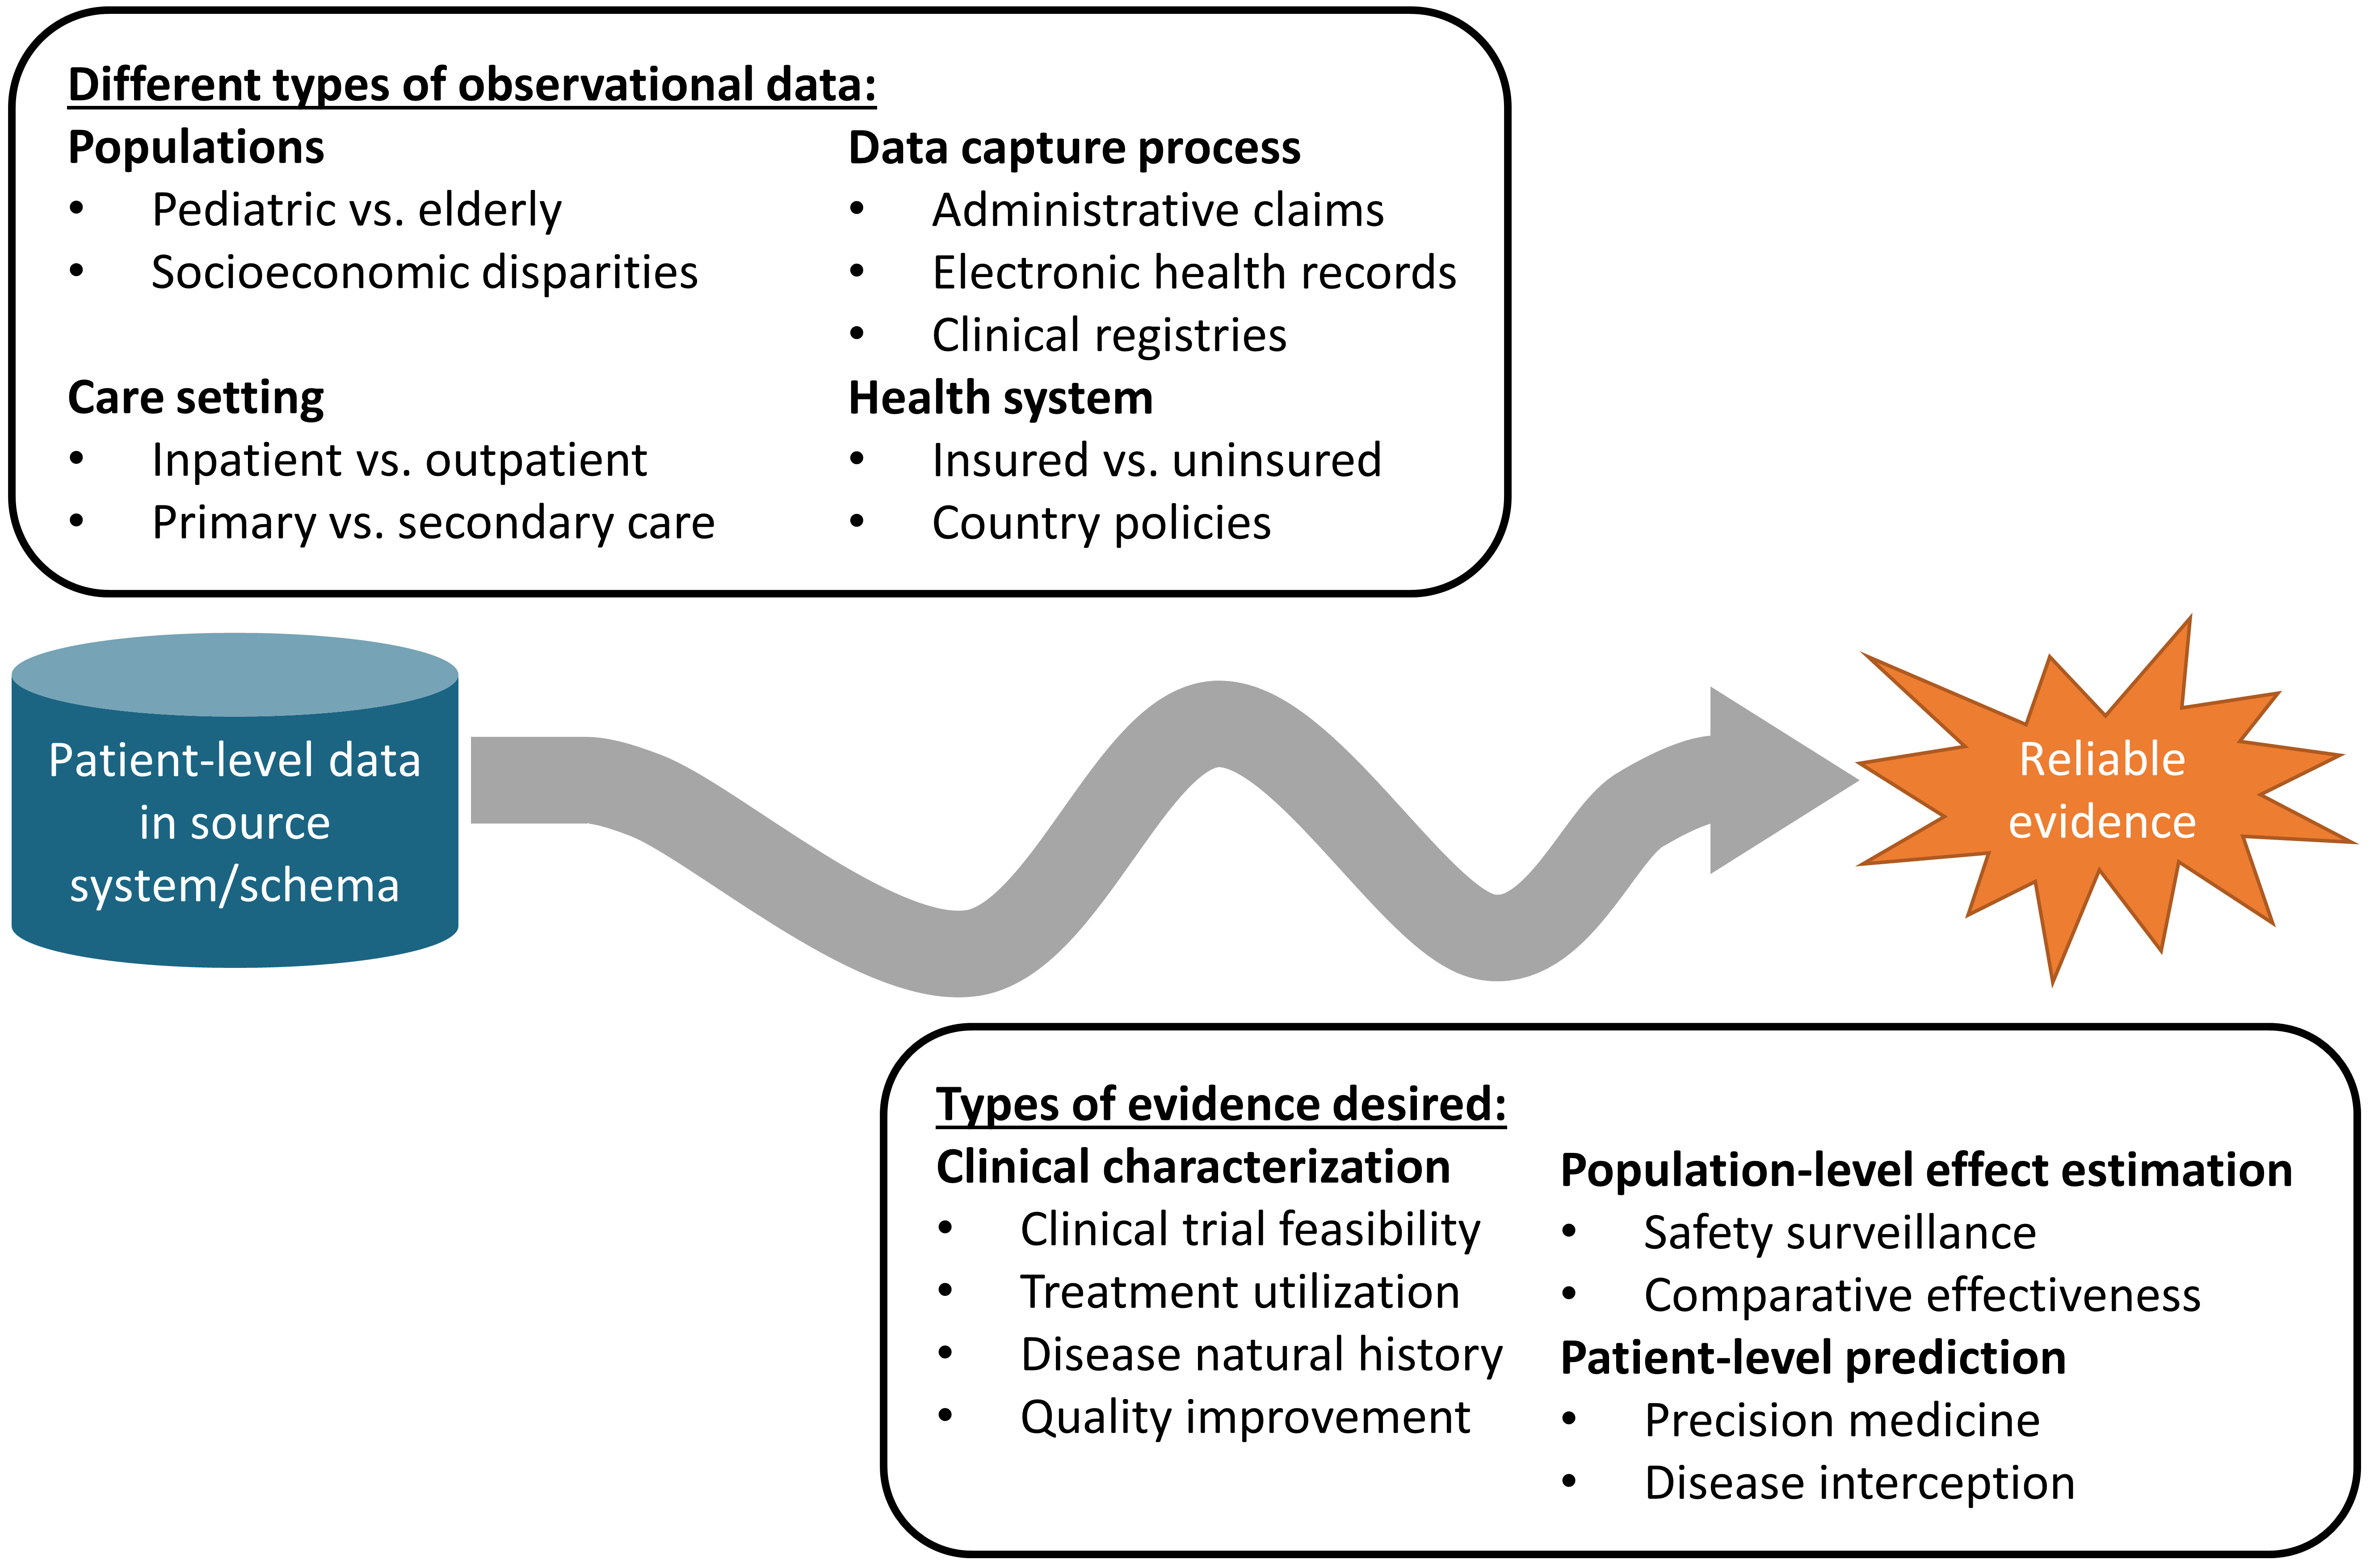
\includegraphics[width=1\linewidth]{images/OhdsiCommunity/datajourney} 

}

\caption{The journey from data to evidence}\label{fig:datajourney}
\end{figure}

원본 시스템에서 다양한 환자 수준의 데이터를 수집하는 여러 유형의 관찰
데이터베이스 (observational database)가 있다. 이 데이터베이스는 서로
다른 의료 시스템 내부의 인구, 치료 설정 및 데이터 수집 프로세스의
이질성만큼 다양하다. 의사 결정에 도움이 될 수있는 다양한 유형의 근거가
있으며, 환자 특성 분석 (clinical characterization), 인구 수준 추정
(population-level estimation) 및 환자 수준 예측 (patient-level
prediction) 으로 분류할 수 있다. 모집단 수준 영향 추정 및 환자 수준
예측의 분석 사용 사례로 분류 할 수 있습니다. 출발지 (원본 데이터) 및
원하는 목적지 (근거)와는 별도로, 여정을 수행하는 데 필요한 광범위한
임상, 과학 및 기술 역량들은 문제를 더욱 복잡하게 만든다. 보험 청구나
진료 과정이 데이터로 수집되면서 보건 정책이나 보험 환급과 관련된 행동
동기들로 인해 데이터 수집 및 정제 과정에서 발생할 수 있는 편향을
비롯하여, 환자와 의료 제공자간의 접점으로부터 원본 데이터가 발생하는
전반적인 과정에 대한 철저한 이해도 필요하다. 임상적 의문을 관련 해답을
도출하는 데 적합한 관찰 연구 설계으로 변환하기 위해선 역학 원칙과 통계적
방법을 숙지해야 한다. 수백만 명의 환자의 수년간의 종적 추적에 걸친
수십억 건의 임상 관찰을 가진 데이터셋에 대해 계산적으로 효율적인 데이터
과학 알고리즘을 구현하고 실행할 수 있는 기술적 능력 역시 필요하다.
관찰형 연구 통해 습득한 내용을 다른 종류의 근거와 통합하고, 이 새로운
지식이 건강 정책 및 임상 관행에 어떤 영향을 미칠지 결정하기 위해 임상
지식 또한 필요하다. 따라서, 한 개인이 데이터에서 근거를 성공적으로
만들어 내는 데 필요한 기술과 자원을 모두 보유하는 것은 매우 드문 일이다.
그보다는 이용 가능한 최선의 데이터를 가장 적절한 방법으로 분석하여 모든
이해당사자들이 의사결정 과정에 신뢰하고 사용할 수 있는 근거를 생산하는,
데이터에서 근거까지의 이 여정을 위해서는 보통 여러 개인과 조직의 협력이
필요하다.

\section{오몹 (Observational Medical Outcomes Partnership,
OMOP)}\label{-observational-medical-outcomes-partnership-omop}

협력 관찰형 연구 모델로써 주목할만한 예시로 오몹 (Observational Medical
Outcomes Partnership, OMOP)이 있었다. 오몹은 미국의 식품의약국 (FDA)이
주관하고, 미국 국립 보건원 (National Institutes of Health) 관리하에 학술
연구자 및 보건 데이터 파트너와 협력하는 제약 회사의 컨소시엄로
구성되었으며, 관찰형 보건의료 데이터를 이용하여 능동적 의료 제품 안전성
감시의 발전을 꾀하는 민관 협력체였다. \citep{stang2010omop} OMOP은
다수의 이해관계자 간의 거버넌스 구조를 확립했고, 다수의 청구자료 및 전자
의무 기록 데이터베이스에 적용하여 진정한 약물 안전성 연관성과 거짓 양성
소견을 식별할 수 있는 대안적인 역학 설계 및 통계 방법의 성능을
경험적으로 검증하는 일련의 방법론적 실험을 설계하였다. 분산되어 있는
관찰형 데이터 베이스를 통해 연구릴 진행함에 있어 기술적인 난제를
인식하고, 연구진들은 데이터의 구조, 내용 및 용어를 표준화하여 하나의
통계 분석 코드가 모든 데이터 파트너에서 사용될 수 있도록, OMOP 공통
데이터 모델 (Common Data Model, CDM) 을 설계하였다.
\citep{overhage2012cdm} OMOP 실험은 공통 데이터 모델과 표준화된 어휘를
확립하는 것이 가능하다는 것을 증명했다. 이는 서로 다른 관리
설정으로부터, 다른 용어 체계를 통해 다른 데이터 유형을 수용하고 하여
기관 간 협업과 효율적인 분석을 용이하게 할 수 있는 방식으로 구현되었다.

OMOP는 처음부터 연구 설계, 데이터 표준, 분석 코드, 경험적 결과 등 모든
작업 제품을 공공에 배포하여 투명성을 증진하고, OMOP가 수행하고 있는
연구에 대한 신뢰도를 쌓을 뿐 아니라, 또한 다른 이들의 연구 목적을 위하여
발전할 수 있도록 개방형 과학 (open science) 정책을 채택하였다. OMOP의
원래 초점은 약물 안전성이었지만, OMOP-CDM은 의료 처치와 보건 시스템
정책의 비교 효과성을 포함한 확대된 분석 사용 사례를 지원하기 위해
지속적으로 발전했다.

비록 OMOP이 대규모의 경험적 실험을 완성하는 데 성공하였고,
\citep{ryan2012omop, ryan2013omop} 방법론적인 혁신을 만들고,
\citep{schuemie_2014} 관찰형 데이터를 이용하여 안정성에 관련되어
의사결정에 유용한 지식 생성을 위한 적절한 방법론을 제시하였지만,
\citep{madigan_2013, madigan2013design} 이제 OMOP의 유산은 OHDSI
커뮤니티의 형성에 동기를 부여한 자극과 개방형 과학 원칙을 조기에 채택한
것으로 더 기억될 수 있다.

OMOP 프로젝트가 FDA의 능동 감시에 도움을 줄 숭 있는 관찰론적 연구를
완료하고 종료된 이후, 사람들은 OMOP 여정의 끝이, 새로운 여정의 시작이
되어야 된다고 생각했다. OMOP의 방법론적 연구가 관찰 데이터에서 생성되는
근거의 품질을 명시적으로 개선할 수 있는 과학적 모범 사례에 대한 가시적
통찰력을 제공함에도 불구하고, 그러한 모범 사례의 채택은 느렸다. 몇 가지
장애물들을 있었는데, 1) 방법론적의 혁신 이전에 관찰형 데이터 품질에 대한
근본적인 우려 2) 방법론적 문제와 해결책에 대한 불충분한 개념적 이해 3)
개별 데이터 파트너의 로컬 환경 내에서 솔루션을 독립적으로 구현할 수
없다는 점 4) 이러한 접근방식이 그들의 관심 임상 문제에 적용 가능한지에
대한 불확실성 등이었다. 이러한 모든 장애물에 대한 하나의 공통된 실마리는
한 사람만이 스스로 변화를 만드는 데 필요한 모든 것을 가지고 있지는
않지만, 여러 사람이 협력하면 이러한 문제들을 극복할 수 있다는 것이었다.

\begin{itemize}
\tightlist
\item
  기초 데이터 품질에 대한 신뢰도를 높이며 구조, 콘텐츠 및 의미론의
  일관성을 촉진하여 표준화된 분석이 가능하도록 개방형 커뮤니티의 (open
  community) 데이터 구조, 어휘 및 추출 변환 적재
  (Extract-Transform-Load, ETL)의 표준 규약 구축을 위한 협업
\item
  약물 안전성 연구 외에도 clinical characterization, population-level
  effect estimation, patient-level prediction을 위한 보다 광범위한 모범
  사례 (best practice)을 확립하기 위한 협업. 방법론적 연구를 통해 입증된
  과학적 모범 사례 구현을 코드화하고 연구자들이 쉽게 채택할 수 있는 오픈
  소스 분석 소프트웨어 개발에 대한 협업.
\item
  데이터에서 근거로의 여정을 인도해줄, 주요한 보건 문제에 대한 공동체
  공통의 질문에 대한 임상적 적용에 대한 협업
\end{itemize}

이러한 통찰을 통해, 오딧세이 (OHDSI)가 태어났다.

\section{개방형 협업 공동체로서의 오딧세이 (OHDSI as an Open-Science
Collaborative)}\label{----ohdsi-as-an-open-science-collaborative}

OHDSI (Observational Health data Sciences and Informatics, 오딧세이) 는
보다 더 나은 의료 결정과 더 나은 보건 관리를 촉진할 수 있는 과학적
근거를 공동으로 생성하도록 함으로써 보건 수준을 향상시키는 것을 목표로
하는 개방형 과학 공동체다. \citep{Hripcsak2015} OHDSI는 관찰 건강
데이터의 적절한 사용에 대한 과학적 모범 사례를 확립하기 위한 방법론적
연구를 수행하고, 이러한 연구방법론을 일관되고 투명하며 재현 가능한
솔루션으로 코드화하는 오픈 소스 분석 소프트웨어를 개발하여, 보건의료
정책 및 환자 치료에 도움이 될 수 있는 임상적 근거를 마련하는 데에 적용할
수 있도록 노력한다.

\subsection{OHDSI의 사명 (Our Mission)}\label{ohdsi--our-mission}

참여 공동체의 상호협력 하에 의료 발전을 촉진하는 근거를 생성하는 능력을
부여한다.

\begin{quote}
To improve health by empowering a community to collaboratively generate
the evidence that promotes better health decisions and better care.
\index{mission}
\end{quote}

\subsection{OHDSI의 이상 (Our Vision)}\label{ohdsi--our-vision}

의료 빅데이터의 분석을 통해 세계에 건강과 질병에 대한 포괄적인 이해를
제공한다.

\begin{quote}
A world in which observational research produces a comprehensive
understanding of health and disease. \index{vision}
\end{quote}

\subsection{OHDSI의 핵심 가치 (Our
Objectives)}\label{ohdsi---our-objectives}

\begin{itemize}
\tightlist
\item
  \textbf{혁신성 Innovation}: 우리는 적극적으로 의료 빅데이터 분석 및
  연구에 대한 혁신적인 방법론과 접근법을 찾고 격려한다.
\end{itemize}

\begin{quote}
Observational research is a field which will benefit greatly from
disruptive thinking. We actively seek and encourage fresh methodological
approaches in our work.
\end{quote}

\begin{itemize}
\tightlist
\item
  \textbf{재현성 Reproducibility}: 우리는 보건 증진을 위하여 정확하고,
  재현 가능하며, 잘 보정된 근거를 찾도록 노력한다.
\end{itemize}

\begin{quote}
Accurate, reproducible, and well-calibrated evidence is necessary for
health improvement.
\end{quote}

\begin{itemize}
\tightlist
\item
  \textbf{공동체 정신 Community}: 우리는 모든 참여자들을 환영하며
  동등하게 우리의 활동에 참여할 수 있도록 돕는다.
\end{itemize}

\begin{quote}
Everyone is welcome to actively participate in OHDSI, whether you are a
patient, a health professional, a researcher, or someone who simply
believes in our cause.
\end{quote}

\begin{itemize}
\tightlist
\item
  \textbf{개방성 Openness}: 우리는 의사 결정 과정의 투명성을 지향하며,
  우리의 진보 및 우리가 생성한 방법론, 소프트웨어, 근거를 가능한
  공개적으로 접근 가능하게 한다.
\end{itemize}

\begin{quote}
We strive to make all our community's proceeds open and publicly
accessible, including the methods, tools and the evidence that we
generate.
\end{quote}

\begin{itemize}
\tightlist
\item
  \textbf{협력 정신 Collaboration}: 우리는 참여자들의 실제적 요구를
  우선적으로 다루고, 그것을 위해 공동으로 노력한다.
\end{itemize}

\begin{quote}
We work collectively to prioritize and address the real world needs of
our community's participants.
\end{quote}

\begin{itemize}
\tightlist
\item
  \textbf{선행의 정신 Beneficence}: 우리는 고통 받는 환자를 비롯하여
  참여자 및 참여기관의 권리를 보호하기 위해 노력한다.
\end{itemize}

\begin{quote}
We seek to protect the rights of individuals and organizations within
our community at all times.
\end{quote}

\index{objectives}

\section{오딧세이의 진척 (OHDSI's Progress)}\label{--ohdsis-progress}

OHDSI는 2014년 설립된 이래 성장을 지속하여 컴퓨터 과학, 역학, 통계, 생물
의학 정보학, 보건 정책 및 임상 의학 등 다양한 분야를 대표하는 학계, 의료
제품 산업, 규제 기관, 정부, 보험자, 기술 제공자, 의료 시스템, 임상의사
및 환자 집단 2,500명 이상의 다양한 이해관계자이 온라인 포럼에서 활동하고
있다. OHDSI 협력체로써 자발적으로 보고한 기관 및 데이터베이스의 리스트는
OHDSI 웹사이트에서 확인할 수 있다. \footnote{\url{https://www.ohdsi.org/who-we-are/collaborators/}}
오딧세이 협력 지도 (Figure \ref{fig:collaboratormap}) 는 폭넓은 국제
공동체로써의 다양성을 상기시킨다.

\begin{figure}

{\centering 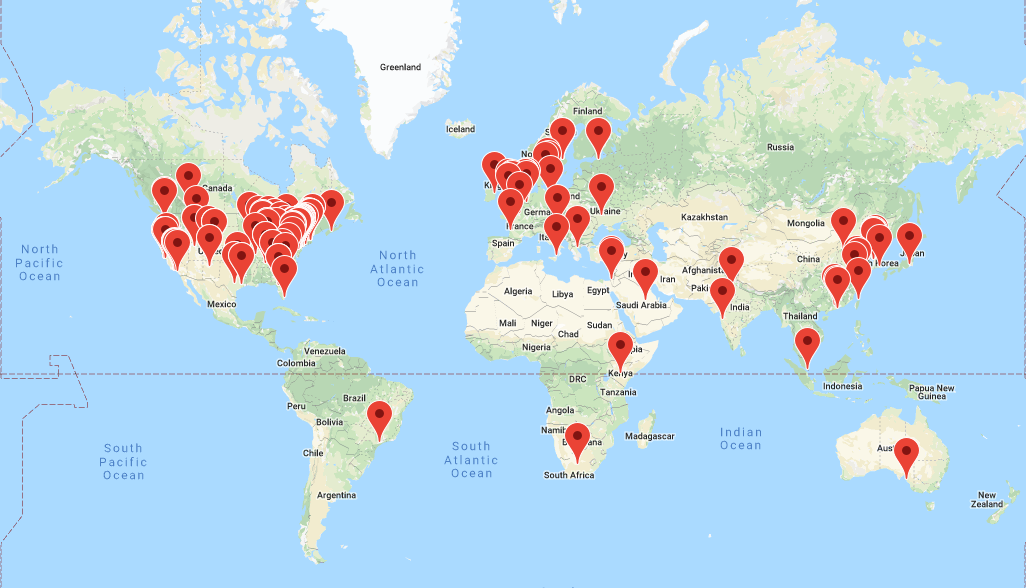
\includegraphics[width=1\linewidth]{images/OhdsiCommunity/mapOfCollaborators} 

}

\caption{Map of OHDSI collaborators as of August, 2019}\label{fig:collaboratormap}
\end{figure}

OHDSI는 OMOP-CDM이라는 개방형 공동체 데이터 표준 기반으로 2019년 8월
기준으로 20여개국, 100개 이상의 의료 데이터베이스들로 구성된 분산형
연구망 (distributed research network, DRN)을 구축했다. 분산형 연구망이란
환자 수준의 데이터를 개인이나 조직 간에 공유할 필요가 없다는 것을
의미한다. 분산연구망에서는, 데이터를 기관 폐쇄망 안에 두고 연구자는
프로토콜 형태의 분석코드/프로그램을 공유한다. 데이터 파트너들은 연구자의
요청에 따라 기관 안에서 연구 프로토콜을 실행해 자동으로 생성되는 요약
집합정보(평균, 합, 표준편차, 오즈비, 위험도 등)만 연구자에게 회신하는
방식으로, 연구자는 폐쇄망 안에 있는 환자의 개별 정보를 보거나 취득하지
않는다. OHDSI 분산망에서 각 데이터 파트너는 환자 수준 데이터의 사용에
대한 완전한 자율성을 유지하고, 각 기관의 데이터 거버넌스 정책을
지속적으로 준수한다.

OHDSI 개발자 커뮤니티는 3가지의 사용 사례를 지원하기 위해 OMOP CDM 위에
다음 3가지의 강력한 오픈 소스 분석 소프트웨어 라이브러리를 구축하였다.

\begin{enumerate}
\def\labelenumi{\arabic{enumi})}
\tightlist
\item
  Clinical characterization: 질병의 자연 경과, 치료 행태 및 질 향상을
  위한 임상 특성 분석
\item
  Population-level effect estimation: 의약품 안전성 감시 및 비교 효과
  연구에서의 인과성 분석
\item
  Patient-level prediction: 머신러닝 알고리즘을 활용한 정밀 의학 또는
  의료 개입
\end{enumerate}

OHDSI 개발자들은 또한 OMOP CDM의 채택, 데이터 품질 평가, OHDSI 네트워크
연구의 촉진을 지원하는 애플리케이션을 개발했다. 이러한 소프트웨어에는
R과 Python에 내장된 백엔드 통계 패키지 및 HTML과 Javascript로 개발된
프론트엔드 웹 어플리케이션이 포함된다. 모든 OHDSI 소프트웨어들은 오픈
소스 정책을 채택하여 Github을 통해 공개된다. \footnote{\url{https://github.com/OHDSI}}

오픈 소스 소프트웨어들과 함께, OHDSI의 개방형 과학 공동체적 접근은
관찰형 연구의 발전을 가능하게 했다. 첫번째 OHDSI 네트워크 연구는 당뇨,
우울증, 고혈압의 3가지 만성 질병에 대한 치료 패턴을 분석하는 것이었다.
PNAS(Proceedings of the National Academy of Science) 에 출판된 연구는,
그 때까지 수행된 최대 규모의 관찰형 연구로써 11개의 데이터베이스에서 2억
5천만명의 환자 데이터를 이용하여 이전에 보고된 적 없는 치료 패턴의
지역적 차이 및 환자별 치료선택에 대한 이질성에 대해 발표하였다.
\citep{Hripcsak7329} OHDSI는 교란변수를 통제하는 새로운 통계적 방법론을
제시하였고, \citep{tian_2018} 인과성 검증 능력에 대해 검증하였고,
\citep{schuemie_2018} 이러한 방법론을 뇌전증 약제의 개별 안전성 연구
\citep{duke_2017} 및 당뇨병의 이차 약제의 비교 효과 연구
\citep{vashisht_2018} 및 우울증 치료의 대규모 비교 효과 연구
\citep{schuemie_2018b}에 활용하였다. OHDSI 공동체는 또한 관찰형 보건의료
데이터의 머신러닝 알고리즘을 활용 프레임 워크를 구축 \citep{reps2018}
하여 다양한 치료 분야에 활용하였다.
\citep{johnston_2019, cepeda_2018, reps_2019}

\section{Collaborating in OHDSI}\label{collaborating-in-ohdsi}

OHDSI는 근거를 생성하기 위해 협업을 강화하는 것을 목표로 하는
공동체인데, OHDSI 참가자가 된다는 것은 무엇을 의미하는가? 만약 당신이
OHDSI의 사명을 믿고 데이터에서 근거에 이르는 여정의 어디든지 기여를 하는
데 관심이 있다면, OHDSI는 당신을 위한 공동체가 될 수 있다. OHDSI
참가자는 보건 의료 데이터에 접근이 가능하고, 이를 활용해 의학적 근거를
생성하고 싶은 개인일 수 있다. OHDSI 참가자는 과학적 모범 사례를 수립하고
대안적 접근법을 평가하는 데 관심이 있는 방법론 연구자일 수 있다. OHDSI
참가자는 OHDSI의 타 연구자들이 사용할 수 있는 도구를 만들기 위해
프로그래밍 기술을 적용하는 데 관심이 있는 소프트웨어 개발자일 수 있다.
OHDSI 참가자는 중요한 의학보건학적 질문을 가지고 있고 논문 발표 등을
통해 그러한 질문들에 대한 근거를 보다 더 큰 의료 커뮤니티에 제공하고자
하는 임상 연구자일 수 있다. OHDSI 참가자는 공공 보건을 위해 이러한
공통적인 사명과 가치를 믿고 해당 지역의 공동체가 OHDSI 관련 교육과
심포지엄 개최를 포함하여, 그 임무를 지속할 수 있도록 자원을 제공하는
개인 또는 단체일 수도 있다. 당신의 배경이나 소속과 관계없이, OHDSI는
개개인이 공통의 목적을 위해 함께 일할 수 있는 공동체가 되기를 추구하고
있으며, 각 개인이 공동으로 의료 서비스를 발전시킬 수 있는 기여를 하고
있다. 이 여정에 함께하고 싶다면, 챕터 \ref{WhereToBegin} (``Where To
Begin'') 를 통해 어떻게 시작하는 지 배울 수 있다.

\section{한국 오딧세이의 역사}\label{--}

아주대학교 박래웅 교수가 아주대 병원의 전자의무기록을 이용하여 2014년
OMOP-CDM 도입을 시작하였고, 2015년 첫 연례 심포지엄에서 활용 결과를
발표하면서 한국의 OHDSI 참여가 시작되었다. 이후 계속적으로 한국에서
OMOP-CDM, OHDSI 전파를 위해 노력하였고, 2016년부터는 최초로 국제 OHDSI
committee에서 개별 국가를 위한 포럼
\href{http://forums.ohdsi.org/c/For-collaborators-wishing-to-communicate-in-Korean}{Korean
chapter}을 개설하고, 한국의 OHDSI 참여를 독려하였다. 첫 한국 국제
오딧세이 심포지엄은 2017년 3월 아주대학교에서 튜토리얼, 리더십 미팅을
포함하여 3일간 개최되었다.

\begin{figure}
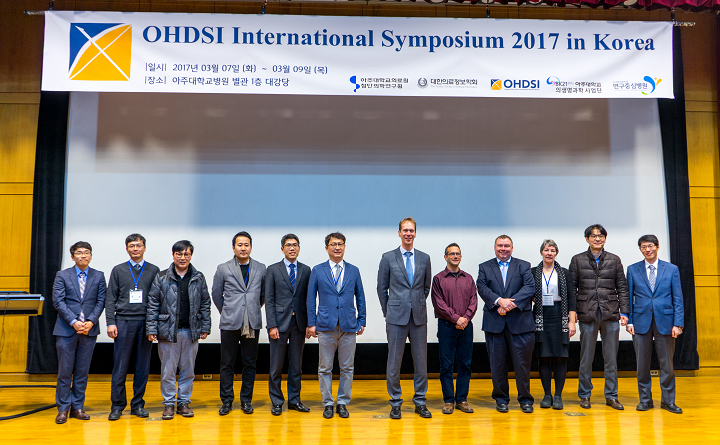
\includegraphics[width=0.8\linewidth]{images/OhdsiCommunity/DSC01956} \caption{OHDSI International Symposium 2017 in Korea}\label{fig:OHDSIInternationalSymposium2017inKorea1}
\end{figure}\begin{figure}
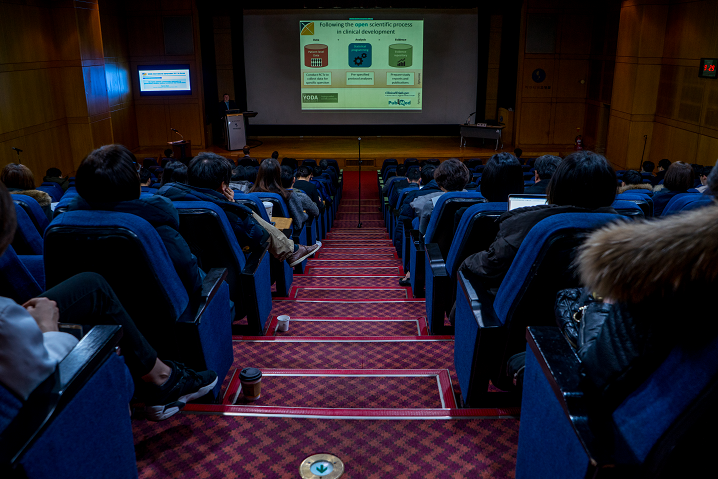
\includegraphics[width=0.8\linewidth]{images/OhdsiCommunity/DSC01861} \caption{OHDSI International Symposium 2017 in Korea}\label{fig:OHDSIInternationalSymposium2017inKorea1}
\end{figure}

\begin{figure}
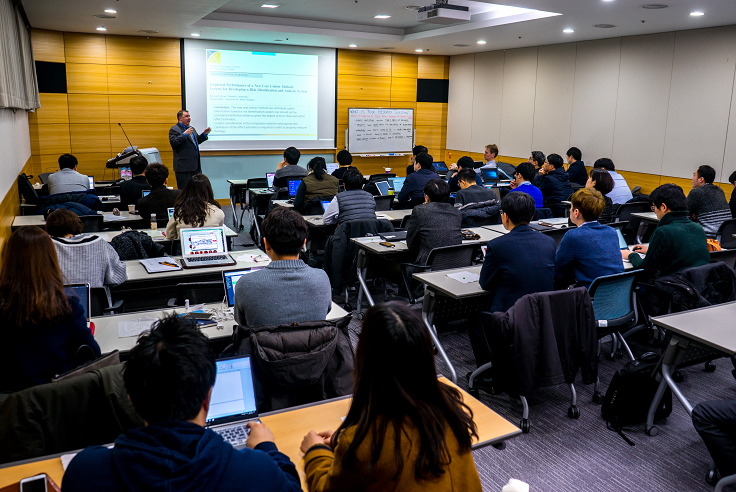
\includegraphics[width=0.8\linewidth]{images/OhdsiCommunity/DSC02166} \caption{Tutorial in the OHDSI International Symposium 2017}\label{fig:OHDSIInternationalSymposium2017inKorea2}
\end{figure}

한국 OHDSI 네트워크에 참여를 희망하는 병원 관계자들과 함께 2017년 3월
7일 첫번째 리더십 미팅을 가진 후 현재까지 2달마다 전국의 의과대학/병원을
순회하며 한국 OHDSI 리더십 미팅을 개최하며 OHDSI 전파 및 상호 협력을
꾀하고 있다.

\section{Summary}\label{summary}

\BeginKnitrBlock{rmdsummary}
\begin{itemize}
\item
  OHDSI의 사명은 참여 공동체의 상호협력 하에 의료 발전을 촉진하는 근거를
  생성하는 능력을 부여하는 것이다.
\item
  OHDSI의 이상은 혁신성, 재현성, 공동체 정신, 개방성, 협력 정신, 선행의
  정신을 바탕으로 의료 빅데이터의 분석을 통해 세계에 건강과 질병에 대한
  포괄적인 이해를 제공하는 것이다.
\item
  OHDSI 참가자들은 개방형 공동체로서의 데이터 표준, 방법론 연구,
  오픈소스 분석 소프트웨어 개발 및 임상적 적용을 통해 데이터로부터
  근거로의 여정을 발전시키고자 노력한다.
\end{itemize}
\EndKnitrBlock{rmdsummary}

\chapter{Where to Begin}\label{WhereToBegin}

\emph{Chapter leads: Hamed Abedtash \& Kristin Kostka}

\begin{quote}
``A journey of a thousand miles begins with a single step.'' - Lao Tzu
\end{quote}

The OHDSI community represents a mosaic of stakeholders across academia,
industry and government-entities. Our work benefits a range of
individuals and organizations, including patients, providers, and
researchers, as well as health care systems, industry, and government
agencies. This benefit is achieved by improving both the quality of
healthcare data analytics as well as the usefulness of healthcare data
to these stakeholders. We believe observational research is a field
which benefits greatly from disruptive thinking. We actively seek and
encourage fresh methodological approaches in our work. \index{community}

\section{Join the Journey}\label{join-the-journey}

Everyone is welcome to actively participate in OHDSI, whether you are a
patient, a health professional, a researcher, or someone who simply
believes in our cause. OHDSI maintains an inclusive membership model. To
become an OHDSI collaborator requires no membership fee. Collaboration
is as simple as raising a hand to be included in the yearly OHDSI
membership count. Involvement is entirely at-will. A collaborator can
have any level of contribution within the community, ranging from
someone who attends weekly community calls to leading network studies or
OHDSI working groups. Collaborators do not have to be data holders to be
considered active members of the community. The OHDSI community aims to
serve data holders, researchers, health care providers and patients \&
consumers alike. A record of collaborator profiles are maintained and
periodically updated on the OHDSI website. Membership is fostered via
OHDSI community calls, workgroups and regional
chapters.\index{join the journey} \index{workgroups} \index{chapters}

\begin{figure}

{\centering 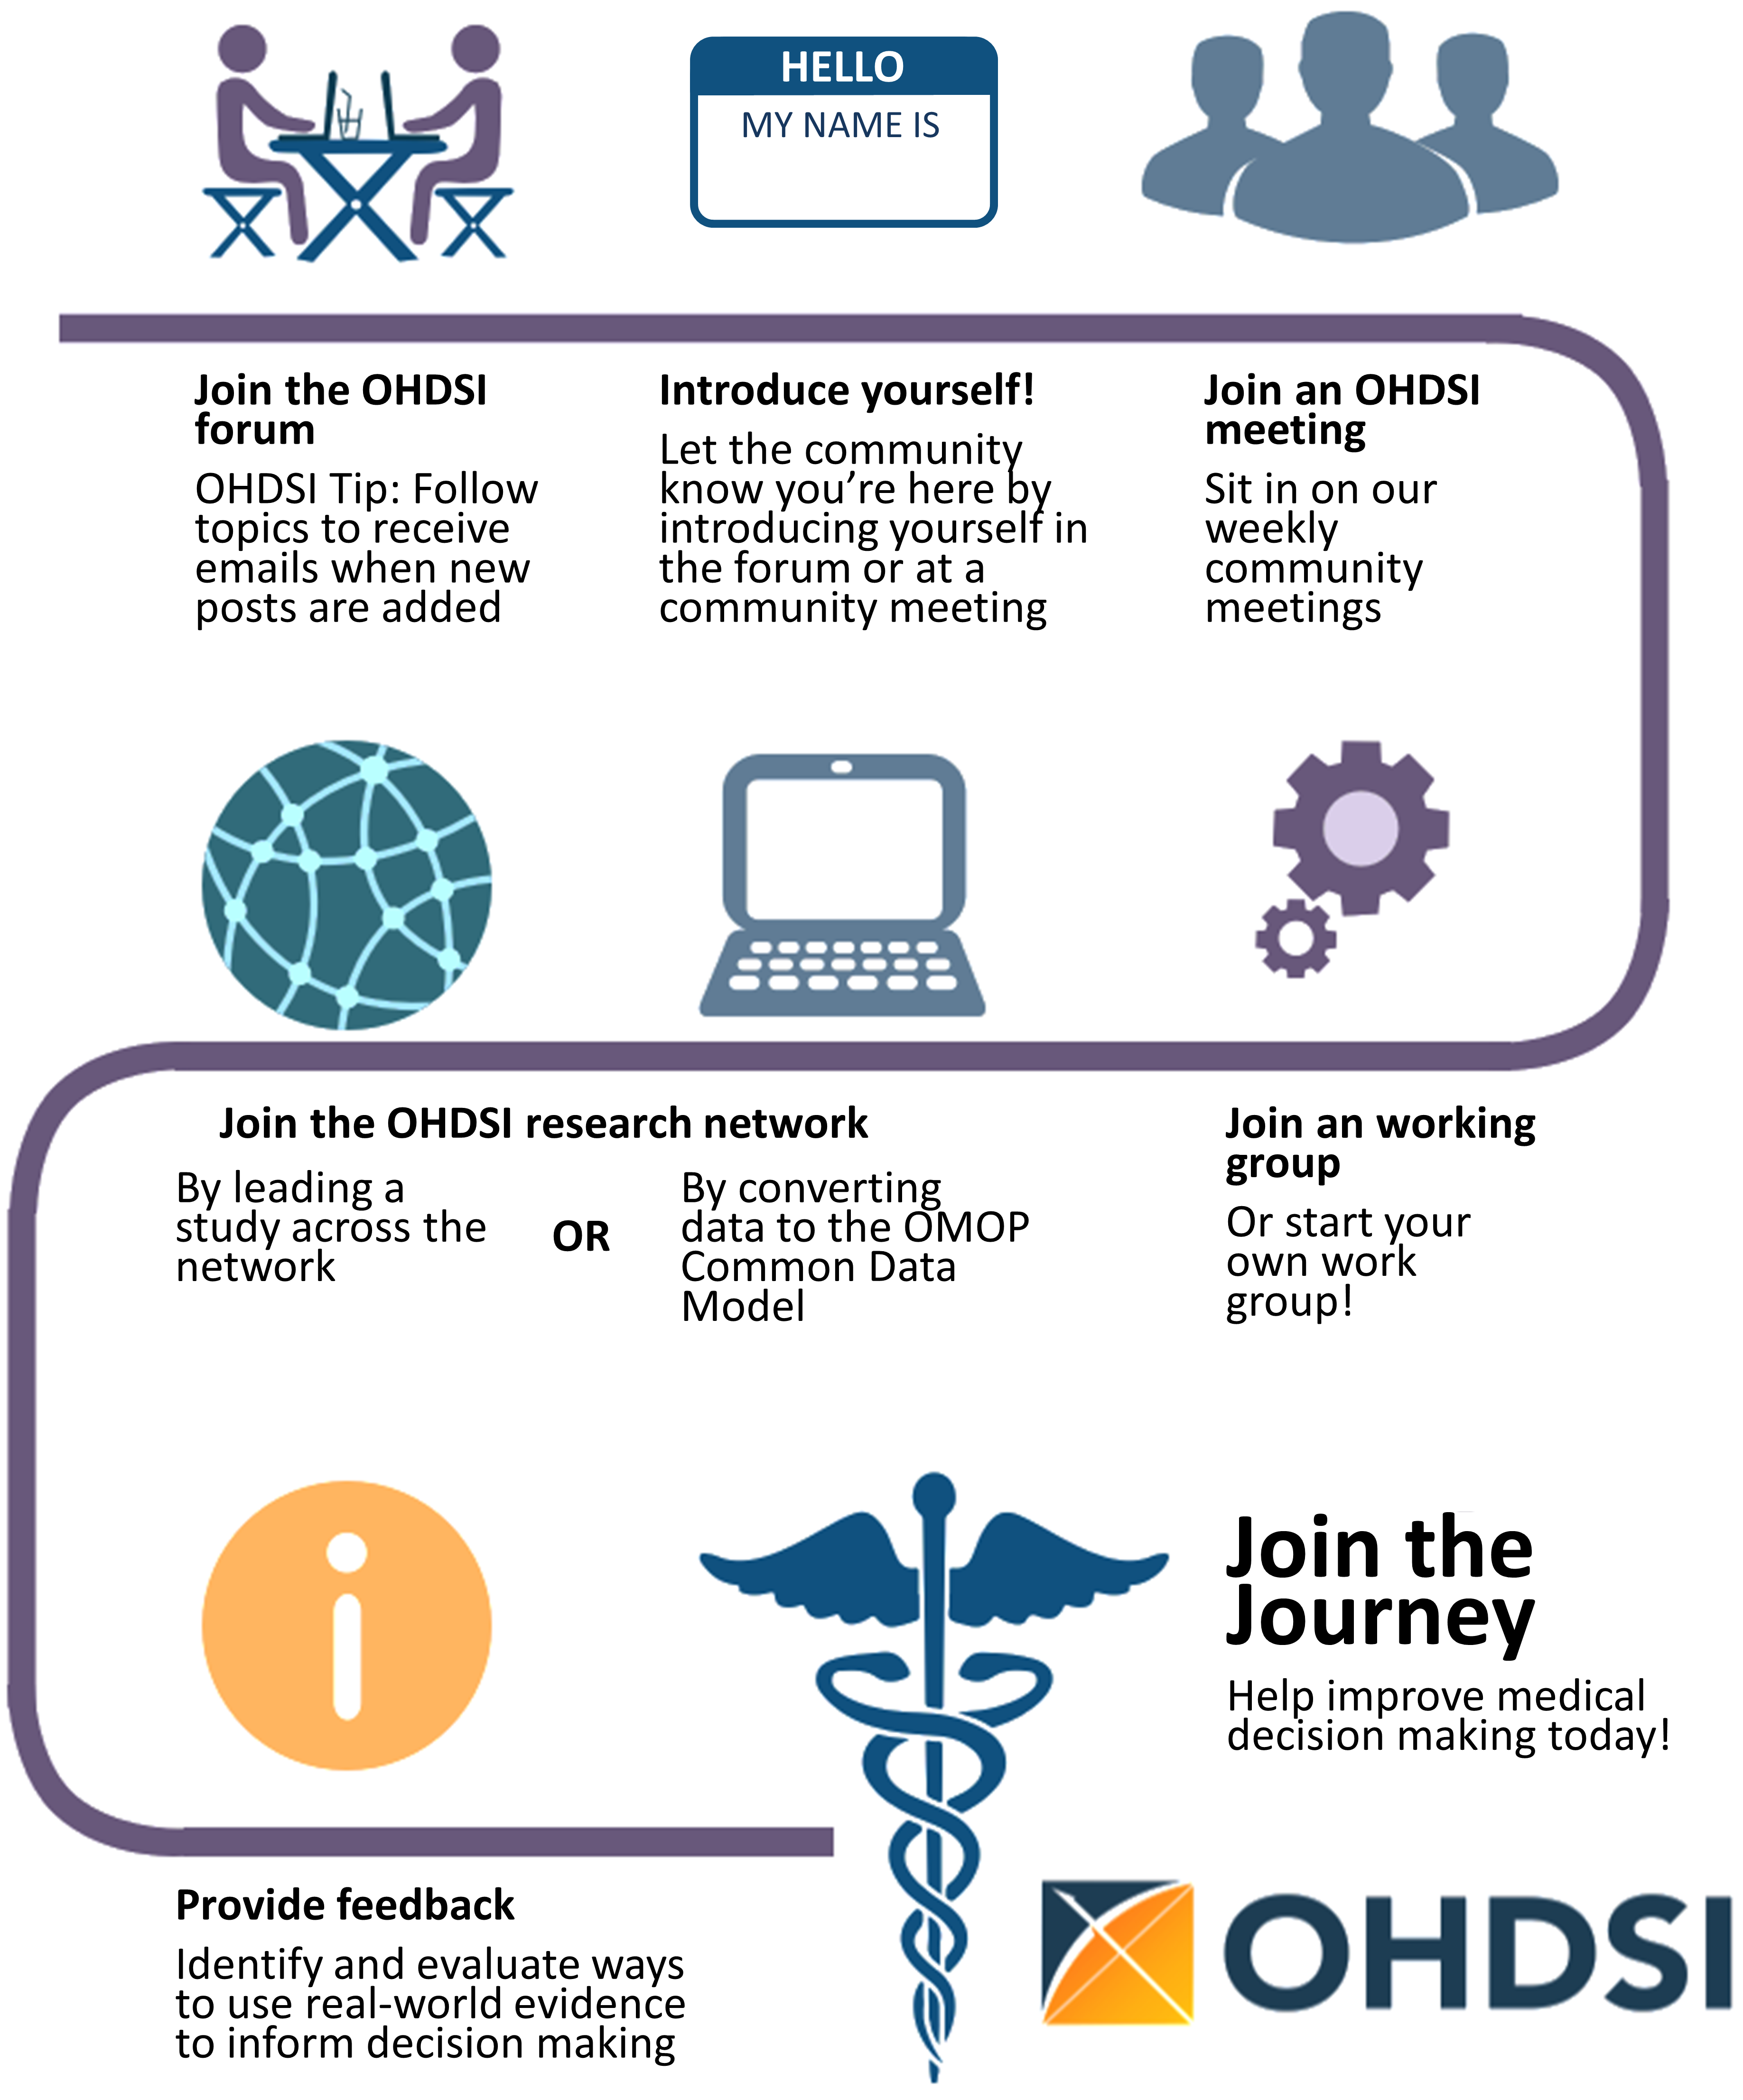
\includegraphics[width=0.9\linewidth]{images/WhereToBegin/joinTheJourney} 

}

\caption{Join the journey - How to become an OHDSI collaborator.}\label{fig:jointhejourney}
\end{figure}

\subsection{OHDSI Forums}\label{ohdsi-forums}

The OHDSI Forums\footnote{\url{http://forum.ohdsi.org}} is an online
discussion site where OHDSI Community Collaborators can hold
conversations in the form of posted messages. The forums consist of a
tree-like directory structure. The top end is ``Categories''. The forums
can be divided into categories for the relevant discussions. Under the
categories are sub-forums and these sub-forums can further have more
sub-forums. The topics (commonly called threads) come under the lowest
level of sub-forums and these are the places under which forums members
can start their discussions or posts.

In the OHDSI forums, you can find categories of content including:

\begin{itemize}
\tightlist
\item
  \textbf{General:} for general discussion about the OHDSI community and
  how to get involved
\item
  \textbf{Implementers:} for discussion about how to implement the
  Common Data Model and OHDSI analytics framework in your local
  environment
\item
  \textbf{Developers:} for discussion around open-sourced development of
  OHDSI applications and other tools that leverage the OMOP CDM
\item
  \textbf{Researchers:} for discussion around CDM-based research,
  including evidence generation, collaborative research, statistical
  methods and other topics of interest to the OHDSI Research Network
\item
  \textbf{CDM Builders:} for discussion of ongoing CDM development,
  including requirements, vocabulary, and technical aspects
\item
  \textbf{Vocabulary Users:} for discussion around vocabulary content
\item
  \textbf{Regional Chapters (e.g.~Korea, China, Europe):} for regional
  discussions in their native languages related to local OMOP
  implementations and OHDSI community activities
\end{itemize}

To begin posting your own topics, you will need to sign up for an
account. Once you have a forums account, you are encouraged to introduce
yourself on the General Topic under the thread called ``Welcome to
OHDSI! - Please introduce yourself''. You are invited to reply and 1)
Introduce yourself and tell us a bit about what you do and 2) Let us
know how you'd like to help out in the community (ex. software
development, run studies, write research papers, etc). Now you are on
your OHDSI Journey! From here, you are encouraged to join in the
discussion. The OHDSI Community encourages using the Forums as your way
to ask questions, discuss new ideas and collaborate. \index{forum}

\BeginKnitrBlock{rmdimportant}
You can select topics to ``watch.'' What this means is whenever a new
post is added in a topic you're watching, you will receive an email and
be able to reply to the post directly through your email. Watch the
general thread to recieve details about upcoming meeting agendas,
collaboration opportunities and have the weekly OHDSI digest delivered
directly to your inbox!
\EndKnitrBlock{rmdimportant}

\subsection{OHDSI Events}\label{ohdsi-events}

OHDSI regularly holds in-person events to provide opportunities for
collaborators to learn from each other and connect to foster future
collaborations. These events are communicated on the OHDSI website, and
are free for anyone interested in attending.

OHDSI Symposia are scientific conferences, held annually in US, Europe,
and Asia, where collaborators can present their latest research through
plenary talks, poster presentations, and software demonstrations. OHDSI
Symposia provide a great venue for networking and to learn about the
most recent progress across the community. OHDSI Symposia are generally
accompanied by OHDSI tutorials, taught by fellow OHDSI collaborators as
the course faculty, which provide community newcomers the opportunity
for hands-on engagement on topics around data standards and analysis
best practices. These tutorials are generally video-recorded and made
available on the OHDSI website after the events for those who can't make
it in person.

OHDSI Collaborator face-to-face events are smaller fora which are
typically centered on a problem of shared interest to focus on during
the time together. Past events have included a phenotype hack-a-thon,
and data quality hack-a-thon, and open-source software
documentation-a-thon. OHDSI has hosted multiple Study-a-thon events,
where the goal of the multi-day session is to collaborate as a team on a
particular research question by designing and implementing an
appropriate observational analysis, executing the study across the OHDSI
network, and synthesizing the evidence for public dissemination. In all
of these events, there is a shared desire to solve a common problem but
also a shared interest in providing a welcoming environment that
encourages learning and continuous improvement on the process of
collaborative problem-solving.

Learn more about the power of the OHDSI Community. Explore past
symposiums, face-to-face meetings and watch OHDSI tutorials by visiting
the \href{https://www.ohdsi.org/past-events/}{OHDSI Past Events section}
on the OHDSI website. Past Events is updated regularly to archive
community events.

\subsection{OHDSI Community Calls}\label{ohdsi-community-calls}

OHDSI Community Calls are a weekly opportunity to spotlight ongoing
activity within the OHDSI community. Held every Tuesday from 12-1pm ET,
these teleconferences are a time for the OHDSI community to come
together to share recent developments and recognize the accomplishments
of individual collaborators, working groups and the community as a
whole. Each week's meeting is recorded, and presentations are archived
in the OHDSI website resources.

All OHDSI Collaborators are welcome to participate in this weekly
teleconference and encouraged to propose topics for community
discussion. OHDSI Community Calls can be a forum to share research
findings, present and seek feedback for active works-in-progress,
demonstrate open-source software tools under development, debate
community best practices for data modeling and analytics, and brainstorm
future collaborative opportunities for grants/publications/conference
workshops. If you are a Collaborator with a topic for an upcoming OHDSI
Collaborator meeting, you are invited to post your thoughts on the OHDSI
Forums.

As a newcomer to the OHDSI community, it is encouraged to add this call
series to your calendar to get acquainted with what is happening across
the OHDSI network. If you would like to join an OHDSI call, please
consult the
\href{https://www.ohdsi.org/web/wiki/doku.php?id=projects:ohdsi_community}{OHDSI
wiki}. Community call topics vary from week-to-week. You can also
consult the OHDSI Weekly Digest on the OHDSI forum for more information
on weekly presentation topics. Newcomers are invited to introduce
themselves on their first call and tell the community about themselves,
their background and what brought them to OHDSI.
\index{community!community calls}

\subsection{OHDSI Workgroups}\label{ohdsi-workgroups}

OHDSI has a variety of ongoing projects lead by workgroup teams. Each
workgroup has its own leadership team which determine the project's
objectives, goals and artifacts to be contributed to the community.
Workgroup participation is open to all who have an interest in
contributing to the project objectives and goals. Workgroups may be
long-standing, strategic objectives or short-term projects to accomplish
a specific need in the community. Workgroup meeting cadence is
determined by the project leadership and will vary from group to group.
A list of the active workgroups is maintained on the
\href{https://www.ohdsi.org/web/wiki/doku.php?id=projects:overview}{OHDSI
Wiki}. \index{workgroups}

Table \ref{tab:OHDSIworkgroups} provides a quick reference to active
OHDSI workgroups. You are encouraged to join a call and learn more.

\begin{longtable}[]{@{}lll@{}}
\caption{\label{tab:OHDSIworkgroups} Notable OHDSI
Workgroups}\tabularnewline
\toprule
\begin{minipage}[b]{0.08\columnwidth}\raggedright\strut
Workgroup Name\strut
\end{minipage} & \begin{minipage}[b]{0.25\columnwidth}\raggedright\strut
Objective\strut
\end{minipage} & \begin{minipage}[b]{0.14\columnwidth}\raggedright\strut
Target Audience\strut
\end{minipage}\tabularnewline
\midrule
\endfirsthead
\toprule
\begin{minipage}[b]{0.08\columnwidth}\raggedright\strut
Workgroup Name\strut
\end{minipage} & \begin{minipage}[b]{0.25\columnwidth}\raggedright\strut
Objective\strut
\end{minipage} & \begin{minipage}[b]{0.14\columnwidth}\raggedright\strut
Target Audience\strut
\end{minipage}\tabularnewline
\midrule
\endhead
\begin{minipage}[t]{0.08\columnwidth}\raggedright\strut
Atlas \& WebAPI\strut
\end{minipage} & \begin{minipage}[t]{0.25\columnwidth}\raggedright\strut
Atlas and WebAPI are part of the OHDSI open-source software architecture
that aim to provide standardized analytic capabilities built on the
foundation of the OMOP Common Data Model.\strut
\end{minipage} & \begin{minipage}[t]{0.14\columnwidth}\raggedright\strut
Java \& JavaScript software developers aiming to improve and contribute
to the open-source Atlas/WebAPI platform\strut
\end{minipage}\tabularnewline
\begin{minipage}[t]{0.08\columnwidth}\raggedright\strut
CDM \& Vocabulary\strut
\end{minipage} & \begin{minipage}[t]{0.25\columnwidth}\raggedright\strut
To continue to develop the OMOP Common Data Model for the purpose of
systematic, standardized and large-scale analytics applied to clinical
patient data. To improve the quality of the Standardized Vocabularies by
increasing their coverage of international coding systems and clinical
aspects of patient care in order to support the standardized analytics
developed by other working groups.\strut
\end{minipage} & \begin{minipage}[t]{0.14\columnwidth}\raggedright\strut
Any who has an interest in improving the OMOP Common Data Model and
Standardized Vocabularies to meet all needs and use cases\strut
\end{minipage}\tabularnewline
\begin{minipage}[t]{0.08\columnwidth}\raggedright\strut
Genomics\strut
\end{minipage} & \begin{minipage}[t]{0.25\columnwidth}\raggedright\strut
Expand the OMOP CDM to incorporate genomic data from patients. The group
will define a CDM-compatible schema that can store information for
genetic variants from various sequencing process.\strut
\end{minipage} & \begin{minipage}[t]{0.14\columnwidth}\raggedright\strut
Open to all\strut
\end{minipage}\tabularnewline
\begin{minipage}[t]{0.08\columnwidth}\raggedright\strut
Population-Level Estimation\strut
\end{minipage} & \begin{minipage}[t]{0.25\columnwidth}\raggedright\strut
Develop scientific methods for observational research leading to
population level estimates of effects that are accurate, reliable, and
reproducible, and facilitate the use of these methods by the
community.\strut
\end{minipage} & \begin{minipage}[t]{0.14\columnwidth}\raggedright\strut
Open to all\strut
\end{minipage}\tabularnewline
\begin{minipage}[t]{0.08\columnwidth}\raggedright\strut
Natural Language Processing\strut
\end{minipage} & \begin{minipage}[t]{0.25\columnwidth}\raggedright\strut
To promote the use of textual information from Electronic Health Records
(EHRs) for observational studies under the OHDSI umbrella. To facilitate
this objective, the group will develop methods and software that can be
implemented to utilize clinical text for studies by the OHDSI
community.\strut
\end{minipage} & \begin{minipage}[t]{0.14\columnwidth}\raggedright\strut
Open to all\strut
\end{minipage}\tabularnewline
\begin{minipage}[t]{0.08\columnwidth}\raggedright\strut
Patient-Level Prediction\strut
\end{minipage} & \begin{minipage}[t]{0.25\columnwidth}\raggedright\strut
establish a standardized process for developing accurate and
well-calibrated patient-centered predictive models that can be utilized
for multiple outcomes of interest and can be applied to observational
healthcare data from any patient subpopulation of interest\strut
\end{minipage} & \begin{minipage}[t]{0.14\columnwidth}\raggedright\strut
Open to all\strut
\end{minipage}\tabularnewline
\begin{minipage}[t]{0.08\columnwidth}\raggedright\strut
Gold Standard Phenotype Library\strut
\end{minipage} & \begin{minipage}[t]{0.25\columnwidth}\raggedright\strut
To enable members of the OHDSI community to find, evaluate, and utilize
community-validated cohort definitions for research and other
activities\strut
\end{minipage} & \begin{minipage}[t]{0.14\columnwidth}\raggedright\strut
Open to all with an interest in curation and validation of
phenotypes\strut
\end{minipage}\tabularnewline
\begin{minipage}[t]{0.08\columnwidth}\raggedright\strut
FHIR Workgroup\strut
\end{minipage} & \begin{minipage}[t]{0.25\columnwidth}\raggedright\strut
To establish the roadmap for the OHDSI FHIR integration and to make
recommendations to the broader community for leveraging the FHIR
implementation and data in EHR community for the OHDSI-based observation
studies and for disseminating the OHDSI data and research results
through the FHIR-based tools and APIs.\strut
\end{minipage} & \begin{minipage}[t]{0.14\columnwidth}\raggedright\strut
Open to all with an interest in interoperability\strut
\end{minipage}\tabularnewline
\begin{minipage}[t]{0.08\columnwidth}\raggedright\strut
GIS\strut
\end{minipage} & \begin{minipage}[t]{0.25\columnwidth}\raggedright\strut
Expand the OMOP CDM and leverage OHDSI tools so that patients'
environmental exposure histories can be related to their clinical
phenotypes\strut
\end{minipage} & \begin{minipage}[t]{0.14\columnwidth}\raggedright\strut
Open to all with an interest in health-related geographic
attributes\strut
\end{minipage}\tabularnewline
\begin{minipage}[t]{0.08\columnwidth}\raggedright\strut
Clinical Trials\strut
\end{minipage} & \begin{minipage}[t]{0.25\columnwidth}\raggedright\strut
Understand clinical trial use cases where the OHDSI platform \&
ecosystem can aid trials in any aspect, and assist in driving updates in
OHDSI tools to support.\strut
\end{minipage} & \begin{minipage}[t]{0.14\columnwidth}\raggedright\strut
Open to all with an interest in clinical trials\strut
\end{minipage}\tabularnewline
\begin{minipage}[t]{0.08\columnwidth}\raggedright\strut
THEMIS\strut
\end{minipage} & \begin{minipage}[t]{0.25\columnwidth}\raggedright\strut
The objective of THEMIS is to develop standard conventions, above and
beyond the OMOP CDM conventions, to ensure ETL protocols designed at
each OMOP site are of highest quality, reproducible and efficient.\strut
\end{minipage} & \begin{minipage}[t]{0.14\columnwidth}\raggedright\strut
\strut
\end{minipage}\tabularnewline
\begin{minipage}[t]{0.08\columnwidth}\raggedright\strut
Metadata \& Annotations\strut
\end{minipage} & \begin{minipage}[t]{0.25\columnwidth}\raggedright\strut
Our goal is to define a standard process for storing human- and
machine-authored metadata and annotations in the Common Data Model to
ensure researchers can consume and create useful data artifacts about
observational data sets.\strut
\end{minipage} & \begin{minipage}[t]{0.14\columnwidth}\raggedright\strut
Open to all\strut
\end{minipage}\tabularnewline
\begin{minipage}[t]{0.08\columnwidth}\raggedright\strut
Patient Generated Health Data (PGHD)\strut
\end{minipage} & \begin{minipage}[t]{0.25\columnwidth}\raggedright\strut
The goal of this WG would be developing ETL conventions, integration
process with clinical data, and analytic process for PGHD, which is
generated through Smart Phone/App/Wearable devices.\strut
\end{minipage} & \begin{minipage}[t]{0.14\columnwidth}\raggedright\strut
Open to all\strut
\end{minipage}\tabularnewline
\begin{minipage}[t]{0.08\columnwidth}\raggedright\strut
Women of OHDSI\strut
\end{minipage} & \begin{minipage}[t]{0.25\columnwidth}\raggedright\strut
To provide a forum for women within the OHDSI community to come together
and discuss challenges they face as women working in science,
technology, engineering and mathematics (STEM). We aim to facilitate
discusses where women can share their perspectives, raise concerns,
propose ideas on how the OHDSI community can support women in STEM, and
ultimately inspire women to become leaders within the community and
their respective fields.\strut
\end{minipage} & \begin{minipage}[t]{0.14\columnwidth}\raggedright\strut
Open to all who identify with this mission\strut
\end{minipage}\tabularnewline
\begin{minipage}[t]{0.08\columnwidth}\raggedright\strut
Steering Committee\strut
\end{minipage} & \begin{minipage}[t]{0.25\columnwidth}\raggedright\strut
To uphold OHDSI's mission vision and values by ensuring all OHDSI
activities and events are aligned with the needs of our growing
community. In addition, the group serves as an advisory group for the
OHDSI coordinating center based at Columbia by providing guidance for
OHDSI's future direction.\strut
\end{minipage} & \begin{minipage}[t]{0.14\columnwidth}\raggedright\strut
Leaders within the community\strut
\end{minipage}\tabularnewline
\bottomrule
\end{longtable}

\subsection{OHDSI Regional Chapters}\label{ohdsi-regional-chapters}

An OHDSI regional chapter represents a group of OHDSI collaborators
located in a geographic area who wish to hold local networking events
and meetings to address problems specific to their geographic location.
Today, OHDSI regional chapters include OHDSI in Europe\footnote{\url{https://www.ohdsi-europe.org/}},
OHDSI in South Korea\footnote{\url{http://forums.ohdsi.org/c/For-collaborators-wishing-to-communicate-in-Korean}}
and OHDSI in China.\footnote{\url{https://ohdsichina.org/}} If you would
like to set-up an OHDSI regional chapter in your region, you may do so
by following the OHDSI regional chapter process outlined on the
\href{https://www.ohdsi.org/who-we-are/regional-chapters}{OHDSI
website}. \index{chapters}

\subsection{OHDSI Research Network}\label{ohdsi-research-network}

Many OHDSI collaborators are interested in converting their data into
the OMOP Common Data Model. The OHDSI research network represents a
diverse, global community of observational databases that have undergone
Extract-Transform-Load (ETL) processes to become OMOP compliant. If your
journey in the OHDSI community includes transforming data, there are
numerous community resources available to aid you in your journey
including tutorials on the OMOP CDM and Vocabularies, freely available
tools to assist with conversion, and workgroups targeting specific
domains or types of data conversions. The OHDSI collaborators are
encouraged to utilize the OHDSI forum to discuss and troubleshoot
challenges that arise during CDM conversions.

\section{Where You Fit In}\label{where-you-fit-in}

By now, you may be wondering: \emph{where do I fit into the OHDSI
Community?}

\textbf{I am a clinical researcher looking to start a study.} If you are
a clinical researcher interesting in using the OHDSI Research Network to
answer a specific question -- maybe even publish a paper -- you're in
the right place. You can start by posting your idea to the
\href{https://forums.ohdsi.org/c/researchers}{OHDSI Researchers Topic}
on the OHDSI Forum. This will help you connect with researchers of
similar interest. OHDSI loves to publish and has many resources
available to expedite turning your research question into an analysis
and a paper. You can find more information in Chapters
\ref{Characterization}, \ref{PopulationLevelEstimation}, and
\ref{PatientLevelPrediction}.

\textbf{I want to read and consume the information the OHDSI community
is produce.} Whether you're a patient, a practicing clinician or subject
matter expertise in healthcare, OHDSI wants to provide you with high
quality evidence to help you better understand health outcomes. Maybe
it's been a while since you have written code. Maybe you never program.
You have a place in this community. We call you an \emph{evidence
consumer} -- you are the individuals who are turning OHDSI research into
action. You are sifting through to know what evidence OHDSI has
generated and is generating, possibly also wanting to suggest questions
relevant for you. We welcome you to join the discussion. Start asking
questions on the \href{http://forum.ohdsi.org}{OHDSI Forum}. Attend
Community Calls and hear about the latest research. Attend the OHDSI
Symposiums and Face-to-Face Meetings to engage directly with the
community. Your questions are an important part of the OHDSI community.
Speak up and help us learn more about what evidence you are searching
for!

\textbf{I work in a healthcare leadership role. I may be a data owner
and/or represent one. I am evaluating the utility of the OMOP CDM and
OHDSI analytical tools for my organization.} As an administrator/leader
of an organization, you may have heard about OHDSI and are curious to
know the OMOP CDM could work for your use cases. You may start by
looking through \href{https://www.ohdsi.org/past-events/}{OHDSI Past
Events} materials to see the body of research. You may join a Community
Call and simply listen in. You may also find that Chapter
\ref{DataAnalyticsUseCases} (Data Analytics Use Cases) helps you
understand the kind of research the OMOP CDM and OHDSI analytics tools
can enable. The OHDSI Community is here for you in your journey. Don't
be afraid to speak up and ask for examples if you have specific areas
you're interested in. More than 200 organizations around the world are
collaborating in OHDSI, there's plenty of success stories to help
showcase the value of this community.

\textbf{I am a database administrator looking to ETL/convert my
institution's data to the OMOP CDM.} Choosing to ``OMOP'' your data is a
novel and worthwhile undertaking. If you're just starting out on your
ETL process, consult the
\href{https://www.ohdsi-europe.org/images/symposium-2019/tutorials/OHDSI_Vocabulary_CDM_Tutorial.pdf}{OHDSI
Community ETL Tutorial Slides} or sign-up for the next offering at an
upcoming OHDSI Symposium. Consider dialing into the THEMIS workgroup
calls and engaging the OHDSI Forum with your questions. You will find a
wealth of knowledge in the community who are interested in helping your
successful implementation of the OMOP CDM. Don't be shy!

\textbf{I am a biostatistician and/or methods developer interested in
contributing to the OHDSI tool stack.} You're savvy in R. You know how
to commit to Git. Most of all, you're eager to bring your expertise to
the OHDSI Methods Library and further develop these methodologies.
You'll want to start by joining either the Population-Level Estimation
or Patient Level Prediction workgroup calls to hear more about current
community priorities. As you're using the OHDSI tools, you can also file
Issues under the respective GitHub repo (e.g.~if it is a SQL Render
package problem, you would file under the GitHub Repo for
OHDSI/SqlRender). We welcome your contributions!

\textbf{I am a software developer interested in building a tool that
complements the OHDSI tool stack.} Welcome to the community! As part of
the OHDSI mission, our tools are open source and governed under Apache
licenses. You are welcome to develop solutions that complement the OHDSI
tool stack. Feel free to join a workgroup and pitch your ideas. Please
be mindful that OHDSI is heavily invested in open-science and open
collaboration. Proprietary algorithms and software solutions are welcome
but are not the main focus of our software development efforts.

\textbf{I am a consultant looking to advise the OHDSI Community.}
Welcome to the community! Your expertise is valuable and appreciated.
You are welcome to promote your services on the OHDSI Forum, as
appropriate. You're invited to join us at OHDSI Tutorials and consider
giving back by contributing your expertise in the Symposium proceedings
and OHDSI face-to-face meetings throughout the year.

\textbf{I am a student looking to learn more about OHDSI.} You're in the
right place! Consider joining an OHDSI Community Call and introducing
yourself. You are encouraged to delve into the OHDSI tutorials, attend
OHDSI Symposiums and face-to-face meetings to learn more about the
methods and tools the OHDSI community offers. If you have a specific
research interest, let us know by posting in the Researcher topic on the
OHDSI Forum. Many organizations offer OHDSI sponsored research
opportunities (e.g.~post-Doc, research fellowships). The OHDSI Forum
will give you the latest information on these opportunities and more.

\section{Summary}\label{summary-1}

\BeginKnitrBlock{rmdsummary}
\begin{itemize}
\tightlist
\item
  Getting started in the OHDSI Community is as easy as saying hello!
  Post on the \textbf{OHDSI Forum} and join a Community Call.
\item
  Post your research or ETL questions to the OHDSI Forum.
\end{itemize}
\EndKnitrBlock{rmdsummary}

\chapter{Open Science}\label{OpenScience}

\index{open science}

\emph{Chapter lead: Kees van Bochove}

From the inception of the OHDSI community, the goal was to establish an
international collaborative by building on open-science values, such as
the use of open-source software, public availability of all conference
proceedings and materials, and transparent, open-access publication of
generated medical evidence. But what exactly is open-science? And how
could OHDSI build an open-science or open-data strategy around medical
data, which is very privacy-sensitive and typically not open for good
reasons? Why is it so important to have reproducibility of analysis, and
how does the OHDSI community aim to achieve this? These are some of the
questions that we touch on in this chapter.

\section{Open Science}\label{open-science}

The term `open science' has been used since the nineties, but it really
gained traction in the 2010s, during the same period OHDSI was born.
Wikipedia \citep{wiki:Open_science} defines it as ``the movement to make
scientific research (including publications, data, physical samples, and
software) and its dissemination accessible to all levels of an inquiring
society, amateur or professional,'' and goes on to state that it is
typically developed through collaborative networks. Although the OHDSI
community never positioned itself explicitly as an `open-science'
collective or network, the term is frequently used to explain the
driving concepts and principles behind OHDSI. For example, in 2015, Jon
Duke presented OHDSI as ``An Open Science Approach to Medical Evidence
Generation,''\footnote{\url{https://www.ohdsi.org/wp-content/uploads/2014/07/ARM-OHDSI_Duke.pdf}}
and in 2019, the EHDEN consortium's introductory webinar hailed the
OHDSI network approach as ``21st Century Real World Open
Science.''\footnote{\url{https://www.ehden.eu/webinars/}} Indeed, as we
shall see in this chapter, many of the practices of open-science can be
found in today's OHDSI community. One could argue that the OHDSI
community is a grassroots open-science collective driven by a shared
desire for improving the transparency and reliability of medical
evidence generation.

Open-science or ``Science 2.0'' \citep{wiki:Science_2.0} approaches mean
to address a number of perceived problems within the current scientific
practice. Information technology has led to an explosion of data
generation and analysis methods, and for individual researchers, it is
very hard to keep up with all literature published in their area of
expertise. This holds even more true for medical doctors who have a
practice to run as their day job, but still need to keep abreast of the
latest medical evidence. In addition, there is growing concern that many
experiments may suffer from poor statistical designs, publication bias,
p-hacking and similar statistical problems, and are hard to reproduce.
The traditional method of correcting these concerns, peer review of
published articles, often fails to identify and tackle these problems.
The special 2018 Nature edition on ``Challenges in irreproducible
research''\footnote{\url{https://www.nature.com/collections/prbfkwmwvz}}
includes several examples of this. A group of authors attempting to
apply systematic peer review on the articles in their field found that,
for various reasons, it was very hard to get the errors they identified
rectified. Experiments that have a flawed design to begin with are
especially hard to correct. In the words of Ronald Fisher: ``To consult
the statistician after an experiment is finished is often merely to ask
him to conduct a post mortem examination. He can perhaps say what the
experiment died of.'' \citep{wikiquote:Ronald_Fisher} The authors
encountered common statistical problems such as poor randomization
designs leading to false conclusions about statistical significance,
miscalculations in meta-analyses, and inappropriate baseline
comparisons. \citep{allison_2016} Another paper from the same
collection, taking experiences from physics as an example, argues that
it is critical to not only provide access to the underlying data, but
also to publish and properly document the data processing and analysis
scripts to achieve full reproducibility. \citep{Chen2018}

The OHDSI community addresses these challenges in its own way, and it
puts significant emphasis on the importance of generating medical
evidence at scale. As stated in \citet{schuemie_2018b}, while the
current paradigm ``centers on generating one estimate at a time using a
unique study design with unknown reliability and publishing (or not) one
estimate at a time,'' the OHDSI community ``advocates for
high-throughput observational studies using consistent and standardized
methods, allowing evaluation, calibration and unbiased dissemination to
generate a more reliable and complete evidence base.'' This is achieved
by a combination of a network of medical data sources that map their
data to the OMOP common data model, open source analytics code that can
be used and verified by all, and large-scale baseline data such as the
condition occurrences published at howoften.org. In the following
paragraphs, concrete examples are provided and the open-science approach
of OHDSI is detailed further using the four principles of Open
Standards, Open Source, Open Data and Open Discourse as a guide. The
chapter is concluded with a brief reference to the FAIR principles and
outlook for OHDSI from an open-science perspective.

\section{Open-Science in Action: the
Study-a-Thon}\label{open-science-in-action-the-study-a-thon}

\index{study-a-thon}

A recent development in the community is the emergence of
`study-a-thons': short, concentrated face-to-face gatherings of a
multidisciplinary group of scientists aimed at answering an important,
clinically relevant research question using the OMOP data model and the
OHDSI tools. A nice example is the 2018 Oxford study-a-thon, which is
explained in an EHDEN webinar\footnote{\url{https://youtu.be/X5yuoJoL6xs}}
that provides a walkthrough of the process and also highlights the
openly available results. In the period leading up to the study-a-thon,
the participants propose medically relevant research questions to study,
and one or more research questions are selected to study during the
study-a-thon itself. Data is provided through participants that have
access to patient-level data in OMOP format and are able to run queries
on these data sources. Much of the actual study-a-thon time is devoted
to discussing the statistical approach (see also chapter
\ref{WhereToBegin}), the suitability of the data sources, the results
which are interactively produced and the follow-up questions that are
inevitably raised by these results. In the case of the Oxford
study-a-thon, the questions centered around studying adverse
post-surgical effects of different knee replacement methods, and the
results were published interactively during the study-a-thon using the
OHDSI forums and tools (see chapter \ref{OhdsiAnalyticsTools}). The
OHDSI tools such as ATLAS facilitate rapid creation, exchange,
discussion and tests of cohort definitions, which greatly speeds up the
initial process of achieving consensus on problem definition and choice
of methods. Thanks to the usage of the OMOP Common Data Model by the
involved data sources and the availability of the OHDSI open source
patient level prediction packages \ref{PatientLevelPrediction}, it was
possible to create a prediction model for 90-day post-operative
mortality in one day, and validate the model externally in several large
data sources the day after. The study-a-thon also resulted in a
traditional scholarly paper (Development and validation of patient-level
prediction models for adverse outcomes following total knee
arthroplasty, Ross Williams, Daniel Prieto-Alhambra et al., manuscript
in preparation), which took months to process through peer review. But
the fact that the analysis scripts and results for several healthcare
databases covering hundreds of millions of patient records were
conceived, produced and published from scratch within a week illustrates
the fundamental improvements OHDSI can bring to medical science,
reducing the turnaround time for evidence to become available from
months to days.

\section{Open Standards}\label{open-standards}

\index{open science!open standards}

A very significant community resource that is maintained in the OHDSI
community is the OMOP Common Data Model (see chapter
\ref{CommonDataModel}) and associated Standardized Vocabularies (see
chapter \ref{StandardizedVocabularies}). The model itself is scoped to
capture observational healthcare data, and it was originally meant to
analyze associations between exposures such as drugs, procedures,
devices, etc., and outcomes such as conditions and measurements. It has
been extended for various analysis use cases (see also
\ref{DataAnalyticsUseCases}). However, harmonizing healthcare data
worldwide from a wide variety of coding systems, healthcare paradigm and
different types of healthcare sources requires a massive amount of
`mappings' between source codes and their closest standardized
counterparts. The OMOP Standardized Vocabulary is further described in
chapter \ref{DataAnalyticsUseCases} and includes mappings from hundreds
of medical coding systems that are used worldwide, and is browsable
through the OHDSI Athena tool. By providing these vocabularies and
mappings as a freely available community resource, OMOP and the OHDSI
community make a significant contribution to healthcare data analytics
and is, by several accounts, the most comprehensive model for this
purpose, representing approximately 1.2 billion healthcare records
worldwide.\footnote{\url{https://www.ema.europa.eu/en/events/common-data-model-europe-why-which-how}}
\citep{garza_2016}

\section{Open Source}\label{open-source}

\index{open science!open source}

Another key resource the OHDSI community provides are open source
programs. These can be divided in several categories, such as the helper
tools to map data to OMOP (see chapter \ref{ExtractTransformLoad}), the
OHDSI Methods Library which contain a powerful suite of commonly used
statistical methods, open source code for published observational
studies, and ATLAS, Athena and other infrastructure-related software
which underpins the OHDSI ecosystem (see chapter
\ref{OhdsiAnalyticsTools}). From an open-science perspective, one of the
most important resources is the code for the actual execution of
studies, such as studies from the OHDSI Research Network (see chapter
\ref{NetworkResearch}). In turn, these programs leverage the fully open
source OHDSI stack, which can be inspected, reviewed and contributed to
via GitHub. For example, network studies often build on the Methods
Library, which ensures a consistent re-use of statistical methods across
analytical use cases. See chapter \ref{SoftwareValidity} for a more
detailed overview of how the use of and collaboration on open source
software in OHDSI ultimately underpins the quality and reliability of
the generated evidence.

\section{Open Data}\label{open-data}

\index{open science!open data}

Because of the privacy-sensitive nature of healthcare data, fully open,
comprehensive patient-level datasets are typically not available.
However, it is possible to leverage OMOP mapped datasets to publish
important aggregated data and results sets, such as the earlier
mentioned \url{http://howoften.org} and other public result sets that
are published to \url{http://data.ohdsi.org}. Also, the OHDSI community
provides simulated datasets such as SynPUF for testing and development
purposes, and the OHDSI Research Network (see \ref{NetworkResearch}) can
be leveraged to run studies in a network of available datasources that
have mapped their data to OMOP. In order to make the mapping between the
source data and the OMOP CDM transparent, it is encouraged for data
sources to re-use the OHDSI ETL or `mapping' tools and publish their
mapping code as open source as well.

\section{Open Discourse}\label{open-discourse}

\index{open science!open discourse}

Open standards, open source and open data are great assets, but left by
themselves, they will not impact medical practice. Key to the
open-science practice and impact of OHDSI is the implementation of
medical evidence generation and the translation of the science to
medical practice. The OHDSI community has several annual OHDSI Symposia,
held in the United States, Europe, and Asia as well as dedicated
communities of practice in, amongst others, China and Korea. These
symposia discuss the advancements in statistical methods, data and
software tooling, the standardized vocabularies, and all other aspects
of the OHDSI open source community. The OHDSI forums\footnote{\url{https://forums.ohdsi.org}}
and wiki\footnote{\url{https://www.ohdsi.org/web/wiki}} facilitate
thousands of researchers worldwide in practicing observational research.
The community calls\footnote{\url{https://www.ohdsi.org/web/wiki/doku.php?id=projects:overview}}
and the code, issues and pull requests in Github\footnote{\url{https://github.com/ohdsi}}
constantly evolve the open-community assets such as code and the CDM,
and in the OHDSI Network Studies, global observational research is
practiced in an open and transparent way using hundreds of millions of
patient records worldwide. Openness and open discourse is encouraged
throughout the community, and this very book is written via an open
process facilitated by the OHDSI wiki, community calls and a GitHub
repository.\footnote{\url{https://github.com/OHDSI/TheBookOfOhdsi}} It
needs to be stressed however that without all the OHDSI collaborators,
the processes and tools would be empty shells. Indeed, one could argue
that the true value of the OHDSI community is with its members, who
share a vision of improving health through collaborative and
open-science, as discussed in Chapter \ref{OhdsiCommunity}.

\section{OHDSI and the FAIR Guiding
Principles}\label{ohdsi-and-the-fair-guiding-principles}

\index{FAIR}

\subsection{Introduction}\label{introduction}

This last paragraph of the chapter takes a look at the current state of
the OHDSI community and tooling, using the FAIR Data Guiding Principles
published in \citet{wilkinson2016}.

\subsection{Findability}\label{findability}

Any healthcare database that is mapped to OMOP and used for analytics
should, from a scientific perspective, persist for future reference and
reproducibility. The use of persistent identifiers for OMOP databases is
not yet widespread, partly because these databases are often contained
behind firewalls and on internal networks and not necessarily connected
to the internet. However, it is entirely possible to publish summaries
of the databases as a descriptor record that can be referenced for
e.g.~citation purposes. This method is followed in for example the EMIF
catalog\footnote{\url{https://emif-catalogue.eu}}, which provides a
comprehensive record of the database in terms of data-gathering purpose,
sources, vocabularies and terms, access control mechanisms, license,
consents, etc. \citep{Oliveira2019} This approach is further developed
in the IMI EHDEN project.

\subsection{Accessibility}\label{accessibility}

Accessibility of OMOP mapped data through an open protocol is typically
achieved through the SQL interface, which combined with the OMOP CDM
provides a standardized and well-documented method for accessing OMOP
data. However, as discussed above, OMOP sources are often not directly
available over the internet for security reasons. Creating a secure
worldwide healthcare data network that is accessible for researchers is
an active research topic and operational goal of projects like IMI
EHDEN. However, results of analyses in multiple OMOP databases, as shown
through OHDSI initiatives such as LEGEND and \url{http://howoften.org},
can be openly published.

\subsection{Interoperability}\label{interoperability}

Interoperability is arguably the strong suit of the OMOP data model and
OHDSI tooling. In order to build a strong network of medical data
sources worldwide which can be leveraged for evidence generation,
achieving interoperability between healthcare data sources is key, and
this is achieved through the OMOP model and Standardized Vocabularies.
However, by sharing cohort definitions and statistical approaches, the
OHDSI community goes beyond code mapping and also provides a platform to
build an interoperable understanding of the analysis methods for
healthcare data. Since healthcare systems such as hospitals are often
the source of record for OMOP data, the interoperability of the OHDSI
approach could be further enhanced by alignment with operational
healthcare interoperability standards such as HL7 FHIR, HL7 CIMI and
openEHR. The same is true for alignment with clinical interoperability
standards such as CDISC and biomedical ontologies. Especially in areas
such as oncology, this is an important topic, and the Oncology Working
Group and Clinical Trials Working Group in the OHDSI community provide
good examples of forums where these issues are actively discussed. In
terms of references to other data and specifically ontology terms, ATLAS
and OHDSI Athena are important tools, as they allow the exploration of
the OMOP Standardized Vocabularies in the context of other available
medical coding systems.

\subsection{Reusability}\label{reusability}

The FAIR principles around reusability focus on important issues such as
the data license, provenance (clarifying how the data came in existence)
and the link to relevant community standards. Data licensing is a
complicated topic, especially across jurisdictions, and it would fall
outside of the scope of this book to cover it extensively. However, it
is important to state that if you intend for your data (e.g.~analysis
results) to be freely used by others, it is good practice to explicitly
provide these permissions via a data license. This is not yet a common
practice for most data that can be found on the internet, and the OHDSI
community is unfortunately not an exception here. Concerning the data
provenance of OMOP databases, potential improvements exist for making
meta-data available in an automated way, including, for example, CDM
version, Standardized Vocabularies release, custom code lists, etc. The
OHDSI ETL tools do not currently produce this information automatically,
but working groups such as the Data Quality Working Group and Metadata
Working Group actively work on these. Another important aspect is the
provenance of the underlying databases itself; it is important to know
if a hospital or GP information system was replaced or changed, and when
known data omissions or other data issues occurred historically.
Exploring ways to attach this metadata systematically in the OMOP CDM is
the domain of the Metadata Working Group.

\BeginKnitrBlock{rmdsummary}
\begin{itemize}
\item
  The OHDSI community can be seen as an open-science community that is
  actively pursuing the interoperability and reproducibility of medical
  evidence generation.
\item
  It also advocates a paradigm shift from single study and single
  estimate medical research to large-scale systematic evidence
  generation, where facts such as baseline occurrence are known and the
  evidence focuses on statistically estimating the effects of
  interventions and treatments from real world healthcare sources.
\end{itemize}
\EndKnitrBlock{rmdsummary}

\part{Uniform Data
Representation}\label{part-uniform-data-representation}

\chapter{The Common Data Model}\label{CommonDataModel}

\emph{Chapter lead: Clair Blacketer}

Observational data provides a view of what happens to a patient while
receiving healthcare. Data are collected and stored for increasingly
large numbers of patients all over the world creating what is often
called Big Health Data. The purpose of these collections are threefold:
(i) directly to facilitate research (often in the form of survey or
registry data), or (ii) to support the conduct of healthcare (usually
called EHR - Electronic Health Records) or (iii) to manage the payment
for healthcare (usually called claims data). All three are routinely
used for clinical research, the latter two as secondary use data, and
all three typically have their unique formating and encoding of the
content. \index{Common Data Model} \index{CDM |see {Common Data Model}}
\index{relational data model|see {Common Data Model}}

Why do we need a Common Data Model for observational healthcare data?

Depending on their primary needs none of the observational databases
capture all clinical events equally well. Therefore, research results
must be drawn from many disparate data sources and compared and
contrasted to understand the effect of potential capture bias. In
addition, in order to draw conclusions with statistical power we need
large numbers of observed patients. That explains the need for assessing
and analyzing multiple data sources concurrently. In order to do that,
data need to be harmonized into a common data standard. In addition,
patient data require a high level of protection. To extract data for
analysis purposes as it is done traditionally requires strict data use
agreements and complex access control. A common data standard can
alleviate this need by omitting the extraction step and allowing a
standardized analytic to be executed on the data in it's native
environment - the analytic comes to the data instead of the data to the
analytic.

This standard is provided by the Common Data Model (CDM). The CDM,
combined with its standardized content (see Chapter
\ref{StandardizedVocabularies}), will ensure that research methods can
be systematically applied to produce meaningfully comparable and
reproducible results. In this chapter we provide an overview of the data
model itself, design, conventions, and discussion of select tables.

An overview of all the tables in the CDM is provided in Figure
\ref{fig:cdmDiagram}. \index{Common Data Model!data model diagram}

\begin{figure}
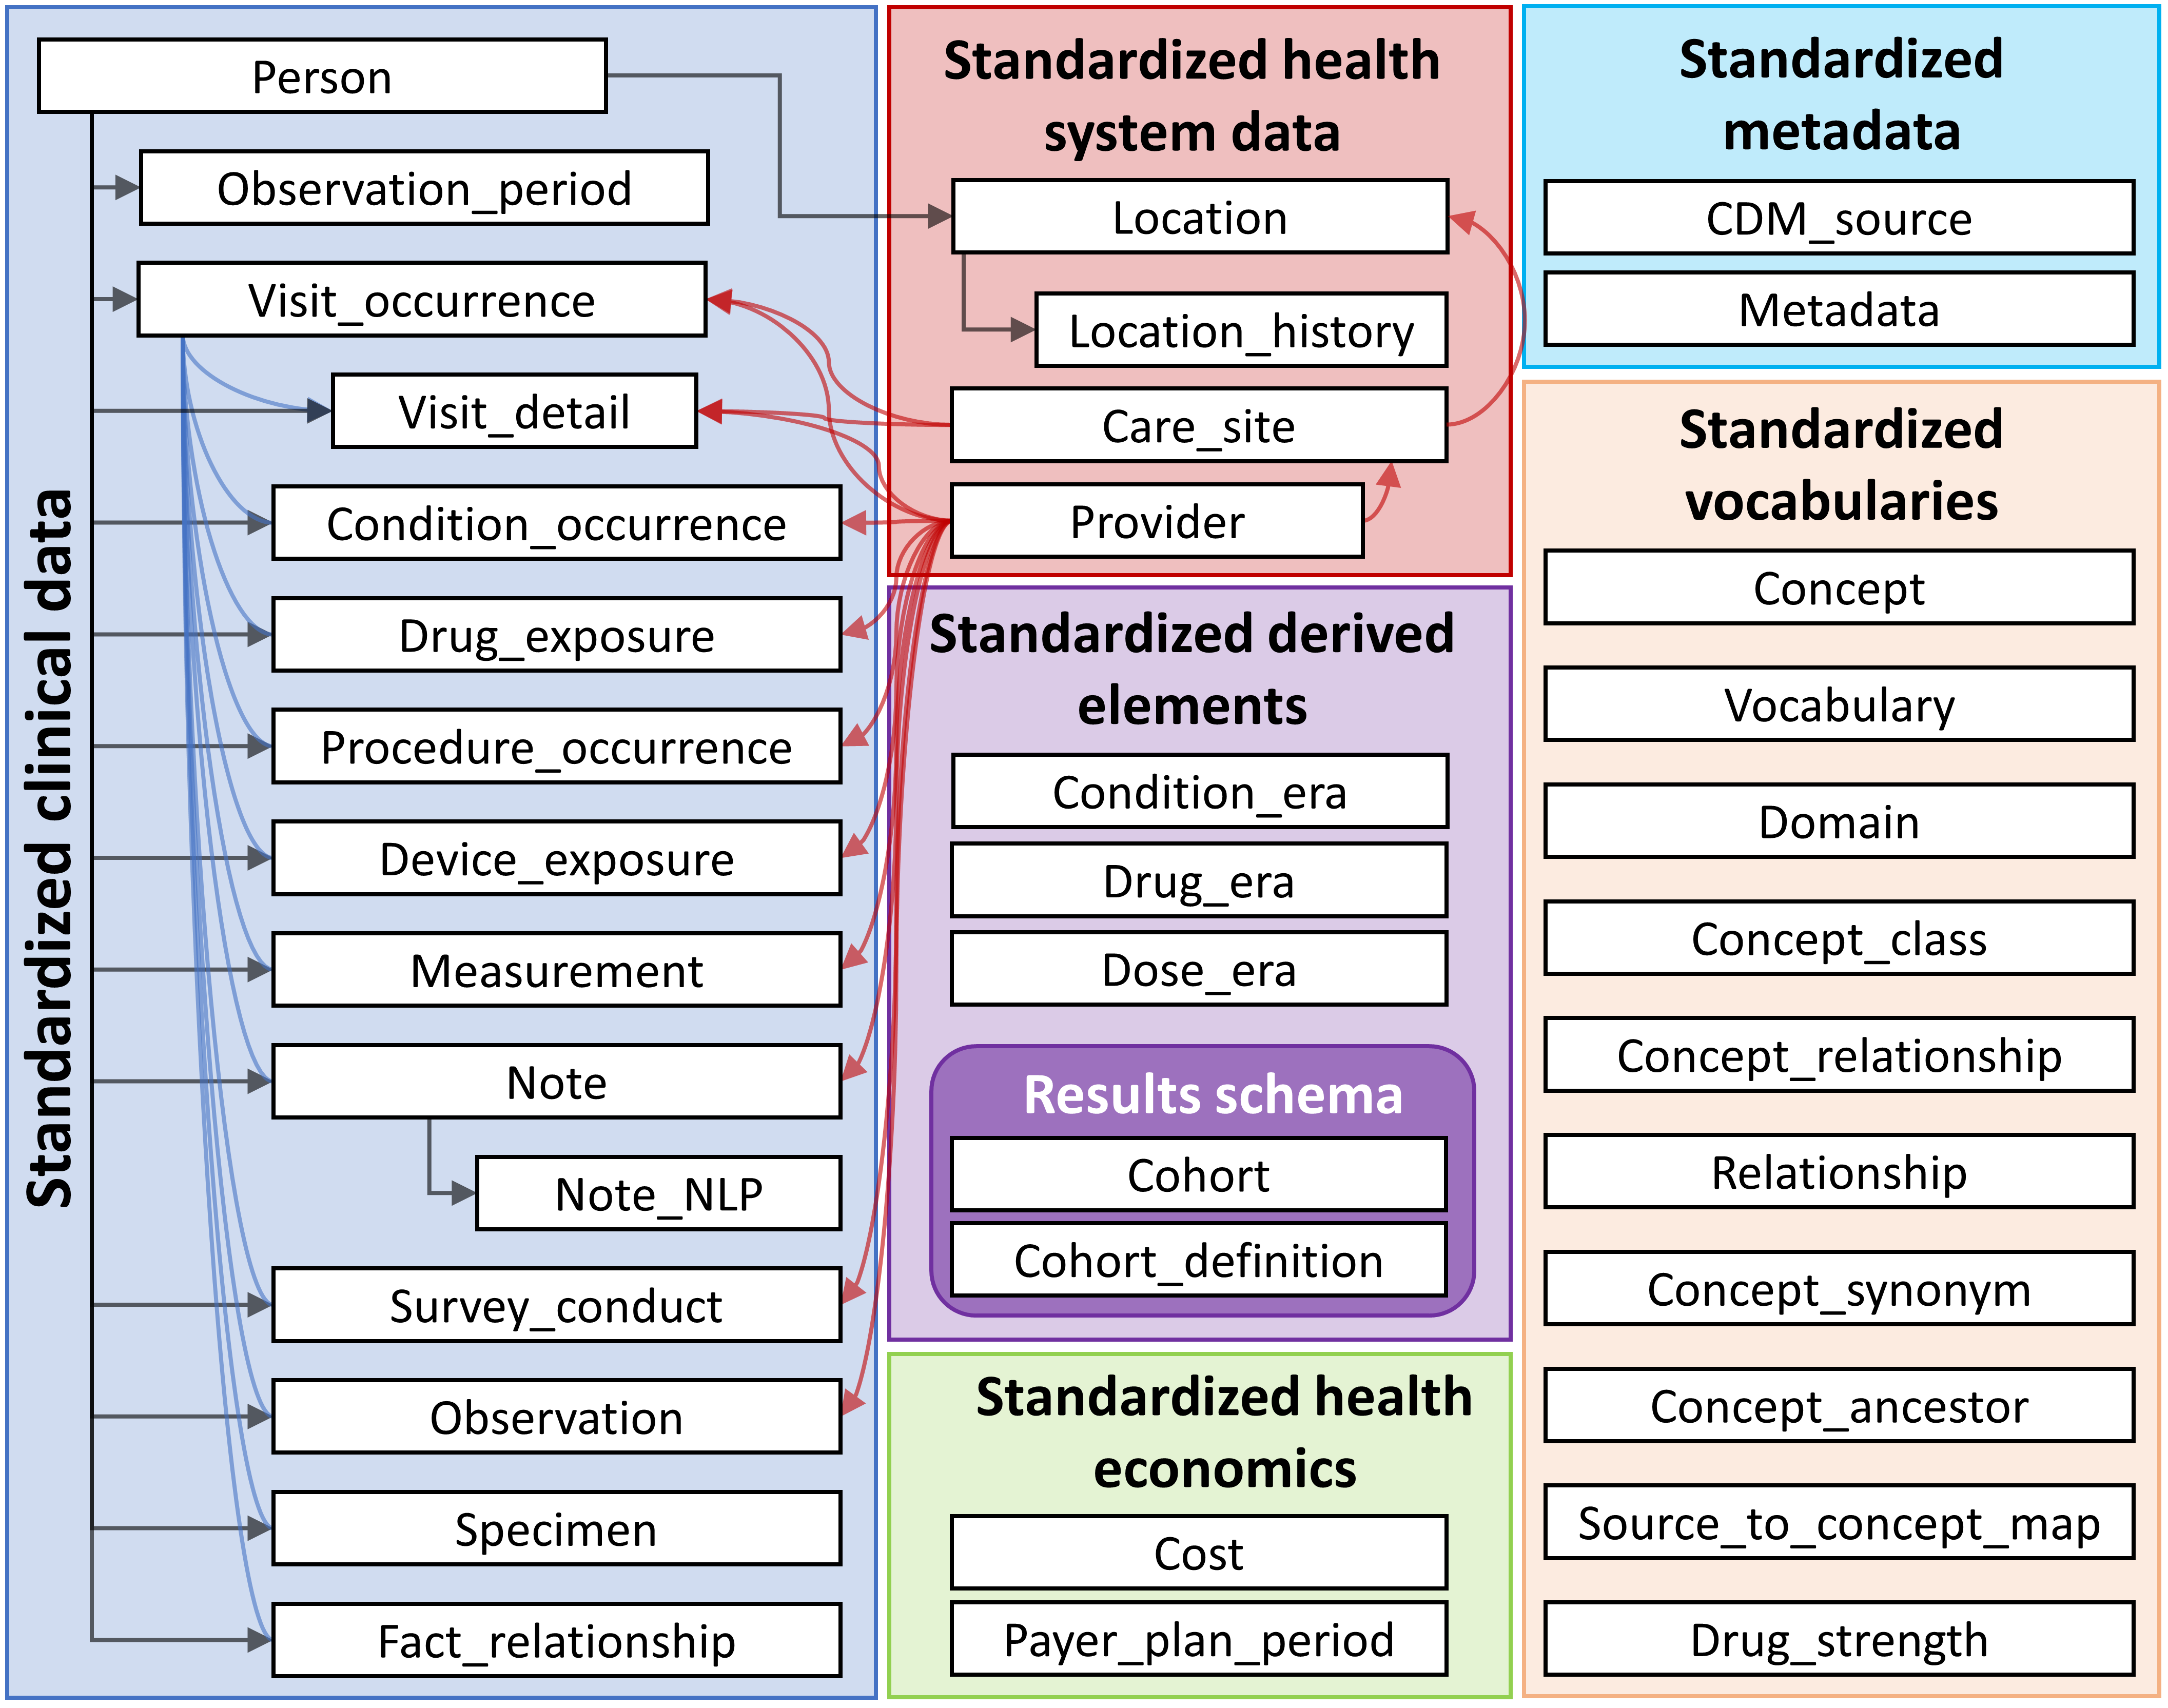
\includegraphics[width=1\linewidth]{images/CommonDataModel/cdmDiagram} \caption{Overview of all tables in the CDM version 6.0. Note that not all relationships between tables are shown.}\label{fig:cdmDiagram}
\end{figure}

\section{Design Principles}\label{design-principles}

The CDM is optimized for typical observational research purposes of
\index{Common Data Model!design principles}

\begin{itemize}
\tightlist
\item
  Identifying patient populations with certain healthcare interventions
  (drug exposure, procedures, healthcare policy changes etc.) and
  outcomes (conditions, procedures, other drug exposures etc.),
\item
  Characterization of these patient populations for various parameters
  like demographic information, disease natural history, healthcare
  delivery, utilization and cost, morbidities, treatments and sequence
  of treatment etc.,
\item
  Predicting the occurrence of these outcomes in individual patients -
  see Chapter \ref{PatientLevelPrediction},
\item
  Estimating the effect these interventions have a population - see
  Chapter \ref{PopulationLevelEstimation},
\end{itemize}

To achieve this goal, the development of the CDM follows the following
design elements:

\begin{itemize}
\tightlist
\item
  \textbf{Suitability for purpose}: The CDM aims to provide data
  organized in a way optimal for analysis, rather than for the purpose
  of addressing the operational needs of health care providers or
  payers. \index{Common Data Model!suitability for purpose}
\item
  \textbf{Data protection}: All data that might jeopardize the identity
  and protection of patients, such as names, precise birthdays etc. are
  limited. Exceptions are possible when the research expressly requires
  more detailed information, such as precise birth dates for the study
  of infants.\index{Common Data Model!data protection}
\item
  \textbf{Design of domains}: The domains are modeled in a
  person-centric relational data model, where for each record the
  identity of the person and a date is captured as a minimum. Here, a
  relational data model is one where the data is represented as a
  collection of tables linked by primary and foreign keys.
\item
  \textbf{Rationale for domains}: Domains are identified and separately
  defined in an entity-relationship model if they have an analysis use
  case (conditions, for example) and the domain has specific attributes
  that are not otherwise applicable. All other data can be preserved as
  an observation in the observation table in an entity-attribute-value
  structure. \index{Common Data Model!domains}
\item
  \textbf{Standardized Vocabularies}: To standardize the content of
  those records, the CDM relies on the Standardized Vocabularies
  containing all necessary and appropriate corresponding standard
  healthcare concepts.
\item
  \textbf{Reuse of existing vocabularies}: If possible, these concepts
  are leveraged from national or industry standardization or vocabulary
  definition organizations or initiatives, such as the National Library
  of Medicine, the Department of Veterans' Affairs, the Center of
  Disease Control and Prevention, etc.
\item
  \textbf{Maintaining source codes}: Even though all codes are mapped to
  the Standardized Vocabularies, the model also stores the original
  source code to ensure no information is lost.
  \index{Common Data Model!Source Codes}
  \index{Common Data Model!data loss prevention}
\item
  \textbf{Technology neutrality}: The CDM does not require a specific
  technology. It can be realized in any relational database, such as
  Oracle, SQL Server etc., or as SAS analytical
  datasets.\index{Common Data Model!technology neutrality}
\item
  \textbf{Scalability}: The CDM is optimized for data processing and
  computational analysis to accommodate data sources that vary in size,
  including databases with up to hundreds of millions of persons and
  billions of clinical observations.
  \index{Common Data Model!scalability}
\item
  \textbf{Backwards compatibility}: All changes from previous CDMs are
  clearly delineated in the github repository
  \href{https://github.com/OHDSI/CommonDataModel}{(https://github.com/OHDSI/CommonDataModel)}.
  Older versions of the CDM can be easily created from the current
  version, and no information is lost that was present previously.
  \index{Common Data Model!backwards compatibility}
\end{itemize}

\section{Data Model Conventions}\label{data-model-conventions}

There are a number of implicit and explicit conventions that have been
adopted in the CDM. Developers of methods that run against the CDM need
to understand these conventions. \index{Common Data Model!conventions}

\subsection{General Conventions of the Model}\label{model-Conv}

The CDM is considered a ``person-centric'' model, meaning that all
clinical Event tables are linked to the PERSON table. Together with the
date or start date this allows for a longitudinal view on all
healthcare-relevant Events by person. The exceptions from this rule are
the standardized health system data tables, which are linked directly to
Events of the various domains.

\subsection{General Conventions of
Schemas}\label{general-conventions-of-schemas}

Schemas, or database users in some systems, allow for separation between
read-only and read-write tables. The clinical Event and vocabulary
tables are in the ``CDM'' schema and are considered read-only to the end
user or analytic tool. Tables that need to be manipulated by web-based
tools or end users are stored in the ``Results'' schema. The two tables
in the ``Results'' schema are COHORT and COHORT\_DEFINITON. These tables
are meant to describe groups of interest that the user might define, as
detailed in Chapter \ref{Cohorts}. These tables can be written to,
meaning that a cohort can be stored in the COHORT table at run time.
Since there is only one read-write schema for all users it is up to the
implementation of the CDM how multiple user access is organized and
controlled.

\subsection{General Conventions of Data
Tables}\label{general-conventions-of-data-tables}

The CDM is platform-independent. Data types are defined generically
using ANSI SQL data types (VARCHAR, INTEGER, FLOAT, DATE, DATETIME,
CLOB). Precision is provided only for VARCHAR. It reflects the minimal
required string length, but can be expanded within a concrete CDM
instantiation. The CDM does not prescribe the date and datetime format.
Standard queries against CDM may vary for local instances and
date/datetime configurations.

\emph{Note}: While the data model itself is platform-independent, many
of the tools that have been built to work with it require certain
specifications. For more about this please see Chapter
\ref{OhdsiAnalyticsTools}.

\subsection{General Conventions of Domains}\label{domains}

Events of different nature are organized into Domains. These Events are
stored in tables and fields which are Domain-specific, and represented
by Standard Concepts that are also Domain-specific as defined in the
Standardized Vocabularies (see section \ref{conceptDomains}). Each
Standard Concept has a unique Domain assignment, which defines which
table they are recorded in. Even though the correct Domain assignment is
subject for debate in the community, this strict Domain-table-field
correspondence rule assures that there is always an unambiguous location
for any code or concept. For example, signs, symptoms and diagnosis
Concepts are of the Condition Domain, and are recorded in the
CONDITION\_CONCEPT\_ID of the CONDITION\_OCCURRENCE table. So-called
Procedure Drugs are typically recorded as procedure codes in a procedure
table in the source data. In an CDM, these records are found in the
DRUG\_EXPOSURE table because the mapped Standard Concepts have the
Domain assignment Drug. There is a total of 30 Domains, as shown in
table \ref{tab:domains}.

\begin{longtable}[]{@{}llll@{}}
\caption{\label{tab:domains} Number of standard concepts belonging to each
domain.}\tabularnewline
\toprule
Concept Count & Domain ID & Concept Count & Domain ID\tabularnewline
\midrule
\endfirsthead
\toprule
Concept Count & Domain ID & Concept Count & Domain ID\tabularnewline
\midrule
\endhead
1731378 & Drug & 183 & Route\tabularnewline
477597 & Device & 180 & Currency\tabularnewline
257000 & Procedure & 158 & Payer\tabularnewline
163807 & Condition & 123 & Visit\tabularnewline
145898 & Observation & 51 & Cost\tabularnewline
89645 & Measurement & 50 & Race\tabularnewline
33759 & Spec Anatomic Site & 13 & Plan Stop Reason\tabularnewline
17302 & Meas Value & 11 & Plan\tabularnewline
1799 & Specimen & 6 & Episode\tabularnewline
1215 & Provider Specialty & 6 & Sponsor\tabularnewline
1046 & Unit & 5 & Meas Value Operator\tabularnewline
944 & Metadata & 3 & Spec Disease Status\tabularnewline
538 & Revenue Code & 2 & Gender\tabularnewline
336 & Type Concept & 2 & Ethnicity\tabularnewline
194 & Relationship & 1 & Observation Type\tabularnewline
\bottomrule
\end{longtable}

\subsection{Representation of Content Through
Concepts}\label{representation-of-content-through-concepts}

In CDM data tables the content of each record is fully normalized and
represented through Concepts. Concepts are stored in Event tables with
their CONCEPT\_ID values, which are foreign keys to the CONCEPT table,
which serves as the general reference table. All CDM instances use the
same CONCEPT table as a reference of the Concepts, which together with
the Common Data Model is a key mechanism of interoperability and the
foundation of the OHDSI research network. If a Standard Concept does not
exist or cannot be identified, the value of the CONCEPT\_ID is set to 0,
representing a non-existing concept, an unknown or un-mappable value.

Records in the CONCEPT table contain detailed information about each
concept (name, domain, class etc.). Concepts, Concept Relationships,
Concept Ancestors and other information relating to Concepts is
contained in the tables of the Standardized Vocabularies (see Chapter
\ref{StandardizedVocabularies}).

\subsection{General Naming Conventions of
Fields}\label{general-naming-conventions-of-fields}

Variable names across all tables follow one convention:

\begin{longtable}[]{@{}ll@{}}
\caption{\label{tab:fieldConventions} Field name
conventions.}\tabularnewline
\toprule
\begin{minipage}[b]{0.34\columnwidth}\raggedright\strut
Notation\strut
\end{minipage} & \begin{minipage}[b]{0.60\columnwidth}\raggedright\strut
Description\strut
\end{minipage}\tabularnewline
\midrule
\endfirsthead
\toprule
\begin{minipage}[b]{0.34\columnwidth}\raggedright\strut
Notation\strut
\end{minipage} & \begin{minipage}[b]{0.60\columnwidth}\raggedright\strut
Description\strut
\end{minipage}\tabularnewline
\midrule
\endhead
\begin{minipage}[t]{0.34\columnwidth}\raggedright\strut
{[}Event{]}\_ID\strut
\end{minipage} & \begin{minipage}[t]{0.60\columnwidth}\raggedright\strut
Unique identifier for each record, which serves as a foreign keys
establishing relationships across Event tables. For example, PERSON\_ID
uniquely identifies each individual. VISIT\_OCCURRENCE\_ID uniquely
identifies a Visit.\strut
\end{minipage}\tabularnewline
\begin{minipage}[t]{0.34\columnwidth}\raggedright\strut
{[}Event{]}\_CONCEPT\_ID\strut
\end{minipage} & \begin{minipage}[t]{0.60\columnwidth}\raggedright\strut
Foreign key to a Standard Concept record in the CONCEPT reference table.
This is the main representation of the Event, serving as the primary
basis for all standardized analytics. For example,
CONDITION\_CONCEPT\_ID =
\href{http://athena.ohdsi.org/search-terms/terms/31967}{31967} contains
the reference value for the SNOMED concept of ``Nausea''.\strut
\end{minipage}\tabularnewline
\begin{minipage}[t]{0.34\columnwidth}\raggedright\strut
{[}Event{]}\_SOURCE \_CONCEPT\_ID\strut
\end{minipage} & \begin{minipage}[t]{0.60\columnwidth}\raggedright\strut
Foreign key to a record in the CONCEPT reference table. This Concept is
the equivalent of the Source Value (below), and it may happen to be a
Standard Concept, at which point it would be identical to the
{[}Event{]}\_CONCEPT\_ID, or another non-standard concept. For example,
CONDITION\_SOURCE\_CONCEPT\_ID =
\href{http://athena.ohdsi.org/search-terms/terms/45431665}{45431665}
denotes the concept of ``Nausea'' in the Read terminology, and the
analogous CONDITION\_CONCEPT\_ID is the Standard SNOMED-CT Concept
\href{http://athena.ohdsi.org/search-terms/terms/31967}{31967}. The use
of Source Concepts for standard analytics applications is discouraged
since only Standard Concepts represent the semantic content of an Event
in a unambiguous way and therefore Source Concepts are not
interoperable.\strut
\end{minipage}\tabularnewline
\begin{minipage}[t]{0.34\columnwidth}\raggedright\strut
{[}Event{]}\_TYPE\_CONCEPT\_ID\strut
\end{minipage} & \begin{minipage}[t]{0.60\columnwidth}\raggedright\strut
Foreign key to a record in the CONCEPT reference table, representing the
origin of the source information, standardized within the Standardized
Vocabularies. Note that despite the field name this is not a type of an
Event, or type of a Concept, but declares the capture mechanism that
created this record. For example, DRUG\_TYPE\_CONCEPT\_ID discriminates
if a Drug record was derived from a dispensing Event in the pharmacy
(``Pharmacy dispensing'') or from an e-prescribing application
(``Prescription written'')\strut
\end{minipage}\tabularnewline
\begin{minipage}[t]{0.34\columnwidth}\raggedright\strut
{[}Event{]}\_SOURCE\_VALUE\strut
\end{minipage} & \begin{minipage}[t]{0.60\columnwidth}\raggedright\strut
Verbatim code or free text string reflecting how this Event was
represented in the source data. Its use is discouraged for standard
analytics applications, as these Source Values are not harmonized across
data sources. For example, CONDITION\_SOURCE\_VALUE might contain a
record of ``78702'', corresponding to ICD-9 code 787.02 written in a
notation omitting the dot.\strut
\end{minipage}\tabularnewline
\bottomrule
\end{longtable}

\subsection{Difference Between Concepts and Source
Values}\label{concepts-Sources}

Many tables contain equivalent information in multiple places: as a
Source Value, a Source Concept and as a Standard Concept.

\begin{itemize}
\tightlist
\item
  \textbf{Source Values} are the original representation of an Event
  record in the source data. They can be codes from widely used coding
  systems, which are often public domain, such as ICD9CM, NDC or Read,
  proprietary coding systems like CPT4, GPI or MedDRA, or controlled
  vocabularies used only in the source data, such as F for female and M
  for male. They can also be short free text phrases that are not
  standardized and controlled. Source Values are stored in the
  {[}Event{]}\_SOURCE\_VALUE fields in the data tables.
\item
  \textbf{Concepts} are CDM-specific entities that normalize the meaning
  of a clinical fact. Most Concepts are based on existing public or
  proprietary coding systems in healthcare, while others were created
  de-novo (CONCEPT\_CODE starts with ``OMOP''). Concepts have unique IDs
  across all domains.
\item
  \textbf{Source Concepts} are the Concepts that represent the code used
  in the source. Source Concepts are only used for existing public or
  proprietary coding systems, not for OMOP-generated Concepts. Source
  Concepts are stored in the {[}Event{]}\_SOURCE\_CONCEPT\_ID field in
  the data tables.
\item
  \textbf{Standard Concepts} are those Concepts that are used to define
  the meaning of a clinical entity uniquely across all databases and
  independent from the coding system used in the sources. Standard
  Concepts are typically drawn from existing public or proprietary
  vocabulary sources. Non-standard Concepts that have the equivalent
  meaning to a Standard Concept have a mapping to the Standard Concept
  in the Standardized Vocabularies. Standard Concepts are referred to in
  the {[}Event{]}\_CONCEPT\_ID field of the data tables.
\end{itemize}

Source Values are only provided for convenience and quality assurance
(QA) purposes. They may contain information that is only meaningful in
the context of a specific data source. The use of Source Values and
Source Concepts is optional, even though \textbf{strongly recommended}
if the source data make use of coding systems. Standard Concepts
\textbf{are mandatory} however. This mandatory use of Standard Concepts
is what allows all CDM instances to speak the same language. For
example, the condition ``Pulmonary Tuberculosis'' (TB, Figure
\ref{fig:pulmTubICD9}) shows that the ICD9CM code for TB is 011.

\begin{figure}

{\centering 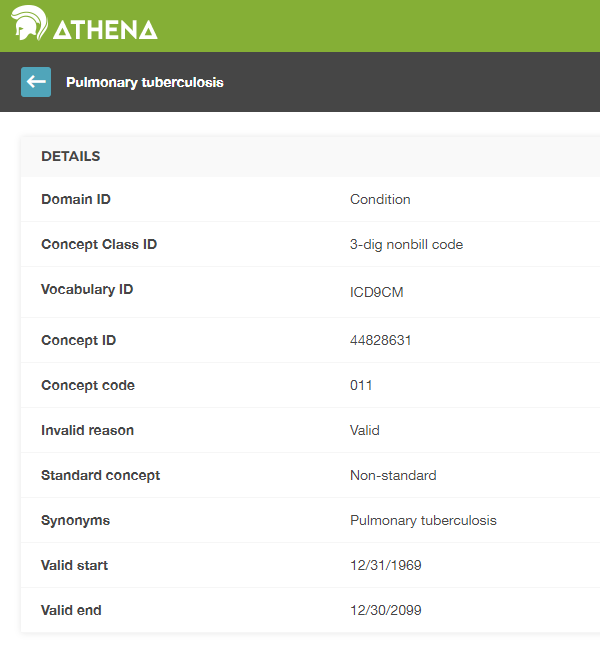
\includegraphics[width=0.75\linewidth]{images/CommonDataModel/pulmTubICD9} 

}

\caption{ICD9CM code for Pulmonary Tuberculosis}\label{fig:pulmTubICD9}
\end{figure}

Without context, the code 011 could be interpreted as ``Hospital
Inpatient (Including Medicare Part A)'' from the UB04 vocabulary, or as
``Nervous System Neoplasms without Complications, Comorbidities'' from
the DRG vocabulary. This is where Concept IDs, both Source and Standard,
are valuable. The CONCEPT\_ID value that represents the 011 ICD9CM code
is \href{http://athena.ohdsi.org/search-terms/terms/44828631}{44828631}.
This differentiates the ICD9CM from the UBO4 and DRG. The ICD9CM TB
Source Concept maps to Standard Concept
\href{http://athena.ohdsi.org/search-terms/terms/253954}{253954} from
the SNOMED vocabulary through the relationship ``Non-standard to
Standard map (OMOP)'' as shown in figure \ref{fig:pulmTubMap}. This same
mapping relationships exists for Read, ICD10, CIEL, and MeSH codes,
among others, so that any research that references the standard SNOMED
concept is sure to include all supported source codes.

\begin{figure}
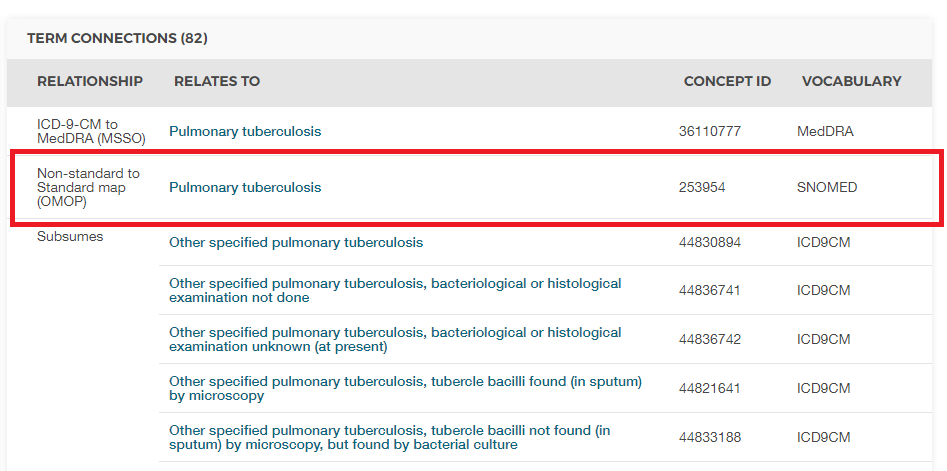
\includegraphics[width=1\linewidth]{images/CommonDataModel/pulmTubMap} \caption{SNOMED code for Pulmonary Tuberculosis}\label{fig:pulmTubMap}
\end{figure}

An example of how the Standard Concept to Source Concept relationship is
depicted is shown in Table \ref{tab:conditionOccurrence}.

\section{CDM Standardized Tables}\label{cdm-standardized-tables}

\index{Common Data Model!standardized tables}

The CDM contains 16 Clinical Event tables, 10 Vocabulary tables, 2
metadata tables, 4 health system data tables, 2 health economics data
tables, 3 standardized derived elements, and 2 Results schema tables.
These tables are fully specified in the CDM Wiki.\footnote{\url{https://github.com/OHDSI/CommonDataModel/wiki}}

To illustrate how these tables are used in practice, the data of one
person will be used as a common thread throughout the rest of the
chapter.

\subsection{Running Example:
Endometriosis}\label{running-example-endometriosis}

Endometriosis is a painful condition whereby cells normally found in the
lining of a woman's uterus occur elsewhere in the body. Severe cases can
lead to infertility, bowel, and bladder problems. The following sections
will detail one patient's experience with this disease and how it might
be represented in the Common Data Model.

\begin{center}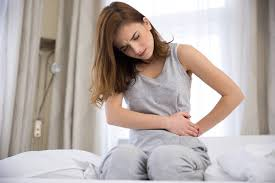
\includegraphics[width=0.5\linewidth]{images/CommonDataModel/Lauren} \end{center}

\begin{quote}
Every step of this painful journey I had to convince everyone how much
pain I was in.
\end{quote}

Lauren had been experiencing endometriosis symptoms for many years;
however, it took a ruptured cyst in her ovary before she was diagnosed.
You can read more about Lauren at
\url{https://www.endometriosis-uk.org/laurens-story}.

\subsection{PERSON Table}\label{person}

\subsubsection*{What Do We Know About
Lauren?}\label{what-do-we-know-about-lauren}
\addcontentsline{toc}{subsubsection}{What Do We Know About Lauren?}

\begin{itemize}
\tightlist
\item
  She is a 36-year-old woman
\item
  Her birthday is 12-March-1982
\item
  She is white
\item
  She is English
\end{itemize}

With that in mind, her PERSON table might look something like this:

\begin{longtable}[]{@{}lll@{}}
\caption{\label{tab:person} The PERSON table.}\tabularnewline
\toprule
\begin{minipage}[b]{0.28\columnwidth}\raggedright\strut
Column name\strut
\end{minipage} & \begin{minipage}[b]{0.16\columnwidth}\raggedright\strut
Value\strut
\end{minipage} & \begin{minipage}[b]{0.48\columnwidth}\raggedright\strut
Explanation\strut
\end{minipage}\tabularnewline
\midrule
\endfirsthead
\toprule
\begin{minipage}[b]{0.28\columnwidth}\raggedright\strut
Column name\strut
\end{minipage} & \begin{minipage}[b]{0.16\columnwidth}\raggedright\strut
Value\strut
\end{minipage} & \begin{minipage}[b]{0.48\columnwidth}\raggedright\strut
Explanation\strut
\end{minipage}\tabularnewline
\midrule
\endhead
\begin{minipage}[t]{0.28\columnwidth}\raggedright\strut
PERSON\_ID\strut
\end{minipage} & \begin{minipage}[t]{0.16\columnwidth}\raggedright\strut
1\strut
\end{minipage} & \begin{minipage}[t]{0.48\columnwidth}\raggedright\strut
The PERSON\_ID should be an integer, either directly from the source or
generated as part of the build process.\strut
\end{minipage}\tabularnewline
\begin{minipage}[t]{0.28\columnwidth}\raggedright\strut
GENDER\_CONCEPT\_ID\strut
\end{minipage} & \begin{minipage}[t]{0.16\columnwidth}\raggedright\strut
8532\strut
\end{minipage} & \begin{minipage}[t]{0.48\columnwidth}\raggedright\strut
The concept ID referring to female gender is
\href{http://athena.ohdsi.org/search-terms/terms/8532}{8532}.\strut
\end{minipage}\tabularnewline
\begin{minipage}[t]{0.28\columnwidth}\raggedright\strut
YEAR\_OF\_BIRTH\strut
\end{minipage} & \begin{minipage}[t]{0.16\columnwidth}\raggedright\strut
1982\strut
\end{minipage} & \begin{minipage}[t]{0.48\columnwidth}\raggedright\strut
\strut
\end{minipage}\tabularnewline
\begin{minipage}[t]{0.28\columnwidth}\raggedright\strut
MONTH\_OF\_BIRTH\strut
\end{minipage} & \begin{minipage}[t]{0.16\columnwidth}\raggedright\strut
3\strut
\end{minipage} & \begin{minipage}[t]{0.48\columnwidth}\raggedright\strut
\strut
\end{minipage}\tabularnewline
\begin{minipage}[t]{0.28\columnwidth}\raggedright\strut
DAY\_OF\_BIRTH\strut
\end{minipage} & \begin{minipage}[t]{0.16\columnwidth}\raggedright\strut
12\strut
\end{minipage} & \begin{minipage}[t]{0.48\columnwidth}\raggedright\strut
\strut
\end{minipage}\tabularnewline
\begin{minipage}[t]{0.28\columnwidth}\raggedright\strut
BIRTH\_DATETIME\strut
\end{minipage} & \begin{minipage}[t]{0.16\columnwidth}\raggedright\strut
1982-03-12 00:00:00\strut
\end{minipage} & \begin{minipage}[t]{0.48\columnwidth}\raggedright\strut
When the time is not known midnight is used.\strut
\end{minipage}\tabularnewline
\begin{minipage}[t]{0.28\columnwidth}\raggedright\strut
DEATH\_DATETIME\strut
\end{minipage} & \begin{minipage}[t]{0.16\columnwidth}\raggedright\strut
\strut
\end{minipage} & \begin{minipage}[t]{0.48\columnwidth}\raggedright\strut
\strut
\end{minipage}\tabularnewline
\begin{minipage}[t]{0.28\columnwidth}\raggedright\strut
RACE\_CONCEPT\_ID\strut
\end{minipage} & \begin{minipage}[t]{0.16\columnwidth}\raggedright\strut
8527\strut
\end{minipage} & \begin{minipage}[t]{0.48\columnwidth}\raggedright\strut
The concept ID referring to white race is
\href{http://athena.ohdsi.org/search-terms/terms/8527}{8527}. English
ethnicity is
\href{http://athena.ohdsi.org/search-terms/terms/4093769}{4093769}.
Either one is correct, the latter will roll up to the former. Notice
that ethnicities are stored here as part of Races, not in the
ETHNICITY\_CONCEPT\_ID\strut
\end{minipage}\tabularnewline
\begin{minipage}[t]{0.28\columnwidth}\raggedright\strut
ETHNICITY\_CONCEPT\_ ID\strut
\end{minipage} & \begin{minipage}[t]{0.16\columnwidth}\raggedright\strut
38003564\strut
\end{minipage} & \begin{minipage}[t]{0.48\columnwidth}\raggedright\strut
This is a US-typical notation to distinguish Hispanics from the rest.
Ethnicities, in this case English, is stored in the RACE\_CONCEPT\_ID.
Outside the US this is not used.
\href{http://athena.ohdsi.org/search-terms/terms/38003564}{38003564}
refers to ``Not hispanic''.\strut
\end{minipage}\tabularnewline
\begin{minipage}[t]{0.28\columnwidth}\raggedright\strut
LOCATION\_ID\strut
\end{minipage} & \begin{minipage}[t]{0.16\columnwidth}\raggedright\strut
\strut
\end{minipage} & \begin{minipage}[t]{0.48\columnwidth}\raggedright\strut
Her address is not known.\strut
\end{minipage}\tabularnewline
\begin{minipage}[t]{0.28\columnwidth}\raggedright\strut
PROVIDER\_ID\strut
\end{minipage} & \begin{minipage}[t]{0.16\columnwidth}\raggedright\strut
\strut
\end{minipage} & \begin{minipage}[t]{0.48\columnwidth}\raggedright\strut
Her primary care Provider is not known.\strut
\end{minipage}\tabularnewline
\begin{minipage}[t]{0.28\columnwidth}\raggedright\strut
CARE\_SITE\strut
\end{minipage} & \begin{minipage}[t]{0.16\columnwidth}\raggedright\strut
\strut
\end{minipage} & \begin{minipage}[t]{0.48\columnwidth}\raggedright\strut
Her primary Care Site is not known.\strut
\end{minipage}\tabularnewline
\begin{minipage}[t]{0.28\columnwidth}\raggedright\strut
PERSON\_SOURCE\_ VALUE\strut
\end{minipage} & \begin{minipage}[t]{0.16\columnwidth}\raggedright\strut
1\strut
\end{minipage} & \begin{minipage}[t]{0.48\columnwidth}\raggedright\strut
Typically this would be her identifier in the source data, though often
it is the same as the PERSON\_ID.\strut
\end{minipage}\tabularnewline
\begin{minipage}[t]{0.28\columnwidth}\raggedright\strut
GENDER\_SOURCE\_ VALUE\strut
\end{minipage} & \begin{minipage}[t]{0.16\columnwidth}\raggedright\strut
F\strut
\end{minipage} & \begin{minipage}[t]{0.48\columnwidth}\raggedright\strut
The gender value as it appears in the source is stored here.\strut
\end{minipage}\tabularnewline
\begin{minipage}[t]{0.28\columnwidth}\raggedright\strut
GENDER\_SOURCE\_ CONCEPT\_ID\strut
\end{minipage} & \begin{minipage}[t]{0.16\columnwidth}\raggedright\strut
0\strut
\end{minipage} & \begin{minipage}[t]{0.48\columnwidth}\raggedright\strut
If the gender value in the source was coded using a coding scheme
supported by OHDSI that Concept would go here. For example, if her
gender was ``sex-F'' in the source and it was stated to be in the
PCORNet vocabulary concept
\href{http://athena.ohdsi.org/search-terms/terms/44814665}{44814665}
would go in this field.\strut
\end{minipage}\tabularnewline
\begin{minipage}[t]{0.28\columnwidth}\raggedright\strut
RACE\_SOURCE\_ VALUE\strut
\end{minipage} & \begin{minipage}[t]{0.16\columnwidth}\raggedright\strut
white\strut
\end{minipage} & \begin{minipage}[t]{0.48\columnwidth}\raggedright\strut
The race value as it appears in the source is stored here.\strut
\end{minipage}\tabularnewline
\begin{minipage}[t]{0.28\columnwidth}\raggedright\strut
RACE\_SOURCE\_ CONCEPT\_ID\strut
\end{minipage} & \begin{minipage}[t]{0.16\columnwidth}\raggedright\strut
0\strut
\end{minipage} & \begin{minipage}[t]{0.48\columnwidth}\raggedright\strut
Same principle as GENDER\_CONCEPT\_ID.\strut
\end{minipage}\tabularnewline
\begin{minipage}[t]{0.28\columnwidth}\raggedright\strut
ETHNICITY\_SOURCE\_ VALUE\strut
\end{minipage} & \begin{minipage}[t]{0.16\columnwidth}\raggedright\strut
english\strut
\end{minipage} & \begin{minipage}[t]{0.48\columnwidth}\raggedright\strut
The ethnicity value as it appears in the source is stored here.\strut
\end{minipage}\tabularnewline
\begin{minipage}[t]{0.28\columnwidth}\raggedright\strut
ETHNICITY\_SOURCE\_ CONCEPT\_ID\strut
\end{minipage} & \begin{minipage}[t]{0.16\columnwidth}\raggedright\strut
0\strut
\end{minipage} & \begin{minipage}[t]{0.48\columnwidth}\raggedright\strut
Same principle as GENDER\_SOURCE\_CONCEPT\_ID.\strut
\end{minipage}\tabularnewline
\bottomrule
\end{longtable}

\subsection{OBSERVATION\_PERIOD Table}\label{observationPeriod}

The OBSERVATION\_PERIOD table is designed to define the amount of time
for which at least a patient's demographics, conditions, procedures and
drugs are recorded in the source system with the expectation of a
reasonable sensitivity and specificity. For insurance data this is
typically the enrollment period of the patient. It's trickier in
electronic health records (EHR), as most healthcare systems do not
determine which healthcare institution or provider is visited. As a next
best solution, often the first record in the system is considered the
Start Date of the Observation Period and the latest record is considered
the End Date.

\subsubsection*{How Is Lauren's Observation Period
Defined?}\label{how-is-laurens-observation-period-defined}
\addcontentsline{toc}{subsubsection}{How Is Lauren's Observation Period
Defined?}

Let's say Lauren's information as shown in Table \ref{tab:encounters} is
recorded like in an EHR system. Her encounters from which the
Observation Period was derived are:

\begin{longtable}[]{@{}llll@{}}
\caption{\label{tab:encounters} Lauren's healthcare
encounters.}\tabularnewline
\toprule
Encounter ID & Start date & Stop date & Type\tabularnewline
\midrule
\endfirsthead
\toprule
Encounter ID & Start date & Stop date & Type\tabularnewline
\midrule
\endhead
70 & 2010-01-06 & 2010-01-06 & outpatient\tabularnewline
80 & 2011-01-06 & 2011-01-06 & outpatient\tabularnewline
90 & 2012-01-06 & 2012-01-06 & outpatient\tabularnewline
100 & 2013-01-07 & 2013-01-07 & outpatient\tabularnewline
101 & 2013-01-14 & 2013-01-14 & ambulatory\tabularnewline
102 & 2013-01-17 & 2013-01-24 & inpatient\tabularnewline
\bottomrule
\end{longtable}

Based on the encounter records her OBSERVATION\_PERIOD table might look
something like this:

\begin{longtable}[]{@{}lll@{}}
\caption{\label{tab:observationPeriod} The OBSERVATION\_PERIOD
table.}\tabularnewline
\toprule
\begin{minipage}[b]{0.29\columnwidth}\raggedright\strut
Column name\strut
\end{minipage} & \begin{minipage}[b]{0.14\columnwidth}\raggedright\strut
Value\strut
\end{minipage} & \begin{minipage}[b]{0.48\columnwidth}\raggedright\strut
Explanation\strut
\end{minipage}\tabularnewline
\midrule
\endfirsthead
\toprule
\begin{minipage}[b]{0.29\columnwidth}\raggedright\strut
Column name\strut
\end{minipage} & \begin{minipage}[b]{0.14\columnwidth}\raggedright\strut
Value\strut
\end{minipage} & \begin{minipage}[b]{0.48\columnwidth}\raggedright\strut
Explanation\strut
\end{minipage}\tabularnewline
\midrule
\endhead
\begin{minipage}[t]{0.29\columnwidth}\raggedright\strut
OBSERVATION\_ PERIOD\_ID\strut
\end{minipage} & \begin{minipage}[t]{0.14\columnwidth}\raggedright\strut
1\strut
\end{minipage} & \begin{minipage}[t]{0.48\columnwidth}\raggedright\strut
This is typically an autogenerated value creating a unique identifier
for each record in the table.\strut
\end{minipage}\tabularnewline
\begin{minipage}[t]{0.29\columnwidth}\raggedright\strut
PERSON\_ID\strut
\end{minipage} & \begin{minipage}[t]{0.14\columnwidth}\raggedright\strut
1\strut
\end{minipage} & \begin{minipage}[t]{0.48\columnwidth}\raggedright\strut
This is a foreign key to Laura's record in the PERSON table and links
PERSON to OBSERVATION\_PERIOD table.\strut
\end{minipage}\tabularnewline
\begin{minipage}[t]{0.29\columnwidth}\raggedright\strut
OBSERVATION\_PERIOD\_ START\_DATE\strut
\end{minipage} & \begin{minipage}[t]{0.14\columnwidth}\raggedright\strut
2010-01-06\strut
\end{minipage} & \begin{minipage}[t]{0.48\columnwidth}\raggedright\strut
This is the start date of her earliest encounter on record.\strut
\end{minipage}\tabularnewline
\begin{minipage}[t]{0.29\columnwidth}\raggedright\strut
OBSERVATION\_PERIOD\_ END\_DATE\strut
\end{minipage} & \begin{minipage}[t]{0.14\columnwidth}\raggedright\strut
2013-01-24\strut
\end{minipage} & \begin{minipage}[t]{0.48\columnwidth}\raggedright\strut
This is the end date of her latest encounter on record.\strut
\end{minipage}\tabularnewline
\begin{minipage}[t]{0.29\columnwidth}\raggedright\strut
PERIOD\_TYPE\_ CONCEPT\_ID\strut
\end{minipage} & \begin{minipage}[t]{0.14\columnwidth}\raggedright\strut
44814725\strut
\end{minipage} & \begin{minipage}[t]{0.48\columnwidth}\raggedright\strut
The best option in the Vocabulary with the concept class ``Obs Period
Type'' is
\href{http://athena.ohdsi.org/search-terms/terms/44814724}{44814724},
which stands for ``Period covering healthcare encounters''.\strut
\end{minipage}\tabularnewline
\bottomrule
\end{longtable}

\subsection{VISIT\_OCCURRENCE}\label{visitOccurrence}

the VISIT\_OCCURRENCE table houses information about a patient's
encounters with the health care system. Within the OHDSI vernacular
these are referred to as Visits and are considered to be discreet
events. There are 12 top categories of Visits with an extensive
hierarchy, depicting the many different circumstances healthcare might
be delivered. The most common Visits recorded are inpatient, outpatient,
emergency department and non-medical institution Visits.

\subsubsection*{How Are Lauren's Encounters Represented As
Visits?}\label{how-are-laurens-encounters-represented-as-visits}
\addcontentsline{toc}{subsubsection}{How Are Lauren's Encounters
Represented As Visits?}

As an example let's represent the inpatient encounter in Table
\ref{tab:encounters} in the VISIT\_OCCURRENCE table.

\begin{longtable}[]{@{}lll@{}}
\caption{\label{tab:visitOccurrence} the VISIT\_OCCURRENCE
table.}\tabularnewline
\toprule
\begin{minipage}[b]{0.28\columnwidth}\raggedright\strut
Column name\strut
\end{minipage} & \begin{minipage}[b]{0.16\columnwidth}\raggedright\strut
Value\strut
\end{minipage} & \begin{minipage}[b]{0.48\columnwidth}\raggedright\strut
Explanation\strut
\end{minipage}\tabularnewline
\midrule
\endfirsthead
\toprule
\begin{minipage}[b]{0.28\columnwidth}\raggedright\strut
Column name\strut
\end{minipage} & \begin{minipage}[b]{0.16\columnwidth}\raggedright\strut
Value\strut
\end{minipage} & \begin{minipage}[b]{0.48\columnwidth}\raggedright\strut
Explanation\strut
\end{minipage}\tabularnewline
\midrule
\endhead
\begin{minipage}[t]{0.28\columnwidth}\raggedright\strut
VISIT\_OCCURRENCE\_ ID\strut
\end{minipage} & \begin{minipage}[t]{0.16\columnwidth}\raggedright\strut
514\strut
\end{minipage} & \begin{minipage}[t]{0.48\columnwidth}\raggedright\strut
This is typically an autogenerated value creating a unique identifier
for each record.\strut
\end{minipage}\tabularnewline
\begin{minipage}[t]{0.28\columnwidth}\raggedright\strut
PERSON\_ID\strut
\end{minipage} & \begin{minipage}[t]{0.16\columnwidth}\raggedright\strut
1\strut
\end{minipage} & \begin{minipage}[t]{0.48\columnwidth}\raggedright\strut
This is a foreign key to Laura's record in the PERSON table and links
PERSON to VISIT\_OCCURRENCE.\strut
\end{minipage}\tabularnewline
\begin{minipage}[t]{0.28\columnwidth}\raggedright\strut
VISIT\_CONCEPT\_ID\strut
\end{minipage} & \begin{minipage}[t]{0.16\columnwidth}\raggedright\strut
9201\strut
\end{minipage} & \begin{minipage}[t]{0.48\columnwidth}\raggedright\strut
A foreign key referring to an Inpatient Visit is
\href{http://athena.ohdsi.org/search-terms/terms/9201}{9201}.\strut
\end{minipage}\tabularnewline
\begin{minipage}[t]{0.28\columnwidth}\raggedright\strut
VISIT\_START\_DATE\strut
\end{minipage} & \begin{minipage}[t]{0.16\columnwidth}\raggedright\strut
2013-01-17\strut
\end{minipage} & \begin{minipage}[t]{0.48\columnwidth}\raggedright\strut
The start date of the Visit.\strut
\end{minipage}\tabularnewline
\begin{minipage}[t]{0.28\columnwidth}\raggedright\strut
VISIT\_START\_ DATETIME\strut
\end{minipage} & \begin{minipage}[t]{0.16\columnwidth}\raggedright\strut
2013-01-17 00:00:00\strut
\end{minipage} & \begin{minipage}[t]{0.48\columnwidth}\raggedright\strut
The date and time of the Visit. The time is unknown, so midnight is
used.\strut
\end{minipage}\tabularnewline
\begin{minipage}[t]{0.28\columnwidth}\raggedright\strut
VISIT\_END\_DATE\strut
\end{minipage} & \begin{minipage}[t]{0.16\columnwidth}\raggedright\strut
2013-01-24\strut
\end{minipage} & \begin{minipage}[t]{0.48\columnwidth}\raggedright\strut
The end date of the Visit. If this is a one-day Visit the end date
should match the start date.\strut
\end{minipage}\tabularnewline
\begin{minipage}[t]{0.28\columnwidth}\raggedright\strut
VISIT\_END\_DATETIME\strut
\end{minipage} & \begin{minipage}[t]{0.16\columnwidth}\raggedright\strut
2013-01-24 00:00:00\strut
\end{minipage} & \begin{minipage}[t]{0.48\columnwidth}\raggedright\strut
The date and time of the Visit end. The time is unknown, so midnight is
used.\strut
\end{minipage}\tabularnewline
\begin{minipage}[t]{0.28\columnwidth}\raggedright\strut
VISIT\_TYPE\_ CONCEPT\_ID\strut
\end{minipage} & \begin{minipage}[t]{0.16\columnwidth}\raggedright\strut
32034\strut
\end{minipage} & \begin{minipage}[t]{0.48\columnwidth}\raggedright\strut
This provides information about the provenance of the Visit record,
i.e.~does it come from an insurance claim, hospital billing, EHR record,
etc. For this example the concept ID
\href{http://athena.ohdsi.org/search-terms/terms/32035}{32035} (``Visit
derived from EHR encounter record'') is used as the encounters are
similar to Electronic Health Records\strut
\end{minipage}\tabularnewline
\begin{minipage}[t]{0.28\columnwidth}\raggedright\strut
PROVIDER\_ID*\strut
\end{minipage} & \begin{minipage}[t]{0.16\columnwidth}\raggedright\strut
NULL\strut
\end{minipage} & \begin{minipage}[t]{0.48\columnwidth}\raggedright\strut
If the encounter record has a provider associated the ID for that
provider goes into this field. This should be the content of the
PROVIDER\_ID field from the PROVIDER table.\strut
\end{minipage}\tabularnewline
\begin{minipage}[t]{0.28\columnwidth}\raggedright\strut
CARE\_SITE\_ID\strut
\end{minipage} & \begin{minipage}[t]{0.16\columnwidth}\raggedright\strut
NULL\strut
\end{minipage} & \begin{minipage}[t]{0.48\columnwidth}\raggedright\strut
If the encounter record has a Care Site associated, the ID for that Care
Site goes into this field. This should be the CARE\_SITE\_ID from the
CARE\_SITE table.\strut
\end{minipage}\tabularnewline
\begin{minipage}[t]{0.28\columnwidth}\raggedright\strut
VISIT\_SOURCE\_ VALUE\strut
\end{minipage} & \begin{minipage}[t]{0.16\columnwidth}\raggedright\strut
inpatient\strut
\end{minipage} & \begin{minipage}[t]{0.48\columnwidth}\raggedright\strut
The Visit value as it appears in the source goes here. Lauren's data do
not have that.\strut
\end{minipage}\tabularnewline
\begin{minipage}[t]{0.28\columnwidth}\raggedright\strut
VISIT\_SOURCE\_ CONCEPT\_ID\strut
\end{minipage} & \begin{minipage}[t]{0.16\columnwidth}\raggedright\strut
0\strut
\end{minipage} & \begin{minipage}[t]{0.48\columnwidth}\raggedright\strut
If the Visit value from the source is coded using a vocabulary that is
recognized by OHDSI the CONCEPT\_ID value representing the source code
would be found here. Lauren's data do not have that.\strut
\end{minipage}\tabularnewline
\begin{minipage}[t]{0.28\columnwidth}\raggedright\strut
ADMITTED\_FROM\_ CONCEPT\_ID\strut
\end{minipage} & \begin{minipage}[t]{0.16\columnwidth}\raggedright\strut
0\strut
\end{minipage} & \begin{minipage}[t]{0.48\columnwidth}\raggedright\strut
If known, this is contains a Concept representing where the patient was
admitted from. This concept should have the domain ``Visit''. For
example, if the patient were admitted to the hospital from home it would
contain \href{http://athena.ohdsi.org/search-terms/terms/8536}{8536}
(``Home'').\strut
\end{minipage}\tabularnewline
\begin{minipage}[t]{0.28\columnwidth}\raggedright\strut
ADMITTED\_FROM\_ SOURCE\_CONCEPT\_ID\strut
\end{minipage} & \begin{minipage}[t]{0.16\columnwidth}\raggedright\strut
NULL\strut
\end{minipage} & \begin{minipage}[t]{0.48\columnwidth}\raggedright\strut
This is the value from the source that represents where the patient was
admitted from. Using the above example, this would be ``home''.\strut
\end{minipage}\tabularnewline
\begin{minipage}[t]{0.28\columnwidth}\raggedright\strut
DISCHARGE\_TO\_ CONCEPT\_ID\strut
\end{minipage} & \begin{minipage}[t]{0.16\columnwidth}\raggedright\strut
0\strut
\end{minipage} & \begin{minipage}[t]{0.48\columnwidth}\raggedright\strut
If known, this refers to a Concept representing where the patient was
discharged to. This concept should have domain ``Visit''. For example,
if a patient was released to an assisted living facility, the concept ID
would be \href{http://athena.ohdsi.org/search-terms/terms/8615}{8615}
(``Assisted Living Facility'').\strut
\end{minipage}\tabularnewline
\begin{minipage}[t]{0.28\columnwidth}\raggedright\strut
DISCHARGE\_TO\_ SOURCE\_VALUE\strut
\end{minipage} & \begin{minipage}[t]{0.16\columnwidth}\raggedright\strut
0\strut
\end{minipage} & \begin{minipage}[t]{0.48\columnwidth}\raggedright\strut
This is the value from the source that represents where the patient was
discharged to. Using the above example, this would be ``Assisted living
facility''.\strut
\end{minipage}\tabularnewline
\begin{minipage}[t]{0.28\columnwidth}\raggedright\strut
PRECEDING\_VISIT\_ OCCURRENCE\_ID\strut
\end{minipage} & \begin{minipage}[t]{0.16\columnwidth}\raggedright\strut
NULL\strut
\end{minipage} & \begin{minipage}[t]{0.48\columnwidth}\raggedright\strut
This denotes the Visit immediately preceding the current one. In
contrast to ADMITTED\_FROM\_CONCEPT\_ID this links to the actual Visit
Occurrence record rather than a Visit Concept. Also, note there is no
record for the following Visit Occurrence, Visit Occurrences are only
linked through this field.\strut
\end{minipage}\tabularnewline
\bottomrule
\end{longtable}

\begin{itemize}
\tightlist
\item
  A patient may interact with multiple health care Providers during one
  visit, as is often the case with inpatient stays. These interactions
  can be recorded in the VISIT\_DETAIL table. While not covered in depth
  in this chapter, you can read more about the VISIT\_DETAIL table in
  the
  \href{https://github.com/OHDSI/CommonDataModel/wiki/VISIT_DETAIL}{CDM
  wiki}.
\end{itemize}

\subsection{CONDITION\_OCCURRENCE}\label{conditionOccurrence}

Records in the CONDITION\_OCCURRENCE table are diagnoses, signs, or
symptoms of a condition either observed by a Provider or reported by the
patient.

\subsubsection*{What Are Lauren's
Conditions?}\label{what-are-laurens-conditions}
\addcontentsline{toc}{subsubsection}{What Are Lauren's Conditions?}

Revisiting her account she says:

\begin{quote}
About 3 years ago I noticed my periods, which had also been painful,
were getting increasingly more painful. I started becoming aware of a
sharp jabbing pain right by my colon and feeling tender and bloated
around my tailbone and lower pelvis area. My periods had become so
painful that I was missing 1-2 days of work a month. Painkillers
sometimes dulled the pain, but usually they didn't do much.
\end{quote}

The SNOMED code for painful menstruation cramps, otherwise known as
dysmenorrhea, is 266599000. Table \ref{tab:conditionOccurrence} shows
how that would be represented in the CONDITION\_OCCURRENCE table:

\begin{longtable}[]{@{}lll@{}}
\caption{\label{tab:conditionOccurrence} The CONDITION\_OCCURRENCE
table.}\tabularnewline
\toprule
\begin{minipage}[b]{0.28\columnwidth}\raggedright\strut
Column name\strut
\end{minipage} & \begin{minipage}[b]{0.16\columnwidth}\raggedright\strut
Value\strut
\end{minipage} & \begin{minipage}[b]{0.48\columnwidth}\raggedright\strut
Explanation\strut
\end{minipage}\tabularnewline
\midrule
\endfirsthead
\toprule
\begin{minipage}[b]{0.28\columnwidth}\raggedright\strut
Column name\strut
\end{minipage} & \begin{minipage}[b]{0.16\columnwidth}\raggedright\strut
Value\strut
\end{minipage} & \begin{minipage}[b]{0.48\columnwidth}\raggedright\strut
Explanation\strut
\end{minipage}\tabularnewline
\midrule
\endhead
\begin{minipage}[t]{0.28\columnwidth}\raggedright\strut
CONDITION\_ OCCURRENCE\_ID\strut
\end{minipage} & \begin{minipage}[t]{0.16\columnwidth}\raggedright\strut
964\strut
\end{minipage} & \begin{minipage}[t]{0.48\columnwidth}\raggedright\strut
This is typically an autogenerated value creating a unique identifier
for each record.\strut
\end{minipage}\tabularnewline
\begin{minipage}[t]{0.28\columnwidth}\raggedright\strut
PERSON\_ID\strut
\end{minipage} & \begin{minipage}[t]{0.16\columnwidth}\raggedright\strut
1\strut
\end{minipage} & \begin{minipage}[t]{0.48\columnwidth}\raggedright\strut
This is a foreign key to Laura's record in the PERSON table and links
PERSON to CONDITION\_OCCURRENCE.\strut
\end{minipage}\tabularnewline
\begin{minipage}[t]{0.28\columnwidth}\raggedright\strut
CONDITION\_ CONCEPT\_ID\strut
\end{minipage} & \begin{minipage}[t]{0.16\columnwidth}\raggedright\strut
194696\strut
\end{minipage} & \begin{minipage}[t]{0.48\columnwidth}\raggedright\strut
A foreign key referring to the SNOMED code 266599000:
\href{http://athena.ohdsi.org/search-terms/terms/194696}{194696}.\strut
\end{minipage}\tabularnewline
\begin{minipage}[t]{0.28\columnwidth}\raggedright\strut
CONDITION\_START\_ DATE\strut
\end{minipage} & \begin{minipage}[t]{0.16\columnwidth}\raggedright\strut
2010-01-06\strut
\end{minipage} & \begin{minipage}[t]{0.48\columnwidth}\raggedright\strut
The date when the instance of the Condition is recorded.\strut
\end{minipage}\tabularnewline
\begin{minipage}[t]{0.28\columnwidth}\raggedright\strut
CONDITION\_START\_ DATETIME\strut
\end{minipage} & \begin{minipage}[t]{0.16\columnwidth}\raggedright\strut
2010-01-06 00:00:00\strut
\end{minipage} & \begin{minipage}[t]{0.48\columnwidth}\raggedright\strut
The date and time when the instance of the Condition is recorded.
Midnight is used since the time is unknown.\strut
\end{minipage}\tabularnewline
\begin{minipage}[t]{0.28\columnwidth}\raggedright\strut
CONDITION\_END\_ DATE\strut
\end{minipage} & \begin{minipage}[t]{0.16\columnwidth}\raggedright\strut
NULL\strut
\end{minipage} & \begin{minipage}[t]{0.48\columnwidth}\raggedright\strut
This is the date when the instance of the Condition is considered to
have ended, but this is rarely recorded.\strut
\end{minipage}\tabularnewline
\begin{minipage}[t]{0.28\columnwidth}\raggedright\strut
CONDITION\_END\_ DATETIME\strut
\end{minipage} & \begin{minipage}[t]{0.16\columnwidth}\raggedright\strut
NULL\strut
\end{minipage} & \begin{minipage}[t]{0.48\columnwidth}\raggedright\strut
If known, this is the date and time when the instance of the Condition
is considered to have ended.\strut
\end{minipage}\tabularnewline
\begin{minipage}[t]{0.28\columnwidth}\raggedright\strut
CONDITION\_TYPE\_ CONCEPT\_ID\strut
\end{minipage} & \begin{minipage}[t]{0.16\columnwidth}\raggedright\strut
32020\strut
\end{minipage} & \begin{minipage}[t]{0.48\columnwidth}\raggedright\strut
This column is intended to provide information about the provenance of
the record, i.e.~that it comes from an insurance claim, hospital billing
record, EHR record, etc. For this example the concept
\href{http://athena.ohdsi.org/search-terms/terms/32020}{32020} (``EHR
encounter diagnosis'') is used as the encounters are similar to
electronic health records. Concepts in this field should be in the
``Condition Type'' vocabulary.\strut
\end{minipage}\tabularnewline
\begin{minipage}[t]{0.28\columnwidth}\raggedright\strut
CONDITION\_STATUS\_ CONCEPT\_ID\strut
\end{minipage} & \begin{minipage}[t]{0.16\columnwidth}\raggedright\strut
0\strut
\end{minipage} & \begin{minipage}[t]{0.48\columnwidth}\raggedright\strut
If known, the this tells the circumstance and . For example, a condition
could be an admitting diagnosis, in which case the concept ID
\href{http://athena.ohdsi.org/search-terms/terms/4203942}{4203942} was
used.\strut
\end{minipage}\tabularnewline
\begin{minipage}[t]{0.28\columnwidth}\raggedright\strut
STOP\_REASON\strut
\end{minipage} & \begin{minipage}[t]{0.16\columnwidth}\raggedright\strut
NULL\strut
\end{minipage} & \begin{minipage}[t]{0.48\columnwidth}\raggedright\strut
If known, the reason that the Condition was no longer present, as
indicated in the source data.\strut
\end{minipage}\tabularnewline
\begin{minipage}[t]{0.28\columnwidth}\raggedright\strut
PROVIDER\_ID\strut
\end{minipage} & \begin{minipage}[t]{0.16\columnwidth}\raggedright\strut
NULL\strut
\end{minipage} & \begin{minipage}[t]{0.48\columnwidth}\raggedright\strut
If the condition record has a diagnosing provider listed, the ID for
that provider goes in this field. This should be the provider\_id from
the PROVIDER table that represents the provider on the encounter.\strut
\end{minipage}\tabularnewline
\begin{minipage}[t]{0.28\columnwidth}\raggedright\strut
VISIT\_OCCURRENCE\_ ID\strut
\end{minipage} & \begin{minipage}[t]{0.16\columnwidth}\raggedright\strut
509\strut
\end{minipage} & \begin{minipage}[t]{0.48\columnwidth}\raggedright\strut
The Visit (foreign key to the VISIT\_OCCURRENCE\_ID in the
VISIT\_OCCURRENCE table) during which the Condition was diagnosed.\strut
\end{minipage}\tabularnewline
\begin{minipage}[t]{0.28\columnwidth}\raggedright\strut
CONDITION\_SOURCE\_ VALUE\strut
\end{minipage} & \begin{minipage}[t]{0.16\columnwidth}\raggedright\strut
266599000\strut
\end{minipage} & \begin{minipage}[t]{0.48\columnwidth}\raggedright\strut
This is the original source value representing the Condition. In
Lauren's case of dysmenorrhea the SNOMED code for that Condition is
stored here, while the Concept representing the code went to the
CONDITION\_SOURCE\_CONCEPT\_ID and the Standard Concept mapped from that
is stored in the CONDITION\_CONCEPT\_ID field.\strut
\end{minipage}\tabularnewline
\begin{minipage}[t]{0.28\columnwidth}\raggedright\strut
CONDITION\_SOURCE\_ CONCEPT\_ID\strut
\end{minipage} & \begin{minipage}[t]{0.16\columnwidth}\raggedright\strut
194696\strut
\end{minipage} & \begin{minipage}[t]{0.48\columnwidth}\raggedright\strut
If the condition value from the source is coded using a vocabulary that
is recognized by OHDSI, the concept ID that represents that value would
go here. In the example of dysmennorhea the source value is a SNOMED
code so the Concept representing that code is 194696. In this case it
has the same value as the CONDITION\_CONCEPT\_ID field.\strut
\end{minipage}\tabularnewline
\begin{minipage}[t]{0.28\columnwidth}\raggedright\strut
CONDITION\_STATUS\_ SOURCE\_VALUE\strut
\end{minipage} & \begin{minipage}[t]{0.16\columnwidth}\raggedright\strut
0\strut
\end{minipage} & \begin{minipage}[t]{0.48\columnwidth}\raggedright\strut
If the Condition Status value from the source is coded using a coding
scheme supported by OHDSI that concept would go here.\strut
\end{minipage}\tabularnewline
\bottomrule
\end{longtable}

\subsection{DRUG\_EXPOSURE}\label{drugExposure}

The DRUG\_EXPOSURE table captures records about the intent or actual
introduction of a drug into the body of the patient. Drugs include
prescription and over-the-counter medicines, vaccines, and
large-molecule biologic therapies. Drug exposures are inferred from
clinical events associated with orders, prescriptions written, pharmacy
dispensings, procedural administrations, and other patient-reported
information.

\subsubsection*{How Are Lauren's Drug Exposures
Represented?}\label{how-are-laurens-drug-exposures-represented}
\addcontentsline{toc}{subsubsection}{How Are Lauren's Drug Exposures
Represented?}

To help with her dysmenorrhea pain, Lauren was given 60 oral tablets
with 375 mg Acetaminophen (aka Paracetamol, e.g.~sold in the US under
NDC code 69842087651) each for 30 days at her Visit on 2010-01-06.
Here's how that might look in the DRUG\_EXPOSURE table:

\begin{longtable}[]{@{}lll@{}}
\caption{\label{tab:drugExposure} The DRUG\_EXPOSURE table.}\tabularnewline
\toprule
\begin{minipage}[b]{0.28\columnwidth}\raggedright\strut
Column name\strut
\end{minipage} & \begin{minipage}[b]{0.16\columnwidth}\raggedright\strut
Value\strut
\end{minipage} & \begin{minipage}[b]{0.48\columnwidth}\raggedright\strut
Explanation\strut
\end{minipage}\tabularnewline
\midrule
\endfirsthead
\toprule
\begin{minipage}[b]{0.28\columnwidth}\raggedright\strut
Column name\strut
\end{minipage} & \begin{minipage}[b]{0.16\columnwidth}\raggedright\strut
Value\strut
\end{minipage} & \begin{minipage}[b]{0.48\columnwidth}\raggedright\strut
Explanation\strut
\end{minipage}\tabularnewline
\midrule
\endhead
\begin{minipage}[t]{0.28\columnwidth}\raggedright\strut
DRUG\_EXPOSURE\_ID\strut
\end{minipage} & \begin{minipage}[t]{0.16\columnwidth}\raggedright\strut
1001\strut
\end{minipage} & \begin{minipage}[t]{0.48\columnwidth}\raggedright\strut
This is typically an autogenerated value creating a unique identifier
for each record.\strut
\end{minipage}\tabularnewline
\begin{minipage}[t]{0.28\columnwidth}\raggedright\strut
PERSON\_ID\strut
\end{minipage} & \begin{minipage}[t]{0.16\columnwidth}\raggedright\strut
1\strut
\end{minipage} & \begin{minipage}[t]{0.48\columnwidth}\raggedright\strut
This is a foreign key to Laura's record in the PERSON table and links
PERSON to DRUG\_EXPOSURE.\strut
\end{minipage}\tabularnewline
\begin{minipage}[t]{0.28\columnwidth}\raggedright\strut
DRUG\_CONCEPT\_ID\strut
\end{minipage} & \begin{minipage}[t]{0.16\columnwidth}\raggedright\strut
1127433\strut
\end{minipage} & \begin{minipage}[t]{0.48\columnwidth}\raggedright\strut
The Concept for the Drug product. The NDC code for acetaminophen maps to
the RxNorm code 313782 which is represented by the Concept
\href{http://athena.ohdsi.org/search-terms/terms/1127433}{1127433}.\strut
\end{minipage}\tabularnewline
\begin{minipage}[t]{0.28\columnwidth}\raggedright\strut
DRUG\_EXPOSURE\_ START\_DATE\strut
\end{minipage} & \begin{minipage}[t]{0.16\columnwidth}\raggedright\strut
2010-01-06\strut
\end{minipage} & \begin{minipage}[t]{0.48\columnwidth}\raggedright\strut
The start date of the exposure to the Drug.\strut
\end{minipage}\tabularnewline
\begin{minipage}[t]{0.28\columnwidth}\raggedright\strut
DRUG\_EXPOSURE\_ START\_DATETIME\strut
\end{minipage} & \begin{minipage}[t]{0.16\columnwidth}\raggedright\strut
2010-01-06 00:00:00\strut
\end{minipage} & \begin{minipage}[t]{0.48\columnwidth}\raggedright\strut
The start date and time of the drug exposure. Midnight is used as the
time is not known.\strut
\end{minipage}\tabularnewline
\begin{minipage}[t]{0.28\columnwidth}\raggedright\strut
DRUG\_EXPOSURE\_ END\_DATE\strut
\end{minipage} & \begin{minipage}[t]{0.16\columnwidth}\raggedright\strut
2010-02-05\strut
\end{minipage} & \begin{minipage}[t]{0.48\columnwidth}\raggedright\strut
The end date of the Drug Exposure. Depending on different sources, it
could be a known or an inferred date and denotes the last day at which
the patient was still exposed to the drug. In this case this date is
inferred since we know Lauren had a 30 days supply.\strut
\end{minipage}\tabularnewline
\begin{minipage}[t]{0.28\columnwidth}\raggedright\strut
DRUG\_EXPOSURE\_ END\_DATETIME\strut
\end{minipage} & \begin{minipage}[t]{0.16\columnwidth}\raggedright\strut
2010-02-05 00:00:00\strut
\end{minipage} & \begin{minipage}[t]{0.48\columnwidth}\raggedright\strut
The end date and time of the drug exposure. Similar rules apply as to
DRUG\_EXPOSURE\_END\_DATE. Midnight is used as time is unknown.\strut
\end{minipage}\tabularnewline
\begin{minipage}[t]{0.28\columnwidth}\raggedright\strut
VERBATIM\_END\_DATE\strut
\end{minipage} & \begin{minipage}[t]{0.16\columnwidth}\raggedright\strut
NULL\strut
\end{minipage} & \begin{minipage}[t]{0.48\columnwidth}\raggedright\strut
If the source recorded an explicit actual end date. The inferred end
date banks on the assumption that the full range of days supply was
utilized by the patient.\strut
\end{minipage}\tabularnewline
\begin{minipage}[t]{0.28\columnwidth}\raggedright\strut
DRUG\_TYPE\_ CONCEPT\_ID\strut
\end{minipage} & \begin{minipage}[t]{0.16\columnwidth}\raggedright\strut
38000177\strut
\end{minipage} & \begin{minipage}[t]{0.48\columnwidth}\raggedright\strut
This column is intended to provide information about the provenance of
the record, i.e.~does it come from an insurance claim, prescription
record, etc. For this example the concept
\href{http://athena.ohdsi.org/search-terms/terms/38000177}{38000177}
(``Prescription written'') is used.\strut
\end{minipage}\tabularnewline
\begin{minipage}[t]{0.28\columnwidth}\raggedright\strut
STOP\_REASON\strut
\end{minipage} & \begin{minipage}[t]{0.16\columnwidth}\raggedright\strut
NULL\strut
\end{minipage} & \begin{minipage}[t]{0.48\columnwidth}\raggedright\strut
The reason the administration of the Drug was stopped. Reasons include
regimen completed, changed, removed, etc. This information is very
rarely captured.\strut
\end{minipage}\tabularnewline
\begin{minipage}[t]{0.28\columnwidth}\raggedright\strut
REFILLS\strut
\end{minipage} & \begin{minipage}[t]{0.16\columnwidth}\raggedright\strut
NULL\strut
\end{minipage} & \begin{minipage}[t]{0.48\columnwidth}\raggedright\strut
The number of automatic refills after the initial prescription that are
part of the prescription system in many countries. The initial
prescription is not counted, values start with NULL. In the case of
Lauren's acetaminophen she did not have any refills so the value is
NULL.\strut
\end{minipage}\tabularnewline
\begin{minipage}[t]{0.28\columnwidth}\raggedright\strut
QUANTITY\strut
\end{minipage} & \begin{minipage}[t]{0.16\columnwidth}\raggedright\strut
60\strut
\end{minipage} & \begin{minipage}[t]{0.48\columnwidth}\raggedright\strut
The quantity of drug as recorded in the original prescription or
dispensing record.\strut
\end{minipage}\tabularnewline
\begin{minipage}[t]{0.28\columnwidth}\raggedright\strut
DAYS\_SUPPLY\strut
\end{minipage} & \begin{minipage}[t]{0.16\columnwidth}\raggedright\strut
30\strut
\end{minipage} & \begin{minipage}[t]{0.48\columnwidth}\raggedright\strut
The number of days of supply of the medication as prescribed.\strut
\end{minipage}\tabularnewline
\begin{minipage}[t]{0.28\columnwidth}\raggedright\strut
SIG\strut
\end{minipage} & \begin{minipage}[t]{0.16\columnwidth}\raggedright\strut
NULL\strut
\end{minipage} & \begin{minipage}[t]{0.48\columnwidth}\raggedright\strut
The directions (``signetur'') on the Drug prescription as recorded in
the original prescription or dispensing record (and printed on the
container in the US drug prescription system). Signeturs are not yet
standardized in the CDM, and provided verbatim.\strut
\end{minipage}\tabularnewline
\begin{minipage}[t]{0.28\columnwidth}\raggedright\strut
ROUTE\_CONCEPT\_ID\strut
\end{minipage} & \begin{minipage}[t]{0.16\columnwidth}\raggedright\strut
4132161\strut
\end{minipage} & \begin{minipage}[t]{0.48\columnwidth}\raggedright\strut
This concept is meant to represent the route of administration of the
Drug the patient was exposed to. Lauren took her acetaminophen orally so
the concept ID
\href{http://athena.ohdsi.org/search-terms/terms/4132161}{4132161}
(``Oral'') is used.\strut
\end{minipage}\tabularnewline
\begin{minipage}[t]{0.28\columnwidth}\raggedright\strut
LOT\_NUMBER\strut
\end{minipage} & \begin{minipage}[t]{0.16\columnwidth}\raggedright\strut
NULL\strut
\end{minipage} & \begin{minipage}[t]{0.48\columnwidth}\raggedright\strut
An identifier assigned to a particular quantity or lot of Drug product
from the manufacturer. This information is rarely captured.\strut
\end{minipage}\tabularnewline
\begin{minipage}[t]{0.28\columnwidth}\raggedright\strut
PROVIDER\_ID\strut
\end{minipage} & \begin{minipage}[t]{0.16\columnwidth}\raggedright\strut
NULL\strut
\end{minipage} & \begin{minipage}[t]{0.48\columnwidth}\raggedright\strut
If the drug record has a prescribing Provider listed, the ID for that
Provider goes in this field. In that case this contains the PROVIDER\_ID
from the PROVIDER table.\strut
\end{minipage}\tabularnewline
\begin{minipage}[t]{0.28\columnwidth}\raggedright\strut
VISIT\_OCCURRENCE\_ ID\strut
\end{minipage} & \begin{minipage}[t]{0.16\columnwidth}\raggedright\strut
509\strut
\end{minipage} & \begin{minipage}[t]{0.48\columnwidth}\raggedright\strut
A foreign key to the VISIT\_OCCURRENCE table during which the Drug was
prescribed.\strut
\end{minipage}\tabularnewline
\begin{minipage}[t]{0.28\columnwidth}\raggedright\strut
VISIT\_DETAIL\_ID\strut
\end{minipage} & \begin{minipage}[t]{0.16\columnwidth}\raggedright\strut
NULL\strut
\end{minipage} & \begin{minipage}[t]{0.48\columnwidth}\raggedright\strut
A foreign key to the VISIT\_DETAIL table during which the Drug was
prescribed.\strut
\end{minipage}\tabularnewline
\begin{minipage}[t]{0.28\columnwidth}\raggedright\strut
DRUG\_SOURCE\_ VALUE\strut
\end{minipage} & \begin{minipage}[t]{0.16\columnwidth}\raggedright\strut
69842087651\strut
\end{minipage} & \begin{minipage}[t]{0.48\columnwidth}\raggedright\strut
This is the source code for the Drug as it appears in the source data.
In Lauren's case the NDC code is stored here.\strut
\end{minipage}\tabularnewline
\begin{minipage}[t]{0.28\columnwidth}\raggedright\strut
DRUG\_SOURCE\_ CONCEPT\_ID\strut
\end{minipage} & \begin{minipage}[t]{0.16\columnwidth}\raggedright\strut
750264\strut
\end{minipage} & \begin{minipage}[t]{0.48\columnwidth}\raggedright\strut
This is the Concept that represents the drug source value. The Concept
\href{http://athena.ohdsi.org/search-terms/terms/750264}{750264}
standing for the NDC code for ``Acetaminophen 325 MG Oral
Tablet''.\strut
\end{minipage}\tabularnewline
\begin{minipage}[t]{0.28\columnwidth}\raggedright\strut
ROUTE\_SOURCE\_ VALUE\strut
\end{minipage} & \begin{minipage}[t]{0.16\columnwidth}\raggedright\strut
NULL\strut
\end{minipage} & \begin{minipage}[t]{0.48\columnwidth}\raggedright\strut
The verbatim information about the route of administration as detailed
in the source.\strut
\end{minipage}\tabularnewline
\bottomrule
\end{longtable}

\subsection{PROCEDURE\_OCCURRENCE}\label{procedureOccurrence}

The PROCEDURE\_OCCURRENCE table contains records of activities or
processes ordered or carried out by a healthcare Provider on the patient
with a diagnostic or therapeutic purpose. Procedures are present in
various data sources in different forms with varying levels of
standardization. For example:

\begin{itemize}
\tightlist
\item
  Medical Claims include procedure codes that are submitted as part of a
  claim for health services rendered, including procedures performed.
\item
  Electronic Health Records that capture procedures as orders.
\end{itemize}

\subsubsection*{What Procedures Did Lauren
Have?}\label{what-procedures-did-lauren-have}
\addcontentsline{toc}{subsubsection}{What Procedures Did Lauren Have?}

From her description we know she had an ultrasound of her left ovary on
2013-01-14 that showed a 4x5cm cyst. Here's how that would look in the
PROCEDURE\_OCCURRENCE table:

\begin{longtable}[]{@{}lll@{}}
\caption{\label{tab:procedureOccurrence} The PROCEDURE\_OCCURRENCE
table.}\tabularnewline
\toprule
\begin{minipage}[b]{0.28\columnwidth}\raggedright\strut
Column name\strut
\end{minipage} & \begin{minipage}[b]{0.16\columnwidth}\raggedright\strut
Value\strut
\end{minipage} & \begin{minipage}[b]{0.48\columnwidth}\raggedright\strut
Explanation\strut
\end{minipage}\tabularnewline
\midrule
\endfirsthead
\toprule
\begin{minipage}[b]{0.28\columnwidth}\raggedright\strut
Column name\strut
\end{minipage} & \begin{minipage}[b]{0.16\columnwidth}\raggedright\strut
Value\strut
\end{minipage} & \begin{minipage}[b]{0.48\columnwidth}\raggedright\strut
Explanation\strut
\end{minipage}\tabularnewline
\midrule
\endhead
\begin{minipage}[t]{0.28\columnwidth}\raggedright\strut
PROCEDURE\_ OCCURRENCE\_ID\strut
\end{minipage} & \begin{minipage}[t]{0.16\columnwidth}\raggedright\strut
1277\strut
\end{minipage} & \begin{minipage}[t]{0.48\columnwidth}\raggedright\strut
This is typically an autogenerated value creating a unique identifier
for each record.\strut
\end{minipage}\tabularnewline
\begin{minipage}[t]{0.28\columnwidth}\raggedright\strut
PERSON\_ID\strut
\end{minipage} & \begin{minipage}[t]{0.16\columnwidth}\raggedright\strut
1\strut
\end{minipage} & \begin{minipage}[t]{0.48\columnwidth}\raggedright\strut
This is a foreign key to Laura's record in the PERSON table and links
PERSON to PROCEDURE\_OCCURRENCE\strut
\end{minipage}\tabularnewline
\begin{minipage}[t]{0.28\columnwidth}\raggedright\strut
PROCEDURE\_ CONCEPT\_ID\strut
\end{minipage} & \begin{minipage}[t]{0.16\columnwidth}\raggedright\strut
4127451\strut
\end{minipage} & \begin{minipage}[t]{0.48\columnwidth}\raggedright\strut
The SNOMED procedure code for a pelvic ultrasound is 304435002 which is
represented by Concept
\href{http://athena.ohdsi.org/search-terms/terms/4127451}{4127451}.\strut
\end{minipage}\tabularnewline
\begin{minipage}[t]{0.28\columnwidth}\raggedright\strut
PROCEDURE\_DATE\strut
\end{minipage} & \begin{minipage}[t]{0.16\columnwidth}\raggedright\strut
2013-01-14\strut
\end{minipage} & \begin{minipage}[t]{0.48\columnwidth}\raggedright\strut
The date on which the Procedure was performed.\strut
\end{minipage}\tabularnewline
\begin{minipage}[t]{0.28\columnwidth}\raggedright\strut
PROCEDURE\_ DATETIME\strut
\end{minipage} & \begin{minipage}[t]{0.16\columnwidth}\raggedright\strut
2013-01-14 00:00:00\strut
\end{minipage} & \begin{minipage}[t]{0.48\columnwidth}\raggedright\strut
The date and time on which the procedure was performed. Midnight is used
as time is unknown.\strut
\end{minipage}\tabularnewline
\begin{minipage}[t]{0.28\columnwidth}\raggedright\strut
PROCEDURE\_TYPE\_ CONCEPT\_ID\strut
\end{minipage} & \begin{minipage}[t]{0.16\columnwidth}\raggedright\strut
38000275\strut
\end{minipage} & \begin{minipage}[t]{0.48\columnwidth}\raggedright\strut
This column is intended to provide information about the provenance of
the procedure record, i.e.~does it come from an insurance claim, EHR
order, etc. For this example the concept ID
\href{http://athena.ohdsi.org/search-terms/terms/38000275}{38000275}
(``EHR order list entry'') is used as the procedure record is from an
EHR record.\strut
\end{minipage}\tabularnewline
\begin{minipage}[t]{0.28\columnwidth}\raggedright\strut
MODIFIER\_CONCEPT\_ ID\strut
\end{minipage} & \begin{minipage}[t]{0.16\columnwidth}\raggedright\strut
0\strut
\end{minipage} & \begin{minipage}[t]{0.48\columnwidth}\raggedright\strut
This is meant for a concept ID representing the modifier on the
procedure. For example, if the record indicated that a CPT4 procedure
was performed bilaterally then the concept ID
\href{http://athena.ohdsi.org/search-terms/terms/42739579}{42739579}
(``Bilateral procedure'') would be used.\strut
\end{minipage}\tabularnewline
\begin{minipage}[t]{0.28\columnwidth}\raggedright\strut
QUANTITY\strut
\end{minipage} & \begin{minipage}[t]{0.16\columnwidth}\raggedright\strut
0\strut
\end{minipage} & \begin{minipage}[t]{0.48\columnwidth}\raggedright\strut
The quantity of Procedures ordered or administered. A missing Quantity,
the numbers 0 and 1 all mean the same thing.\strut
\end{minipage}\tabularnewline
\begin{minipage}[t]{0.28\columnwidth}\raggedright\strut
PROVIDER\_ID\strut
\end{minipage} & \begin{minipage}[t]{0.16\columnwidth}\raggedright\strut
NULL\strut
\end{minipage} & \begin{minipage}[t]{0.48\columnwidth}\raggedright\strut
If the Procedure record has a Provider listed, the ID for that Provider
goes in this field. This should be a foreign key to the PROVIDER\_ID
from the PROVIDER table.\strut
\end{minipage}\tabularnewline
\begin{minipage}[t]{0.28\columnwidth}\raggedright\strut
VISIT\_OCCURRENCE\_ ID\strut
\end{minipage} & \begin{minipage}[t]{0.16\columnwidth}\raggedright\strut
740\strut
\end{minipage} & \begin{minipage}[t]{0.48\columnwidth}\raggedright\strut
If known, this is the Visit (represented as VISIT\_occurrence\_id taken
from the VISIT\_OCCURRENCE table) during which the procedure was
performed.\strut
\end{minipage}\tabularnewline
\begin{minipage}[t]{0.28\columnwidth}\raggedright\strut
VISIT\_DETAIL\_ID\strut
\end{minipage} & \begin{minipage}[t]{0.16\columnwidth}\raggedright\strut
NULL\strut
\end{minipage} & \begin{minipage}[t]{0.48\columnwidth}\raggedright\strut
If known, this is the Visit detail (represented as VISIT\_detail\_id
taken from the VISIT\_DETAIL table) during which the procedure was
performed.\strut
\end{minipage}\tabularnewline
\begin{minipage}[t]{0.28\columnwidth}\raggedright\strut
PROCEDURE\_SOURCE\_ VALUE\strut
\end{minipage} & \begin{minipage}[t]{0.16\columnwidth}\raggedright\strut
304435002\strut
\end{minipage} & \begin{minipage}[t]{0.48\columnwidth}\raggedright\strut
The code or information for the Procedure as it appears in the source
data.\strut
\end{minipage}\tabularnewline
\begin{minipage}[t]{0.28\columnwidth}\raggedright\strut
PROCEDURE\_SOURCE\_ CONCEPT\_ID\strut
\end{minipage} & \begin{minipage}[t]{0.16\columnwidth}\raggedright\strut
4127451\strut
\end{minipage} & \begin{minipage}[t]{0.48\columnwidth}\raggedright\strut
This is the Concept that represents the procedure source value.\strut
\end{minipage}\tabularnewline
\begin{minipage}[t]{0.28\columnwidth}\raggedright\strut
MODIFIER\_SOURCE\_ VALUE\strut
\end{minipage} & \begin{minipage}[t]{0.16\columnwidth}\raggedright\strut
NULL\strut
\end{minipage} & \begin{minipage}[t]{0.48\columnwidth}\raggedright\strut
The source code for the modifier as it appears in the source data.\strut
\end{minipage}\tabularnewline
\bottomrule
\end{longtable}

\section{Additional Information}\label{additional-information}

This chapter covers only a portion of the tables available in the CDM as
examples of how data is represented. You are encouraged to visit the
wiki site\footnote{\url{https://github.com/OHDSI/CommonDataModel/wiki}}
for more information.

\section{Summary}\label{summary-2}

\BeginKnitrBlock{rmdsummary}
\begin{itemize}
\item
  The CDM is designed to support a wide range of observational research
  activities.
\item
  The CDM is a person-centric model.
\item
  The CDM not only standardizes the structure of the data, but through
  the Standardized Vocabularies it also standardizes the representation
  of the content.
\item
  Source codes are maintained in the CDM for full traceability.
\end{itemize}
\EndKnitrBlock{rmdsummary}

\section{Exercises}\label{exercises}

\subsubsection*{Prerequisites}\label{prerequisites}
\addcontentsline{toc}{subsubsection}{Prerequisites}

For these first exercises you will need to review the CDM tables
discussed earlier, and you will have to look up concepts in the
Vocabulary, which can be done through ATHENA\footnote{\url{http://athena.ohdsi.org/}}
or ATLAS.\footnote{\url{http://atlas-demo.ohdsi.org}}

\BeginKnitrBlock{exercise}
\protect\hypertarget{exr:exerciseJohnPerson}{}{\label{exr:exerciseJohnPerson}
}John is an African American man born on August 4, 1974. Define an entry
in the PERSON table that encodes this information.
\EndKnitrBlock{exercise}

\BeginKnitrBlock{exercise}
\protect\hypertarget{exr:exerciseJohnOp}{}{\label{exr:exerciseJohnOp} }John
enrolled in his current insurance on January 1st, 2015. The data from
his insurance database were extracted on July 1st, 2019. Define an entry
in the OBSERVATION\_PERIOD table that encodes this information.
\EndKnitrBlock{exercise}

\BeginKnitrBlock{exercise}
\protect\hypertarget{exr:exerciseJohnDrug}{}{\label{exr:exerciseJohnDrug}
}John was prescribed a 30-day supply of Ibuprofen 200 MG Oral tablets
(NDC code: 76168009520) on May 1st, 2019. Define an entry in the
DRUG\_EXPOSURE table that encodes this information.
\EndKnitrBlock{exercise}

\subsubsection*{Prerequisites}\label{prerequisites-1}
\addcontentsline{toc}{subsubsection}{Prerequisites}

For these last three exercises we assume R, R-Studio and Java have been
installed as described in Section \ref{installR}. Also required are the
\href{https://ohdsi.github.io/SqlRender/}{SqlRender},
\href{https://ohdsi.github.io/DatabaseConnector/}{DatabaseConnector},
and \href{https://ohdsi.github.io/Eunomia/}{Eunomia} packages, which can
be installed using:

\begin{Shaded}
\begin{Highlighting}[]
\KeywordTok{install.packages}\NormalTok{(}\KeywordTok{c}\NormalTok{(}\StringTok{"SqlRender"}\NormalTok{, }\StringTok{"DatabaseConnector"}\NormalTok{, }\StringTok{"devtools"}\NormalTok{))}
\NormalTok{devtools}\OperatorTok{::}\KeywordTok{install_github}\NormalTok{(}\StringTok{"ohdsi/Eunomia"}\NormalTok{, }\DataTypeTok{ref =} \StringTok{"v1.0.0"}\NormalTok{)}
\end{Highlighting}
\end{Shaded}

The Eunomia package provides a simulated dataset in the CDM that will
run inside your local R session. The connection details can be obtained
using:

\begin{Shaded}
\begin{Highlighting}[]
\NormalTok{connectionDetails <-}\StringTok{ }\NormalTok{Eunomia}\OperatorTok{::}\KeywordTok{getEunomiaConnectionDetails}\NormalTok{()}
\end{Highlighting}
\end{Shaded}

The CDM database schema is ``main''.

\BeginKnitrBlock{exercise}
\protect\hypertarget{exr:exerciseGiBleedRecords}{}{\label{exr:exerciseGiBleedRecords}
}Using SQL and R, retrieve all records of the condition
``Gastrointestinal hemorrhage'' (with concept ID
\href{http://athena.ohdsi.org/search-terms/terms/192671}{192671}).
\EndKnitrBlock{exercise}

\BeginKnitrBlock{exercise}
\protect\hypertarget{exr:exercisePersonSource}{}{\label{exr:exercisePersonSource}
}Using SQL and R, retrieve all records of the condition
``Gastrointestinal hemorrhage'' using source codes. This database uses
ICD-10, and the relevant ICD-10 code is ``K92.2''.
\EndKnitrBlock{exercise}

\BeginKnitrBlock{exercise}
\protect\hypertarget{exr:exercisePerson61Records}{}{\label{exr:exercisePerson61Records}
}Using SQL and R, retrieve the observation period of the person with
PERSON\_ID 61.
\EndKnitrBlock{exercise}

Suggested answers can be found in Appendix \ref{Cdmanswers}.

\chapter{Standardized Vocabularies}\label{StandardizedVocabularies}

\index{standardized vocabularies}

\emph{Chapter leads: Christian Reich \& Anna Ostropolets}

The OMOP Standardized Vocabularies, often referred to simply as ``the
Vocabulary'', are a foundational part of the OHDSI research network, and
an integral part of the Common Data Model (CDM). They allow
standardization of methods, definitions and results by defining the
content of the data, paving the way for true remote (behind the
firewall) network research and analytics. Usually, finding and
interpreting the content of observational healthcare data, whether it is
structured data using coding schemes or laid down in free text, is
passed all the way through to the researcher, who is faced with a myriad
of different ways to describe clinical events. OHDSI requires
harmonization not only to a standardized format, but also to a rigorous
standard content.

In this chapter we first describe the main principles of the
Standardized Vocabularies, their components, and the relevant rules,
conventions and some typical situations, all of which are necessary to
understand and utilizing this foundational resource. We also point out
where the support of the community is required to continuously improve
it.

\section{Why Vocabularies, and Why
Standardizing}\label{why-vocabularies-and-why-standardizing}

Medical vocabularies go back to the Bills of Mortality in medieval
London to manage outbreaks of the plague and other diseases (see Figure
\ref{fig:bill}). \index{Bill of Mortality}

\begin{figure}

{\centering 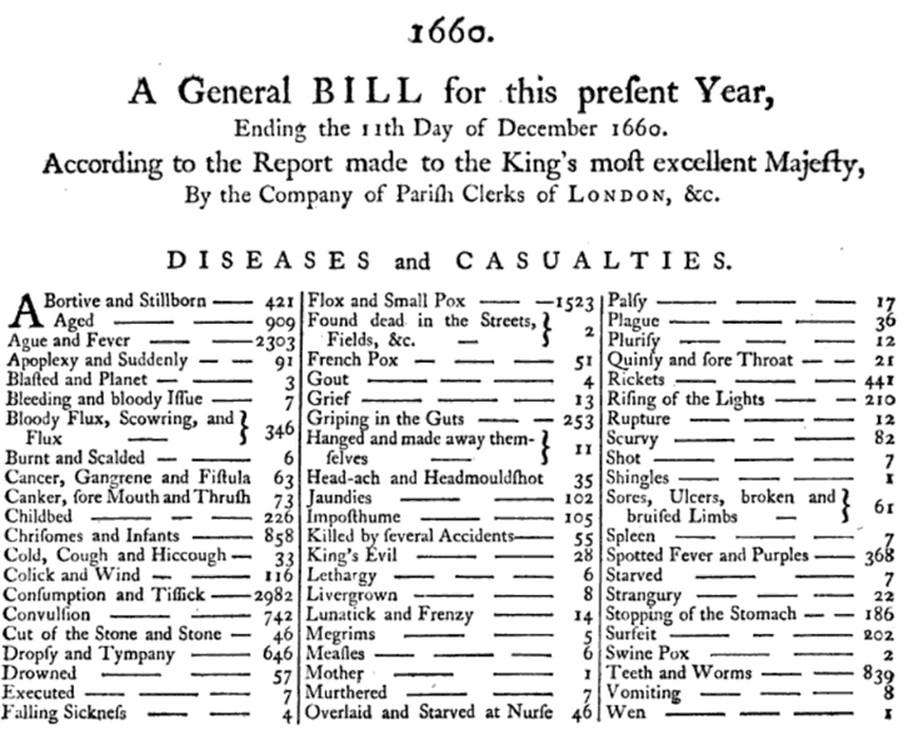
\includegraphics[width=1\linewidth]{images/StandardizedVocabularies/bill} 

}

\caption{1660 London Bill of Mortality, showing the cause of death for deceased inhabitants using a classification system of 62 diseases known at the time.}\label{fig:bill}
\end{figure}

Since then, the classifications have greatly expanded in size and
complexity and spread into other aspects of healthcare, such as
procedures and services, drugs, medical devices, etc. The main
principles have remained the same: they are controlled vocabularies,
terminologies, hierarchies or ontologies that some healthcare
communities agree upon for the purpose of capturing, classifying and
analyzing patient data. Many of these vocabularies are maintained by
public and government agencies with a long-term mandate for doing so.
For example, the World Health Organization (WHO) produces the
International Classification of Disease (ICD) with the recent addition
of its 11th revision (ICD11). Local governments create country-specific
versions, such as ICD10CM (USA), ICD10GM (Germany), etc. Governments
also control the marketing and sale of drugs and maintain national
repositories of such certified drugs. Vocabularies are also used in the
private sector, either as commercial products or for internal use, such
as electronic health record (EHR) systems or for medical insurance claim
reporting.

As a result, each country, region, healthcare system and institution
tends to have their own classifications that would most likely only be
relevant where it is used. This myriad of vocabularies prevents
interoperability of the systems they are used in. Standardization is the
key that enables patient data exchange, unlocks health data analysis on
a global level and allows systematic and standardized research,
including performance characterization and quality assessment. To
address that problem, multinational organizations have sprung up and
started creating broad standards, such as the WHO mentioned above and
the Standard Nomenclature of Medicine (SNOMED) or Logical Observation
Identifiers Names and Codes (LOINC). In the US, the Health IT Standards
Committee (HITAC) recommends the use of SNOMED, LOINC and the drug
vocabulary RxNorm as standards to the National Coordinator for Health IT
(ONC) for use in a common platform for nationwide health information
exchange across diverse entities.

OHDSI developed the OMOP CDM, a global standard for observational
research. As part of the CDM, the OMOP Standardized Vocabularies are
available for two main purposes:

\begin{itemize}
\tightlist
\item
  Common repository of all vocabularies used in the community
\item
  Standardization and mapping for use in research
\end{itemize}

The Standardized Vocabularies are available to the community free of
charge and \textbf{must be used} for OMOP CDM instance \textbf{as its
mandatory reference table}.

\subsection{Building the Standardized
Vocabularies}\label{building-the-standardized-vocabularies}

All vocabularies of the Standardized Vocabularies are consolidated into
the same common format. This relieves the researchers from having to
understand and handle multiple different formats and life-cycle
conventions of the originating vocabularies. All vocabularies are
regularly refreshed and incorporated using the Pallas system.\footnote{\url{https://github.com/OHDSI/Vocabulary-v5.0}}
It is built and run by the OHDSI Vocabulary Team, which is part of the
overall OMOP CDM Workgroup. If you find mistakes please report and help
improve our resource by posting in either the OHDSI Forums\footnote{\url{https://forums.ohdsi.org}}
or CDM Github page.\footnote{\url{https://github.com/OHDSI/CommonDataModel/issues}}
\index{Pallas system}

\subsection{Access to the Standardized
Vocabularies}\label{accessVocabularies}

In order to obtain the Standardized Vocabularies, you do not have to run
Pallas yourself. Instead, you can download the latest version from
ATHENA\footnote{\url{http://athena.ohdsi.org}} and load it into your
local database. ATHENA also allows faceted search of the Vocabularies.
\index{ATHENA} \index{standardized vocabularies!download}
\index{standardized vocabularies!search}

To download a zip file with all Standardized Vocabularies tables select
all the vocabularies you need for your OMOP CDM. Vocabularies with
Standard Concepts (see Section \ref{standardConcepts}) and very common
usage are preselected. Add vocabularies that are used in your source
data. Vocabularies that are proprietary have no select button. Click on
the ``License required'' button to incorporate such a vocabulary into
your list. The Vocabulary Team will contact you and request you
demonstrate your license or help you connect to the right folks to
obtain one.

\subsection{Source of Vocabularies: Adopt Versus
Build}\label{source-of-vocabularies-adopt-versus-build}

OHDSI generally prefers adopting existing vocabularies, rather than
de-novo construction, because (i) many vocabularies have already been
utilized in observational data in the community, and (ii) construction
and maintenance of vocabularies is complex and requires the input of
many stakeholders over long periods of time to mature. For that reason,
dedicated organizations provide vocabularies, which are subject to a
life-cycle of generation, deprecation, merging and splitting (see
Section \ref{conceptLifeCycle}). Currently, OHDSI only produces internal
administrative vocabularies like Type Concepts (e.g.~condition type
concepts). The only exception is RxNorm Extension, a vocabulary covering
drugs that are only used outside the United States (see Section
\ref{rxNormExtension}).

\section{Concepts}\label{concepts}

All clinical events in the OMOP CDM are expressed as concepts, which
represent the semantic notion of each event. They are the fundamental
building blocks of the data records, making almost all tables fully
normalized with few exceptions. Concepts are stored in the CONCEPT table
(see Figure \ref{fig:concept}). \index{concept}

\begin{figure}

{\centering 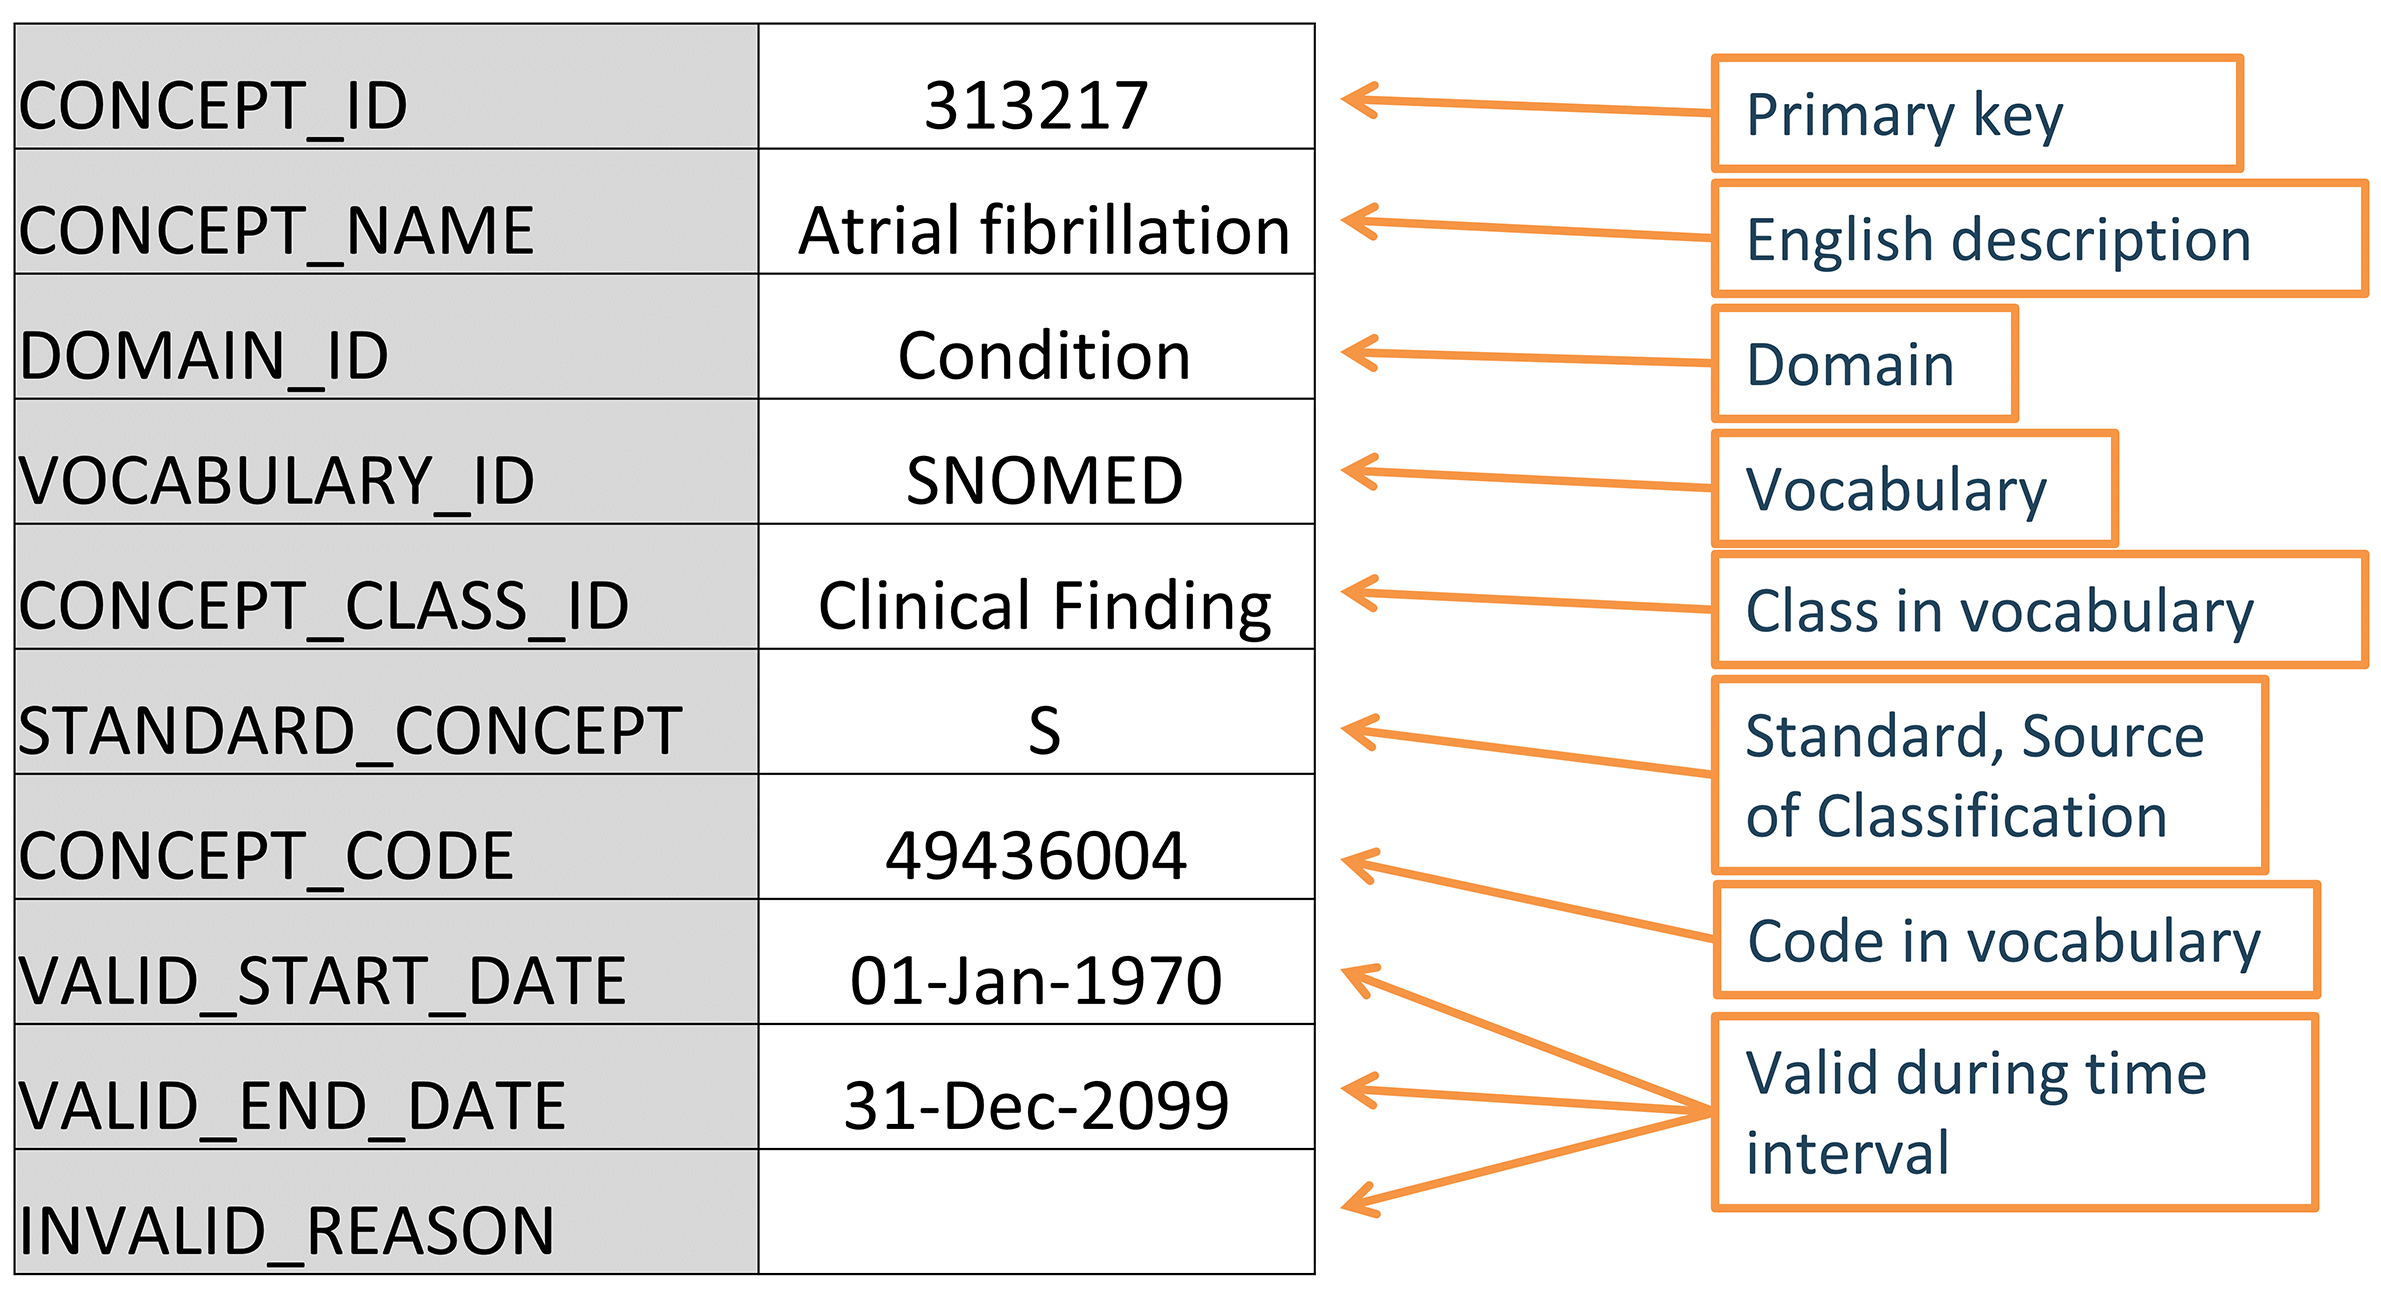
\includegraphics[width=0.9\linewidth]{images/StandardizedVocabularies/concept} 

}

\caption{Standard representation of vocabulary concepts in the OMOP CDM. The example provided is the CONCEPT table record for the SNOMED code for Atrial Fibrillation.}\label{fig:concept}
\end{figure}

This system is meant to be \textbf{comprehensive}, i.e.~there are enough
concepts to cover any event relevant to the patient's healthcare
experience (e.g.~conditions, procedures, exposures to drug, etc.) as
well as some of the administrative information of the healthcare system
(e.g.~visits, care sites, etc.).

\subsection{Concept IDs}\label{concept-ids}

Each concept is assigned a concept ID to be used as a primary key. This
meaningless integer ID, rather than the original code from the
vocabulary, is used to record data in the CDM event tables.
\index{concept!identifier}

\subsection{Concept Names}\label{concept-names}

Each concept has one name. Names are always in English. They are
imported from the source of the vocabulary. If the source vocabulary has
more than one name, the most expressive is selected and the remaining
ones are stored in the CONCEPT\_SYNONYM table under the same CONCEPT\_ID
key. Non-English names are recorded in CONCEPT\_SYNONYM as well, with
the appropriate language concept ID in the LANGUAGE\_CONCEPT\_ID field.
The name is 255 characters long, which means that very long names get
truncated and the full-length version recorded as another synonym, which
can hold up to 1000 characters.

\subsection{Domains}\label{conceptDomains}

Each concept is assigned a domain in the DOMAIN\_ID field, which in
contrast to the numerical CONCEPT\_ID is a short case-sensitive unique
alphanumeric ID for the domain. Examples of such domain identifiers are
``Condition,'' ``Drug,'' ``Procedure,'' ``Visit,'' ``Device,''
``Specimen,'' etc. Ambiguous or pre-coordinated (combination) concepts
can belong to a combination domain, but Standard Concepts (see Section
\ref{standardConcepts}) are always assigned a singular domain. Domains
also direct to which CDM table and field a clinical event or event
attribute is recorded. Domain assignments are an OMOP-specific feature
done during vocabulary ingestion using a heuristic laid out in
\href{https://github.com/ohDSI/vocabulary-v5.0}{Pallas}. Source
vocabularies tend to combine codes of mixed domains, but to a varying
degree (see Figure \ref{fig:domains}). \index{domain!concept}

\begin{figure}

{\centering 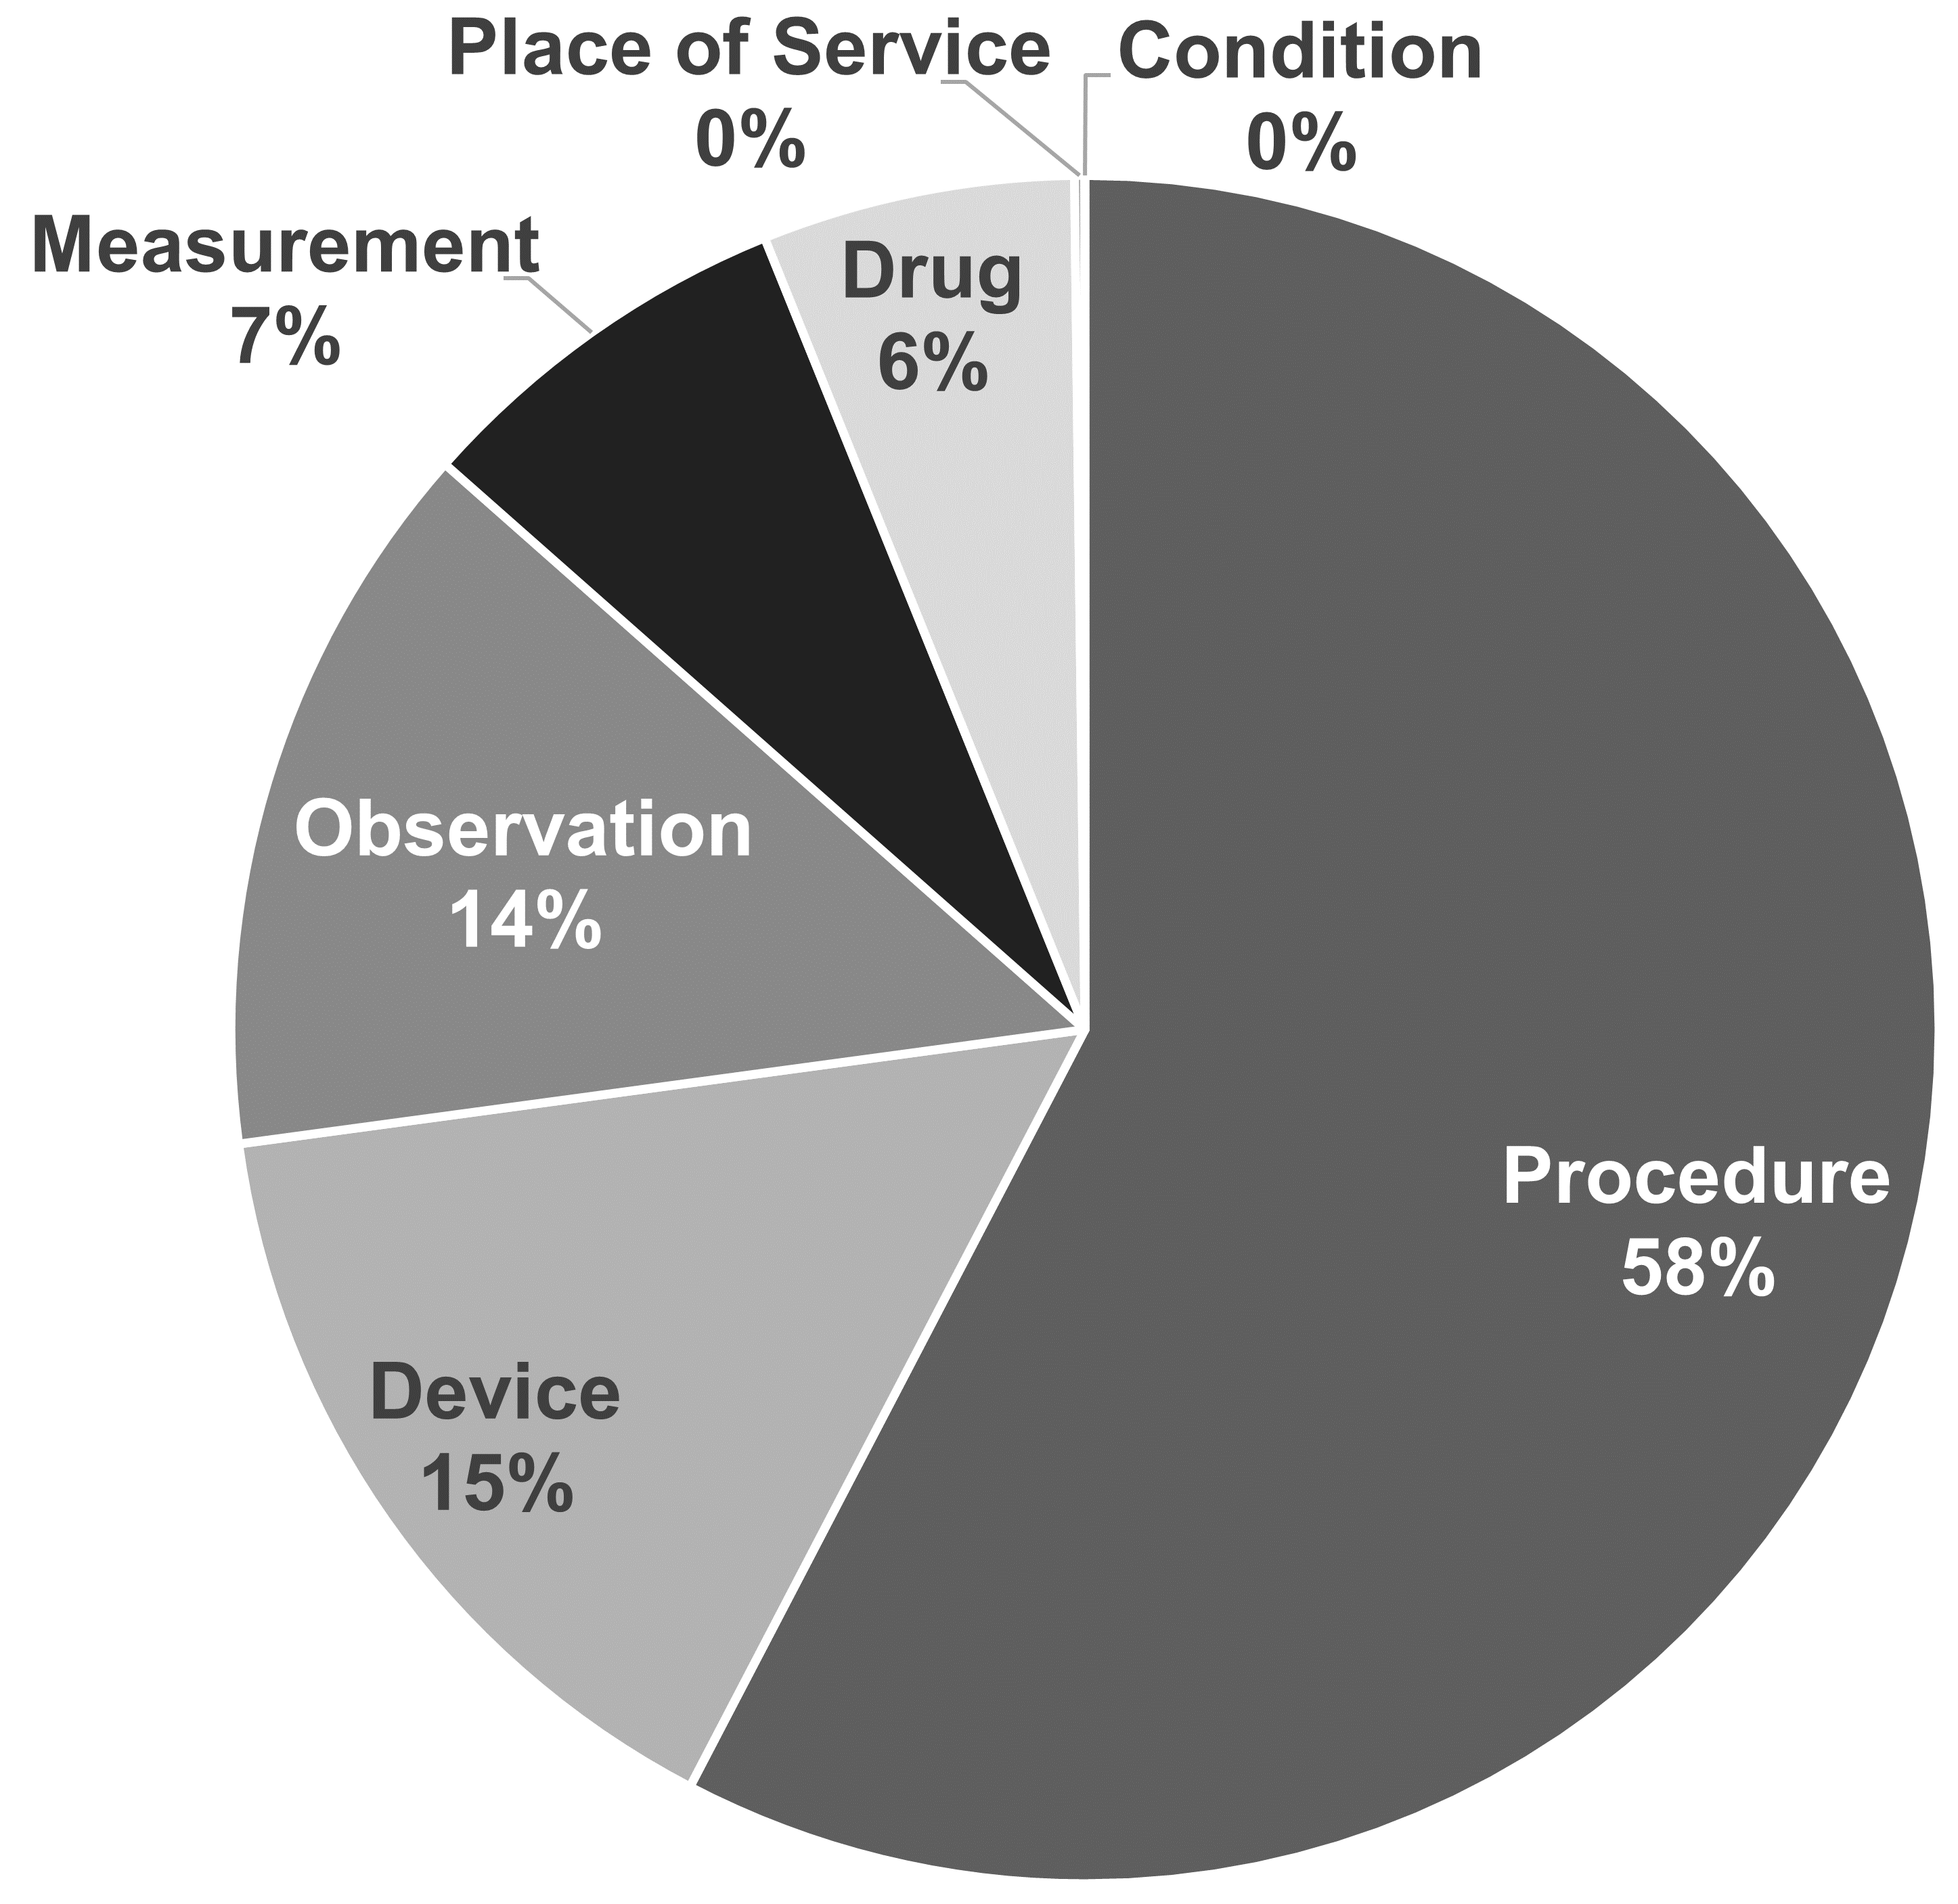
\includegraphics[width=0.7\linewidth]{images/StandardizedVocabularies/domains} 

}

\caption{Domain assignment in procedure vocabularies CPT4 and HCPCS. By intuition, these vocabularies should contain codes and concepts of a single domain, but in reality they are mixed.}\label{fig:domains}
\end{figure}

The domain heuristic follows the definitions of the domains. These
definitions are derived from the table and field definitions in the CDM
(see Chapter \ref{CommonDataModel}). The heuristic is not perfect; there
are grey zones (see Section \ref{specialSituations} ``Special
Situations''). If you find concept domains assigned incorrectly please
report and help improve the process through a
\href{https://forums.ohdsi.org}{Forums} or
\href{https://github.com/OHDSI/CommonDataModel/issues}{CDM issue} post.

\subsection{Vocabularies}\label{vocabularies}

Each vocabulary has a short case-sensitive unique alphanumeric ID, which
generally follows the abbreviated name of the vocabulary, omitting
dashes. For example, ICD-9-CM has the vocabulary ID ``ICD9CM''. There
are 111 vocabularies currently supported by OHDSI, of which 78 are
adopted from external sources, while the rest are OMOP-internal
vocabularies. These vocabularies are typically refreshed at a quarterly
schedule. The source and the version of the vocabularies is defined in
the VOCABULARY reference file. \index{vocabulary}

\subsection{Concept Classes}\label{concept-classes}

Some vocabularies classify their codes or concepts, denoted through
their case-sensitive unique alphanumerical IDs. For example, SNOMED has
33 such concept classes, which SNOMED refers to as ``semantic tags'':
clinical finding, social context, body structure, etc. These are
vertical divisions of the concepts. Others, such as MedDRA or RxNorm,
have concept classes classifying horizontal levels in their stratified
hierarchies. Vocabularies without any concept classes, such as HCPCS,
use the vocabulary ID as the Concept Class ID. \index{concept!class}

\begin{longtable}[]{@{}ll@{}}
\caption{\label{tab:sublassification} Vocabularies with or without
horizontal and vertical sub-classification principles in concept
class.}\tabularnewline
\toprule
\begin{minipage}[b]{0.13\columnwidth}\raggedright\strut
Concept class subdivision principle\strut
\end{minipage} & \begin{minipage}[b]{0.47\columnwidth}\raggedright\strut
Vocabulary\strut
\end{minipage}\tabularnewline
\midrule
\endfirsthead
\toprule
\begin{minipage}[b]{0.13\columnwidth}\raggedright\strut
Concept class subdivision principle\strut
\end{minipage} & \begin{minipage}[b]{0.47\columnwidth}\raggedright\strut
Vocabulary\strut
\end{minipage}\tabularnewline
\midrule
\endhead
\begin{minipage}[t]{0.13\columnwidth}\raggedright\strut
Horizontal\strut
\end{minipage} & \begin{minipage}[t]{0.47\columnwidth}\raggedright\strut
all drug vocabularies, ATC, CDТ, Episode, HCPCS, HemOnc, ICDs, MedDRA,
OSM, Census\strut
\end{minipage}\tabularnewline
\begin{minipage}[t]{0.13\columnwidth}\raggedright\strut
Vertical\strut
\end{minipage} & \begin{minipage}[t]{0.47\columnwidth}\raggedright\strut
CIEL, HES Specialty, ICDO3, MeSH, NAACCR, NDFRT, OPCS4, PCORNET, Plan,
PPI, Provider, SNOMED, SPL, UCUM\strut
\end{minipage}\tabularnewline
\begin{minipage}[t]{0.13\columnwidth}\raggedright\strut
Mixed\strut
\end{minipage} & \begin{minipage}[t]{0.47\columnwidth}\raggedright\strut
CPT4, ISBT, LOINC\strut
\end{minipage}\tabularnewline
\begin{minipage}[t]{0.13\columnwidth}\raggedright\strut
None\strut
\end{minipage} & \begin{minipage}[t]{0.47\columnwidth}\raggedright\strut
APC, all Type Concepts, Ethnicity, OXMIS, Race, Revenue Code, Sponsor,
Supplier, UB04s, Visit\strut
\end{minipage}\tabularnewline
\bottomrule
\end{longtable}

Horizontal concept classes allow you to determine a specific
hierarchical level. For example, in the drug vocabulary RxNorm the
concept class ``Ingredient'' defines the top level of the hierarchy. In
the vertical model, members of a concept class can be of any
hierarchical level from the top to the very bottom.

\subsection{Standard Concepts}\label{standardConcepts}

One concept representing the meaning of each clinical event is
designated the Standard. For example, MESH code D001281, CIEL code
148203, SNOMED code 49436004, ICD9CM code 427.31 and Read code G573000
all define ``Atrial fibrillation'' in the condition domain, but only the
SNOMED concept is Standard and represents the condition in the data. The
others are designated non-standard or source concepts and mapped to the
Standard ones. Standard Concepts are indicated through an ``S'' in the
STANDARD\_CONCEPT field. And only these Standard Concepts are used to
record data in the CDM fields ending in ``\_CONCEPT\_ID``.
\index{standard concept}

\subsection{Non-Standard Concepts}\label{non-standard-concepts}

Non-standard concepts are not used to represent the clinical events, but
they are still part of the Standardized Vocabularies, and are often
found in the source data. For that reason, they are also called ``source
concepts''. The conversion of source concepts to Standard Concepts is a
process called ``mapping'' (see Section \ref{conceptMapping}).
Non-standard concepts have no value (NULL) In the STANDARD\_CONCEPT
field.

\subsection{Classification Concepts}\label{classification-concepts}

These concepts are not Standard, and hence cannot be used to represent
the data. But they are participating in the hierarchy with the Standard
Concepts, and can therefore be used to perform hierarchical queries. For
example, querying for all descendants of MedDRA code 10037908 (not
visible for users who have not obtained a MedDRA license, see Section
\ref{accessVocabularies} for access restrictions) will retrieve the
Standard SNOMED concept for Atrial Fibrillation (see Section
\ref{conceptAncestor} for hierarchical queries using the
CONCEPT\_ANCESTOR table) - see Figure \ref{fig:hierarchy}.
\index{classification concept}

\begin{figure}

{\centering 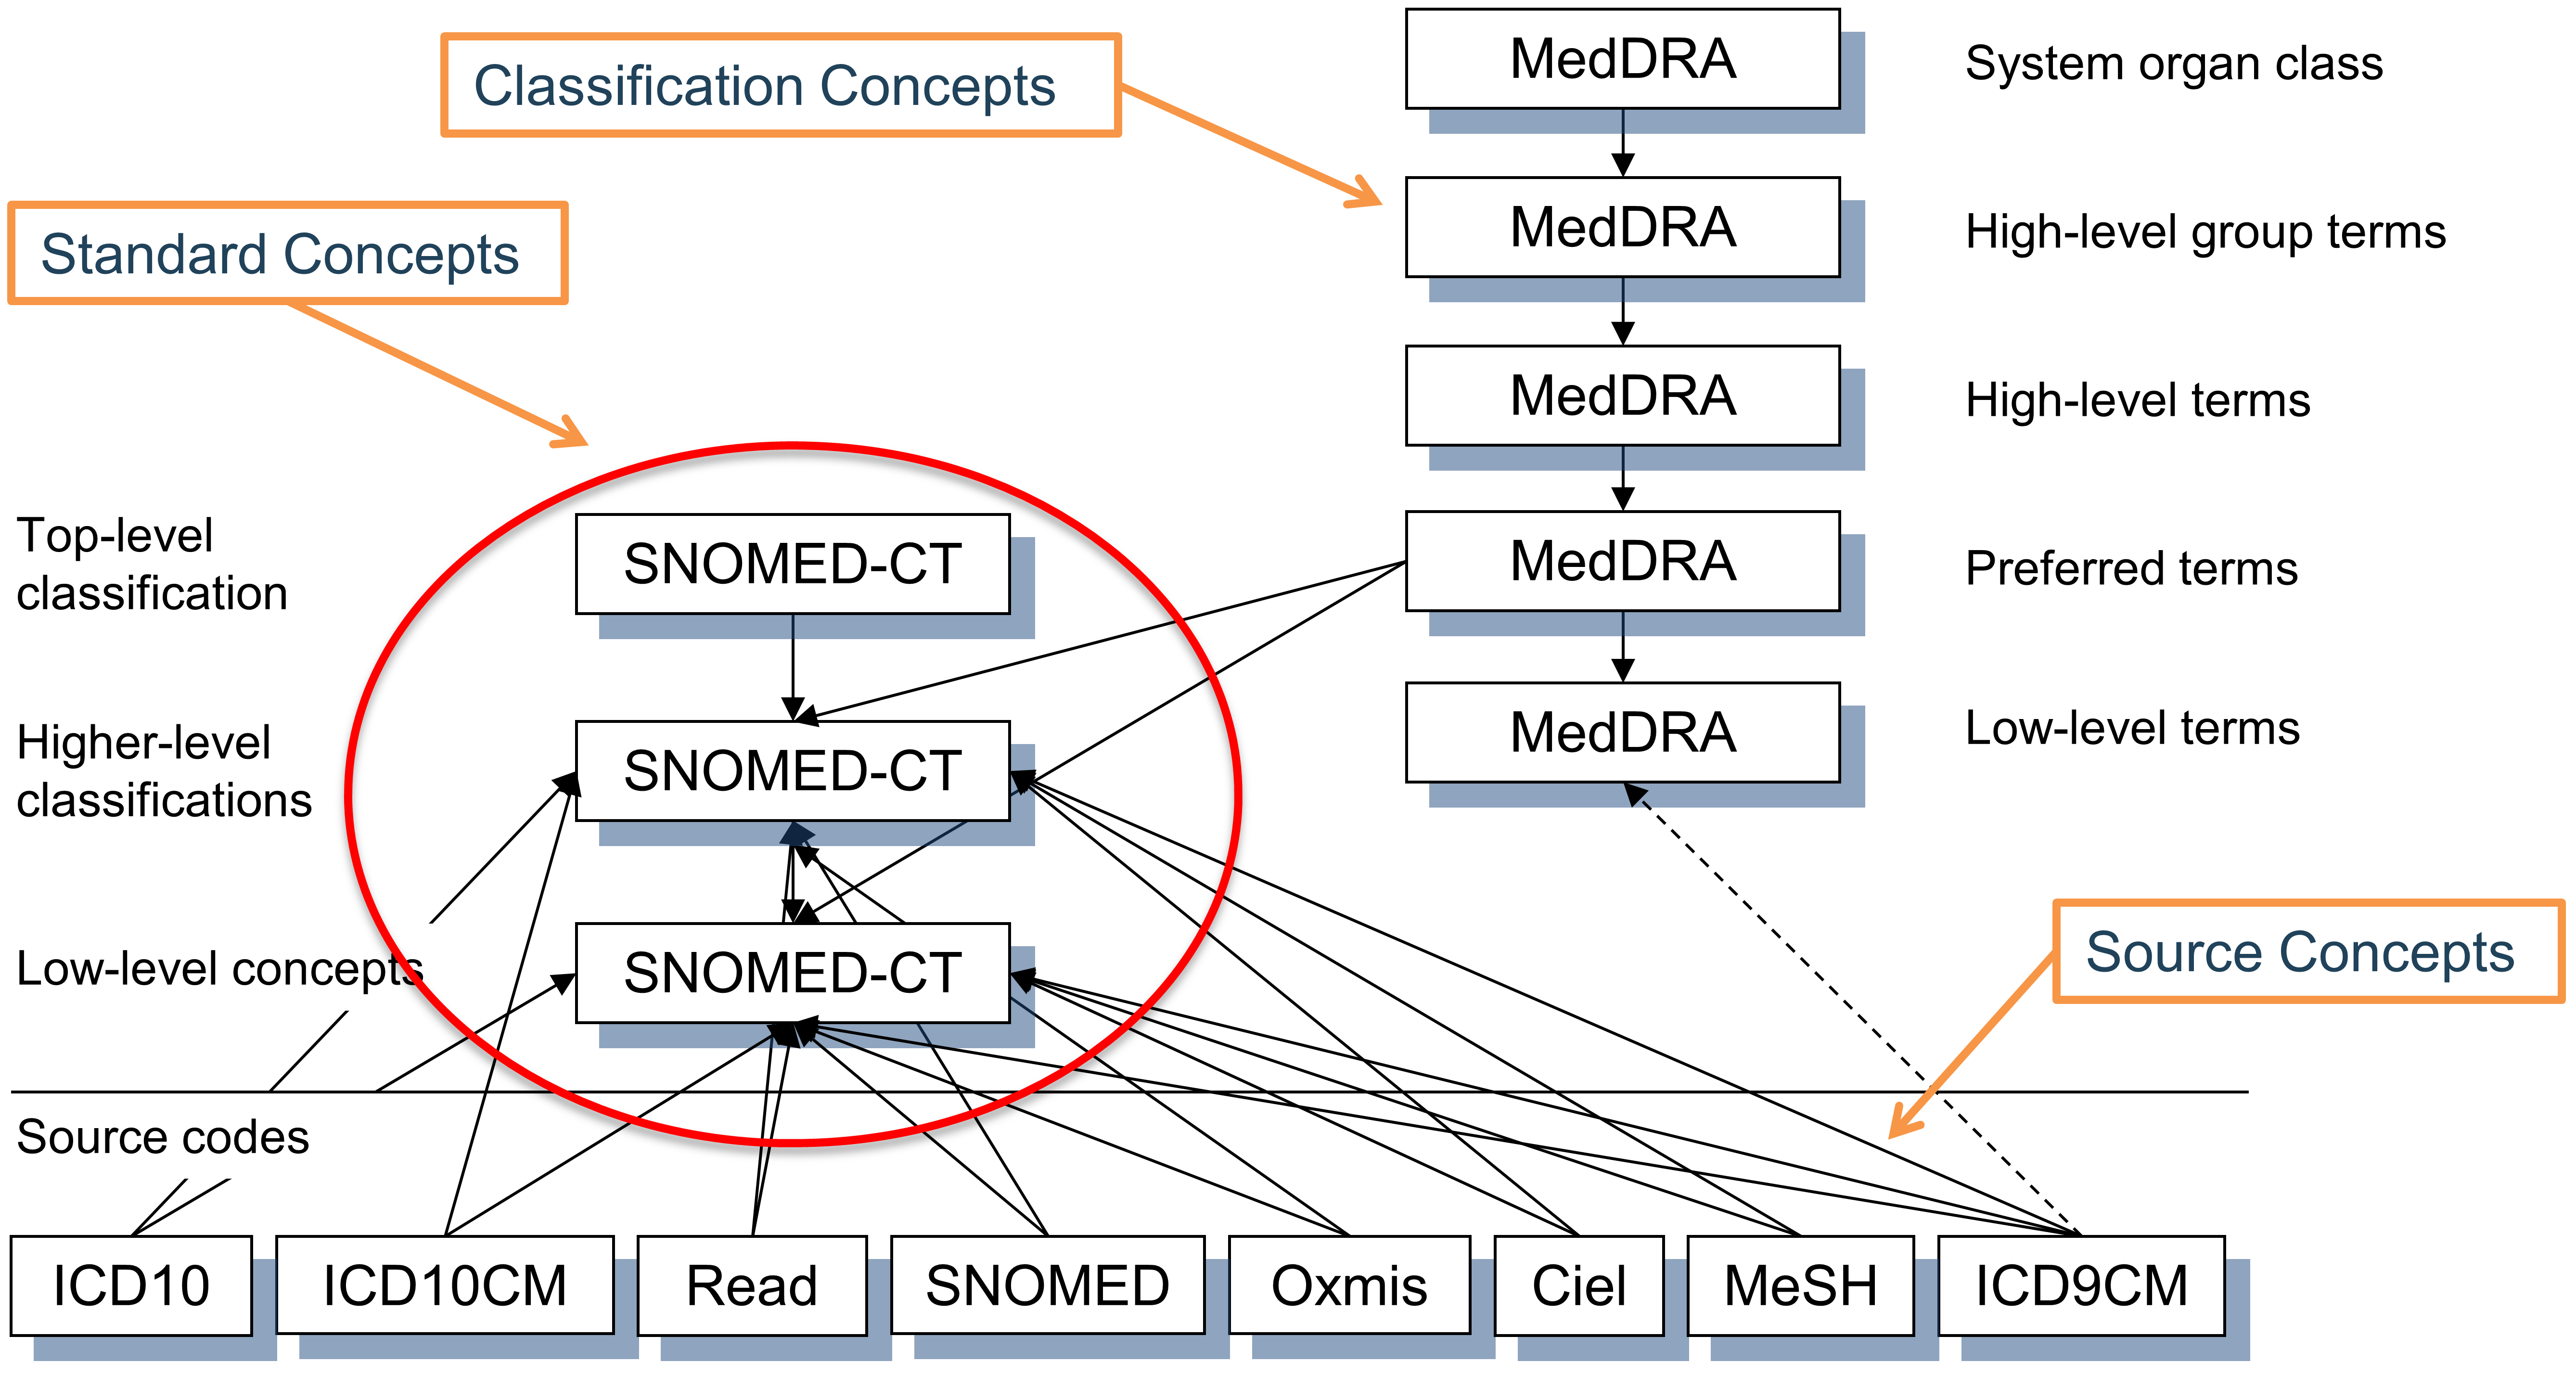
\includegraphics[width=1\linewidth]{images/StandardizedVocabularies/hierarchy} 

}

\caption{Standard, non-standard source and classification concepts and their hierarchical relationships in the condition domain. SNOMED is used for most standard condition concepts (with some oncology-related concepts derived from ICDO3), MedDRA concepts are used for hierarchical classification concepts, and all other vocabularies contain non-standard or source concepts, which do not participate in the hierarchy.}\label{fig:hierarchy}
\end{figure}

The choice of concept designation as Standard, non-standard and
classification is typically done for each domain separately at the
vocabulary level. This is based on the quality of the concepts, the
built-in hierarchy and the declared purpose of the vocabulary. Also, not
all concepts of a vocabulary are used as Standard Concepts. The
designation is separate for each domain, each concept has to be active
(see Section \ref{conceptLifeCycle}) and there might be an order of
precedence if more than one concept from different vocabularies compete
for the same meaning. In other words, there is no such a thing as a
``standard vocabulary.'' See Table \ref{tab:vocabList} for examples.

\begin{longtable}[]{@{}llll@{}}
\caption{\label{tab:vocabList} List of vocabularies to utilize for
Standard/non-standard/classification concept
assignments.}\tabularnewline
\toprule
\begin{minipage}[b]{0.12\columnwidth}\raggedright\strut
Domain\strut
\end{minipage} & \begin{minipage}[b]{0.21\columnwidth}\raggedright\strut
for Standard Concepts\strut
\end{minipage} & \begin{minipage}[b]{0.21\columnwidth}\raggedright\strut
for source concepts\strut
\end{minipage} & \begin{minipage}[b]{0.18\columnwidth}\raggedright\strut
for classification concepts\strut
\end{minipage}\tabularnewline
\midrule
\endfirsthead
\toprule
\begin{minipage}[b]{0.12\columnwidth}\raggedright\strut
Domain\strut
\end{minipage} & \begin{minipage}[b]{0.21\columnwidth}\raggedright\strut
for Standard Concepts\strut
\end{minipage} & \begin{minipage}[b]{0.21\columnwidth}\raggedright\strut
for source concepts\strut
\end{minipage} & \begin{minipage}[b]{0.18\columnwidth}\raggedright\strut
for classification concepts\strut
\end{minipage}\tabularnewline
\midrule
\endhead
\begin{minipage}[t]{0.12\columnwidth}\raggedright\strut
Condition\strut
\end{minipage} & \begin{minipage}[t]{0.21\columnwidth}\raggedright\strut
SNOMED, ICDO3\strut
\end{minipage} & \begin{minipage}[t]{0.21\columnwidth}\raggedright\strut
SNOMED Veterinary\strut
\end{minipage} & \begin{minipage}[t]{0.18\columnwidth}\raggedright\strut
MedDRA\strut
\end{minipage}\tabularnewline
\begin{minipage}[t]{0.12\columnwidth}\raggedright\strut
Procedure\strut
\end{minipage} & \begin{minipage}[t]{0.21\columnwidth}\raggedright\strut
SNOMED, CPT4, HCPCS, ICD10PCS, ICD9Proc, OPCS4\strut
\end{minipage} & \begin{minipage}[t]{0.21\columnwidth}\raggedright\strut
SNOMED Veterinary, HemOnc, NAACCR\strut
\end{minipage} & \begin{minipage}[t]{0.18\columnwidth}\raggedright\strut
None at this point\strut
\end{minipage}\tabularnewline
\begin{minipage}[t]{0.12\columnwidth}\raggedright\strut
Measurement\strut
\end{minipage} & \begin{minipage}[t]{0.21\columnwidth}\raggedright\strut
SNOMED, LOINC\strut
\end{minipage} & \begin{minipage}[t]{0.21\columnwidth}\raggedright\strut
SNOMED Veterinary, NAACCR, CPT4, HCPCS, OPCS4, PPI\strut
\end{minipage} & \begin{minipage}[t]{0.18\columnwidth}\raggedright\strut
None at this point\strut
\end{minipage}\tabularnewline
\begin{minipage}[t]{0.12\columnwidth}\raggedright\strut
Drug\strut
\end{minipage} & \begin{minipage}[t]{0.21\columnwidth}\raggedright\strut
RxNorm, RxNorm Extension, CVX\strut
\end{minipage} & \begin{minipage}[t]{0.21\columnwidth}\raggedright\strut
HCPCS, CPT4, HemOnc, NAAACCR\strut
\end{minipage} & \begin{minipage}[t]{0.18\columnwidth}\raggedright\strut
ATC\strut
\end{minipage}\tabularnewline
\begin{minipage}[t]{0.12\columnwidth}\raggedright\strut
Device\strut
\end{minipage} & \begin{minipage}[t]{0.21\columnwidth}\raggedright\strut
SNOMED\strut
\end{minipage} & \begin{minipage}[t]{0.21\columnwidth}\raggedright\strut
Others, currently not normalized\strut
\end{minipage} & \begin{minipage}[t]{0.18\columnwidth}\raggedright\strut
None at this point\strut
\end{minipage}\tabularnewline
\begin{minipage}[t]{0.12\columnwidth}\raggedright\strut
Observation\strut
\end{minipage} & \begin{minipage}[t]{0.21\columnwidth}\raggedright\strut
SNOMED\strut
\end{minipage} & \begin{minipage}[t]{0.21\columnwidth}\raggedright\strut
Others\strut
\end{minipage} & \begin{minipage}[t]{0.18\columnwidth}\raggedright\strut
None at this point\strut
\end{minipage}\tabularnewline
\begin{minipage}[t]{0.12\columnwidth}\raggedright\strut
Visit\strut
\end{minipage} & \begin{minipage}[t]{0.21\columnwidth}\raggedright\strut
CMS Place of Service, ABMT, NUCC\strut
\end{minipage} & \begin{minipage}[t]{0.21\columnwidth}\raggedright\strut
SNOMED, HCPCS, CPT4, UB04\strut
\end{minipage} & \begin{minipage}[t]{0.18\columnwidth}\raggedright\strut
None at this point\strut
\end{minipage}\tabularnewline
\bottomrule
\end{longtable}

\subsection{Concept Codes}\label{concept-codes}

Concept codes are the identifiers used in the source vocabularies. For
example, ICD9CM or NDC codes are stored in this field, while the OMOP
tables use the concept ID as a foreign key into the CONCEPT table. The
reason is that the name space overlaps across vocabularies, i.e.~the
same code can exist in different vocabularies with completely different
meanings (see Table \ref{tab:code1001}) \index{concept!code}

\begin{longtable}[]{@{}llllll@{}}
\caption{\label{tab:code1001} Concepts with identical concept code 1001, but
different vocabularies, domains and concept classes.}\tabularnewline
\toprule
\begin{minipage}[b]{0.13\columnwidth}\raggedright\strut
Concept ID\strut
\end{minipage} & \begin{minipage}[b]{0.07\columnwidth}\raggedright\strut
Concept Code\strut
\end{minipage} & \begin{minipage}[b]{0.16\columnwidth}\raggedright\strut
Concept Name\strut
\end{minipage} & \begin{minipage}[b]{0.14\columnwidth}\raggedright\strut
Domain ID\strut
\end{minipage} & \begin{minipage}[b]{0.14\columnwidth}\raggedright\strut
Vocabulary ID\strut
\end{minipage} & \begin{minipage}[b]{0.14\columnwidth}\raggedright\strut
Concept Class\strut
\end{minipage}\tabularnewline
\midrule
\endfirsthead
\toprule
\begin{minipage}[b]{0.13\columnwidth}\raggedright\strut
Concept ID\strut
\end{minipage} & \begin{minipage}[b]{0.07\columnwidth}\raggedright\strut
Concept Code\strut
\end{minipage} & \begin{minipage}[b]{0.16\columnwidth}\raggedright\strut
Concept Name\strut
\end{minipage} & \begin{minipage}[b]{0.14\columnwidth}\raggedright\strut
Domain ID\strut
\end{minipage} & \begin{minipage}[b]{0.14\columnwidth}\raggedright\strut
Vocabulary ID\strut
\end{minipage} & \begin{minipage}[b]{0.14\columnwidth}\raggedright\strut
Concept Class\strut
\end{minipage}\tabularnewline
\midrule
\endhead
\begin{minipage}[t]{0.13\columnwidth}\raggedright\strut
35803438\strut
\end{minipage} & \begin{minipage}[t]{0.07\columnwidth}\raggedright\strut
1001\strut
\end{minipage} & \begin{minipage}[t]{0.16\columnwidth}\raggedright\strut
Granulocyte colony-stimulating factors\strut
\end{minipage} & \begin{minipage}[t]{0.14\columnwidth}\raggedright\strut
Drug\strut
\end{minipage} & \begin{minipage}[t]{0.14\columnwidth}\raggedright\strut
HemOnc\strut
\end{minipage} & \begin{minipage}[t]{0.14\columnwidth}\raggedright\strut
Component Class\strut
\end{minipage}\tabularnewline
\begin{minipage}[t]{0.13\columnwidth}\raggedright\strut
35942070\strut
\end{minipage} & \begin{minipage}[t]{0.07\columnwidth}\raggedright\strut
1001\strut
\end{minipage} & \begin{minipage}[t]{0.16\columnwidth}\raggedright\strut
AJCC TNM Clin T\strut
\end{minipage} & \begin{minipage}[t]{0.14\columnwidth}\raggedright\strut
Measurement\strut
\end{minipage} & \begin{minipage}[t]{0.14\columnwidth}\raggedright\strut
NAACCR\strut
\end{minipage} & \begin{minipage}[t]{0.14\columnwidth}\raggedright\strut
NAACCR Variable\strut
\end{minipage}\tabularnewline
\begin{minipage}[t]{0.13\columnwidth}\raggedright\strut
1036059\strut
\end{minipage} & \begin{minipage}[t]{0.07\columnwidth}\raggedright\strut
1001\strut
\end{minipage} & \begin{minipage}[t]{0.16\columnwidth}\raggedright\strut
Antipyrine\strut
\end{minipage} & \begin{minipage}[t]{0.14\columnwidth}\raggedright\strut
Drug\strut
\end{minipage} & \begin{minipage}[t]{0.14\columnwidth}\raggedright\strut
RxNorm\strut
\end{minipage} & \begin{minipage}[t]{0.14\columnwidth}\raggedright\strut
Ingredient\strut
\end{minipage}\tabularnewline
\begin{minipage}[t]{0.13\columnwidth}\raggedright\strut
38003544\strut
\end{minipage} & \begin{minipage}[t]{0.07\columnwidth}\raggedright\strut
1001\strut
\end{minipage} & \begin{minipage}[t]{0.16\columnwidth}\raggedright\strut
Residential Treatment - Psychiatric\strut
\end{minipage} & \begin{minipage}[t]{0.14\columnwidth}\raggedright\strut
Revenue Code\strut
\end{minipage} & \begin{minipage}[t]{0.14\columnwidth}\raggedright\strut
Revenue Code\strut
\end{minipage} & \begin{minipage}[t]{0.14\columnwidth}\raggedright\strut
Revenue Code\strut
\end{minipage}\tabularnewline
\begin{minipage}[t]{0.13\columnwidth}\raggedright\strut
43228317\strut
\end{minipage} & \begin{minipage}[t]{0.07\columnwidth}\raggedright\strut
1001\strut
\end{minipage} & \begin{minipage}[t]{0.16\columnwidth}\raggedright\strut
Aceprometazine maleate\strut
\end{minipage} & \begin{minipage}[t]{0.14\columnwidth}\raggedright\strut
Drug\strut
\end{minipage} & \begin{minipage}[t]{0.14\columnwidth}\raggedright\strut
BDPM\strut
\end{minipage} & \begin{minipage}[t]{0.14\columnwidth}\raggedright\strut
Ingredient\strut
\end{minipage}\tabularnewline
\begin{minipage}[t]{0.13\columnwidth}\raggedright\strut
45417187\strut
\end{minipage} & \begin{minipage}[t]{0.07\columnwidth}\raggedright\strut
1001\strut
\end{minipage} & \begin{minipage}[t]{0.16\columnwidth}\raggedright\strut
Brompheniramine Maleate, 10 mg/mL injectable solution\strut
\end{minipage} & \begin{minipage}[t]{0.14\columnwidth}\raggedright\strut
Drug\strut
\end{minipage} & \begin{minipage}[t]{0.14\columnwidth}\raggedright\strut
Multum\strut
\end{minipage} & \begin{minipage}[t]{0.14\columnwidth}\raggedright\strut
Multum\strut
\end{minipage}\tabularnewline
\begin{minipage}[t]{0.13\columnwidth}\raggedright\strut
45912144\strut
\end{minipage} & \begin{minipage}[t]{0.07\columnwidth}\raggedright\strut
1001\strut
\end{minipage} & \begin{minipage}[t]{0.16\columnwidth}\raggedright\strut
Serum\strut
\end{minipage} & \begin{minipage}[t]{0.14\columnwidth}\raggedright\strut
Specimen\strut
\end{minipage} & \begin{minipage}[t]{0.14\columnwidth}\raggedright\strut
CIEL\strut
\end{minipage} & \begin{minipage}[t]{0.14\columnwidth}\raggedright\strut
Specimen\strut
\end{minipage}\tabularnewline
\bottomrule
\end{longtable}

\subsection{Life-Cycle}\label{conceptLifeCycle}

Vocabularies are rarely permanent corpora with a fixed set of codes.
Instead, codes and concepts are added and get deprecated. The OMOP CDM
is a model to support longitudinal patient data, which means it needs to
support concepts that were used in the past and might no longer be
active, as well as supporting new concepts and placing them into
context. There are three fields in the CONCEPT table that describe the
possible life-cycle statuses: VALID\_START\_DATE, VALID\_END\_DATE, and
INVALID\_REASON. Their values differ depending on the concept life-cycle
status:

\begin{itemize}
\tightlist
\item
  \textbf{Active or new concept}

  \begin{itemize}
  \tightlist
  \item
    Description: Concept in use.
  \item
    VALID\_START\_DATE: Day of instantiation of concept, if that is not
    known day of incorporation of concept in Vocabularies, if that is
    not known 1970-1-1.
  \item
    VALID\_END\_DATE: Set to 2099-12-31 as a convention to indicate
    ``Might become invalid in an undefined future, but active right
    now''.
  \item
    INVALID\_REASON: NULL
  \end{itemize}
\item
  \textbf{Deprecated Concept with no successor}

  \begin{itemize}
  \tightlist
  \item
    Description: Concept inactive and cannot be used as Standard (see
    Section \ref{standardConcepts}).
  \item
    VALID\_START\_DATE: Day of instantiation of concept, if that is not
    known day of incorporation of concept in Vocabularies, if that is
    not known 1970-1-1.
  \item
    VALID\_END\_DATE: Day in the past indicating deprecation, or if that
    is not known day of vocabulary refresh where concept in vocabulary
    went missing or set to inactive.
  \item
    INVALID\_REASON: ``D''
  \end{itemize}
\item
  \textbf{Upgraded Concept with successor}

  \begin{itemize}
  \tightlist
  \item
    Description: Concept inactive, but has defined successor. These are
    typically concepts which went through de-duplication.
  \item
    VALID\_START\_DATE: Day of instantiation of concept, if that is not
    known day of incorporation of concept in Vocabularies, if that is
    not known 1970-1-1.
  \item
    VALID\_END\_DATE: Day in the past indicating an upgrade, or if that
    is not known day of vocabulary refresh where the upgrade was
    included.
  \item
    INVALID\_REASON: ``U''
  \end{itemize}
\item
  \textbf{Reused code for another new concept}

  \begin{itemize}
  \tightlist
  \item
    Description: The vocabulary reused the concept code of this
    deprecated concept for a new concept.
  \item
    VALID\_START\_DATE: Day of instantiation of concept, if that is not
    known day of incorporation of concept in Vocabularies, if that is
    not known 1970-1-1.
  \item
    VALID\_END\_DATE: Day in the past indicating deprecation, or if that
    is not known day of vocabulary refresh where concept in vocabulary
    went missing or set to inactive.
  \item
    INVALID\_REASON: ``R''
  \end{itemize}
\end{itemize}

In general, concept codes are not reused. But there are a few
vocabularies that deviate from this rule, in particular HCPCS, NDC and
DRG. For those, the same concept code appears in more than one concept
of the same vocabulary. Their CONCEPT\_ID value stays unique. These
reused concept codes are marked with an ``R'' in the INVALID\_REASON
field, and the VALID\_START\_DATE to VALID\_END\_DATE period should be
used to distinguish concepts with the same concept codes.

\section{Relationships}\label{relationships}

Any two concepts can have a defined relationship, regardless of whether
the two concepts belong to the same domain or vocabulary. The nature of
the relationships is indicated in its short case-sensitive unique
alphanumeric ID in the RELATIONSHIP\_ID field of the
CONCEPT\_RELATIONSHIP table. Relationships are symmetrical, i.e.~for
each relationship an equivalent relationship exists, where the content
of the fields CONCEPT\_ID\_1 and CONCEPT\_ID\_2 are swapped, and the
RELATIONHSIP\_ID is changed to its opposite. For example, the ``Maps
to'' relationship has an opposite relationship ``Mapped from.''
\index{concept!relationship}

CONCEPT\_RELATIONSHIP table records also have life-cycle fields
RELATIONSHIP\_START\_DATE, RELATIONSHIP\_END\_DATE and INVALID\_REASON.
However, only active records with INVALID\_REASON = NULL are available
through ATHENA. Inactive relationships are kept in the Pallas system for
internal processing only. The RELATIONSHIP table serves as the reference
with the full list of relationship IDs and their reverse counterparts.

\subsection{Mapping Relationships}\label{conceptMapping}

These relationships provide translations from non-standard to Standard
concepts, supported by two relationship ID pairs (see Table
\ref{tab:mappingRelationships}). \index{concept!mapping}

\begin{longtable}[]{@{}ll@{}}
\caption{\label{tab:mappingRelationships} Type of mapping
relationships.}\tabularnewline
\toprule
\begin{minipage}[b]{0.20\columnwidth}\raggedright\strut
Relationship ID pair\strut
\end{minipage} & \begin{minipage}[b]{0.71\columnwidth}\raggedright\strut
Purpose\strut
\end{minipage}\tabularnewline
\midrule
\endfirsthead
\toprule
\begin{minipage}[b]{0.20\columnwidth}\raggedright\strut
Relationship ID pair\strut
\end{minipage} & \begin{minipage}[b]{0.71\columnwidth}\raggedright\strut
Purpose\strut
\end{minipage}\tabularnewline
\midrule
\endhead
\begin{minipage}[t]{0.20\columnwidth}\raggedright\strut
``Maps to'' and ``Mapped from''\strut
\end{minipage} & \begin{minipage}[t]{0.71\columnwidth}\raggedright\strut
Mapping to Standard Concepts. Standard Concepts are mapped to
themselves, non-standard concepts to Standard Concepts. Most
non-standard and all Standard Concepts have this relationship to a
Standard Concept. The former are stored in *\_SOURCE\_CONCEPT\_ID, and
the latter in the *\_CONCEPT\_ID fields. Classification concepts are not
mapped.\strut
\end{minipage}\tabularnewline
\begin{minipage}[t]{0.20\columnwidth}\raggedright\strut
``Maps to value'' and ``Value mapped from''\strut
\end{minipage} & \begin{minipage}[t]{0.71\columnwidth}\raggedright\strut
Mapping to a concept that represents a Value to be placed into the
VALUE\_AS\_CONCEPT\_ID fields of the MEASUREMENT and OBSERVATION
tables.\strut
\end{minipage}\tabularnewline
\bottomrule
\end{longtable}

The purpose of these mapping relationships is to allow a crosswalk
between equivalent concepts to harmonize how clinical events are
represented in the OMOP CDM. This is a main achievement of the
Standardized Vocabularies.

``Equivalent concepts'' means it carries the same meaning, and,
importantly, the hierarchical descendants cover the same semantic space.
If an equivalent concept is not available and the concept is not
Standard, it is still mapped, but to a slightly broader concept
(so-called ``up-hill mappings''). For example, ICD10CM W61.51 ``Bitten
by goose'' has no equivalent in the SNOMED vocabulary, which is
generally used for standard condition concepts. Instead, it is mapped to
SNOMED 217716004 ``Peck by bird,'' losing the context of the bird being
a goose. Up-hill mappings are only used if the loss of information is
considered irrelevant to standard research use cases.

Some mappings connect a source concept to more than one Standard
Concept. For example, ICD9CM 070.43 ``Hepatitis E with hepatic coma'' is
mapped to both SNOMED 235867002 ``Acute hepatitis E'' as well as SNOMED
72836002 ``Hepatic Coma.'' The reason for this is that the original
source concept is a pre-coordinated combination of two conditions,
hepatitis and coma. SNOMED does not have that combination, which results
in two records written for the ICD9CM record, one with each mapped
Standard Concept.

Relationships ``Maps to value'' have the purpose of splitting of a value
for OMOP CDM tables following an entity-attribute-value (EAV) model.
This is typically the case in the following situations:

\begin{itemize}
\tightlist
\item
  Measurements consisting of a test and a result value
\item
  Personal or family disease history
\item
  Allergy to substance
\item
  Need for immunization
\end{itemize}

In these situations, the source concept is a combination of the
attribute (test or history) and the value (test result or disease). The
``Maps to'' relationship maps this source to the attribute concept, and
the ``Maps to value'' to the value concept. See Figure
\ref{fig:conceptValue} for an example.

\begin{figure}

{\centering 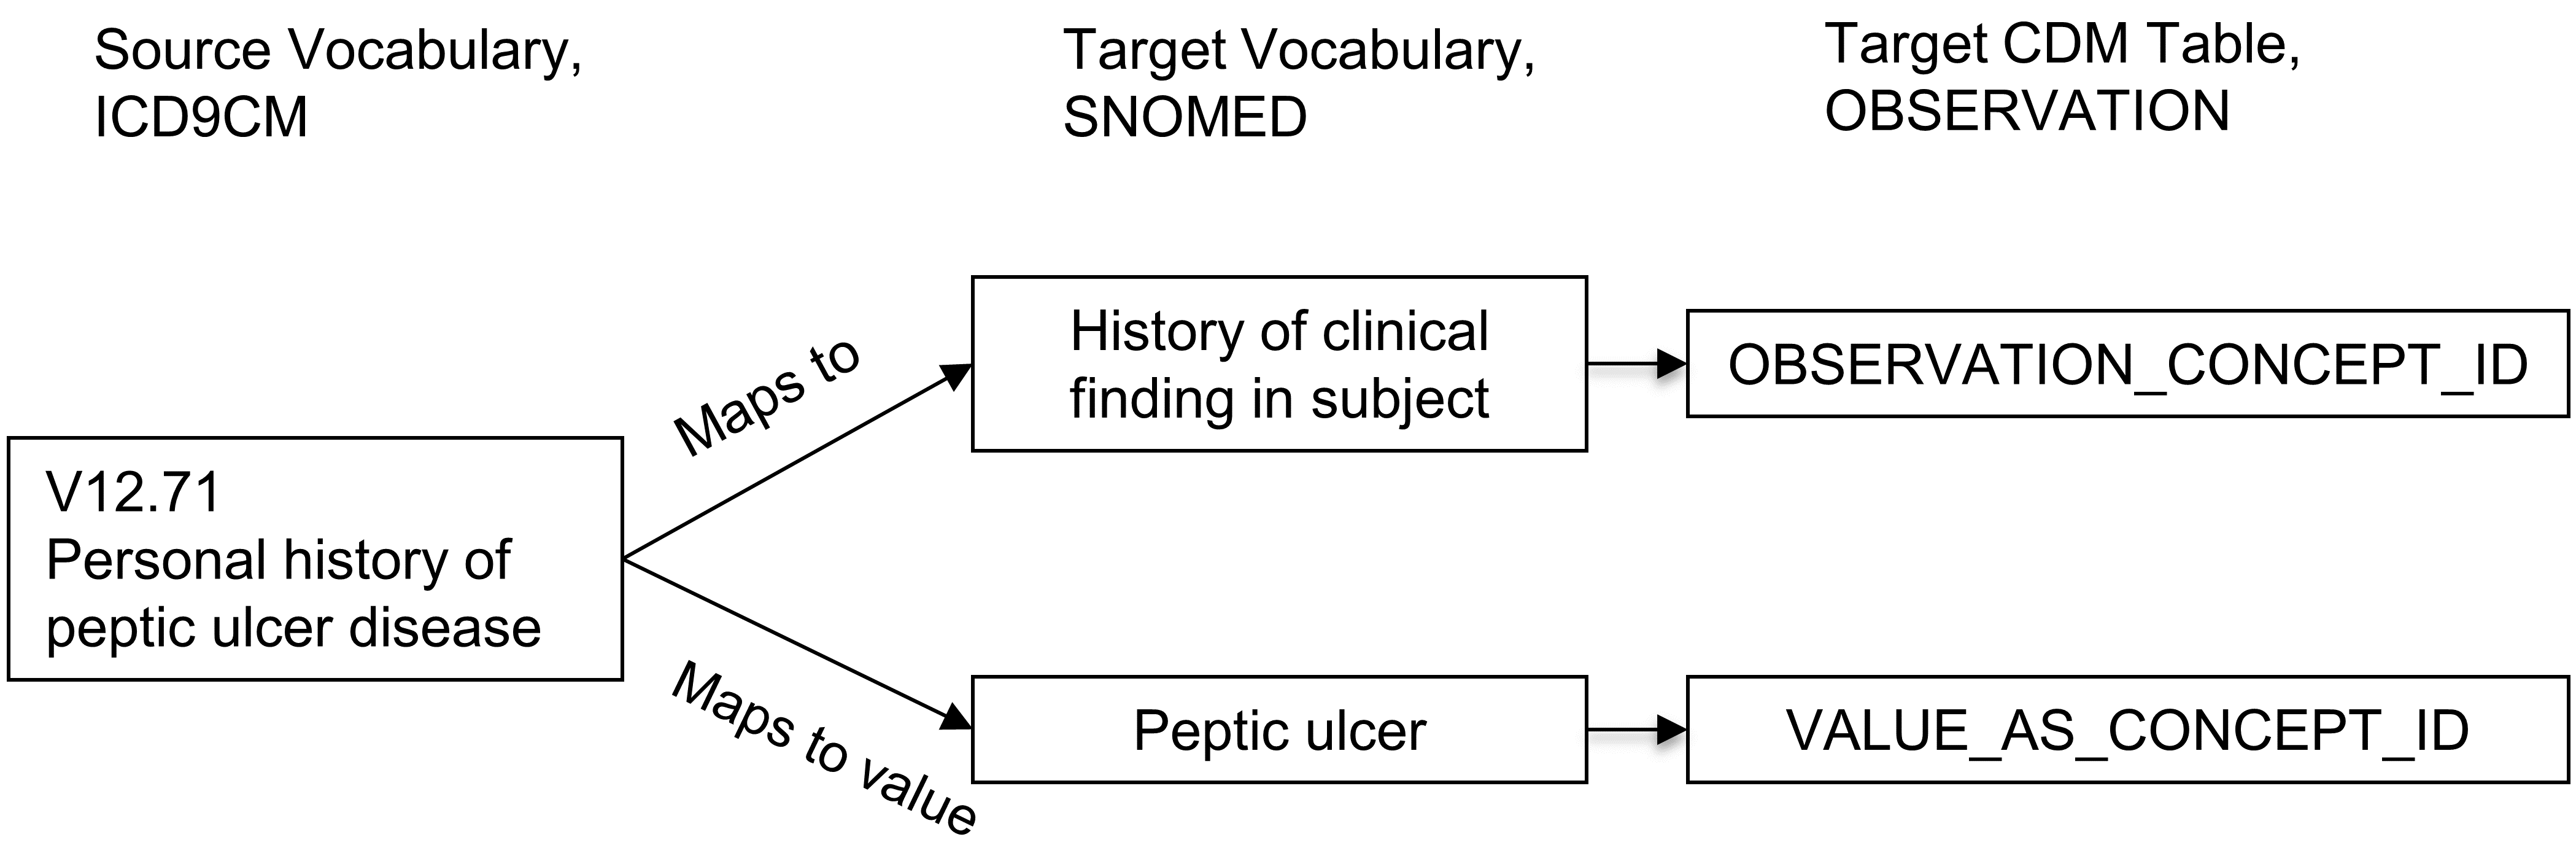
\includegraphics[width=1\linewidth]{images/StandardizedVocabularies/conceptValue} 

}

\caption{One-to-many mapping between source concept and Standard Concepts. A pre-coordinated concept is split into two concepts, one of which is the attribute (here history of clinical finding) and the other one is the value (peptic ulcer). While "Maps to" relationship will map to concepts of the measurement or observation domains, the ‘Maps to value" concepts have no domain restriction.}\label{fig:conceptValue}
\end{figure}

Mapping of concepts is another central feature of the OMOP Standardized
Vocabularies provided for free and supporting the efforts of the
community conducting Network Studies. Mapping relationships are derived
from external sources or maintained manually by the Vocabulary Team.
This means they are not perfect. If you find wrong or objectionable
mapping relationships it is crucial that you report and help improve the
process through a \href{https://forums.ohdsi.org}{Forums} or
\href{https://github.com/OHDSI/CommonDataModel/issues}{CDM issue} post.

A more detailed description of mapping conventions can be found in the
OHDSI Wiki.\footnote{\url{https://www.ohdsi.org/web/wiki/doku.php?id=documentation:vocabulary:mapping}}

\subsection{Hierarchical
Relationships}\label{hierarchical-relationships}

Relationships which indicate a hierarchy are defined through the ``Is
a'' - ``Subsumes'' relationship pair. Hierarchical relationships are
defined such that the child concept has all the attributes of the parent
concept, plus one or more additional attributes or a more precisely
defined attribute. For example, SNOMED 49436004 ``Atrial fibrillation''
is related to SNOMED 17366009 ``Atrial arrhythmia'' through a ``Is a''
relationship. Both concepts have an identical set of attributes except
the type of arrhythmia, which is defined as fibrillation in one but not
the other. Concepts can have more than one parent and more than one
child concept. In this example, SNOMED 49436004 ``Atrial fibrillation''
is also an ``Is a'' to SNOMED 40593004 ``Fibrillation.''
\index{concept!hierarchy}

\subsection{Relationships Between Concepts of Different
Vocabularies}\label{relationships-between-concepts-of-different-vocabularies}

These relationships are typically of the type ``Vocabulary A -
Vocabulary B equivalent'', which is either supplied by the original
source of the vocabulary or is built by the OHDSI Vocabulary team. They
may serve as approximate mappings but often times are less precise than
the better curated mapping relationships. High-quality equivalence
relationships (such as ``Source - RxNorm equivalent'') are always
duplicated by ``Maps to'' relationship.

\subsection{Relationships Between Concepts of the Same
Vocabulary}\label{relationships-between-concepts-of-the-same-vocabulary}

Internal vocabulary relationships are usually supplied by the vocabulary
provider. Full descriptions can be found in the vocabulary documentation
under the individual vocabulary at the OHDSI Wiki.\footnote{\url{https://www.ohdsi.org/web/wiki/doku.php?id=documentation:vocabulary}}

Many of these define relationships between clinical events and can be
used for information retrieval. For example, disorders of the urethra
can be found by following the ``Finding site of'' relationship (see
Table \ref{tab:findingSite}):

\begin{longtable}[]{@{}ll@{}}
\caption{\label{tab:findingSite} ``Finding site of'' relationship of the
``Urethra,'' indicating conditions that are situated all in the this
anatomical structure.}\tabularnewline
\toprule
CONCEPT\_ID\_1 & CONCEPT\_ID\_2\tabularnewline
\midrule
\endfirsthead
\toprule
CONCEPT\_ID\_1 & CONCEPT\_ID\_2\tabularnewline
\midrule
\endhead
4000504 ``Urethra part'' & 36713433 ``Partial duplication of
urethra''\tabularnewline
4000504 ``Urethra part'' & 433583 ``Epispadias''\tabularnewline
4000504 ``Urethra part'' & 443533 ``Epispadias, male''\tabularnewline
4000504 ``Urethra part'' & 4005956 ``Epispadias, female''\tabularnewline
\bottomrule
\end{longtable}

The quality and comprehensiveness of these relationships varies
depending on the quality in the original vocabulary. Generally,
vocabularies that are used to draw Standard Concepts from, such as
SNOMED, are chosen for the reason of their better curation and therefore
tend to have higher quality internal relationships as well.

\section{Hierarchy}\label{conceptAncestor}

Within a domain, standard and classification concepts are organized in a
hierarchical structure and stored in the CONCEPT\_ANCESTOR table. This
allows querying and retrieving concepts and all their hierarchical
descendants. These descendants have the same attributes as their
ancestor, but also additional or more defined ones.

The CONCEPT\_ANCESTOR table is built automatically from the
CONCEPT\_RELATIONSHIP table traversing all possible concepts connected
through hierarchical relationships. These are the ``Is a'' -
``Subsumes'' pairs (see Figure \ref{fig:conceptAncestor}), and other
relationships connecting hierarchies across vocabularies. The choice
whether a relationship participates in the hierarchy constructor is
defined for each relationship ID by the flag DEFINES\_ANCESTRY in the
RELATIONSHIP reference table.







\begin{figure}

{\centering 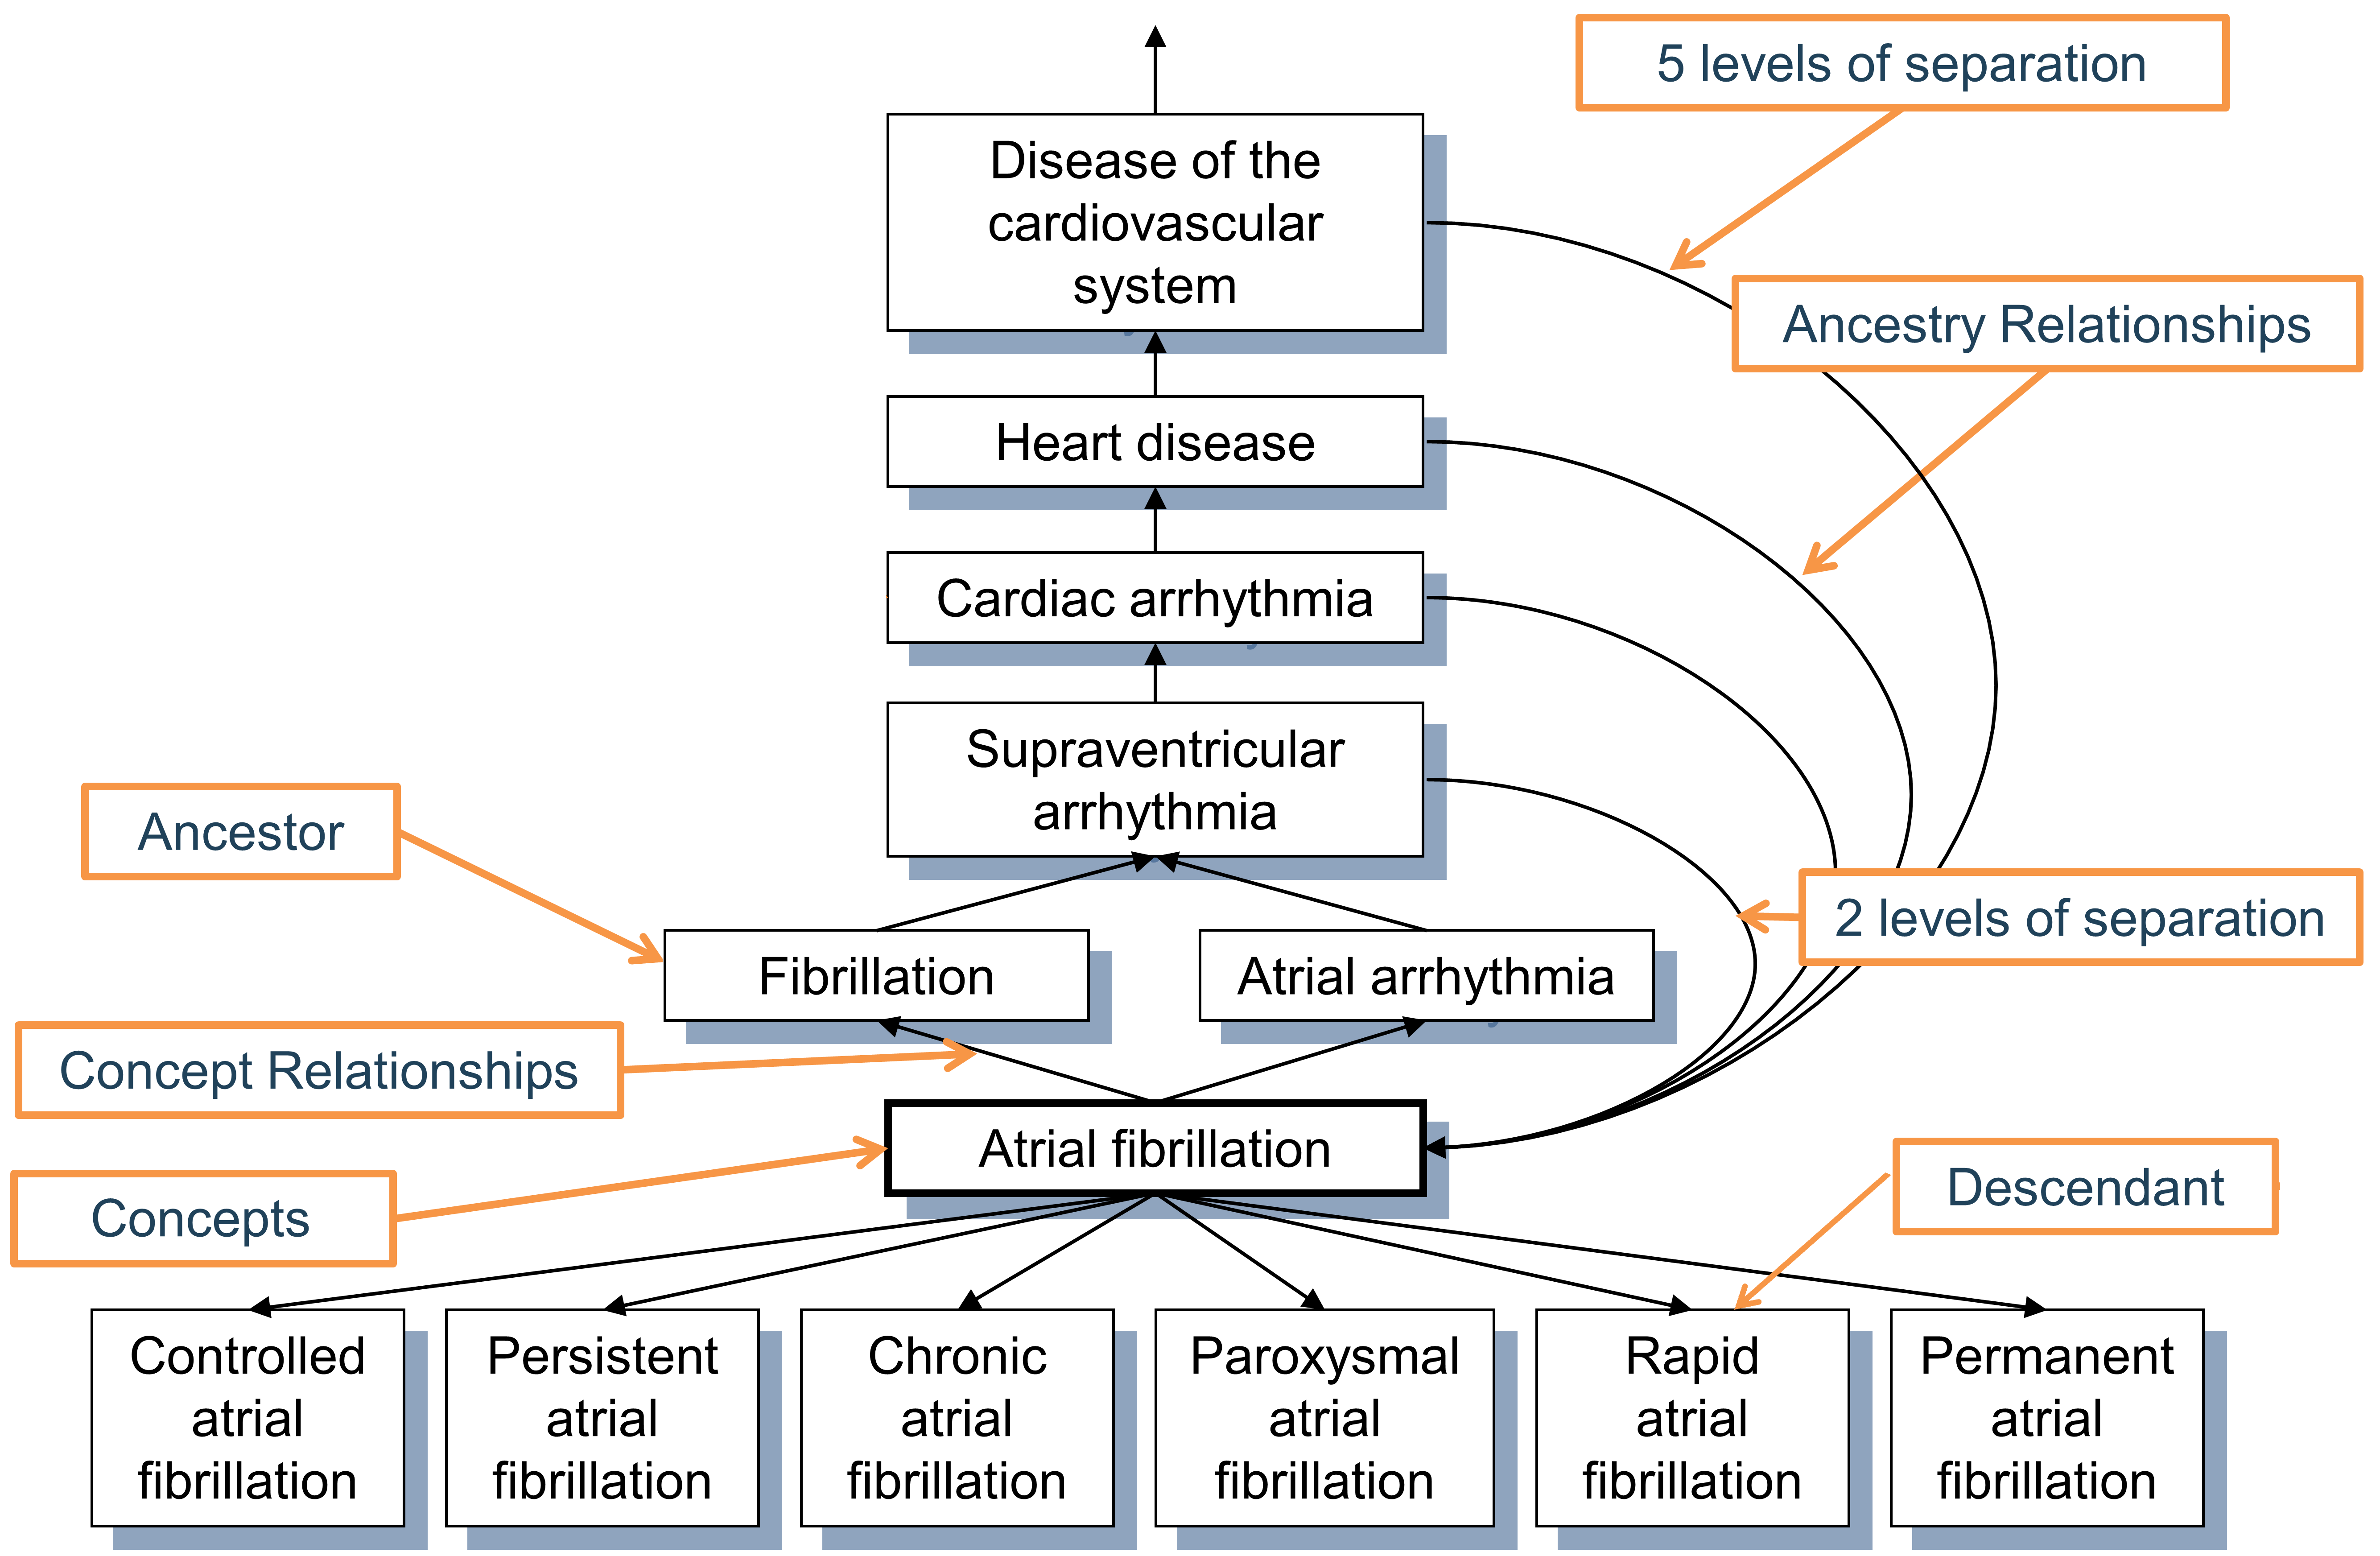
\includegraphics[width=1\linewidth]{images/StandardizedVocabularies/conceptAncestor} 

}

\caption{Hierarchy of the condition ``Atrial fibrillation.'' First
degree ancestry is defined through ``Is a'' and ``Subsumes''
relationships, while all higher degree relations are inferred and stored
in the CONCEPT\_ANCESTOR table. Each concept is also its own descendant
with both levels of separation equal to 0. \index{concept!ancestor}}\label{fig:conceptAncestor}
\end{figure}

The ancestral degree, or the number of steps between ancestor and
descendant, is captured in the MIN\_LEVELS\_OF\_SEPARATION and
MAX\_LEVELS\_OF\_SEPARATION fields, defining the shortest or longest
possible connection. Not all hierarchical relationships contribute
equally to the levels-of-separation calculation. A step counted for the
degree is determined by the IS\_HIERARCHICAL flag in the RELATIONSHIP
reference table for each relationship ID.

At the moment, a high-quality comprehensive hierarchy exists only for
two domains: drug and condition. Procedure, measurement and observation
domains are only partially covered and in the process of construction.
The ancestry is particularly useful for the drug domain as it allows
browsing all drugs with a given ingredient or members of drug classes
irrespective of the country of origin, brand name or other attributes.

\section{Internal Reference Tables}\label{internal-reference-tables}

DOMAIN\_ID, VOCABULARY\_ID, CONCEPT\_CLASS\_ID (all in CONCEPT records)
and CONCEPT\_RELATIONSHIP\_ID (in CONCEPT\_RELATIONSHIP) are all
controlled by their own vocabularies. They are defined in the four
reference tables DOMAIN, VOCABULARY, CONCEPT\_CLASS and RELATIONSHIP,
containing the *\_ID fields as primary keys, a more detailed *\_NAME
field and a *\_CONCEPT\_ID field with a reference back to the CONCEPT
table, which contains a concept for each of the reference table records.
The purpose of these duplicate records is to support an information
model allowing for automatic navigation engines.

The VOCABULARY table also contains the VOCABULARY\_REFERENCE and
VOCABULARY\_VERSION fields referring to the source and version of the
original vocabulary. The RELATIONSHIP table has the additional fields
DEFINES\_ANCESTRY, IS\_HIERARCHICAL and REVERSE\_RELATIONSHIP\_ID. The
latter defines the counter relationship ID for a pair of relationships.

\section{Special Situations}\label{specialSituations}

\subsection{Gender}\label{gender}

Gender in the OMOP CDM and Standardized Vocabularies denotes the
biological sex at birth. Often, questions are posed how to define
alternative genders. These use cases have to be covered through records
in the OBSERVATION table, where the self-defined gender of a person is
stored (if the data asset contains such information).

\subsection{Race and Ethnicity}\label{race-and-ethnicity}

These follow the definitions of how the US government defines this.
Ethnicity is a differentiation of Hispanic or non-Hispanic populations,
which can have any race. Race is divided into the common 5 top races,
which have ethnicities as their hierarchical descendants. Mixed races
are not included.

\subsection{Diagnostic Coding Schemes and OMOP
Conditions}\label{diagnostic-coding-schemes-and-omop-conditions}

Commonly used coding schemes such as ICD-9 or ICD-10 define more or less
well-defined diagnoses based on a proper diagnostic work-up. The
condition domain is not identical with this semantic space, but
partially overlapping. For example, conditions also contain signs and
symptoms that are recorded before a diagnosis is derived, and ICD codes
contain concepts that belong to other domains (e.g.~procedures).

\subsection{Procedure Coding Systems}\label{procedure-coding-systems}

Similarly, coding schemes like HCPCS and CPT4 are thought to be listings
of medical procedures. In reality, they are more like a menu of
justifications for payment for medical service. Many of these services
are subsumed under the procedure domain, but many concepts fall outside
this realm.

\subsection{Devices}\label{devices}

Device concepts have no standardized coding scheme that could be used to
source Standard Concepts. In many source data, devices are not even
coded or contained in an external coding scheme. For this same reason,
there is currently no hierarchical system available.

\subsection{Visits and Services}\label{visits-and-services}

Visits concepts define the nature of healthcare encounters. In many
source systems they are called Place of Service, denoting some
organization or physical structure, such as a hospital. In others, they
are called services. These also differ between countries, and their
definition is hard to obtain. Care sites are often specializing on one
of few visits (XYZ Hospital), but still should not be defined by them
(even in XYZ hospital patients might encounter non-hospital visits).

\subsection{Providers and Specialties}\label{providers-and-specialties}

Any human provider is defined in the provider domain. These can be
medical professionals such as doctors and nurses, but also non-medical
providers like optometrists or shoemakers. Specialties are descendants
of the provider ``Physician.'' Care Sites cannot carry a specialty, even
though they are often defined by the specialty of their main staff
(``Surgical department'').

\subsection{Therapeutic Areas With Special
Requirements}\label{therapeutic-areas-with-special-requirements}

The Standardized Vocabularies cover all aspects of healthcare in a
comprehensive fashion. However, some therapeutic areas have special
needs and require special vocabularies. Examples are oncology,
radiology, and genomics. Special OHDSI Working Groups develop these
extensions. As a result, the OMOP Standardized Vocabularies constitutes
an integrated system, where concepts from different origins and purposes
all reside in the same domain-specific hierarchies.

\subsection{Standard Concepts in the Drug Domain}\label{rxNormExtension}

Many concepts of the drug domain are sourced from RxNorm, a publicly
available vocabulary produced by the US National Library of Medicine.
However, drugs outside the US may or may not be covered, depending on
whether or not the combination of ingredient, form and strength is
marketed in the US. Drugs that are not on the US market are added by the
OHDSI Vocabulary Team under a vocabulary called
\href{https://www.ohdsi.org/web/wiki/doku.php?id=documentation:vocabulary:rxnorm_extension}{RxNorm
Extension}, which is the only large domain vocabulary produced by OHDSI.

\subsection{Flavors of NULL}\label{flavors-of-null}

Many vocabularies contain codes about absence of information. For
example, of the five gender concepts 8507 ``Male,'' 8532 ``Female,''
8570 ``Ambiguous,'' 8551 ``Unknown,'' and 8521 ``Other'', only the first
two are Standard, and the other three are source concepts with no
mapping. In the Standardized Vocabularies, there is no distinction made
why a piece of information is not available; it might be because of an
active withdrawal of information by the patient, a missing value, a
value that is not defined or standardized in some way, or the absence of
a mapping record in CONCEPT\_RELATIONSHIP. Any such concept is not
mapped, which corresponds to a default mapping to the Standard Concept
with the concept ID = 0.

\section{Summary}\label{summary-3}

\BeginKnitrBlock{rmdsummary}
\begin{itemize}
\tightlist
\item
  All events and administrative facts are represented in the OMOP
  Standardized Vocabularies as concepts, concept relationships, and
  concept ancestor hierarchy.
\item
  Most of these are adopted from existing coding schemes or
  vocabularies, while some of them are curated de-novo by the OHDSI
  Vocabulary Team.
\item
  All concepts are assigned a domain, which controls where the fact
  represented by the concept is stored in the CDM.
\item
  Concepts of equivalent meaning in different vocabularies are mapped to
  one of them, which is designated the Standard Concept. The others are
  source concepts.
\item
  Mapping is done through the concept relationships ``Maps to'' and
  ``Maps to value''.
\item
  There is an additional class of concepts called classification
  concepts, which are non-standard, but in contrast to source concepts
  they participate in the hierarchy.
\item
  Concepts have a life-cycle over time.
\item
  Concepts within a domain are organized into hierarchies. The quality
  of the hierarchy differs between domains, and the completion of the
  hierarchy system is an ongoing task.
\item
  You are strongly encouraged to engage with the community if you
  believe you found a mistake or inaccuracy.
\end{itemize}
\EndKnitrBlock{rmdsummary}

\section{Exercises}\label{exercises-1}

\subsubsection*{Prerequisites}\label{prerequisites-2}
\addcontentsline{toc}{subsubsection}{Prerequisites}

For these first exercises you will need to look up concepts in the
Standardized Vocabularies, which can be done through ATHENA\footnote{\url{http://athena.ohdsi.org/}}
or ATLAS.\footnote{\url{http://atlas-demo.ohdsi.org}}

\BeginKnitrBlock{exercise}
\protect\hypertarget{exr:exerciseVocab1}{}{\label{exr:exerciseVocab1} }What
is the Standard Concept ID for ``Gastrointestinal hemorrhage''?
\EndKnitrBlock{exercise}

\BeginKnitrBlock{exercise}
\protect\hypertarget{exr:exerciseVocab2}{}{\label{exr:exerciseVocab2} }Which
ICD-10CM codes map to the Standard Concept for ``Gastrointestinal
hemorrhage''? Which ICD-9CM codes map to this Standard Concept?
\EndKnitrBlock{exercise}

\BeginKnitrBlock{exercise}
\protect\hypertarget{exr:exerciseVocab3}{}{\label{exr:exerciseVocab3} }What
are the MedDRA preferred terms that are equivalent to the Standard
Concept for ``Gastrointestinal hemorrhage''?
\EndKnitrBlock{exercise}

Suggested answers can be found in Appendix \ref{Vocabanswers}.

\chapter{Extract Transform Load}\label{ExtractTransformLoad}

\emph{Chapter leads: Clair Blacketer \& Erica Voss}

\section{Introduction}\label{introduction-1}

In order to get from the native/raw data to the OMOP Common Data Model
(CDM) we have to create an extract, transform, and load (ETL) process.
This process should restructure the data to the CDM, and add mappings to
the Standardized Vocabularies, and is typically implemented as a set of
automated scripts, for example SQL scripts. It is important that this
ETL process is repeatable, so that it can be rerun whenever the source
data is refreshed. \index{ETL|see {extract, transform and load (ETL)}}
\index{raw data} \index{native data|see {raw data}}
\index{source data|see{raw data}}

Creating an ETL is usually a large undertaking. Over the years, we have
developed best practices, consisting of four major steps:

\begin{enumerate}
\def\labelenumi{\arabic{enumi}.}
\tightlist
\item
  Data experts and CDM experts together design the ETL.
\item
  People with medical knowledge create the code mappings.
\item
  A technical person implements the ETL.
\item
  All are involved in quality control.
\end{enumerate}

In this chapter we will discuss each of these steps in detail. Several
tools have been developed by the OHDSI community to support some of
these steps, and these will be discussed as well. We close this chapter
with a discussion of CDM and ETL maintenance.

\section{Step 1: Design the ETL}\label{step-1-design-the-etl}

It is important to clearly separate the design of the ETL from the
implementation of the ETL. Designing the ETL requires extensive
knowledge of both the source data, as well as the CDM. Implementing the
ETL on the other hand typically relies mostly on technical expertise on
how to make the ETL computationally efficient. If we try to do both at
once, we are likely to get stuck in nitty-gritty details, while we
should be focusing on the overall picture.

Two closely-integrated tools have been developed to support the ETL
design process: White Rabbit, and Rabbit-in-a-Hat.

\subsection{White Rabbit}\label{white-rabbit}

To initiate an ETL process on a database you need to understand your
data, including the tables, fields, and content. This is where the
\href{https://github.com/OHDSI/WhiteRabbit}{White Rabbit} tool comes in.
White Rabbit is a software tool to help prepare for ETLs of longitudinal
healthcare databases into the
\href{https://github.com/OHDSI/CommonDataModel}{OMOP CDM}. White Rabbit
scans your data and creates a report containing all the information
necessary to begin designing the ETL. All source code and installation
instructions, as well as a link to the manual, are available on
GitHub.\footnote{\url{https://github.com/OHDSI/WhiteRabbit}.}
\index{White Rabbit} \index{data profiling|see {White Rabbit}}

\subsubsection*{Scope and Purpose}\label{scope-and-purpose}
\addcontentsline{toc}{subsubsection}{Scope and Purpose}

White Rabbit's main function is to perform a scan of the source data,
providing detailed information on the tables, fields, and values that
appear in a field. The source data can be in comma-separated text files,
or in a database (MySQL, SQL Server, Oracle, PostgreSQL, Microsoft APS,
Microsoft Access, Amazon RedShift). The scan will generate a report that
can be used as a reference when designing the ETL, for instance by using
it in conjunction with the Rabbit-In-a-Hat tool. White Rabbit differs
from standard data profiling tools in that it attempts to prevent the
display of personally identifiable information (PII) data values in the
generated output data file.

\subsubsection*{Process Overview}\label{process-overview}
\addcontentsline{toc}{subsubsection}{Process Overview}

The typical sequence for using the software to scan source data:

\begin{enumerate}
\def\labelenumi{\arabic{enumi}.}
\tightlist
\item
  Set working folder, the location on the local desktop computer where
  results will be exported.
\item
  Connect to the source database or CSV text file and test connection.
\item
  Select the tables of interest for the scan and scan the tables.
\item
  White Rabbit creates an export of information about the source data.
\end{enumerate}

\subsubsection*{Setting a Working
Folder}\label{setting-a-working-folder}
\addcontentsline{toc}{subsubsection}{Setting a Working Folder}

After downloading and installing the White Rabbit application, the first
thing you need to do is set a working folder. Any files that White
Rabbit creates will be exported to this local folder. Use the ``Pick
Folder'' button shown in Figure \ref{fig:WhiteRabbitLocation} to
navigate in your local environment where you would like the scan
document to go.

\begin{figure}

{\centering 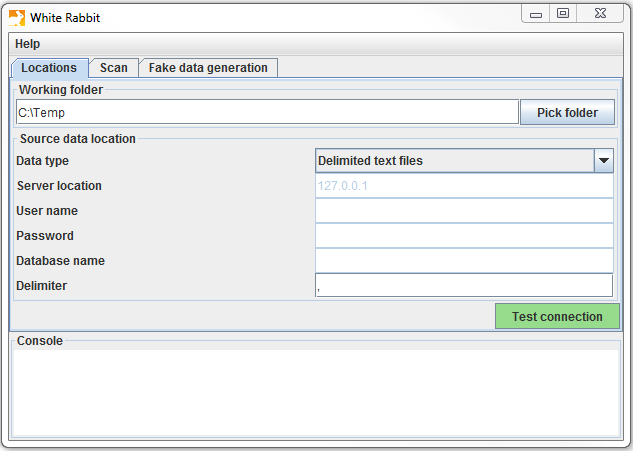
\includegraphics[width=1\linewidth]{images/ExtractTransformLoad/WhiteRabbitLocation} 

}

\caption{The "Pick Folder" button allows the specification of a working folder for the White Rabbit application.}\label{fig:WhiteRabbitLocation}
\end{figure}

\subsubsection*{Connection to a
Database}\label{connection-to-a-database}
\addcontentsline{toc}{subsubsection}{Connection to a Database}

White Rabbit supports delimited text files and various database
platforms. Hover the mouse over the various fields to get a description
of what is required. More detailed information can be found in the
manual.

\subsubsection*{Scanning the Tables in a
Database}\label{scanning-the-tables-in-a-database}
\addcontentsline{toc}{subsubsection}{Scanning the Tables in a Database}

After connecting to a database, you can scan the tables contained
therein. A scan generates a report containing information on the source
data that can be used to help design the ETL. Using the Scan tab shown
in Figure \ref{fig:WhiteRabbitAddTables} you can either select
individual tables in the selected source database by clicking on ``Add''
(Ctrl + mouse click), or automatically select all tables in the database
by clicking on ``Add all in DB''.

\begin{figure}

{\centering 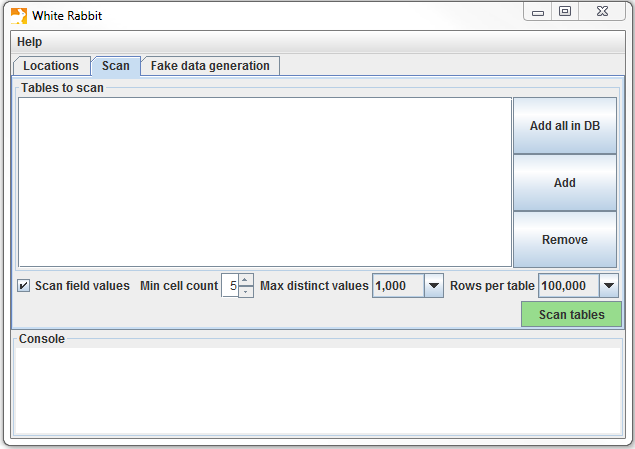
\includegraphics[width=1\linewidth]{images/ExtractTransformLoad/WhiteRabbitAddTables} 

}

\caption{White Rabbit Scan tab.}\label{fig:WhiteRabbitAddTables}
\end{figure}

There are a few setting options as well with the scan:

\begin{itemize}
\tightlist
\item
  Checking the ``Scan field values'' tells WhiteRabbit that you would
  like to investigate which values appear in the columns.
\item
  ``Min cell count'' is an option when scanning field values. By
  default, this is set to 5, meaning values in the source data that
  appear less than 5 times will not appear in the report. Individual
  data sets may have their own rules about what this minimum cell count
  can be.
\item
  ``Rows per table'' is an option when scanning field values. By
  default, White Rabbit will scan 100,000 randomly selected rows in the
  table.
\end{itemize}

Once all settings are completed, press the ``Scan tables'' button. After
the scan is completed the report will be written to the working folder.

\subsubsection*{Interpreting the Scan
Report}\label{interpreting-the-scan-report}
\addcontentsline{toc}{subsubsection}{Interpreting the Scan Report}

Once the scan is complete, an Excel file is generated in the selected
folder with one tab present for each table scanned as well as an
overview tab. The overview tab lists all tables scanned, each field in
each table, the data type of each field, the maximum length of the
field, the number of rows in the table, the number of rows scanned, and
how often each field was found to be empty. Figure
\ref{fig:ScanOverviewTab}. shows an example overview tab.

\begin{figure}

{\centering 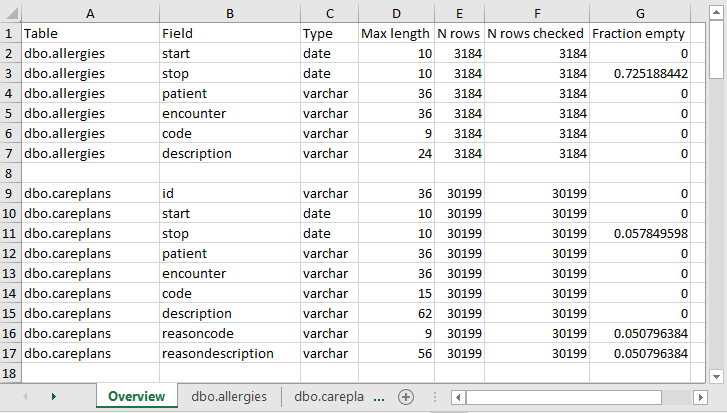
\includegraphics[width=1\linewidth]{images/ExtractTransformLoad/ScanOverviewTab} 

}

\caption{Example overview tab from a scan report.}\label{fig:ScanOverviewTab}
\end{figure}

The tabs for each of the tables show each field, the values in each
field, and the frequency of each value. Each source table column will
generate two columns in the Excel. One column will list all distinct
values that have a ``Min cell count'' greater than what was set at time
of the scan. If a list of unique values was truncated, the last value in
the list will be ``List truncated''; this indicates that there are one
or more additional unique source values that appear less than the number
entered in the ``Min cell count''. Next to each distinct value will be a
second column that contains the frequency (the number of times that
value occurs in the sample). These two columns (distinct values and
frequency) will repeat for all the source columns in the table profiled
in the workbook.

\begin{figure}

{\centering 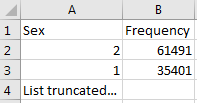
\includegraphics[width=0.3\linewidth]{images/ExtractTransformLoad/ScanSex} 

}

\caption{Example values for a single column.}\label{fig:scanSex}
\end{figure}

The report is powerful in understanding your source data by highlighting
what exists. For example, if the results shown in Figure
\ref{fig:scanSex} were given back on the ``Sex'' column within one of
the tables scanned, we can see that there were two common values (1 and
2) that appeared 61,491 and 35,401 times respectively. White Rabbit will
not define 1 as male and 2 as female; the data holder will typically
need to define source codes unique to the source system. However, these
two values (1 \& 2) are not the only values present in the data because
we see this list was truncated. These other values appear with very low
frequency (defined by ``Min cell count'') and often represent incorrect
or highly suspicious values. When generating an ETL we should not only
plan to handle the high-frequency gender concepts 1 and 2 but the other
low-frequency values that exist within this column. For example, if
those lower frequency genders were ``NULL'' we want to make sure the ETL
can handle processing that data and knows what to do in that situation.

\subsection{Rabbit-In-a-Hat}\label{rabbit-in-a-hat}

With the White Rabbit scan in hand, we have a clear picture of the
source data. We also know the full specification of the CDM. Now we need
to define the logic to go from one to the other. This design activity
requires thorough knowledge of both the source data and the CDM. The
Rabbit-in-a-Hat tools that comes with the White Rabbit software is
specifically designed to support a team of experts in these areas. In a
typical setting, the ETL design team sits together in a room, while
Rabbit-in-a-Hat is projected on a screen. In a first round, the
table-to-table mappings can be collaboratively decided, after which
field-to-field mappings can be designed, while defining the logic by
which values will be transformed. \index{Rabbit-In-A-Hat}
\index{ETL design|see {Rabbit-In-A-Hat}}

\subsubsection*{Scope and Purpose}\label{scope-and-purpose-1}
\addcontentsline{toc}{subsubsection}{Scope and Purpose}

Rabbit-In-a-Hat is designed to read and display a White Rabbit scan
document. White Rabbit generates information about the source data while
Rabbit-In-a-Hat uses that information and through a graphical user
interface to allow a user to connect source data to tables and columns
within the CDM. Rabbit-In-a-Hat generates documentation for the ETL
process, it does not generate code to create an ETL.

\subsubsection*{Process Overview}\label{process-overview-1}
\addcontentsline{toc}{subsubsection}{Process Overview}

The typical sequence for using this software to generate documentation
of an ETL:

\begin{enumerate}
\def\labelenumi{\arabic{enumi}.}
\tightlist
\item
  Scanned results from WhiteRabbit completed.
\item
  Open scanned results; interface displays source tables and CDM tables.
\item
  Connect source tables to CDM tables where the source table provides
  information for that corresponding CDM table.
\item
  For each source table to CDM table connection, further define the
  connection with source column to CDM column detail.
\item
  Save Rabbit-In-a-Hat work and export to a MS Word document.
\end{enumerate}

\subsubsection*{Writing ETL Logic}\label{writing-etl-logic}
\addcontentsline{toc}{subsubsection}{Writing ETL Logic}

Once you have opened your White Rabbit scan report in Rabbit-In-a-Hat
you are ready to begin designing and writing the logic for how to
convert the source data to the OMOP CDM. As an example, the next few
sections will depict how some of the tables in the Synthea\footnote{Synthea\textsuperscript{TM}
  is a patient generator that aims to model real patients. Data are
  created based on parameters passed to the application.The structure of
  the data can be found here:
  \url{https://github.com/synthetichealth/synthea/wiki}.} database might
look during conversion.

\subsubsection*{General Flow of an ETL}\label{general-flow-of-an-etl}
\addcontentsline{toc}{subsubsection}{General Flow of an ETL}

Since the CDM is a person-centric model it is always a good idea to
start mapping the PERSON table first. Every clinical event table
(CONDITION\_OCCURRENCE, DRUG\_EXPOSURE, PROCEDURE\_OCCURRENCE, etc.)
refers to the PERSON table by way of the person\_id so working out the
logic for the PERSON table first makes it easier later on. After the
PERSON table a good rule of thumb is to convert the OBSERVATION\_PERIOD
table next. Each person in a CDM database should have at least one
OBSERVATION\_PERIOD and, generally, most events for a person fall within
this timeframe. Once the PERSON and OBSERVATION\_PERIOD tables are done
the dimensional tables like PROVIDER, CARE\_SITE, and LOCATION are
typically next. The final table logic that should be worked out prior to
the clinical tables is VISIT\_OCCURRENCE. Often this is the most
complicated logic in the entire ETL and it is some of the most crucial
since most events that occur during the course of a person's patient
journey will happen during visits. Once those tables are finished it is
your choice which CDM tables to map and in which order.

\begin{figure}

{\centering 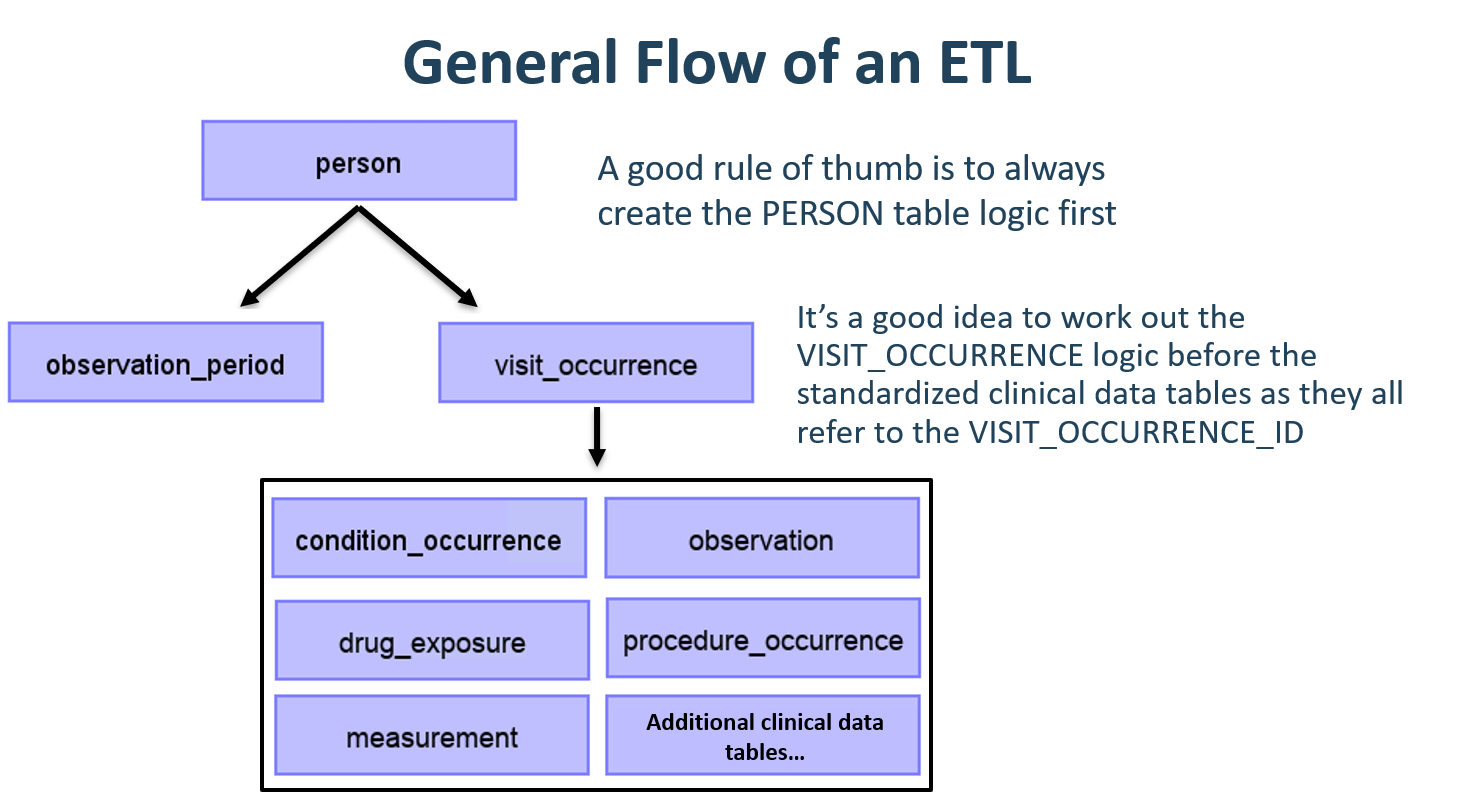
\includegraphics[width=1\linewidth]{images/ExtractTransformLoad/flowOfEtl} 

}

\caption{General flow of an ETL and which tables to map first.}\label{fig:etlFlow}
\end{figure}

It is often the case that, during CDM conversion, you will need to make
provisions for intermediate tables. This could be for assigning the
correct VISIT\_OCCURRENCE\_IDs to events, or for mapping source codes to
standard concepts (doing this step on the fly is often very slow).
Intermediate tables are 100\% allowed and encouraged. What is
discouraged is the persistence and reliance on these intermediate tables
once the conversion is complete.

\subsubsection*{Mapping Example: Person
Table}\label{mapping-example-person-table}
\addcontentsline{toc}{subsubsection}{Mapping Example: Person Table}

The Synthea data structure contains 20 columns in the patients table but
not all were needed to populate the PERSON table, as seen in Figure
\ref{fig:syntheaPerson}. This is very common and should not be cause for
alarm. In this example many of the data points in the Synthea patients
table that were not used in the CDM PERSON table were additional
identifiers like patient name, driver's license number, and passport
number.

\begin{figure}

{\centering 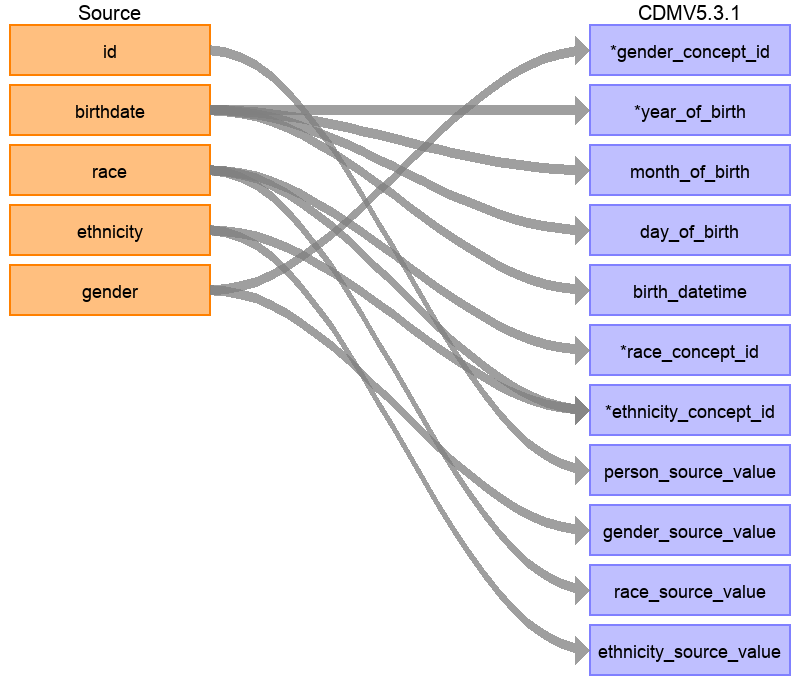
\includegraphics[width=1\linewidth]{images/ExtractTransformLoad/syntheaPersonTable} 

}

\caption{Mapping of Synthea Patients table to CDM PERSON table.}\label{fig:syntheaPerson}
\end{figure}

Table \ref{tab:syntheaEtlPerson} below shows the logic that was imposed
on the Synthea patients table to convert it to the CDM PERSON table. The
`Destination Field' discusses where in the CDM data is being mapped to.
The `Source field' highlights the column from the source table (in this
case patients) that will be used to populate the CDM column. Finally,
the `Logic \& comments' column gives explanations for the logic.

\begin{longtable}[]{@{}lll@{}}
\caption{\label{tab:syntheaEtlPerson} ETL logic to convert the Synthea
Patients table to CDM PERSON table.}\tabularnewline
\toprule
\begin{minipage}[b]{0.28\columnwidth}\raggedright\strut
Destination Field\strut
\end{minipage} & \begin{minipage}[b]{0.13\columnwidth}\raggedright\strut
Source field\strut
\end{minipage} & \begin{minipage}[b]{0.50\columnwidth}\raggedright\strut
Logic \& comments\strut
\end{minipage}\tabularnewline
\midrule
\endfirsthead
\toprule
\begin{minipage}[b]{0.28\columnwidth}\raggedright\strut
Destination Field\strut
\end{minipage} & \begin{minipage}[b]{0.13\columnwidth}\raggedright\strut
Source field\strut
\end{minipage} & \begin{minipage}[b]{0.50\columnwidth}\raggedright\strut
Logic \& comments\strut
\end{minipage}\tabularnewline
\midrule
\endhead
\begin{minipage}[t]{0.28\columnwidth}\raggedright\strut
PERSON\_ID\strut
\end{minipage} & \begin{minipage}[t]{0.13\columnwidth}\raggedright\strut
\strut
\end{minipage} & \begin{minipage}[t]{0.50\columnwidth}\raggedright\strut
Autogenerate. The PERSON\_ID will be generated at the time of
implementation. This is because the id value from the source is a
varchar value while the PERSON\_ID is an integer. The id field from the
source is set as the PERSON\_SOURCE\_VALUE to preserve that value and
allow for error-checking if necessary.\strut
\end{minipage}\tabularnewline
\begin{minipage}[t]{0.28\columnwidth}\raggedright\strut
GENDER\_CONCEPT\_ID\strut
\end{minipage} & \begin{minipage}[t]{0.13\columnwidth}\raggedright\strut
gender\strut
\end{minipage} & \begin{minipage}[t]{0.50\columnwidth}\raggedright\strut
When gender = `M' then set GENDER\_CONCEPT\_ID to 8507, when gender =
`F' then set to 8532. Drop any rows with missing/unknown gender. These
two concepts were chosen as they are the only two standard concepts in
the gender domain. The choice to drop patients with unknown genders
tends to be site-based, though it is recommended they are removed as
people without a gender are excluded from analyses.\strut
\end{minipage}\tabularnewline
\begin{minipage}[t]{0.28\columnwidth}\raggedright\strut
YEAR\_OF\_BIRTH\strut
\end{minipage} & \begin{minipage}[t]{0.13\columnwidth}\raggedright\strut
birthdate\strut
\end{minipage} & \begin{minipage}[t]{0.50\columnwidth}\raggedright\strut
Take year from birthdate\strut
\end{minipage}\tabularnewline
\begin{minipage}[t]{0.28\columnwidth}\raggedright\strut
MONTH\_OF\_BIRTH\strut
\end{minipage} & \begin{minipage}[t]{0.13\columnwidth}\raggedright\strut
birthdate\strut
\end{minipage} & \begin{minipage}[t]{0.50\columnwidth}\raggedright\strut
Take month from birthdate\strut
\end{minipage}\tabularnewline
\begin{minipage}[t]{0.28\columnwidth}\raggedright\strut
DAY\_OF\_BIRTH\strut
\end{minipage} & \begin{minipage}[t]{0.13\columnwidth}\raggedright\strut
birthdate\strut
\end{minipage} & \begin{minipage}[t]{0.50\columnwidth}\raggedright\strut
Take day from birthdate\strut
\end{minipage}\tabularnewline
\begin{minipage}[t]{0.28\columnwidth}\raggedright\strut
BIRTH\_DATETIME\strut
\end{minipage} & \begin{minipage}[t]{0.13\columnwidth}\raggedright\strut
birthdate\strut
\end{minipage} & \begin{minipage}[t]{0.50\columnwidth}\raggedright\strut
With midnight as time 00:00:00. Here, the source did not supply a time
of birth so the choice was made to set it at midnight.\strut
\end{minipage}\tabularnewline
\begin{minipage}[t]{0.28\columnwidth}\raggedright\strut
RACE\_CONCEPT\_ID\strut
\end{minipage} & \begin{minipage}[t]{0.13\columnwidth}\raggedright\strut
race\strut
\end{minipage} & \begin{minipage}[t]{0.50\columnwidth}\raggedright\strut
When race = `WHITE' then set as 8527, when race = `BLACK' then set as
8516, when race = `ASIAN' then set as 8515, otherwise set as 0. These
concepts were chosen because they are the standard concepts belonging to
the race domain that most closely align with the race categories in the
source.\strut
\end{minipage}\tabularnewline
\begin{minipage}[t]{0.28\columnwidth}\raggedright\strut
ETHNICITY\_ CONCEPT\_ID\strut
\end{minipage} & \begin{minipage}[t]{0.13\columnwidth}\raggedright\strut
race ethnicity\strut
\end{minipage} & \begin{minipage}[t]{0.50\columnwidth}\raggedright\strut
When race = `HISPANIC', or when ethnicity in (`CENTRAL\_AMERICAN',
`DOMINICAN', `MEXICAN', `PUERTO\_RICAN', `SOUTH\_AMERICAN') then set as
38003563, otherwise set as 0. This is a good example of how multiple
source columns can contribute to one CDM column. In the CDM ethnicity is
represented as either Hispanic or not Hispanic so values from both the
source column race and source column ethnicity will determine this
value.\strut
\end{minipage}\tabularnewline
\begin{minipage}[t]{0.28\columnwidth}\raggedright\strut
LOCATION\_ID\strut
\end{minipage} & \begin{minipage}[t]{0.13\columnwidth}\raggedright\strut
\strut
\end{minipage} & \begin{minipage}[t]{0.50\columnwidth}\raggedright\strut
\strut
\end{minipage}\tabularnewline
\begin{minipage}[t]{0.28\columnwidth}\raggedright\strut
PROVIDER\_ID\strut
\end{minipage} & \begin{minipage}[t]{0.13\columnwidth}\raggedright\strut
\strut
\end{minipage} & \begin{minipage}[t]{0.50\columnwidth}\raggedright\strut
\strut
\end{minipage}\tabularnewline
\begin{minipage}[t]{0.28\columnwidth}\raggedright\strut
CARE\_SITE\_ID\strut
\end{minipage} & \begin{minipage}[t]{0.13\columnwidth}\raggedright\strut
\strut
\end{minipage} & \begin{minipage}[t]{0.50\columnwidth}\raggedright\strut
\strut
\end{minipage}\tabularnewline
\begin{minipage}[t]{0.28\columnwidth}\raggedright\strut
PERSON\_SOURCE\_ VALUE\strut
\end{minipage} & \begin{minipage}[t]{0.13\columnwidth}\raggedright\strut
id\strut
\end{minipage} & \begin{minipage}[t]{0.50\columnwidth}\raggedright\strut
\strut
\end{minipage}\tabularnewline
\begin{minipage}[t]{0.28\columnwidth}\raggedright\strut
GENDER\_SOURCE\_ VALUE\strut
\end{minipage} & \begin{minipage}[t]{0.13\columnwidth}\raggedright\strut
gender\strut
\end{minipage} & \begin{minipage}[t]{0.50\columnwidth}\raggedright\strut
\strut
\end{minipage}\tabularnewline
\begin{minipage}[t]{0.28\columnwidth}\raggedright\strut
GENDER\_SOURCE\_ CONCEPT\_ID\strut
\end{minipage} & \begin{minipage}[t]{0.13\columnwidth}\raggedright\strut
\strut
\end{minipage} & \begin{minipage}[t]{0.50\columnwidth}\raggedright\strut
\strut
\end{minipage}\tabularnewline
\begin{minipage}[t]{0.28\columnwidth}\raggedright\strut
RACE\_SOURCE\_ VALUE\strut
\end{minipage} & \begin{minipage}[t]{0.13\columnwidth}\raggedright\strut
race\strut
\end{minipage} & \begin{minipage}[t]{0.50\columnwidth}\raggedright\strut
\strut
\end{minipage}\tabularnewline
\begin{minipage}[t]{0.28\columnwidth}\raggedright\strut
RACE\_SOURCE\_ CONCEPT\_ID\strut
\end{minipage} & \begin{minipage}[t]{0.13\columnwidth}\raggedright\strut
\strut
\end{minipage} & \begin{minipage}[t]{0.50\columnwidth}\raggedright\strut
\strut
\end{minipage}\tabularnewline
\begin{minipage}[t]{0.28\columnwidth}\raggedright\strut
ETHNICITY\_ SOURCE\_VALUE\strut
\end{minipage} & \begin{minipage}[t]{0.13\columnwidth}\raggedright\strut
ethnicity\strut
\end{minipage} & \begin{minipage}[t]{0.50\columnwidth}\raggedright\strut
In this case the ETHNICITY\_SOURCE\_VALUE will have more granularity
than the ETHNICITY\_CONCEPT\_ID.\strut
\end{minipage}\tabularnewline
\begin{minipage}[t]{0.28\columnwidth}\raggedright\strut
ETHNICITY\_ SOURCE\_CONCEPT\_ID\strut
\end{minipage} & \begin{minipage}[t]{0.13\columnwidth}\raggedright\strut
\strut
\end{minipage} & \begin{minipage}[t]{0.50\columnwidth}\raggedright\strut
\strut
\end{minipage}\tabularnewline
\bottomrule
\end{longtable}

For more examples on how the Synthea dataset was mapped to the CDM
please see the full specification document.\footnote{\url{https://ohdsi.github.io/ETL-Synthea/}}

\section{Step 2: Create the Code
Mappings}\label{step-2-create-the-code-mappings}

More and more source codes are being added to the OMOP Vocabulary all
the time. This means that the coding systems in the data being
transformed to the CDM may already be included and mapped. Check the
VOCABULARY table in the OMOP Vocabulary to see which vocabularies are
included. To extract the mapping from non-standard source codes
(e.g.~ICD-10CM codes) to standard concepts (e.g.~SNOMED codes), we can
use the records in the CONCEPT\_RELATIONSHIP table having
relationship\_id = ``Maps to''. For example, to find the standard
concept ID for the ICD-10CM code `I21' (``Acute Myocardial
Infarction''), we can use the following SQL:

\begin{Shaded}
\begin{Highlighting}[]
\KeywordTok{SELECT}\NormalTok{ concept_id_2 standard_concept_id}
\KeywordTok{FROM}\NormalTok{ concept_relationship}
\KeywordTok{INNER} \KeywordTok{JOIN}\NormalTok{ concept source_concept}
  \KeywordTok{ON}\NormalTok{ concept_id = concept_id_}\DecValTok{1}
\KeywordTok{WHERE}\NormalTok{ concept_code = }\StringTok{'I21'}
  \KeywordTok{AND}\NormalTok{ vocabulary_id = }\StringTok{'ICD10CM'}
  \KeywordTok{AND}\NormalTok{ relationship_id = }\StringTok{'Maps to'}\NormalTok{; }
\end{Highlighting}
\end{Shaded}

\begin{longtable}[]{@{}r@{}}
\toprule
STANDARD\_CONCEPT\_ID\tabularnewline
\midrule
\endhead
312327\tabularnewline
\bottomrule
\end{longtable}

Unfortunately, sometimes the source data uses coding systems that are
not in the Vocabulary. In this case, a mapping must be created from the
source coding system to the Standard Concepts. Code mapping can be a
daunting task, especially when there are many codes in the source coding
system. There are several things that can be done to make the task
easier:

\begin{itemize}
\tightlist
\item
  Focus on the most frequently used codes. A code that is never used or
  infrequently used is not worth the effort of mapping, since it will
  never be used in a real study.
\item
  Make use of existing information whenever possible. For example, many
  national drug coding systems have been mapped to ATC. Although ATC is
  not detailed enough for many purposes, the concept relationships
  between ATC and RxNorm can be used to make good guesses of what the
  right RxNorm codes are.
\item
  Use Usagi.
\end{itemize}

\subsection{Usagi}\label{usagi}

Usagi is a tool to aid the manual process of creating a code mapping. It
can make suggested mappings based on textual similarity of code
descriptions. If the source codes are only available in a foreign
language, we have found that Google Translate\footnote{\url{https://translate.google.com/}}
often gives surprisingly good translation of the terms into English.
Usagi allows the user to search for the appropriate target concepts if
the automated suggestion is not correct. Finally, the user can indicate
which mappings are approved to be used in the ETL. Usagi is available on
GitHub.\footnote{\url{https://github.com/OHDSI/Usagi}} \index{Usagi}
\index{source code mapping|see {Usagi}}

\subsubsection*{Scope and Purpose}\label{scope-and-purpose-2}
\addcontentsline{toc}{subsubsection}{Scope and Purpose}

Source codes that need mapping are loaded into the Usagi (if the codes
are not in English additional translations columns are needed). A term
similarity approach is used to connect source codes to Vocabulary
concepts. However, these code connections need to be manually reviewed
and Usagi provides an interface to facilitate that. Usagi will only
propose concepts that are marked as Standard concepts in the Vocabulary.

\subsubsection*{Process Overview}\label{process-overview-2}
\addcontentsline{toc}{subsubsection}{Process Overview}

The typical sequence for using this software is:

\begin{enumerate}
\def\labelenumi{\arabic{enumi}.}
\tightlist
\item
  Load codes from your sources system (``source codes'') that you would
  like to map to Vocabulary concepts.
\item
  Usagi will run term similarity approach to map source codes to
  Vocabulary concepts.
\item
  Leverage Usagi interface to check, and where needed, improve suggested
  mappings. Preferably an individual who has experience with the coding
  system and medical terminology should be used for this review.
\item
  Export mapping to the Vocabulary's SOURCE\_TO\_CONCEPT\_MAP.
\end{enumerate}

\subsubsection*{Importing Source Codes into
Usagi}\label{importing-source-codes-into-usagi}
\addcontentsline{toc}{subsubsection}{Importing Source Codes into Usagi}

Export source codes from source system into a CSV or Excel (.xlsx) file.
This should at least have columns containing the source code and an
English source code description, however additional information about
codes can be brought over as well (e.g.~dose unit, or the description in
the original language if translated). In addition to information about
the source codes, the frequency of the code should preferably also be
brought over, since this can help prioritize which codes should receive
the most effort in mapping (e.g.~you can have 1,000 source codes but
only 100 are truly used within the system). If any source code
information needs translating to English, use Google Translate to do
that.

Note: source code extracts should be broken out by domain (i.e.~drugs,
procedures, conditions, observations) and not lumped into one large
file.

Source codes are loaded into Usagi from the File --\textgreater{} Import
codes menu. From here an ``Import codes \ldots{}'' will display as seen
in Figure \ref{fig:usagiImport}. In this figure, the source code terms
were in Dutch and were also translated into English. Usagi will leverage
the English translations to map to the standard vocabulary.

\begin{figure}

{\centering 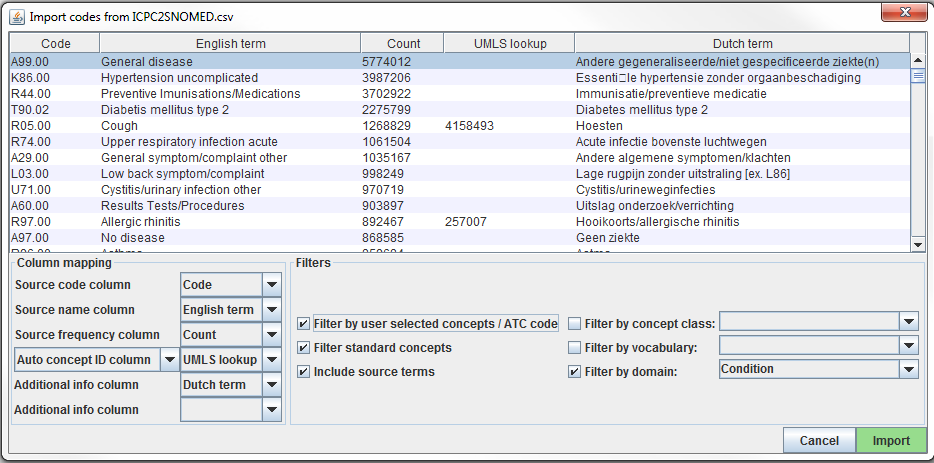
\includegraphics[width=1\linewidth]{images/ExtractTransformLoad/usagiImport} 

}

\caption{Usagi source code input screen.}\label{fig:usagiImport}
\end{figure}

The ``Column mapping'' section (bottom left) is where you define for
Usagi how to use the imported table. If you mouse hover over the drop
downs, a pop-up will appear defining each column. Usagi will not use the
``Additional info'' column(s) as information to associate source codes
to Vocabulary concept codes; however, this additional information may
help the individual reviewing the source code mapping and should be
included.

Finally, in the ``Filters'' section (bottom right) you can set some
restrictions for Usagi when mapping. For example, in Figure
\ref{fig:usagiImport}, the user is mapping the source codes only to
concepts in the Condition domain. By default, Usagi only maps to
Standard Concepts, but if the option ``Filter standard concepts'' is
turned off, Usagi will also consider Classification Concepts. Hover your
mouse over the different filters for additional information about the
filter.

One special filter is ``Filter by automatically selected concepts / ATC
code''. If there is information that you can use to restrict the search,
you can do so by providing a list of CONCEPT\_IDs or an ATC code in the
column indicated in the Auto concept ID column (semicolon-delimited).
For example, in the case of drugs there might already be ATC codes
assigned to each drug. Even though an ATC code does not uniquely
identify a single RxNorm drug code, it does help limit the search space
to only those concepts that fall under the ATC code in the Vocabulary.
To use the ATC code, follow these steps:

\begin{enumerate}
\def\labelenumi{\arabic{enumi}.}
\tightlist
\item
  In the Column mapping section, switch from ``Auto concept ID column''
  to ``ATC column''
\item
  In the Column mapping section, select the column containing the ATC
  code as ``ATC column''.
\item
  Turnon the ``Filter by user selected concepts / ATC code'' on in the
  Filters section.
\end{enumerate}

You can also use other sources of information than the ATC code to
restrict as well. In the example shown in the figure above, we used a
partial mapping derived from UMLS to restrict the Usagi search. In that
case we will need to use ``Auto concept ID column''.

Once all your settings are finalized, click the ``Import'' button to
import the file. The file import will take a few minutes as it is
running the term similarity algorithm to map source codes.

\subsubsection*{Reviewing Source Code to Vocabulary Concept
Maps}\label{reviewing-source-code-to-vocabulary-concept-maps}
\addcontentsline{toc}{subsubsection}{Reviewing Source Code to Vocabulary
Concept Maps}

Once you have imported your input file of source codes, the mapping
process begins. In Figure \ref{fig:usagiOverview}, you see the Usagi
screen is made up of 3 main sections: an overview table, the selected
mapping section, and place to perform searches. Note that in any of the
tables, you can right-click to select the columns that are shown or
hidden to reduce the visual complexity.

\begin{figure}

{\centering 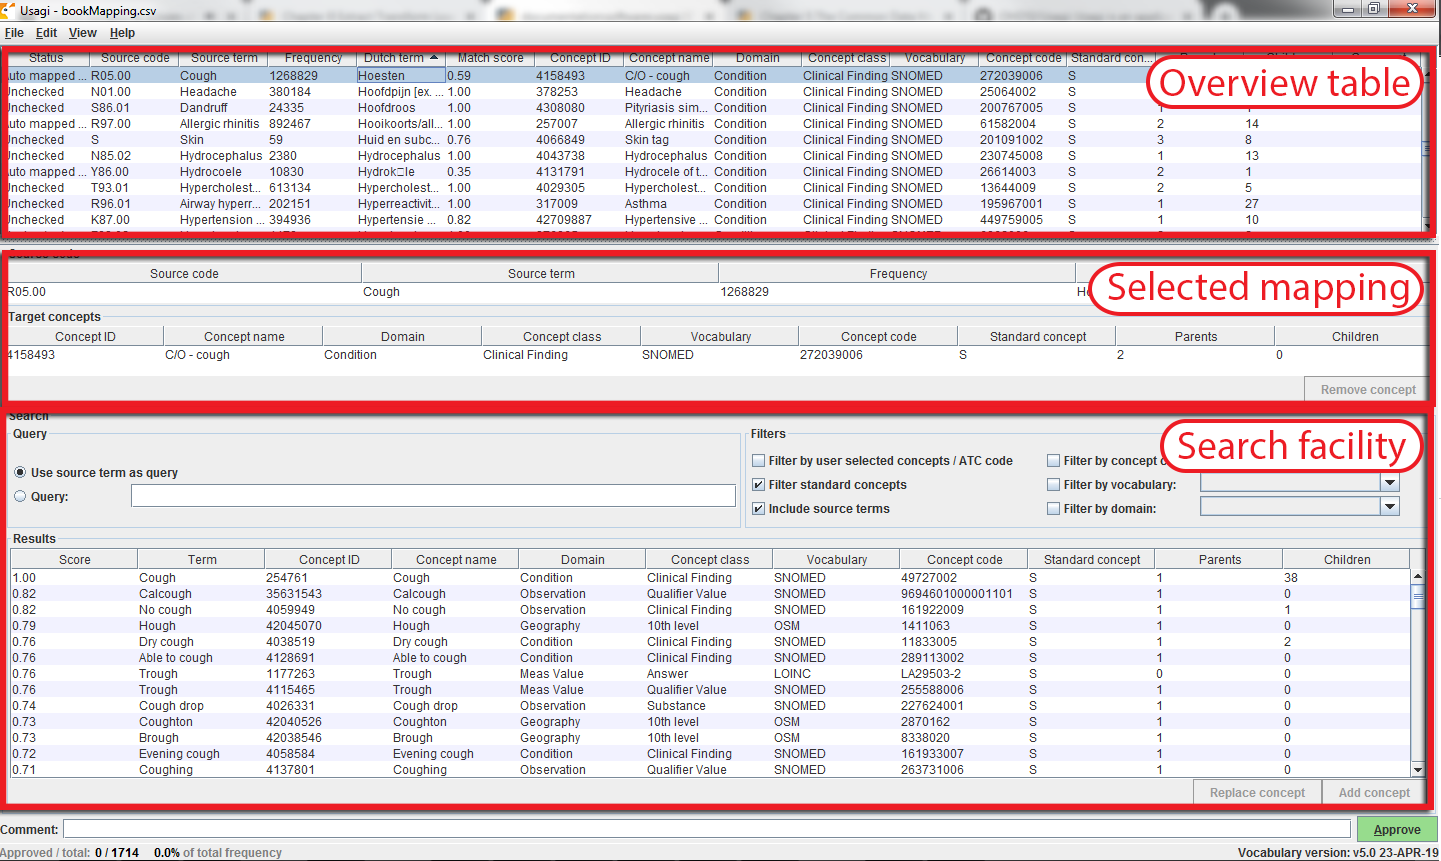
\includegraphics[width=1\linewidth]{images/ExtractTransformLoad/usagiOverview} 

}

\caption{Usagi source code input screen.}\label{fig:usagiOverview}
\end{figure}

\subsubsection*{Approving a Suggested
Mapping}\label{approving-a-suggested-mapping}
\addcontentsline{toc}{subsubsection}{Approving a Suggested Mapping}

The ``Overview Table'' shows the current mapping of source codes to
concepts. Right after importing source codes, this mapping contains the
automatically generated suggested mappings based on term similarity and
any search options. In the example in Figure \ref{fig:usagiOverview},
the English names of Dutch condition codes were mapped to standard
concepts in the Condition domain, because the user restricted the search
to that domain. Usagi compared the source code descriptions to concept
names and synonyms to find the best match. Because the user had selected
``Include source terms'' Usagi also considered the names and synonyms of
all source concepts in the vocabulary that map to a particular concept.
If Usagi is unable to make a mapping, it will map to the CONCEPT\_ID =
0.

It is suggested that someone with experience with coding systems help
map source codes to their associated standard vocabulary. That
individual will work through code by code in the ``Overview Table'' to
either accept the mapping Usagi has suggested or choose a new mapping.
For example in Figure \ref{fig:usagiOverview} we see that the Dutch term
``Hoesten'' which was translated to the English term ``Cough''. Usagi
used ``Cough'' and mapped it to the Vocabulary concept of ``4158493-C/O
- cough''. There was a matching score of 0.58 associated to this matched
pair (matching scores are typically 0 to 1 with 1 being a confident
match), a score of 0.58 signifies that Usagi is not very sure of how
well it has mapped this Dutch code to SNOMED. Let us say in this case,
we are okay with this mapping, we can approve it by hitting the green
``Approve'' button in the bottom right hand portion of the screen.

\subsubsection*{Searching for a New
Mapping}\label{searching-for-a-new-mapping}
\addcontentsline{toc}{subsubsection}{Searching for a New Mapping}

There will be cases where Usagi suggests a map and the user will be left
to either try to find a better mapping or set the map to no concept
(CONCEPT\_ID = 0). In the example given in Figure
\ref{fig:usagiOverview}, we see for the Dutch Term ``Hoesten'', which
was translated to ``Cough''. Usagi's suggestion was restricted by the
concept identified in our automatically derived mapping from UMLS, and
the result might not be optimal. In the Search Facility, we could search
for other concepts using either the actual term itself or a search box
query.

When using the manual search box, one should keep in mind that Usagi
uses a fuzzy search, and does not support structured search queries, so
for example not supporting Boolean operators like AND and OR.

To continue our example, suppose we used the search term ``Cough'' to
see if we could find a better mapping. On the right of the Query section
of the Search Facility, there is a Filters section, this provides
options to trim down the results from the Vocabulary when searching for
the search term. In this case we know we want to only find standard
concepts, and we allow concepts to be found based on the names and
synonyms of source concepts in the vocabulary that map to those standard
concepts.

When we apply these search criteria we find ``254761-Cough'' and feel
this may be an appropriate Vocabulary concept to map to our Dutch code.
In order to do that we can hit the ``Replace concept'' button, which you
will see in the ``Selected Source Code'' section update, followed by the
``Approve'' button. There is also an ``Add concept'' button, this allows
for multiple standardized Vocabulary concepts to map to one source code
(e.g.\,some source codes may bundle multiple diseases together while the
standardized vocabulary may not).

\subsubsection*{Concept Information}\label{concept-information}
\addcontentsline{toc}{subsubsection}{Concept Information}

When looking for appropriate concepts to map to, it is important to
consider the ``social life'' of a concept. The meaning of a concept
might depend partially on its place in the hierarchy, and sometimes
there are ``orphan concepts'' in the vocabulary with few or no
hierarchical relationships, which would be ill-suited as target
concepts. Usagi will often report the number of parents and children a
concept has, and it also possible to show more information by pressing
ALT + C or selecting view --\textgreater{} Concept information in the
top menu bar.

\begin{figure}

{\centering 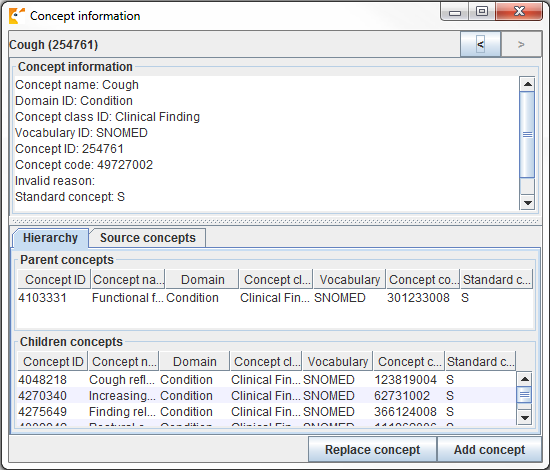
\includegraphics[width=1\linewidth]{images/ExtractTransformLoad/usagiConceptInfo} 

}

\caption{Usagi concept information panel.}\label{fig:usagiConceptInfo}
\end{figure}

Figure \ref{fig:usagiConceptInfo} shows the concept information panel.
It shows general information about a concept, as well as its parents,
children, and other source codes that map to the concept. Users can use
this panel to navigate the hierarchy and potentially choose a different
target concept.

Continue to move through this process, code by code, until all codes
have been checked. In the list of source codes at the top of the screen,
by selecting the column heading you can sort the codes. Often, we
suggest going from the highest frequency codes to the lowest. In the
bottom left of the screen you can see the number of codes that have
approved mappings, and how many code occurrences that corresponds to.

It is possible to add comments to mappings, which could be used to
document why a mapping decision was made.

\subsubsection*{Best Practices}\label{best-practices}
\addcontentsline{toc}{subsubsection}{Best Practices}

\begin{itemize}
\tightlist
\item
  Use someone who has experience with coding schemes.
\item
  By clicking on a column name, you can sort the columns in the
  ``Overview Table''. It may be valuable to sort on ``Match Score'';
  reviewing codes that Usagi is most confident on first may quickly
  knock out a significant chunk of codes. Also sorting on ``Frequency''
  is valuable, spending more effort on frequent codes versus
  non-frequent is important.
\item
  It is okay to map some codes to CONCEPT\_ID = 0, some codes may not be
  worth it to find a good map and others may just lack a proper map.
\item
  It is important to consider the context of a concept, specifically its
  parents and children.
\end{itemize}

\subsubsection*{Export the Usagi Map
Created}\label{export-the-usagi-map-created}
\addcontentsline{toc}{subsubsection}{Export the Usagi Map Created}

Once you have created your map within USAGI, the best way to use it
moving forward is to export it and append it to the Vocabulary
SOURCE\_TO\_CONCEPT\_MAP table.

To export your mappings, go to File --\textgreater{} Export
source\_to\_concept\_map. A pop-up will appear asking you which
SOURCE\_VOCABULARY\_ID you would like to use, type in a short
identifier. Usagi will use this identifier. as the
SOURCE\_VOCABULARY\_ID which will allow you to identify your specific
mapping in the SOURCE\_TO\_CONCEPT\_MAP table.

After selecting the SOURCE\_VOCABULARY\_ID, you give your export CSV a
name and save to location. The export CSV structure is in that of the
SOURCE\_TO\_CONCEPT\_MAP table. This mapping could be appended to the
Vocabulary's SOURCE\_TO\_CONCEPT\_MAP table. It would also make sense to
append a single row to the VOCABULARY table defining the
SOURCE\_VOCABULARY\_ID you defined in the step above. Finally, it is
important to note that only mappings with the ``Approved'' status will
be exported into the CSV file; the mapping needs to be completed in
USAGI in order to export it.

\subsubsection*{Updating an Usagi
Mapping}\label{updating-an-usagi-mapping}
\addcontentsline{toc}{subsubsection}{Updating an Usagi Mapping}

Often a mapping is not a one-time effort. As data is updated perhaps new
source codes are added, and the vocabulary is updated regularly, perhaps
requiring an update of the mapping.

When the set of source codes is updated the following steps can be
followed to support the update:

\begin{enumerate}
\def\labelenumi{\arabic{enumi}.}
\tightlist
\item
  Import the new source code file
\item
  Choose File --\textgreater{} Apply previous mapping, and select the
  old Usagi mapping file
\item
  Identify codes that haven't inherited approved mappings from the old
  mapping, and map them as usual.
\end{enumerate}

When the vocabulary is updated, follow these steps:

\begin{enumerate}
\def\labelenumi{\arabic{enumi}.}
\tightlist
\item
  Download the new vocabulary files from Athena
\item
  Rebuild the Usagi index (Help --\textgreater{} Rebuild index)
\item
  Open the mapping file
\item
  Identify codes that map to concepts that in the new vocabulary version
  no longer are Standard concepts, and find more appropriate target
  concepts.
\end{enumerate}

\section{Step 3: Implement the ETL}\label{step-3-implement-the-etl}

Once the design and code mappings are completed, the ETL process can be
implemented in a piece of software. When the ETL was being designed we
recommended that people who are knowledgeable about the source and CDM
work together on the task. Similarly, when the ETL is being implemented
it is preferred to use people who have experience with working with data
(particularly large data) and experience with implementing ETLs. This
may mean working with individuals outside of your immediate group or
hiring technical consultants to execute the implementation. It is also
important to note that this is not a one-time expense. Moving forward it
would be good to have someone or a team who spends at least some
dedicated time to maintaining and running the ETL (this will become
clearer in Section \ref{CDMandETLMaintenance}).

Implementation usually varies site to site and it largely depends on
many factors including infrastructure, size of the database, the
complexity of the ETL, and the technical expertise available. Because it
depends on many factors the OHDSI community does not make a formal
recommendation on how best to implement an ETL. There have been groups
that use simple SQL builders, SAS, C\#, Java, and Kettle. All have their
advantages and disadvantages, and none are usable if there is nobody at
the site who is familiar with the technology.

A few examples of different ETLs (listed in order of
complexity):\index{ETL!implementations}

\begin{itemize}
\tightlist
\item
  ETL-Synthea - A SQL builder written to convert the Synthea database
\item
  \url{https://github.com/OHDSI/etl-synthea}
\item
  ETL-CDMBuilder - A .NET application designed to transform multiple
  databases
\item
  \url{https://github.com/OHDSI/etl-cdmbuilder}
\item
  ETL-LambdaBuilder - A builder using the AWS lambda functionality
\item
  \url{https://github.com/OHDSI/etl-lambdabuilder}
\end{itemize}

It should be noted that after several independent attempts, we have
given up on developing the `ultimate' user-friendly ETL tool. It is
always the case that tools like that work well for 80\% of the ETL, but
for the remaining 20\% of the ETL some low-level code needs to be
written that is specific to a source database

Once the technical individuals are ready to start implementing, the ETL
design document should be shared with them. There should be enough
information in the documentation for them to get started however it
should be expected that the developers have access to the ETL designers
to ask questions during their development process. Logic that may be
clear to the designers may be less clear to an implementer who might not
be familiar with the data and CDM. The implementation phase should
remain a team effort. It is considered acceptable practice to go through
the process of CDM creation and testing between the implementers and
designers, respectively, until both groups are in agreement that all
logic has been executed correctly.

\section{Step 4: Quality Control}\label{step-4-quality-control}

For the extract, transform, load process, quality control is iterative.
The typical pattern is to write logic -\textgreater{} implement logic
-\textgreater{} test logic -\textgreater{} fix/write logic. There are
many ways to go about testing a CDM but below are recommend steps that
have been developed across the community through years of ETL
implementation. \index{ETL!quality control}

\begin{itemize}
\tightlist
\item
  Review of the ETL design document, computer code, and code mappings.
  Any one person can make mistakes, so always at least one other person
  should review what the what was done.
\item
  The largest issues in the computer code tend to come from how the
  source codes in the native data are mapped to Standard Concepts.
  Mapping can get tricky, especially when it comes to date-specific
  codes like NDCs. Be sure to double check any area where mappings are
  done to ensure the correct source vocabularies are translated to the
  proper concept id.\\
\item
  Manually compare all information on a sample of persons in the source
  and target data.
\item
  It can be helpful to walk through one person's data, ideally a person
  with a large number of unique records. Tracing through a single person
  can highlight issues if the data in the CDM is not how you expect it
  to look based on the agreed upon logic.
\item
  Compare overall counts in the source and target data.
\item
  There may be some expected differences in counts depending on how you
  chose to address certain issues. For instance, some collaborators
  choose to drop any people with a NULL gender since those people will
  not be included in analyses anyway. It may also be the case that
  visits in the CDM are constructed differently than visits or
  encounters in the native data. Therefore, when comparing overall
  counts between the source and CDM data be sure to account for and
  expect these differences.\\
\item
  Replicate a study that has already been performed on the source data
  on the CDM version.
\item
  This is a good way to understand any major differences between the
  source data and CDM version, though it is a little more
  time-intensive.
\item
  Create unit tests meant to replicate a pattern in the source data that
  should be addressed in the ETL. For example, if your ETL specifies
  that patients without gender information should be dropped, create a
  unit test of a person without a gender and assess how the builder
  handles it.
\item
  Unit testing is very handy when evaluating the quality and accuracy of
  an ETL conversion. It usually involves creating a much smaller dataset
  that mimics the structure of the source data you are converting. Each
  person or record in the dataset should test a specific piece of logic
  as written in the ETL document. Using this method, it is easy to trace
  back issues and to identify failing logic. The small size also enables
  the computer code to execute very quickly allowing for faster
  iterations and error identification.
\end{itemize}

These are high-level ways to approach quality control from an ETL
standpoint. For more detail on the data quality efforts going on within
OHDSI, please see Chapter \ref{DataQuality}.

\section{ETL Conventions and THEMIS}\label{etl-conventions-and-themis}

As more groups converted data to the CDM it became apparent that
conventions needed to be specified. For example, what should the ETL do
in a situation where a person record lacks a birth year? The goal of the
CDM is to standardized healthcare data however if every group handles
data specific scenarios differently it makes it more difficult to
systematically use data across the network.

The OHDSI community started documenting conventions to improve
consistency across CDMs. These defined conventions, that the OHDSI
community has agreed upon, can be found on the CDM Wiki.\footnote{\url{https://github.com/OHDSI/CommonDataModel/wiki}{]}.}
Each CDM table has its own set of conventions that can be referred to
when designing an ETL. For example, persons are allowed to be missing a
birth month or day, but if they lack a birth year the person should be
dropped. In designing an ETL, refer to the conventions to help make
certain design decisions that will be consistent with the community.

While it will never be possible to document all possible data scenarios
that exist and what to do when they occur, there is an OHDSI work group
trying to document common scenarios. THEMIS\footnote{\url{https://github.com/OHDSI/Themis}}
is made up of individuals in the community who gather conventions,
clarify them, share them with the community for comment, and then
document finalized conventions in the CDM Wiki. Themis is an ancient
Greek Titaness of divine order, fairness, law, natural law, and custom
which seemed a good fit for this groups remit. When performing an ETL,
if there is a scenario that you are unsure how to handle, THEMIS
recommends that a question about the scenario is posed on the OHDSI
Forums.\footnote{\url{http://forums.ohdsi.org/}} Most likely if you have
a question, others in the community probably have it as well. THEMIS
uses these discussions, as well as work group meetings and face-to-face
discussions, to help inform what other conventions need to be
documented.

\section{CDM and ETL Maintenance}\label{CDMandETLMaintenance}

It is no small effort to design the ETL, create the mappings, implement
the ETL, and build out quality control measures. Unfortunately, the
effort does not stop there. There is a cycle of ETL maintenance that is
a continuous process after the first CDM is built. Some common triggers
that require maintenance are: changes in the source data, a bug in the
ETL, a new OMOP Vocabulary is released, or the CDM itself has changed or
updated. If one of these triggers occur the following might need
updating: the ETL documentation, the software programming running the
ETL, and test cases and quality controls.

Often a healthcare data source is forever changing. New data might be
available (e.g.~a new column in the data might exist). Patience
scenarios that never existed before suddenly do (e.g.~a new patient who
has a death record before they were born). Your understanding of the
data may improve (e.g.~some of the records around inpatient child birth
come across as outpatient due to how claims are processed). Not all
changes in the source data my trigger a change in the ETL processing of
it, however at a bare minimum the changes that break the ETL processing
will need to be addressed.

If bugs are found, they should be addressed. However, it is important to
keep in mind that not all bugs are created equal. For example, let say
in the COST table the column cost was being rounded to a whole digit
(e.g.~the source data had \$3.82 and this became \$4.00 in the CDM). If
the primary researchers using the data were mostly performing
characterizations of patient's drug exposures and conditions, a bug such
as this is of little importance and can be addressed in the future. If
the primary researchers using the data also included health economists,
this would be a critical bug that need to be addressed immediately.

The OMOP Vocabulary is also ever changing just as our source data may
be. In fact, the Vocabulary can have multiple releases in one given
month as vocabularies update. Each CDM is run on a specific version of a
Vocabulary and running on a newer improved Vocabulary could result in
changes in how sources codes get mapped to in the standardized
vocabularies. Often differences between Vocabularies are minor, so
building a new CDM every time a new Vocabulary is release is not
necessary. However, it is good practice to adopt a new Vocabulary once
or twice a year which would require reprocessing the CDM again. It is
rare are there changes in a new version of a Vocabulary that would
require the ETL code itself to be updated.

The final trigger that could require CDM or ETL maintenance is when the
common data model itself updates. As the community grows and new data
requirements are found this may lead to additional data being stored in
the CDM. This might mean data that you previously were not storing in
the CDM might have a location in a new CDM version. Less frequently are
changes to existing CDM structure, however it is a possibility. For
example, the CDM is moved to adopting DATETIME fields over the original
DATE fields would could cause an error in ETL processing. CDM versions
are not released often and sites can choose when they migrate.

\section{Final Thoughts on ETL}\label{final-thoughts-on-etl}

The ETL process is a difficult one to master for many reasons, not the
least of which the fact that we are all working off unique source data,
making it hard to create a ``one-size-fits-all'' solution. However,
there are some hard won lessons we have learned over the years.

\begin{itemize}
\tightlist
\item
  The 80/20 rule. If you can avoid it do not spend too much time
  manually mapping source codes to concepts sets. Ideally, map the
  source codes that cover the majority of your data. This should be
  enough to get you started and you can address any remaining codes in
  the future based on use cases.
\item
  It's ok if you lose data that is not of research quality. Often these
  are the records that would be discarded before starting an analysis
  anyway, we just remove them during the ETL process instead.
\item
  A CDM requires maintenance. Just because you complete an ETL does not
  mean you do not need to touch it ever again. Your raw data might
  change, there might be a bug in the code, there may be new vocabulary
  or an update to the CDM. Plan for an allocate resources to these
  changes so your ETL is always up-to-date.
\item
  For support with getting started with the OHDSI CDM, performing your
  database conversion, or running the analytics tools, please visit our
  Implementers Forum.\footnote{\url{https://forums.ohdsi.org/c/implementers}}
\end{itemize}

\section{Summary}\label{summary-4}

\BeginKnitrBlock{rmdsummary}
\begin{itemize}
\item
  There is a generally agreed upon process for how to approach an ETL,
  including
\item
  Data experts and CDM experts together design the ETL
\item
  People with medical knowledge create the code mappings
\item
  A technical person implements the ETL
\item
  All are involved in quality control
\item
  Tools have been developed by the OHDSI community to facilitate these
  steps and are freely available for use
\item
  There are many ETL examples and agreed upon conventions you can use as
  a guide
\end{itemize}
\EndKnitrBlock{rmdsummary}

\section{Exercises}\label{exercises-2}

\BeginKnitrBlock{exercise}
\protect\hypertarget{exr:exerciseEtl1}{}{\label{exr:exerciseEtl1} }Put the
steps of the ETL process in the proper order:

\begin{enumerate}
\def\labelenumi{\Alph{enumi})}
\tightlist
\item
  Data experts and CDM experts together design the ETL
\item
  A technical person implements the ETL
\item
  People with medical knowledge create the code mappings
\item
  All are involved in quality control
\end{enumerate}
\EndKnitrBlock{exercise}

\BeginKnitrBlock{exercise}
\protect\hypertarget{exr:exerciseEtl2}{}{\label{exr:exerciseEtl2} }Using
OHDSI resources of your choice, spot four issues with the PERSON record
show in Table \ref{tab:exercisePersonTable} (table abbreviated for
space):

\begin{longtable}[]{@{}ll@{}}
\caption{\label{tab:exercisePersonTable} A PERSON table.}\tabularnewline
\toprule
Column & Value\tabularnewline
\midrule
\endfirsthead
\toprule
Column & Value\tabularnewline
\midrule
\endhead
PERSON\_ID & A123B456\tabularnewline
GENDER\_CONCEPT\_ID & 8532\tabularnewline
YEAR\_OF\_BIRTH & NULL\tabularnewline
MONTH\_OF\_BIRTH & NULL\tabularnewline
DAY\_OF\_BIRTH & NULL\tabularnewline
RACE\_CONCEPT\_ID & 0\tabularnewline
ETHNICITY\_CONCEPT\_ID & 8527\tabularnewline
PERSON\_SOURCE\_VALUE & A123B456\tabularnewline
GENDER\_SOURCE\_VALUE & F\tabularnewline
RACE\_SOURCE\_VALUE & WHITE\tabularnewline
ETHNICITY\_SOURCE\_VALUE & NONE PROVIDED\tabularnewline
\bottomrule
\end{longtable}
\EndKnitrBlock{exercise}

\BeginKnitrBlock{exercise}
\protect\hypertarget{exr:exerciseEtl3}{}{\label{exr:exerciseEtl3} }Let us
try to generate VISIT\_OCCURRENCE records. Here is some example logic
written for Synthea: Sort data in ascending order by PATIENT, START,
END. Then by PERSON\_ID, collapse lines of claim as long as the time
between the END of one line and the START of the next is \textless{}=1
day. Each consolidated inpatient claim is then considered as one
inpatient visit, set:

\begin{itemize}
\tightlist
\item
  MIN(START) as VISIT\_START\_DATE
\item
  MAX(END) as VISIT\_END\_DATE
\item
  ``IP'' as PLACE\_OF\_SERVICE\_SOURCE\_VALUE
\end{itemize}

If you see a set of visits as shown in Figure
\ref{fig:exerciseSourceData} in your source data, how would you expect
the resulting VISIT\_OCCURRENCE record(s) to look in the CDM?
\EndKnitrBlock{exercise}

\begin{figure}

{\centering 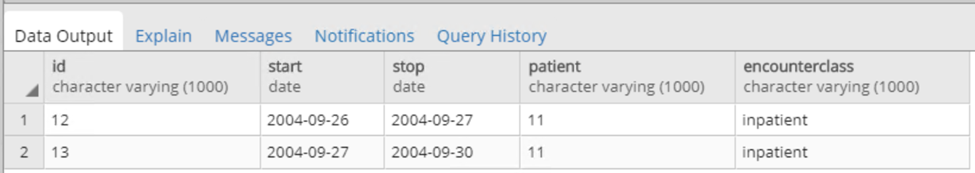
\includegraphics[width=1\linewidth]{images/ExtractTransformLoad/exerciseSourceData} 

}

\caption{Example source data.}\label{fig:exerciseSourceData}
\end{figure}

Suggested answers can be found in Appendix \ref{Etlanswers}.

\part{Data Analytics}\label{part-data-analytics}

\chapter{Data Analytics Use Cases}\label{DataAnalyticsUseCases}

\emph{Chapter lead: David Madigan}

The OHDSI collaboration focuses on generating reliable evidence from
real-world healthcare data, typically in the form of claims databases or
electronic health record databases. The use cases that OHDSI focuses on
fall into three major categories:

\begin{itemize}
\tightlist
\item
  Characterization
\item
  Population-level estimation
\item
  Patient-level prediction
\end{itemize}

We describe these in detail below. Note, for all the use cases, the
evidence we generate inherits the limitations of the data; we discuss
these limitations at length in the book section on Evidence Quality
(Chapters \ref{EvidenceQuality} - \ref{MethodValidity})

\section{Characterization}\label{characterization}

\index{characterization}

Characterization attempts to answer the question

\begin{quote}
What happened to them?
\end{quote}

We can use the data to provide answers to questions about the
characteristics of the persons in a cohort or the entire database, the
practice of healthcare, and study how these things change over time.

The data can provide answers to questions like:

\begin{itemize}
\tightlist
\item
  For patients newly diagnosed with atrial fibrillation, how many
  receive a prescription for warfarin?
\item
  What is the average age of patients who undergo hip arthroplasty?
\item
  What is the incidence rate of pneumonia in patients over 65 years old?
\end{itemize}

Typical characterization questions are formulated as:

\begin{itemize}
\tightlist
\item
  How many patients\ldots{}?
\item
  How often does\ldots{}?
\item
  What proportion of patients\ldots{}?
\item
  What is the distribution of values for lab\ldots{}?
\item
  What are the HbA1c levels for patients with\ldots{}?
\item
  What are the lab values for patients\ldots{}?
\item
  What is the median length of exposure for patients on\ldots{}.?
\item
  What are the trends over time in\ldots{}?
\item
  What are other drugs that these patients are using?
\item
  What are concomitant therapies?
\item
  Do we have enough cases of\ldots{}?
\item
  Would it be feasible to study X\ldots{}?
\item
  What are the demographics of\ldots{}?
\item
  What are the risk factors of\ldots{}? (if identifying a specific risk
  factor, maybe estimation, not prediction)
\item
  What are the predictors of\ldots{}?
\end{itemize}

And the desired output is:

\begin{itemize}
\tightlist
\item
  Count or percentage
\item
  Averages
\item
  Descriptive statistics
\item
  Incidence rate
\item
  Prevalence
\item
  Cohort
\item
  Rule-based phenotype
\item
  Drug utilization
\item
  Disease natural history
\item
  Adherence
\item
  Co-morbidity profile
\item
  Treatment pathways
\item
  Line of therapy
\end{itemize}

\section{Population-Level Estimation}\label{population-level-estimation}

\index{population-level estimation}

To a limited extent, the data can support causal inferences about the
effects of healthcare interventions, answering the question

\begin{quote}
What are the causal effects?
\end{quote}

We would like to understand causal effects to understand consequences of
actions. For example, if we decide to take some treatment, how does that
change what happens to us in the future?

The data can provide answers to questions like:

\begin{itemize}
\tightlist
\item
  For patients newly diagnosed with atrial fibrillation, in the first
  year after therapy initiation, does warfarin cause more major bleeds
  than dabigatran?
\item
  Does the causal effect of metformin on diarrhea vary by age?
\end{itemize}

Typical population-level effect estimation questions are formulated as:

\begin{itemize}
\tightlist
\item
  What is the effect of\ldots{}?
\item
  What if I do intervention\ldots{}?
\item
  Which treatment works better?
\item
  What is the risk of X on Y?
\item
  What is the time-to-event of\ldots{}?
\end{itemize}

And the desired output is:

\begin{itemize}
\tightlist
\item
  Relative risk
\item
  Hazards ratio
\item
  Odds ratio
\item
  Average treatment effect
\item
  Causal effect
\item
  Association
\item
  Correlation
\item
  Safety surveillance
\item
  Comparative effectiveness
\end{itemize}

\section{Patient-Level Prediction}\label{patient-level-prediction}

\index{patient-level prediction}

Based on the collected patient health histories in the database, we can
make patient-level predictions about future health events, answering the
question

\begin{quote}
What will happen to me?
\end{quote}

The data can provide answers to questions like:

\begin{itemize}
\tightlist
\item
  For a specific patient newly diagnosed with major depressive disorder,
  what is the probability the patient will attempt suicide in the first
  year following diagnosis?
\item
  For a specific patient newly diagnosed with atrial fibrillation, in
  the first year after therapy initiation with warfarin, what is the
  probability the patient suffers an ischemic stroke?
\end{itemize}

Typical patient-level prediction questions are formulated as:

\begin{itemize}
\tightlist
\item
  What is the chance that this patient will\ldots{}?
\item
  Who are candidates for\ldots{}?
\end{itemize}

And the desired output is:

\begin{itemize}
\tightlist
\item
  Probability for an individual
\item
  Prediction model
\item
  High/low risk groups
\item
  Probabilistic phenotype
\end{itemize}

Population-level estimation and patient-level prediction overlap to a
certain extent. For example, an important use case for prediction is to
predict an outcome for a specific patient had drug A been prescribed and
also predict the same outcome had drug B been prescribed. Let's assume
that in reality only one of these drugs is prescribed (say drug A) so we
get to see whether the outcome following treatment with A actually
occurs. Since drug B was not prescribed, the outcome following treatment
B, while predictable, is ``counterfactual'' since it is not ever
observed. Each of these prediction tasks falls under patient-level
prediction. However, the difference between (or ratio of) the two
outcomes is a unit-level \emph{causal} effect, and should be estimated
using causal effect estimation methods instead.

\BeginKnitrBlock{rmdimportant}
People have a natural tendency to erroneously interpret predictive
models as if they are causal models. But a predictive model can only
show correlation, never causation. For example, diabetic drug use might
be a strong predictor for myocardial infarction (MI) because diabetes is
a strong risk factor for MI. However, that does not mean that stopping
the diabetic drugs will prevent MI!
\EndKnitrBlock{rmdimportant}

\section{Example Use Cases in
Hypertension}\label{example-use-cases-in-hypertension}

You're a researcher interested in studying the effects of ACE inhibitor
monotherapy vs.~thiazide diuretic monotherapy on the outcomes of acute
myocardial infarction and angioedema as first-line treatment for
hypertension. You understand that based on the OHDSI literature, you are
asking a population-level effect estimation question but first, you need
to do some homework on how to characterize this particular treatment of
interest.

\subsection{Characterization
Questions}\label{characterization-questions}

Acute myocardial infarction is a cardiovascular complication that can
occur in patients with high blood pressure, so effective treatment for
hypertension should reduce the risk. Angioedema is a known side effect
of ACE inhibitors, which is rare but potentially serious. You start by
creating cohorts (see Chapter \ref{Cohorts}) for the exposures of
interest (new users of ACE inhibitors and new users of thiazide
diuretics). You perform a characterization (see Chapter
\ref{Characterization}) analysis to summarize baseline characteristics
of these exposure populations, including demographics, co morbid
conditions, and concomitant medications. You perform another
characterization analysis to estimate the incidence of selected outcomes
within these exposure populations. Here, you ask `how often does 1)
acute myocardial infarction and 2) angioedema occur during the period of
exposure to ACE inhibitors and thiazide diuretics?' These
characterizations allow us to assess the feasibility of conducting a
population-level estimation study, to evaluate whether the two treatment
groups are comparable, and to identify `risk factors' that might predict
which treatment choice that patients made.

\subsection{Population-Level Estimation
Question}\label{population-level-estimation-question}

The population-level effect estimation study (see Chapter
\ref{PopulationLevelEstimation}) estimates the relative risk of ACE
inhibitor vs, thiazide use for the outcomes of AMI and angioedema. Here,
you further evaluate through study diagnostics and negative controls
whether we can produce a reliable estimate of the average treatment
effect.

\subsection{Patient-Level Prediction
Question}\label{patient-level-prediction-question}

Independent of whether there is a causal effect of the exposures, you
are also interested in trying to determine which patients are at highest
risk of the outcomes. This is a patient-level prediction problem (see
Chapter \ref{PatientLevelPrediction}). Here, you develop a prediction
model that evaluates: amongst the patients who are new users of ACE
inhibitors, which patients are at highest risk of developing acute
myocardial infarction during the 1 year after starting treatment. The
model allows us to predict, for a patient who has just been prescribed
ACE for the first time, based on events observed from their medical
history, what is the chance that they will experience AMI in the next 1
year.

\section{Limitations of Observational
Research}\label{limitations-of-observational-research}

\index{limitations of obervational research}

There are many important healthcare questions for which OHDSI databases
cannot provide answers. These include:

\begin{itemize}
\tightlist
\item
  Causal effects of interventions compared to placebo. Sometimes it is
  possible to consider the causal effect of a treatment as compared with
  non-treatment but not placebo treatment.
\item
  Anything related to over-the-counter medications.
\item
  Many outcomes and other variables are sparsely recorded if at all.
  These include mortality, behavioral outcomes, lifestyle, and
  socioeconomic status.
\item
  Since patients tend to encounter the healthcare system only when they
  are unwell, measurement of the benefits of treatments can prove
  elusive.
\end{itemize}

\subsection{Erroneous Data}\label{erroneous-data}

Clinical data recorded in OHDSI databases can deviate from clinical
reality. For example, a patient's record may include a code for
myocardial infarction even though the patient never experienced a
myocardial infarction. Similarly, a lab value may be erroneous or an
incorrect code for a procedure may appear in the database. Chapters
\ref{DataQuality} and \ref{ClinicalValidity} discuss several of these
issues and good practice aims to identify and correct for as many of
these kinds of issues as possible. Nonetheless, erroneous data
inevitably persist to some extent and can undermine the validity of
subsequent analyses. An extensive literature focuses on adjustment of
statistical inferences to account for errors-in-data - see, for example,
\citet{fuller2009measurement}.

\subsection{Missing Data}\label{missing-data}

\index{missing data}

Missingness in OHDSI databases presents subtle challenges. A health
event (e.g., prescription, laboratory value, etc.) that should be
recorded in a database, but isn't, is ``missing.'' The statistics
literature distinguishes between types of missingness such as ``missing
completely at random,'' ``missing at random,'' and ``missing not at
random'' and methods of increasing complexity attempt to address these
types. \citet{perkins2017principled} provide a useful introduction to
this topic.

\section{Summary}\label{summary-5}

\BeginKnitrBlock{rmdsummary}
\begin{itemize}
\item
  In observational research we distinguish three large categories of
  uses cases.
\item
  \textbf{Characterization} aims to answer the questions ``What happened
  to them?''
\item
  \textbf{Population-level estimation} attempts to answer the question
  ``What are the causal effects?''
\item
  \textbf{Patient-level prediction} tries to answer ``What will happen
  to me?''
\item
  Prediction models are not causal models; There is no reason to believe
  that intervening on a strong predictor will impact the outcome.
\item
  There are questions that cannot be answered using observational
  healthcare data.
\end{itemize}
\EndKnitrBlock{rmdsummary}

\section{Exercises}\label{exercises-3}

\BeginKnitrBlock{exercise}
\protect\hypertarget{exr:exerciseUseCases1}{}{\label{exr:exerciseUseCases1}
}Which use case categories do these questions belong to?

\begin{enumerate}
\def\labelenumi{\arabic{enumi}.}
\item
  Compute the rate of gastrointestinal (GI) bleeding in patients
  recently exposed to NSAIDs.
\item
  Compute the probability that a specific patient experiences a GI bleed
  in the next year, based on their baseline characteristics.
\item
  Estimate the increased risk of GI bleeding due to diclofenac compared
  to celecoxib.
\end{enumerate}
\EndKnitrBlock{exercise}

\BeginKnitrBlock{exercise}
\protect\hypertarget{exr:exerciseUseCases2}{}{\label{exr:exerciseUseCases2}
}You wish to estimate the increased risk of GI bleeding due to
diclofenac compared to no exposure (placebo). Can this be done using
observational healthcare data?
\EndKnitrBlock{exercise}

Suggested answers can be found in Appendix \ref{UseCasesanswers}.

\chapter{OHDSI Analytics Tools}\label{OhdsiAnalyticsTools}

\emph{Chapter leads: Martijn Schuemie \& Frank DeFalco}

OHDSI offers a wide range of open source tools to support various
data-analytics use cases on observational patient-level data. What these
tools have in common is that they can all interact with one or more
databases using the Common Data Model (CDM). Furthermore, these tools
standardize the analytics for various use cases; Rather than having to
start from scratch, an analysis can be implemented by filling in
standard templates. This makes performing analysis easier, and also
improves reproducibility and transparency. For example, there appear to
be a near-infinite number of ways to compute an incidence rate, but
these can be specified in the OHDSI tools with a few choices, and anyone
making those same choices will compute incidence rates the same way.

In this chapter we first describe various ways in which we can choose to
implement an analysis, and what strategies the analysis can employ. We
then review the various OHDSI tools and how they fit the various use
cases.

\section{Analysis Implementation}\label{analysisImplementation}

Figure \ref{fig:implementations} shows the various ways in which we can
choose to implement a study against a database using the CDM.
\index{analysis implementation}

\begin{figure}

{\centering 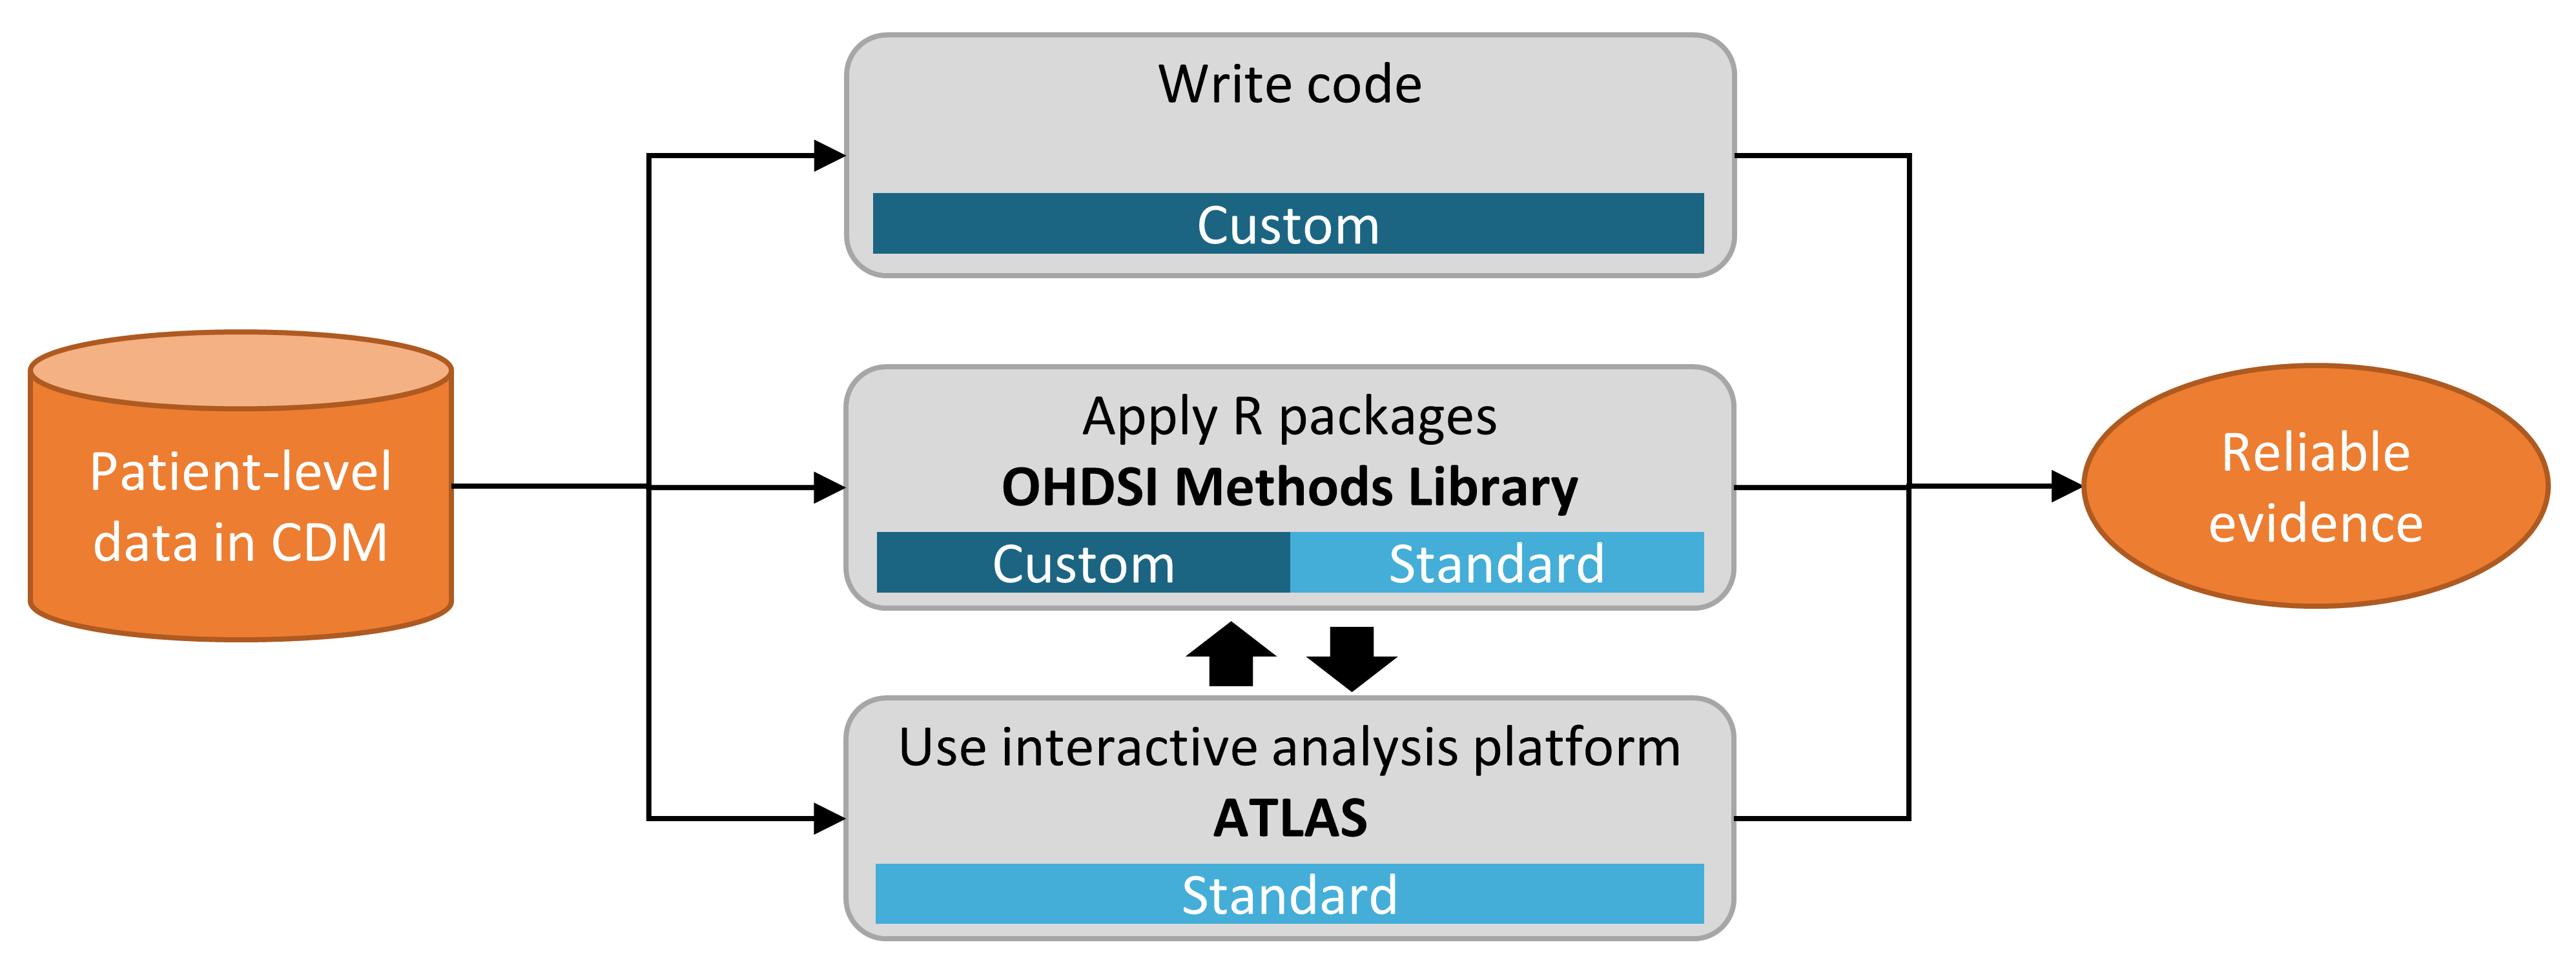
\includegraphics[width=0.9\linewidth]{images/OhdsiAnalyticsTools/implementations} 

}

\caption{Different ways to implement an analysis against data in the CDM.}\label{fig:implementations}
\end{figure}

There are three main approaches to implementing a study. The first is to
write custom code that does not make use of any of the tools OHDSI has
to offer. One could write a de novo analysis in R, SAS, or any other
language. This provides the maximum flexibility, and may in fact be the
only option if the specific analysis is not supported by any of our
tools. However, this path requires a lot of technical skill, time, and
effort, and as the analysis increases in complexity it becomes harder to
avoid errors in the code.

The second approach involves developing the analysis in R, and making
use of the packages in the
\href{https://ohdsi.github.io/MethodsLibrary/}{OHDSI Methods Library}.
At a minimum, one could use the
\href{https://ohdsi.github.io/SqlRender/}{SqlRender} and
\href{https://ohdsi.github.io/DatabaseConnector/}{DatabaseConnector}
packages described in more detail in Chapter \ref{SqlAndR} that allow
the same code to be executed on various database platforms, such as
PostgreSQL, SQL Server, and Oracle. Other packages such as
\href{https://ohdsi.github.io/CohortMethod/}{CohortMethod} and
\href{https://ohdsi.github.io/PatientLevelPrediction/}{PatientLevelPrediction}
offer R functions for advanced analytics against the CDM that can be
called on in one's code. This still requires a lot of technical
expertise, but by re-using the validated components of the Methods
Library we can be more efficient and less prone to error than when using
completely custom code.

The third approach relies on our interactive analysis platform
\href{https://github.com/OHDSI/Atlas/wiki}{ATLAS}, a web-based tool that
allows non-programmers to perform a wide range of analyses efficiently.
ATLAS makes use of the Methods Libraries but provides a simple graphical
interface to design analyses and in many cases generate the necessary R
code to run the analysis. However, ATLAS does not support all options
available in the Methods Library. While it is expected that the majority
of studies can be performed through ATLAS, some studies may require the
flexibility offered by the second approach.

ATLAS and the Methods Library are not independent. Some of the more
complicated analytics that can be invoked in ATLAS are executed through
calls to the packages in the Methods Library. Similarly, cohorts used in
the Methods Library are often designed in ATLAS.

\section{Analysis Strategies}\label{analysis-strategies}

In addition to the strategy used to implement our analysis against the
CDM, for example through custom coding or use of standard analytic code
in the Methods Library, there are also multiple strategies for using
those analytic techniques to generate evidence. Figure
\ref{fig:strategies} highlights three strategies that are employed in
OHDSI.

\begin{figure}

{\centering 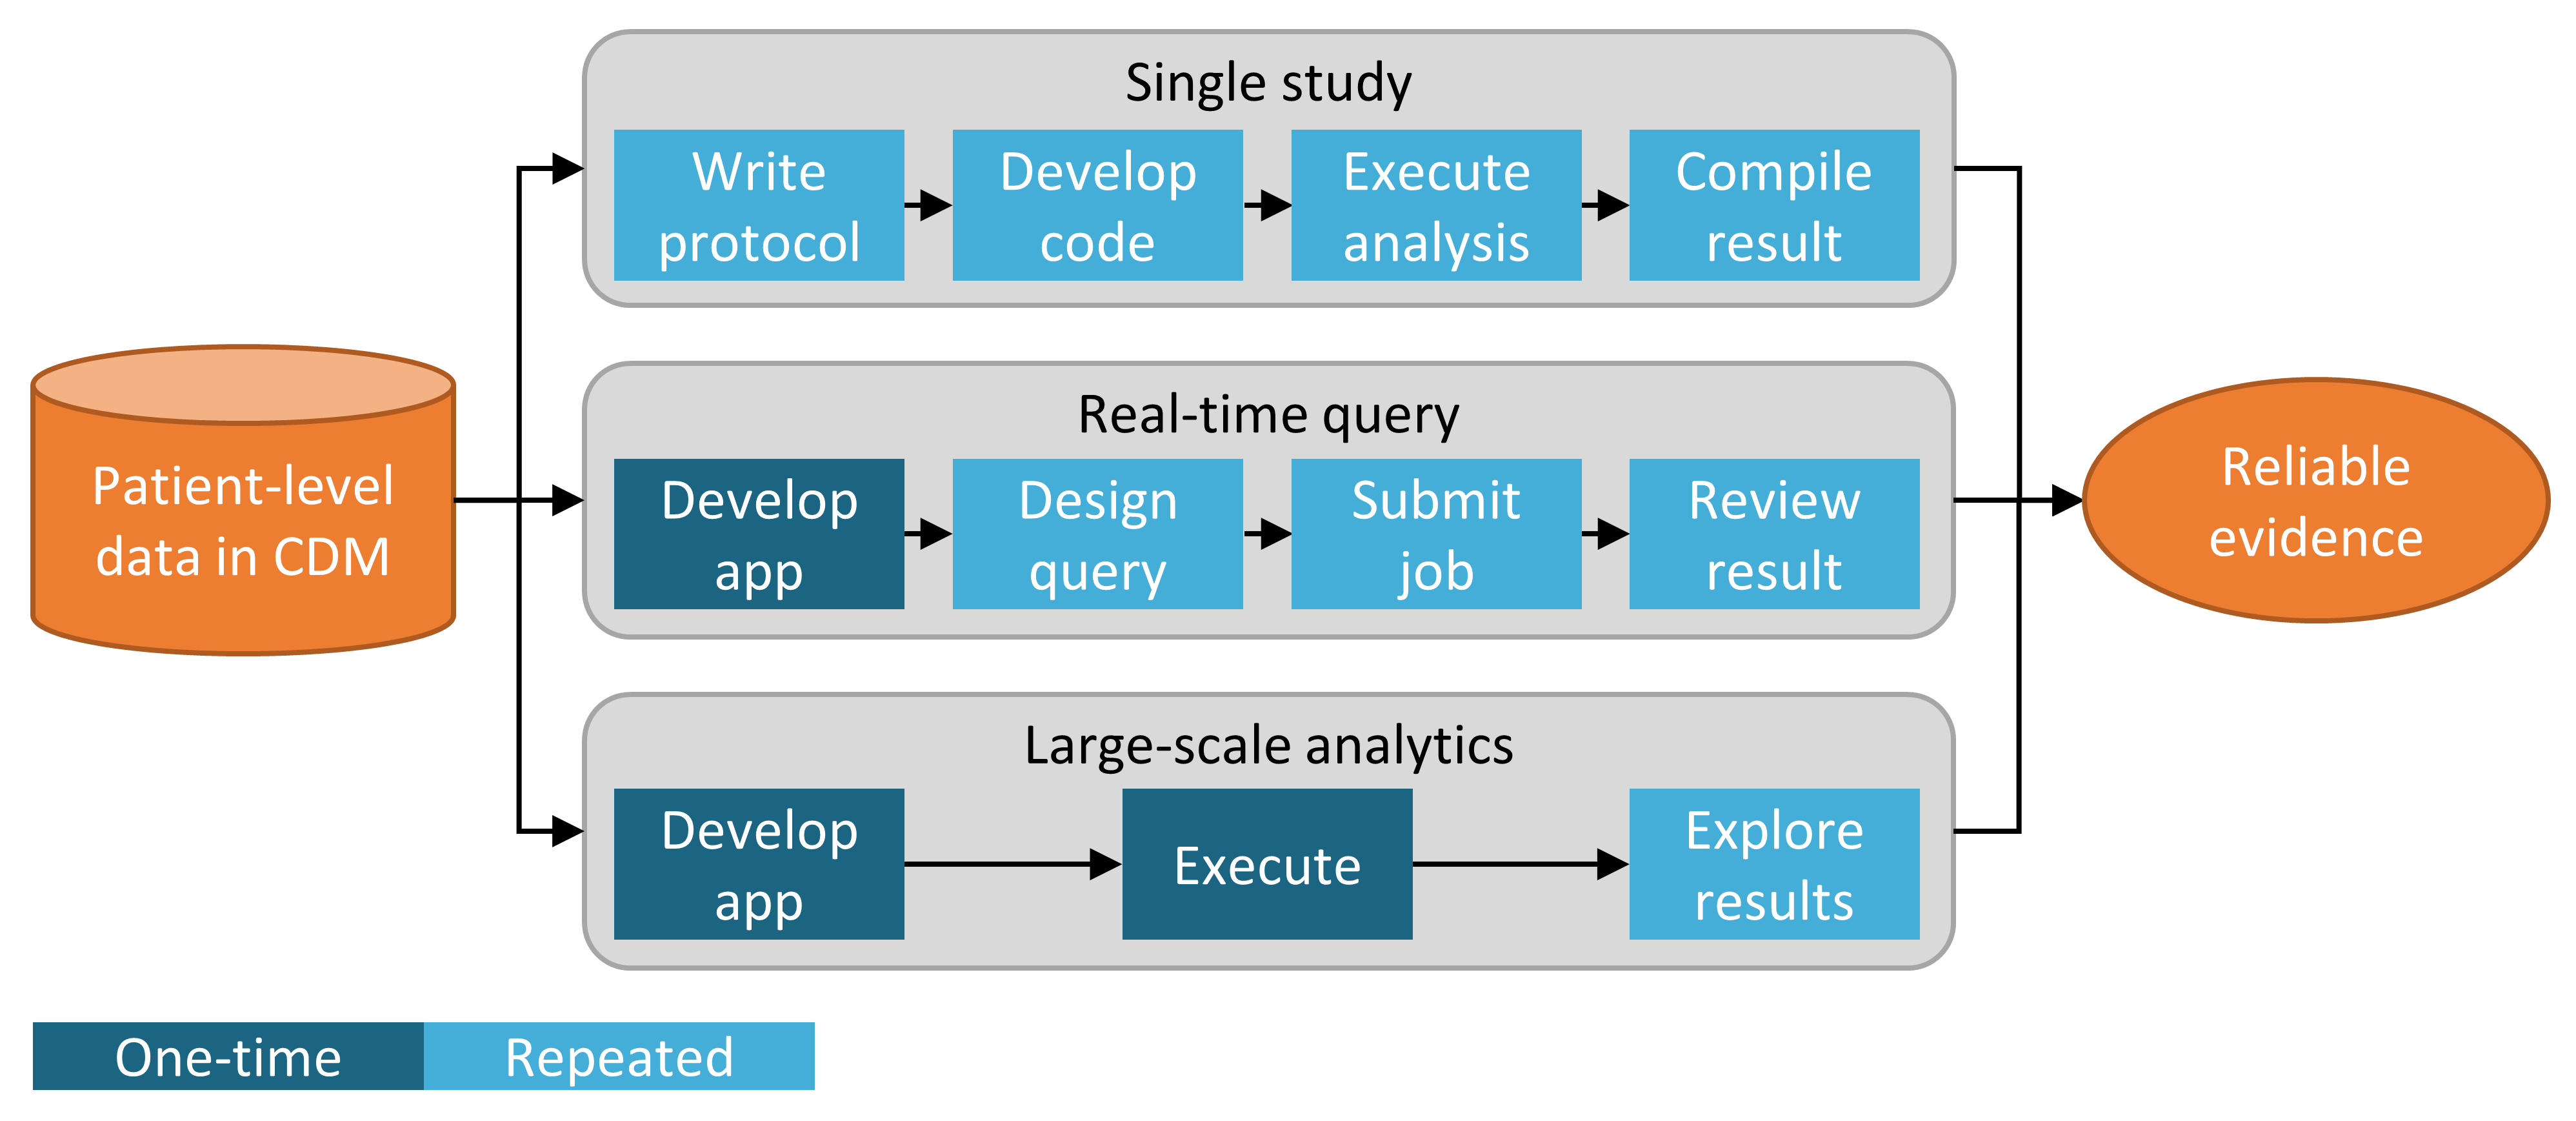
\includegraphics[width=0.9\linewidth]{images/OhdsiAnalyticsTools/strategies} 

}

\caption{Strategies for generating evidence for (clinical) questions.}\label{fig:strategies}
\end{figure}

The first strategy views every analysis as a single individual study.
The analysis must be pre-specified in a protocol, implemented as code,
executed against the data, after which the result can be compiled and
interpreted. For every question, all steps must be repeated. An example
of such an analysis is the OHDSI study into the risk of angioedema
associated with levetiracetam compared with phenytoin. \citep{duke_2017}
Here, a protocol was first written, analysis code using the OHDSI
Methods Library was developed and executed across the OHDSI network, and
results were compiled and disseminated in a journal publication.

The second strategy develops an application that allows users to answer
a specific class of questions in real time or near-real time. Once the
application has been developed, users can interactively define queries,
submit them, and view the results. An example of this strategy is the
cohort definition and generation tool in ATLAS. This tool allows users
to specify cohort definitions of varying complexity, and execute the
definition against a database to see how many people meet the various
inclusion and exclusion criteria.

The third strategy similarly focuses on a class of questions, but then
attempts to exhaustively generate all the evidence for the questions
within the class. Users can then explore the evidence as needed through
a variety of interfaces. One example is the OHDSI study into the effects
of depression treatments. \citep{schuemie_2018b} In this study all
depression treatments are compared for a large set of outcomes of
interest across four large observational databases. The full set of
results, including 17,718 empirically calibrated hazard ratios along
with extensive study diagnostics, is available in an interactive web
app.\footnote{\url{http://data.ohdsi.org/SystematicEvidence/}}

\section{ATLAS}\label{atlas}

ATLAS is a free, publicly available, web-based tool developed by the
OHDSI community that facilitates the design and execution of analyses on
standardized, patient-level, observational data in the CDM format. ATLAS
is deployed as a web application in combination with the OHDSI WebAPI
and is typically hosted on Apache Tomcat. Performing real time analyses
requires access to the patient-level data in the CDM and is therefore
typically installed behind an organization's firewall. However, there is
also a public ATLAS\footnote{\url{http://www.ohdsi.org/web/atlas}}, and
although this ATLAS instance only has access to a few small simulated
datasets, it can still be used for many purposes including testing and
training. It is even possible to fully define an effect estimation or
prediction study using the public instance of ATLAS, and automatically
generate the R code for executing the study. That code can then be run
in any environment with an available CDM without needing to install
ATLAS and the WebAPI. \index{ATLAS}

\begin{figure}

{\centering 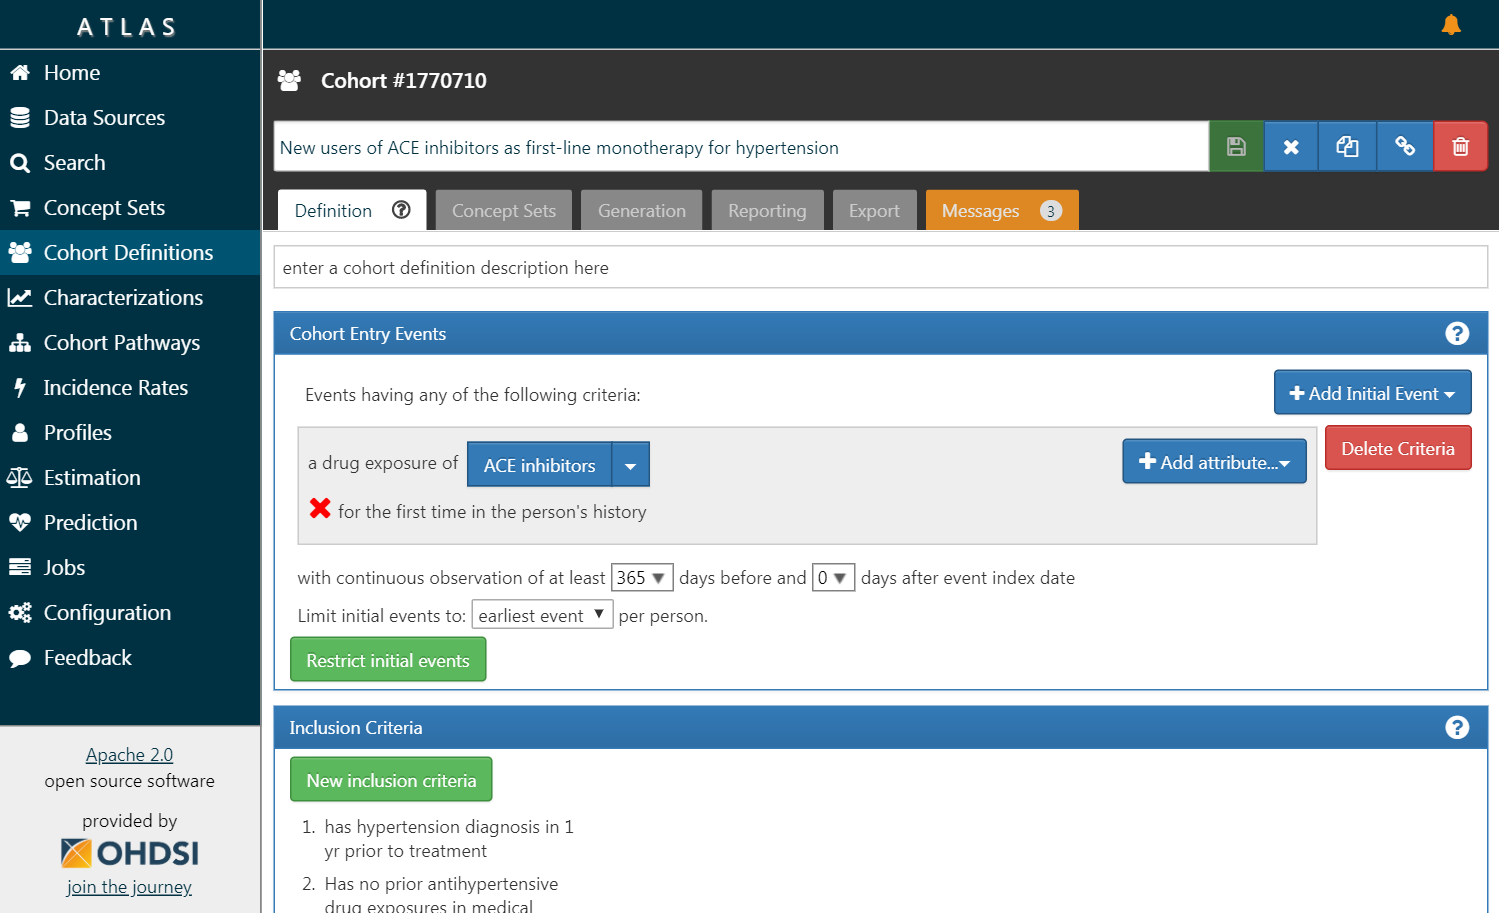
\includegraphics[width=1\linewidth]{images/OhdsiAnalyticsTools/atlas} 

}

\caption{ATLAS user interface.}\label{fig:atlas}
\end{figure}

A screenshot of ATLAS is provided in Figure \ref{fig:atlas}. On the left
is a navigation bar showing the various functions provided by ATLAS:

\begin{description}
\tightlist
\item[Data Sources \index{ATLAS!Data Sources}
\index{Achilles|see {ATLAS!data sources}}]
Data sources provides the capability review descriptive, standardized
reporting for each of the data sources that you have configured within
your Atlas platform. This feature uses the large-scale analytics
strategy: all descriptives have been pre-computed. Data sources is
discussed in Chapter \ref{Characterization}.
\item[Vocabulary Search \index{ATLAS!vocabulary search}]
Atlas provides the ability to search and explore the OMOP standardized
vocabulary to understand what concepts exist within those vocabularies
and how to apply those concepts in your standardized analysis against
your data sources. This feature is discussed in Chapter
\ref{StandardizedVocabularies}.
\item[Concept Sets \index{ATLAS!concept sets}]
Concept sets provides the ability to create collections of logical
expressions that can be used to identify a set of concepts to be used
throughout your standardized analyses. Concept sets provide more
sophistication than a simple list of codes or values. A concept set is
comprised of multiple concepts from the standardized vocabulary in
combination with logical indicators that allow a user to specify that
they are interested in including or excluding related concepts in the
vocabulary hierarchy. Searching the vocabulary, identifying the set of
concepts, and specifying the logic to be used to resolve a concept set
provides a powerful mechanism for defining the often obscure medical
language used in analysis plans. These concept sets can be saved within
ATLAS and then used throughout your analysis as part of cohort
definitions or analysis specifications.
\item[Cohort Definitions \index{ATLAS!cohort definitions}]
Cohort definitions is the ability to construct a set of persons who
satisfy one or more criteria for a duration of time and these cohorts
can then serve as the basis of inputs for all of your subsequent
analyses. This feature is discussed in Chapter \ref{Cohorts}.
\item[Characterizations \index{ATLAS!cohort characterization}]
Characterizations is an analytic capability that allows you to look at
one or more cohorts that you've defined and to summarize characteristics
about those patient populations. This feature uses the real-time query
strategy, and is discussed in Chapter \ref{Characterization}.
\item[Cohort Pathways \index{ATLAS!cohort pathways}]
Cohort pathways is an analytic tool that allows you to look at the
sequence of clinical events that occur within one or more populations.
This feature uses the real-time query strategy, and is discussed in
Chapter \ref{Characterization}.
\item[Incidence Rates \index{ATLAS!incidence rates}]
Incidence rates is a tool that allows you to estimate the incidence of
outcomes within target populations of interest. This feature uses the
real-time query strategy, and is discussed in Chapter
\ref{Characterization}.
\item[Profiles \index{ATLAS!profiles}]
Profiles is a tool that allows you to explore an individual patients
longitudinal observational data to summarize what is going on within a
given individual. This feature uses the real-time query strategy.
\item[Population Level Estimation
\index{ATLAS!population level estimation}]
Estimation is a capability to allow you to define a population level
effect estimation study using a comparative cohort design whereby
comparisons between one or more target and comparator cohorts can be
explored for a series of outcomes. This feature can be said to implement
the real-time query strategy, as no coding is required, and is discussed
in Chapter \ref{PopulationLevelEstimation}.
\item[Patient Level Prediction \index{ATLAS!patient level prediction}]
Prediction is a capability to allow you to apply machine learning
algorithms to conduct patient level prediction analyses whereby you can
predict an outcome within any given target exposures. This feature can
be said to implement the real-time query strategy, as no coding is
required, and is discussed in Chapter \ref{PatientLevelPrediction}.
\item[Jobs \index{ATLAS!jobs}]
Select the Jobs menu item to explore the state of processes that are
running through the WebAPI. Jobs are often long running processes such
as generating a cohort or computing cohort characterization reports.
\item[Configuration \index{ATLAS!configuration}]
Select the Configuration menu item to review the data sources that have
been configured in the source configuration section.
\item[Feedback \index{ATLAS!feedback}]
The Feedback link will take you to the issue log for Atlas so that you
can log a new issue or to search through existing issues. If you have
ideas for new features or enhancements, this is also a place note these
for the development community.
\end{description}

\subsection{Security}\label{security}

ATLAS and the WebAPI provide a granular security model to control access
to features or data sources within the overall platform. The security
system is built leveraging the Apache Shiro library. Additional
information on the security system can be found in the online WebAPI
security wiki.\footnote{\url{https://github.com/OHDSI/WebAPI/wiki/Security-Configuration}}
\index{ATLAS!security}

\subsection{Documentation}\label{documentation}

Documentation for ATLAS can be found online in the ATLAS GitHub
repository wiki.\footnote{\url{https://github.com/OHDSI/ATLAS/wiki}}
This wiki includes information on the various application features as
well as links to online video tutorials. \index{ATLAS!documentation}

\subsection{How to Install}\label{how-to-install}

Installation of ATLAS is done in combination with the OHDSI WebAPI.
Installation guides for each component are available online in the ATLAS
GitHub repository Setup Guide\footnote{\url{https://github.com/OHDSI/Atlas/wiki/Atlas-Setup-Guide}}
and WebAPI GitHub repository Installation Guide.\footnote{\url{https://github.com/OHDSI/WebAPI/wiki/WebAPI-Installation-Guide}}
\index{ATLAS!installation}

\section{Methods Library}\label{methods-library}

The \href{https://ohdsi.github.io/MethodsLibrary/}{OHDSI Methods
Library} is the collection of open source R packages show in Figure
\ref{fig:methodsLibrary}. \index{methods library}

\begin{figure}

{\centering 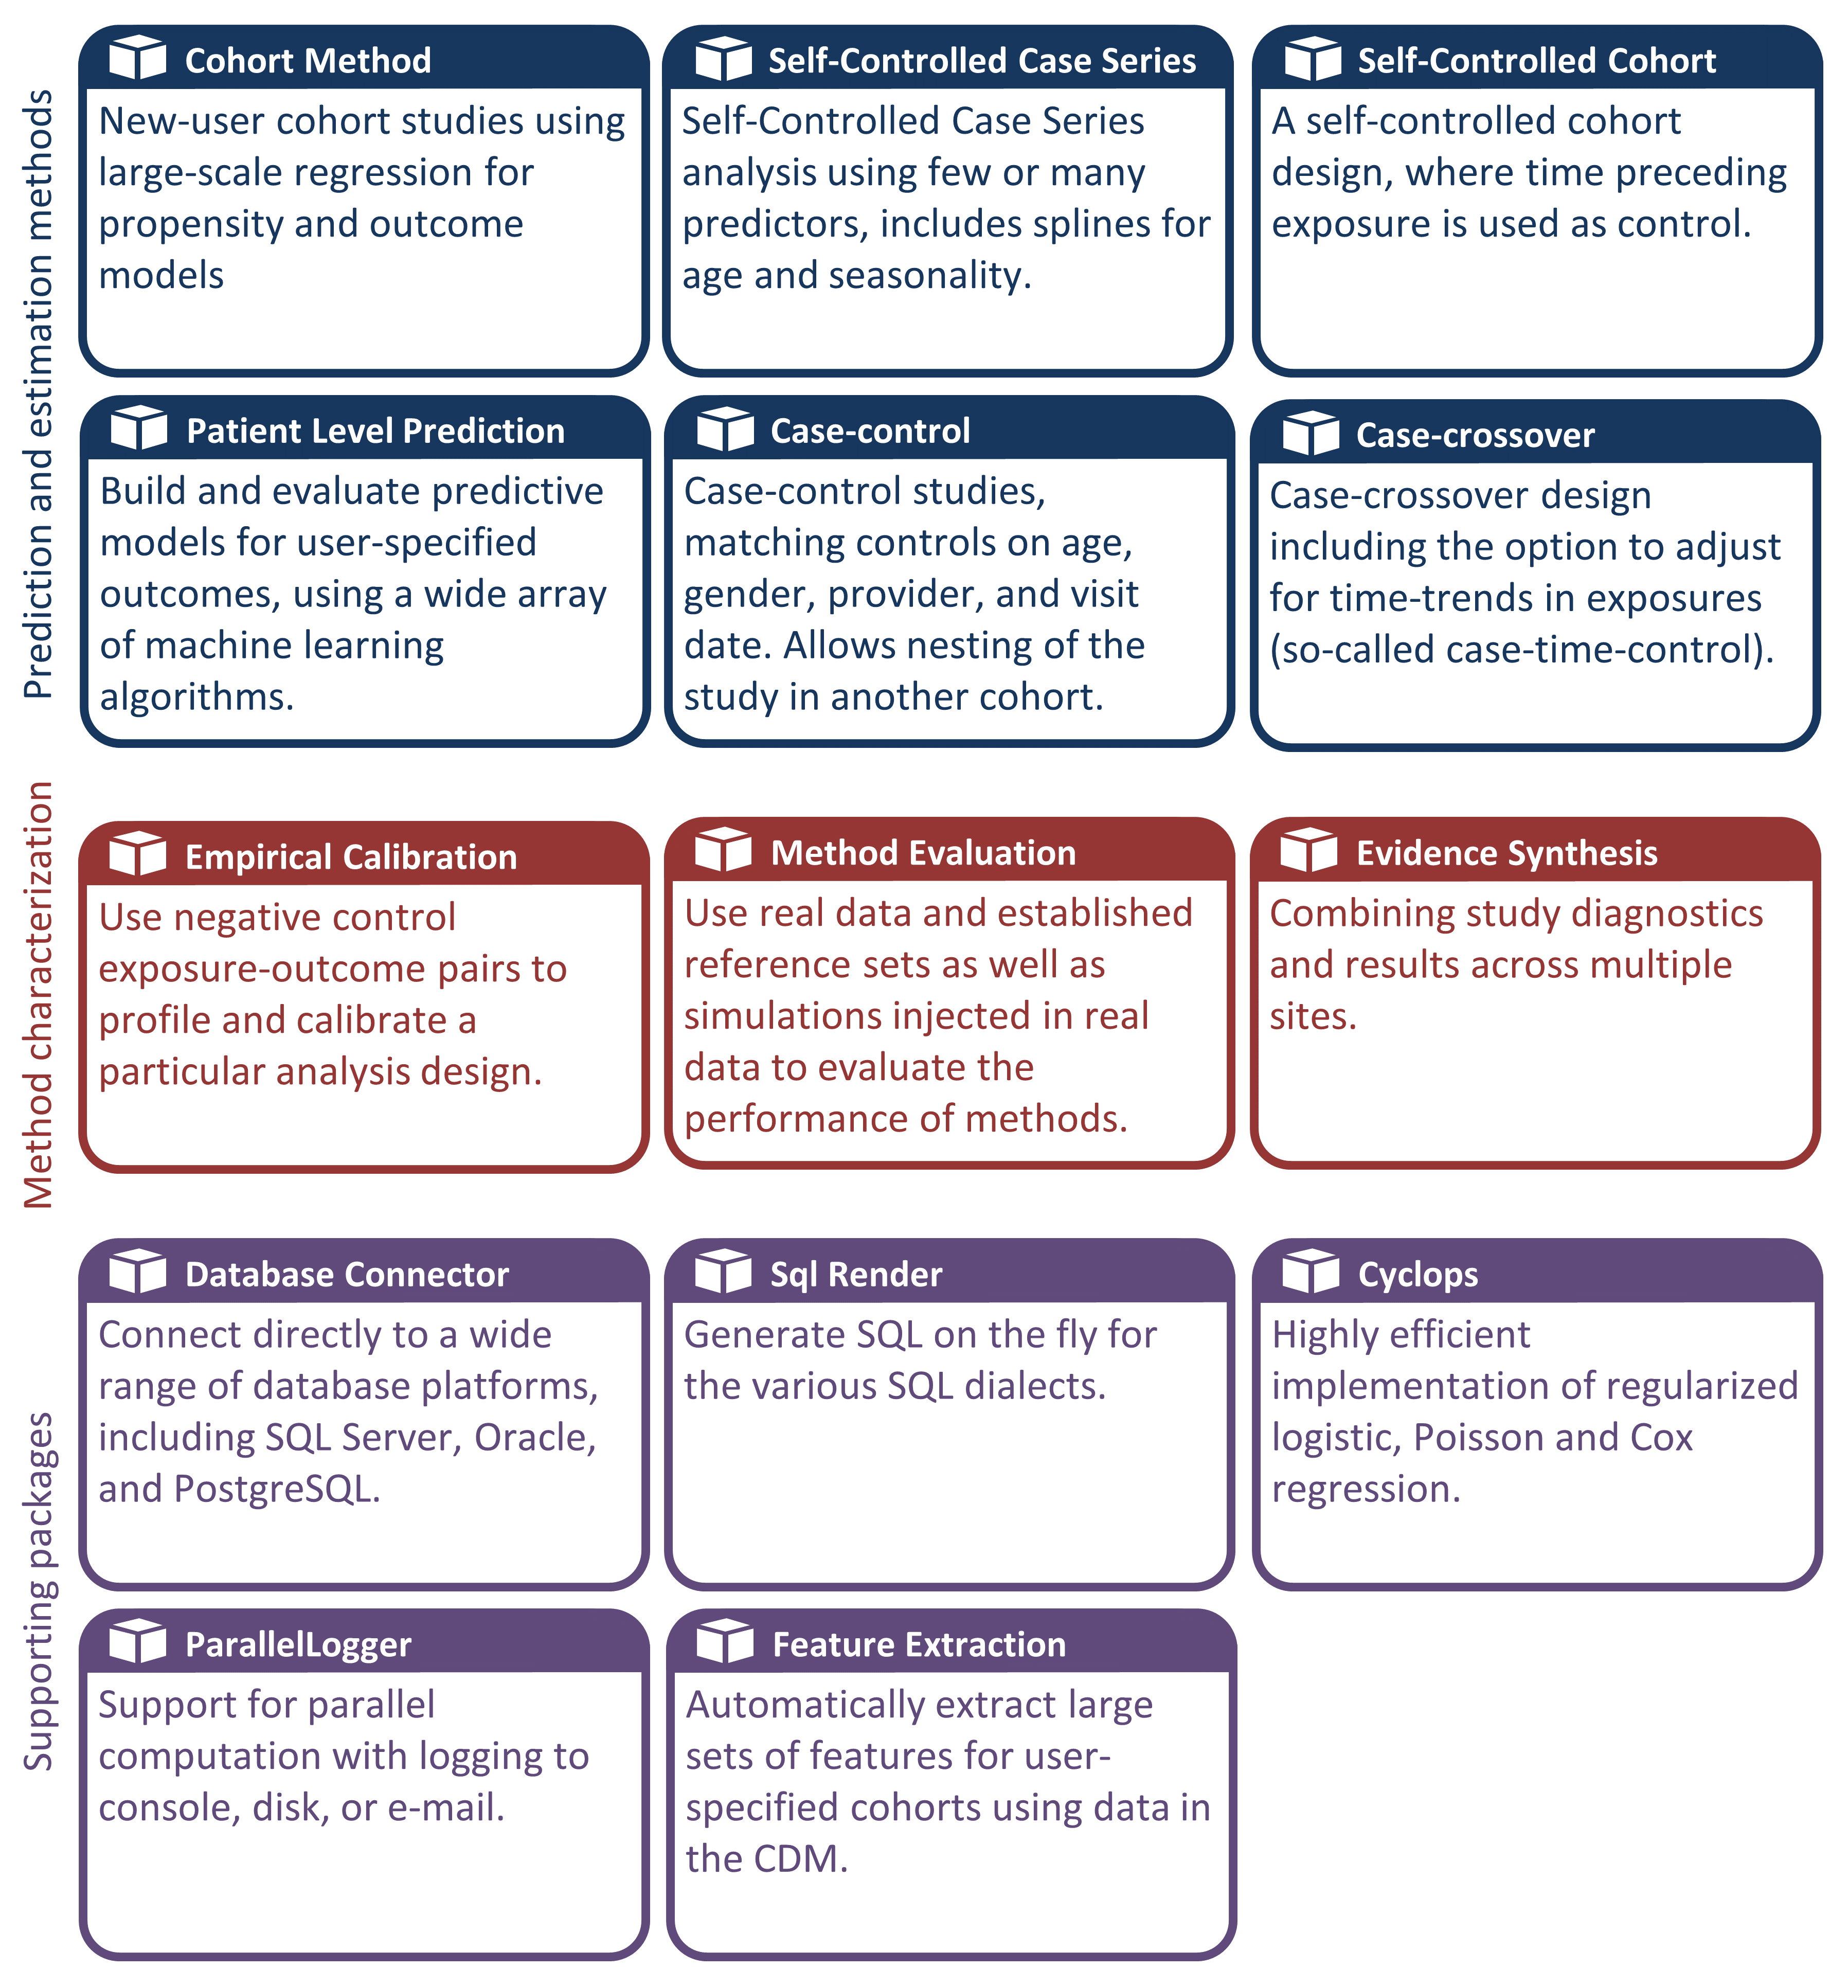
\includegraphics[width=1\linewidth]{images/OhdsiAnalyticsTools/methodsLibrary} 

}

\caption{Packages in the OHDSI Methods Library.}\label{fig:methodsLibrary}
\end{figure}

The packages offer R functions that together can be used to perform a
complete observational study, starting from data in the CDM, and
resulting in estimates and supporting statistics, figures, and tables.
The packages interact directly with observational data in the CDM, and
can be used simply to provide cross-platform compatibility to completely
custom analyses as described in Chapter \ref{SqlAndR}, or can provide
advanced standardized analytics for population characterization (Chapter
\ref{Characterization}), population-level effect estimation (Chapter
\ref{PopulationLevelEstimation}), and patient-level prediction (Chapter
\ref{PatientLevelPrediction}). The Methods Library supports best
practices for use of observational data and observational study design
as learned from previous and ongoing research, such as transparency,
reproducibility, as well as measuring of the operating characteristics
of methods in a particular context and subsequent empirical calibration
of estimates produced by the methods.

The Methods Library has already been used in many published clinical
studies
\citep{boland_2017, duke_2017, ramcharran_2017, weinstein_2017, wang_2017, ryan_2017, ryan_2018, vashisht_2018, yuan_2018, johnston_2019},
as well as methodological studies.
\citep{schuemie_2014, schuemie_2016, reps2018, tian_2018, schuemie_2018, schuemie_2018b, reps_2019}
The validity of the implementations of methods in the Methods library is
described in Chapter \ref{SoftwareValidity}.

\subsection{Support for Large-Scale
Analytics}\label{support-for-large-scale-analytics}

One key feature incorporated in all packages is the ability to
efficiently run many analyses. For example, when performing
population-level estimation, the CohortMethod package allows for
computing effect-size estimates for many exposures and outcomes, using
various analysis settings, and the package will automatically choose the
optimal way to compute all the required intermediary and final data
sets. Steps that can be re-used, such as extraction of covariates, or
fitting a propensity model that is used for one target-comparator pair
but multiple outcomes, will be executed only once. Where possible,
computations will take place in parallel to maximize the use of
computational resources.

This computational efficiency allows for large-scale analytics,
answering many questions at once, and is also essential for including
control hypotheses (e.g.~negative controls) to measure the operating
characteristics of our methods, and perform empirical calibration as
described in Chapter \ref{MethodValidity}. \index{control hypotheses}

\subsection{Support for Big Data}\label{BigDataSupport}

The Methods Library is also designed to run against very large databases
and be able to perform computations involving large amounts of data.
This achieved in three ways:

\begin{enumerate}
\def\labelenumi{\arabic{enumi}.}
\tightlist
\item
  Most data manipulation is performed on the database server. An
  analysis usually only requires a small fraction of the entire data in
  the database, and the Methods Library, through the SqlRender and
  DatabaseConnector packages, allows for advanced operations to be
  performed on the server to preprocess and extract the relevant data.
\item
  Large local data objects are stored in a memory-efficient manner. For
  the data that is downloaded to the local machine, the Methods Library
  uses the \href{https://cran.r-project.org/web/packages/ff}{ff} package
  to store and work with large data objects. This allows us to work with
  data much larger than fits in memory.
\item
  High-performance computing is applied where needed. For example, the
  \href{https://ohdsi.github.io/Cyclops/}{Cyclops} package implements a
  highly efficient regression engine that is used throughout the Methods
  Library to perform large-scale regressions (large number of variables,
  large number of observations) that would not be possible to fit
  otherwise.
\end{enumerate}

\subsection{Documentation}\label{documentation-1}

R provides a standard way to document packages. Each package has a
\emph{package manual} that documents every function and data set
contained in the package. All package manuals are available online
through the Methods Library website\footnote{\url{https://ohdsi.github.io/MethodsLibrary}},
through the package GitHub repositories, and for those packages
available through CRAN they can be found in CRAN. Furthermore, from
within R the package manual can be consulted by using the question mark.
For example, after loading the DatabaseConnector package, typing the
command \texttt{?connect} brings up the documentation on the ``connect''
function.

In addition to the package manual, many packages provide
\emph{vignettes}. Vignettes are long-form documentation that describe
how a package can be used to perform certain tasks. For example, one
vignette\footnote{\url{https://ohdsi.github.io/CohortMethod/articles/MultipleAnalyses.html}}
describes how to perform multiple analyses efficiently using the
CohortMethod package. Vignettes can also be found through the Methods
Library website, through the package GitHub repositories, and for those
packages available through CRAN they can be found in CRAN.
\index{vignette}

\subsection{System Requirements}\label{system-requirements}

Two computing environments are relevant when discussing the system
requirements: The database server, and the analytics workstation.
\index{system requirements}

The database server must hold the observational healthcare data in CDM
format. The Methods Library supports a wide array of database management
systems including traditional database systems (PostgreSQL, Microsoft
SQL Server, and Oracle), parallel data warehouses (Microsoft APS, IBM
Netezza, and Amazon RedShift), as well as Big Data platforms (Hadoop
through Impala, and Google BigQuery).

The analytics workstation is where the Methods Library is installed and
run. This can either be a local machine, such as someone's laptop, or a
remote server running RStudio Server. In all cases the requirements are
that R is installed, preferably together with RStudio. The Methods
Library also requires that Java is installed. The analytics workstation
should also be able to connect to the database server, specifically, any
firewall between them should have the database server access ports
opened the workstation. Some of the analytics can be computationally
intensive, so having multiple processing cores and ample memory can help
speed up the analyses. We recommend having at least four cores and 16
gigabytes of memory.

\subsection{How to Install}\label{installR}

Here are the steps for installing the required environment to run the
OHDSI R packages. Four things need to be installed:
\index{R!installation}

\begin{enumerate}
\def\labelenumi{\arabic{enumi}.}
\tightlist
\item
  \textbf{R} is a statistical computing environment. It comes with a
  basic user interface that is primarily a command-line interface.
\item
  \textbf{RTools} is a set of programs that is required on Windows to
  build R packages from source.
\item
  \textbf{RStudio} is an IDE (Integrated Development Environment) that
  makes R easier to use. It includes a code editor, debugging and
  visualization tools. Please use it to obtain a nice R experience.
\item
  \textbf{Java} is a computing environment that is needed to run some of
  the components in the OHDSI R packages, for example those needed to
  connect to a database.
\end{enumerate}

Below we describe how to install each of these in a Windows environment.

\BeginKnitrBlock{rmdimportant}
In Windows, both R and Java come in 32-bit and 64-bits architectures. If
you install R in both architectures, you \textbf{must} also install Java
in both architectures. It is recommended to only install the 64-bit
version of R.
\EndKnitrBlock{rmdimportant}

\subsubsection*{Installing R}\label{installing-r}
\addcontentsline{toc}{subsubsection}{Installing R}

\begin{enumerate}
\def\labelenumi{\arabic{enumi}.}
\tightlist
\item
  Go to \url{https://cran.r-project.org/}, click on ``Download R for
  Windows'', then ``base'', then click the Download link indicated in
  Figure \ref{fig:downloadR}.
\end{enumerate}

\begin{figure}

{\centering 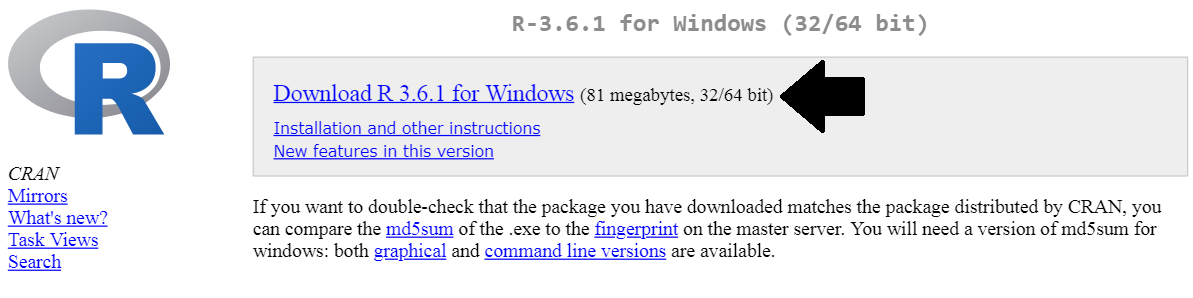
\includegraphics[width=1\linewidth]{images/OhdsiAnalyticsTools/downloadR} 

}

\caption{Downloading R from CRAN.}\label{fig:downloadR}
\end{figure}

\begin{enumerate}
\def\labelenumi{\arabic{enumi}.}
\setcounter{enumi}{1}
\tightlist
\item
  After the download has completed, run the installer. Use the default
  options everywhere, with two exceptions: First, it is better not to
  install into program files. Instead, just make R a subfolder of your C
  drive as shown in Figure \ref{fig:rDestination}. Second, to avoid
  problems due to differing architectures between R and Java, disable
  the 32-bit architecture as shown in Figure \ref{fig:no32Bits}.
\end{enumerate}

\begin{figure}

{\centering 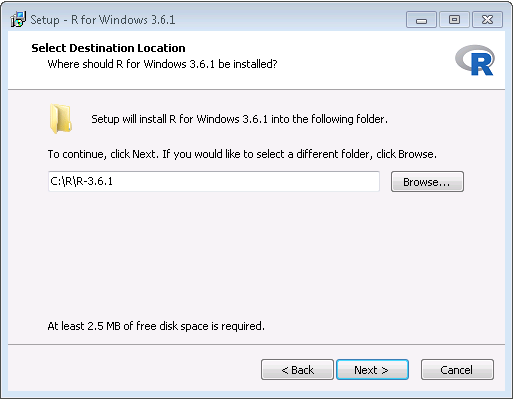
\includegraphics[width=0.8\linewidth]{images/OhdsiAnalyticsTools/rDestination} 

}

\caption{Settings the destination folder for R.}\label{fig:rDestination}
\end{figure}

\begin{figure}

{\centering 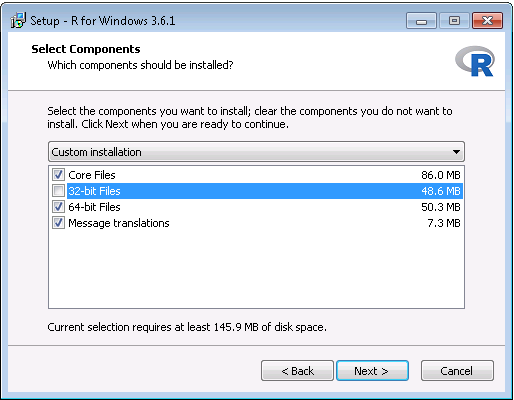
\includegraphics[width=0.8\linewidth]{images/OhdsiAnalyticsTools/no32Bits} 

}

\caption{Disabling the 32-bit version of R.}\label{fig:no32Bits}
\end{figure}

Once completed, you should be able to select R from your Start Menu.

\subsubsection*{Installing RTools}\label{installing-rtools}
\addcontentsline{toc}{subsubsection}{Installing RTools}

\begin{enumerate}
\def\labelenumi{\arabic{enumi}.}
\item
  Go to \url{https://cran.r-project.org/}, click on ``Download R for
  Windows'', then ``Rtools'', and select the very latest version of
  RTools to download.
\item
  After downloading has completed run the installer. Select the default
  options everywhere.
\end{enumerate}

\subsubsection*{Installing RStudio}\label{installing-rstudio}
\addcontentsline{toc}{subsubsection}{Installing RStudio}

\begin{enumerate}
\def\labelenumi{\arabic{enumi}.}
\tightlist
\item
  Go to \url{https://www.rstudio.com/}, select ``Download RStudio'' (or
  the ``Download'' button under ``RStudio''), opt for the free version,
  and download the installer for Windows as shown in Figure
  \ref{fig:downloadRStudio}.
\end{enumerate}

\begin{figure}

{\centering 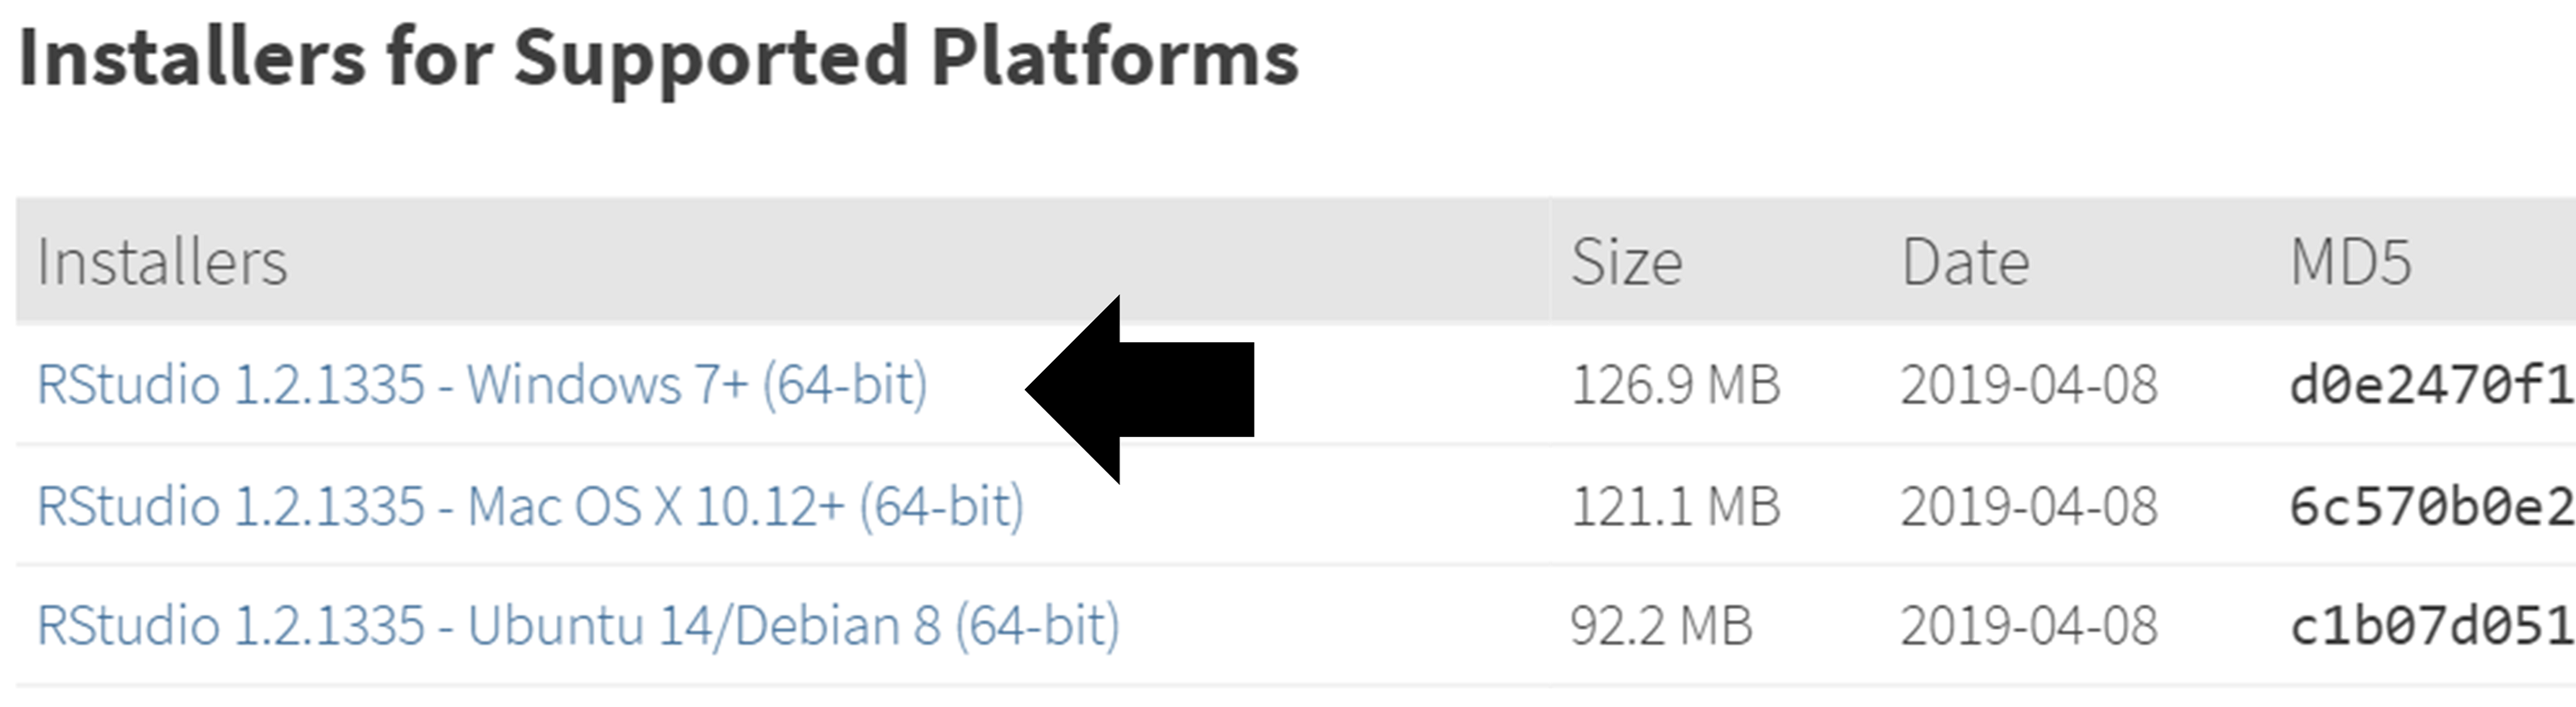
\includegraphics[width=1\linewidth]{images/OhdsiAnalyticsTools/downloadRStudio} 

}

\caption{Downloading RStudio.}\label{fig:downloadRStudio}
\end{figure}

\begin{enumerate}
\def\labelenumi{\arabic{enumi}.}
\setcounter{enumi}{1}
\tightlist
\item
  After downloading, start the installer, and use the default options
  everywhere.
\end{enumerate}

\subsubsection*{Installing Java}\label{installing-java}
\addcontentsline{toc}{subsubsection}{Installing Java}

\begin{enumerate}
\def\labelenumi{\arabic{enumi}.}
\tightlist
\item
  Go to \url{https://java.com/en/download/manual.jsp}, and select the
  Windows 64-bit installer as shown in Figure \ref{fig:downloadJava}. If
  you also installed the 32-bit version of R, you \emph{must} also
  install the other (32-bit) version of Java.
\end{enumerate}

\begin{figure}

{\centering 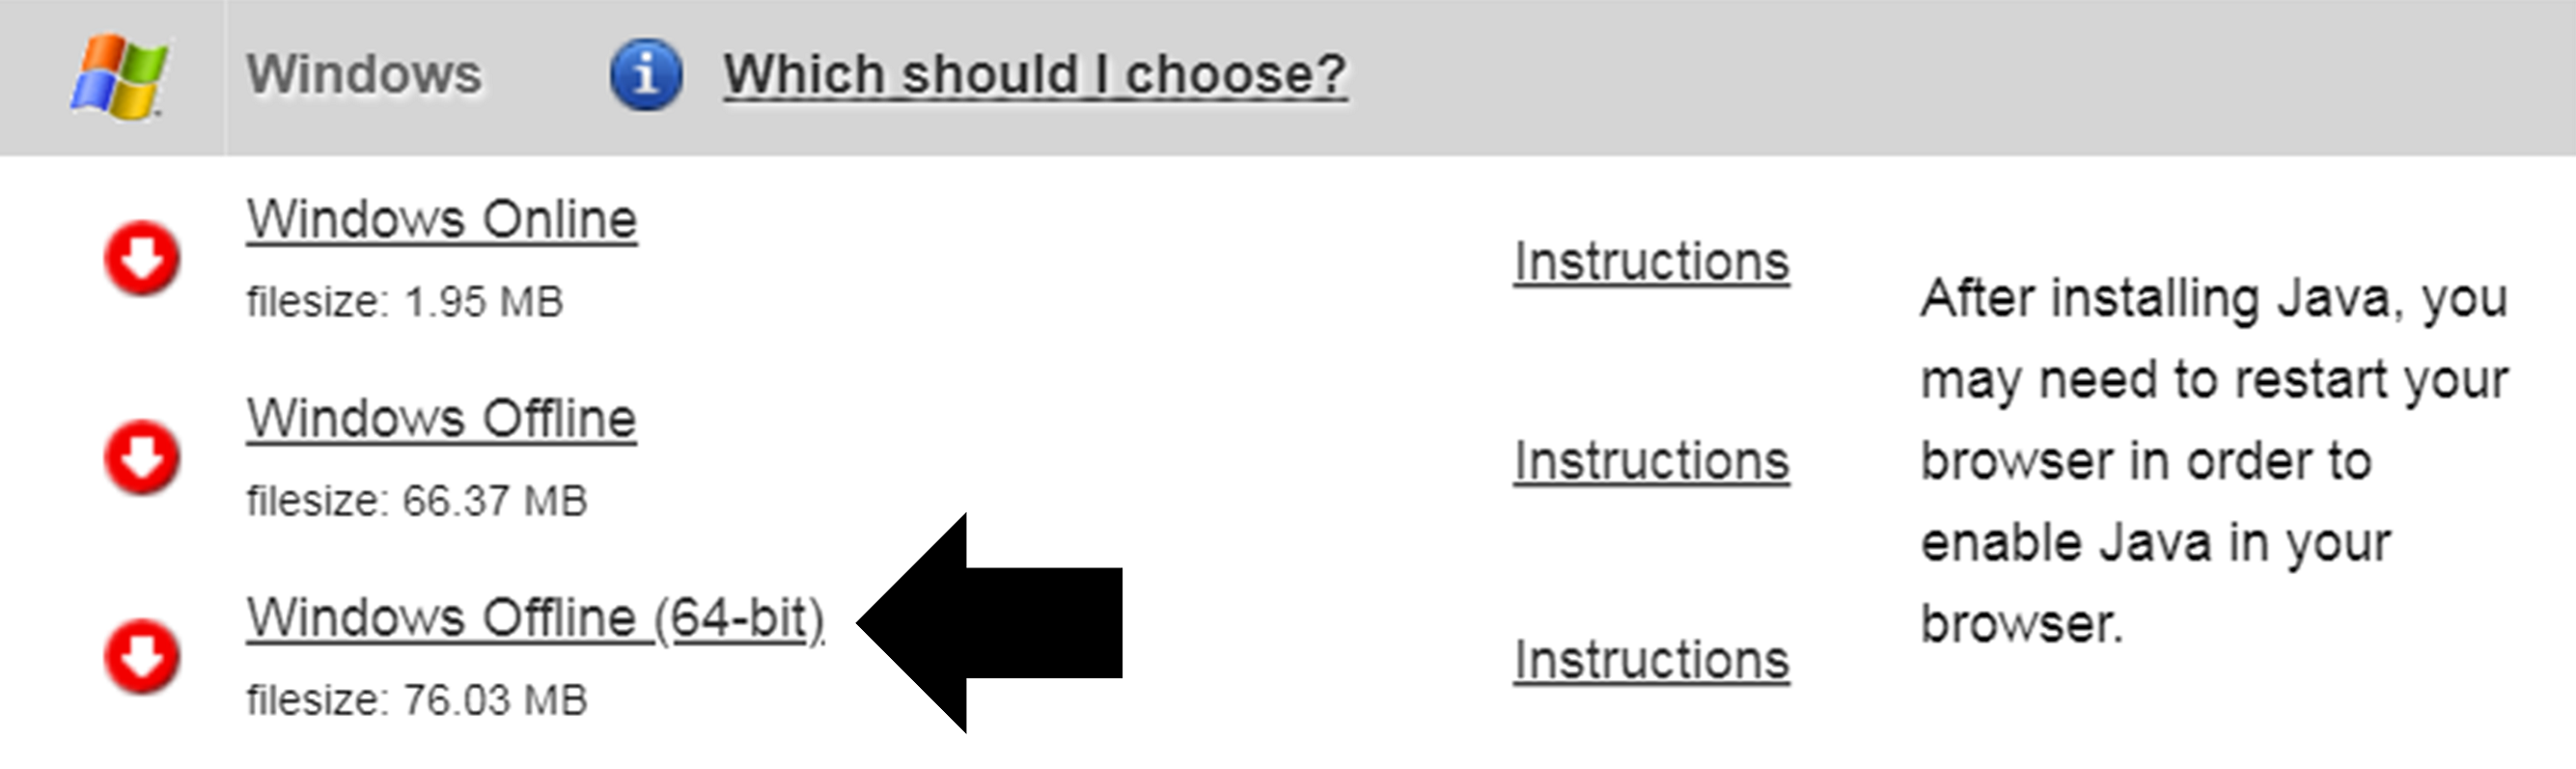
\includegraphics[width=1\linewidth]{images/OhdsiAnalyticsTools/downloadJava} 

}

\caption{Downloading Java.}\label{fig:downloadJava}
\end{figure}

\begin{enumerate}
\def\labelenumi{\arabic{enumi}.}
\setcounter{enumi}{1}
\tightlist
\item
  After downloading just run the installer.
\end{enumerate}

\subsubsection*{Verifying the
Installation}\label{verifying-the-installation}
\addcontentsline{toc}{subsubsection}{Verifying the Installation}

You should now be ready to go, but we should make sure. Start RStudio,
and type

\begin{Shaded}
\begin{Highlighting}[]
\KeywordTok{install.packages}\NormalTok{(}\StringTok{"SqlRender"}\NormalTok{)}
\KeywordTok{library}\NormalTok{(SqlRender)}
\KeywordTok{translate}\NormalTok{(}\StringTok{"SELECT TOP 10 * FROM person;"}\NormalTok{, }\StringTok{"postgresql"}\NormalTok{)}
\end{Highlighting}
\end{Shaded}

\begin{verbatim}
## [1] "SELECT  * FROM person LIMIT 10;"
\end{verbatim}

This function uses Java, so if all goes well we know both R and Java
have been installed correctly!

Another test is to see if source packages can be built. Run the
following R code to install the \texttt{CohortMethod} package from the
OHDSI GitHub repository:

\begin{Shaded}
\begin{Highlighting}[]
\KeywordTok{install.packages}\NormalTok{(}\StringTok{"drat"}\NormalTok{)}
\NormalTok{drat}\OperatorTok{::}\KeywordTok{addRepo}\NormalTok{(}\StringTok{"OHDSI"}\NormalTok{)}
\KeywordTok{install.packages}\NormalTok{(}\StringTok{"CohortMethod"}\NormalTok{)}
\end{Highlighting}
\end{Shaded}

\section{Deployment Strategies}\label{deployment-strategies}

Deploying the entire OHDSI tool stack, including ATLAS and the Methods
Library, in an organization is a daunting task. There are many
components with dependencies that have to be considered, and
configurations to set. For this reason, two initiatives have developed
integrated deployment strategies that allow the entire stack to be
installed as one package, using some forms of virtualization: Broadsea
and Amazon Web Services (AWS). \index{tools deployment}

\subsection{Broadsea}\label{broadsea}

Broadsea\footnote{\url{https://github.com/OHDSI/Broadsea}} uses Docker
container technology.\footnote{\url{https://www.docker.com/}} The OHDSI
tools are packaged along with dependencies into a single portable binary
file called a Docker Image. This image can then be run on a Docker
engine service, creating a virtual machine with all the software
installed and ready to run. Docker engines are available for most
operating systems, including Microsoft Windows, MacOS, and Linux. The
Broadsea Docker image contains the main OHDSI tools, including the
Methods Library and ATLAS. \index{tools deployment!Broadsea}

\subsection{Amazon AWS}\label{amazon-aws}

Amazon has prepared two environments that can be instantiated in the AWS
cloud computing environment with a click of the button:
OHDSI-in-a-Box\footnote{\url{https://github.com/OHDSI/OHDSI-in-a-Box}}
and OHDSIonAWS.\footnote{\url{https://github.com/OHDSI/OHDSIonAWS}}
\index{tools deployment!Amazon AWS}

OHDSI-in-a-Box is specifically created as a learning environment, and is
used in most of the tutorials provided by the OHDSI community. It
includes many OHDSI tools, sample data sets, RStudio and other
supporting software in a single, low cost Windows virtual machine. A
PostgreSQL database is used to store the CDM and also to store the
intermediary results from ATLAS. The OMOP CDM data mapping and ETL tools
are also included in OHDSI-in-a-Box. The architecture for OHDSI-in-a-Box
is depicted in Figure \ref{fig:ohdsiinaboxDiagram}.

\begin{figure}

{\centering 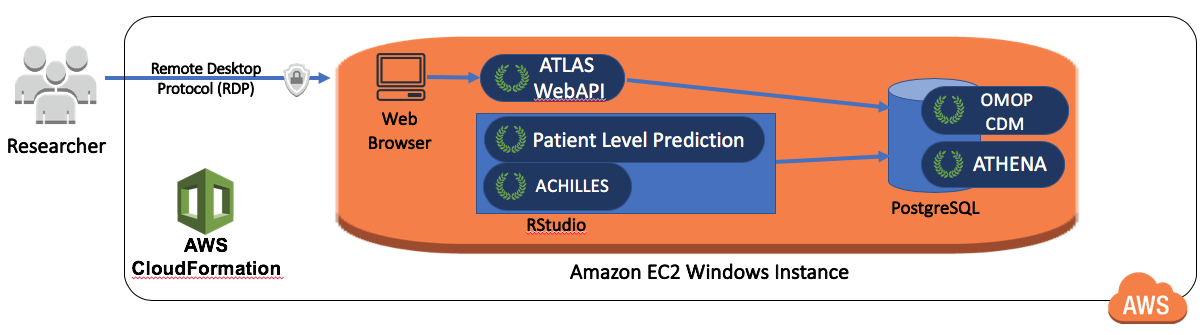
\includegraphics[width=1\linewidth]{images/OhdsiAnalyticsTools/OHDSI-in-a-BoxDiagram} 

}

\caption{The Amazon Web Services architecture for OHDSI-in-a-Box.}\label{fig:ohdsiinaboxDiagram}
\end{figure}

OHDSIonAWS is a reference architecture for enterprise class, multi-user,
scalable and fault tolerant OHDSI environments that can be used by
organizations to perform their data analytics. It includes several
sample datasets and can also automatically load your organization's real
healthcare data. The data is placed in the Amazon Redshift database
platform, which is supported by the OHDSI tools. Intermediary results of
ATLAS are stored in a PostgreSQL database. On the front end, users have
access to ATLAS and to RStudio through a web interface (leveraging
RStudio Server). In RStudio the OHDSI Methods Library has already been
installed, and can be used to connect to the databases. The automation
to deploy OHDSIonAWS is open-source, and can be customized to include
your organization's management tools and best practices. The
architecture for OHDSIonAWS is depicted in Figure
\ref{fig:ohdsionawsDiagram}.

\begin{figure}

{\centering 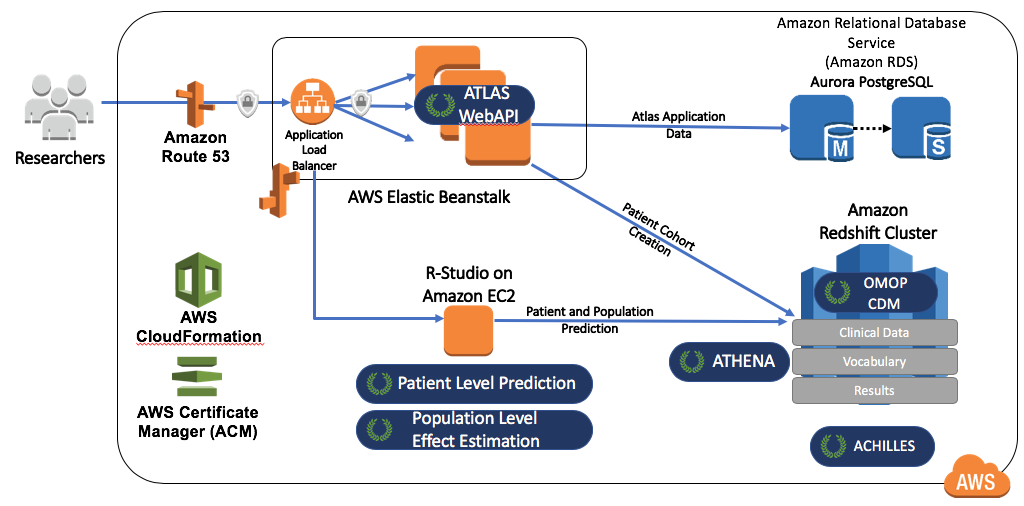
\includegraphics[width=1\linewidth]{images/OhdsiAnalyticsTools/OHDSIonAWSDiagram} 

}

\caption{The Amazon Web Services architecure for OHDSIonAWS.}\label{fig:ohdsionawsDiagram}
\end{figure}

\section{Summary}\label{summary-6}

\BeginKnitrBlock{rmdsummary}
\begin{itemize}
\tightlist
\item
  We can perform analyses against data in the CDM by

  \begin{itemize}
  \tightlist
  \item
    writing custom code
  \item
    writing code that uses the R packages in the OHDSI Methods Library
  \item
    using the interactive analysis platform ATLAS
  \end{itemize}
\item
  OHDSI tools use different analysis strategies

  \begin{itemize}
  \tightlist
  \item
    Single studies
  \item
    Real-time queries
  \item
    Large-scale analytics
  \end{itemize}
\item
  The majority of OHDSI analytics tool are embedded in

  \begin{itemize}
  \tightlist
  \item
    The interactive analysis platform ATLAS
  \item
    The OHDSI Methods Library R packages
  \end{itemize}
\item
  Several strategies exist facilitating the deployment of the OHDSI
  tools.
\end{itemize}
\EndKnitrBlock{rmdsummary}

\chapter{SQL and R}\label{SqlAndR}

\emph{Chapter leads: Martijn Schuemie \& Peter Rijnbeek}

The Common Data Model (CDM) is a relational database model (all data is
represented as records in tables that have fields), which means that the
data will typically be stored in a relational database using a software
platform like PostgreSQL, Oracle, or Microsoft SQL Server. The various
OHDSI tools such as ATLAS and the Methods Library work by querying the
database behind the scene, but we can also query the database directly
ourselves if we have appropriate access rights. The main reason to do
this is to perform analyses that currently are not supported by any
existing tool. However, directly querying the database also comes with
greater risk of making mistakes, as the OHDSI tools are often designed
to help guide the user to appropriate analysis of the data. Direct
queries do not provide such guidance.

The standard language for querying relational databases is SQL
(Structured Query Language), which can be used both to query the
database as well as to make changes to the data. Although the basic
commands in SQL are indeed standard, meaning the same across software
platforms, each platform has its own dialect, with subtle changes. For
example, to retrieve the top 10 rows of the PERSON table on SQL Server,
one would type: \index{SQL} \index{structured query language|see {SQL}}

\begin{Shaded}
\begin{Highlighting}[]
\KeywordTok{SELECT}\NormalTok{ TOP }\DecValTok{10}\NormalTok{ * }\KeywordTok{FROM}\NormalTok{ person;}
\end{Highlighting}
\end{Shaded}

Whereas the same query on PostgreSQL would be:

\begin{Shaded}
\begin{Highlighting}[]
\KeywordTok{SELECT}\NormalTok{ * }\KeywordTok{FROM}\NormalTok{ person }\KeywordTok{LIMIT} \DecValTok{10}\NormalTok{;}
\end{Highlighting}
\end{Shaded}

In OHDSI, we would like to be agnostic to the specific dialect a
platform uses; we would like to `speak' the same SQL language across all
OHDSI databases. For this reason OHDSI developed the
\href{https://ohdsi.github.io/SqlRender/}{SqlRender} package, an R
package that can translate from one standard dialect to any of the
supported dialects that will be discussed later in this chapter. This
standard dialect - \textbf{OHDSI SQL} - is mainly a subset of the SQL
Server SQL dialect. The example SQL statements provided throughout this
chapter will all use OHDSI SQL. \index{SqlRender}
\index{agnostic SQL|see {SqlRender}}
\index{Standard SQL Dialect|see {SqlRender}}
\index{OHDSI SQL|see {SqlRender}}

Each database platform also comes with its own software tools for
querying the database using SQL. In OHDSI we developed the
\href{https://ohdsi.github.io/DatabaseConnector/}{DatabaseConnector}
package, one R package that can connect to many database platforms.
DatabaseConnector will also be discussed later in this chapter.
\index{DatabaseConnector}

So although one can query a database that conforms to the CDM without
using any OHDSI tools, the recommended path is to use the
DatabaseConnector and SqlRender packages. This allows queries that are
developed at one site to be used at any other site without modification.
R itself also immediately provides features to further analyze the data
extracted from the database, such as performing statistical analyses and
generating (interactive) plots. \index{R}

In this chapter we assume the reader has a basic understanding of SQL.
We first review how to use SqlRender and DatabaseConnector. If the
reader does not intend to use these packages these sections can be
skipped. In Section \ref{QueryTheCdm} we discuss how to use SQL (in this
case OHDSI SQL) to query the CDM. The following section highlights how
to use the OHDSI Standardized Vocabulary when querying the CDM. We
highlight the QueryLibrary, a collection of commonly-used queries
against the CDM that is publicly available. We close this chapter with
an example study estimating incidence rates, and implement this study
using SqlRender and DatabaseConnector. \index{Query Library}
\index{SQL Query Libary|see {Query Library}}

\section{SqlRender}\label{SqlRender}

The \href{https://ohdsi.github.io/SqlRender/}{SqlRender} package is
available on CRAN (the Comprehensive R Archive Network), and can
therefore be installed using:

\begin{Shaded}
\begin{Highlighting}[]
\KeywordTok{install.packages}\NormalTok{(}\StringTok{"SqlRender"}\NormalTok{)}
\end{Highlighting}
\end{Shaded}

SqlRender supports a wide array of technical platforms including
traditional database systems (PostgreSQL, Microsoft SQL Server, SQLite,
and Oracle), parallel data warehouses (Microsoft APS, IBM Netezza, and
Amazon RedShift), as well as Big Data platforms (Hadoop through Impala,
and Google BigQuery). The R package comes with a package manual and a
vignette that explores the full functionality. Here we describer some of
the main features.

\subsection{SQL Parameterization}\label{sql-parameterization}

One of the functions of the package is to support parameterization of
SQL. Often, small variations of SQL need to be generated based on some
parameters. SqlRender offers a simple markup syntax inside the SQL code
to allow parameterization. Rendering the SQL based on parameter values
is done using the \texttt{render()} function.
\index{SqlRender!parameterization}

\subsubsection*{Substituting Parameter
Values}\label{substituting-parameter-values}
\addcontentsline{toc}{subsubsection}{Substituting Parameter Values}

The \texttt{@} character can be used to indicate parameter names that
need to be exchanged for actual parameter values when rendering. In the
following example, a variable called \texttt{a} is mentioned in the SQL.
In the call to the render function the value of this parameter is
defined:

\begin{Shaded}
\begin{Highlighting}[]
\NormalTok{sql <-}\StringTok{ "SELECT * FROM concept WHERE concept_id = @a;"}
\KeywordTok{render}\NormalTok{(sql, }\DataTypeTok{a =} \DecValTok{123}\NormalTok{)}
\end{Highlighting}
\end{Shaded}

\begin{verbatim}
## [1] "SELECT * FROM concept WHERE concept_id = 123;"
\end{verbatim}

Note that, unlike the parameterization offered by most database
management systems, it is just as easy to parameterize table or field
names as values:

\begin{Shaded}
\begin{Highlighting}[]
\NormalTok{sql <-}\StringTok{ "SELECT * FROM @x WHERE person_id = @a;"}
\KeywordTok{render}\NormalTok{(sql, }\DataTypeTok{x =} \StringTok{"observation"}\NormalTok{, }\DataTypeTok{a =} \DecValTok{123}\NormalTok{)}
\end{Highlighting}
\end{Shaded}

\begin{verbatim}
## [1] "SELECT * FROM observation WHERE person_id = 123;"
\end{verbatim}

The parameter values can be numbers, strings, booleans, as well as
vectors, which are converted to comma-delimited lists:

\begin{Shaded}
\begin{Highlighting}[]
\NormalTok{sql <-}\StringTok{ "SELECT * FROM concept WHERE concept_id IN (@a);"}
\KeywordTok{render}\NormalTok{(sql, }\DataTypeTok{a =} \KeywordTok{c}\NormalTok{(}\DecValTok{123}\NormalTok{, }\DecValTok{234}\NormalTok{, }\DecValTok{345}\NormalTok{))}
\end{Highlighting}
\end{Shaded}

\begin{verbatim}
## [1] "SELECT * FROM concept WHERE concept_id IN (123,234,345);"
\end{verbatim}

\subsubsection*{If-Then-Else}\label{if-then-else}
\addcontentsline{toc}{subsubsection}{If-Then-Else}

Sometimes blocks of codes need to be turned on or off based on the
values of one or more parameters. This is done using the
\texttt{\{Condition\}\ ?\ \{if\ true\}\ :\ \{if\ false\}} syntax. If the
\emph{condition} evaluates to true or 1, the \emph{if true} block is
used, else the \emph{if false} block is shown (if present).

\begin{Shaded}
\begin{Highlighting}[]
\NormalTok{sql <-}\StringTok{ "SELECT * FROM cohort \{@x\} ? \{WHERE subject_id = 1\}"}
\KeywordTok{render}\NormalTok{(sql, }\DataTypeTok{x =} \OtherTok{FALSE}\NormalTok{)}
\end{Highlighting}
\end{Shaded}

\begin{verbatim}
## [1] "SELECT * FROM cohort "
\end{verbatim}

\begin{Shaded}
\begin{Highlighting}[]
\KeywordTok{render}\NormalTok{(sql, }\DataTypeTok{x =} \OtherTok{TRUE}\NormalTok{)}
\end{Highlighting}
\end{Shaded}

\begin{verbatim}
## [1] "SELECT * FROM cohort WHERE subject_id = 1"
\end{verbatim}

Simple comparisons are also supported:

\begin{Shaded}
\begin{Highlighting}[]
\NormalTok{sql <-}\StringTok{ "SELECT * FROM cohort \{@x == 1\} ? \{WHERE subject_id = 1\};"}
\KeywordTok{render}\NormalTok{(sql, }\DataTypeTok{x =} \DecValTok{1}\NormalTok{)}
\end{Highlighting}
\end{Shaded}

\begin{verbatim}
## [1] "SELECT * FROM cohort WHERE subject_id = 1;"
\end{verbatim}

\begin{Shaded}
\begin{Highlighting}[]
\KeywordTok{render}\NormalTok{(sql, }\DataTypeTok{x =} \DecValTok{2}\NormalTok{)}
\end{Highlighting}
\end{Shaded}

\begin{verbatim}
## [1] "SELECT * FROM cohort ;"
\end{verbatim}

As well as the \texttt{IN} operator:

\begin{Shaded}
\begin{Highlighting}[]
\NormalTok{sql <-}\StringTok{ "SELECT * FROM cohort \{@x IN (1,2,3)\} ? \{WHERE subject_id = 1\};"}
\KeywordTok{render}\NormalTok{(sql, }\DataTypeTok{x =} \DecValTok{2}\NormalTok{)}
\end{Highlighting}
\end{Shaded}

\begin{verbatim}
## [1] "SELECT * FROM cohort WHERE subject_id = 1;"
\end{verbatim}

\subsection{Translation to Other SQL
Dialects}\label{translation-to-other-sql-dialects}

Another function of the
\href{https://ohdsi.github.io/SqlRender/}{SqlRender} package is to
translate from OHDSI SQL to other SQL dialects. For example:

\begin{Shaded}
\begin{Highlighting}[]
\NormalTok{sql <-}\StringTok{ "SELECT TOP 10 * FROM person;"}
\KeywordTok{translate}\NormalTok{(sql, }\DataTypeTok{targetDialect =} \StringTok{"postgresql"}\NormalTok{)}
\end{Highlighting}
\end{Shaded}

\begin{verbatim}
## [1] "SELECT  * FROM person LIMIT 10;"
\end{verbatim}

The \texttt{targetDialect} parameter can have the following values:
``oracle'', ``postgresql'', ``pdw'', ``redshift'', ``impala'',
``netezza'', ``bigquery'', ``sqlite'', and ``sql server''.
\index{SqlRender!translation}

\BeginKnitrBlock{rmdimportant}
There are limits to what SQL functions and constructs can be translated
properly, both because only a limited set of translation rules have been
implemented in the package, but also some SQL features do not have an
equivalent in all dialects. This is the primary reason why OHDSI SQL was
developed as its own, new SQL dialect. However, whenever possible we
have kept to the SQL Server syntax to avoid reinventing the wheel.
\EndKnitrBlock{rmdimportant}

Despite our best efforts, there are quite a few things to consider when
writing OHDSI SQL that will run without error on all supported
platforms. In what follows we discuss these considerations in detail.

\subsubsection*{Functions and Structures Supported By
Translate}\label{functions-and-structures-supported-by-translate}
\addcontentsline{toc}{subsubsection}{Functions and Structures Supported
By Translate}

These SQL Server functions have been tested and were found to be
translated correctly to the various
dialects:\index{SqlRender!supported functions}

\begin{longtable}[]{@{}lll@{}}
\caption{\label{tab:sqlFunctions} Functions supported by
translate.}\tabularnewline
\toprule
Function & Function & Function\tabularnewline
\midrule
\endfirsthead
\toprule
Function & Function & Function\tabularnewline
\midrule
\endhead
ABS & EXP & RAND\tabularnewline
ACOS & FLOOR & RANK\tabularnewline
ASIN & GETDATE & RIGHT\tabularnewline
ATAN & HASHBYTES* & ROUND\tabularnewline
AVG & ISNULL & ROW\_NUMBER\tabularnewline
CAST & ISNUMERIC & RTRIM\tabularnewline
CEILING & LEFT & SIN\tabularnewline
CHARINDEX & LEN & SQRT\tabularnewline
CONCAT & LOG & SQUARE\tabularnewline
COS & LOG10 & STDEV\tabularnewline
COUNT & LOWER & SUM\tabularnewline
COUNT\_BIG & LTRIM & TAN\tabularnewline
DATEADD & MAX & UPPER\tabularnewline
DATEDIFF & MIN & VAR\tabularnewline
DATEFROMPARTS & MONTH & YEAR\tabularnewline
DATETIMEFROMPARTS & NEWID &\tabularnewline
DAY & PI &\tabularnewline
EOMONTH & POWER &\tabularnewline
\bottomrule
\end{longtable}

* Requires special privileges on Oracle. Has no equivalent on SQLite.

Similarly, many SQL syntax structures are supported. Here is a
non-exhaustive list of expressions that we know will translate well:

\begin{Shaded}
\begin{Highlighting}[]
\CommentTok{-- Simple selects:}
\KeywordTok{SELECT}\NormalTok{ * }\KeywordTok{FROM} \KeywordTok{table}\NormalTok{;}

\CommentTok{-- Selects with joins:}
\KeywordTok{SELECT}\NormalTok{ * }\KeywordTok{FROM}\NormalTok{ table_1 }\KeywordTok{INNER} \KeywordTok{JOIN}\NormalTok{ table_2 }\KeywordTok{ON}\NormalTok{ a = b;}

\CommentTok{-- Nested queries:}
\KeywordTok{SELECT}\NormalTok{ * }\KeywordTok{FROM}\NormalTok{ (}\KeywordTok{SELECT}\NormalTok{ * }\KeywordTok{FROM}\NormalTok{ table_1) tmp }\KeywordTok{WHERE}\NormalTok{ a = b;}

\CommentTok{-- Limiting to top rows:}
\KeywordTok{SELECT}\NormalTok{ TOP }\DecValTok{10}\NormalTok{ * }\KeywordTok{FROM} \KeywordTok{table}\NormalTok{;}

\CommentTok{-- Selecting into a new table:}
\KeywordTok{SELECT}\NormalTok{ * }\KeywordTok{INTO}\NormalTok{ new_table }\KeywordTok{FROM} \KeywordTok{table}\NormalTok{;}

\CommentTok{-- Creating tables:}
\KeywordTok{CREATE} \KeywordTok{TABLE} \KeywordTok{table}\NormalTok{ (field }\DataTypeTok{INT}\NormalTok{);}

\CommentTok{-- Inserting verbatim values:}
\KeywordTok{INSERT} \KeywordTok{INTO}\NormalTok{ other_table (field_1) }\KeywordTok{VALUES}\NormalTok{ (}\DecValTok{1}\NormalTok{);}

\CommentTok{-- Inserting from SELECT:}
\KeywordTok{INSERT} \KeywordTok{INTO}\NormalTok{ other_table (field_1) }\KeywordTok{SELECT} \FunctionTok{value} \KeywordTok{FROM} \KeywordTok{table}\NormalTok{;}
  
\CommentTok{-- Simple drop commands:}
\KeywordTok{DROP} \KeywordTok{TABLE} \KeywordTok{table}\NormalTok{;}

\CommentTok{-- Drop table if it exists:}
\KeywordTok{IF}\NormalTok{ OBJECT_ID(}\StringTok{'ACHILLES_analysis'}\NormalTok{, }\StringTok{'U'}\NormalTok{) }\KeywordTok{IS} \KeywordTok{NOT} \KeywordTok{NULL}
  \KeywordTok{DROP} \KeywordTok{TABLE}\NormalTok{ ACHILLES_analysis;}
  
\CommentTok{-- Drop temp table if it exists:}
\KeywordTok{IF}\NormalTok{ OBJECT_ID(}\StringTok{'tempdb..#cohorts'}\NormalTok{, }\StringTok{'U'}\NormalTok{) }\KeywordTok{IS} \KeywordTok{NOT} \KeywordTok{NULL}
  \KeywordTok{DROP} \KeywordTok{TABLE}\NormalTok{ #cohorts;  }

\CommentTok{-- Common table expressions:}
\KeywordTok{WITH}\NormalTok{ cte }\KeywordTok{AS}\NormalTok{ (}\KeywordTok{SELECT}\NormalTok{ * }\KeywordTok{FROM} \KeywordTok{table}\NormalTok{) }\KeywordTok{SELECT}\NormalTok{ * }\KeywordTok{FROM}\NormalTok{ cte;}

\CommentTok{-- OVER clauses:}
\KeywordTok{SELECT} \FunctionTok{ROW_NUMBER}\NormalTok{() }\KeywordTok{OVER}\NormalTok{ (}\KeywordTok{PARTITION} \KeywordTok{BY}\NormalTok{ a }\KeywordTok{ORDER} \KeywordTok{BY}\NormalTok{ b)}
  \KeywordTok{AS} \OtherTok{"Row Number"} \KeywordTok{FROM} \KeywordTok{table}\NormalTok{;}
  
\CommentTok{-- CASE WHEN clauses:}
\KeywordTok{SELECT} \KeywordTok{CASE} \KeywordTok{WHEN}\NormalTok{ a=}\DecValTok{1} \KeywordTok{THEN}\NormalTok{ a }\KeywordTok{ELSE} \DecValTok{0} \KeywordTok{END} \KeywordTok{AS} \FunctionTok{value} \KeywordTok{FROM} \KeywordTok{table}\NormalTok{;}

\CommentTok{-- UNIONs:}
\KeywordTok{SELECT}\NormalTok{ * }\KeywordTok{FROM}\NormalTok{ a }\KeywordTok{UNION} \KeywordTok{SELECT}\NormalTok{ * }\KeywordTok{FROM}\NormalTok{ b;}

\CommentTok{-- INTERSECTIONs:}
\KeywordTok{SELECT}\NormalTok{ * }\KeywordTok{FROM}\NormalTok{ a }\KeywordTok{INTERSECT} \KeywordTok{SELECT}\NormalTok{ * }\KeywordTok{FROM}\NormalTok{ b;}

\CommentTok{-- EXCEPT:}
\KeywordTok{SELECT}\NormalTok{ * }\KeywordTok{FROM}\NormalTok{ a }\KeywordTok{EXCEPT} \KeywordTok{SELECT}\NormalTok{ * }\KeywordTok{FROM}\NormalTok{ b;}
\end{Highlighting}
\end{Shaded}

\subsubsection*{String Concatenation}\label{string-concatenation}
\addcontentsline{toc}{subsubsection}{String Concatenation}

String concatenation is one area where SQL Server is less specific than
other dialects. In SQL Server, one would write
\texttt{SELECT\ first\_name\ +\ \textquotesingle{}\ \textquotesingle{}\ +\ last\_name\ AS\ full\_name\ FROM\ table},
but this should be
\texttt{SELECT\ first\_name\ \textbar{}\textbar{}\ \textquotesingle{}\ \textquotesingle{}\ \textbar{}\textbar{}\ last\_name\ AS\ full\_name\ FROM\ table}
in PostgreSQL and Oracle. SqlRender tries to guess when values that are
being concatenated are strings. In the example above, because we have an
explicit string (the space surrounded by single quotation marks), the
translation will be correct. However, if the query had been
\texttt{SELECT\ first\_name\ +\ last\_name\ AS\ full\_name\ FROM\ table},
SqlRender would have had no clue the two fields were strings, and would
incorrectly leave the plus sign. Another clue that a value is a string
is an explicit cast to VARCHAR, so
\texttt{SELECT\ last\_name\ +\ CAST(age\ AS\ VARCHAR(3))\ AS\ full\_name\ FROM\ table}
would also be translated correctly. To avoid ambiguity altogether, it is
probable best to use the \texttt{CONCAT()} function to concatenate two
or more strings.

\subsubsection*{Table Aliases and the AS
Keyword}\label{table-aliases-and-the-as-keyword}
\addcontentsline{toc}{subsubsection}{Table Aliases and the AS Keyword}

Many SQL dialects allow the use of the \texttt{AS} keyword when defining
a table alias, but will also work fine without the keyword. For example,
both these SQL statements are fine for SQL Server, PostgreSQL, RedShift,
etc.:

\begin{Shaded}
\begin{Highlighting}[]
\CommentTok{-- Using AS keyword}
\KeywordTok{SELECT}\NormalTok{ * }
\KeywordTok{FROM}\NormalTok{ my_table }\KeywordTok{AS}\NormalTok{ table_}\DecValTok{1}
\KeywordTok{INNER} \KeywordTok{JOIN}\NormalTok{ (}
  \KeywordTok{SELECT}\NormalTok{ * }\KeywordTok{FROM}\NormalTok{ other_table}
\NormalTok{) }\KeywordTok{AS}\NormalTok{ table_}\DecValTok{2}
\KeywordTok{ON}\NormalTok{ table_1.person_id = table_2.person_id;}

\CommentTok{-- Not using AS keyword}
\KeywordTok{SELECT}\NormalTok{ * }
\KeywordTok{FROM}\NormalTok{ my_table table_}\DecValTok{1}
\KeywordTok{INNER} \KeywordTok{JOIN}\NormalTok{ (}
  \KeywordTok{SELECT}\NormalTok{ * }\KeywordTok{FROM}\NormalTok{ other_table}
\NormalTok{) table_}\DecValTok{2}
\KeywordTok{ON}\NormalTok{ table_1.person_id = table_2.person_id;}
\end{Highlighting}
\end{Shaded}

However, Oracle will throw an error when the \texttt{AS} keyword is
used. In the above example, the first query will fail. It is therefore
recommended to not use the \texttt{AS} keyword when aliasing tables.
(Note: we can't make SqlRender handle this, because it can't easily
distinguish between table aliases where Oracle doesn't allow \texttt{AS}
to be used, and field aliases, where Oracle requires \texttt{AS} to be
used.)

\subsubsection*{Temp Tables}\label{temp-tables}
\addcontentsline{toc}{subsubsection}{Temp Tables}

Temp tables can be very useful to store intermediate results, and when
used correctly can dramatically improve performance of queries. On most
database platforms temp tables have very nice properties: they're only
visible to the current user, are automatically dropped when the session
ends, and can be created even when the user has no write access.
Unfortunately, in Oracle temp tables are basically permanent tables,
with the only difference that the data inside the table is only visible
to the current user. This is why, in Oracle, SqlRender will try to
emulate temp tables by

\begin{enumerate}
\def\labelenumi{\arabic{enumi}.}
\tightlist
\item
  Adding a random string to the table name so tables from different
  users will not conflict.
\item
  Allowing the user to specify the schema where the temp tables will be
  created.
\end{enumerate}

For example:

\begin{Shaded}
\begin{Highlighting}[]
\NormalTok{sql <-}\StringTok{ "SELECT * FROM #children;"}
\KeywordTok{translate}\NormalTok{(sql, }\DataTypeTok{targetDialect =} \StringTok{"oracle"}\NormalTok{, }\DataTypeTok{oracleTempSchema =} \StringTok{"temp_schema"}\NormalTok{)}
\end{Highlighting}
\end{Shaded}

\begin{verbatim}
## [1] "SELECT * FROM temp_schema.xltzuk97children ;"
\end{verbatim}

Note that the user will need to have write privileges on
\texttt{temp\_schema}.

Also note that because Oracle has a limit on table names of 30
characters. \textbf{Temp table names are only allowed to be at most 22
characters long}, because else the name will become too long after
appending the session ID.

Furthermore, remember that temp tables are not automatically dropped on
Oracle, so you will need to explicitly \texttt{TRUNCATE} and
\texttt{DROP} all temp tables once you're done with them to prevent
orphan tables accumulating in the Oracle temp schema.

\subsubsection*{Implicit Casts}\label{implicit-casts}
\addcontentsline{toc}{subsubsection}{Implicit Casts}

One of the few points where SQL Server is less explicit than other
dialects is that it allows implicit casts. For example, this code will
work on SQL Server:

\begin{Shaded}
\begin{Highlighting}[]
\KeywordTok{CREATE} \KeywordTok{TABLE}\NormalTok{ #temp (txt }\DataTypeTok{VARCHAR}\NormalTok{);}

\KeywordTok{INSERT} \KeywordTok{INTO}\NormalTok{ #temp}
\KeywordTok{SELECT} \StringTok{'1'}\NormalTok{;}

\KeywordTok{SELECT}\NormalTok{ * }\KeywordTok{FROM}\NormalTok{ #temp }\KeywordTok{WHERE}\NormalTok{ txt = }\DecValTok{1}\NormalTok{;}
\end{Highlighting}
\end{Shaded}

Even though \texttt{txt} is a VARCHAR field and we are comparing it with
an integer, SQL Server will automatically cast one of the two to the
correct type to allow the comparison. In contrast, other dialects such
as PostgreSQL will throw an error when trying to compare a VARCHAR with
an INT.

You should therefore always make casts explicit. In the above example,
the last statement should be replaced with either

\begin{Shaded}
\begin{Highlighting}[]
\KeywordTok{SELECT}\NormalTok{ * }\KeywordTok{FROM}\NormalTok{ #temp }\KeywordTok{WHERE}\NormalTok{ txt = }\FunctionTok{CAST}\NormalTok{(}\DecValTok{1} \KeywordTok{AS} \DataTypeTok{VARCHAR}\NormalTok{);}
\end{Highlighting}
\end{Shaded}

or

\begin{Shaded}
\begin{Highlighting}[]
\KeywordTok{SELECT}\NormalTok{ * }\KeywordTok{FROM}\NormalTok{ #temp }\KeywordTok{WHERE} \FunctionTok{CAST}\NormalTok{(txt }\KeywordTok{AS} \DataTypeTok{INT}\NormalTok{) = }\DecValTok{1}\NormalTok{;}
\end{Highlighting}
\end{Shaded}

\subsubsection*{Case Sensitivity in String
Comparisons}\label{case-sensitivity-in-string-comparisons}
\addcontentsline{toc}{subsubsection}{Case Sensitivity in String
Comparisons}

Some DBMS platforms such as SQL Server always perform string comparisons
in a case-insensitive way, while others such as PostgreSQL are always
case sensitive. It is therefore recommended to always assume
case-sensitive comparisons, and to explicitly make comparisons
case-insensitive when unsure about the case. For example, instead of

\begin{Shaded}
\begin{Highlighting}[]
\KeywordTok{SELECT}\NormalTok{ * }\KeywordTok{FROM}\NormalTok{ concept }\KeywordTok{WHERE}\NormalTok{ concep_class_id = }\StringTok{'Clinical Finding'}
\end{Highlighting}
\end{Shaded}

it is preferred to use

\begin{Shaded}
\begin{Highlighting}[]
\KeywordTok{SELECT}\NormalTok{ * }\KeywordTok{FROM}\NormalTok{ concept }\KeywordTok{WHERE} \FunctionTok{LOWER}\NormalTok{(concep_class_id) = }\StringTok{'clinical finding'}
\end{Highlighting}
\end{Shaded}

\subsubsection*{Schemas and Databases}\label{schemas-and-databases}
\addcontentsline{toc}{subsubsection}{Schemas and Databases}

In SQL Server, tables are located in a schema, and schemas reside in a
database. For example, \texttt{cdm\_data.dbo.person} refers to the
\texttt{person} table in the \texttt{dbo} schema in the
\texttt{cdm\_data} database. In other dialects, even though a similar
hierarchy often exists they are used very differently. In SQL Server,
there is typically one schema per database (often called \texttt{dbo}),
and users can easily use data in different databases. On other
platforms, for example in PostgreSQL, it is not possible to use data
across databases in a single session, but there are often many schemas
in a database. In PostgreSQL one could say that the equivalent of SQL
Server's database is the schema.

We therefore recommend concatenating SQL Server's database and schema
into a single parameter, which we typically call
\texttt{@databaseSchema}. For example, we could have the parameterized
SQL

\begin{Shaded}
\begin{Highlighting}[]
\KeywordTok{SELECT}\NormalTok{ * }\KeywordTok{FROM}\NormalTok{ @databaseSchema.person}
\end{Highlighting}
\end{Shaded}

where on SQL Server we can include both database and schema names in the
value: \texttt{databaseSchema\ =\ "cdm\_data.dbo"}. On other platforms,
we can use the same code, but now only specify the schema as the
parameter value: \texttt{databaseSchema\ =\ "cdm\_data"}.

The one situation where this will fail is the \texttt{USE} command,
since \texttt{USE\ cdm\_data.dbo;} will throw an error. It is therefore
preferred not to use the \texttt{USE} command, but always specify the
database / schema where a table is located.

\subsubsection*{Debugging Parameterized
SQL}\label{debugging-parameterized-sql}
\addcontentsline{toc}{subsubsection}{Debugging Parameterized SQL}

Debugging parameterized SQL can be a bit complicated. Only the rendered
SQL can be tested against a database server, but changes to the code
should be made in the parameterized (pre-rendered) SQL.
\index{SqlRender!debugging}

A Shiny app is included in the SqlRender package for interactively
editing source SQL and generating rendered and translated SQL. The app
can be started using:

\begin{Shaded}
\begin{Highlighting}[]
\KeywordTok{launchSqlRenderDeveloper}\NormalTok{()}
\end{Highlighting}
\end{Shaded}

That will open the default browser with the app shown in Figure
\ref{fig:sqlDeveloper}. The app is also publicly available on the
web.\footnote{\url{http://data.ohdsi.org/SqlDeveloper/}}

\begin{figure}

{\centering 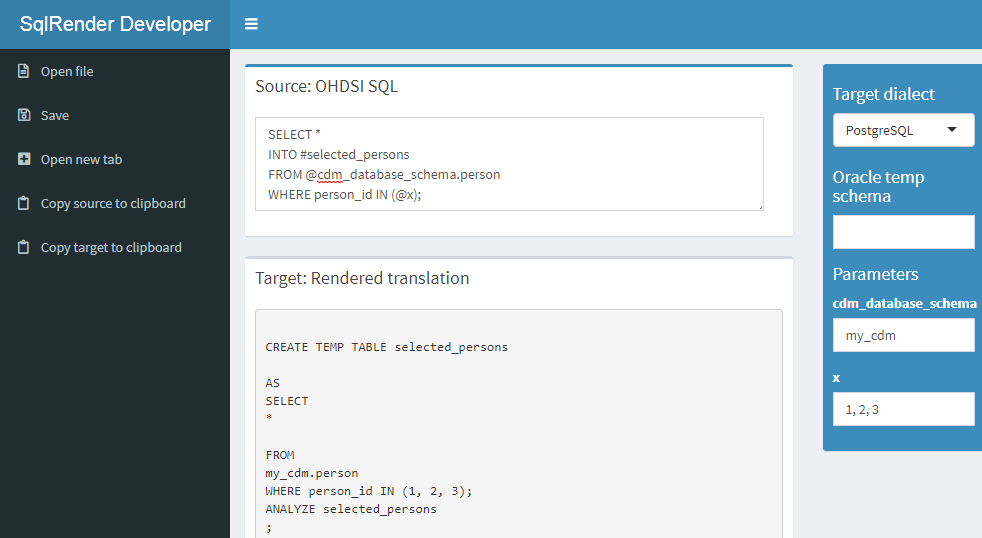
\includegraphics[width=1\linewidth]{images/SqlAndR/sqlDeveloper} 

}

\caption{The SqlDeveloper Shiny app.}\label{fig:sqlDeveloper}
\end{figure}

In the app you can enter OHDSI SQL, select the target dialect as well as
provide values for the parameters that appear in your SQL, and the
translation will automatically appear at the bottom.

\section{DatabaseConnector}\label{DatabaseConnector}

\href{https://ohdsi.github.io/DatabaseConnector/}{DatabaseConnector} is
an R package for connecting to various database platforms using Java's
JDBC drivers. The DatabaseConnector package is available on CRAN (the
Comprehensive R Archive Network), and can therefore be installed using:

\begin{Shaded}
\begin{Highlighting}[]
\KeywordTok{install.packages}\NormalTok{(}\StringTok{"DatabaseConnector"}\NormalTok{)}
\end{Highlighting}
\end{Shaded}

DatabaseConnector supports a wide array of technical platforms including
traditional database systems (PostgreSQL, Microsoft SQL Server, SQLite,
and Oracle), parallel data warehouses (Microsoft APS, IBM Netezza, and
Amazon RedShift), as well as Big Data platforms (Hadoop through Impala,
and Google BigQuery). The package already contains most drivers, but
because of licensing reasons the drivers for BigQuery, Netezza and
Impala are not included but must be obtained by the user. Type
\texttt{?jdbcDrivers} for instructions on how to download these drivers.
Once downloaded, you can use the \texttt{pathToDriver} argument of the
\texttt{connect}, \texttt{dbConnect}, and
\texttt{createConnectionDetails} functions.

\subsection{Creating a Connection}\label{creating-a-connection}

To connect to a database a number of details need to be specified, such
as the database platform, the location of the server, the user name, and
password. We can call the \texttt{connect} function and specify these
details directly: \index{DatabaseConnector!creating a connection}

\begin{Shaded}
\begin{Highlighting}[]
\NormalTok{conn <-}\StringTok{ }\KeywordTok{connect}\NormalTok{(}\DataTypeTok{dbms =} \StringTok{"postgresql"}\NormalTok{,}
                \DataTypeTok{server =} \StringTok{"localhost/postgres"}\NormalTok{,}
                \DataTypeTok{user =} \StringTok{"joe"}\NormalTok{,}
                \DataTypeTok{password =} \StringTok{"secret"}\NormalTok{,}
                \DataTypeTok{schema =} \StringTok{"cdm"}\NormalTok{)}
\end{Highlighting}
\end{Shaded}

\begin{verbatim}
## Connecting using PostgreSQL driver
\end{verbatim}

See \texttt{?connect} for information on which details are required for
each platform. Don't forget to close any connection afterwards:

\begin{Shaded}
\begin{Highlighting}[]
\KeywordTok{disconnect}\NormalTok{(conn)}
\end{Highlighting}
\end{Shaded}

Note that, instead of providing the server name, it is also possible to
provide the JDBC connection string if this is more convenient:

\begin{Shaded}
\begin{Highlighting}[]
\NormalTok{connString <-}\StringTok{ "jdbc:postgresql://localhost:5432/postgres"}
\NormalTok{conn <-}\StringTok{ }\KeywordTok{connect}\NormalTok{(}\DataTypeTok{dbms =} \StringTok{"postgresql"}\NormalTok{,}
                \DataTypeTok{connectionString =}\NormalTok{ connString,}
                \DataTypeTok{user =} \StringTok{"joe"}\NormalTok{,}
                \DataTypeTok{password =} \StringTok{"secret"}\NormalTok{,}
                \DataTypeTok{schema =} \StringTok{"cdm"}\NormalTok{)}
\end{Highlighting}
\end{Shaded}

\begin{verbatim}
## Connecting using PostgreSQL driver
\end{verbatim}

Sometimes we may want to first specify the connection details, and defer
connecting until later. This may be convenient for example when the
connection is established inside a function, and the details need to be
passed as an argument. We can use the \texttt{createConnectionDetails}
function for this purpose:

\begin{Shaded}
\begin{Highlighting}[]
\NormalTok{details <-}\StringTok{ }\KeywordTok{createConnectionDetails}\NormalTok{(}\DataTypeTok{dbms =} \StringTok{"postgresql"}\NormalTok{,}
                                   \DataTypeTok{server =} \StringTok{"localhost/postgres"}\NormalTok{,}
                                   \DataTypeTok{user =} \StringTok{"joe"}\NormalTok{,}
                                   \DataTypeTok{password =} \StringTok{"secret"}\NormalTok{,}
                                   \DataTypeTok{schema =} \StringTok{"cdm"}\NormalTok{)}
\NormalTok{conn <-}\StringTok{ }\KeywordTok{connect}\NormalTok{(details)}
\end{Highlighting}
\end{Shaded}

\begin{verbatim}
## Connecting using PostgreSQL driver
\end{verbatim}

\subsection{Querying}\label{querying}

The main functions for querying database are the \texttt{querySql} and
\texttt{executeSql} functions. The difference between these functions is
that \texttt{querySql} expects data to be returned by the database, and
can handle only one SQL statement at a time. In contrast,
\texttt{executeSql} does not expect data to be returned, and accepts
multiple SQL statements in a single SQL string.
\index{DatabaseConnector!querying}

Some examples:

\begin{Shaded}
\begin{Highlighting}[]
\KeywordTok{querySql}\NormalTok{(conn, }\StringTok{"SELECT TOP 3 * FROM person"}\NormalTok{)}
\end{Highlighting}
\end{Shaded}

\begin{verbatim}
##   person_id gender_concept_id year_of_birth
## 1         1              8507          1975
## 2         2              8507          1976
## 3         3              8507          1977
\end{verbatim}

\begin{Shaded}
\begin{Highlighting}[]
\KeywordTok{executeSql}\NormalTok{(conn, }\StringTok{"TRUNCATE TABLE foo; DROP TABLE foo;"}\NormalTok{)}
\end{Highlighting}
\end{Shaded}

Both functions provide extensive error reporting: When an error is
thrown by the server, the error message and the offending piece of SQL
are written to a text file to allow better debugging. The
\texttt{executeSql} function also by default shows a progress bar,
indicating the percentage of SQL statements that has been executed. If
those attributes are not desired, the package also offers the
\texttt{lowLevelQuerySql} and \texttt{lowLevelExecuteSql} functions.

\subsection{Querying Using Ffdf
Objects}\label{querying-using-ffdf-objects}

Sometimes the data to be fetched from the database is too large to fit
into memory. As mentioned in Section \ref{BigDataSupport}, in such a
case we can use the \texttt{ff} package to store R data objects on file,
and use them as if they are available in memory.
\texttt{DatabaseConnector} can download data directly into ffdf objects:

\begin{Shaded}
\begin{Highlighting}[]
\NormalTok{x <-}\StringTok{ }\KeywordTok{querySql.ffdf}\NormalTok{(conn, }\StringTok{"SELECT * FROM person"}\NormalTok{)}
\end{Highlighting}
\end{Shaded}

x is now an ffdf object.

\subsection{Querying Different Platforms Using the Same
SQL}\label{querying-different-platforms-using-the-same-sql}

The following convenience functions are available that first call the
\texttt{render} and \texttt{translate} functions in the SqlRender
package: \texttt{renderTranslateExecuteSql},
\texttt{renderTranslateQuerySql}, \texttt{renderTranslateQuerySql.ffdf}.
For example:

\begin{Shaded}
\begin{Highlighting}[]
\NormalTok{x <-}\StringTok{ }\KeywordTok{renderTranslateQuerySql}\NormalTok{(conn, }
                             \DataTypeTok{sql =} \StringTok{"SELECT TOP 10 * FROM @schema.person"}\NormalTok{,}
                             \DataTypeTok{schema =} \StringTok{"cdm_synpuf"}\NormalTok{)}
\end{Highlighting}
\end{Shaded}

Note that the SQL Server-specific `TOP 10' syntax will be translated to
for example `LIMIT 10' on PostgreSQL, and that the SQL parameter
\texttt{@schema} will be instantiated with the provided value
`cdm\_synpuf'.

\subsection{Inserting Tables}\label{inserting-tables}

Although it is also possible to insert data in the database by sending
SQL statements using the \texttt{executeSql} function, it is often more
convenient and faster (due to some optimization) to use the
\texttt{insertTable} function:

\begin{Shaded}
\begin{Highlighting}[]
\KeywordTok{data}\NormalTok{(mtcars)}
\KeywordTok{insertTable}\NormalTok{(conn, }\StringTok{"mtcars"}\NormalTok{, mtcars, }\DataTypeTok{createTable =} \OtherTok{TRUE}\NormalTok{)}
\end{Highlighting}
\end{Shaded}

In this example, we're uploading the mtcars data frame to a table called
`mtcars' on the server, which will be automatically created.

\section{Querying the CDM}\label{QueryTheCdm}

In the following examples we use OHDSI SQL to query a database that
adheres to the CDM. These queries use \texttt{@cdm} to denote the
database schema where the data in CDM can be found.

We can start by just querying how many people are in the database:

\begin{Shaded}
\begin{Highlighting}[]
\KeywordTok{SELECT} \FunctionTok{COUNT}\NormalTok{(*) }\KeywordTok{AS}\NormalTok{ person_count }\KeywordTok{FROM}\NormalTok{ @cdm.person;}
\end{Highlighting}
\end{Shaded}

\begin{longtable}[]{@{}r@{}}
\toprule
PERSON\_COUNT\tabularnewline
\midrule
\endhead
26299001\tabularnewline
\bottomrule
\end{longtable}

Or perhaps we're interested in the average length of an observation
period:

\begin{Shaded}
\begin{Highlighting}[]
\KeywordTok{SELECT} \FunctionTok{AVG}\NormalTok{(DATEDIFF(}\DataTypeTok{DAY}\NormalTok{, }
\NormalTok{                    observation_period_start_date, }
\NormalTok{                    observation_period_end_date) / }\FloatTok{365.25}\NormalTok{) }\KeywordTok{AS}\NormalTok{ num_years}
\KeywordTok{FROM}\NormalTok{ @cdm.observation_period;}
\end{Highlighting}
\end{Shaded}

\begin{longtable}[]{@{}r@{}}
\toprule
NUM\_YEARS\tabularnewline
\midrule
\endhead
1.980803\tabularnewline
\bottomrule
\end{longtable}

We can join tables to produce additional statistics. A join combines
fields from multiple tables, typically by requiring specific fields in
the tables to have the same value. For example, here we join the PERSON
table to the OBSERVATION\_PERIOD table on the PERSON\_ID fields in both
tables. In other words, the result of the join is a new table-like set
that has all the fields of the two tables, but in all rows the
PERSON\_ID fields from the two tables must have the same value. We can
now for example compute the maximum age at observation end by using the
OBSERVATION\_PERIOD\_END\_DATE field from the OBSERVATION\_PERIOD table
together with the year\_of\_birth field of the PERSON table:

\begin{Shaded}
\begin{Highlighting}[]
\KeywordTok{SELECT} \FunctionTok{MAX}\NormalTok{(}\DataTypeTok{YEAR}\NormalTok{(observation_period_end_date) -}
\NormalTok{           year_of_birth) }\KeywordTok{AS}\NormalTok{ max_age}
\KeywordTok{FROM}\NormalTok{ @cdm.person}
\KeywordTok{INNER} \KeywordTok{JOIN}\NormalTok{ @cdm.observation_period}
  \KeywordTok{ON}\NormalTok{ person.person_id = observation_period.person_id;}
\end{Highlighting}
\end{Shaded}

\begin{longtable}[]{@{}r@{}}
\toprule
MAX\_AGE\tabularnewline
\midrule
\endhead
90\tabularnewline
\bottomrule
\end{longtable}

A much more complicated query is needed to determine the distribution of
age at the start of observation. In this query, we first join the PERSON
to the OBSERVATION\_PERIOD table to compute age at start of observation.
We also compute the ordering for this joined set based on age, and store
it as order\_nr. Because we want to use the result of this join multiple
times, we define it as a common table expression (CTE) (defined using
\texttt{WITH\ ...\ AS}) that we call ``ages,'' meaning we can refer to
ages as if it is an existing table. We count the number of rows in ages
to produce ``n,'' and then for each quantile find the minimum age where
the order\_nr is smaller than the fraction times n. For example, to find
the median we use the minimum age where \(order\_nr < .50 * n\). The
minimum and maximum age are computed separately:

\begin{Shaded}
\begin{Highlighting}[]
\KeywordTok{WITH}\NormalTok{ ages}
\KeywordTok{AS}\NormalTok{ (}
    \KeywordTok{SELECT}\NormalTok{ age,}
        \FunctionTok{ROW_NUMBER}\NormalTok{() }\KeywordTok{OVER}\NormalTok{ (}
            \KeywordTok{ORDER} \KeywordTok{BY}\NormalTok{ age}
\NormalTok{            ) order_nr}
    \KeywordTok{FROM}\NormalTok{ (}
        \KeywordTok{SELECT} \DataTypeTok{YEAR}\NormalTok{(observation_period_start_date) - year_of_birth }\KeywordTok{AS}\NormalTok{ age}
        \KeywordTok{FROM}\NormalTok{ @cdm.person}
        \KeywordTok{INNER} \KeywordTok{JOIN}\NormalTok{ @cdm.observation_period}
            \KeywordTok{ON}\NormalTok{ person.person_id = observation_period.person_id}
\NormalTok{        ) age_computed}
\NormalTok{    )}
\KeywordTok{SELECT} \FunctionTok{MIN}\NormalTok{(age) }\KeywordTok{AS}\NormalTok{ min_age,}
    \FunctionTok{MIN}\NormalTok{(}\KeywordTok{CASE} 
            \KeywordTok{WHEN}\NormalTok{ order_nr < .}\DecValTok{25}\NormalTok{ * n}
                \KeywordTok{THEN} \DecValTok{9999}
            \KeywordTok{ELSE}\NormalTok{ age}
            \KeywordTok{END}\NormalTok{) }\KeywordTok{AS}\NormalTok{ q25_age,}
    \FunctionTok{MIN}\NormalTok{(}\KeywordTok{CASE} 
            \KeywordTok{WHEN}\NormalTok{ order_nr < .}\DecValTok{50}\NormalTok{ * n}
                \KeywordTok{THEN} \DecValTok{9999}
            \KeywordTok{ELSE}\NormalTok{ age}
            \KeywordTok{END}\NormalTok{) }\KeywordTok{AS}\NormalTok{ median_age,}
    \FunctionTok{MIN}\NormalTok{(}\KeywordTok{CASE} 
            \KeywordTok{WHEN}\NormalTok{ order_nr < .}\DecValTok{75}\NormalTok{ * n}
                \KeywordTok{THEN} \DecValTok{9999}
            \KeywordTok{ELSE}\NormalTok{ age}
            \KeywordTok{END}\NormalTok{) }\KeywordTok{AS}\NormalTok{ q75_age,}
    \FunctionTok{MAX}\NormalTok{(age) }\KeywordTok{AS}\NormalTok{ max_age}
\KeywordTok{FROM}\NormalTok{ ages}
\KeywordTok{CROSS} \KeywordTok{JOIN}\NormalTok{ (}
    \KeywordTok{SELECT} \FunctionTok{COUNT}\NormalTok{(*) }\KeywordTok{AS}\NormalTok{ n}
    \KeywordTok{FROM}\NormalTok{ ages}
\NormalTok{    ) population_size;}
\end{Highlighting}
\end{Shaded}

\begin{longtable}[]{@{}rrrrr@{}}
\toprule
MIN\_AGE & Q25\_AGE & MEDIAN\_AGE & Q75\_AGE & MAX\_AGE\tabularnewline
\midrule
\endhead
0 & 6 & 17 & 34 & 90\tabularnewline
\bottomrule
\end{longtable}

More complex computations can also be performed in R instead of using
SQL. For example, we can get the same answer using this R code:

\begin{Shaded}
\begin{Highlighting}[]
\NormalTok{sql <-}\StringTok{ "SELECT YEAR(observation_period_start_date) -}
\StringTok{               year_of_birth AS age}
\StringTok{FROM @cdm.person}
\StringTok{INNER JOIN @cdm.observation_period}
\StringTok{  ON person.person_id = observation_period.person_id;"}
\NormalTok{age <-}\StringTok{ }\KeywordTok{renderTranslateQuerySql}\NormalTok{(conn, sql, }\DataTypeTok{cdm =} \StringTok{"cdm"}\NormalTok{)}
\KeywordTok{quantile}\NormalTok{(age[, }\DecValTok{1}\NormalTok{], }\KeywordTok{c}\NormalTok{(}\DecValTok{0}\NormalTok{, }\FloatTok{0.25}\NormalTok{, }\FloatTok{0.5}\NormalTok{, }\FloatTok{0.75}\NormalTok{, }\DecValTok{1}\NormalTok{))}
\end{Highlighting}
\end{Shaded}

\begin{verbatim}
##   0%  25%  50%  75% 100% 
##    0    6   17   34   90
\end{verbatim}

Here we compute age on the server, download all ages, and then compute
the age distribution. However, this requires millions of rows of data to
be downloaded from the database server, and is therefore not very
efficient. You will need to decide on a case-by-case basis whether a
computation is best performed in SQL or in R.

Queries can use the source values in the CDM. For example, we can
retrieve the top 10 most frequent condition source codes using:

\begin{Shaded}
\begin{Highlighting}[]
\KeywordTok{SELECT}\NormalTok{ TOP }\DecValTok{10}\NormalTok{ condition_source_value, }
  \FunctionTok{COUNT}\NormalTok{(*) }\KeywordTok{AS}\NormalTok{ code_count}
\KeywordTok{FROM}\NormalTok{ @cdm.condition_occurrence}
\KeywordTok{GROUP} \KeywordTok{BY}\NormalTok{ condition_source_value}
\KeywordTok{ORDER} \KeywordTok{BY}\NormalTok{ -COUNT(*);}
\end{Highlighting}
\end{Shaded}

\begin{longtable}[]{@{}rr@{}}
\toprule
CONDITION\_SOURCE\_VALUE & CODE\_COUNT\tabularnewline
\midrule
\endhead
4019 & 49094668\tabularnewline
25000 & 36149139\tabularnewline
78099 & 28908399\tabularnewline
319 & 25798284\tabularnewline
31401 & 22547122\tabularnewline
317 & 22453999\tabularnewline
311 & 19626574\tabularnewline
496 & 19570098\tabularnewline
I10 & 19453451\tabularnewline
3180 & 18973883\tabularnewline
\bottomrule
\end{longtable}

Here we grouped records in the CONDITION\_OCCURRENCE table by values of
the CONDITION\_SOURCE\_VALUE field, and counted the number of records in
each group. We retrieve the CONDITION\_SOURCE\_VALUE and the count, and
reverse-order it by the count.

\section{Using the Vocabulary When
Querying}\label{using-the-vocabulary-when-querying}

Many operations require the vocabulary to be useful. The Vocabulary
tables are part of the CDM, and are therefore available using SQL
queries. Here we show how queries against the Vocabulary can be combined
with queries against the CDM. Many fields in the CDM contain concept IDs
which can be resolved using the CONCEPT table. For example, we may wish
to count the number of persons in the database stratified by gender, and
it would be convenient to resolve the GENDER\_CONCEPT\_ID field to a
concept name:

\begin{Shaded}
\begin{Highlighting}[]
\KeywordTok{SELECT} \FunctionTok{COUNT}\NormalTok{(*) }\KeywordTok{AS}\NormalTok{ subject_count,}
\NormalTok{  concept_name}
\KeywordTok{FROM}\NormalTok{ @cdm.person}
\KeywordTok{INNER} \KeywordTok{JOIN}\NormalTok{ @cdm.concept}
  \KeywordTok{ON}\NormalTok{ person.gender_concept_id = concept.concept_id}
\KeywordTok{GROUP} \KeywordTok{BY}\NormalTok{ concept_name;}
\end{Highlighting}
\end{Shaded}

\begin{longtable}[]{@{}rr@{}}
\toprule
SUBJECT\_COUNT & CONCEPT\_NAME\tabularnewline
\midrule
\endhead
14927548 & FEMALE\tabularnewline
11371453 & MALE\tabularnewline
\bottomrule
\end{longtable}

A very powerful feature of the Vocabulary is its hierarchy. A very
common query looks for a specific concept \emph{and all of its
descendants}. For example, imagine we wish to count the number of
prescriptions containing the ingredient ibuprofen:

\begin{Shaded}
\begin{Highlighting}[]
\KeywordTok{SELECT} \FunctionTok{COUNT}\NormalTok{(*) }\KeywordTok{AS}\NormalTok{ prescription_count}
\KeywordTok{FROM}\NormalTok{ @cdm.drug_exposure}
\KeywordTok{INNER} \KeywordTok{JOIN}\NormalTok{ @cdm.concept_ancestor}
  \KeywordTok{ON}\NormalTok{ drug_concept_id = descendant_concept_id}
\KeywordTok{INNER} \KeywordTok{JOIN}\NormalTok{ @cdm.concept ingredient}
  \KeywordTok{ON}\NormalTok{ ancestor_concept_id = ingredient.concept_id}
\KeywordTok{WHERE} \FunctionTok{LOWER}\NormalTok{(ingredient.concept_name) = }\StringTok{'ibuprofen'}
  \KeywordTok{AND}\NormalTok{ ingredient.concept_class_id = }\StringTok{'Ingredient'}
  \KeywordTok{AND}\NormalTok{ ingredient.standard_concept = }\StringTok{'S'}\NormalTok{;}
\end{Highlighting}
\end{Shaded}

\begin{longtable}[]{@{}r@{}}
\toprule
PRESCRIPTION\_COUNT\tabularnewline
\midrule
\endhead
26871214\tabularnewline
\bottomrule
\end{longtable}

\section{QueryLibrary}\label{querylibrary}

\index{QueryLibrary}

QueryLibrary is a library of commonly-used SQL queries for the CDM. It
is available as an online application\footnote{\url{http://data.ohdsi.org/QueryLibrary}}
shown in Figure \ref{fig:queryLibrary}, and as an R package.\footnote{\url{https://github.com/OHDSI/QueryLibrary}}

\begin{figure}

{\centering 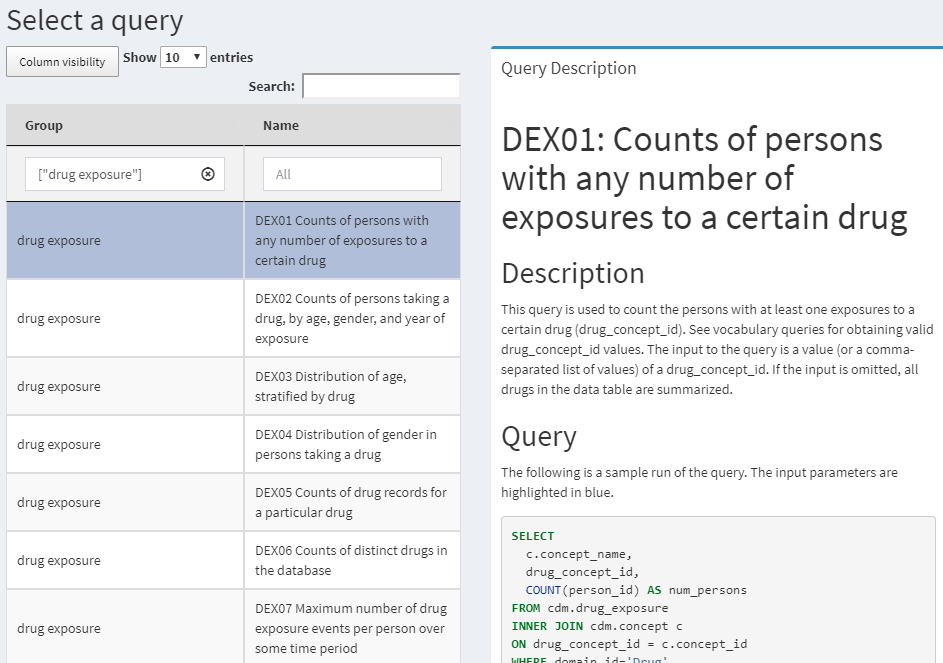
\includegraphics[width=1\linewidth]{images/SqlAndR/queryLibrary} 

}

\caption{QueryLibrary: a library of SQL queries against the CDM.}\label{fig:queryLibrary}
\end{figure}

The purpose of the library is to help new users learn how to query the
CDM. The queries in the library have been reviewed and approved by the
OHDSI community. The query library is primarily intended for training
purposes, but it is also a valuable resource for experienced users.

The QueryLibrary makes use of SqlRender to output the queries in the SQL
dialect of choice. Users can also specify the CDM database schema,
vocabulary database schema (if separate), and the Oracle temp schema (if
needed), so the queries will be automatically rendered with these
settings.

\section{Designing a Simple Study}\label{designing-a-simple-study}

\subsection{Problem Definition}\label{problem-definition}

Angioedema is a well-known side-effect of ACE inhibitors (ACEi).
\citet{slater_1988} estimate the incidence rate of angioedema in the
first week of ACEi treatment to be one case per 3,000 patients per week.
Here we seek to replicate this finding, and stratify by age and gender.
For simplicity, we focus on one ACEi: lisinopril. We thus answer the
question

\begin{quote}
What is the rate of angioedema in the first week following lisinopril
treatment initiation, stratified by age and gender?
\end{quote}

\subsection{Exposure}\label{exposure}

We'll define exposure as first exposure to lisinopril. By first we mean
no earlier exposure to lisinopril. We require 365 days of continuous
observation time prior to the first exposure.

\subsection{Outcome}\label{outcome}

We define angioedema as any occurrence of an angioedema diagnosis code
during an inpatient or emergency room (ER) visit.

\subsection{Time-At-Risk}\label{time-at-risk}

We will compute the incidence rate in the first week following treatment
initiation, irrespective of whether patients were exposed for the full
week.

\section{Implementing the Study Using SQL and
R}\label{implementing-the-study-using-sql-and-r}

Although we are not bound to any of the OHDSI tool conventions, it is
helpful to follow the same principles. In this case, we will use SQL to
populate a cohort table, similarly to how the OHDSI tools work. The
COHORT table is defined in the CDM, and has a predefined set of fields
that we will also use. We first must create the COHORT table in a
database schema where we have write access, which likely is not the same
as the database schema that holds the data in CDM format.

\begin{Shaded}
\begin{Highlighting}[]
\KeywordTok{library}\NormalTok{(DatabaseConnector)}
\NormalTok{conn <-}\StringTok{ }\KeywordTok{connect}\NormalTok{(}\DataTypeTok{dbms =} \StringTok{"postgresql"}\NormalTok{,}
                \DataTypeTok{server =} \StringTok{"localhost/postgres"}\NormalTok{,}
                \DataTypeTok{user =} \StringTok{"joe"}\NormalTok{,}
                \DataTypeTok{password =} \StringTok{"secret"}\NormalTok{)}
\NormalTok{cdmDbSchema <-}\StringTok{ "cdm"}
\NormalTok{cohortDbSchema <-}\StringTok{ "scratch"}
\NormalTok{cohortTable <-}\StringTok{ "my_cohorts"}

\NormalTok{sql <-}\StringTok{ "}
\StringTok{CREATE TABLE @cohort_db_schema.@cohort_table (}
\StringTok{  cohort_definition_id INT,}
\StringTok{  cohort_start_date DATE,}
\StringTok{  cohort_end_date DATE,}
\StringTok{  subject_id BIGINT}
\StringTok{);}
\StringTok{"}
\KeywordTok{renderTranslateExecuteSql}\NormalTok{(conn, sql,}
                          \DataTypeTok{cohort_db_schema =}\NormalTok{ cohortDbSchema,}
                          \DataTypeTok{cohort_table =}\NormalTok{ cohortTable)}
\end{Highlighting}
\end{Shaded}

Here we have parameterized the database schema and table names, so we
can easily adapt them to different environments. The result is an empty
table on the database server.

\subsection{Exposure Cohort}\label{exposure-cohort}

Next we create our exposure cohort, and insert it into our COHORT table:

\begin{Shaded}
\begin{Highlighting}[]
\NormalTok{sql <-}\StringTok{ "}
\StringTok{INSERT INTO @cohort_db_schema.@cohort_table (}
\StringTok{  cohort_definition_id,}
\StringTok{  cohort_start_date,}
\StringTok{  cohort_end_date,}
\StringTok{  subject_id}
\StringTok{)}
\StringTok{SELECT 1 AS cohort_definition_id,}
\StringTok{  cohort_start_date,}
\StringTok{  cohort_end_date,}
\StringTok{  subject_id}
\StringTok{FROM (}
\StringTok{  SELECT drug_era_start_date AS cohort_start_date,}
\StringTok{    drug_era_end_date AS cohort_end_date,}
\StringTok{    person_id AS subject_id}
\StringTok{  FROM (}
\StringTok{    SELECT drug_era_start_date,}
\StringTok{      drug_era_end_date,}
\StringTok{      person_id,}
\StringTok{      ROW_NUMBER() OVER (}
\StringTok{        PARTITION BY person_id}
\StringTok{            ORDER BY drug_era_start_date}
\StringTok{      ) order_nr}
\StringTok{    FROM @cdm_db_schema.drug_era}
\StringTok{    WHERE drug_concept_id = 1308216 -- Lisinopril}
\StringTok{  ) ordered_exposures}
\StringTok{  WHERE order_nr = 1}
\StringTok{) first_era}
\StringTok{INNER JOIN @cdm_db_schema.observation_period}
\StringTok{  ON subject_id = person_id}
\StringTok{    AND observation_period_start_date < cohort_start_date}
\StringTok{    AND observation_period_end_date > cohort_start_date}
\StringTok{WHERE DATEDIFF(DAY,}
\StringTok{               observation_period_start_date,}
\StringTok{               cohort_start_date) >= 365;}
\StringTok{"}

\KeywordTok{renderTranslateExecuteSql}\NormalTok{(conn, sql,}
                          \DataTypeTok{cohort_db_schema =}\NormalTok{ cohortDbSchema,}
                          \DataTypeTok{cohort_table =}\NormalTok{ cohortTable,}
                          \DataTypeTok{cdm_db_schema =}\NormalTok{ cdmDbSchema)}
\end{Highlighting}
\end{Shaded}

Here we use the DRUG\_ERA table, a standard table in the CDM that is
automatically derived from the DRUG\_EXPOSURE table. The DRUG\_ERA table
contains eras of continuous exposure at the ingredient level. We can
thus search for lisinopril, and this will automatically identify all
exposures to drugs containing lisinopril. We take the first drug
exposure per person, and then join to the OBSERVATION\_PERIOD table, and
because a person can have several observation periods we must make sure
we only join to the period containing the drug exposure. We then require
at least 365 days between the OBSERVATION\_PERIOD\_START\_DATE and the
COHORT\_START\_DATE.

\subsection{Outcome Cohort}\label{outcome-cohort}

Finally, we must create our outcome cohort:

\begin{Shaded}
\begin{Highlighting}[]
\NormalTok{sql <-}\StringTok{ "}
\StringTok{INSERT INTO @cohort_db_schema.@cohort_table (}
\StringTok{ cohort_definition_id,}
\StringTok{ cohort_start_date,}
\StringTok{ cohort_end_date,}
\StringTok{subject_id}
\StringTok{)}
\StringTok{SELECT 2 AS cohort_definition_id,}
\StringTok{  cohort_start_date,}
\StringTok{  cohort_end_date,}
\StringTok{  subject_id}
\StringTok{FROM (}
\StringTok{  SELECT DISTINCT person_id AS subject_id,}
\StringTok{    condition_start_date AS cohort_start_date,}
\StringTok{    condition_end_date AS cohort_end_date}
\StringTok{  FROM @cdm_db_schema.condition_occurrence}
\StringTok{  INNER JOIN @cdm_db_schema.concept_ancestor}
\StringTok{    ON condition_concept_id = descendant_concept_id}
\StringTok{  WHERE ancestor_concept_id = 432791 -- Angioedema}
\StringTok{) distinct_occurrence}
\StringTok{INNER JOIN @cdm_db_schema.visit_occurrence}
\StringTok{  ON subject_id = person_id}
\StringTok{  AND visit_start_date <= cohort_start_date}
\StringTok{  AND visit_end_date >= cohort_start_date}
\StringTok{WHERE visit_concept_id IN (262, 9203,}
\StringTok{    9201) -- Inpatient or ER;}
\StringTok{"}

\KeywordTok{renderTranslateExecuteSql}\NormalTok{(conn, sql,}
                          \DataTypeTok{cohort_db_schema =}\NormalTok{ cohortDbSchema,}
                          \DataTypeTok{cohort_table =}\NormalTok{ cohortTable,}
                          \DataTypeTok{cdm_db_schema =}\NormalTok{ cdmDbSchema)}
\end{Highlighting}
\end{Shaded}

Here we join the CONDITION\_OCCURRENCE table to the CONCEPT\_ANCESTOR
table to find all occurrences of angioedema or any of its descendants.
We use DISTINCT to make sure we only select one record per day, as we
believe multiple angioedema diagnoses on the same day are more likely to
be the same occurrence rather than multiple angioedema events. We join
these occurrences to the VISIT\_OCCURRENCE table to ensure the diagnosis
was made in and inpatient or ER setting.

\subsection{Incidence Rate
Calculation}\label{incidence-rate-calculation}

Now that our cohorts are in place, we can compute the incidence rate,
stratified by age and gender:

\begin{Shaded}
\begin{Highlighting}[]
\NormalTok{sql <-}\StringTok{ "}
\StringTok{WITH tar AS (}
\StringTok{  SELECT concept_name AS gender,}
\StringTok{    FLOOR((YEAR(cohort_start_date) -}
\StringTok{          year_of_birth) / 10) AS age,}
\StringTok{    subject_id,}
\StringTok{    cohort_start_date,}
\StringTok{    CASE WHEN DATEADD(DAY, 7, cohort_start_date) >}
\StringTok{      observation_period_end_date}
\StringTok{    THEN observation_period_end_date}
\StringTok{    ELSE DATEADD(DAY, 7, cohort_start_date)}
\StringTok{    END AS cohort_end_date}
\StringTok{  FROM @cohort_db_schema.@cohort_table}
\StringTok{  INNER JOIN @cdm_db_schema.observation_period}
\StringTok{    ON subject_id = observation_period.person_id}
\StringTok{      AND observation_period_start_date < cohort_start_date}
\StringTok{      AND observation_period_end_date > cohort_start_date}
\StringTok{  INNER JOIN @cdm_db_schema.person}
\StringTok{    ON subject_id = person.person_id}
\StringTok{  INNER JOIN @cdm_db_schema.concept}
\StringTok{    ON gender_concept_id = concept_id}
\StringTok{  WHERE cohort_definition_id = 1 -- Exposure}
\StringTok{)}
\StringTok{SELECT days.gender,}
\StringTok{    days.age,}
\StringTok{    days,}
\StringTok{    CASE WHEN events IS NULL THEN 0 ELSE events END AS events}
\StringTok{FROM (}
\StringTok{  SELECT gender,}
\StringTok{    age,}
\StringTok{    SUM(DATEDIFF(DAY, cohort_start_date,}
\StringTok{      cohort_end_date)) AS days}
\StringTok{  FROM tar}
\StringTok{  GROUP BY gender,}
\StringTok{    age}
\StringTok{) days}
\StringTok{LEFT JOIN (}
\StringTok{  SELECT gender,}
\StringTok{      age,}
\StringTok{      COUNT(*) AS events}
\StringTok{  FROM tar}
\StringTok{  INNER JOIN @cohort_db_schema.@cohort_table angioedema}
\StringTok{    ON tar.subject_id = angioedema.subject_id}
\StringTok{      AND tar.cohort_start_date <= angioedema.cohort_start_date}
\StringTok{      AND tar.cohort_end_date >= angioedema.cohort_start_date}
\StringTok{  WHERE cohort_definition_id = 2 -- Outcome}
\StringTok{  GROUP BY gender,}
\StringTok{    age}
\StringTok{) events}
\StringTok{ON days.gender = events.gender}
\StringTok{  AND days.age = events.age;}
\StringTok{"}

\NormalTok{results <-}\StringTok{ }\KeywordTok{renderTranslateQuerySql}\NormalTok{(conn, sql,}
                                   \DataTypeTok{cohort_db_schema =}\NormalTok{ cohortDbSchema,}
                                   \DataTypeTok{cohort_table =}\NormalTok{ cohortTable,}
                                   \DataTypeTok{cdm_db_schema =}\NormalTok{ cdmDbSchema,}
                                   \DataTypeTok{snakeCaseToCamelCase =} \OtherTok{TRUE}\NormalTok{)}
\end{Highlighting}
\end{Shaded}

We first create ``tar,'' a CTE that contains all exposures with the
appropriate time-at-risk. Note that we truncate the time-at-risk at the
OBSERVATION\_PERIOD\_END\_DATE. We also compute the age in 10-year bins,
and identify the gender. The advantage of using a CTE is that we can use
the same set of intermediate results several times in a query. In this
case we use it to count the total amount of time-at-risk, as well as the
number of angioedema events that occur during the time-at-risk.

We use \texttt{snakeCaseToCamelCase\ =\ TRUE} because in SQL we tend to
use snake\_case for field names (because SQL in case-insensitive),
whereas in R we tend to use camelCase (because R is case-sensitive). The
\texttt{results} data frame column names will now be in camelCase.

With the help of the ggplot2 package we can easily plot our results:

\begin{Shaded}
\begin{Highlighting}[]
\CommentTok{# Compute incidence rate (IR) :}
\NormalTok{results}\OperatorTok{$}\NormalTok{ir <-}\StringTok{ }\DecValTok{1000} \OperatorTok{*}\StringTok{ }\NormalTok{results}\OperatorTok{$}\NormalTok{events }\OperatorTok{/}\StringTok{ }\NormalTok{results}\OperatorTok{$}\NormalTok{days }\OperatorTok{/}\StringTok{ }\DecValTok{7}

\CommentTok{# Fix age scale:}
\NormalTok{results}\OperatorTok{$}\NormalTok{age <-}\StringTok{ }\NormalTok{results}\OperatorTok{$}\NormalTok{age }\OperatorTok{*}\StringTok{ }\DecValTok{10}

\KeywordTok{library}\NormalTok{(ggplot2)}
\KeywordTok{ggplot}\NormalTok{(results, }\KeywordTok{aes}\NormalTok{(}\DataTypeTok{x =}\NormalTok{ age, }\DataTypeTok{y =}\NormalTok{ ir, }\DataTypeTok{group =}\NormalTok{ gender, }\DataTypeTok{color =}\NormalTok{ gender)) }\OperatorTok{+}
\StringTok{  }\KeywordTok{geom_line}\NormalTok{() }\OperatorTok{+}
\StringTok{  }\KeywordTok{xlab}\NormalTok{(}\StringTok{"Age"}\NormalTok{) }\OperatorTok{+}
\StringTok{  }\KeywordTok{ylab}\NormalTok{(}\StringTok{"Incidence (per 1,000 patient weeks)"}\NormalTok{)}
\end{Highlighting}
\end{Shaded}

\begin{center}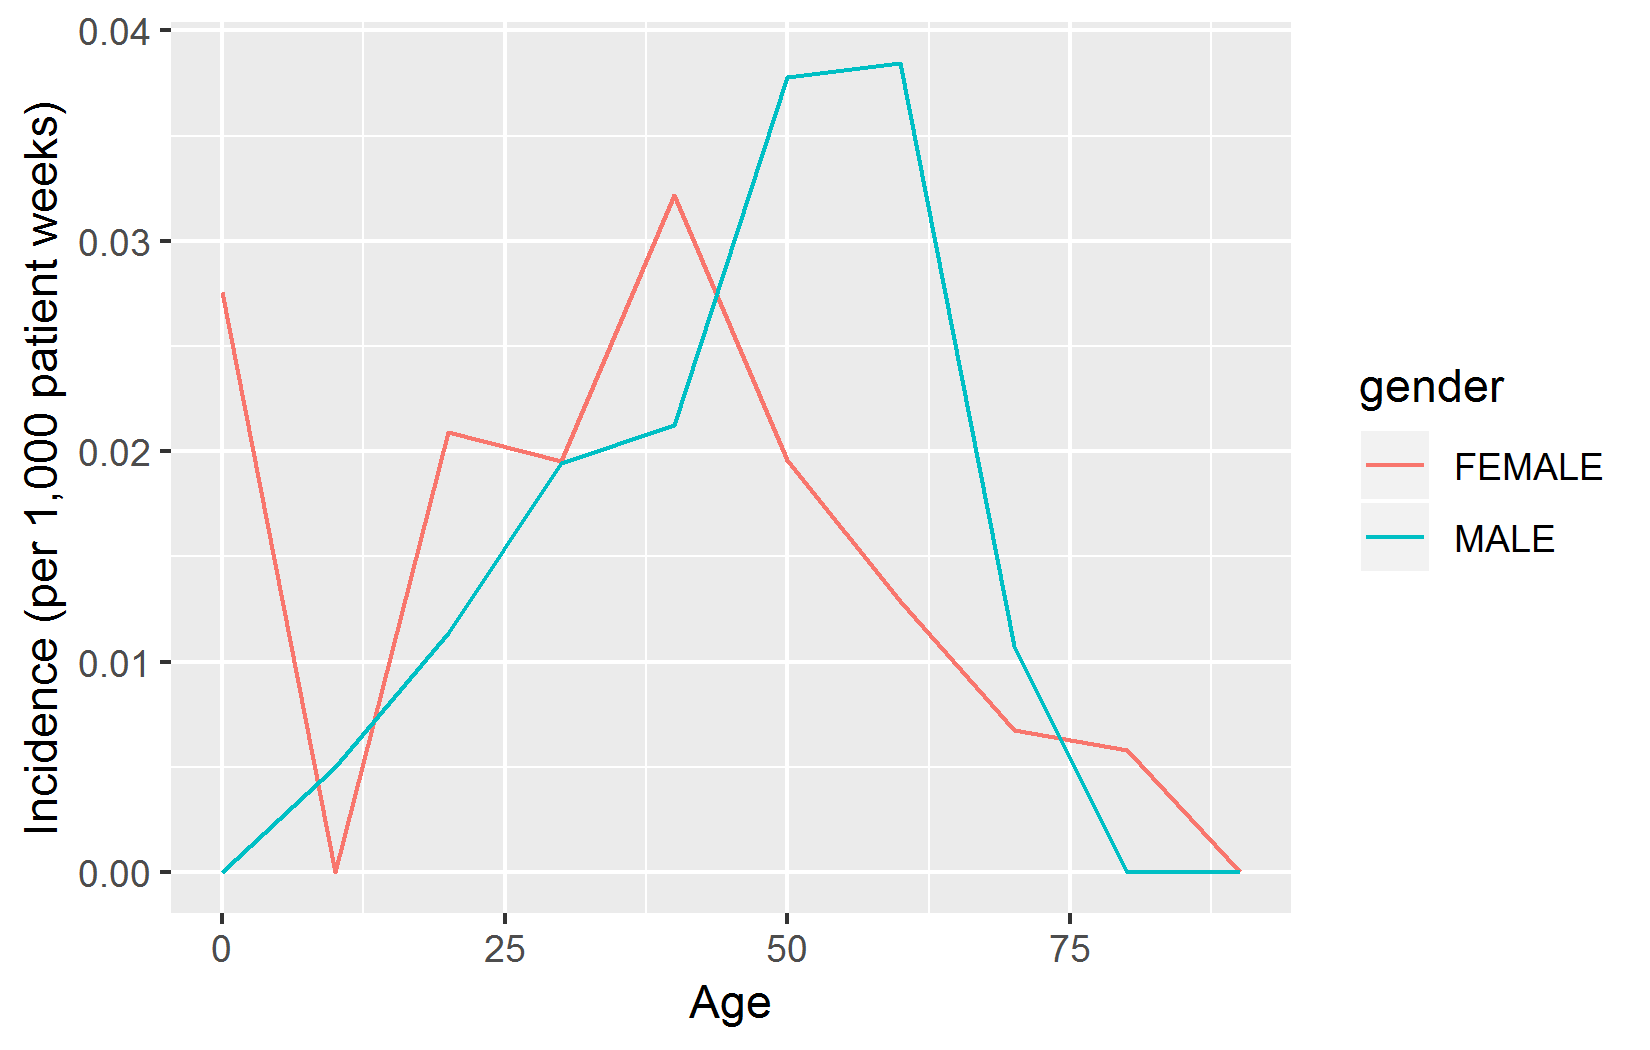
\includegraphics[width=0.8\linewidth]{images/SqlAndR/ir} \end{center}

\subsection{Clean Up}\label{clean-up}

Don't forget to clean up the table we created, and to close the
connection:

\begin{Shaded}
\begin{Highlighting}[]
\NormalTok{sql <-}\StringTok{ "}
\StringTok{TRUNCATE TABLE @cohort_db_schema.@cohort_table;}
\StringTok{DROP TABLE @cohort_db_schema.@cohort_table;}
\StringTok{"}
\KeywordTok{renderTranslateExecuteSql}\NormalTok{(conn, sql,}
                          \DataTypeTok{cohort_db_schema =}\NormalTok{ cohortDbSchema,}
                          \DataTypeTok{cohort_table =}\NormalTok{ cohortTable)}

\KeywordTok{disconnect}\NormalTok{(conn)}
\end{Highlighting}
\end{Shaded}

\subsection{Compatibility}\label{compatibility}

Because we use OHDSI SQL together with DatabaseConnector and SqlRender
throughout, the code we reviewed here will run on any database platform
supported by OHDSI.

Note that for demonstration purposes we chose to create our cohorts
using hand-crafted SQL. It would probably have been more convenient to
construct cohort definition in ATLAS, and use the SQL generated by ATLAS
to instantiate the cohorts. ATLAS also produced OHDSI SQL, and can
therefore easily be used together with SqlRender and DatabaseConnector.

\section{Summary}\label{summary-7}

\BeginKnitrBlock{rmdsummary}
\begin{itemize}
\item
  \textbf{SQL} (Structured Query Language) is a standard language for
  querying databases, including those that conform to the Common Data
  Model (CDM).
\item
  Different database platforms have different SQL dialects, and require
  different tools to query them.
\item
  The \textbf{SqlRender} and \textbf{DatabaseConnector} R packages
  provide a unified way to query data in the CDM, allowing the same
  analysis code to be run in different environments without
  modification.
\item
  By using R and SQL together we can implement custom analyses that are
  not supported by the OHDSI tools.
\item
  The \textbf{QueryLibrary} provides a collection of re-usable SQL
  queries for the CDM.
\end{itemize}
\EndKnitrBlock{rmdsummary}

\section{Exercises}\label{exercises-4}

\subsubsection*{Prerequisites}\label{prerequisites-3}
\addcontentsline{toc}{subsubsection}{Prerequisites}

For these exercises we assume R, R-Studio and Java have been installed
as described in Section \ref{installR}. Also required are the
\href{https://ohdsi.github.io/SqlRender/}{SqlRender},
\href{https://ohdsi.github.io/DatabaseConnector/}{DatabaseConnector},
and \href{https://ohdsi.github.io/Eunomia/}{Eunomia} packages, which can
be installed using:

\begin{Shaded}
\begin{Highlighting}[]
\KeywordTok{install.packages}\NormalTok{(}\KeywordTok{c}\NormalTok{(}\StringTok{"SqlRender"}\NormalTok{, }\StringTok{"DatabaseConnector"}\NormalTok{, }\StringTok{"devtools"}\NormalTok{))}
\NormalTok{devtools}\OperatorTok{::}\KeywordTok{install_github}\NormalTok{(}\StringTok{"ohdsi/Eunomia"}\NormalTok{, }\DataTypeTok{ref =} \StringTok{"v1.0.0"}\NormalTok{)}
\end{Highlighting}
\end{Shaded}

The Eunomia package provides a simulated dataset in the CDM that will
run inside your local R session. The connection details can be obtained
using:

\begin{Shaded}
\begin{Highlighting}[]
\NormalTok{connectionDetails <-}\StringTok{ }\NormalTok{Eunomia}\OperatorTok{::}\KeywordTok{getEunomiaConnectionDetails}\NormalTok{()}
\end{Highlighting}
\end{Shaded}

The CDM database schema is ``main''.

\BeginKnitrBlock{exercise}
\protect\hypertarget{exr:exercisePeopleCount}{}{\label{exr:exercisePeopleCount}
}Using SQL and R, compute how many people are in the database.
\EndKnitrBlock{exercise}

\BeginKnitrBlock{exercise}
\protect\hypertarget{exr:exerciseCelecoxibUsers}{}{\label{exr:exerciseCelecoxibUsers}
}Using SQL and R, compute how many people have at least one prescription
of celecoxib.
\EndKnitrBlock{exercise} \BeginKnitrBlock{exercise}

\protect\hypertarget{exr:exerciseGiBleedsDuringCelecoxib}{}{\label{exr:exerciseGiBleedsDuringCelecoxib}
}Using SQL and R, compute how many diagnoses of gastrointestinal
hemorrhage occur during exposure to celecoxib. (Hint: the concept ID for
gastrointestinal hemorrhage is
\href{http://athena.ohdsi.org/search-terms/terms/192671}{192671}.)
\EndKnitrBlock{exercise}

Suggested answers can be found in Appendix \ref{SqlAndRanswers}.

\chapter{Defining Cohorts}\label{Cohorts}

\emph{Chapter lead: Kristin Kostka}

Observational health data, also referred to \emph{real world data}, are
the data related to patient health status and/or the delivery of health
care routinely collected from a variety of sources. As such, OHDSI data
stewards (OHDSI collaborators who maintain data in CDM for their sites)
may capture data from a number of sources including Electronic Health
Records (EHR), health insurance claims and billing activities, product
and disease registries, patient-generated data including in home-use
settings, and data gathered from other sources that can inform on health
status, such as mobile devices. As these data were not collected for
research purposes, the data may not explicitly capture the clinical data
elements we are interested in.

For example, a health insurance claims database is designed to capture
all care provided for some condition (e.g.~angioedema) so the associated
costs can appropriately be reimbursed, and information on the actual
condition is captured only as part of this aim. If we wish to use such
observational data for research purposes, we will often have to write
some logic that uses \emph{what is captured in the data} to infer
\emph{what we are really interested in}. In other words, we often need
to create a cohort using some definition of how a clinical event
manifests. Thus, if we want to identify angioedema events in an
insurance claims database, we may define logic requiring an angioedema
diagnose code recorded in an emergency room setting, to distinguish from
claims that merely describe follow-up care for some past angioedema
occurrence. Similar considerations may apply for data captured during
routine healthcare interactions logged in an EHR. As data are being used
for a secondary purpose, we must be cognizant of what each database was
originally designed to do. Each time we design a study, we must think
through the nuances of how our cohort exists in a variety of healthcare
settings.

The chapter serves to explain what is meant by creating and sharing
cohort definitions, the methods for developing cohorts, and how to build
your own cohorts using ATLAS or SQL.

\section{What Is a Cohort?}\label{what-is-a-cohort}

In OHDSI research, we define a cohort as a set of persons who satisfy
one or more inclusion criteria for a duration of time. The term cohort
is often interchanged with the term \emph{phenotype}. Cohorts are used
throughout OHDSI analytical tools and network studies as the primary
building blocks for executing a research question. For instance, in a
study aiming to predict the risk of angioedema in a group of people
initiation ACE inhibitors, we define two cohorts: the outcome cohort
(angioedema), and the target cohort (people initiating ACE inhibitors).
An important aspect of cohorts in OHDSI is that they are typically
defined independently from the other cohorts in the study, thus allowing
re-use. For example, in our example the angioedema cohort would identify
all angioedema events in the population, including those outside the
target population. Our analytics tools will take the intersection of
these two cohorts when needed at analysis time. The advantage of this is
that the same angioedema cohort definition can now also be used in other
analyses, for example an estimation study comparing ACE inhibitors to
some other exposure. Cohort definitions can vary from study to study
depending on the research question of interest.

\BeginKnitrBlock{rmdimportant}
A cohort is a set of persons who satisfy one or more inclusion criteria
for a duration of time.
\EndKnitrBlock{rmdimportant}

\index{cohort} \index{cohort definition} It is important to realize that
this definition of a cohort used in OHDSI might differ from that used by
others in the field. For example, in many peer-reviewed scientific
manuscripts, a cohort is suggested to be analogous to a code set of
specific clinical codes (e.g.~ICD-9/ICD-10, NDC, HCPCS, etc). While code
sets are an important piece in assembling a cohort, a cohort is not
defined by code set. A cohort requires specific logic for how to use the
code set for the criteria (e.g.~is it the first occurrence of the
ICD-9/ICD-10 code? any occurrence?). A well-defined cohort specifies how
a patient enters a cohort and how a patient exits a cohort.
\index{code set}

\index{phenotype} There are unique nuances to utilizing OHDSI's
definition of a cohort, including:

\begin{itemize}
\tightlist
\item
  One person may belong to multiple cohorts
\item
  One person may belong to the same cohort for multiple different time
  periods
\item
  One person may not belong to the same cohort multiple times during the
  same period of time
\item
  A cohort may have zero or more members
\end{itemize}

There are two main approaches to constructing a cohort:

\begin{enumerate}
\def\labelenumi{\arabic{enumi}.}
\tightlist
\item
  \textbf{Rule-based cohort definitions} use explicit rules to describe
  when a patient is in the cohort. Defining these rules typically relies
  heavily on the domain expertise of the individual designing the cohort
  to use their knowledge of the therapeutic area of interest to build
  rules for cohort inclusion criteria.
\item
  \textbf{Probabilistic cohort definitions} use a probabilistic model to
  compute a probability between 0 and 100\% of the patient being in the
  cohort. This probability can be turned into a yes-no classification
  using some threshold, or in some study designs can be used as is. The
  probabilistic model is typically trained using machine learning
  (e.g.~logistic regression) on some example data to automatically
  identify the relevant patient characteristics that are predictive.
\end{enumerate}

The next sections will discuss these approaches in further detail.

\section{Rule-Based Cohort
Definitions}\label{rule-based-cohort-definitions}

A rule-based cohort definition begins with explicitly stating one or
more inclusion criteria (e.g. ``people with angioedema'') in a specific
duration of time (e.g. ``who developed this condition within the last 6
months''). \index{cohort!rule-based design}

The standard components we use to assemble these criteria are:

\begin{itemize}
\item
  \textbf{Domain}: The CDM domain(s) where the data are stored (e.g.
  ``Procedure Occurrence'', ``Drug Exposure'') define the type of
  clinical information and the allowable concepts that can be
  represented inside that CDM table. Domains are discussed in more
  detail in Section \ref{domains}.
\item
  \textbf{Concept set}: A data-agnostic expression that defines one or
  more Standard Concepts encompassing the clinical entity of interest.
  These concept sets are interoperable across different observational
  health data as they represent the standard terms the clinical entity
  maps to in the Vocabulary. Concept sets are discussed in Section
  \ref{conceptSets}.
\item
  \textbf{Domain-specific attribute}: Additional attributes related to
  the clinical entity of interest (E.g. DAYS\_SUPPLY for a
  DRUG\_EXPOSURE, or VALUE\_AS\_NUMBER or RANGE\_HIGH for a
  MEASUREMENT.)
\item
  \textbf{Temporal logic}: The time intervals within which the
  relationship between an inclusion criteria and an event is evaluated
  (E.g. Indicated condition must occur during 365 days prior to or on
  exposure start.)
\end{itemize}

As you are building your cohort definition, you may find it helpful to
think of Domains analogous to building blocks (see Figure
\ref{fig:cohortLegos}) that represent cohort attributes. If you are
confused about allowable content in each domain, you can always refer to
the Common Data Model chapter (Chapter \ref{CommonDataModel}) for help.

\begin{figure}

{\centering 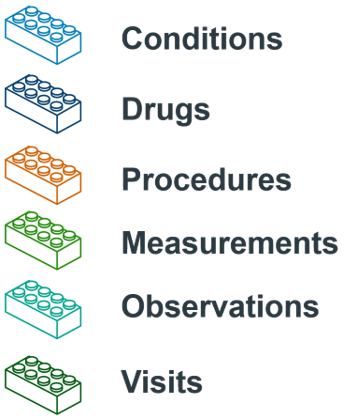
\includegraphics[width=0.5\linewidth]{images/Cohorts/cohort-legos} 

}

\caption{Building Blocks of Cohort definitions.}\label{fig:cohortLegos}
\end{figure}

When creating a cohort definition, you need to ask yourself the
following questions:

\begin{itemize}
\tightlist
\item
  \emph{What initial event defines the time of cohort entry?}
\item
  \emph{What inclusion criteria are applied to the initial events?}
\item
  \emph{What defines the time of cohort exit?}
\end{itemize}

\textbf{Cohort entry event}: The cohort entry event (initial event)
defines the time when people enter the cohort, called the \textbf{cohort
index date}. A cohort entry event can be any event recorded in the CDM
such as drug exposures, conditions, procedures, measurements and visits.
Initial events are defined by the CDM domain where the data are stored
(e.g.~PROCEDURE\_OCCURRENCE, DRUG\_EXPOSURE, etc), the concept sets
built to identify the clinical activity (e.g.~SNOMED codes for
conditions, RxNorm codes for drugs) as well as any other specific
attributes (e.g.~age at occurrence, first diagnosis/procedure/etc,
specifying start and end date, specifying visit type or criteria, days
supply, etc). The set of people having an entry event is referred to as
the \textbf{initial event cohort}. \index{cohort!entry event}

\textbf{Inclusion criteria}: Inclusion criteria are applied to the
initial event cohort to further restrict the set of people. Each
inclusion criterion is defined by the CDM domain(s) where the data are
stored, concept set(s) representing the clinical activity,
domain-specific attributes (e.g.~days supply, visit type, etc), and the
temporal logic relative to the cohort index date. Each inclusion
criterion can be evaluated to determine the impact of the criteria on
the attrition of persons from the initial event cohort. The
\textbf{qualifying cohort} is defined as all people in the initial event
cohort that satisfy all inclusion criteria.
\index{cohort!inclusion criteria}

\textbf{Cohort exit criteria}: The cohort exit event signifies when a
person no longer qualifies for cohort membership. Cohort exit can be
defined in multiple ways such as the end of the observation period, a
fixed time interval relative to the initial entry event, the last event
in a sequence of related observations (e.g.~persistent drug exposure) or
through other censoring of observation period. Cohort exit strategy will
impact whether a person can belong to the cohort multiple times during
different time intervals.\index{cohort!exit criteria}

\BeginKnitrBlock{rmdimportant}
In the OHDSI tools there is no distinction between inclusion and
exclusion criteria. All criteria are formulated as inclusion criteria.
For example, the exclusion criterium ``Exclude people with prior
hypertension'' can be formulated as the inclusion criterium ``Include
people with 0 occurrences of prior hypertension''.
\EndKnitrBlock{rmdimportant}

\section{Concept Sets}\label{conceptSets}

\index{concept set}

A concept set is an expression representing a list of concepts that can
be used as a reusable component in various analyses. It can be thought
of as a standardized, computer-executable equivalent of the code lists
often used in observational studies. A concept set expression consists
of a list of concepts with the following attributes:

\begin{itemize}
\tightlist
\item
  \textbf{Exclude}: Exclude this concept (and any of its descendants if
  selected) from the concept set.
\item
  \textbf{Descendants}: Consider not only this concept, but also all of
  its descendants.
\item
  \textbf{Mapped}: Allow to search for non-standard concepts.
\end{itemize}

For example, a concept set expression could contains two concepts as
depicted in Table \ref{tab:conceptSetExpression}. Here we include
concept
\href{http://athena.ohdsi.org/search-terms/terms/4329847}{4329847}
(``Myocardial infarction'') and all of its descendants, but exclude
concept \href{http://athena.ohdsi.org/search-terms/terms/314666}{314666}
(``Old myocardial infarction'') and all of its descendants.

\begin{longtable}[]{@{}lllll@{}}
\caption{\label{tab:conceptSetExpression} An example concept set
expression.}\tabularnewline
\toprule
Concept Id & Concept Name & Excluded & Descendants &
Mapped\tabularnewline
\midrule
\endfirsthead
\toprule
Concept Id & Concept Name & Excluded & Descendants &
Mapped\tabularnewline
\midrule
\endhead
4329847 & Myocardial infarction & NO & YES & NO\tabularnewline
314666 & Old myocardial infarction & YES & YES & NO\tabularnewline
\bottomrule
\end{longtable}

As shown in Figure \ref{fig:conceptSet}, this will include ``Myocardial
infarction'' and all of its descendants except ``Old myocardial
infarction'' and its descendants. In total, this concept set expression
implies nearly a hundred Standard Concepts. These Standard Concepts in
turn reflect hundreds of source codes (e.g.~ICD-9 and ICD-10 codes) that
may appear in the various databases.

\begin{figure}

{\centering 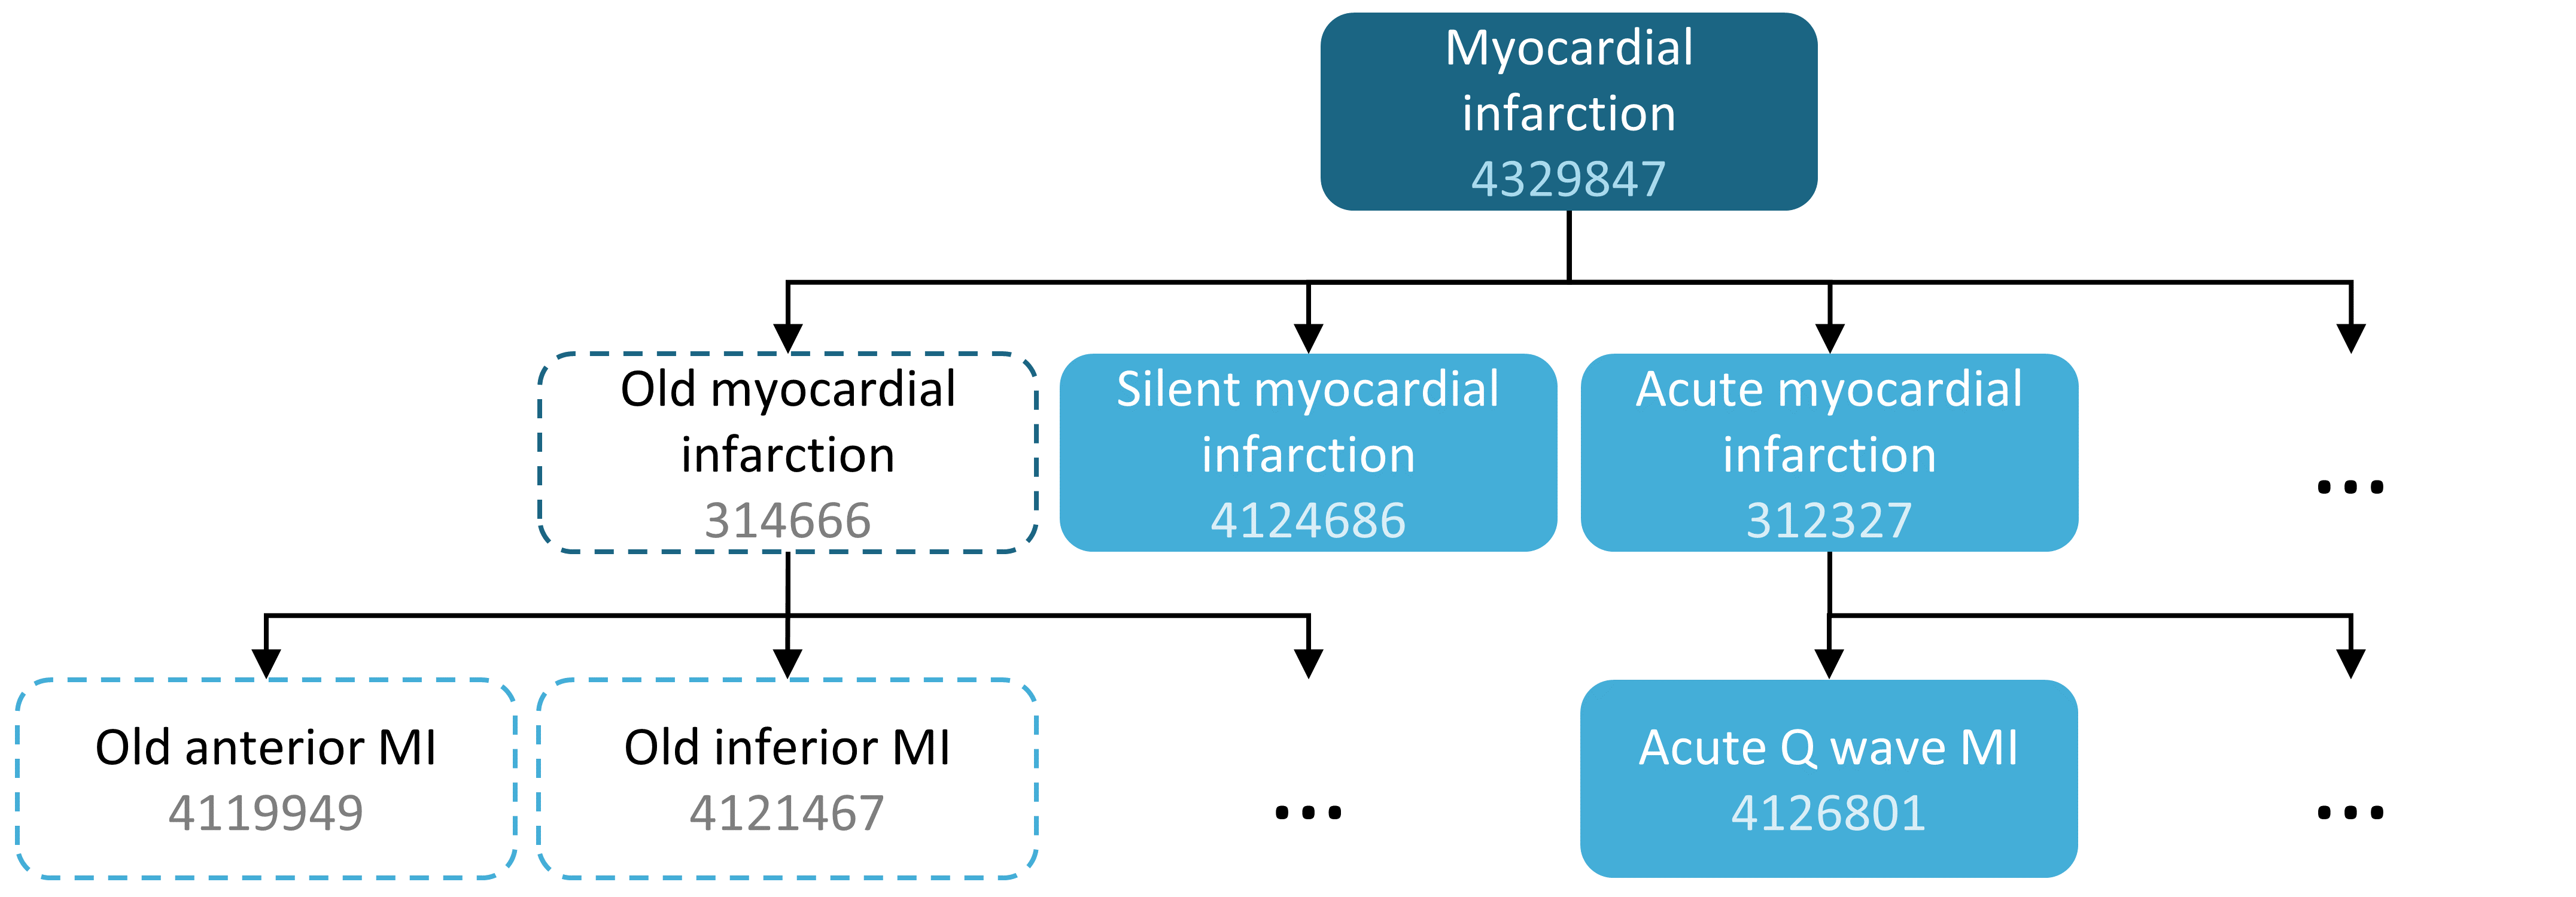
\includegraphics[width=1\linewidth]{images/Cohorts/conceptSet} 

}

\caption{A concept set including "Myocardial infaction" (with descendants), but excluding "Old myocardial infarction" (with descendants).}\label{fig:conceptSet}
\end{figure}

\section{Probabilistic Cohort
Definitions}\label{probabilistic-cohort-definitions}

Rule-based cohort definitions are a popular method for assembling cohort
definitions. However, assembling necessary expert consensus to create a
study cohort can be prohibitively time consuming. Probabilistic cohort
design is an alternative, machine-driven method to expedite the
selection of cohort attributes. In this approach, supervised machine
learning allows a phenotyping algorithm to learn from a set of labeled
examples (cases) of what attributes contribute to cohort membership.
This algorithm can then be used to better ascertain the defining
characteristics of a phenotype and what trade-offs occur in overall
study accuracy when choosing to modify phenotype criteria.
\index{cohort!probabilistic design}

An example of applying this approach on data in the CDM is the APHRODITE
(Automated PHenotype Routine for Observational Definition,
Identification, Training and Evaluation) R-package\footnote{\url{https://github.com/OHDSI/Aphrodite}}
. This package provides a cohort building framework that combines the
ability of learning from imperfectly labeled data.
\citep{Banda2017APHRODITE} \index{APHRODITE}

\section{Cohort Definition Validity}\label{cohort-definition-validity}

When you are building a cohort, you should consider which of these is
more important to you: \emph{finding all the eligible patients?} versus
\emph{Getting only the ones you are confident about?}

Your strategy to construct your cohort will depend on the clinical
stringency of how your expert consensus defines the disease. This is to
say, the right cohort design will depend on the question you're trying
to answer. You may opt to build a cohort definition that uses everything
you can get, uses the lowest common denominator so you can share it
across OHDSI sites or is a compromise of the two. It is ultimately at
the researcher's discretion what threshold of stringency is necessary to
adequately study the cohort of interest.

As mentioned at the beginning of the chapter, a cohort definition is an
attempt to infer something we would like to observe from the data that
is recorded. This begs the question how well we succeeded in that
attempt. In general, the validation of a rule-based cohort definition or
probabilistic algorithm can be thought of as a test of the proposed
cohort compared to some form of ``gold standard'' reference (e.g.~manual
chart review of cases). This is discussed in detail in Chapter
\ref{ClinicalValidity} (``Clinical Validity'').

\subsection{OHDSI Gold Standard Phenotype
Library}\label{ohdsi-gold-standard-phenotype-library}

To assist the community in the inventory and overall evaluation of
existing cohort definitions and algorithms, the OHDSI Gold Standard
Phenotype Library (GSPL) Workgroup was formed. The purpose of the GSPL
workgroup is to develop a community-backed phenotype library from
rules-based and probabilistic methods. The GSPL enable members of the
OHDSI community to find, evaluate, and utilize community-validated
cohort definitions for research and other activities. These ``gold
standard'' definitions will reside in a library, the entries of which
are held to specific standards of design and evaluation. For additional
information related to the GSPL, consult the OHDSI workgroup
page.\footnote{\url{https://www.ohdsi.org/web/wiki/doku.php?id=projects:workgroups:gold-library-wg}}
Research within this workgroup includes APHRODITE
\citep{Banda2017APHRODITE} and the PheValuator tool
\citep{Swerdel2019phevaluator} , discussed in the prior section, as well
as work done to share the Electronic Medical Records and Genomics
\href{https://emerge.mc.vanderbilt.edu/}{eMERGE}
\href{https://phekb.org/phenotypes}{Phenotype Library} across the OHDSI
network \citep{Hripcsak2019eMERGE}. If phenotype curation is your
interest, consider contributing to this workgroup.
\index{phenotype library}

\section{Defining a Cohort for
Hypertension}\label{defining-a-cohort-for-hypertension}

We begin to practice our cohort skills by putting together a cohort
definition using a rule-based approach. In this example, we want to find
\emph{patients who initiate ACE inhibitors monotherapy as first-line
treatments for hypertension}

With this context in mind, we are now going to build our cohort. As we
go through this exercise, we will approach building our cohort similar
to standard attrition chart. Figure \ref{fig:CohortPractice} shows the
logical framework for how we want to build this cohort.

\begin{figure}

{\centering 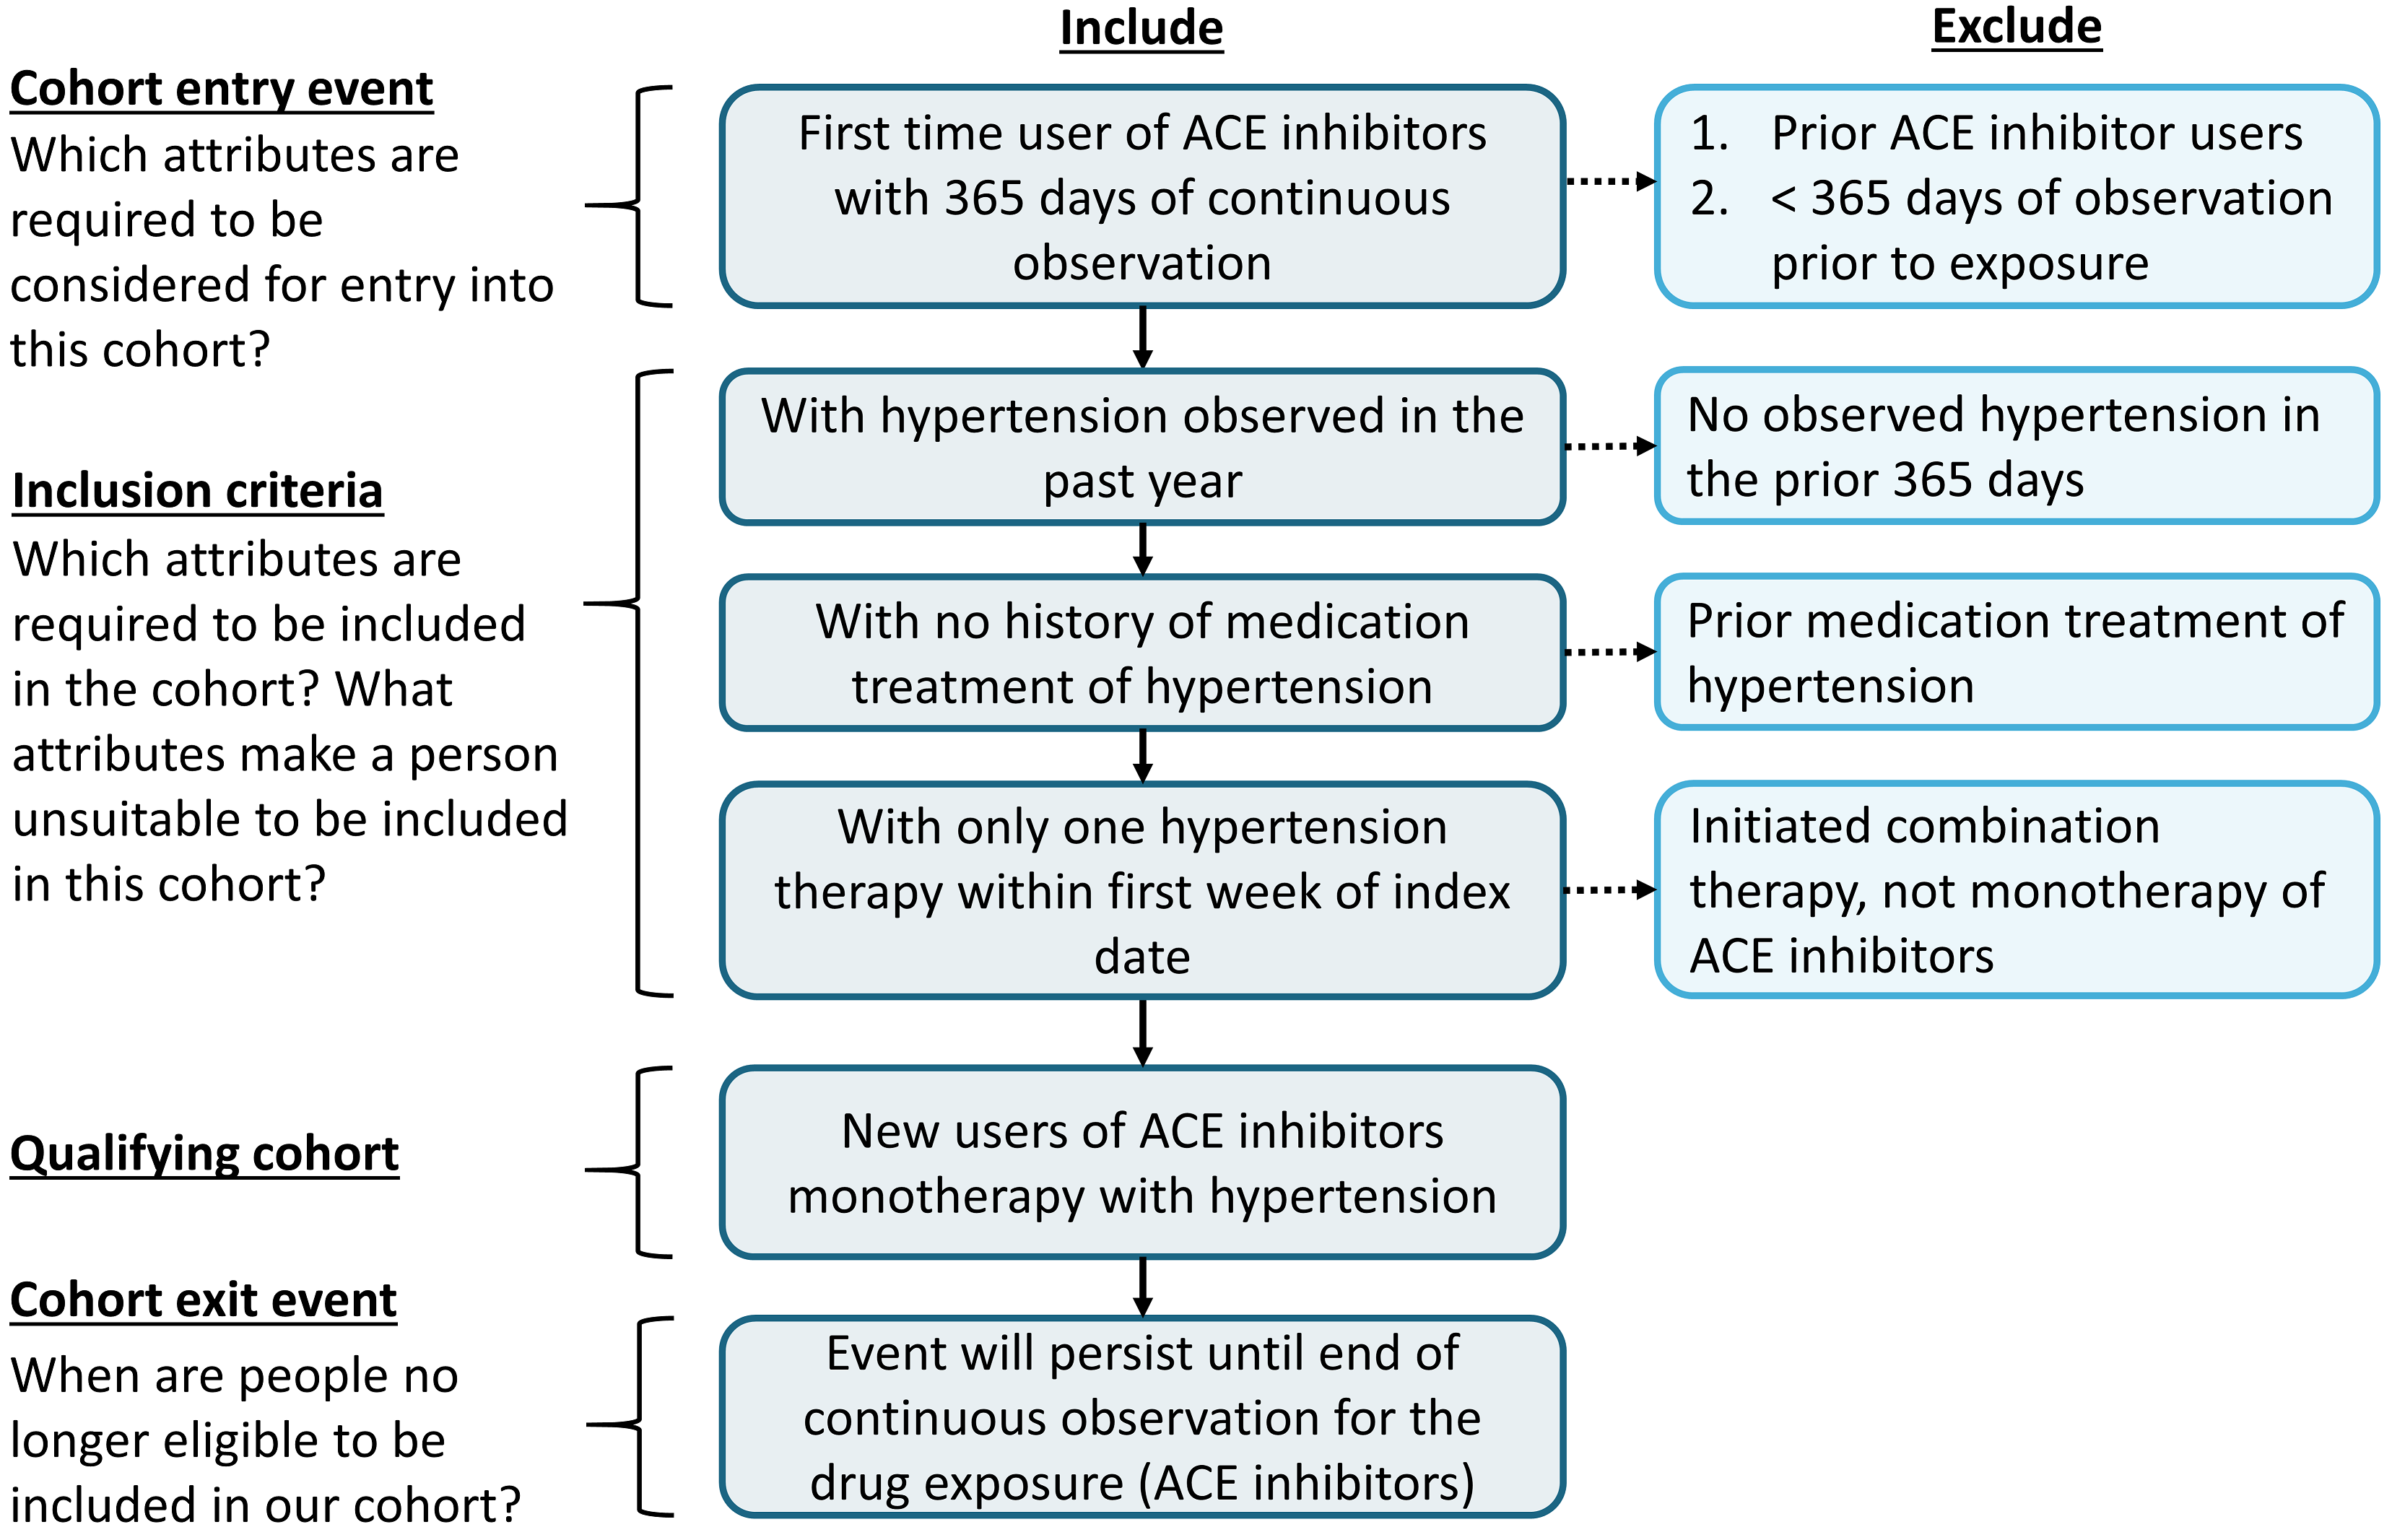
\includegraphics[width=1\linewidth]{images/Cohorts/CohortPractice} 

}

\caption{Logical Diagram of Intended Cohort}\label{fig:CohortPractice}
\end{figure}

You can build a cohort in the user interface of ATLAS or you can write a
query directly against your CDM. We will briefly discuss both in this
chapter.

\section{Implementing a Cohort Using
ATLAS}\label{implementing-a-cohort-using-atlas}

To begin in ATLAS, click on the

\includegraphics{images/Cohorts/cohortdefinition.png} module. When the
module loads, click on ``New cohort''. The next screen you will see will
be an empty cohort definition. Figure \ref{fig:ATLASdefineacohort} shows
what you will see on your screen.

\begin{figure}

{\centering 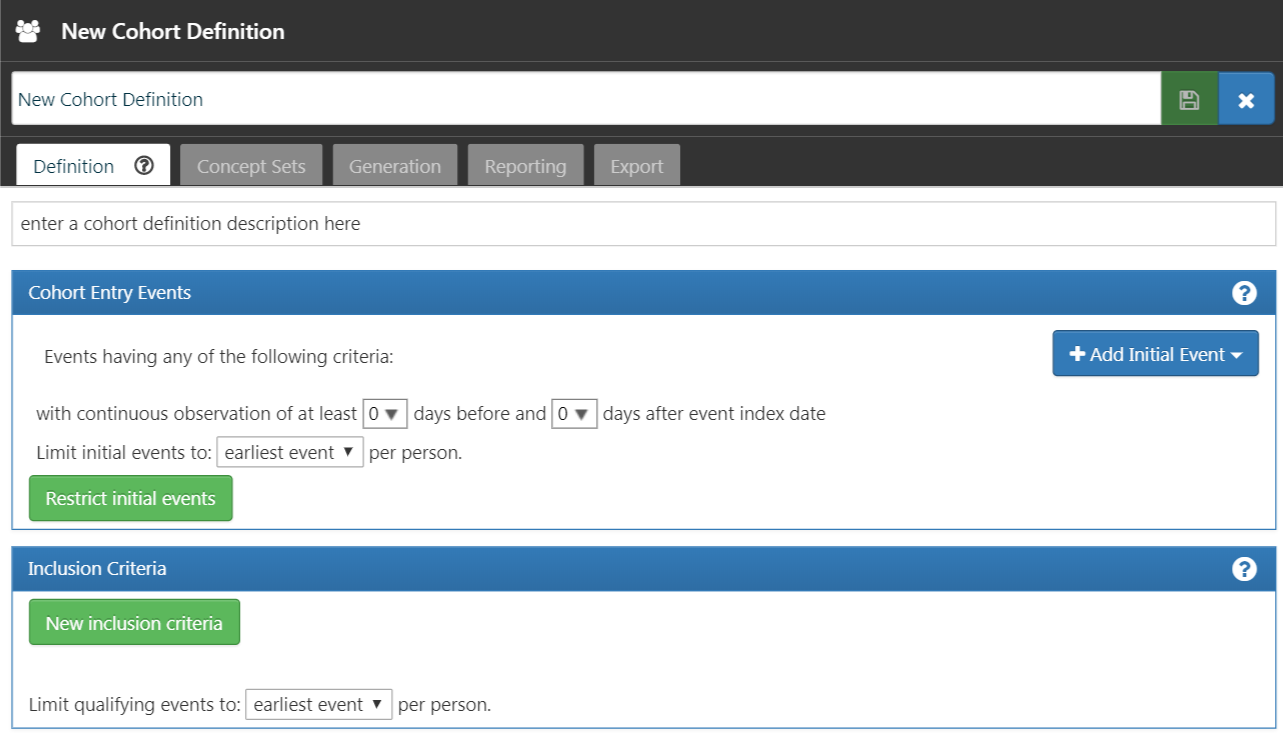
\includegraphics[width=1\linewidth]{images/Cohorts/ATLAS-defineacohort} 

}

\caption{New Cohort Definition}\label{fig:ATLASdefineacohort}
\end{figure}

Before you do anything else, you are encouraged to change the name of
the cohort from ``New Cohort Definition'' to your own unique name for
this cohort. You may opt for a name like ``New users of ACE inhibitors
as first-line monotherapy for hypertension''.

\BeginKnitrBlock{rmdimportant}
ATLAS will not allow two cohorts to have the same exact names. ATLAS
will give you a pop-up error message if you choose a name already used
by another ATLAS cohort.
\EndKnitrBlock{rmdimportant}

Once you have chosen a name, you can save the cohort by clicking

\includegraphics{images/Cohorts/save.png}.

\subsection{Initial Event Criteria}\label{initial-event-criteria}

Now we can proceed with defining the initial cohort event. You will
click ``Add initial event''. You now have to pick which domain you are
building a criteria around. You may ask yourself, ``how do I know which
domain is the initial cohort event?'' Let's figure that out.

\begin{figure}

{\centering 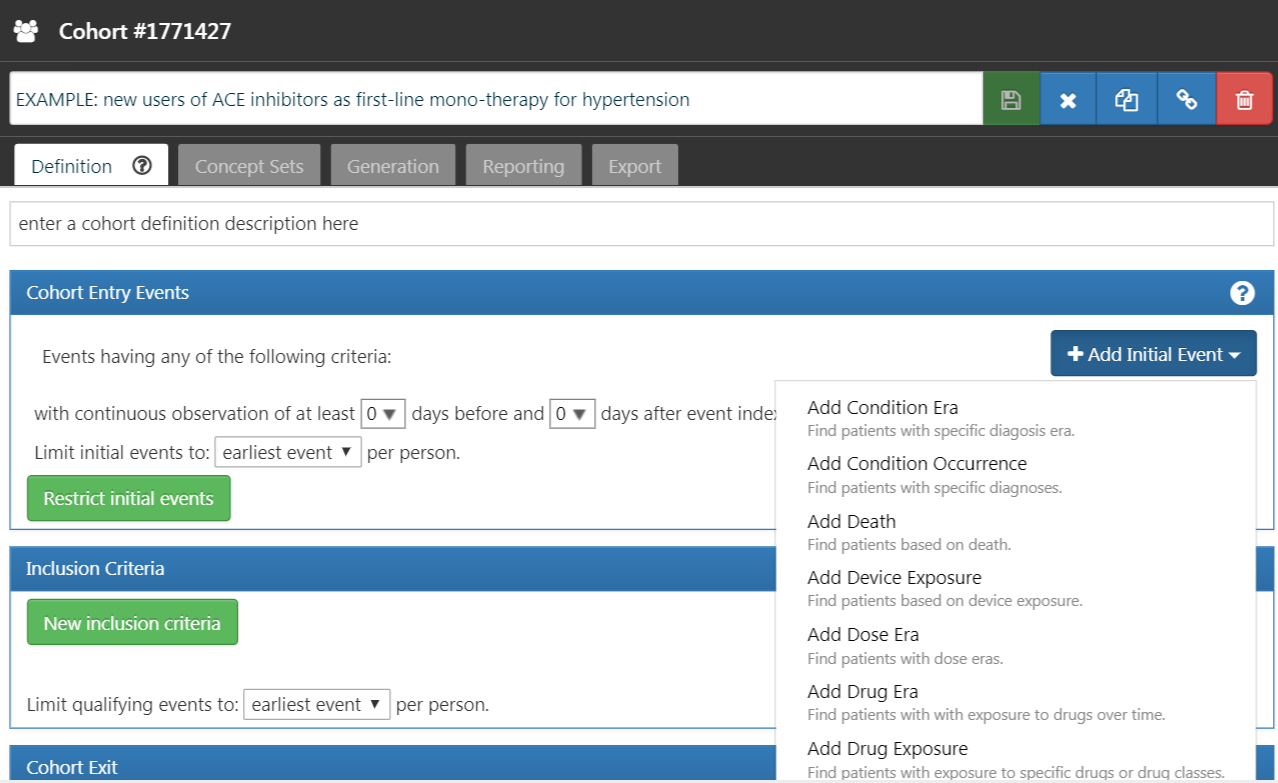
\includegraphics[width=1\linewidth]{images/Cohorts/ATLAS-initialevent} 

}

\caption{Adding an Initial Event}\label{fig:ATLASinitialevent}
\end{figure}

As we see in Figure \ref{fig:ATLASinitialevent}, ATLAS provides
descriptions below each criteria to help you. If we were building a
CONDITION\_OCCURRENCE based criteria, our question would be looking for
patients with a specific diagnosis. If we were building a DRUG\_EXPOSURE
based criteria, our question would be looking for patients with a
specific drug or drug class. Since we want to find patients who initiate
ACE inhibitors monotherapy as first-line treatments for hypertension, we
want to choose a DRUG\_EXPOSURE criteria. You may say, ``but we also
care about hypertension as a diagnosis''. You are correct. Hypertension
is another criterion we will build. However, the cohort start date is
defined by the initiation of the ACE inhibitor treatment, which is
therefore the initial event. The diagnosis of hypertension is what we
call an \emph{additional qualifying criteria}. We will return to this
once we build this criteria. We will click ``Add Drug Exposure''.

The screen will update with your selected criteria but you are not done
yet. As we see in Figure \ref{fig:ATLASdrugexposure}, ATLAS does not
know what drug we are looking for. We need to tell ATLAS which concept
set is associated to ACE inhibitors.

\begin{figure}

{\centering 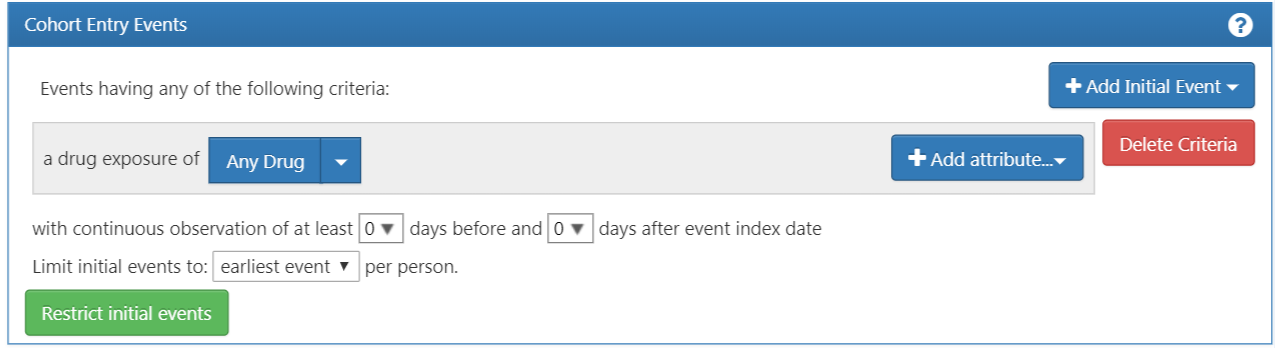
\includegraphics[width=1\linewidth]{images/Cohorts/ATLAS-drugexposure} 

}

\caption{Defining a Drug Exposure}\label{fig:ATLASdrugexposure}
\end{figure}

\subsection{Defining the Concept Set}\label{defining-the-concept-set}

You will need to click \includegraphics{images/Cohorts/downarrow.png} to
open the dialogue box that will allow you to retrieve a concept set to
define ACE Inhibitors.

\subsubsection*{Scenario 1: You Have Not Built a Concept
Set}\label{scenario-1-you-have-not-built-a-concept-set}
\addcontentsline{toc}{subsubsection}{Scenario 1: You Have Not Built a
Concept Set}

If you have not assembled your concept sets to apply to your criteria,
you will need to do so before you move forward. You may build a concept
set within the cohort definition by navigating to the ``Concept set''
tab and clicking ``New Concept Set''. You will need to rename the
concept set from ``Unnamed Concept Set'' to a name of your choosing.
From there you can use the \includegraphics{images/Cohorts/search-2.png}
module to look for clinical concepts that represent ACE inhibitors
(Figure \ref{fig:aceinhibitors}).

\begin{figure}

{\centering \includegraphics[width=1\linewidth]{images/Cohorts/aceinhibitors} 

}

\caption{Searching the Vocabulary - ACE Inhibitors}\label{fig:aceinhibitors}
\end{figure}

When you have found terms that you would like to use to define this drug
exposure, you can select the concept by clicking on
\includegraphics{images/Cohorts/shoppingcart.png}. You can return to
your cohort definition by using the left arrow in the top left of Figure
\ref{fig:aceinhibitors}. You can refer back to Chapter
\ref{StandardizedVocabularies} (Standardized Vocabularies) on how to
navigate the vocabularies to find clinical concepts of interest.

Figure \ref{fig:aceConceptSetExpression} shows our concept set
expression. We selected all ACE inhibitor ingredients we are interested
in, and include all their descendants, thus including all drugs that
contain any of these ingredients. We can click on ``Included concepts''
to see all 21,536 concepts implied by this expression, or we can click
on ``Included Source Codes'' to explore all source codes in the various
coding systems that are implied.

\begin{figure}

{\centering \includegraphics[width=1\linewidth]{images/Cohorts/aceConceptSetExpression} 

}

\caption{A concept set containing ACE inhibitor drugs.}\label{fig:aceConceptSetExpression}
\end{figure}

\subsubsection*{Scenario 2: You Have Already Built a Concept
Set}\label{scenario-2-you-have-already-built-a-concept-set}
\addcontentsline{toc}{subsubsection}{Scenario 2: You Have Already Built
a Concept Set}

If you have already created a concept set and saved it in ATLAS, you can
click to ``Import Concept Set''. A dialogue box will open that will be
prompt you to find your concept in the concept set repository of your
ATLAS as shown in Figure \ref{fig:ATLASfindyourconcept}. In the example
figure the user is retrieving concept sets stored in ATLAS. The user
typed in the name given to this concept set ``ace inhibitors'' in the
right hand search. This shortened the concept set list to only concepts
with matching names. From there, the user can click on the row of the
concept set to select it. (Note: the dialogue box will disappear once
you have selected a concept set.) You will know this action is
successful when the Any Drug box is updated with the name of the concept
set you selected.

\begin{figure}

{\centering \includegraphics[width=1\linewidth]{images/Cohorts/ATLAS-findingyourconcept} 

}

\caption{Importing a Concept Set from ATLAS Repository}\label{fig:ATLASfindyourconcept}
\end{figure}

\subsection{Additional Initial Event
Criteria}\label{additional-initial-event-criteria}

Now that you've attached a concept set, you are not done yet. Your
question is looking for new users or the first time in someone's history
they are exposed to ACE inhibitors. This translates to the \emph{first
exposure} of ACE inhibitors in the patient's record. To specify this,
you need to click ``+Add attribute''. You will want to select the ``Add
first exposure criteria''. Notice, you could specify other attributes of
a criteria you build. You could specify an attribute of age at
occurrence, the date of occurrence, gender or other attributes related
to the drug. Criteria available for selection will look different for
each domain.

From there, the window will automatically close. Once selected, this
additional attribute will show up in the same box as the initial
criteria (see Figure \ref{fig:initialEventAce}).

\BeginKnitrBlock{rmdimportant}
The current design of ATLAS may confuse some. Despite its appearance,
the \includegraphics{images/Cohorts/redX.png} is not intended to mean
``No''. It is an actionable feature to allow the user to delete the
criteria. If you click \includegraphics{images/Cohorts/redX.png}, this
criteria will go away. Thus, you need to leave the criteria with the
\includegraphics{images/Cohorts/redX.png} to keep the criteria active.
\EndKnitrBlock{rmdimportant}

Now you have built an initial qualifying event. To ensure you are
capturing the first observed drug exposure, you will want to add a
look-back window to know that you are looking at enough of the patient's
history to know what comes first. It is possible that a patient with a
short observation period may have received an exposure elsewhere that we
do not see. We cannot control this but we can mandate a minimum amount
of time the patient must be in the data prior to the index date You can
do this by adjusting the continuous observation drop downs. You could
also click the box and type in a value to these windows. We will require
365 days of continuous observation prior to the initial event. You will
update your observation period to: \emph{with continuous observation of
365 days before}, as shown in Figure \ref{fig:initialEventAce}. This
look-back window is the discretion of your study team. You may choose
differently in other cohorts. This creates, as best as we are able, a
minimum period of time we see the patient to ensure we are capturing the
first record. This criteria is about prior history and does not involve
time after the index event. Therefore, we require 0 days after the index
event. Our qualifying event is the first-ever use of ACE inhibitors.
Thus, we limit initial events to the ``earliest event'' per person.

\begin{figure}

{\centering \includegraphics[width=1\linewidth]{images/Cohorts/initialEventAce} 

}

\caption{Setting the required continuous observation before the index date.}\label{fig:initialEventAce}
\end{figure}

To further explain how this logic comes together, you can think about
assembling patient timelines.

\begin{figure}

{\centering \includegraphics[width=1\linewidth]{images/Cohorts/EarliestEventExplained} 

}

\caption{Explaining patient eligibility by criteria applied}\label{fig:EarliestEventExplained}
\end{figure}

In Figure \ref{fig:EarliestEventExplained}, each line represents a
single patient that may be eligible to join the cohort. The filled in
stars represent a time the patient fulfills the specified criteria. As
additional criteria is applied, you may see some stars are a lighter
shade. This means that these patients have other records that satisfy
the criteria but there is another record that proceeds that. By the time
we get to the last criteria, we are looking at the cumulative view of
patients who have ACE inhibitors for the first time and have 365 days
prior to the first-time occurrence. Logically, limiting to the initial
event is redundant though it is helpful to maintain our explicit logic
in every selection we make. When you are building your own cohorts, you
may opt to engage the Researchers section of the
\href{http://forums.ohdsi.org}{OHDSI Forum} to get a second opinion on
how to construct your cohort logic.

\subsection{Inclusion Criteria}\label{inclusion-criteria}

Once we have specified a cohort entry event, you could proceed to one of
two places to add your additional qualifying events: ``Restrict initial
events'' and ``New inclusion criteria''. The fundamental difference
between these two options is what interim information you want ATLAS to
serve back to you. If you add additional qualifying criteria into the
Cohort Entry Event box by selecting ``Restrict initial events'', when
you choose to generate a count in ATLAS, you will only get back the
number of people who meet ALL of these criteria. If you opt to add
criteria into the ``New inclusion criteria'', you will get an attrition
chart to show you how many patients are lost by applying additional
inclusion criteria. It is highly encouraged to utilize the Inclusion
Criteria section so you can understand the impact of each rule on the
overall success of the cohort definition. You may find a certain
inclusion criteria severely limits the number of people who end up in
the cohort. You may choose to relax this criterion to get a larger
cohort. This will ultimately be at the discretion of the expert
consensus assembling this cohort.

You will now want to click ``New inclusion criteria'' to add a
subsequent piece of logic about membership to this cohort. The
functionality in this section is identical to the way we discussed
building cohort criteria above. You may specific the criteria and add
specific attributes. Our first additional criteria is to subset the
cohort to only patients: \emph{With at least 1 occurrence of
hypertension disorder between 365 and 0 days after index date (first
initiation of an ACE inhibitor)}. You will click ``New inclusion
criteria'' to add a new criteria. You should name your criteria and, if
desired, put a little description of what you are looking for. This is
for your own purposes to recall what you build -- it will not impact the
integrity of the cohort you are defining.

Once you have annotated this new criteria, you will click on the ``+Add
criteria to group'' button to build your actual criteria for this rule.
This button functions similar to the ``Add Initial Event'' except we are
no longer specifying an initial event. We could add multiple criteria to
this -- which is why it specifies ``add criteria to group''. An example
would be if you have multiple ways of finding a disease (e.g.~logic for
a CONDITION\_OCCURRENCE, logic using a DRUG\_EXPOSURE as a proxy for
this condition, logic for using a MEASUREMENT as a proxy for this
condition). These would be separate domains and require different
criteria but can be grouped into one criteria looking for this
condition. In this case, we want to find a diagnosis of hypertension so
we ``Add condition occurrence''. We will follow similar steps as we did
with the initial event by attaching a concept set to this record. We
also want to specify the event starts between 365 days before and 0 days
after the index date (the occurrence of the first ACE inhibitor use).
Now check your logic against Figure \ref{fig:ATLASIC1}.

\begin{figure}

{\centering \includegraphics[width=1\linewidth]{images/Cohorts/ATLAS-IC1} 

}

\caption{Additional Inclusion criteria 1}\label{fig:ATLASIC1}
\end{figure}

You will then want to add another criterion to look for patients:
\emph{with exactly 0 occurrences of hypertension drugs ALL days before
and 1 day before index start date (no exposure to HT drugs before an ACE
inhibitor)}. This process begins as we did before by clicking the ``New
inclusion criteria'' button, adding your annotations to this criterion
and then clicking ``+Add criteria to group''. This is a DRUG\_EXPOSURE
so you will click ``Add Drug Exposure'', attach a concept set for
hypertensive drugs, and will specify ALL days before and 0 days after
the index date. Make sure to confirm you have \emph{exactly 0}
occurrence selected. Now check your logic against Figure
\ref{fig:ATLASIC2}.

\begin{figure}

{\centering \includegraphics[width=1\linewidth]{images/Cohorts/ATLAS-IC2} 

}

\caption{Additional Inclusion Criteria 2}\label{fig:ATLASIC2}
\end{figure}

You may be confused why ``having no occurrences'' is coded as ``exactly
0 occurrences.'' This is a nuance of how ATLAS consumes knowledge. ATLAS
only consumes inclusion criteria. You must use logical operators to
indicate when you want the absence of a specific attribute such as:
``Exactly 0.'' Over time you will become more familiar with the logical
operators available in ATLAS criteria.

Lastly, you will want to add your another criterion to look for
patients: \emph{with exactly 1 occurrence of hypertension drugs between
0 days before and 7 days after index start date AND can only start one
HT drug (an ACE inhibitor)} . This process begins as we did before by
clicking the ``New inclusion criteria'' button, adding your annotations
to this criterion and then clicking ``+Add criteria to group''. This is
a DRUG\_EXPOSURE so you will click ``Add Drug Exposure'', attach a
concept set for hypertensive drugs, and will specify 0 days before and 7
days after the index date. Now check your logic against Figure
\ref{fig:ATLASIC3}.

\begin{figure}

{\centering \includegraphics[width=1\linewidth]{images/Cohorts/ATLAS-IC3} 

}

\caption{Additional Inclusion Criteria 3}\label{fig:ATLASIC3}
\end{figure}

\subsection{Cohort Exit Criteria}\label{cohort-exit-criteria}

You have now added all of your qualifying inclusion criteria. You must
now specify your cohort exit criteria. You will ask yourself, ``when are
people no longer eligible to be included in this cohort?'' In this
cohort, we are following new-users of a drug exposure. We want to look
at continuous observation period as it relates to the drug exposure. As
such, the exit criterion is specified to follow for the entirety of the
continuous drug exposure. If there is a subsequent break in the drug
exposure, the patient will exit the cohort at this time. We do this as
we cannot determine what happened to the person during the break in the
drug exposure. We can also set a criteria on the persistence window to
specify an allowable gap between drug exposures. In this case, our
experts leading this study concluded that a maximum of 30 days between
exposure records is allowable when inferring the era of persistence
exposure.

\textbf{Why are gaps allowed?} In some data sets, we see only portions
of clinical interactions. Drug exposures, in particular, may represent a
dispense of a prescription that can cover a certain period of time.
Thus, we allow a certain amount of time between drug exposures as we
know the patient may logically still have access to the initial drug
exposure because the unit of dispense exceeded one day.

We can configure this by selecting the Event will persist ``end of a
continuous drug exposure''. We then will add our persistence window to
``allow for a maximum of 30 days'' and append the concept set for ``ACE
inhibitors''. Now check your logic against Figure
\ref{fig:ATLAScohortexit}.

\begin{figure}

{\centering \includegraphics[width=1\linewidth]{images/Cohorts/cohort-exit} 

}

\caption{Cohort Exit Criteria}\label{fig:ATLAScohortexit}
\end{figure}

In the case of this cohort, there are no other censoring events.
However, you may build other cohorts where you need to specify this
criteria. You would proceed similarly to the way we have added other
attributes to this cohort definition. You have now successfully finished
creating your cohort. Make sure to hit the
\includegraphics{images/Cohorts/save.png} button. Congratulations!
Building a cohort is the most important building block of answering a
question in the OHDSI tools. You can now use the ``Export'' tab to share
your cohort definition to other collaborators in the form of SQL code or
JSON files to load into ATLAS.

\section{Implementing the Cohort Using
SQL}\label{implementing-the-cohort-using-sql}

Here we describe how to create the same cohort, but using SQL and R. As
discussed in Chapter \ref{SqlAndR}, OHDSI provides two R packages,
called SqlRender and DatabaseConnector, which together allow writing SQL
code that can be automatically translated and executed against a wide
variety of database platforms.

For clarity, we will split the SQL into several chunks, each chunk
generating a temp table that is used in the next. This is likely not the
most computationally efficient way to do it, but it is easier to read
than a single very long statement.

\subsection{Connecting to the
Database}\label{connecting-to-the-database}

We first need to tell R how to connect to the server. We use the
\href{https://ohdsi.github.io/DatabaseConnector/}{DatabaseConnector}
package, which provides a function called
\texttt{createConnectionDetails}. Type \texttt{?createConnectionDetails}
for the specific settings required for the various database management
systems (DBMS). For example, one might connect to a PostgreSQL database
using this code:

\begin{Shaded}
\begin{Highlighting}[]
\KeywordTok{library}\NormalTok{(CohortMethod)}
\NormalTok{connDetails <-}\StringTok{ }\KeywordTok{createConnectionDetails}\NormalTok{(}\DataTypeTok{dbms =} \StringTok{"postgresql"}\NormalTok{,}
                                       \DataTypeTok{server =} \StringTok{"localhost/ohdsi"}\NormalTok{,}
                                       \DataTypeTok{user =} \StringTok{"joe"}\NormalTok{,}
                                       \DataTypeTok{password =} \StringTok{"supersecret"}\NormalTok{)}

\NormalTok{cdmDbSchema <-}\StringTok{ "my_cdm_data"}
\NormalTok{cohortDbSchema <-}\StringTok{ "scratch"}
\NormalTok{cohortTable <-}\StringTok{ "my_cohorts"}
\end{Highlighting}
\end{Shaded}

The last three lines define the \texttt{cdmDbSchema},
\texttt{cohortDbSchema}, and \texttt{cohortTable} variables. We will use
these later to tell R where the data in CDM format live, and where the
cohorts of interest have to be created. Note that for Microsoft SQL
Server, database schemas need to specify both the database and the
schema, so for example
\texttt{cdmDbSchema\ \textless{}-\ "my\_cdm\_data.dbo"}.

\subsection{Specifying the Concepts}\label{specifying-the-concepts}

For readability we will define the concept IDs we need in R, and pass
them to the SQL:

\begin{Shaded}
\begin{Highlighting}[]
\NormalTok{aceI <-}\StringTok{ }\KeywordTok{c}\NormalTok{(}\DecValTok{1308216}\NormalTok{, }\DecValTok{1310756}\NormalTok{, }\DecValTok{1331235}\NormalTok{, }\DecValTok{1334456}\NormalTok{, }\DecValTok{1335471}\NormalTok{, }\DecValTok{1340128}\NormalTok{, }\DecValTok{1341927}\NormalTok{,}
          \DecValTok{1342439}\NormalTok{, }\DecValTok{1363749}\NormalTok{, }\DecValTok{1373225}\NormalTok{)}

\NormalTok{hypertension <-}\StringTok{ }\DecValTok{316866}

\NormalTok{allHtDrugs <-}\StringTok{ }\KeywordTok{c}\NormalTok{(}\DecValTok{904542}\NormalTok{, }\DecValTok{907013}\NormalTok{, }\DecValTok{932745}\NormalTok{, }\DecValTok{942350}\NormalTok{, }\DecValTok{956874}\NormalTok{, }\DecValTok{970250}\NormalTok{, }\DecValTok{974166}\NormalTok{,}
                  \DecValTok{978555}\NormalTok{, }\DecValTok{991382}\NormalTok{, }\DecValTok{1305447}\NormalTok{, }\DecValTok{1307046}\NormalTok{, }\DecValTok{1307863}\NormalTok{, }\DecValTok{1308216}\NormalTok{,}
                  \DecValTok{1308842}\NormalTok{, }\DecValTok{1309068}\NormalTok{, }\DecValTok{1309799}\NormalTok{, }\DecValTok{1310756}\NormalTok{, }\DecValTok{1313200}\NormalTok{, }\DecValTok{1314002}\NormalTok{,}
                  \DecValTok{1314577}\NormalTok{, }\DecValTok{1317640}\NormalTok{, }\DecValTok{1317967}\NormalTok{, }\DecValTok{1318137}\NormalTok{, }\DecValTok{1318853}\NormalTok{, }\DecValTok{1319880}\NormalTok{,}
                  \DecValTok{1319998}\NormalTok{, }\DecValTok{1322081}\NormalTok{, }\DecValTok{1326012}\NormalTok{, }\DecValTok{1327978}\NormalTok{, }\DecValTok{1328165}\NormalTok{, }\DecValTok{1331235}\NormalTok{,}
                  \DecValTok{1332418}\NormalTok{, }\DecValTok{1334456}\NormalTok{, }\DecValTok{1335471}\NormalTok{, }\DecValTok{1338005}\NormalTok{, }\DecValTok{1340128}\NormalTok{, }\DecValTok{1341238}\NormalTok{,}
                  \DecValTok{1341927}\NormalTok{, }\DecValTok{1342439}\NormalTok{, }\DecValTok{1344965}\NormalTok{, }\DecValTok{1345858}\NormalTok{, }\DecValTok{1346686}\NormalTok{, }\DecValTok{1346823}\NormalTok{,}
                  \DecValTok{1347384}\NormalTok{, }\DecValTok{1350489}\NormalTok{, }\DecValTok{1351557}\NormalTok{, }\DecValTok{1353766}\NormalTok{, }\DecValTok{1353776}\NormalTok{, }\DecValTok{1363053}\NormalTok{,}
                  \DecValTok{1363749}\NormalTok{, }\DecValTok{1367500}\NormalTok{, }\DecValTok{1373225}\NormalTok{, }\DecValTok{1373928}\NormalTok{, }\DecValTok{1386957}\NormalTok{, }\DecValTok{1395058}\NormalTok{,}
                  \DecValTok{1398937}\NormalTok{, }\DecValTok{40226742}\NormalTok{, }\DecValTok{40235485}\NormalTok{)}
\end{Highlighting}
\end{Shaded}

\subsection{Finding First Use}\label{finding-first-use}

We will first find first use of ACE inhibitors for each patient:

\begin{Shaded}
\begin{Highlighting}[]
\NormalTok{conn <-}\StringTok{ }\KeywordTok{connect}\NormalTok{(connectionDetails)}

\NormalTok{sql <-}\StringTok{ "SELECT person_id AS subject_id,}
\StringTok{  MIN(drug_exposure_start_date) AS cohort_start_date}
\StringTok{INTO #first_use}
\StringTok{FROM @cdm_db_schema.drug_exposure}
\StringTok{INNER JOIN @cdm_db_schema.concept_ancestor}
\StringTok{  ON descendant_concept_id = drug_concept_id}
\StringTok{WHERE ancestor_concept_id IN (@ace_i)}
\StringTok{GROUP BY person_id;"}

\KeywordTok{renderTranslateExecuteSql}\NormalTok{(conn, }
\NormalTok{                          sql, }
                          \DataTypeTok{cdm_db_schema =}\NormalTok{ cdmDbSchema, }
                          \DataTypeTok{ace_i =}\NormalTok{ aceI)}
\end{Highlighting}
\end{Shaded}

Note that we join the DRUG\_EXPOSURE table to the CONCEPT\_ANCESTOR
table to find all drugs that contain an ACE inhibitor.

\subsection{Require 365 Days of Prior
Observation}\label{require-365-days-of-prior-observation}

Next, we require 365 of continuous prior observation by joining to the
OBSERVATION\_PERIOD table:

\begin{Shaded}
\begin{Highlighting}[]
\NormalTok{sql <-}\StringTok{ "SELECT subject_id,}
\StringTok{  cohort_start_date}
\StringTok{INTO #has_prior_obs}
\StringTok{FROM #first_use}
\StringTok{INNER JOIN @cdm_db_schema.observation_period}
\StringTok{  ON subject_id = person_id}
\StringTok{    AND observation_period_start_date <= cohort_start_date}
\StringTok{    AND observation_period_end_date >= cohort_start_date}
\StringTok{WHERE DATEADD(DAY, 365, observation_period_start_date) < cohort_start_date;"}

\KeywordTok{renderTranslateExecuteSql}\NormalTok{(conn, sql, }\DataTypeTok{cdm_db_schema =}\NormalTok{ cdmDbSchema)}
\end{Highlighting}
\end{Shaded}

\subsection{Require Prior
Hypertension}\label{require-prior-hypertension}

We require a hypertension diagnosis in the 365 days prior:

\begin{Shaded}
\begin{Highlighting}[]
\NormalTok{sql <-}\StringTok{ "SELECT DISTINCT subject_id,}
\StringTok{  cohort_start_date}
\StringTok{INTO #has_ht}
\StringTok{FROM #has_prior_obs}
\StringTok{INNER JOIN @cdm_db_schema.condition_occurrence}
\StringTok{  ON subject_id = person_id}
\StringTok{    AND condition_start_date <= cohort_start_date}
\StringTok{    AND condition_start_date >= DATEADD(DAY, -365, cohort_start_date)}
\StringTok{INNER JOIN @cdm_db_schema.concept_ancestor}
\StringTok{  ON descendant_concept_id = condition_concept_id}
\StringTok{WHERE ancestor_concept_id = @hypertension;"}

\KeywordTok{renderTranslateExecuteSql}\NormalTok{(conn, }
\NormalTok{                          sql, }
                          \DataTypeTok{cdm_db_schema =}\NormalTok{ cdmDbSchema, }
                          \DataTypeTok{hypertension =}\NormalTok{ hypertension)}
\end{Highlighting}
\end{Shaded}

Note that we \texttt{SELECT\ DISTINCT}, because else if a person has
multiple hypertension diagnoses in their past, we would create duplicate
cohort entries.

\subsection{No Prior Treatment}\label{no-prior-treatment}

We require no prior exposure to any hypertension treatment:

\begin{Shaded}
\begin{Highlighting}[]
\NormalTok{sql <-}\StringTok{ "SELECT subject_id,}
\StringTok{  cohort_start_date}
\StringTok{INTO #no_prior_ht_drugs}
\StringTok{FROM #has_ht}
\StringTok{LEFT JOIN (}
\StringTok{  SELECT *}
\StringTok{  FROM @cdm_db_schema.drug_exposure}
\StringTok{  INNER JOIN @cdm_db_schema.concept_ancestor}
\StringTok{    ON descendant_concept_id = drug_concept_id}
\StringTok{  WHERE ancestor_concept_id IN (@all_ht_drugs)}
\StringTok{) ht_drugs}
\StringTok{  ON subject_id = person_id}
\StringTok{    AND drug_exposure_start_date < cohort_start_date}
\StringTok{WHERE person_id IS NULL;"}

\KeywordTok{renderTranslateExecuteSql}\NormalTok{(conn, }
\NormalTok{                          sql, }
                          \DataTypeTok{cdm_db_schema =}\NormalTok{ cdmDbSchema, }
                          \DataTypeTok{all_ht_drugs =}\NormalTok{ allHtDrugs)}
\end{Highlighting}
\end{Shaded}

Note that we use a left join, and only allow rows where the person\_id,
which comes from the DRUG\_EXPOSURE table is NULL, meaning no matching
record was found.

\subsection{Monotherapy}\label{monotherapy}

We require there to be only one exposure to hypertension treatment in
the first seven days of the cohort entry:

\begin{Shaded}
\begin{Highlighting}[]
\NormalTok{sql <-}\StringTok{ "SELECT subject_id,}
\StringTok{  cohort_start_date}
\StringTok{INTO #monotherapy}
\StringTok{FROM #no_prior_ht_drugs}
\StringTok{INNER JOIN @cdm_db_schema.drug_exposure}
\StringTok{  ON subject_id = person_id}
\StringTok{    AND drug_exposure_start_date >= cohort_start_date}
\StringTok{    AND drug_exposure_start_date <= DATEADD(DAY, 7, cohort_start_date)}
\StringTok{INNER JOIN @cdm_db_schema.concept_ancestor}
\StringTok{  ON descendant_concept_id = drug_concept_id}
\StringTok{WHERE ancestor_concept_id IN (@all_ht_drugs)}
\StringTok{GROUP BY subject_id,}
\StringTok{  cohort_start_date}
\StringTok{HAVING COUNT(*) = 1;"}

\KeywordTok{renderTranslateExecuteSql}\NormalTok{(conn, }
\NormalTok{                          sql, }
                          \DataTypeTok{cdm_db_schema =}\NormalTok{ cdmDbSchema, }
                          \DataTypeTok{all_ht_drugs =}\NormalTok{ allHtDrugs)}
\end{Highlighting}
\end{Shaded}

\subsection{Cohort Exit}\label{cohort-exit}

We have now fully specified our cohort except the cohort end date. The
cohort is defined to end when the exposure stops, allowing for a maximum
30-day gap between subsequent exposures. This means we need to not only
consider the first drug exposure, but also subsequent drug exposures to
ACE inhibitors. The SQL for combining subsequent exposures into eras can
be highly complex. Luckily, standard code has been defined that can
efficiently create eras. (This code was written by Chris Knoll, and is
often referred to within OHDSI as `the magic'). We first create a temp
table containing all exposures we wish to merge:

\begin{Shaded}
\begin{Highlighting}[]
\NormalTok{sql <-}\StringTok{ "}
\StringTok{  SELECT person_id,}
\StringTok{    CAST(1 AS INT) AS concept_id,}
\StringTok{    drug_exposure_start_date AS exposure_start_date,}
\StringTok{    drug_exposure_end_date AS exposure_end_date}
\StringTok{  INTO #exposure}
\StringTok{  FROM @cdm_db_schema.drug_exposure}
\StringTok{  INNER JOIN @cdm_db_schema.concept_ancestor}
\StringTok{    ON descendant_concept_id = drug_concept_id}
\StringTok{  WHERE ancestor_concept_id IN (@ace_i);"}
\KeywordTok{renderTranslateExecuteSql}\NormalTok{(conn,}
\NormalTok{                          sql, }
                          \DataTypeTok{cdm_db_schema =}\NormalTok{ cdmDbSchema, }
                          \DataTypeTok{ace_i =}\NormalTok{ aceI)}
\end{Highlighting}
\end{Shaded}

We then run the standard code for merging sequential exposures:

\begin{Shaded}
\begin{Highlighting}[]
\NormalTok{sql <-}\StringTok{ "}
\StringTok{SELECT ends.person_id AS subject_id,}
\StringTok{    ends.concept_id AS cohort_definition_id,}
\StringTok{  MIN(exposure_start_date) AS cohort_start_date,}
\StringTok{  ends.era_end_date AS cohort_end_date}
\StringTok{INTO #exposure_era}
\StringTok{FROM (}
\StringTok{  SELECT exposure.person_id,}
\StringTok{    exposure.concept_id,}
\StringTok{    exposure.exposure_start_date,}
\StringTok{    MIN(events.end_date) AS era_end_date}
\StringTok{  FROM #exposure exposure}
\StringTok{  JOIN (}
\StringTok{--cteEndDates}
\StringTok{    SELECT person_id,}
\StringTok{      concept_id,}
\StringTok{      DATEADD(DAY, - 1 * @max_gap, event_date) AS end_date}
\StringTok{    FROM (}
\StringTok{      SELECT person_id,}
\StringTok{        concept_id,}
\StringTok{        event_date,}
\StringTok{        event_type,}
\StringTok{        MAX(start_ordinal) OVER (}
\StringTok{          PARTITION BY person_id ,concept_id ORDER BY event_date,}
\StringTok{              event_type ROWS UNBOUNDED PRECEDING}
\StringTok{          ) AS start_ordinal,}
\StringTok{        ROW_NUMBER() OVER (}
\StringTok{          PARTITION BY person_id, concept_id ORDER BY event_date,}
\StringTok{            event_type}
\StringTok{          ) AS overall_ord}
\StringTok{      FROM (}
\StringTok{-- select the start dates, assigning a row number to each}
\StringTok{        SELECT person_id,}
\StringTok{          concept_id,}
\StringTok{          exposure_start_date AS event_date,}
\StringTok{          0 AS event_type,}
\StringTok{          ROW_NUMBER() OVER (}
\StringTok{            PARTITION BY person_id, concept_id ORDER BY exposure_start_date}
\StringTok{            ) AS start_ordinal}
\StringTok{        FROM #exposure exposure}

\StringTok{        UNION ALL}
\StringTok{-- add the end dates with NULL as the row number, padding the end dates by}
\StringTok{-- @max_gap to allow a grace period for overlapping ranges.}

\StringTok{        SELECT person_id,}
\StringTok{          concept_id,}
\StringTok{          DATEADD(day, @max_gap, exposure_end_date),}
\StringTok{          1 AS event_type,}
\StringTok{          NULL}
\StringTok{        FROM #exposure exposure}
\StringTok{        ) rawdata}
\StringTok{    ) events}
\StringTok{  WHERE 2 * events.start_ordinal - events.overall_ord = 0}
\StringTok{  ) events}
\StringTok{  ON exposure.person_id = events.person_id}
\StringTok{      AND exposure.concept_id = events.concept_id}
\StringTok{      AND events.end_date >= exposure.exposure_end_date}
\StringTok{  GROUP BY exposure.person_id,}
\StringTok{      exposure.concept_id,}
\StringTok{      exposure.exposure_start_date}
\StringTok{  ) ends}
\StringTok{GROUP BY ends.person_id,}
\StringTok{  concept_id,}
\StringTok{  ends.era_end_date;"}

\KeywordTok{renderTranslateExecuteSql}\NormalTok{(conn,}
\NormalTok{                          sql, }
                          \DataTypeTok{cdm_db_schema =}\NormalTok{ cdmDbSchema,}
                          \DataTypeTok{max_gap =} \DecValTok{30}\NormalTok{)}
\end{Highlighting}
\end{Shaded}

This code merges all subsequent exposures, allowing for a gap between
exposures as defined by the \texttt{max\_gap} argument. The resulting
drug exposure eras are written to a temp table called
\texttt{\#exposure\_era}.

Next, we simply join these ACE inhibitor exposure eras to our original
cohort to use the era end dates as our cohort end dates:

\begin{Shaded}
\begin{Highlighting}[]
\NormalTok{sql <-}\StringTok{ "SELECT ee.subject_id,}
\StringTok{  CAST(1 AS INT) AS cohort_definition_id,}
\StringTok{  ee.cohort_start_date,}
\StringTok{  ee.cohort_end_date}
\StringTok{INTO @cohort_db_schema.@cohort_table}
\StringTok{FROM #monotherapy mt}
\StringTok{INNER JOIN #exposure_era ee}
\StringTok{  ON mt.subject_id = ee.subject_id}
\StringTok{    AND mt.cohort_start_date = ee.cohort_start_date;"}

\KeywordTok{renderTranslateExecuteSql}\NormalTok{(conn, }
\NormalTok{                          sql, }
                          \DataTypeTok{cohort_db_schema =}\NormalTok{ cohortDbSchema, }
                          \DataTypeTok{cohort_table =}\NormalTok{ cohortTable)}
\end{Highlighting}
\end{Shaded}

Here we store the final cohort in schema and table we defined earlier.
We assign it a cohort definition ID of 1, to distinguish it from other
cohorts we may wish to store in the same table.

\subsection{Cleanup}\label{cleanup}

Finally, it is always recommend to clean up any temp tables that were
created, and disconnect from the database server:

\begin{Shaded}
\begin{Highlighting}[]
\NormalTok{sql <-}\StringTok{ "TRUNCATE TABLE #first_use;}
\StringTok{DROP TABLE #first_use;}

\StringTok{TRUNCATE TABLE #has_prior_obs;}
\StringTok{DROP TABLE #has_prior_obs;}

\StringTok{TRUNCATE TABLE #has_ht;}
\StringTok{DROP TABLE #has_ht;}

\StringTok{TRUNCATE TABLE #no_prior_ht_drugs;}
\StringTok{DROP TABLE #no_prior_ht_drugs;}

\StringTok{TRUNCATE TABLE #monotherapy;}
\StringTok{DROP TABLE #monotherapy;}

\StringTok{TRUNCATE TABLE #exposure;}
\StringTok{DROP TABLE #exposure;}

\StringTok{TRUNCATE TABLE #exposure_era;}
\StringTok{DROP TABLE #exposure_era;"}

\KeywordTok{renderTranslateExecuteSql}\NormalTok{(conn, sql)}

\KeywordTok{disconnect}\NormalTok{(conn)}
\end{Highlighting}
\end{Shaded}

\section{Summary}\label{summary-8}

\BeginKnitrBlock{rmdsummary}
\begin{itemize}
\item
  A cohort is set of persons who satisfy one or more inclusion criteria
  for a duration of time.
\item
  A cohort definition is the description of logic used for identifying a
  particular cohort.
\item
  Cohorts are used (and re-used) throughout the OHDSI analytics tools to
  define for example the exposures and outcomes of interest.
\item
  There are two major approaches to building a cohort: rule-based and
  probabilistic.
\item
  Rule-based cohort definitions can be created in ATLAS, or using SQL
\end{itemize}
\EndKnitrBlock{rmdsummary}

\section{Exercises}\label{exercises-5}

\subsubsection*{Prerequisites}\label{prerequisites-4}
\addcontentsline{toc}{subsubsection}{Prerequisites}

For the first exercise, access to an ATLAS instance is required. You can
use the instance at \url{http://atlas-demo.ohdsi.org}, or any other
instance you have acces to.

\BeginKnitrBlock{exercise}
\protect\hypertarget{exr:exerciseCohortsAtlas}{}{\label{exr:exerciseCohortsAtlas}
}Use ATLAS to create a cohort definition following these criteria:

\begin{itemize}
\tightlist
\item
  New users of diclofenac
\item
  Ages 16 or older
\item
  With at least 365 days of continuous observation prior to exposure
\item
  Without prior exposure to any NSAID (Non-Steroidal Anti-Inflammatory
  Drug)
\item
  Without prior diagnosis of cancer
\item
  With cohort exit defined as discontinuation of exposure (allowing for
  a 30-day gap)
\end{itemize}
\EndKnitrBlock{exercise}

\subsubsection*{Prerequisites}\label{prerequisites-5}
\addcontentsline{toc}{subsubsection}{Prerequisites}

For the second exercise we assume R, R-Studio and Java have been
installed as described in Section \ref{installR}. Also required are the
\href{https://ohdsi.github.io/SqlRender/}{SqlRender},
\href{https://ohdsi.github.io/DatabaseConnector/}{DatabaseConnector},
and \href{https://ohdsi.github.io/Eunomia/}{Eunomia} packages, which can
be installed using:

\begin{Shaded}
\begin{Highlighting}[]
\KeywordTok{install.packages}\NormalTok{(}\KeywordTok{c}\NormalTok{(}\StringTok{"SqlRender"}\NormalTok{, }\StringTok{"DatabaseConnector"}\NormalTok{, }\StringTok{"devtools"}\NormalTok{))}
\NormalTok{devtools}\OperatorTok{::}\KeywordTok{install_github}\NormalTok{(}\StringTok{"ohdsi/Eunomia"}\NormalTok{, }\DataTypeTok{ref =} \StringTok{"v1.0.0"}\NormalTok{)}
\end{Highlighting}
\end{Shaded}

The Eunomia package provides a simulated dataset in the CDM that will
run inside your local R session. The connection details can be obtained
using:

\begin{Shaded}
\begin{Highlighting}[]
\NormalTok{connectionDetails <-}\StringTok{ }\NormalTok{Eunomia}\OperatorTok{::}\KeywordTok{getEunomiaConnectionDetails}\NormalTok{()}
\end{Highlighting}
\end{Shaded}

The CDM database schema is ``main''.

\BeginKnitrBlock{exercise}
\protect\hypertarget{exr:exerciseCohortsSql}{}{\label{exr:exerciseCohortsSql}
}Use SQL and R to create a cohort for acute myocardial infarction (AMI)
in the existing COHORT table, following these criteria:

\begin{itemize}
\tightlist
\item
  An occurrence of a myocardial infarction diagnose (concept 4329847
  ``Myocardial infarction'' and all of its descendants, excluding
  concept 314666 ``Old myocardial infarction'' and any of its
  descendants).
\item
  During an inpatient or ER visit (concepts 9201, 9203, and 262 for
  ``Inpatient visit'', ``Emergency Room Visit'', and ``Emergency Room
  and Inpatient Visit'', respectively).
\end{itemize}
\EndKnitrBlock{exercise}

Suggested answers can be found in Appendix \ref{Cohortsanswers}.

\chapter{Characterization}\label{Characterization}

\emph{Chapter leads: Anthony Sena \& Daniel Prieto-Alhambra}

Observational healthcare databases provide a valuable resource to
understand variations in populations based on a host of characteristics.
Characterizing populations through the use of descriptive statistics is
an important first step in generating hypotheses about the determinants
of health and disease. In this chapter we cover methods for
characterization:

\begin{itemize}
\tightlist
\item
  \textbf{Database-level characterization}: provides a top-level set of
  summary statistics to understand the data profile of a database in its
  totality.
\item
  \textbf{Cohort characterization}: describes a population in terms of
  its aggregate medical history.
\item
  \textbf{Treatment pathways}: describes the sequence of interventions a
  person received for a duration of time.
\item
  \textbf{Incidence}: measures the occurrence rate of an outcome in a
  population for a time at risk.
\end{itemize}

With the exception of database-level characterization, these methods aim
to describe a population relative to an event referred to as the index
date. This population of interest is defined as a cohort as described in
chapter \ref{Cohorts}. The cohort defines the index date for each person
in the population of interest. Using the index date as an anchor, we
define the time preceding the index date as \textbf{baseline} time. The
index date and all time after is called the \textbf{post-index} time.

Use-cases for characterization include disease natural history,
treatment utilization and quality improvement. In this chapter will
describe the methods for characterization. We will use a population of
hypertensive persons to demonstrate how to use ATLAS and R to perform
these characterization tasks.\index{characterization}
\index{cohort characterization|see {characterization!cohort}}
\index{baseline time} \index{post-index time} \index{index date}
\index{disease natural history|see {characterization}}
\index{treatment utilization|see {characterization}}
\index{quality improvement|see {characterization}}

\section{Database Level
Characterization}\label{database-level-characterization}

Before we can answer any characterization question about a population of
interest, we must first understand the characteristics of the database
we intend to utilize. Database level characterization seeks to describe
the totality of a database in terms of the temporal trends and
distributions. This quantitative assessment of a database will typically
include questions such as:

\begin{itemize}
\tightlist
\item
  What is the total count of persons in this database?
\item
  What is the distribution of age for persons?
\item
  How long are persons in this database observed for?
\item
  What is the proportion of persons having a \{treatment, condition,
  procedure, etc\} recorded/prescribed over time?
\end{itemize}

These database-level descriptive statistics also help a researcher to
understand what data may be missing in a database. Chapter
\ref{DataQuality} goes into further detail on data quality.
\index{characterization!database level}

\section{Cohort Characterization}\label{cohort-characterization}

Cohort characterization describes the baseline and post-index
characteristics of people in a cohort. OHDSI approaches characterization
through descriptive statistics of all conditions, drug and device
exposures, procedures and other clinical observations that are present
in the person's history. We also summarize the socio-demographics of
members of the cohort at the index date. This approach provides a
complete summary of the cohort of interest. Importantly, this enables a
full exploration of the cohort with an eye towards variation in the data
while also allowing for identification of potentially missing values.

Cohort characterization methods can be used for person-level drug
utilization studies (DUS) to estimate the prevalence of indications and
contraindications amongst users of a given treatment. The dissemination
of this cohort characterization is a recommended best practice for
observational studies as detailed in the Strengthening the Reporting of
Observation Studies in Epidemiology (STROBE) guidelines.
\citep{VONELM2008344} \index{characterization!cohort}
\index{descriptive statistics|see {characterization}}
\index{drug utilization}

\section{Treatment Pathways}\label{treatment-pathways}

Another method to characterize a population is to describe the treatment
sequence during the post-index time window. For example,
\citet{Hripcsak7329} utilized the OHDSI common data standards to create
descriptive statistics to characterize treatment pathways for type 2
diabetes, hypertension and depression. By standardizing this analytic
approach, Hripcsak and colleagues were able to run the same analysis
across the OHDSI network to describe the characteristics of these
populations of interest. \index{characterization!treatment pathways}
\index{treatment pathways|see {characterization!treatment pathways}}
\index{cohort pathways|see {characterization!treatment pathways}}

The pathway analysis aims to summarize the treatments (events) received
by persons diagnosed with a specific condition from the first drug
prescription/dispensation. In this study, treatments were described
after the diagnosis of type 2 diabetes, hypertension and depression
respectively. The events for each person were then aggregated to a set
of summary statistics and visualized for each condition and for each
database.

\begin{figure}

{\centering \includegraphics[width=1\linewidth]{images/Characterization/pnasTreatmentPathwaysSunburst} 

}

\caption{OHDSI Treatment Pathways "sunburst" visualization for hypertension}\label{fig:treatmentPathwaysSunburstDataViz}
\end{figure}

As an example, figure \ref{fig:treatmentPathwaysSunburstDataViz}
represents a population of persons initiating treatment for
hypertension. The first ring in the center shows the proportion of
persons based on their first-line therapy. In this example,
Hydrochlorothiazide is the most common first-line therapy for this
population. The boxes that extend from the Hydrochlorothiazide section
represent the 2nd and 3rd line therapies recorded for persons in the
cohort.

A pathways analysis provides important evidence about treatment
utilization amongst a population. From this analysis we can describe the
most prevalent first-line therapies utilized, the proportion of persons
that discontinue treatment, switch treatments or augment their therapy.
Using the pathway analysis, \citet{Hripcsak7329} found that metformin is
the most commonly prescribed medication for diabetes thus confirming
general adoption of the first-line recommendation of the American
Association of Clinical Endocrinologists diabetes treatment algorithm.
Additionally, they noted that 10\% of diabetes patients, 24\% of
hypertension patients, and 11\% of depression patients followed a
treatment pathway that was shared with no one else in any of the data
sources.

In classic DUS terminology, treatment pathway analyses include some
population-level DUS estimates such as prevalence of use of one or more
medications in a specified population, as well as some person-level DUS
including measures of persistence and switching between different
therapies.

\section{Incidence}\label{incidence}

Incidence rates and proportions are statistics that are used in public
health to assess the occurrence of a new outcome in a population during
a time-at-risk (TAR). Figure \ref{fig:incidenceTimeline} aims to show
the components of an incidence calculation for a single person:
\index{incidence}

\begin{figure}

{\centering \includegraphics[width=1\linewidth]{images/Characterization/incidenceTimeline} 

}

\caption{Person-level view of incidence calculation components. In this example, time-at-risk is defined to start one day after cohort start, and end at cohort end.}\label{fig:incidenceTimeline}
\end{figure}

In figure \ref{fig:incidenceTimeline}, a person has a period of time
where they are observed in the data denoted by their observation start
and end time. Next, the person has a point in time where they enter and
exit a cohort by meeting some eligibility criteria. The time at risk
window then denotes when we seek to understand the occurrence of an
outcome. If the outcome falls into the TAR, we count that as an
incidence of the outcome.

There are two metrics for calculating incidence:

\[ 
Incidence\;Proportion = \frac{\#\;persons\;in\;cohort\;with\;new\;outcome\;during\;TAR}{\#\;persons\;in\;cohort\;with\;TAR}
\]

An incidence proportion provides a measure of the new outcomes per
person in the population during the time-at-risk. Stated another way,
this is the proportion of the population of interest that developed the
outcome in a defined timeframe.\index{incidence!proportion}

\[
Incidence\;Rate = \frac{\#\;persons\;in\;cohort\;with\;new\;outcome\;during\;TAR}{person\;time\;at\;risk\;contributed\;by\;persons\;in\;cohort}
\]

An incidence rate is a measure of the number of new outcomes during the
cumulative TAR for the population. When a person experiences the outcome
in the TAR, their contribution to the total person-time stops at the
occurrence of the outcome event. The cumulative TAR is referred to as
\textbf{person-time} and is expressed in days, months or
years.\index{incidence!rate} \index{person-time}

When calculated for therapies, incidence proportions and incidence rates
of use of a given therapy are classic population-level DUS.

\section{Characterizing Hypertensive
Persons}\label{characterizing-hypertensive-persons}

Per the World Health Organization's (WHO) global brief on hypertension
\citep{WHOHypertension}, there are significant health and economic gains
attached to early detection, adequate treatment and good control of
hypertension. The WHO brief provides an overview of hypertension and
characterizes the burden of the disease across different countries. The
WHO provides descriptive statistics around hypertension for geographic
regions, socio-economic class and gender.

Observational data sources provide a way to characterize hypertensive
populations as was done by the WHO. In the subsequent sections of this
chapter, we'll explore the ways that we make use of ATLAS and R to
explore a database to understand its composition for studying
hypertensive populations. Then, we will use these same tools to describe
the natural history and treatment patterns of hypertensive populations.

\section{Database Characterization in
ATLAS}\label{database-characterization-in-atlas}

Here we demonstrate how to use the data sources module in ATLAS to
explore database characterization statistics created with
\href{https://github.com/OHDSI/Achilles}{ACHILLES} to find database
level characteristics related to hypertensive persons. Start by clicking
on
\includegraphics{images/Characterization/atlasDataSourcesMenuItem.png}
in the left bar of ATLAS to start. In the first drop down list shown in
ATLAS, select the database to explore. Next, use the drop down below the
database to start exploring reports. To do this, select the Condition
Occurrence from the report drop down which will reveal a treemap
visualization of all conditions present in the database:

\begin{figure}

{\centering \includegraphics[width=1\linewidth]{images/Characterization/atlasDataSourcesConditionTreemap} 

}

\caption{Atlas Data Sources: Condition Occurrence Treemap}\label{fig:atlasDataSourcesConditionTreemap}
\end{figure}

To search for a specific condition of interest, click on the Table tab
to reveal the full list of conditions in the database with person count,
prevalence and records per person. Using the filter box on the top, we
can filter down the entries in the table based on concept name
containing the term ``hypertension'':

\begin{figure}

{\centering \includegraphics[width=1\linewidth]{images/Characterization/atlasDataSourcesConditionFiltered} 

}

\caption{Atlas Data Sources: Conditions with "hypertension" found in the concept name}\label{fig:atlasDataSourcesConditionFiltered}
\end{figure}

We can explore a detailed drill-down report of a condition by clicking
on a row. In this case, we will select ``essential hypertension'' to get
a breakdown of the trends of the selected condition over time and by
gender, the prevalence of the condition by month, the type recorded with
the condition and the age at first occurrence of the diagnosis:

\begin{figure}

{\centering \includegraphics[width=1\linewidth]{images/Characterization/atlasDataSourcesDrillDownReport} 

}

\caption{Atlas Data Sources: Essential hypertension drill down report}\label{fig:atlasDataSourcesDrillDownReport}
\end{figure}

Now that we have reviewed the database's characteristics for the
presence of hypertension concepts and the trends over time, we can also
explore drugs used to treat hypertensive persons. The process to do this
follows the same steps except we use the Drug Era report to review
characteristics of drugs summarized to their RxNorm Ingredient. Once we
have explored the database characteristics to review items of interest,
we are ready to move forward with constructing cohorts to identify the
hypertensive persons to characterize.

\section{Cohort Characterization in
ATLAS}\label{cohort-characterization-in-atlas}

Here we demonstrate how to use ATLAS to perform large-scale cohort
characterization for several cohorts. Click on the
\includegraphics{images/Characterization/atlasCharacterizationMenuItem.png}
in the left bar of ATLAS and create a new characterization analysis.
Give the analysis a name a save using the
\includegraphics{images/PopulationLevelEstimation/save.png} button.

\subsection{Design}\label{design}

A characterization analysis requires at least one cohort and at least
one feature to characterize. For this example, we will use two cohorts.
The first cohort will define persons initiating a treatment for
hypertension as their index date with at least one diagnosis of
hypertension in the year prior. We will also require that persons in
this cohort have at least one year of observation after initiating the
hypertensive drug (Appendix \ref{HTN1yrFO}). The second cohort is
identical to the first cohort described with a requirement having at
least three years of observation instead of one (Appendix
\ref{HTN3yrFO}).

\subsubsection*{Cohort Definitions}\label{cohort-definitions}
\addcontentsline{toc}{subsubsection}{Cohort Definitions}

\begin{figure}

{\centering \includegraphics[width=1\linewidth]{images/Characterization/atlasCharacterizationCohortSelection} 

}

\caption{Characterization design tab - cohort definition selection}\label{fig:atlasCharacterizationCohortSelection}
\end{figure}

We assume the cohorts have already been created in ATLAS as described in
Chapter \ref{Cohorts}. Click on
\includegraphics{images/Characterization/atlasImportButton.png} and
select the cohorts as shown in figure
\ref{fig:atlasCharacterizationCohortSelection}. Next, we'll define the
features to use for characterizing these two cohorts.

\subsubsection*{Feature Selection}\label{feature-selection}
\addcontentsline{toc}{subsubsection}{Feature Selection}

ATLAS comes with nearly 100 preset feature analyses that are used to
perform characterization across the clinical domains modeled in the OMOP
CDM. Each of these preset feature analyses perform aggregation and
summarization functions on clinical observations for the selected target
cohorts. These calculations provide potentially thousands of features to
describe the cohorts baseline and post-index characteristics. Under the
hood, ATLAS is utilizing the OHDSI FeatureExtraction R package to
perform the characterization for each cohort. We will cover the use of
FeatureExtraction and R in more detail in the next section.
\index{feature analyses}

Click on \includegraphics{images/Characterization/atlasImportButton.png}
to select the feature to characterize. Below is a list of features we
will use to characterize these cohorts:

\begin{figure}

{\centering \includegraphics[width=1\linewidth]{images/Characterization/atlasCharacterizationFeatureSelection} 

}

\caption{Characterization design tab - feature selection.}\label{fig:atlasCharacterizationFeatureSelection}
\end{figure}

The figure above shows the list of features selected along with a
description of what each feature will characterize for each cohort. The
features that start with the name ``Demographics'' will calculate the
demographic information for each person at the cohort start date. For
the features that start with a domain name (i.e.~Visit, Procedure,
Condition, Drug, etc), these will characterize all recorded observations
in that domain. Each domain feature has four options of time window
preceding the cohort star, namely:

\begin{itemize}
\tightlist
\item
  \textbf{Any time prior}: uses all available time prior to cohort start
  that fall into the person's observation period
\item
  \textbf{Long term}: 365 days prior up to and including the cohort
  start date.
\item
  \textbf{Medium term}: 180 days prior up to and including the cohort
  start date.
\item
  \textbf{Short term}: 30 days prior up to and including the cohort
  start date.
\end{itemize}

\subsubsection*{Subgroup Analysis}\label{subgroup-analysis}
\addcontentsline{toc}{subsubsection}{Subgroup Analysis}

What if we were interested in creating different characteristics based
on gender? We can use the ``subgroup analyses'' section to define new
subgroups of interest to use in our characterization.

To create a subgroup, click on and add your criteria for subgroup
membership. This step is similar to the criteria used to identify cohort
enrollment. In this example, we'll define a set of criteria to identify
females amongst our cohorts:

\begin{figure}

{\centering \includegraphics[width=1\linewidth]{images/Characterization/atlasCharacterizationSubgroup} 

}

\caption{Characterization design with female sub group analysis.}\label{fig:atlasCharacterizationSubgroup}
\end{figure}

\BeginKnitrBlock{rmdimportant}
Subgroup analyses in ATLAS are not the same as strata. Strata are
mutually exclusive while subgroups may include the same persons based on
the criteria chosen.
\EndKnitrBlock{rmdimportant}

\subsection{Executions}\label{executions}

Once we have our characterization designed, we can execute this design
against one or more databases in our environment. Navigate to the
Executions tab and click on the Generate button to start the analysis on
a database:

\begin{figure}

{\centering \includegraphics[width=1\linewidth]{images/Characterization/atlasCharacterizationExecutions} 

}

\caption{Characterization design execution - CDM source selection.}\label{fig:atlasCharacterizationExecutions}
\end{figure}

Once the analysis is complete, we can view reports by clicking on the
``All Executions'' button and from the list of executions, select ``View
Reports''. Alternatively, you can click ``View latest result'' to view
the last execution performed.

\subsection{Results}\label{results}

\begin{figure}

{\centering \includegraphics[width=1\linewidth]{images/Characterization/atlasCharacterizationResultsSummary} 

}

\caption{Characterization results - condition occurrence long term.}\label{fig:atlasCharacterizationResultsSummary}
\end{figure}

The results provide a tabular view of the different features for each
cohort selected in the design. In figure
\ref{fig:atlasCharacterizationResultsSummary}, a table provides a
summary of all conditions present in the two cohorts in the preceding
365 days from the cohort start. Each covariate has a count and
percentage for each cohort and the female subgroup we defined within
each cohort.

We used the search box to filter the results to see what proportion of
persons have a \texttt{cardiac\ arrhythmia} in their history in an
effort to understand what cardiovascular-related diagnoses are observed
in the populations. We can use the \texttt{Explore} link next to the
cardiac arrhythmia concept to open a new window with more details about
the concept for a single cohort as shown in figure
\ref{fig:atlasCharacterizationResultsExplore}:

\begin{figure}

{\centering \includegraphics[width=1\linewidth]{images/Characterization/atlasCharacterizationResultsExplore} 

}

\caption{Characterization results - exploring a single concept.}\label{fig:atlasCharacterizationResultsExplore}
\end{figure}

Since we have characterized all condition concepts for our cohorts, the
explore option enables a view of all ancestor and descendant concepts
for the selected concept, in this case cardiac arrhythmia. This
exploration allows us to navigate the hierarchy of concepts to explore
other cardiac diseases that may appear for our hypertensive persons.
Like in the summary view, the count and percentage are displayed.

We can also use the same characterization results to find conditions
that are contraindicated for some anti-hypertensive treatment such as
angioedema. To do this, we'll follow the same steps above but this time
search for `edema' as shown in figure
\ref{fig:atlasCharacterizationResultsContra}:

\begin{figure}

{\centering \includegraphics[width=1\linewidth]{images/Characterization/atlasCharacterizationResultsContra} 

}

\caption{Characterization results - exploring a contraindicated condition.}\label{fig:atlasCharacterizationResultsContra}
\end{figure}

Once again, we'll use the explore feature to see the characteristics of
Edema in the hypertension population to find the prevalence of
angioedema:

\begin{figure}

{\centering \includegraphics[width=1\linewidth]{images/Characterization/atlasCharacterizationResultsContraExplore} 

}

\caption{Characterization results - exploring a contraindicated condition details.}\label{fig:atlasCharacterizationResultsContraExplore}
\end{figure}

Here we find that a portion of this population has a record of
angioedema in the year prior to starting an anti-hypertensive
medication.

\begin{figure}

{\centering \includegraphics[width=1\linewidth]{images/Characterization/atlasCharacterizationResultsContinuous} 

}

\caption{Characterization results of age for each cohort and sub group.}\label{fig:atlasCharacterizationResultsContinuous}
\end{figure}

While domain covariates are computed using a binary indicator (i.e.~was
a record of the code present in the prior timeframe), some variables
provide a continuous value such as the age of persons at cohort start.
In the example above, we show the age for the 2 cohorts characterized
expressed with the count of persons, mean age, median age and standard
deviation.

\subsection{Defining Custom Features}\label{defining-custom-features}

In addition to the preset features, ATLAS supports the ability to allow
for user-defined custom features. To do this, click the
\textbf{Characterization} left-hand menu item, then click the
\textbf{Feature Analysis} tab and click the \textbf{New Feature
Analysis} button. Provide a name for the custom feature and save it
using the \includegraphics{images/PopulationLevelEstimation/save.png}
button. \index{ATLAS!characterization features}

In this example, we will define a custom feature that will identify the
count of persons in each cohort that have a drug era of ACE inhibitors
in their history after cohort start:

\begin{figure}

{\centering \includegraphics[width=1\linewidth]{images/Characterization/atlasCharacterizationCustomFeature} 

}

\caption{Custom feature definition in ATLAS.}\label{fig:atlasCharacterizationCustomFeature}
\end{figure}

The criteria defined above assumes that it will be applied to a cohort
start date. Once we have defined the criteria and saved it, we can apply
it to the characterization design we created in the previous section. To
do this, open the characterization design and navigate to the Feature
Analysis section. Click the
\includegraphics{images/Characterization/atlasImportButton.png} button
and from the menu select the new custom features. They will now appear
in the feature list for the characterization design. As described
earlier, we can execute this design against a database to produce the
characterization for this custom feature:

\begin{figure}

{\centering \includegraphics[width=1\linewidth]{images/Characterization/atlasCharacterizationCustomFeatureResults} 

}

\caption{Custom feature results display.}\label{fig:atlasCharacterizationCustomFeatureResults}
\end{figure}

\section{Cohort Characterization in
R}\label{cohort-characterization-in-r}

We may also choose to characterize cohorts using R. Here we'll describe
how to use the OHDSI R package FeatureExtraction to generate baseline
features (covariates) for our hypertension cohorts. FeatureExtraction
provides users with the ability to construct covariates in three ways:
\index{FeatureExtraction}

\begin{itemize}
\tightlist
\item
  Choose the default set of covariates
\item
  Choose from a set of pre-specified analyses
\item
  Create a set of custom analyses
\end{itemize}

FeatureExtraction creates covariates in two distinct ways: person-level
features and aggregate features. Person-level features are useful for
machine learning applications. In this section, we'll focus on using
aggregate features that are useful for generating baseline covariates
that describe the cohort of interest. Additionally, we'll focus on the
second two ways of constructing covariates: pre-specified and custom
analyses and leave using the default set as an exercise for the reader.

\subsection{Cohort Instantiation}\label{cohort-instantiation}

We first need to instantiate the cohort to characterize it.
Instantiating cohorts is described in Chapter \ref{Cohorts}. In this
example, we'll use the persons initiating a first-line therapy for
hypertension with 1 year follow up (Appendix \ref{HTN1yrFO}). We leave
characterizing the other cohorts in Appendix \ref{CohortDefinitions} as
an exercise for the reader. We will assume the cohort has been
instantiated in a table called \texttt{scratch.my\_cohorts} with cohort
definition ID equal to 1.

\subsection{Data Extraction}\label{data-extraction}

We first need to tell R how to connect to the server. FeatureExtraction
uses the DatabaseConnector package, which provides a function called
\texttt{createConnectionDetails}. Type \texttt{?createConnectionDetails}
for the specific settings required for the various database management
systems (DBMS). For example, one might connect to a PostgreSQL database
using this code:

\begin{Shaded}
\begin{Highlighting}[]
\KeywordTok{library}\NormalTok{(FeatureExtraction)}
\NormalTok{connDetails <-}\StringTok{ }\KeywordTok{createConnectionDetails}\NormalTok{(}\DataTypeTok{dbms =} \StringTok{"postgresql"}\NormalTok{,}
                                       \DataTypeTok{server =} \StringTok{"localhost/ohdsi"}\NormalTok{,}
                                       \DataTypeTok{user =} \StringTok{"joe"}\NormalTok{,}
                                       \DataTypeTok{password =} \StringTok{"supersecret"}\NormalTok{)}

\NormalTok{cdmDbSchema <-}\StringTok{ "my_cdm_data"}
\NormalTok{cohortsDbSchema <-}\StringTok{ "scratch"}
\NormalTok{cohortsDbTable <-}\StringTok{ "my_cohorts"}
\NormalTok{cdmVersion <-}\StringTok{ "5"}
\end{Highlighting}
\end{Shaded}

The last four lines define the \texttt{cdmDbSchema},
\texttt{cohortsDbSchema}, and \texttt{cohortsDbTable} variables, as well
as the CDM version. We will use these later to tell R where the data in
CDM format live, where the cohorts of interest have been created, and
what version CDM is used. Note that for Microsoft SQL Server, database
schemas need to specify both the database and the schema, so for example
\texttt{cdmDbSchema\ \textless{}-\ "my\_cdm\_data.dbo"}.

\subsection{Using Prespecified
Analyses}\label{using-prespecified-analyses}

The function \texttt{createCovariateSettings} allow the user to choose
from a large set of predefined covariates. Type
\texttt{?createCovariateSettings} to get an overview of the available
options. For example:

\begin{Shaded}
\begin{Highlighting}[]
\NormalTok{settings <-}\StringTok{ }\KeywordTok{createCovariateSettings}\NormalTok{(}
  \DataTypeTok{useDemographicsGender =} \OtherTok{TRUE}\NormalTok{, }
  \DataTypeTok{useDemographicsAgeGroup =} \OtherTok{TRUE}\NormalTok{, }
  \DataTypeTok{useConditionOccurrenceAnyTimePrior =} \OtherTok{TRUE}\NormalTok{) }
\end{Highlighting}
\end{Shaded}

This will create binary covariates for gender, age (in 5 year age
groups), and each concept observed in the condition\_occurrence table
any time prior to (and including) the cohort start date.

Many of the prespecified analyses refer to a short, medium, or long term
time window. By default, these windows are defined as:

\begin{itemize}
\tightlist
\item
  \textbf{Long term}: 365 days prior up to and including the cohort
  start date.
\item
  \textbf{Medium term}: 180 days prior up to and including the cohort
  start date.
\item
  \textbf{Short term}: 30 days prior up to and including the cohort
  start date.
\end{itemize}

However, the user can change these values. For example:

\begin{Shaded}
\begin{Highlighting}[]
\NormalTok{settings <-}\StringTok{ }\KeywordTok{createCovariateSettings}\NormalTok{(}\DataTypeTok{useConditionEraLongTerm =} \OtherTok{TRUE}\NormalTok{, }
                                    \DataTypeTok{useConditionEraShortTerm =} \OtherTok{TRUE}\NormalTok{, }
                                    \DataTypeTok{useDrugEraLongTerm =} \OtherTok{TRUE}\NormalTok{,}
                                    \DataTypeTok{useDrugEraShortTerm =} \OtherTok{TRUE}\NormalTok{, }
                                    \DataTypeTok{longTermStartDays =} \OperatorTok{-}\DecValTok{180}\NormalTok{, }
                                    \DataTypeTok{shortTermStartDays =} \OperatorTok{-}\DecValTok{14}\NormalTok{, }
                                    \DataTypeTok{endDays =} \OperatorTok{-}\DecValTok{1}\NormalTok{) }
\end{Highlighting}
\end{Shaded}

This redefines the long-term window as 180 days prior up to (but not
including) the cohort start date, and redefines the short term window as
14 days prior up to (but not including) the cohort start date.

Again, we can also specify which concept IDs should or should not be
used to construct covariates:

\begin{Shaded}
\begin{Highlighting}[]
\NormalTok{settings <-}\StringTok{ }\KeywordTok{createCovariateSettings}\NormalTok{(}\DataTypeTok{useConditionEraLongTerm =} \OtherTok{TRUE}\NormalTok{, }
                                    \DataTypeTok{useConditionEraShortTerm =} \OtherTok{TRUE}\NormalTok{, }
                                    \DataTypeTok{useDrugEraLongTerm =} \OtherTok{TRUE}\NormalTok{, }
                                    \DataTypeTok{useDrugEraShortTerm =} \OtherTok{TRUE}\NormalTok{, }
                                    \DataTypeTok{longTermStartDays =} \OperatorTok{-}\DecValTok{180}\NormalTok{, }
                                    \DataTypeTok{shortTermStartDays =} \OperatorTok{-}\DecValTok{14}\NormalTok{, }
                                    \DataTypeTok{endDays =} \OperatorTok{-}\DecValTok{1}\NormalTok{, }
                                    \DataTypeTok{excludedCovariateConceptIds =} \DecValTok{1124300}\NormalTok{, }
                                    \DataTypeTok{addDescendantsToExclude =} \OtherTok{TRUE}\NormalTok{, }
                                    \DataTypeTok{aggregated =} \OtherTok{TRUE}\NormalTok{) }
\end{Highlighting}
\end{Shaded}

\BeginKnitrBlock{rmdimportant}
The use of \texttt{aggregated\ =\ TRUE} for all of the examples above
indicate to FeatureExtraction to provide summary statistics. Excluding
this flag will compute covariates for each person in the cohort.
\EndKnitrBlock{rmdimportant}

\subsection{Creating Aggregated
Covariates}\label{creating-aggregated-covariates}

The following code block will generate aggregated statistics for a
cohort:

\begin{Shaded}
\begin{Highlighting}[]
\NormalTok{covariateSettings <-}\StringTok{ }\KeywordTok{createDefaultCovariateSettings}\NormalTok{() }

\NormalTok{covariateData2 <-}\StringTok{ }\KeywordTok{getDbCovariateData}\NormalTok{(}
  \DataTypeTok{connectionDetails =}\NormalTok{ connectionDetails, }
  \DataTypeTok{cdmDatabaseSchema =}\NormalTok{ cdmDatabaseSchema, }
  \DataTypeTok{cohortDatabaseSchema =}\NormalTok{ resultsDatabaseSchema, }
  \DataTypeTok{cohortTable =} \StringTok{"cohorts_of_interest"}\NormalTok{, }
  \DataTypeTok{cohortId =} \DecValTok{1}\NormalTok{, }
  \DataTypeTok{covariateSettings =}\NormalTok{ covariateSettings, }
  \DataTypeTok{aggregated =} \OtherTok{TRUE}\NormalTok{) }

\KeywordTok{summary}\NormalTok{(covariateData2) }
\end{Highlighting}
\end{Shaded}

And the output will look similar to the following:

\begin{verbatim}
## CovariateData Object Summary 
## 
## Number of Covariates: 41330 
## Number of Non-Zero Covariate Values: 41330
\end{verbatim}

\subsection{Output Format}\label{output-format}

The two main components of the aggregated \texttt{covariateData} object
are \texttt{covariates} and \texttt{covariatesContinuous} for binary and
continuous covariates respectively:

\begin{Shaded}
\begin{Highlighting}[]
\NormalTok{covariateData2}\OperatorTok{$}\NormalTok{covariates}
\NormalTok{covariateData2}\OperatorTok{$}\NormalTok{covariatesContinuous}
\end{Highlighting}
\end{Shaded}

\subsection{Custom Covariates}\label{custom-covariates}

FeatureExtraction also provides the ability to define and utilize custom
covariates. These details are an advanced topic and covered in the user
documentation: \url{http://ohdsi.github.io/FeatureExtraction/}.

\section{Cohort Pathways in ATLAS}\label{cohort-pathways-in-atlas}

The goal with a pathway analysis is to understand the sequencing of
treatments along in one or more cohorts of interest. The methods applied
are based on the design reported by \citet{Hripcsak7329}. These methods
were generalized and codified into a feature called Cohort Pathways in
ATLAS.

Cohort pathways aims to provide analytic capabilities to summarize the
events following the cohort start date of one or more target cohorts. To
do this, we create a set of cohorts to identify the clinical events of
interest for the target population called event cohort. Focusing on how
this might look for a person in the target cohort:

\begin{figure}

{\centering \includegraphics[width=1\linewidth]{images/Characterization/pathwaysPersonEventView} 

}

\caption{Pathways analysis in the context of a single person.}\label{fig:pathwaysPersonEventView}
\end{figure}

In figure \ref{fig:pathwaysPersonEventView}, the person is part of the
target cohort with a defined start and end date. Then, the numbered line
segments represent where that person also is identified in an event
cohort for a duration of time. Event cohorts allow us to describe any
clinical event of interest that is represented in the CDM such that we
are not constrained to creating a pathway for a single domain or
concept.

To start, click on
\includegraphics{images/Characterization/atlasPathwaysMenuItem.png} in
the left bar of ATLAS to create a new cohort pathways study. Provide a
descriptive name and press the save button.

\subsection{Design}\label{design-1}

To start, we will continue to use the cohorts initiating a first-line
therapy for hypertension with 1 and 3 years follow up (Appendix
\ref{HTN1yrFO}, \ref{HTN3yrFO}). Use the button to import the 2 cohorts.

\begin{figure}

{\centering \includegraphics[width=1\linewidth]{images/Characterization/atlasPathwaysTargetCohorts} 

}

\caption{Pathways analysis with target cohorts selected.}\label{fig:atlasPathwaysTargetCohorts}
\end{figure}

Next we'll define the event cohorts by creating a cohort for each
first-line hypertensive drug of interest. For this, we'll start by
creating a cohort of ACE inhibitor users and define the cohort end date
as the end of continuous exposure. We'll do the same for 8 other
hypertensive medications and note that these definitions are found in
Appendix \ref{ACEiUse}-\ref{A1BUse}. Once complete use the
\includegraphics{images/Characterization/atlasImportButton.png} button
to import these into the Event Cohort section of the pathway design:

\begin{figure}

{\centering \includegraphics[width=1\linewidth]{images/Characterization/atlasPathwaysEventCohorts} 

}

\caption{Event cohorts for pathway design for initiating a first-line antihypertensive therapy.}\label{fig:atlasPathwaysEventCohorts}
\end{figure}

When complete, your design should look like the one above. Next, we'll
need to decide on a few additional analysis settings:

\begin{itemize}
\tightlist
\item
  \textbf{Combination window}: This setting allows you to define a
  window of time, in days, in which overlap between events is considered
  a combination of events. For example, if two drugs represented by 2
  event cohorts (event cohort 1 and event cohort 2) overlap within the
  combination window the pathways algorithm will combine them into
  ``event cohort 1 + event cohort 2''.
\item
  \textbf{Minimum cell count}: Event cohorts with less than this number
  of people will be censored (removed) from the output to protect
  privacy.
\item
  \textbf{Max path length}: This refers to the maximum number of
  sequential events to consider for the analysis.
\end{itemize}

\subsection{Executions}\label{executions-1}

Once we have our pathway analysis designed, we can execute this design
against one or more databases in our environment. This works the same
way as we described for cohort characterization in ATLAS. Once complete,
we can review the results of the analysis.

\subsection{Viewing Results}\label{viewing-results}

\begin{figure}

{\centering \includegraphics[width=1\linewidth]{images/Characterization/atlasPathwaysResults} 

}

\caption{Pathways results legend and sunburst visualization.}\label{fig:atlasPathwaysResults}
\end{figure}

The results of a pathway analysis are broken into 3 sections: The legend
section displays the total number of persons in the target cohort along
with the number of persons that had 1 or more events in the pathway
analysis. Below that summary are the color designations for each of the
cohorts that appear in the sunburst plot in the center section.

The sunburst plot is a visualization that represents the various event
pathways taken by persons over time. The center of the plot represents
the cohort entry and the first color-coded ring shows the proportion of
persons in each event cohort. In our example, the center of the circle
represents hypertensive persons initiating a first line therapy. Then,
the first ring in the sunburst plot shows the proportion of persons that
initiated a type of first-line therapy defined by the event cohorts
(i.e.~ACE inhibitors, Angiotensin receptor blockers, etc). The second
set of rings represents the 2nd event cohort for persons. In certain
event sequences, a person may never have a 2nd event cohort observed in
the data and that proportion is represented by the grey portion of the
ring.

\begin{figure}

{\centering \includegraphics[width=1\linewidth]{images/Characterization/atlasPathwaysResultsPathDetails} 

}

\caption{Pathways results displaying path details.}\label{fig:atlasPathwaysResultsPathDetails}
\end{figure}

Clicking on a section of the sunburst plot will display the path details
on the right. Here we can see that the largest proportion of people in
our target cohort initiated a first-line therapy with ACE inhibitors and
from that group, a smaller proportion started a Thiazide or thiazide
diuretics.

\section{Incidence Analysis in ATLAS}\label{incidence-analysis-in-atlas}

In an incidence calculation, we describe: amongst the persons in the
target cohort, who experienced the outcome cohort during the time at
risk period. Here we will design an incidence analysis to characterize
angioedema and acute myocardial infarction outcomes amongst new users of
ACE inhibitors (ACEi) and Thiazides and thiazide-like diuretics (THZ).
We will assess these outcomes during the TAR that a person was exposed
to the drug. Additionally, we will add an outcome of drug exposure to
Angiotensin receptor blockers (ARBs) to measure the incidence of new use
of ARBs during exposure to the target cohorts (ACEi and THZ). This
outcome definition provides an understanding of how ARBs are utilized
amongst the target populations.

To start, click on
\includegraphics{images/Characterization/atlasIncidenceMenuItem.png} in
the left bar of ATLAS to create a new incidence analysis. Provide a
descriptive name and press the save button
\includegraphics{images/PopulationLevelEstimation/save.png}.

\subsection{Design}\label{design-2}

We assume the cohorts used in this example have already been created in
ATLAS as described in Chapter \ref{Cohorts}. The Appendix provides the
full definitions of the target cohorts (Appendix
\ref{AceInhibitorsMono}, \ref{ThiazidesMono}), and outcomes (Appendix
\ref{Angioedema}, \ref{Ami}, \ref{ARBUse}) cohorts.

\begin{figure}

{\centering \includegraphics[width=1\linewidth]{images/Characterization/atlasIncidenceCohortSelection} 

}

\caption{Incidence Rate target and outcome definition.}\label{fig:atlasIncidenceCohortSelection}
\end{figure}

On the definition tab, click to choose the \emph{New users of ACE
inhibitors} cohort and the \emph{New users of Thiazide or Thiazide-like
diuretics} cohort. Close the dialog to view that these cohorts are added
to the design. Next we add our outcome cohorts by clicking on and from
the dialog box, select the outcome cohorts of \emph{acute myocardial
infarction events}, \emph{angioedema events} and \emph{Angiotensin
receptor blocker (ARB) use}. Again, close the window to view that these
cohorts are added to the outcome cohorts section of the design.

\begin{figure}

{\centering \includegraphics[width=1\linewidth]{images/Characterization/atlasIncidenceTimeAtRisk} 

}

\caption{Incidence Rate target and outcome definition.}\label{fig:atlasIncidenceTimeAtRisk}
\end{figure}

Next, we will define the time at risk window for the analysis. As shown
above, the time at risk window is defined relative to the cohort start
and end dates. Here we will define the time at risk start as 1 day after
cohort start for our target cohorts. Next, we'll define the time at risk
to end at the cohort end date. In this case, the definition of the ACEi
and THZ cohorts have a cohort end date when the drug exposure ends.

ATLAS also provides a way to stratify the target cohorts as part of the
analysis specification:

\begin{figure}

{\centering \includegraphics[width=1\linewidth]{images/Characterization/atlasIncidenceStratifyFemale} 

}

\caption{Incidence Rate strata definition for females.}\label{fig:atlasIncidenceStratifyFemale}
\end{figure}

To do this, click the New Stratify Criteria button and follow the same
steps described in Chapter 11. Now that we have completed the design, we
can move to executing our design against one or more databases.

\subsection{Executions}\label{executions-2}

Click the Generation tab and then the
\includegraphics{images/Characterization/atlasIncidenceGenerate.png}
button to reveal a list of databases to use to execute the analysis:

\begin{figure}

{\centering \includegraphics[width=1\linewidth]{images/Characterization/atlasIncidenceSourceSelection} 

}

\caption{Incidence Rate analysis execution.}\label{fig:atlasIncidenceSourceSelection}
\end{figure}

Select one or more databases and click the Generate button to start the
analysis to analyze all combinations of targets and outcomes specified
in the design.

\subsection{Viewing Results}\label{viewing-results-1}

On the Generation tab, the top portion of the screen allows you to
select a target and outcome to use when viewing the results. Just below
this a summary of the incidence is shown for each database used in the
analysis.

Select the target cohort of ACEi users and the Acute Myocardial
Infarction (AMI) from the respective dropdown lists. Click the
\includegraphics{images/Characterization/atlasIncidenceReportButton.png}
button to reveal the incidence analysis results:

\begin{figure}

{\centering \includegraphics[width=1\linewidth]{images/Characterization/atlasIncidenceResults} 

}

\caption{Incidence Rate analysis output - New ACEi users with AMI outcome.}\label{fig:atlasIncidenceResults}
\end{figure}

A summary for the database shows the total persons in the cohort that
were observed during the TAR along with the total number of cases. The
proportion shows the number of cases per 1000 people. The time at risk,
in years, is calculated for the target cohort. The incidence rate is
expressed as the number of cases per 1000 person-years.

We can also view the incidence metrics for the strata that we defined in
the design. The same metrics mentioned above are calculated for each
stratum. Additionally, a treemap visualization provides a representation
of the proportion of each stratum represented by the boxed areas. The
color represents the incidence rate as shown in the scale along the
bottom.

We can gather the same information to see the incidence of new use of
ARBs amongst the ACEi population. Using the dropdown at the top, change
the outcome to ARBs use and click the
\includegraphics{images/Characterization/atlasIncidenceReportButton.png}
button to reveal the details.

\begin{figure}

{\centering \includegraphics[width=1\linewidth]{images/Characterization/atlasIncidenceResultsARB} 

}

\caption{Incidence Rate - New users of ACEi receiving ARBs treatment during ACEi exposure.}\label{fig:atlasIncidenceResultsARB}
\end{figure}

As shown, the metrics calculated are the same but the interpretation is
different since the input (ARB use) references a drug utilization
estimate instead of a health outcome.

\section{Summary}\label{summary-9}

\BeginKnitrBlock{rmdsummary}
\begin{itemize}
\item
  OHDSI offers tools to characterize an entire database, or a cohort of
  interest.
\item
  Cohort characterization describes a cohort of interest during the time
  preceding the index date (\textbf{baseline}) and the time after index
  (\textbf{post-index}).
\item
  ATLAS's characterization module and the OHDSI Methods Library provide
  the capability to calculate baseline characteristics for multiple time
  windows.
\item
  ATLAS's pathways and incidence rate modules provide descriptive
  statistics during the post-index time period.
\end{itemize}
\EndKnitrBlock{rmdsummary}

\section{Exercises}\label{exercises-6}

\subsubsection*{Prerequisites}\label{prerequisites-6}
\addcontentsline{toc}{subsubsection}{Prerequisites}

For these exercises, access to an ATLAS instance is required. You can
use the instance at \url{http://atlas-demo.ohdsi.org}, or any other
instance you have acces to.

\BeginKnitrBlock{exercise}
\protect\hypertarget{exr:exerciseCharacterization1}{}{\label{exr:exerciseCharacterization1}
}We would like to understand how celecoxib is used in the real world. To
start, we would like to understand what data a database has on this
drug. Use the ATLAS Data Sources module to find information on
celecoxib.
\EndKnitrBlock{exercise}

\BeginKnitrBlock{exercise}
\protect\hypertarget{exr:exerciseCharacterization2}{}{\label{exr:exerciseCharacterization2}
}We would like to better understand the disease natural history of
celecoxib users. Create a simple cohort of new users of celecoxib using
a 365-day washout period (see Chapter \ref{Cohorts} for details on how
to do this), and use ATLAS to create a characterization of this cohort,
showing co-morbid conditions and drug-exposures.
\EndKnitrBlock{exercise}

\BeginKnitrBlock{exercise}
\protect\hypertarget{exr:exerciseCharacterization3}{}{\label{exr:exerciseCharacterization3}
}We are interested in understand how often gastrointestinal (GI) bleeds
occur any time after people initiate celecoxib treatment. Create a
cohort of GI bleed events, simply defined as any occurrence of concept
\href{http://athena.ohdsi.org/search-terms/terms/192671}{192671}
(``Gastrointestinal hemorrhage'') or any of its descendants. Compute the
incidence rate of these GI events after celecoxib initiation, using the
exposure cohort defined in the previous exercise.
\EndKnitrBlock{exercise}

Suggested answers can be found in Appendix
\ref{Characterizationanswers}.

\chapter{Population-Level Estimation}\label{PopulationLevelEstimation}

\emph{Chapter leads: Martijn Schuemie, David Madigan, Marc Suchard \&
Patrick Ryan}

\index{population-level estimation}

Observational healthcare data, such as administrative claims and
electronic health records, offer opportunities to generate real-world
evidence about the effect of treatments that can meaningfully improve
the lives of patients. In this chapter we focus on population-level
effect estimation, which refers to the estimation of average causal
effects of exposures (e.g.~medical interventions such as drug exposures
or procedures) on specific health outcomes of interest. In what follows,
we consider two different estimation tasks:

\begin{itemize}
\tightlist
\item
  \textbf{Direct effect estimation}: estimating the effect of an
  exposure on the risk of an outcome, as compared to no exposure.
  \index{direct effect estimation}
\item
  \textbf{Comparative effect estimation}: estimating the effect of an
  exposure (the target exposure) on the risk of an outcome, as compared
  to another exposure (the comparator exposure).
  \index{comparative effect estimation}
\end{itemize}

In both cases, the patient-level causal effect contrasts a factual
outcome, i.e., what happened to the exposed patient, with a
counterfactual outcome, i.e., what would have happened had the exposure
not occurred (direct) or had a different exposure occurred
(comparative). Since any one patient reveals only the factual outcome
(the fundamental problem of causal inference), the various effect
estimation designs employ different analytic devices to shed light on
the counterfactual outcomes. \index{counterfactual}

Use-cases for population-level effect estimation include treatment
selection, safety surveillance, and comparative effectiveness. Methods
can test specific hypotheses one at a time (e.g. `signal evaluation') or
explore multiple-hypotheses-at-once (e.g. `signal detection'). In all
cases, the objective remains the same: to produce a high-quality
estimate of the causal effect. \index{safety surveillance}
\index{comparative effectiveness|see {comparative effect estimation}}

In this chapter we first describe various population-level estimation
study designs, all of which are implemented as R packages in the
\href{https://ohdsi.github.io/MethodsLibrary/}{OHDSI Methods Library}.
We then detail the design of an example estimation study, followed by
step-by-step guides of how to implement the design using ATLAS and R.
Finally, we review the various outputs generated by the study, including
study diagnostics and effect size estimates.

\section{The Cohort Method Design}\label{CohortMethod}

\index{cohort method}

\begin{figure}

{\centering \includegraphics[width=0.9\linewidth]{images/PopulationLevelEstimation/cohortMethod} 

}

\caption{The new-user cohort design. Subjects observed to initiate the target treatment are compared to those initiating the comparator treatment. To adjust for differences between the two treatment groups several adjustment strategies can be used, such as stratification, matching, or weighting by the propensity score, or by adding baseline characteristics to the outcome model. The characteristics included in the propensity model or outcome model are captured prior to treatment initiation.}\label{fig:cohortMethod}
\end{figure}

The cohort method attempts to emulate a randomized clinical trial.
\citep{hernan_2016} Subjects that are observed to initiate one treatment
(the target) are compared to subjects initiating another treatment (the
comparator) and are followed for a specific amount of time following
treatment initiation, for example the time they stay on the treatment.
We can specify the questions we wish to answer in a cohort study by
making the five choices highlighted in Table \ref{tab:cmChoices}.
\index{target cohort!cohort method} \index{comparator cohort}
\index{outcome cohort!cohort method}

\begin{longtable}[]{@{}ll@{}}
\caption{\label{tab:cmChoices} Main design choices in a comparative cohort
design.}\tabularnewline
\toprule
\begin{minipage}[b]{0.23\columnwidth}\raggedright\strut
Choice\strut
\end{minipage} & \begin{minipage}[b]{0.71\columnwidth}\raggedright\strut
Description\strut
\end{minipage}\tabularnewline
\midrule
\endfirsthead
\toprule
\begin{minipage}[b]{0.23\columnwidth}\raggedright\strut
Choice\strut
\end{minipage} & \begin{minipage}[b]{0.71\columnwidth}\raggedright\strut
Description\strut
\end{minipage}\tabularnewline
\midrule
\endhead
\begin{minipage}[t]{0.23\columnwidth}\raggedright\strut
Target cohort\strut
\end{minipage} & \begin{minipage}[t]{0.71\columnwidth}\raggedright\strut
A cohort representing the target treatment\strut
\end{minipage}\tabularnewline
\begin{minipage}[t]{0.23\columnwidth}\raggedright\strut
Comparator cohort\strut
\end{minipage} & \begin{minipage}[t]{0.71\columnwidth}\raggedright\strut
A cohort representing the comparator treatment\strut
\end{minipage}\tabularnewline
\begin{minipage}[t]{0.23\columnwidth}\raggedright\strut
Outcome cohort\strut
\end{minipage} & \begin{minipage}[t]{0.71\columnwidth}\raggedright\strut
A cohort representing the outcome of interest\strut
\end{minipage}\tabularnewline
\begin{minipage}[t]{0.23\columnwidth}\raggedright\strut
Time-at-risk\strut
\end{minipage} & \begin{minipage}[t]{0.71\columnwidth}\raggedright\strut
At what time (often relative to the target and comparator cohort start
and end dates) do we consider the risk of the outcome?\strut
\end{minipage}\tabularnewline
\begin{minipage}[t]{0.23\columnwidth}\raggedright\strut
Model\strut
\end{minipage} & \begin{minipage}[t]{0.71\columnwidth}\raggedright\strut
The model used to estimate the effect while adjusting for differences
between the target and comparator\strut
\end{minipage}\tabularnewline
\bottomrule
\end{longtable}

The choice of model specifies, among others, the type of outcome model.
For example, we could use a logistic regression, which evaluates whether
or not the outcome has occurred, and produces an odds ratio. A logistic
regression assumes the time-at-risk is of the same length for both
target and comparator, or is irrelevant. Alternatively, we could choose
a Poisson regression which estimates the incidence rate ratio, assuming
a constant incidence rate. Often a Cox regression is used which
considers time to first outcome to estimate the hazard ratio, assuming
proportional hazards between target and comparator.
\index{logistic regression} \index{Poisson regression}
\index{Cox regression}
\index{Cox proportional hazards model|see {Cox regression}}

\BeginKnitrBlock{rmdimportant}
The new-user cohort method inherently is a method for comparative effect
estimation, comparing one treatment to another. It is difficult to use
this method to compare a treatment against no treatment, since it is
hard to define a group of unexposed people that is comparable with the
exposed group. If one wants to use this design for direct effect
estimation, the preferred way is to select a comparator treatment for
the same indication as the exposure of interest, where the comparator
treatment is believed to have no effect on the outcome. Unfortunately,
such a comparator might not always be available.
\EndKnitrBlock{rmdimportant}

A key concern is that the patients receiving the target treatment may
systematically differ from those receiving the comparator treatment. For
example, suppose the target cohort is on average 60 years old, whereas
the comparator cohort is on average 40 years old. Comparing target to
comparator with respect to any age-related health outcome (e.g. stroke)
might then show substantial differences between the cohorts. An
uninformed investigator might reach the conclusion there is a causal
association between the target treatment and stroke as compared to the
comparator. More prosaically or commonplace, the investigator might
conclude that there exist target patients that experienced stroke that
would not have done so had they received the comparator. This conclusion
could well be entirely incorrect! Maybe those target patients
disproportionately experienced stroke simply because they are older;
maybe the target patients that experienced stroke might well have done
so even if they had received the comparator. In this context, age is a
``confounder.'' One mechanism to deal with confounders in observational
studies is through propensity scores. \index{confounder}

\subsection{Propensity Scores}\label{propensity-scores}

\index{propensity score}

In a randomized trial, a (virtual) coin toss assigns patients to their
respective groups. Thus, by design, the probability that a patient
receives the target treatment as against the comparator treatment does
not relate in any way to patient characteristics such as age. The coin
has no knowledge of the patient, and, what's more, we know with
certainty the exact probability that a patient receives the target
exposure. As a consequence, and with increasing confidence as the number
of patients in the trial increases, the two groups of patients
essentially \emph{cannot} differ systematically with respect to
\emph{any} patient characteristic. This guaranteed balance holds true
for characteristics that the trial measured (such as age) as well as
characteristics that the trial failed to measure, such as patient
genetic factors. \index{randomized trial}

For a given patient, the \emph{propensity score} (PS) is the probability
that that patient received the target treatment as against the
comparator. \citep{rosenbaum_1983} In a balanced two-arm randomized
trial, the propensity score is 0.5 for every patient. In a propensity
score-adjusted observational study, we estimate the probability of a
patient receiving the target treatment based on what we can observe in
the data on and before the time of treatment initiation (irrespective of
the treatment they actually received). This is a straightforward
predictive modeling application; we fit a model (e.g.~a logistic
regression) that predicts whether a subject receives the target
treatment, and use this model to generate predicted probabilities (the
PS) for each subject. Unlike in a standard randomized trial, different
patients will have different probabilities of receiving the target
treatment. The PS can be used in several ways including matching target
subjects to comparator subjects with similar PS, stratifying the study
population based on the PS, or weighting subjects using Inverse
Probability of Treatment Weighting (IPTW) derived from the PS. When
matching we can select just one comparator subject for each target
subject, or we can allow more than one comparator subject per target
subject, a technique know as variable-ratio matching.
\citep{rassen_2012} \index{propensity model}
\index{propensity score!matching}
\index{propensity score!stratification}
\index{propensity score!weighting}
\index{inverse probability of treatment weighting (IPTW)|see {propensity score!weighting}}
\index{variable ratio matching}

For example, suppose we use one-on-one PS matching, and that Jan has a
priori probability of 0.4 of receiving the target treatment and in fact
receives the target treatment. If we can find a patient (named Jun) that
also had an a priori probability of 0.4 of receiving the target
treatment but in fact received the comparator, the comparison of Jan and
Jun's outcomes is like a mini-randomized trial, at least with respect to
measured confounders. This comparison will yield an estimate of the
Jan-Jun causal contrast that is as good as the one randomization would
have produced. Estimation then proceeds as follows: for every patient
that received the target, find one or more matched patients that
received the comparator but had the same prior probability of receiving
the target. Compare the outcome for the target patient with the outcomes
for the comparator patients within each of these matched groups.

Propensity scoring controls for measured confounders. In fact, if
treatment assignment is ``strongly ignorable'' given measured
characteristics, propensity scoring will yield an unbiased estimate of
the causal effect. ``Strongly ignorable'' essentially means that there
are no unmeasured confounders, and that the measured confounders are
adjusted for appropriately. Unfortunately this is not a testable
assumption. See Chapter \ref{MethodValidity} for further discussion of
this issue. \index{strongly ignorable}

\subsection{Variable Selection}\label{VariableSelection}

In the past, PS were computed based on manually selected
characteristics, and although the OHDSI tools can support such
practices, we prefer using many generic characteristics
(i.e.~characteristics that are not selected based on the specific
exposures and outcomes in the study). \citep{tian_2018} These
characteristics include demographics, as well as all diagnoses, drug
exposures, measurement, and medical procedures observed prior to and on
the day of treatment initiation. A model typically involves 10,000 to
100,000 unique characteristics, which we fit using large-scale
regularized regression \citep{suchard_2013} implemented in the
\href{https://ohdsi.github.io/Cyclops/}{Cyclops} package. In essence, we
let the data decide which characteristics are predictive of the
treatment assignment and should be included in the model.

\BeginKnitrBlock{rmdimportant}
We typically include the day of treatment initiation in the covariate
capture window because many relevant data points such as the diagnosis
leading to the treatment are recorded on that date. On this day the
target and comparator treatment themselves are also recorded, but these
should \emph{not} be included in the propensity model, because they are
the very thing we are trying to predict. We must therefore explicitly
exclude the target and comparator treatment from the set of covariates
\EndKnitrBlock{rmdimportant}

Some have argued that a data-driven approach to covariate selection that
does not depend on clinical expertise to specify the ``right'' causal
structure runs the risk of erroneously including so-called instrumental
variables and colliders, thus increasing variance and potentially
introducing bias. \citep{hernan_2002} However, these concerns are
unlikely to have a large impact in real-world scenarios.
\citep{schneeweiss_2018} Furthermore, in medicine the true causal
structure is rarely known, and when different researchers are asked to
identify the `right' covariates to include for a specific research
question, each researcher invariably comes up with a different list,
thus making the process irreproducible. Most importantly, our
diagnostics such as inspection of the propensity model, evaluating
balance on all covariates, and including negative controls would
identify most problems related to colliders and instrumental variables.
\index{instrumental variables} \index{colliders}

\subsection{Caliper}\label{caliper}

\index{caliper}

Since propensity scores fall on a continuum from 0 to 1, exact matching
is rarely possible. Instead, the matching process finds patients that
match the propensity score of a target patient(s) within some tolerance
known as a ``caliper.'' Following \citet{austin_2011}, we use a default
caliper of 0.2 standard deviations on the logit scale.

\subsection{Overlap: Preference Scores}\label{overlap-preference-scores}

\index{preference score}

The propensity method requires that matching patients exist! As such, a
key diagnostic shows the distribution of the propensity scores in the
two groups. To facilitate interpretation, the OHDSI tools plot a
transformation of the propensity score called the ``preference score''.
\citep{walker_2013} The preference score adjusts for the ``market
share'' of the two treatments. For example, if 10\% of patients receive
the target treatment (and 90\% receive the comparator treatment), then
patients with a preference score of 0.5 have a 10\% probability of
receiving the target treatment. Mathematically, the preference score is

\[\ln\left(\frac{F}{1-F}\right)=\ln\left(\frac{S}{1-S}\right)-\ln\left(\frac{P}{1-P}\right)\]

Where \(F\) is the preference score, \(S\) is the propensity score, and
\(P\) is the proportion of patients receiving the target treatment.

\citet{walker_2013} discuss the concept of ``empirical equipoise.'' They
accept exposure pairs as emerging from empirical equipoise if at least
half of the exposures are to patients with a preference score of between
0.3 and 0.7. \index{clinical equipoise}

\subsection{Balance}\label{balance}

\index{covariate balance} \index{balance|see {covariate balance}}

Good practice always checks that the PS adjustment succeeds in creating
balanced groups of patients. Figure \ref{fig:balance} shows the standard
OHDSI output for checking balance. For each patient characteristic, this
plots the standardized difference between means between the two exposure
groups before and after PS adjustment. Some guidelines recommend an
after-adjustment standardized difference upper bound of 0.1.
\citep{rubin_2001}

\section{The Self-Controlled Cohort
Design}\label{the-self-controlled-cohort-design}

\index{self-controlled cohort design}

\begin{figure}[h]

{\centering \includegraphics[width=0.9\linewidth]{images/PopulationLevelEstimation/selfControlledCohort} 

}

\caption{The self-controlled cohort design. The rate of outcomes during exposure to the target is compared to the rate of outcomes in the time pre-exposure.}\label{fig:scc}
\end{figure}

The self-controlled cohort (SCC) design \citep{ryan_2013} compares the
rate of outcomes during exposure to the rate of outcomes in the time
just prior to the exposure. The four choices shown in Table
\ref{tab:sccChoices} define a self-controlled cohort question.
\index{target cohort!self-controlled cohort design}
\index{outcome cohort!self-controlled cohort design}

\begin{table}[t]

\caption{\label{tab:sccChoices}Main design choices in a self-controlled cohort design.}
\centering
\begin{tabu} to \linewidth {>{\raggedright}X>{\raggedright\arraybackslash}p{9cm}}
\toprule
Choice & Description\\
\midrule
Target cohort & A cohort representing the treatment\\
Outcome cohort & A cohort representing the outcome of interest\\
Time-at-risk & At what time (often relative to the target cohort start and end dates) do we consider the risk of the outcome?\\
Control time & The time period used as the control time\\
\bottomrule
\end{tabu}
\end{table}

Because the same subject that make up the exposed group are also used as
the control group, no adjustment for between-person differences need to
be made. However, the method is vulnerable to other differences, such as
differences in the baseline risk of the outcome between different time
periods.

\section{The Case-Control Design}\label{the-case-control-design}

\index{case-control design}

\begin{figure}[h]

{\centering \includegraphics[width=0.9\linewidth]{images/PopulationLevelEstimation/caseControl} 

}

\caption{The case-control design. Subjects with the outcome (‘cases’) are compared to subjects without the outcome (‘controls’) in terms of their exposure status. Often, cases and controls are matched on various characteristics such as age and sex.}\label{fig:caseControl}
\end{figure}

Case-control studies \citep{vandenbroucke_2012} consider the question
``are persons with a specific disease outcome exposed more frequently to
a specific agent than those without the disease?'' Thus, the central
idea is to compare ``cases,'' i.e., subjects that experience the outcome
of interest, with ``controls,'' i.e., subjects that did not experience
the outcome of interest. The choices in Table \ref{tab:ccChoices} define
a case-control question. \index{outcome cohort!case-control design}
\index{target cohort!case-control design}
\index{nesting cohort!case-control design}

\begin{table}[t]

\caption{\label{tab:ccChoices}Main design choices in a case-control design.}
\centering
\begin{tabu} to \linewidth {>{\raggedright}X>{\raggedright\arraybackslash}p{9cm}}
\toprule
Choice & Description\\
\midrule
Outcome cohort & A cohort representing the cases (the outcome of interest)\\
Control cohort & A cohort representing the controls. Typically the control cohort is automatically derived from the outcome cohort using some selection logic\\
Target cohort & A cohort representing the treatment\\
Nesting cohort & Optionally, a cohort defining the subpopulation from which cases and controls are drawn\\
Time-at-risk & At what time (often relative to the index date) do we consider exposure status?\\
\bottomrule
\end{tabu}
\end{table}

Often, one selects controls to match cases based on characteristics such
as age and sex to make them more comparable. Another widespread practice
is to nest the analysis within a specific subgroup of people, for
example people that have all been diagnosed with one of the indications
of the exposure of interest.

\section{The Case-Crossover Design}\label{the-case-crossover-design}

\index{case-crossover design}

\begin{figure}[h]

{\centering \includegraphics[width=0.9\linewidth]{images/PopulationLevelEstimation/caseCrossover} 

}

\caption{The case-crossover design. The time around the outcome is compared to a control date set at a predefined interval prior to the outcome date.}\label{fig:caseCrossover}
\end{figure}

The case-crossover \citep{maclure_1991} design evaluates whether the
rate of exposure is different at the time of the outcome than at some
predefined number of days prior to the outcome. It is trying to
determine whether there is something special about the day the outcome
occurred. Table \ref{tab:ccrChoices} shows the choices that define a
case-crossover question. \index{outcome cohort!case-crossover design}
\index{target cohort!case-crossover design}

\begin{table}[t]

\caption{\label{tab:ccrChoices}Main design choices in a case-crossover design.}
\centering
\begin{tabu} to \linewidth {>{\raggedright}X>{\raggedright\arraybackslash}p{9cm}}
\toprule
Choice & Description\\
\midrule
Outcome cohort & A cohort representing the cases (the outcome of interest)\\
Target cohort & A cohort representing the treatment\\
Time-at-risk & At what time (often relative to the index date) do we consider exposure status?\\
Control time & The time period used as the control time\\
\bottomrule
\end{tabu}
\end{table}

Cases serve as their own controls. As self-controlled designs, they
should be robust to confounding due to between-person differences. One
concern is that, because the outcome date is always later than the
control date, the method will be positively biased if the overall
frequency of exposure increases over time (or negatively biased if there
is a decrease). To address this, the case-time-control design
\citep{suissa_1995} was developed, which adds controls, matched for
example on age and sex, to the case-crossover design to adjust for
exposure trends. \index{case-time-control design}

\section{The Self-Controlled Case Series
Design}\label{the-self-controlled-case-series-design}

\index{self-controlled case series (SCCS) design}

\begin{figure}[h]

{\centering \includegraphics[width=0.9\linewidth]{images/PopulationLevelEstimation/selfControlledCaseSeries} 

}

\caption{The Self-Controlled Case Series design. The rate of outcomes during exposure is compared to the rate of outcomes when not exposed.}\label{fig:selfControlledCaseSeries}
\end{figure}

The Self-Controlled Case Series (SCCS) design
\citep{farrington_1995, whitaker_2006} compares the rate of outcomes
during exposure to the rate of outcomes during all unexposed time,
including before, between, and after exposures. It is a Poisson
regression that is conditioned on the person. Thus, it seeks to answer
the question: ``Given that a patient has the outcome, is the outcome
more likely during exposed time compared to non-exposed time?''. The
choices in Table \ref{tab:sccsChoices} define an SCCS question.
\index{outcome cohort!SCCS design} \index{target cohort!SCCS design}

\begin{table}[t]

\caption{\label{tab:sccsChoices}Main design choices in a self-controlled case series design.}
\centering
\begin{tabu} to \linewidth {>{\raggedright}X>{\raggedright\arraybackslash}p{9cm}}
\toprule
Choice & Description\\
\midrule
Target cohort & A cohort representing the treatment\\
Outcome cohort & A cohort representing the outcome of interest\\
Time-at-risk & At what time (often relative to the target cohort start and end dates) do we consider the risk of the outcome?\\
Model & The model to estimate the effect, including any adjustments for time-varying confounders\\
\bottomrule
\end{tabu}
\end{table}

Like other self-controlled designs, the SCCS is robust to confounding
due to between-person differences, but vulnerable to confounding due to
time-varying effects. Several adjustments are possible to attempt to
account for these, for example by including age and season. A special
variant of the SCCS includes not just the exposure of interest, but all
other exposures to drugs recorded in the database \citep{simpson_2013}
potentially adding thousands of additional variables to the model.
L1-regularization using cross-validation to select the regularization
hyperparameter is applied to the coefficients of all exposures except
the exposure of interest.

One important assumption underlying the SCCS is that the observation
period end is independent of the date of the outcome. For some outcomes,
especially ones that can be fatal such as stroke, this assumption can be
violated. An extension to the SCCS has been developed that corrects for
any such dependency. \citep{farrington_2011}

\section{Designing a Hypertension
Study}\label{designing-a-hypertension-study}

\subsection{Problem Definition}\label{problem-definition-1}

ACE inhibitors (ACEi) are widely used in patients with hypertension or
ischemic heart disease, especially those with other comorbidities such
as congestive heart failure, diabetes mellitus, or chronic kidney
disease. \citep{zaman_2002} Angioedema, a serious and sometimes
life-threatening adverse event that usually manifests as swelling of the
lips, tongue, mouth, larynx, pharynx, or periorbital region, has been
linked to the use of these medications. \citep{sabroe_1997} However,
limited information is available about the absolute and relative risks
for angioedema associated with the use of these medications. Existing
evidence is primarily based on investigations of specific cohorts (e.g.,
predominantly male veterans or Medicaid beneficiaries) whose findings
may not be generalizable to other populations, or based on
investigations with few events, which provide unstable risk estimates.
\citep{powers_2012} Several observational studies compare ACEi to
beta-blockers for the risk of angioedema, \citep{magid_2010, toh_2012}
but beta-blockers are no longer recommended as first-line treatment of
hypertension. \citep{whelton_2018} A viable alternative treatment could
be thiazides or thiazide-like diuretics (THZ), which could be just as
effective in managing hypertension and its associated risks such as
acute myocardial infarction (AMI), but without increasing the risk of
angioedema.

The following will demonstrate how to apply our population-level
estimation framework to observational healthcare data to address the
following comparative estimation questions:

\begin{quote}
What is the risk of angioedema in new users of ACE inhibitors compared
to new users of thiazide and thiazide-like diuretics?
\end{quote}

\begin{quote}
What is the risk of acute myocardial infarction in new users of ACE
inhibitors compared to new users of thiazide and thiazide-like
diuretics?
\end{quote}

Since these are comparative effect estimation questions we will apply
the cohort method as described in Section \ref{CohortMethod}.

\subsection{Target and Comparator}\label{target-and-comparator}

We consider patients new-users if their first observed treatment for
hypertension was monotherapy with any active ingredient in either the
ACEi or THZ class. We define mono therapy as not starting on any other
anti-hypertensive drug in the seven days following treatment initiation.
We require patients to have at least one year of prior continuous
observation in the database before first exposure and a recorded
hypertension diagnosis at or in the year preceding treatment initiation.

\subsection{Outcome}\label{outcome-1}

We define angioedema as any occurrence of an angioedema condition
concept during an inpatient or emergency room (ER) visit, and require
there to be no angioedema diagnosis recorded in the seven days prior. We
define AMI as any occurrence of an AMI condition concept during an
inpatient or ER visit, and require there to be no AMI diagnosis record
in the 180 days prior.

\subsection{Time-At-Risk}\label{time-at-risk-1}

We define time-at-risk to start on the day after treatment initiation,
and stop when exposure stops, allowing for a 30-day gap between
subsequent drug exposures.

\subsection{Model}\label{model}

We fit a PS model using the default set of covariates, including
demographics, conditions, drugs, procedures, measurements, observations,
and several co-morbidity scores. We exclude ACEi and THZ from the
covariates. We perform variable-ratio matching and condition the Cox
regression on the matched sets.

\subsection{Study Summary}\label{study-summary}

\begin{longtable}[]{@{}ll@{}}
\caption{\label{tab:aceChoices} Main design choices for our comparative
cohort study.}\tabularnewline
\toprule
\begin{minipage}[b]{0.23\columnwidth}\raggedright\strut
Choice\strut
\end{minipage} & \begin{minipage}[b]{0.71\columnwidth}\raggedright\strut
Value\strut
\end{minipage}\tabularnewline
\midrule
\endfirsthead
\toprule
\begin{minipage}[b]{0.23\columnwidth}\raggedright\strut
Choice\strut
\end{minipage} & \begin{minipage}[b]{0.71\columnwidth}\raggedright\strut
Value\strut
\end{minipage}\tabularnewline
\midrule
\endhead
\begin{minipage}[t]{0.23\columnwidth}\raggedright\strut
Target cohort\strut
\end{minipage} & \begin{minipage}[t]{0.71\columnwidth}\raggedright\strut
New users of ACE inhibitors as first-line monotherapy for
hypertension.\strut
\end{minipage}\tabularnewline
\begin{minipage}[t]{0.23\columnwidth}\raggedright\strut
Comparator cohort\strut
\end{minipage} & \begin{minipage}[t]{0.71\columnwidth}\raggedright\strut
New users of thiazides or thiazide-like diuretics as first-line
monotherapy for hypertension.\strut
\end{minipage}\tabularnewline
\begin{minipage}[t]{0.23\columnwidth}\raggedright\strut
Outcome cohort\strut
\end{minipage} & \begin{minipage}[t]{0.71\columnwidth}\raggedright\strut
Angioedema or acute myocardial infarction.\strut
\end{minipage}\tabularnewline
\begin{minipage}[t]{0.23\columnwidth}\raggedright\strut
Time-at-risk\strut
\end{minipage} & \begin{minipage}[t]{0.71\columnwidth}\raggedright\strut
Starting the day after treatment initiation, stopping when exposure
stops.\strut
\end{minipage}\tabularnewline
\begin{minipage}[t]{0.23\columnwidth}\raggedright\strut
Model\strut
\end{minipage} & \begin{minipage}[t]{0.71\columnwidth}\raggedright\strut
Cox proportional hazards model using variable-ratio matching.\strut
\end{minipage}\tabularnewline
\bottomrule
\end{longtable}

\subsection{Control Questions}\label{control-questions}

To evaluate whether our study design produces estimates in line with the
truth, we additionally include a set of control questions where the true
effect size is known. Control questions can be divided in negative
controls, having a hazard ratio of 1, and positive controls, having a
known hazard ratio greater than 1. For several reasons we use real
negative controls, and synthesize positive controls based on these
negative controls. How to define and use control questions is discussed
in detail in Chapter \ref{MethodValidity}.

\section{Implementing the Study Using ATLAS}\label{PleAtlas}

Here we demonstrate how this study can be implemented using the
Estimation function in ATLAS. Click on
\includegraphics{images/PopulationLevelEstimation/estimation.png} in the
left bar of ATLAS, and create a new estimation study. Make sure to give
the study an easy-to-recognize name. The study design can be saved at
any time by clicking the
\includegraphics{images/PopulationLevelEstimation/save.png} button.

In the Estimation design function, there are three sections:
Comparisons, Analysis Settings, and Evaluation Settings. We can specify
multiple comparisons and multiple analysis settings, and ATLAS will
execute all combinations of these as separate analyses. Here we discuss
each section:

\subsection{Comparative Cohort Settings}\label{ComparisonSettings}

A study can have one or more comparisons. Click on ``Add Comparison,''
which will open a new dialog. Click on
\includegraphics{images/PopulationLevelEstimation/open.png} to select
the target and comparator cohorts. By clicking on ``Add Outcome'' we can
add our two outcome cohorts. We assume the cohorts have already been
created in ATLAS as described in Chapter \ref{Cohorts}. The Appendix
provides the full definitions of the target (Appendix
\ref{AceInhibitorsMono}), comparator (Appendix \ref{ThiazidesMono}), and
outcome (Appendix \ref{Angioedema} and Appendix \ref{Ami}) cohorts. When
done, the dialog should look like Figure \ref{fig:comparisons}.

\begin{figure}

{\centering \includegraphics[width=1\linewidth]{images/PopulationLevelEstimation/comparisons} 

}

\caption{The comparison dialog}\label{fig:comparisons}
\end{figure}

Note that we can select multiple outcomes for a target-comparator pair.
Each outcome will be treated independently, and will result in a
separate analysis.

\subsubsection*{Negative Control
Outcomes}\label{negative-control-outcomes}
\addcontentsline{toc}{subsubsection}{Negative Control Outcomes}

Negative control outcomes are outcomes that are not believed to be
caused by either the target or the comparator, and where therefore the
true hazard ratio equals 1. Ideally, we would have proper cohort
definitions for each outcome cohort. However, typically, we only have a
concept set, with one concept per negative control outcome, and some
standard logic to turn these into outcome cohorts. Here we assume the
concept set has already been created as described in Chapter
\ref{MethodValidity} and can simply be selected. The negative control
concept set should contain a concept per negative control, and not
include descendants. Figure \ref{fig:ncConceptSet} shows the negative
control concept set used for this study.

\begin{figure}

{\centering \includegraphics[width=1\linewidth]{images/PopulationLevelEstimation/ncConceptSet} 

}

\caption{Negative Control concept set.}\label{fig:ncConceptSet}
\end{figure}

\subsubsection*{Concepts to Include}\label{concepts-to-include}
\addcontentsline{toc}{subsubsection}{Concepts to Include}

When selecting concept to include, we can specify which covariates we
would like to generate, for example to use in a propensity model. When
specifying covariates here, all other covariates (aside from those you
specified) are left out. We usually want to include all baseline
covariates, letting the regularized regression build a model that
balances all covariates. The only reason we might want to specify
particular covariates is to replicate an existing study that manually
picked covariates. These inclusions can be specified in this comparison
section or in the analysis section, because sometimes they pertain to a
specific comparison (e.g.~known confounders in a comparison), or
sometimes they pertain to an analysis (e.g.~when evaluating a particular
covariate selection strategy).

\subsubsection*{Concepts to Exclude}\label{concepts-to-exclude}
\addcontentsline{toc}{subsubsection}{Concepts to Exclude}

Rather than specifying which concepts to include, we can instead specify
concepts to \emph{exclude}. When we submit a concept set in this field,
we use every covariate except for those that we submitted. When using
the default set of covariates, which includes all drugs and procedures
occurring on the day of treatment initiation, we must exclude the target
and comparator treatment, as well as any concepts that are directly
related to these. For example, if the target exposure is an injectable,
we should not only exclude the drug, but also the injection procedure
from the propensity model. In this example, the covariates we want to
exclude are ACEi and THZ. Figure \ref{fig:covsToExclude} shows we select
a concept set that includes all these concepts, including their
descendants.

\begin{figure}

{\centering \includegraphics[width=1\linewidth]{images/PopulationLevelEstimation/covsToExclude} 

}

\caption{The concept set defining the concepts to exclude.}\label{fig:covsToExclude}
\end{figure}

After selecting the negative controls and covariates to exclude, the
lower half of the comparisons dialog should look like Figure
\ref{fig:comparisons2}.

\begin{figure}

{\centering \includegraphics[width=1\linewidth]{images/PopulationLevelEstimation/comparisons2} 

}

\caption{The comparison window showing concept sets for negative controls and concepts to exclude.}\label{fig:comparisons2}
\end{figure}

\subsection{Effect Estimation Analysis
Settings}\label{effect-estimation-analysis-settings}

After closing the comparisons dialog we can click on ``Add Analysis
Settings.'' In the box labeled ``Analysis Name,'' we can give the
analysis a unique name that is easy to remember and locate in the
future. For example, we could set the name to ``Propensity score
matching.''

\subsubsection*{Study Population}\label{study-population}
\addcontentsline{toc}{subsubsection}{Study Population}

There are a wide range of options to specify the study population, which
is the set of subjects that will enter the analysis. Many of these
overlap with options available when designing the target and comparator
cohorts in the cohort definition tool. One reason for using the options
in Estimation instead of in the cohort definition is re-usability; we
can define the target, comparator, and outcome cohorts completely
independently, and add dependencies between these at a later point in
time. For example, if we wish to remove people who had the outcome
before treatment initiation, we could do so in the definitions of the
target and comparator cohort, but then we would need to create separate
cohorts for every outcome! Instead, we can choose to have people with
prior outcomes be removed in the analysis settings, and now we can reuse
our target and comparator cohorts for our two outcomes of interest (as
well as our negative control outcomes).

The \textbf{study start and end dates} can be used to limit the analyses
to a specific period. The study end date also truncates risk windows,
meaning no outcomes beyond the study end date will be considered. One
reason for selecting a study start date might be that one of the drugs
being studied is new and did not exist in an earlier time. Automatically
adjusting for this can be done by answering ``yes'' to the question
``\textbf{Restrict the analysis to the period when both exposures are
present in the data?}''. Another reason to adjust study start and end
dates might be that medical practice changed over time (e.g., due to a
drug warning) and we are only interested in the time where medicine was
practiced a specific way.

The option ``\textbf{Should only the first exposure per subject be
included?}'' can be used to restrict to the first exposure per patient.
Often this is already done in the cohort definition, as is the case in
this example. Similarly, the option ``\textbf{The minimum required
continuous observation time prior to index date for a person to be
included in the cohort}'' is often already set in the cohort definition,
and can therefore be left at 0 here. Having observed time (as defined in
the OBSERVATION\_PERIOD table) before the index date ensures that there
is sufficient information about the patient to calculate a propensity
score, and is also often used to ensure the patient is truly a new user,
and therefore was not exposed before.

``\textbf{Remove subjects that are in both the target and comparator
cohort?}'' defines, together with the option ``\textbf{If a subject is
in multiple cohorts, should time-at-risk be censored when the new
time-at-risk starts to prevent overlap?}'' what happens when a subject
is in both target and comparator cohorts. The first setting has three
choices:

\begin{itemize}
\tightlist
\item
  ``\textbf{Keep All}'' indicating to keep the subjects in both cohorts.
  With this option it might be possible to double-count subjects and
  outcomes.
\item
  ``\textbf{Keep First}'' indicating to keep the subject in the first
  cohort that occurred.
\item
  ``\textbf{Remove All}'' indicating to remove the subject from both
  cohorts.
\end{itemize}

If the options ``keep all'' or ``keep first'' are selected, we may wish
to censor the time when a person is in both cohorts. This is illustrated
in Figure \ref{fig:tar}. By default, the time-at-risk is defined
relative to the cohort start and end date. In this example, the
time-at-risk starts one day after cohort entry, and stops at cohort end.
Without censoring the time-at-risk for the two cohorts might overlap.
This is especially problematic if we choose to keep all, because any
outcome that occurs during this overlap (as shown) will be counted
twice. If we choose to censor, the first cohort's time-at-risk ends when
the second cohort's time-at-risk starts.

\begin{figure}

{\centering \includegraphics[width=0.9\linewidth]{images/PopulationLevelEstimation/tar} 

}

\caption{Time-at-risk (TAR) for subjects who are in both cohorts, assuming time-at-risk starts the day after treatment initiation, and stops at exposure end.}\label{fig:tar}
\end{figure}

We can choose to \textbf{remove subjects that have the outcome prior to
the risk window start}, because often a second outcome occurrence is the
continuation of the first one. For instance, when someone develops heart
failure, a second occurrence is likely, which means the heart failure
probably never fully resolved in between. On the other hand, some
outcomes are episodic, and it would be expected for patients to have
more than one independent occurrence, like an upper respiratory
infection. If we choose to remove people that had the outcome before, we
can select \textbf{how many days we should look back when identifying
prior outcomes}.

Our choices for our example study are shown in Figure
\ref{fig:studyPopulation}. Because our target and comparator cohort
definitions already restrict to the first exposure and require
observation time prior to treatment initiation, we do not apply these
criteria here.

\begin{figure}

{\centering \includegraphics[width=1\linewidth]{images/PopulationLevelEstimation/studyPopulation} 

}

\caption{Study population settings.}\label{fig:studyPopulation}
\end{figure}

\subsubsection*{Covariate Settings}\label{covariate-settings}
\addcontentsline{toc}{subsubsection}{Covariate Settings}

Here we specify the covariates to construct. These covariates are
typically used in the propensity model, but can also be included in the
outcome model (the Cox proportional hazards model in this case). If we
\textbf{click to view details} of our covariate settings, we can select
which sets of covariates to construct. However, the recommendation is to
use the default set, which constructs covariates for demographics, all
conditions, drugs, procedures, measurements, etc.

We can modify the set of covariates by specifying concepts to
\textbf{include} and/or \textbf{exclude}. These settings are the same as
the ones found in Section \ref{ComparisonSettings} on comparison
settings. The reason why they can be found in two places is because
sometimes these settings are related to a specific comparison, as is the
case here because we wish to exclude the drugs we are comparing, and
sometimes the settings are related to a specific analysis. When
executing an analysis for a specific comparison using specific analysis
settings, the OHDSI tools will take the union of these sets.

Figure \ref{fig:covariateSettings} shows our choices for this study.
Note that we have selected to add descendants to the concept to exclude,
which we defined in the comparison settings in Figure
\ref{fig:comparisons2}.

\begin{figure}

{\centering \includegraphics[width=1\linewidth]{images/PopulationLevelEstimation/covariateSettings} 

}

\caption{Covariate settings.}\label{fig:covariateSettings}
\end{figure}

\subsubsection*{Time At Risk}\label{time-at-risk-2}
\addcontentsline{toc}{subsubsection}{Time At Risk}

Time-at-risk is defined relative to the start and end dates of our
target and comparator cohorts. In our example, we had set the cohort
start date to start on treatment initiation, and cohort end date when
exposure stops (for at least 30 days). We set the start of time-at-risk
to one day after cohort start, so one day after treatment initiation. A
reason to set the time-at-risk start to be later than the cohort start
is because we may want to exclude outcome events that occur on the day
of treatment initiation if we do not believe it biologically plausible
they can be caused by the drug.

We set the end of the time-at-risk to the cohort end, so when exposure
stops. We could choose to set the end date later if for example we
believe events closely following treatment end may still be attributable
to the exposure. In the extreme we could set the time-at-risk end to a
large number of days (e.g.~99999) after the cohort end date, meaning we
will effectively follow up subjects until observation end. Such a design
is sometimes referred to as an \emph{intent-to-treat} design.

A patient with zero days at risk adds no information, so the
\textbf{minimum days at risk} is normally set at one day. If there is a
known latency for the side effect, then this may be increased to get a
more informative proportion. It can also be used to create a cohort more
similar to that of a randomized trial it is being compared to (e.g., all
the patients in the randomized trial were observed for at least N days).

\BeginKnitrBlock{rmdimportant}
A golden rule in designing a cohort study is to never use information
that falls after the cohort start date to define the study population,
as this may introduce bias. For example, if we require everyone to have
at least a year of time-at-risk, we will likely have limited our
analyses to those who tolerate the treatment well. This setting should
therefore be used with extreme care.
\EndKnitrBlock{rmdimportant}

\begin{figure}

{\centering \includegraphics[width=1\linewidth]{images/PopulationLevelEstimation/timeAtRisk} 

}

\caption{Time-at-risk settings.}\label{fig:timeAtRisk}
\end{figure}

\subsubsection*{Propensity Score
Adjustment}\label{propensity-score-adjustment}
\addcontentsline{toc}{subsubsection}{Propensity Score Adjustment}

We can opt to \textbf{trim} the study population, removing people with
extreme PS values. We can choose to remove the top and bottom
percentage, or we can remove subjects whose preference score falls
outside the range we specify. Trimming the cohorts is generally not
recommended because it requires discarding observations, which reduces
statistical power. It may be desirable to trim in some cases, for
example when using IPTW. \index{propensity score!trimming}

In addition to, or instead of trimming, we can choose to
\textbf{stratify} or \textbf{match} on the propensity score. When
stratifying we need to specify the \textbf{number of strata} and whether
to select the strata based on the target, comparator, or entire study
population. When matching we need to specify the \textbf{maximum number
of people from the comparator group to match to each person in the
target group}. Typical values are 1 for one-on-one matching, or a large
number (e.g.~100) for variable-ratio matching. We also need to specify
the \textbf{caliper}: the maximum allowed difference between propensity
scores to allow a match. The caliper can be defined on difference
\textbf{caliper scales}: \index{caliper!scale}

\begin{itemize}
\tightlist
\item
  \textbf{The propensity score scale}: the PS itself
\item
  \textbf{The standardized scale}: in standard deviations of the PS
  distributions
\item
  \textbf{The standardized logit scale}: in standard deviations of the
  PS distributions after the logit transformation to make the PS more
  normally distributed.
\end{itemize}

In case of doubt, we suggest using the default values, or consult the
work on this topic by \citet{austin_2011}.

Fitting large-scale propensity models can be computationally expensive,
so we may want to restrict the data used to fit the model to just a
sample of the data. By default the maximum size of the target and
comparator cohort is set to 250,000. In most studies this limit will not
be reached. It is also unlikely that more data will lead to a better
model. Note that although a sample of the data may be used to fit the
model, the model will be used to compute PS for the entire population.

\textbf{Test each covariate for correlation with the target assignment?}
If any covariate has an unusually high correlation (either positive or
negative), this will throw an error. This avoids lengthy calculation of
a propensity model only to discover complete separation. Finding very
high univariate correlation allows you to review the covariate to
determine why it has high correlation and whether it should be dropped.

\textbf{Use regularization when fitting the model?} The standard
procedure is to include many covariates (typically more than 10,000) in
the propensity model. In order to fit such models some regularization is
required. If only a few hand-picked covariates are included, it is also
possible to fit the model without regularization.

Figure \ref{fig:psSettings} shows our choices for this study. Note that
we select variable-ratio matching by setting the maximum number of
people to match to 100.

\begin{figure}

{\centering \includegraphics[width=1\linewidth]{images/PopulationLevelEstimation/psSettings} 

}

\caption{Propensity score adjustment settings.}\label{fig:psSettings}
\end{figure}

\subsubsection*{Outcome Model Settings}\label{outcome-model-settings}
\addcontentsline{toc}{subsubsection}{Outcome Model Settings}

First, we need to \textbf{specify the statistical model we will use to
estimate the relative risk of the outcome between target and comparator
cohorts}. We can choose between Cox, Poisson, and logistic regression,
as discussed briefly in Section \ref{CohortMethod}. For our example we
choose a Cox proportional hazards model, which considers time to first
event with possible censoring. Next, we need to specify \textbf{whether
the regression should be conditioned on the strata}. One way to
understand conditioning is to imagine a separate estimate is produced in
each stratum, and then combined across strata. For one-to-one matching
this is likely unnecessary and would just lose power. For stratification
or variable-ratio matching it is required. \index{conditioned model}
\index{stratified model|see {conditioned model}}

We can also choose to \textbf{add the covariates to the outcome model}
to adjust the analysis. This can be done in addition or instead of using
a propensity model. However, whereas there usually is ample data to fit
a propensity model, with many people in both treatment groups, there is
typically very little data to fit the outcome model, with only few
people having the outcome. We therefore recommend keeping the outcome
model as simple as possible and not include additional covariates.

Instead of stratifying or matching on the propensity score we can also
choose to \textbf{use inverse probability of treatment weighting}
(IPTW).

If we choose to include all covariates in the outcome model, it may make
sense to use regularization when fitting the model if there are many
covariates. Note that no regularization will be applied to the treatment
variable to allow for unbiased estimation.

Figure \ref{fig:outcomeModelSettings} shows our choices for this study.
Because we use variable-ratio matching, we must condition the regression
on the strata (i.e.~the matched sets).

\begin{figure}

{\centering \includegraphics[width=1\linewidth]{images/PopulationLevelEstimation/outcomeModelSettings} 

}

\caption{Outcome model settings.}\label{fig:outcomeModelSettings}
\end{figure}

\subsection{Evaluation Settings}\label{evaluationSettings}

As described in Chapter \ref{MethodValidity}, negative and positive
controls should be included in our study to evaluate the operating
characteristics, and perform empirical calibration.

\subsubsection*{Negative Control Outcome Cohort
Definition}\label{negative-control-outcome-cohort-definition}
\addcontentsline{toc}{subsubsection}{Negative Control Outcome Cohort
Definition}

In Section \ref{ComparisonSettings} we selected a concept set
representing the negative control outcomes. However, we need logic to
convert concepts to cohorts to be used as outcomes in our analysis.
ATLAS provides standard logic with three choices. The first choice is
whether to \textbf{use all occurrences} or just the \textbf{first
occurrence} of the concept. The second choice determines \textbf{whether
occurrences of descendant concepts should be considered}. For example,
occurrences of the descendant ``ingrown nail of foot'' can also be
counted as an occurrence of the ancestor ``ingrown nail.'' The third
choice specifies which domains should be considered when looking for the
concepts.

\begin{figure}

{\centering \includegraphics[width=1\linewidth]{images/PopulationLevelEstimation/ncSettings} 

}

\caption{Negative control outcome cohort definition settings.}\label{fig:ncSettings}
\end{figure}

\subsubsection*{Positive Control
Synthesis}\label{positive-control-synthesis}
\addcontentsline{toc}{subsubsection}{Positive Control Synthesis}

In addition to negative controls we can also include positive controls,
which are exposure-outcome pairs where a causal effect is believed to
exist with known effect size. For various reasons real positive controls
are problematic, so instead we rely on synthetic positive controls,
derived from negative controls as described in Chapter
\ref{MethodValidity}. We can choose to \textbf{perform positive control
synthesis}. If ``yes'', we must choose the \textbf{model type},
currently being ``Poisson'' and ``survival''. Since we use a survival
(Cox) model in our estimation study, we should choose ``survival''. We
define the time-at-risk model for the positive control synthesis to be
the same as in our estimation settings, and similarly mimic the choices
for the \textbf{minimum required continuous observation prior to
exposure}, \textbf{should only the first exposure be included},
\textbf{should only the first outcome be included}, as well as
\textbf{remove people with prior outcomes}. Figure
\ref{fig:outcomeModelSettings} shows the settings for the positive
control synthesis.

\begin{figure}

{\centering \includegraphics[width=1\linewidth]{images/PopulationLevelEstimation/pcSynthesis} 

}

\caption{Negative control outcome cohort definition settings.}\label{fig:pcSynthesis}
\end{figure}

\subsection{Running the Study Package}\label{running-the-study-package}

Now that we have fully defined our study, we can export it as an
executable R package. This package contains everything that is needed to
execute the study at a site that has data in CDM. This includes the
cohort definitions that can be used to instantiate the target,
comparator and outcome cohorts, the negative control concept set and
logic to create the negative control outcome cohorts, as well as the R
code to execute the analysis. Before generating the package make sure to
save your study, then click on the \textbf{Utilities} tab. Here we can
review the set of analyses that will be performed. As mentioned before,
every combination of a comparison and an analysis setting will result in
a separate analysis. In our example we have specified two analyses: ACEi
versus THZ for AMI, and ACEi versus THZ for angioedema, both using
propensity score matching.

We must provide a name for our package, after which we can click on
``Download'' to download the zip file. The zip file contains an R
package, with the usual required folder structure for R packages.
\citep{Wickham_2015} To use this package we recommend using R Studio. If
you are running R Studio locally, unzip the file, and double click the
.Rproj file to open it in R Studio. If you are running R Studio on an R
studio server, click
\includegraphics{images/PopulationLevelEstimation/upload.png} to upload
and unzip the file, then click on the .Rproj file to open the project.

Once you have opened the project in R Studio, you can open the README
file, and follow the instructions. Make sure to change all file paths to
existing paths on your system.

A common error message that may appear when running the study is ``High
correlation between covariate(s) and treatment detected.'' This
indicates that when fitting the propensity model, some covariates were
observed to be highly correlated with the exposure. Please review the
covariates mentioned in the error message, and exclude them from the set
of covariates if appropriate (see Section \ref{VariableSelection}).
\index{high correlation}

\section{Implementing the Study Using R}\label{pleR}

Instead of using ATLAS to write the R code that executes the study, we
can also write the R code ourselves. One reason we might want to do this
is because R offers far greater flexibility than is exposed in ATLAS. If
we for example wish to use custom covariates, or a linear outcome model,
we will need to write some custom R code, and combine it with the
functionality provided by the OHDSI R packages.

For our example study we will rely on the
\href{https://ohdsi.github.io/CohortMethod/}{CohortMethod} package to
execute our study. CohortMethod extracts the necessary data from a
database in the CDM and can use a large set of covariates for the
propensity model. In the following example we first only consider
angioedema as outcome. In Section \ref{MultipleAnalyses} we then
describe how this can be extended to include AMI and the negative
control outcomes.

\subsection{Cohort Instantiation}\label{cohort-instantiation-1}

We first need to instantiate the target and outcome cohorts.
Instantiating cohorts is described in Chapter \ref{Cohorts}. The
Appendix provides the full definitions of the target (Appendix
\ref{AceInhibitorsMono}), comparator (Appendix \ref{ThiazidesMono}), and
outcome (Appendix \ref{Angioedema} ) cohorts. We will assume the ACEi,
THZ, and angioedema cohorts have been instantiated in a table called
\texttt{scratch.my\_cohorts} with cohort definition IDs 1, 2, and 3
respectively.

\subsection{Data Extraction}\label{data-extraction-1}

We first need to tell R how to connect to the server.
\href{https://ohdsi.github.io/CohortMethod/}{CohortMethod} uses the
\href{https://ohdsi.github.io/DatabaseConnector/}{DatabaseConnector}
package, which provides a function called
\texttt{createConnectionDetails}. Type \texttt{?createConnectionDetails}
for the specific settings required for the various database management
systems (DBMS). For example, one might connect to a PostgreSQL database
using this code:

\begin{Shaded}
\begin{Highlighting}[]
\KeywordTok{library}\NormalTok{(CohortMethod)}
\NormalTok{connDetails <-}\StringTok{ }\KeywordTok{createConnectionDetails}\NormalTok{(}\DataTypeTok{dbms =} \StringTok{"postgresql"}\NormalTok{,}
                                       \DataTypeTok{server =} \StringTok{"localhost/ohdsi"}\NormalTok{,}
                                       \DataTypeTok{user =} \StringTok{"joe"}\NormalTok{,}
                                       \DataTypeTok{password =} \StringTok{"supersecret"}\NormalTok{)}

\NormalTok{cdmDbSchema <-}\StringTok{ "my_cdm_data"}
\NormalTok{cohortDbSchema <-}\StringTok{ "scratch"}
\NormalTok{cohortTable <-}\StringTok{ "my_cohorts"}
\NormalTok{cdmVersion <-}\StringTok{ "5"}
\end{Highlighting}
\end{Shaded}

The last four lines define the \texttt{cdmDbSchema},
\texttt{cohortDbSchema}, and \texttt{cohortTable} variables, as well as
the CDM version. We will use these later to tell R where the data in CDM
format live, where the cohorts of interest have been created, and what
version CDM is used. Note that for Microsoft SQL Server, database
schemas need to specify both the database and the schema, so for example
\texttt{cdmDbSchema\ \textless{}-\ "my\_cdm\_data.dbo"}.

Now we can tell CohortMethod to extract the cohorts, construct
covariates, and extract all necessary data for our analysis:

\begin{Shaded}
\begin{Highlighting}[]
\CommentTok{# target and comparator ingredient concepts:}
\NormalTok{aceI <-}\StringTok{ }\KeywordTok{c}\NormalTok{(}\DecValTok{1335471}\NormalTok{,}\DecValTok{1340128}\NormalTok{,}\DecValTok{1341927}\NormalTok{,}\DecValTok{1363749}\NormalTok{,}\DecValTok{1308216}\NormalTok{,}\DecValTok{1310756}\NormalTok{,}\DecValTok{1373225}\NormalTok{,}
          \DecValTok{1331235}\NormalTok{,}\DecValTok{1334456}\NormalTok{,}\DecValTok{1342439}\NormalTok{)}
\NormalTok{thz <-}\StringTok{ }\KeywordTok{c}\NormalTok{(}\DecValTok{1395058}\NormalTok{,}\DecValTok{974166}\NormalTok{,}\DecValTok{978555}\NormalTok{,}\DecValTok{907013}\NormalTok{)}

\CommentTok{# Define which types of covariates must be constructed:}
\NormalTok{cs <-}\StringTok{ }\KeywordTok{createDefaultCovariateSettings}\NormalTok{(}\DataTypeTok{excludedCovariateConceptIds =} \KeywordTok{c}\NormalTok{(aceI,}
\NormalTok{                                                                     thz),}
                                     \DataTypeTok{addDescendantsToExclude =} \OtherTok{TRUE}\NormalTok{)}

\CommentTok{#Load data:}
\NormalTok{cmData <-}\StringTok{ }\KeywordTok{getDbCohortMethodData}\NormalTok{(}\DataTypeTok{connectionDetails =}\NormalTok{ connectionDetails,}
                                \DataTypeTok{cdmDatabaseSchema =}\NormalTok{ cdmDatabaseSchema,}
                                \DataTypeTok{oracleTempSchema =} \OtherTok{NULL}\NormalTok{,}
                                \DataTypeTok{targetId =} \DecValTok{1}\NormalTok{,}
                                \DataTypeTok{comparatorId =} \DecValTok{2}\NormalTok{,}
                                \DataTypeTok{outcomeIds =} \DecValTok{3}\NormalTok{,}
                                \DataTypeTok{studyStartDate =} \StringTok{""}\NormalTok{,}
                                \DataTypeTok{studyEndDate =} \StringTok{""}\NormalTok{,}
                                \DataTypeTok{exposureDatabaseSchema =}\NormalTok{ cohortDbSchema,}
                                \DataTypeTok{exposureTable =}\NormalTok{ cohortTable,}
                                \DataTypeTok{outcomeDatabaseSchema =}\NormalTok{ cohortDbSchema,}
                                \DataTypeTok{outcomeTable =}\NormalTok{ cohortTable,}
                                \DataTypeTok{cdmVersion =}\NormalTok{ cdmVersion,}
                                \DataTypeTok{firstExposureOnly =} \OtherTok{FALSE}\NormalTok{,}
                                \DataTypeTok{removeDuplicateSubjects =} \OtherTok{FALSE}\NormalTok{,}
                                \DataTypeTok{restrictToCommonPeriod =} \OtherTok{FALSE}\NormalTok{,}
                                \DataTypeTok{washoutPeriod =} \DecValTok{0}\NormalTok{,}
                                \DataTypeTok{covariateSettings =}\NormalTok{ cs)}
\NormalTok{cmData}
\end{Highlighting}
\end{Shaded}

\begin{verbatim}
## CohortMethodData object
## 
## Treatment concept ID: 1
## Comparator concept ID: 2
## Outcome concept ID(s): 3
\end{verbatim}

There are many parameters, but they are all documented in the
\href{https://ohdsi.github.io/CohortMethod/reference/}{CohortMethod
manual}. The \texttt{createDefaultCovariateSettings} function is
described in the
\href{https://ohdsi.github.io/FeatureExtraction/}{FeatureExtraction}
package. In short, we are pointing the function to the table containing
our cohorts and specify which cohort definition IDs in that table
identify the target, comparator and outcome. We instruct that the
default set of covariates should be constructed, including covariates
for all conditions, drug exposures, and procedures that were found on or
before the index date. As mentioned in Section \ref{CohortMethod} we
must exclude the target and comparator treatments from the set of
covariates, and here we achieve this by listing all ingredients in the
two classes, and tell FeatureExtraction to also exclude all descendants,
thus excluding all drugs that contain these ingredients.

All data about the cohorts, outcomes, and covariates are extracted from
the server and stored in the \texttt{cohortMethodData} object. This
object uses the package \texttt{ff} to store information in a way that
ensures R does not run out of memory, even when the data are large, as
mentioned in Section \ref{BigDataSupport}.

We can use the generic \texttt{summary()} function to view some more
information of the data we extracted:

\begin{Shaded}
\begin{Highlighting}[]
\KeywordTok{summary}\NormalTok{(cmData)}
\end{Highlighting}
\end{Shaded}

\begin{verbatim}
## CohortMethodData object summary
## 
## Treatment concept ID: 1
## Comparator concept ID: 2
## Outcome concept ID(s): 3
## 
## Treated persons: 67166
## Comparator persons: 35333
## 
## Outcome counts:
##          Event count Person count
## 3               980          891
## 
## Covariates:
## Number of covariates: 58349
## Number of non-zero covariate values: 24484665
\end{verbatim}

Creating the \texttt{cohortMethodData} file can take considerable
computing time, and it is probably a good idea to save it for future
sessions. Because \texttt{cohortMethodData} uses \texttt{ff}, we cannot
use R's regular save function. Instead, we'll have to use the
\texttt{saveCohortMethodData()} function:

\begin{Shaded}
\begin{Highlighting}[]
\KeywordTok{saveCohortMethodData}\NormalTok{(cmData, }\StringTok{"AceiVsThzForAngioedema"}\NormalTok{)}
\end{Highlighting}
\end{Shaded}

We can use the \texttt{loadCohortMethodData()} function to load the data
in a future session.

\subsubsection*{Defining New Users}\label{defining-new-users}
\addcontentsline{toc}{subsubsection}{Defining New Users}

Typically, a new user is defined as first time use of a drug (either
target or comparator), and typically a washout period (a minimum number
of days prior to first use) is used to increase the probability that it
is truly first use. When using the CohortMethod package, you can enforce
the necessary requirements for new use in three ways:

\begin{enumerate}
\def\labelenumi{\arabic{enumi}.}
\tightlist
\item
  When defining the cohorts.
\item
  When loading the cohorts using the \texttt{getDbCohortMethodData}
  function, you can use the \texttt{firstExposureOnly},
  \texttt{removeDuplicateSubjects}, \texttt{restrictToCommonPeriod}, and
  \texttt{washoutPeriod} arguments.
\item
  When defining the study population using the
  \texttt{createStudyPopulation} function (see below).
\end{enumerate}

The advantage of option 1 is that the input cohorts are already fully
defined outside of the CohortMethod package, and external cohort
characterization tools can be used on the same cohorts used in this
analysis. The advantage of options 2 and 3 is that they save you the
trouble of limiting to first use yourself, for example allowing you to
directly use the DRUG\_ERA table in the CDM. Option 2 is more efficient
than 3, since only data for first use will be fetched, while option 3 is
less efficient but allows you to compare the original cohorts to the
study population.

\subsection{Defining the Study
Population}\label{defining-the-study-population}

Typically, the exposure cohorts and outcome cohorts will be defined
independently of each other. When we want to produce an effect size
estimate, we need to further restrict these cohorts and put them
together, for example by removing exposed subjects that had the outcome
prior to exposure, and only keeping outcomes that fall within a defined
risk window. For this we can use the \texttt{createStudyPopulation}
function:

\begin{Shaded}
\begin{Highlighting}[]
\NormalTok{studyPop <-}\StringTok{ }\KeywordTok{createStudyPopulation}\NormalTok{(}\DataTypeTok{cohortMethodData =}\NormalTok{ cmData,}
                                  \DataTypeTok{outcomeId =} \DecValTok{3}\NormalTok{,}
                                  \DataTypeTok{firstExposureOnly =} \OtherTok{FALSE}\NormalTok{,}
                                  \DataTypeTok{restrictToCommonPeriod =} \OtherTok{FALSE}\NormalTok{,}
                                  \DataTypeTok{washoutPeriod =} \DecValTok{0}\NormalTok{,}
                                  \DataTypeTok{removeDuplicateSubjects =} \StringTok{"remove all"}\NormalTok{,}
                                  \DataTypeTok{removeSubjectsWithPriorOutcome =} \OtherTok{TRUE}\NormalTok{,}
                                  \DataTypeTok{minDaysAtRisk =} \DecValTok{1}\NormalTok{,}
                                  \DataTypeTok{riskWindowStart =} \DecValTok{1}\NormalTok{,}
                                  \DataTypeTok{startAnchor =} \StringTok{"cohort start"}\NormalTok{,}
                                  \DataTypeTok{riskWindowEnd =} \DecValTok{0}\NormalTok{,}
                                  \DataTypeTok{endAnchor =} \StringTok{"cohort end"}\NormalTok{)}
\end{Highlighting}
\end{Shaded}

Note that we've set \texttt{firstExposureOnly} and
\texttt{removeDuplicateSubjects} to FALSE, and \texttt{washoutPeriod} to
0 because we already applied those criteria in the cohort definitions.
We specify the outcome ID we will use, and that people with outcomes
prior to the risk window start date will be removed. The risk window is
defined as starting on the day after the cohort start date
(\texttt{riskWindowStart\ =\ 1} and
\texttt{startAnchor\ =\ "cohort\ start"}), and the risk windows ends
when the cohort exposure ends (\texttt{riskWindowEnd\ =\ 0} and
\texttt{endAnchor\ =\ "cohort\ end"}), which was defined as the end of
exposure in the cohort definition. Note that the risk windows are
automatically truncated at the end of observation or the study end date.
We also remove subjects who have no time at risk. To see how many people
are left in the study population we can always use the
\texttt{getAttritionTable} function:

\begin{Shaded}
\begin{Highlighting}[]
\KeywordTok{getAttritionTable}\NormalTok{(studyPop)}
\end{Highlighting}
\end{Shaded}

\begin{verbatim}
##                    description targetPersons comparatorPersons ...
## 1             Original cohorts         67212             35379 ...
## 2 Removed subs in both cohorts         67166             35333 ...
## 3             No prior outcome         67061             35238 ...
## 4 Have at least 1 days at risk         66780             35086 ...
\end{verbatim}

\subsection{Propensity Scores}\label{propensity-scores-1}

We can fit a propensity model using the covariates constructed by
\texttt{getDbcohortMethodData()}, and compute a PS for each person:

\begin{Shaded}
\begin{Highlighting}[]
\NormalTok{ps <-}\StringTok{ }\KeywordTok{createPs}\NormalTok{(}\DataTypeTok{cohortMethodData =}\NormalTok{ cmData, }\DataTypeTok{population =}\NormalTok{ studyPop)}
\end{Highlighting}
\end{Shaded}

The \texttt{createPs} function uses the
\href{https://ohdsi.github.io/Cyclops/}{Cyclops} package to fit a
large-scale regularized logistic regression. To fit the propensity
model, Cyclops needs to know the hyperparameter value which specifies
the variance of the prior. By default Cyclops will use cross-validation
to estimate the optimal hyperparameter. However, be aware that this can
take a really long time. You can use the \texttt{prior} and
\texttt{control} parameters of the \texttt{createPs} function to specify
Cyclops' behavior, including using multiple CPUs to speed-up the
cross-validation.

Here we use the PS to perform variable-ratio matching:

\begin{Shaded}
\begin{Highlighting}[]
\NormalTok{matchedPop <-}\StringTok{ }\KeywordTok{matchOnPs}\NormalTok{(}\DataTypeTok{population =}\NormalTok{ ps, }\DataTypeTok{caliper =} \FloatTok{0.2}\NormalTok{,}
                        \DataTypeTok{caliperScale =} \StringTok{"standardized logit"}\NormalTok{, }\DataTypeTok{maxRatio =} \DecValTok{100}\NormalTok{)}
\end{Highlighting}
\end{Shaded}

Alternatively, we could have used the PS in the \texttt{trimByPs},
\texttt{trimByPsToEquipoise}, or \texttt{stratifyByPs} functions.

\subsection{Outcome Models}\label{outcome-models}

The outcome model is a model describing which variables are associated
with the outcome. Under strict assumptions, the coefficient for the
treatment variable can be interpreted as the causal effect. In this case
we fit a Cox proportional hazards model, conditioned (stratified) on the
matched sets:

\begin{Shaded}
\begin{Highlighting}[]
\NormalTok{outcomeModel <-}\StringTok{ }\KeywordTok{fitOutcomeModel}\NormalTok{(}\DataTypeTok{population =}\NormalTok{ matchedPop,}
                                \DataTypeTok{modelType =} \StringTok{"cox"}\NormalTok{,}
                                \DataTypeTok{stratified =} \OtherTok{TRUE}\NormalTok{)}
\NormalTok{outcomeModel}
\end{Highlighting}
\end{Shaded}

\begin{verbatim}
## Model type: cox
## Stratified: TRUE
## Use covariates: FALSE
## Use inverse probability of treatment weighting: FALSE
## Status: OK
## 
##           Estimate lower .95 upper .95   logRr seLogRr
## treatment   4.3203    2.4531    8.0771 1.4633   0.304
\end{verbatim}

\subsection{Running Multiple Analyses}\label{MultipleAnalyses}

Often we want to perform more than one analysis, for example for
multiple outcomes including negative controls. The
\href{https://ohdsi.github.io/CohortMethod/}{CohortMethod} offers
functions for performing such studies efficiently. This is described in
detail in the
\href{https://ohdsi.github.io/CohortMethod/articles/MultipleAnalyses.html}{package
vignette on running multiple analyses}. Briefly, assuming the outcome of
interest and negative control cohorts have already been created, we can
specify all target-comparator-outcome combinations we wish to analyze:

\begin{Shaded}
\begin{Highlighting}[]
\CommentTok{# Outcomes of interest:}
\NormalTok{ois <-}\StringTok{ }\KeywordTok{c}\NormalTok{(}\DecValTok{3}\NormalTok{, }\DecValTok{4}\NormalTok{) }\CommentTok{# Angioedema, AMI}

\CommentTok{# Negative controls:}
\NormalTok{ncs <-}\StringTok{ }\KeywordTok{c}\NormalTok{(}\DecValTok{434165}\NormalTok{,}\DecValTok{436409}\NormalTok{,}\DecValTok{199192}\NormalTok{,}\DecValTok{4088290}\NormalTok{,}\DecValTok{4092879}\NormalTok{,}\DecValTok{44783954}\NormalTok{,}\DecValTok{75911}\NormalTok{,}\DecValTok{137951}\NormalTok{,}\DecValTok{77965}\NormalTok{,}
         \DecValTok{376707}\NormalTok{,}\DecValTok{4103640}\NormalTok{,}\DecValTok{73241}\NormalTok{,}\DecValTok{133655}\NormalTok{,}\DecValTok{73560}\NormalTok{,}\DecValTok{434327}\NormalTok{,}\DecValTok{4213540}\NormalTok{,}\DecValTok{140842}\NormalTok{,}\DecValTok{81378}\NormalTok{,}
         \DecValTok{432303}\NormalTok{,}\DecValTok{4201390}\NormalTok{,}\DecValTok{46269889}\NormalTok{,}\DecValTok{134438}\NormalTok{,}\DecValTok{78619}\NormalTok{,}\DecValTok{201606}\NormalTok{,}\DecValTok{76786}\NormalTok{,}\DecValTok{4115402}\NormalTok{,}
         \DecValTok{45757370}\NormalTok{,}\DecValTok{433111}\NormalTok{,}\DecValTok{433527}\NormalTok{,}\DecValTok{4170770}\NormalTok{,}\DecValTok{4092896}\NormalTok{,}\DecValTok{259995}\NormalTok{,}\DecValTok{40481632}\NormalTok{,}\DecValTok{4166231}\NormalTok{,}
         \DecValTok{433577}\NormalTok{,}\DecValTok{4231770}\NormalTok{,}\DecValTok{440329}\NormalTok{,}\DecValTok{4012570}\NormalTok{,}\DecValTok{4012934}\NormalTok{,}\DecValTok{441788}\NormalTok{,}\DecValTok{4201717}\NormalTok{,}\DecValTok{374375}\NormalTok{,}
         \DecValTok{4344500}\NormalTok{,}\DecValTok{139099}\NormalTok{,}\DecValTok{444132}\NormalTok{,}\DecValTok{196168}\NormalTok{,}\DecValTok{432593}\NormalTok{,}\DecValTok{434203}\NormalTok{,}\DecValTok{438329}\NormalTok{,}\DecValTok{195873}\NormalTok{,}\DecValTok{4083487}\NormalTok{,}
         \DecValTok{4103703}\NormalTok{,}\DecValTok{4209423}\NormalTok{,}\DecValTok{377572}\NormalTok{,}\DecValTok{40480893}\NormalTok{,}\DecValTok{136368}\NormalTok{,}\DecValTok{140648}\NormalTok{,}\DecValTok{438130}\NormalTok{,}\DecValTok{4091513}\NormalTok{,}
         \DecValTok{4202045}\NormalTok{,}\DecValTok{373478}\NormalTok{,}\DecValTok{46286594}\NormalTok{,}\DecValTok{439790}\NormalTok{,}\DecValTok{81634}\NormalTok{,}\DecValTok{380706}\NormalTok{,}\DecValTok{141932}\NormalTok{,}\DecValTok{36713918}\NormalTok{,}
         \DecValTok{443172}\NormalTok{,}\DecValTok{81151}\NormalTok{,}\DecValTok{72748}\NormalTok{,}\DecValTok{378427}\NormalTok{,}\DecValTok{437264}\NormalTok{,}\DecValTok{194083}\NormalTok{,}\DecValTok{140641}\NormalTok{,}\DecValTok{440193}\NormalTok{,}\DecValTok{4115367}\NormalTok{)}

\NormalTok{tcos <-}\StringTok{ }\KeywordTok{createTargetComparatorOutcomes}\NormalTok{(}\DataTypeTok{targetId =} \DecValTok{1}\NormalTok{,}
                                       \DataTypeTok{comparatorId =} \DecValTok{2}\NormalTok{,}
                                       \DataTypeTok{outcomeIds =} \KeywordTok{c}\NormalTok{(ois, ncs))}

\NormalTok{tcosList <-}\StringTok{ }\KeywordTok{list}\NormalTok{(tcos)}
\end{Highlighting}
\end{Shaded}

Next, we specify what arguments should be used when calling the various
functions described previously in our example with one outcome:

\begin{Shaded}
\begin{Highlighting}[]
\NormalTok{aceI <-}\StringTok{ }\KeywordTok{c}\NormalTok{(}\DecValTok{1335471}\NormalTok{,}\DecValTok{1340128}\NormalTok{,}\DecValTok{1341927}\NormalTok{,}\DecValTok{1363749}\NormalTok{,}\DecValTok{1308216}\NormalTok{,}\DecValTok{1310756}\NormalTok{,}\DecValTok{1373225}\NormalTok{,}
          \DecValTok{1331235}\NormalTok{,}\DecValTok{1334456}\NormalTok{,}\DecValTok{1342439}\NormalTok{)}
\NormalTok{thz <-}\StringTok{ }\KeywordTok{c}\NormalTok{(}\DecValTok{1395058}\NormalTok{,}\DecValTok{974166}\NormalTok{,}\DecValTok{978555}\NormalTok{,}\DecValTok{907013}\NormalTok{)}

\NormalTok{cs <-}\StringTok{ }\KeywordTok{createDefaultCovariateSettings}\NormalTok{(}\DataTypeTok{excludedCovariateConceptIds =} \KeywordTok{c}\NormalTok{(aceI,}
\NormalTok{                                                                     thz),}
                                     \DataTypeTok{addDescendantsToExclude =} \OtherTok{TRUE}\NormalTok{)}

\NormalTok{cmdArgs <-}\StringTok{ }\KeywordTok{createGetDbCohortMethodDataArgs}\NormalTok{(}
  \DataTypeTok{studyStartDate =} \StringTok{""}\NormalTok{,}
  \DataTypeTok{studyEndDate =} \StringTok{""}\NormalTok{,}
  \DataTypeTok{firstExposureOnly =} \OtherTok{FALSE}\NormalTok{,}
  \DataTypeTok{removeDuplicateSubjects =} \OtherTok{FALSE}\NormalTok{,}
  \DataTypeTok{restrictToCommonPeriod =} \OtherTok{FALSE}\NormalTok{,}
  \DataTypeTok{washoutPeriod =} \DecValTok{0}\NormalTok{,}
  \DataTypeTok{covariateSettings =}\NormalTok{ cs)}

\NormalTok{spArgs <-}\StringTok{ }\KeywordTok{createCreateStudyPopulationArgs}\NormalTok{(}
  \DataTypeTok{firstExposureOnly =} \OtherTok{FALSE}\NormalTok{,}
  \DataTypeTok{restrictToCommonPeriod =} \OtherTok{FALSE}\NormalTok{,}
  \DataTypeTok{washoutPeriod =} \DecValTok{0}\NormalTok{,}
  \DataTypeTok{removeDuplicateSubjects =} \StringTok{"remove all"}\NormalTok{,}
  \DataTypeTok{removeSubjectsWithPriorOutcome =} \OtherTok{TRUE}\NormalTok{,}
  \DataTypeTok{minDaysAtRisk =} \DecValTok{1}\NormalTok{,}
  \DataTypeTok{startAnchor =} \StringTok{"cohort start"}\NormalTok{,}
  \DataTypeTok{addExposureDaysToStart =} \OtherTok{FALSE}\NormalTok{,}
  \DataTypeTok{endAnchor =} \StringTok{"cohort end"}\NormalTok{,}
  \DataTypeTok{addExposureDaysToEnd =} \OtherTok{TRUE}\NormalTok{)}

\NormalTok{psArgs <-}\StringTok{ }\KeywordTok{createCreatePsArgs}\NormalTok{()}

\NormalTok{matchArgs <-}\StringTok{ }\KeywordTok{createMatchOnPsArgs}\NormalTok{(}
  \DataTypeTok{caliper =} \FloatTok{0.2}\NormalTok{,}
  \DataTypeTok{caliperScale =} \StringTok{"standardized logit"}\NormalTok{,}
  \DataTypeTok{maxRatio =} \DecValTok{100}\NormalTok{)}

\NormalTok{fomArgs <-}\StringTok{ }\KeywordTok{createFitOutcomeModelArgs}\NormalTok{(}
  \DataTypeTok{modelType =} \StringTok{"cox"}\NormalTok{,}
  \DataTypeTok{stratified =} \OtherTok{TRUE}\NormalTok{)}
\end{Highlighting}
\end{Shaded}

We then combine these into a single analysis settings object, which we
provide a unique analysis ID and some description. We can combine one or
more analysis settings objects into a list:

\begin{Shaded}
\begin{Highlighting}[]
\NormalTok{cmAnalysis <-}\StringTok{ }\KeywordTok{createCmAnalysis}\NormalTok{(}
  \DataTypeTok{analysisId =} \DecValTok{1}\NormalTok{,}
  \DataTypeTok{description =} \StringTok{"Propensity score matching"}\NormalTok{,}
  \DataTypeTok{getDbCohortMethodDataArgs =}\NormalTok{ cmdArgs,}
  \DataTypeTok{createStudyPopArgs =}\NormalTok{ spArgs,}
  \DataTypeTok{createPs =} \OtherTok{TRUE}\NormalTok{,}
  \DataTypeTok{createPsArgs =}\NormalTok{ psArgs,}
  \DataTypeTok{matchOnPs =} \OtherTok{TRUE}\NormalTok{,}
  \DataTypeTok{matchOnPsArgs =}\NormalTok{ matchArgs}
  \DataTypeTok{fitOutcomeModel =} \OtherTok{TRUE}\NormalTok{,}
  \DataTypeTok{fitOutcomeModelArgs =}\NormalTok{ fomArgs)}

\NormalTok{cmAnalysisList <-}\StringTok{ }\KeywordTok{list}\NormalTok{(cmAnalysis)}
\end{Highlighting}
\end{Shaded}

We can now run the study including all comparisons and analysis
settings:

\begin{Shaded}
\begin{Highlighting}[]
\NormalTok{result <-}\StringTok{ }\KeywordTok{runCmAnalyses}\NormalTok{(}\DataTypeTok{connectionDetails =}\NormalTok{ connectionDetails,}
                        \DataTypeTok{cdmDatabaseSchema =}\NormalTok{ cdmDatabaseSchema,}
                        \DataTypeTok{exposureDatabaseSchema =}\NormalTok{ cohortDbSchema,}
                        \DataTypeTok{exposureTable =}\NormalTok{ cohortTable,}
                        \DataTypeTok{outcomeDatabaseSchema =}\NormalTok{ cohortDbSchema,}
                        \DataTypeTok{outcomeTable =}\NormalTok{ cohortTable,}
                        \DataTypeTok{cdmVersion =}\NormalTok{ cdmVersion,}
                        \DataTypeTok{outputFolder =}\NormalTok{ outputFolder,}
                        \DataTypeTok{cmAnalysisList =}\NormalTok{ cmAnalysisList,}
                        \DataTypeTok{targetComparatorOutcomesList =}\NormalTok{ tcosList)}
\end{Highlighting}
\end{Shaded}

The \texttt{result} object contains references to all the artifacts that
were created. For example, we can retrieve the outcome model for AMI:

\begin{Shaded}
\begin{Highlighting}[]
\NormalTok{omFile <-}\StringTok{ }\NormalTok{result}\OperatorTok{$}\NormalTok{outcomeModelFile[result}\OperatorTok{$}\NormalTok{targetId }\OperatorTok{==}\StringTok{ }\DecValTok{1} \OperatorTok{&}
\StringTok{                                    }\NormalTok{result}\OperatorTok{$}\NormalTok{comparatorId }\OperatorTok{==}\StringTok{ }\DecValTok{2} \OperatorTok{&}
\StringTok{                                    }\NormalTok{result}\OperatorTok{$}\NormalTok{outcomeId }\OperatorTok{==}\StringTok{ }\DecValTok{4} \OperatorTok{&}
\StringTok{                                    }\NormalTok{result}\OperatorTok{$}\NormalTok{analysisId }\OperatorTok{==}\StringTok{ }\DecValTok{1}\NormalTok{]}
\NormalTok{outcomeModel <-}\StringTok{ }\KeywordTok{readRDS}\NormalTok{(}\KeywordTok{file.path}\NormalTok{(outputFolder, omFile))}
\NormalTok{outcomeModel}
\end{Highlighting}
\end{Shaded}

\begin{verbatim}
## Model type: cox
## Stratified: TRUE
## Use covariates: FALSE
## Use inverse probability of treatment weighting: FALSE
## Status: OK
## 
##           Estimate lower .95 upper .95   logRr seLogRr
## treatment   1.1338    0.5921    2.1765 0.1256   0.332
\end{verbatim}

We can also retrieve the effect size estimates for all outcomes with one
command:

\begin{Shaded}
\begin{Highlighting}[]
\NormalTok{summ <-}\StringTok{ }\KeywordTok{summarizeAnalyses}\NormalTok{(result, }\DataTypeTok{outputFolder =}\NormalTok{ outputFolder)}
\KeywordTok{head}\NormalTok{(summ)}
\end{Highlighting}
\end{Shaded}

\begin{verbatim}
##     analysisId targetId comparatorId outcomeId        rr ...
## 1            1        1            2     72748 0.9734698 ...
## 2            1        1            2     73241 0.7067981 ...
## 3            1        1            2     73560 1.0623951 ...
## 4            1        1            2     75911 0.9952184 ...
## 5            1        1            2     76786 1.0861746 ...
## 6            1        1            2     77965 1.1439772 ...
\end{verbatim}

\section{Study Outputs}\label{studyOutputs}

Our estimates are only valid if several assumptions have been met. We
use a wide set of diagnostics to evaluate whether this is the case.
These are available in the results produced by the R package generated
by ATLAS, or can be generated on the fly using specific R functions.

\subsection{Propensity Scores and
Model}\label{propensity-scores-and-model}

We first need to evaluate whether the target and comparator cohort are
to some extent comparable. For this we can compute the Area Under the
Receiver Operator Curve (AUC) statistic for the propensity model. An AUC
of 1 indicates the treatment assignment was completely predictable based
on baseline covariates, and that the two groups are therefore
incomparable. We can use the \texttt{computePsAuc} function to compute
the AUC, which in our example is 0.79. Using the \texttt{plotPs}
function, we can also generate the preference score distribution as
shown in Figure \ref{fig:ps}. Here we see that for many people the
treatment they received was predictable, but there is also a large
amount of overlap, indicating that adjustment can be used to select
comparable groups. \index{preference score!example}

\begin{figure}

{\centering \includegraphics[width=0.8\linewidth]{images/PopulationLevelEstimation/ps} 

}

\caption{Preference score distribution.}\label{fig:ps}
\end{figure}

In general it is a good idea to also inspect the propensity model
itself, and especially so if the model is very predictive. That way we
may discover which variables are most predictive. Table
\ref{tab:psModel} shows the top predictors in our propensity model. Note
that if a variable is too predictive, the CohortMethod package will
throw an informative error rather than attempt to fit a model that is
already known to be perfectly predictive.
\index{propensity model!example}

\begin{longtable}[]{@{}rl@{}}
\caption{\label{tab:psModel} Top 10 predictors in the propensity model for
ACEi and THZ. Positive values mean subjects with the covariate are more
likely to receive the target treatment. ``(Intercept)'' indicates the
intercept of this logistic regression model.}\tabularnewline
\toprule
\begin{minipage}[b]{0.07\columnwidth}\raggedleft\strut
Beta\strut
\end{minipage} & \begin{minipage}[b]{0.87\columnwidth}\raggedright\strut
Covariate\strut
\end{minipage}\tabularnewline
\midrule
\endfirsthead
\toprule
\begin{minipage}[b]{0.07\columnwidth}\raggedleft\strut
Beta\strut
\end{minipage} & \begin{minipage}[b]{0.87\columnwidth}\raggedright\strut
Covariate\strut
\end{minipage}\tabularnewline
\midrule
\endhead
\begin{minipage}[t]{0.07\columnwidth}\raggedleft\strut
-1.42\strut
\end{minipage} & \begin{minipage}[t]{0.87\columnwidth}\raggedright\strut
condition\_era group during day -30 through 0 days relative to index:
Edema\strut
\end{minipage}\tabularnewline
\begin{minipage}[t]{0.07\columnwidth}\raggedleft\strut
-1.11\strut
\end{minipage} & \begin{minipage}[t]{0.87\columnwidth}\raggedright\strut
drug\_era group during day 0 through 0 days relative to index: Potassium
Chloride\strut
\end{minipage}\tabularnewline
\begin{minipage}[t]{0.07\columnwidth}\raggedleft\strut
0.68\strut
\end{minipage} & \begin{minipage}[t]{0.87\columnwidth}\raggedright\strut
age group: 05-09\strut
\end{minipage}\tabularnewline
\begin{minipage}[t]{0.07\columnwidth}\raggedleft\strut
0.64\strut
\end{minipage} & \begin{minipage}[t]{0.87\columnwidth}\raggedright\strut
measurement during day -365 through 0 days relative to index:
Renin\strut
\end{minipage}\tabularnewline
\begin{minipage}[t]{0.07\columnwidth}\raggedleft\strut
0.63\strut
\end{minipage} & \begin{minipage}[t]{0.87\columnwidth}\raggedright\strut
condition\_era group during day -30 through 0 days relative to index:
Urticaria\strut
\end{minipage}\tabularnewline
\begin{minipage}[t]{0.07\columnwidth}\raggedleft\strut
0.57\strut
\end{minipage} & \begin{minipage}[t]{0.87\columnwidth}\raggedright\strut
condition\_era group during day -30 through 0 days relative to index:
Proteinuria\strut
\end{minipage}\tabularnewline
\begin{minipage}[t]{0.07\columnwidth}\raggedleft\strut
0.55\strut
\end{minipage} & \begin{minipage}[t]{0.87\columnwidth}\raggedright\strut
drug\_era group during day -365 through 0 days relative to index:
INSULINS AND ANALOGUES\strut
\end{minipage}\tabularnewline
\begin{minipage}[t]{0.07\columnwidth}\raggedleft\strut
-0.54\strut
\end{minipage} & \begin{minipage}[t]{0.87\columnwidth}\raggedright\strut
race = Black or African American\strut
\end{minipage}\tabularnewline
\begin{minipage}[t]{0.07\columnwidth}\raggedleft\strut
0.52\strut
\end{minipage} & \begin{minipage}[t]{0.87\columnwidth}\raggedright\strut
(Intercept)\strut
\end{minipage}\tabularnewline
\begin{minipage}[t]{0.07\columnwidth}\raggedleft\strut
0.50\strut
\end{minipage} & \begin{minipage}[t]{0.87\columnwidth}\raggedright\strut
gender = MALE\strut
\end{minipage}\tabularnewline
\bottomrule
\end{longtable}

\BeginKnitrBlock{rmdimportant}
If a variable is found to be highly predictive, there are two possible
conclusions: Either we find that the variable is clearly part of the
exposure itself and should be removed before fitting the model, or else
we must conclude that the two populations are truly incomparable, and
the analysis must be stopped.
\EndKnitrBlock{rmdimportant}

\subsection{Covariate Balance}\label{covariate-balance}

The goal of using PS is to make the two groups comparable (or at least
to select comparable groups). We must verify whether this is achieved,
for example by checking whether the baseline covariates are indeed
balanced after adjustment. We can use the
\texttt{computeCovariateBalance} and
\texttt{plotCovariateBalanceScatterPlot} functions to generate Figure
\ref{fig:balance}. One rule-of-thumb to use is that no covariate may
have an absolute standardized difference of means greater than 0.1 after
propensity score adjustment. Here we see that although there was
substantial imbalance before matching, after matching we meet this
criterion. \index{covariate balance!example}

\begin{figure}

{\centering \includegraphics[width=0.7\linewidth]{images/PopulationLevelEstimation/balance} 

}

\caption{Covariate balance, showing the absolute standardized difference of mean before and after propensity score matching. Each dot represents a covariate.}\label{fig:balance}
\end{figure}

\subsection{Follow Up and Power}\label{follow-up-and-power}

Before fitting an outcome model, we might be interested to know whether
we have sufficient power to detect a particular effect size. It makes
sense to perform these power calculations once the study population has
been fully defined, so taking into account loss to the various inclusion
and exclusion criteria (such as no prior outcomes), and loss due to
matching and/or trimming. We can view the attrition of subjects in our
study using the \texttt{drawAttritionDiagram} function as shown in
Figure \ref{fig:attrition}. \index{attrition diagram}

\begin{figure}

{\centering \includegraphics[width=0.7\linewidth]{images/PopulationLevelEstimation/attrition} 

}

\caption{Attrition diagram. The counts shown at the top are those that meet our target and comparator cohort definitions. The counts at the bottom are those that enter our outcome model, in  this case a Cox regression.}\label{fig:attrition}
\end{figure}

Since the sample size is fixed in retrospective studies (the data has
already been collected), and the true effect size is unknown, it is
therefore less meaningful to compute the power given an expected effect
size. Instead, the CohortMethod package provides the
\texttt{computeMdrr} function to compute the minimum detectable relative
risk (MDRR). In our example study the MDRR is 1.69.
\index{minimum detectable relative risk (MDRR)} \index{power}

To gain a better understanding of the amount of follow-up available we
can also inspect the distribution of follow-up time. We defined
follow-up time as time at risk, so not censored by the occurrence of the
outcome. The \texttt{getFollowUpDistribution} can provide a simple
overview as shown in Figure \ref{fig:followUp}, which suggests the
follow-up time for both cohorts is comparable.

\begin{figure}

{\centering \includegraphics[width=0.8\linewidth]{images/PopulationLevelEstimation/followUp} 

}

\caption{Distribution of follow-up time for the target and comparator cohorts.}\label{fig:followUp}
\end{figure}

\subsection{Kaplan-Meier}\label{kaplan-meier}

One last check is to review the Kaplan-Meier plot, showing the survival
over time in both cohorts. Using the \texttt{plotKaplanMeier} function
we can create \ref{fig:kmPlot}, which we can check for example if our
assumption of proportionality of hazards holds. The Kaplan-Meier plot
automatically adjusts for stratification or weighting by PS. In this
case, because variable-ratio matching is used, the survival curve for
the comparator groups is adjusted to mimic what the curve had looked
like for the target group had they been exposed to the comparator
instead. \index{Kaplan-Meier plot}
\index{survival plot|see {Kaplan-Meier plot}}

\begin{figure}

{\centering \includegraphics[width=1\linewidth]{images/PopulationLevelEstimation/kmPlot} 

}

\caption{Kaplan-Meier plot.}\label{fig:kmPlot}
\end{figure}

\subsection{Effect Size Estimate}\label{effect-size-estimate}

We observe a hazard ratio of 4.32 (95\% confidence interval: 2.45 -
8.08) for angioedema, which tells us that ACEi appears to increase the
risk of angioedema compared to THZ. Similarly, we observe a hazard ratio
of 1.13 (95\% confidence interval: 0.59 - 2.18) for AMI, suggesting
little or no effect for AMI. Our diagnostics, as reviewed earlier, give
no reason for doubt. However, ultimately the quality of this evidence,
and whether we choose to trust it, depends on many factors that are not
covered by the study diagnostics as described in Chapter
\ref{EvidenceQuality}.

\section{Summary}\label{summary-10}

\BeginKnitrBlock{rmdsummary}
\begin{itemize}
\item
  Population-level estimation aims to infer causal effects from
  observational data.
\item
  The \textbf{counterfactual}, what would have happened if the subject
  had received an alternative exposure or no exposure, cannot be
  observed.
\item
  Different designs aim to construct the counterfactual in different
  ways.
\item
  The various designs as implemented in the OHDSI Methods Library
  provide diagnostics to evaluate whether the assumptions for creating
  an appropriate counterfactual have been met.
\end{itemize}
\EndKnitrBlock{rmdsummary}

\section{Exercises}\label{exercises-7}

\subsubsection*{Prerequisites}\label{prerequisites-7}
\addcontentsline{toc}{subsubsection}{Prerequisites}

For these exercises we assume R, R-Studio and Java have been installed
as described in Section \ref{installR}. Also required are the
\href{https://ohdsi.github.io/SqlRender/}{SqlRender},
\href{https://ohdsi.github.io/DatabaseConnector/}{DatabaseConnector},
\href{https://ohdsi.github.io/Eunomia/}{Eunomia} and
\href{https://ohdsi.github.io/CohortMethod/}{CohortMethod} packages,
which can be installed using:

\begin{Shaded}
\begin{Highlighting}[]
\KeywordTok{install.packages}\NormalTok{(}\KeywordTok{c}\NormalTok{(}\StringTok{"SqlRender"}\NormalTok{, }\StringTok{"DatabaseConnector"}\NormalTok{, }\StringTok{"devtools"}\NormalTok{))}
\NormalTok{devtools}\OperatorTok{::}\KeywordTok{install_github}\NormalTok{(}\StringTok{"ohdsi/Eunomia"}\NormalTok{, }\DataTypeTok{ref =} \StringTok{"v1.0.0"}\NormalTok{)}
\NormalTok{devtools}\OperatorTok{::}\KeywordTok{install_github}\NormalTok{(}\StringTok{"ohdsi/CohortMethod"}\NormalTok{)}
\end{Highlighting}
\end{Shaded}

The Eunomia package provides a simulated dataset in the CDM that will
run inside your local R session. The connection details can be obtained
using:

\begin{Shaded}
\begin{Highlighting}[]
\NormalTok{connectionDetails <-}\StringTok{ }\NormalTok{Eunomia}\OperatorTok{::}\KeywordTok{getEunomiaConnectionDetails}\NormalTok{()}
\end{Highlighting}
\end{Shaded}

The CDM database schema is ``main''. These exercises also make use of
several cohorts. The \texttt{createCohorts} function in the Eunomia
package will create these in the COHORT table:

\begin{Shaded}
\begin{Highlighting}[]
\NormalTok{Eunomia}\OperatorTok{::}\KeywordTok{createCohorts}\NormalTok{(connectionDetails)}
\end{Highlighting}
\end{Shaded}

\subsubsection*{Problem Definition}\label{problem-definition-2}
\addcontentsline{toc}{subsubsection}{Problem Definition}

\begin{quote}
What is the risk of gastrointestinal (GI) bleed in new users of
celecoxib compared to new users of diclofenac?
\end{quote}

The celecoxib new-user cohort has COHORT\_DEFINITION\_ID = 1. The
diclofenac new-user cohort has COHORT\_DEFINITION\_ID = 2. The GI bleed
cohort has COHORT\_DEFINITION\_ID = 3. The ingredient concept IDs for
celecoxib and diclofenac are 1118084 and 1124300, respectively.
Time-at-risk starts on day of treatment initiation, and stops at the end
of observation (a so-called intent-to-treat analysis).

\BeginKnitrBlock{exercise}
\protect\hypertarget{exr:exercisePle1}{}{\label{exr:exercisePle1} }Using the
CohortMethod R package, use the default set of covariates and extract
the CohortMethodData from the CDM. Create the summary of the
CohortMethodData.
\EndKnitrBlock{exercise}

\BeginKnitrBlock{exercise}
\protect\hypertarget{exr:exercisePle2}{}{\label{exr:exercisePle2} }Create a
study population using the \texttt{createStudyPopulation} function,
requiring a 180-day washout period, excluding people who had a prior
outcome, and removing people that appear in both cohorts. Did we lose
people?
\EndKnitrBlock{exercise}

\BeginKnitrBlock{exercise}
\protect\hypertarget{exr:exercisePle3}{}{\label{exr:exercisePle3} }Fit a Cox
proportional hazards model without using any adjustments. What could go
wrong if you do this?
\EndKnitrBlock{exercise}

\BeginKnitrBlock{exercise}
\protect\hypertarget{exr:exercisePle4}{}{\label{exr:exercisePle4} }Fit a
propensity model. Are the two groups comparable?
\EndKnitrBlock{exercise}

\BeginKnitrBlock{exercise}
\protect\hypertarget{exr:exercisePle5}{}{\label{exr:exercisePle5} }Perform
PS stratification using 5 strata. Is covariate balance achieved?
\EndKnitrBlock{exercise}

\BeginKnitrBlock{exercise}
\protect\hypertarget{exr:exercisePle6}{}{\label{exr:exercisePle6} }Fit a Cox
proportional hazards model using the PS strata. Why is the result
different from the unadjusted model?
\EndKnitrBlock{exercise}

Suggested answers can be found in Appendix \ref{Pleanswers}.

\chapter{Patient-Level Prediction}\label{PatientLevelPrediction}

\emph{Chapter leads: Peter Rijnbeek \& Jenna Reps}

\index{patient-level prediction}

Clinical decision making is a complicated task in which the clinician
has to infer a diagnosis or treatment pathway based on the available
medical history of the patient and the current clinical guidelines.
Clinical prediction models have been developed to support this
decision-making process and are used in clinical practice in a wide
spectrum of specialties. These models predict a diagnostic or prognostic
outcome based on a combination of patient characteristics,
e.g.~demographic information, disease history, and treatment history.
\index{clinical decision making} \index{diagnostic outcome}
\index{prognostic outcome}

The number of publications describing clinical prediction models has
increased strongly over the last 10 years. Most currently-used models
are estimated using small datasets and consider only a small set of
patient characteristics. This low sample size, and thus low statistical
power, forces the data analyst to make strong modelling assumptions. The
selection of the limited set of patient characteristics is strongly
guided by the expert knowledge at hand. This contrasts sharply with the
reality of modern medicine wherein patients generate a rich digital
trail, which is well beyond the power of any medical practitioner to
fully assimilate. Presently, health care is generating a huge amount of
patient-specific information stored in Electronic Health Records (EHRs).
This includes structured data in the form of diagnosis, medication,
laboratory test results, and unstructured data contained in clinical
narratives. It is unknown how much predictive accuracy can be gained by
leveraging the large amount of data originating from the complete EHR of
a patient. \index{prediction model}

Advances in machine learning for large dataset analysis have led to
increased interest in applying patient-level prediction on this type of
data. However, many published efforts in patient-level prediction do not
follow the model development guidelines, fail to perform extensive
external validation, or provide insufficient model details which limits
the ability of independent researchers to reproduce the models and
perform external validation. This makes it hard to fairly evaluate the
predictive performance of the models and reduces the likelihood of the
model being used appropriately in clinical practice. To improve
standards, several papers have been written detailing guidelines for
best practices in developing and reporting prediction models. For
example, the Transparent Reporting of a multivariable prediction model
for Individual Prognosis Or Diagnosis (TRIPOD) statement\footnote{\url{https://www.equator-network.org/reporting-guidelines/tripod-statement/}}
provides clear recommendations for reporting prediction model
development and validation and addresses some of the concerns related to
transparency. \index{machine learning} \index{TRIPOD}

Massive-scale, patient-specific predictive modeling has become reality
due to OHDSI, where the common data model (CDM) allows for uniform and
transparent analysis at an unprecedented scale. The growing network of
databases standardized to the CDM enables external validation of models
in different healthcare settings on a global scale. We believe this
provides immediate opportunity to serve large communities of patients
who are in most need of improved quality of care. Such models can inform
truly personalized medical care, leading hopefully to sharply improved
patient outcomes.

In this chapter we describe OHDSI's standardized framework for
patient-level prediction, \citep{reps2018} and discuss the
\href{https://ohdsi.github.io/PatientLevelPrediction/}{PatientLevelPrediction}
R package that implements established best practices for development and
validation. We start with providing the necessary theory behind the
development and evaluation of patient-level prediction and provide a
high-level overview of the implemented machine learning algorithms. We
then discuss an example prediction problem and provide step-by-step
guidance on its definition and implementation using ATLAS or custom R
code. Finally, we discuss the use of Shiny applications for the
dissemination of study results.

\section{The Prediction Problem}\label{the-prediction-problem}

Figure \ref{fig:figure1} illustrates the prediction problem we address.
Among a population at risk, we aim to predict which patients at a
defined moment in time (t = 0) will experience some outcome during a
time-at-risk. Prediction is done using only information about the
patients in an observation window prior to that moment in time.

\begin{figure}
\includegraphics[width=1\linewidth]{images/PatientLevelPrediction/Figure1} \caption{The prediction problem.}\label{fig:figure1}
\end{figure}

As shown in Table \ref{tab:plpDesign}, to define a prediction problem we
have to define t=0 by a target cohort, the outcome we like to predict by
an outcome cohort, and the time-at-risk. We define the standard
prediction question as: \index{target cohort} \index{outcome cohort}
\index{time-at-risk}

\begin{quote}
Among \emph{{[}target cohort definition{]}}, who will go on to have
\emph{{[}outcome cohort definition{]}} within \emph{{[}time-at-risk
period{]}}?
\end{quote}

Furthermore, we have to make design choices for the model we like to
develop, and determine the observational datasets to perform internal
and external validation.

\begin{longtable}[]{@{}ll@{}}
\caption{\label{tab:plpDesign} Main design choices in a prediction
design.}\tabularnewline
\toprule
\begin{minipage}[b]{0.23\columnwidth}\raggedright\strut
Choice\strut
\end{minipage} & \begin{minipage}[b]{0.71\columnwidth}\raggedright\strut
Description\strut
\end{minipage}\tabularnewline
\midrule
\endfirsthead
\toprule
\begin{minipage}[b]{0.23\columnwidth}\raggedright\strut
Choice\strut
\end{minipage} & \begin{minipage}[b]{0.71\columnwidth}\raggedright\strut
Description\strut
\end{minipage}\tabularnewline
\midrule
\endhead
\begin{minipage}[t]{0.23\columnwidth}\raggedright\strut
Target cohort\strut
\end{minipage} & \begin{minipage}[t]{0.71\columnwidth}\raggedright\strut
How do we define the cohort of persons for whom we wish to
predict?\strut
\end{minipage}\tabularnewline
\begin{minipage}[t]{0.23\columnwidth}\raggedright\strut
Outcome cohort\strut
\end{minipage} & \begin{minipage}[t]{0.71\columnwidth}\raggedright\strut
How do we define the outcome we want to predict?\strut
\end{minipage}\tabularnewline
\begin{minipage}[t]{0.23\columnwidth}\raggedright\strut
Time-at-risk\strut
\end{minipage} & \begin{minipage}[t]{0.71\columnwidth}\raggedright\strut
In which time window relative to t=0 do we want to make the
prediction?\strut
\end{minipage}\tabularnewline
\begin{minipage}[t]{0.23\columnwidth}\raggedright\strut
Model\strut
\end{minipage} & \begin{minipage}[t]{0.71\columnwidth}\raggedright\strut
What algorithms do we want to use, and which potential predictor
variables do we include?\strut
\end{minipage}\tabularnewline
\bottomrule
\end{longtable}

This conceptual framework works for all types of prediction problems,
for example:

\begin{itemize}
\tightlist
\item
  Disease onset and progression
\item
  \textbf{Structure}: Among patients who are newly diagnosed with
  \emph{{[}a disease{]}}, who will go on to have \emph{{[}another
  disease or complication{]}} within \emph{{[}time horizon from
  diagnosis{]}}?
\item
  \textbf{Example}: Among newly diagnosed atrial fibrillation patients,
  who will go on to have ischemic stroke in the next three years?
\item
  Treatment choice
\item
  \textbf{Structure}: Among patients with \emph{{[}indicated disease{]}}
  who are treated with either \emph{{[}treatment 1{]}} or
  \emph{{[}treatment 2{]}}, which patients were treated with
  \emph{{[}treatment 1{]}}?
\item
  \textbf{Example}: Among patients with atrial fibrillation who took
  either warfarin or rivaroxaban, which patients get warfarin? (e.g.~for
  a propensity model)
\item
  Treatment response
\item
  \textbf{Structure}: Among new users of \emph{{[}a treatment{]}}, who
  will experience \emph{{[}some effect{]}} in \emph{{[}time window{]}} ?
\item
  \textbf{Example}: Which patients with diabetes who start on metformin
  stay on metformin for three years?
\item
  Treatment safety
\item
  \textbf{Structure}: Among new users of \emph{{[}a treatment{]}}, who
  will experience \emph{{[}adverse event{]}} in \emph{{[}time
  window{]}}?
\item
  \textbf{Example}: Among new users of warfarin, who will have a
  gastrointestinal bleed in one year?
\item
  Treatment adherence
\item
  \textbf{Structure}: Among new users of \emph{{[}a treatment{]}}, who
  will achieve \emph{{[}adherence metric{]}} at \emph{{[}time
  window{]}}?
\item
  \textbf{Example}: Which patients with diabetes who start on metformin
  achieve \textgreater{}=80\% proportion of days covered at one year?
\end{itemize}

\section{Data Extraction}\label{data-extraction-2}

When creating a predictive model we use a process known as supervised
learning --- a form of machine learning --- that infers the relationship
between the covariates and the outcome status based on a labelled set of
examples\index{supervised learning}. Therefore, we need methods to
extract the covariates from the CDM for the persons in the target cohort
and we need to obtain their outcome labels.

The \textbf{covariates} (also referred to as ``predictors'',
``features'' or ``independent variables'') describe the characteristics
of the patients.\index{covariates} Covariates can include age, gender,
presence of specific conditions and exposure codes in a patient's
record, etc. Covariates are typically constructed using the
\href{https://ohdsi.github.io/FeatureExtraction/}{FeatureExtraction}
package, described in more detail in Chapter \ref{Characterization}. For
prediction we can only use data prior to (and on) the date the person
enters the target cohort. This date we will call the index
date.\index{index date}

We also need to obtain the \textbf{outcome status} (also referred to as
the ``labels'' or ``classes'') of all the patients during the
time-at-risk. If the outcome occurs within the time-at-risk, the outcome
status is defined as ``positive.'' \index{outcome status} \index{labels}
\index{classes}

\subsection{Data Extraction Example}\label{data-extraction-example}

Table \ref{tab:plpExampleCohorts} shows an example COHORT table with two
cohorts. The cohort with cohort definition ID 1 is the target cohort
(e.g. ``people recently diagnosed with atrial fibrillation''). Cohort
definition ID 2 defines the outcome cohort (e.g. ``stroke'').

\begin{longtable}[]{@{}ccc@{}}
\caption{\label{tab:plpExampleCohorts} Example COHORT table. For simplicity
the COHORT\_END\_DATE has been omitted.}\tabularnewline
\toprule
COHORT\_DEFINITION\_ID & SUBJECT\_ID &
COHORT\_START\_DATE\tabularnewline
\midrule
\endfirsthead
\toprule
COHORT\_DEFINITION\_ID & SUBJECT\_ID &
COHORT\_START\_DATE\tabularnewline
\midrule
\endhead
1 & 1 & 2000-06-01\tabularnewline
1 & 2 & 2001-06-01\tabularnewline
2 & 2 & 2001-07-01\tabularnewline
\bottomrule
\end{longtable}

Table \ref{tab:plpExampleConditions} provides an example
CONDITION\_OCCURRENCE table. Concept ID
\href{http://athena.ohdsi.org/search-terms/terms/320128}{320128} refers
to ``Essential hypertension.''

\begin{longtable}[]{@{}ccc@{}}
\caption{\label{tab:plpExampleConditions} Example CONDITION\_OCCURRENCE
table. For simplicity only three columns are shown.}\tabularnewline
\toprule
PERSON\_ID & CONDITION\_CONCEPT\_ID &
CONDITION\_START\_DATE\tabularnewline
\midrule
\endfirsthead
\toprule
PERSON\_ID & CONDITION\_CONCEPT\_ID &
CONDITION\_START\_DATE\tabularnewline
\midrule
\endhead
1 & 320128 & 2000-10-01\tabularnewline
2 & 320128 & 2001-05-01\tabularnewline
\bottomrule
\end{longtable}

Based on this example data, and assuming the time at risk is the year
following the index date (the target cohort start date), we can
construct the covariates and the outcome status. A covariate indicating
``Essential hypertension in the year prior'' will have the value 0 (not
present) for person ID 1 (the condition occurred \emph{after} the index
date), and the value 1 (present) for person ID 2. Similarly, the outcome
status will be 0 for person ID 1 (this person had no entry in the
outcome cohort), and 1 for person ID 2 (the outcome occurred within a
year following the index date).

\subsection{Missingness}\label{missingness}

Observational healthcare data rarely reflects whether data is missing.
In the prior example, we simply observed the person with ID 1 had no
essential hypertension occurrence prior to the index date. This could be
because the condition was not present at that time, or because it was
not recorded. It is important to realize that the machine learning
algorithm cannot distinguish between the two scenarios and will simply
assess the predictive value in the available data. \index{missing data}

\section{Fitting the Model}\label{modelFitting}

When fitting a prediction model we are trying to learn the relationship
between the covariates and the observed outcome status from labelled
examples. Suppose we only have two covariates, systolic and diastolic
blood pressure, then we can represent each patient as a plot in two
dimensional space as shown in Figure \ref{fig:decisionBoundary}. In this
figure the shape of the data point corresponds to the patient's outcome
status (e.g.~stroke).

A supervised learning model will try to find a decision boundary that
optimally separates the two outcome classes. Different supervised
learning techniques lead to different decision boundaries and there are
often hyper-parameters that can impact the complexity of the decision
boundary. \index{decision boundary}

\begin{figure}

{\centering \includegraphics[width=0.8\linewidth]{images/PatientLevelPrediction/decisionBoundary} 

}

\caption{Decision boundary.}\label{fig:decisionBoundary}
\end{figure}

In Figure \ref{fig:decisionBoundary} we can see three different decision
boundaries. The boundaries are used to infer the outcome status of any
new data point. If a new data point falls into the shaded area then the
model will predict ``has outcome'', otherwise it will predict ``no
outcome''. Ideally a decision boundary should perfectly partition the
two classes. However, there is a risk that too complex models
``overfit'' to the data. This can negatively impact the generalizability
of the model to unseen data. For example, if the data contains noise,
with mislabeled or incorrectly positioned data points, we would not want
to fit our model to that noise. We therefore may prefer to define a
decision boundary that does not perfectly discriminate in our training
data but captures the ``real'' complexity. Techniques such as
regularization aim to maximize model performance while minimizing
complexity.

Each supervised learning algorithm has a different way to learn the
decision boundary and it is not straightforward which algorithm will
work best on your data. As the No Free Lunch theorem states not one
algorithm is always going to outperform the others on all prediction
problems.\index{no free lunch} Therefore, we recommend trying multiple
supervised learning algorithms with various hyper-parameter settings
when developing patient-level prediction models.

The following algorithms are available in the
\href{https://ohdsi.github.io/PatientLevelPrediction/}{PatientLevelPrediction}
package:

\subsection{Regularized Logistic
Regression}\label{regularized-logistic-regression}

LASSO (least absolute shrinkage and selection operator) logistic
regression belongs to the family of generalized linear models, where a
linear combination of the variables is learned and finally a logistic
function maps the linear combination to a value between 0 and 1. The
LASSO regularization adds a cost based on model complexity to the
objective function when training the model. This cost is the sum of the
absolute values of the linear combination of the coefficients. The model
automatically performs feature selection by minimizing this cost. We use
the \href{https://ohdsi.github.io/Cyclops/}{Cyclops} (Cyclic coordinate
descent for logistic, Poisson and survival analysis) package to perform
large-scale regularized logistic regression. \index{LASSO}
\index{logistic regression} \index{regularization} \index{Cyclops}

\begin{longtable}[]{@{}lll@{}}
\caption{\label{tab:lassoParameters} Hyper-parameters for the regularized
logistic regression.}\tabularnewline
\toprule
Parameter & Description & Typical values\tabularnewline
\midrule
\endfirsthead
\toprule
Parameter & Description & Typical values\tabularnewline
\midrule
\endhead
Starting variance & The starting variance of the prior distribution. &
0.1\tabularnewline
\bottomrule
\end{longtable}

Note that the variance is optimized by maximizing the out-of-sample
likelihood in a cross-validation, so the starting variance has little
impact on the performance of the resulting model. However, picking a
starting variance that is too far from the optimal value may lead to
long fitting time. \index{variance} \index{hyper-parameter}
\index{cross-validation}

\subsection{Gradient Boosting
Machines}\label{gradient-boosting-machines}

Gradient boosting machines is a boosting ensemble technique and in our
framework it combines multiple decision trees. Boosting works by
iteratively adding decision trees but adds more weight to the
data-points that are misclassified by prior decision trees in the cost
function when training the next tree. We use Extreme Gradient Boosting,
which is an efficient implementation of the gradient boosting framework
implemented in the xgboost R package available from CRAN.
\index{gradient boosting} \index{xgboost}

\begin{longtable}[]{@{}lll@{}}
\caption{\label{tab:gbmParameters} Hyper-parameters for gradient boosting
machines.}\tabularnewline
\toprule
Parameter & Description & Typical values\tabularnewline
\midrule
\endfirsthead
\toprule
Parameter & Description & Typical values\tabularnewline
\midrule
\endhead
earlyStopRound & Stopping after rounds without improvement &
25\tabularnewline
learningRate & The boosting learn rate & 0.005,0.01,0.1\tabularnewline
maxDepth & Max levels in a tree & 4,6,17\tabularnewline
minRows & Min data points in a node & 2\tabularnewline
ntrees & Number of trees & 100,1000\tabularnewline
\bottomrule
\end{longtable}

\subsection{Random Forest}\label{random-forest}

Random forest is a bagging ensemble technique that combines multiple
decision trees. The idea behind bagging is to reduce the likelihood of
overfitting by using weak classifiers and combining them into a strong
classifier. Random forest accomplishes this by training multiple
decision trees but only using a subset of the variables in each tree and
the subset of variables differ between trees. Our package uses the
sklearn implementation of Random Forest in Python. \index{random forest}
\index{python} \index{sklearn}

\begin{longtable}[]{@{}lll@{}}
\caption{\label{tab:randomForestParameters} Hyper-parameters for random
forests.}\tabularnewline
\toprule
\begin{minipage}[b]{0.13\columnwidth}\raggedright\strut
Parameter\strut
\end{minipage} & \begin{minipage}[b]{0.16\columnwidth}\raggedright\strut
Description\strut
\end{minipage} & \begin{minipage}[b]{0.20\columnwidth}\raggedright\strut
Typical values\strut
\end{minipage}\tabularnewline
\midrule
\endfirsthead
\toprule
\begin{minipage}[b]{0.13\columnwidth}\raggedright\strut
Parameter\strut
\end{minipage} & \begin{minipage}[b]{0.16\columnwidth}\raggedright\strut
Description\strut
\end{minipage} & \begin{minipage}[b]{0.20\columnwidth}\raggedright\strut
Typical values\strut
\end{minipage}\tabularnewline
\midrule
\endhead
\begin{minipage}[t]{0.13\columnwidth}\raggedright\strut
maxDepth\strut
\end{minipage} & \begin{minipage}[t]{0.16\columnwidth}\raggedright\strut
Max levels in a tree\strut
\end{minipage} & \begin{minipage}[t]{0.20\columnwidth}\raggedright\strut
4,10,17\strut
\end{minipage}\tabularnewline
\begin{minipage}[t]{0.13\columnwidth}\raggedright\strut
mtries\strut
\end{minipage} & \begin{minipage}[t]{0.16\columnwidth}\raggedright\strut
Number of features in each tree\strut
\end{minipage} & \begin{minipage}[t]{0.20\columnwidth}\raggedright\strut
-1 = square root of total features,5,20\strut
\end{minipage}\tabularnewline
\begin{minipage}[t]{0.13\columnwidth}\raggedright\strut
ntrees\strut
\end{minipage} & \begin{minipage}[t]{0.16\columnwidth}\raggedright\strut
Number of trees\strut
\end{minipage} & \begin{minipage}[t]{0.20\columnwidth}\raggedright\strut
500\strut
\end{minipage}\tabularnewline
\bottomrule
\end{longtable}

\subsection{K-Nearest Neighbors}\label{k-nearest-neighbors}

K-nearest neighbors (KNN) is an algorithm that uses some distance metric
to find the K closest labelled data-points to a new unlabeled
data-point. The prediction of the new data-points is then the most
prevalent class of the K-nearest labelled data-points. There is a
sharing limitation of KNN, as the model requires labelled data to
perform the prediction on new data, and it is often not possible to
share this data across data sites. We included the
\href{https://github.com/OHDSI/BigKnn}{BigKnn} package developed in
OHDSI which is a large scale KNN classifier. \index{k-nearest neighbors}
\index{bigknn}

\begin{longtable}[]{@{}lll@{}}
\caption{\label{tab:knnParameters} Hyper-parameters for K-nearest
neighbors.}\tabularnewline
\toprule
Parameter & Description & Typical values\tabularnewline
\midrule
\endfirsthead
\toprule
Parameter & Description & Typical values\tabularnewline
\midrule
\endhead
k & Number of neighbors & 1000\tabularnewline
\bottomrule
\end{longtable}

\subsection{Naive Bayes}\label{naive-bayes}

The Naive Bayes algorithm applies the Bayes theorem with the naive
assumption of conditional independence between every pair of features
given the value of the class variable. Based on the likelihood the data
belongs to a class and the prior distribution of the class, a posterior
distribution is obtained. Naive Bayes has no hyper-parameters.
\index{naive bayes}

\subsection{AdaBoost}\label{adaboost}

AdaBoost is a boosting ensemble technique. Boosting works by iteratively
adding classifiers but adds more weight to the data-points that are
misclassified by prior classifiers in the cost function when training
the next classifier. We use the sklearn AdaboostClassifier
implementation in Python. \index{adaboost} \index{python}

\begin{longtable}[]{@{}lll@{}}
\caption{\label{tab:adaBoostParameters} Hyper-parameters for
AdaBoost.}\tabularnewline
\toprule
\begin{minipage}[b]{0.13\columnwidth}\raggedright\strut
Parameter\strut
\end{minipage} & \begin{minipage}[b]{0.16\columnwidth}\raggedright\strut
Description\strut
\end{minipage} & \begin{minipage}[b]{0.20\columnwidth}\raggedright\strut
Typical values\strut
\end{minipage}\tabularnewline
\midrule
\endfirsthead
\toprule
\begin{minipage}[b]{0.13\columnwidth}\raggedright\strut
Parameter\strut
\end{minipage} & \begin{minipage}[b]{0.16\columnwidth}\raggedright\strut
Description\strut
\end{minipage} & \begin{minipage}[b]{0.20\columnwidth}\raggedright\strut
Typical values\strut
\end{minipage}\tabularnewline
\midrule
\endhead
\begin{minipage}[t]{0.13\columnwidth}\raggedright\strut
nEstimators\strut
\end{minipage} & \begin{minipage}[t]{0.16\columnwidth}\raggedright\strut
The maximum number of estimators at which boosting is terminated\strut
\end{minipage} & \begin{minipage}[t]{0.20\columnwidth}\raggedright\strut
4\strut
\end{minipage}\tabularnewline
\begin{minipage}[t]{0.13\columnwidth}\raggedright\strut
learningRate\strut
\end{minipage} & \begin{minipage}[t]{0.16\columnwidth}\raggedright\strut
Learning rate shrinks the contribution of each classifier by
learning\_rate. There is a trade-off between learningRate and
nEstimators\strut
\end{minipage} & \begin{minipage}[t]{0.20\columnwidth}\raggedright\strut
1\strut
\end{minipage}\tabularnewline
\bottomrule
\end{longtable}

\subsection{Decision Tree}\label{decision-tree}

A decision tree is a classifier that partitions the variable space using
individual tests selected using a greedy approach. It aims to find
partitions that have the highest information gain to separate the
classes. The decision tree can easily overfit by enabling a large number
of partitions (tree depth) and often needs some regularization (e.g.,
pruning or specifying hyper-parameters that limit the complexity of the
model). We use the sklearn DecisionTreeClassifier implementation in
Python. \index{decision tree} \index{python}

Table: \label{tab:decisionTreeParameters} Hyper-parameters for decision
trees.

\textbar{} Parameter\textbar{} Description \textbar{} Typical values
\textbar{} \textbar{}:-------- \textbar{}:-----------
\textbar{}:-------------- \textbar{}\\
\textbar{} classWeight \textbar{} ``Balance'' or ``None'' \textbar{}
None \textbar{} \textbar{} maxDepth \textbar{} The maximum depth of the
tree \textbar{} 10 \textbar{} \textbar{} minImpuritySplit \textbar{}
Threshold for early stopping in tree growth. A node will split if its
impurity is above the threshold, otherwise it is a leaf \textbar{}
10\^{}-7\textbar{} \textbar{} minSamplesLeaf \textbar{} The minimum
number of samples per leaf \textbar{} 10 \textbar{} \textbar{}
minSamplesSplit \textbar{} The minimum samples per split \textbar{} 2
\textbar{}

\subsection{Multilayer Perceptron}\label{multilayer-perceptron}

Multilayer perceptrons are neural networks that contain multiple layers
of nodes that weight their inputs using a non-linear function. The first
layer is the input layer, the last layer is the output layer, and in
between are the hidden layers. Neural networks are generally trained
using back-propagation, meaning the training input is propagated forward
through the network to produce an output, the error between the output
and the outcome status is computed, and this error is propagated
backwards through the network to update the linear function weights.
\index{neural network} \index{perceptron} \index{back-propagation}

\begin{longtable}[]{@{}lll@{}}
\caption{\label{tab:mpParameters} Hyper-parameters for Multilayer
Perceptrons.}\tabularnewline
\toprule
Parameter & Description & Typical values\tabularnewline
\midrule
\endfirsthead
\toprule
Parameter & Description & Typical values\tabularnewline
\midrule
\endhead
alpha & The l2 regularization & 0.00001\tabularnewline
size & The number of hidden nodes & 4\tabularnewline
\bottomrule
\end{longtable}

\subsection{Deep Learning}\label{deep-learning}

Deep learning such as deep nets, convolutional neural networks or
recurrent neural networks are similar to Multilayer Perceptrons but have
multiple hidden layers that aim to learn latent representations useful
for prediction. In a separate
\href{https://ohdsi.github.io/PatientLevelPrediction/articles/BuildingDeepLearningModels.html}{vignette}
in the
\href{https://ohdsi.github.io/PatientLevelPrediction/}{PatientLevelPrediction}
package we describe these models and hyper-parameters in more detail.
\index{deep learning} \index{convolutional neural network}
\index{recurrent neural networks}

\subsection{Other Algorithms}\label{other-algorithms}

Other algorithms can be added to the patient-level prediction framework.
This is out-of-scope for this chapter. Details can be found in the
\href{https://ohdsi.github.io/PatientLevelPrediction/articles/AddingCustomAlgorithms.html}{``Adding
Custom Patient-Level Prediction Algorithms'' vignette} in the
\href{https://ohdsi.github.io/PatientLevelPrediction/}{PatientLevelPrediction}
package.

\section{Evaluating Prediction
Models}\label{evaluating-prediction-models}

\subsection{Evaluation Types}\label{evaluation-types}

We can evaluate a prediction model by measuring the agreement between
the model's prediction and observed outcome status, which means we need
data where the outcome status is known.
\index{evaluating prediction models}

\BeginKnitrBlock{rmdimportant}
For evaluation we must use a different dataset than was used to develop
the model, or else we run the risk of favoring models that are
over-fitted (see Section \ref{modelFitting}) and may not perform well
for new patients.
\EndKnitrBlock{rmdimportant}

We distinguish between

\begin{itemize}
\tightlist
\item
  \textbf{Internal validation}: Using different sets of data extracted
  from the same database to develop and evaluate the model.
\item
  \textbf{External validation}: Developing the model in one database,
  and evaluating in another database.
  \index{validation!internal validation}
  \index{validation!external validation}
\end{itemize}

There are two ways to perform internal validation:

\begin{itemize}
\tightlist
\item
  A \textbf{holdout set} approach splits the labelled data into two
  independent sets: a train set and a test set (the hold out set). The
  train set is used to learn the model and the test set is used to
  evaluate it. We can simply divide our patients randomly into a train
  and test set, or we may choose to:

  \begin{itemize}
  \tightlist
  \item
    Split the data based on time (temporal validation), for example
    training on data before a specific date, and evaluating on data
    after that date. This may inform us on whether our model generalizes
    to different time periods.
  \item
    Split the data based on geographic location (spatial validation).
    \index{validation!temporal validation}
    \index{validation!spatial validation}
  \end{itemize}
\item
  \textbf{Cross validation} is useful when the data are limited. The
  data is split into \(n\) equally-sized sets, where \(n\) needs to be
  prespecified (e.g. \(n=10\)). For each of these sets a model is
  trained on all data except the data in that set and used to generate
  predictions for the hold-out set. In this way, all data is used once
  to evaluate the model-building algorithm. In the patient-level
  prediction framework we use cross validation to pick the optimal
  hyper-parameters. \index{cross-validation}
\end{itemize}

External validation aims to assess model performance on data from
another database, i.e.~outside of the settings it was developed in. This
measure of model transportability is important because we want to apply
our models not only on the database it was trained on. Different
databases may represent different patient populations, different
healthcare systems and different data-capture processes. We believe that
the external validation of prediction models on a large set of databases
is a crucial step in model acceptance and implementation in clinical
practice.

\subsection{Performance Metrics}\label{performance}

\subsubsection*{Threshold Measures}\label{threshold-measures}
\addcontentsline{toc}{subsubsection}{Threshold Measures}

A prediction model assigns a value between 0 and 1 for each patient
corresponding to the risk of the patient having the outcome during the
time at risk. A value of 0 means 0\% risk, a value of 0.5 means 50\%
risk and a value of 1 means 100\% risk. Common metrics such as accuracy,
sensitivity, specificity, positive predictive value can be calculated by
first specifying a threshold that is used to classify patients as having
the outcome or not during the time at risk. For example, given Table
\ref{tab:tabletheorytab}, if we set the threshold as 0.5, patients 1, 3,
7 and 10 have a predicted risk greater than or equal to the threshold of
0.5 so they would be predicted to have the outcome. All other patients
had a predicted risk less than 0.5, so they would be predicted to not
have the outcome. \index{performance metrics} \index{accuracy}
\index{sensitivity} \index{specificity}
\index{positive predictive value}

\begin{longtable}[]{@{}ccccc@{}}
\caption{\label{tab:tabletheorytab} Example of using a threshold on the
predicted probability.}\tabularnewline
\toprule
\begin{minipage}[b]{0.12\columnwidth}\centering\strut
Patient ID\strut
\end{minipage} & \begin{minipage}[b]{0.14\columnwidth}\centering\strut
Predicted risk\strut
\end{minipage} & \begin{minipage}[b]{0.14\columnwidth}\centering\strut
Predicted class at 0.5 threshold\strut
\end{minipage} & \begin{minipage}[b]{0.14\columnwidth}\centering\strut
Has outcome during time-at-risk\strut
\end{minipage} & \begin{minipage}[b]{0.11\columnwidth}\centering\strut
Type\strut
\end{minipage}\tabularnewline
\midrule
\endfirsthead
\toprule
\begin{minipage}[b]{0.12\columnwidth}\centering\strut
Patient ID\strut
\end{minipage} & \begin{minipage}[b]{0.14\columnwidth}\centering\strut
Predicted risk\strut
\end{minipage} & \begin{minipage}[b]{0.14\columnwidth}\centering\strut
Predicted class at 0.5 threshold\strut
\end{minipage} & \begin{minipage}[b]{0.14\columnwidth}\centering\strut
Has outcome during time-at-risk\strut
\end{minipage} & \begin{minipage}[b]{0.11\columnwidth}\centering\strut
Type\strut
\end{minipage}\tabularnewline
\midrule
\endhead
\begin{minipage}[t]{0.12\columnwidth}\centering\strut
1\strut
\end{minipage} & \begin{minipage}[t]{0.14\columnwidth}\centering\strut
0.8\strut
\end{minipage} & \begin{minipage}[t]{0.14\columnwidth}\centering\strut
1\strut
\end{minipage} & \begin{minipage}[t]{0.14\columnwidth}\centering\strut
1\strut
\end{minipage} & \begin{minipage}[t]{0.11\columnwidth}\centering\strut
TP\strut
\end{minipage}\tabularnewline
\begin{minipage}[t]{0.12\columnwidth}\centering\strut
2\strut
\end{minipage} & \begin{minipage}[t]{0.14\columnwidth}\centering\strut
0.1\strut
\end{minipage} & \begin{minipage}[t]{0.14\columnwidth}\centering\strut
0\strut
\end{minipage} & \begin{minipage}[t]{0.14\columnwidth}\centering\strut
0\strut
\end{minipage} & \begin{minipage}[t]{0.11\columnwidth}\centering\strut
TN\strut
\end{minipage}\tabularnewline
\begin{minipage}[t]{0.12\columnwidth}\centering\strut
3\strut
\end{minipage} & \begin{minipage}[t]{0.14\columnwidth}\centering\strut
0.7\strut
\end{minipage} & \begin{minipage}[t]{0.14\columnwidth}\centering\strut
1\strut
\end{minipage} & \begin{minipage}[t]{0.14\columnwidth}\centering\strut
0\strut
\end{minipage} & \begin{minipage}[t]{0.11\columnwidth}\centering\strut
FP\strut
\end{minipage}\tabularnewline
\begin{minipage}[t]{0.12\columnwidth}\centering\strut
4\strut
\end{minipage} & \begin{minipage}[t]{0.14\columnwidth}\centering\strut
0\strut
\end{minipage} & \begin{minipage}[t]{0.14\columnwidth}\centering\strut
0\strut
\end{minipage} & \begin{minipage}[t]{0.14\columnwidth}\centering\strut
0\strut
\end{minipage} & \begin{minipage}[t]{0.11\columnwidth}\centering\strut
TN\strut
\end{minipage}\tabularnewline
\begin{minipage}[t]{0.12\columnwidth}\centering\strut
5\strut
\end{minipage} & \begin{minipage}[t]{0.14\columnwidth}\centering\strut
0.05\strut
\end{minipage} & \begin{minipage}[t]{0.14\columnwidth}\centering\strut
0\strut
\end{minipage} & \begin{minipage}[t]{0.14\columnwidth}\centering\strut
0\strut
\end{minipage} & \begin{minipage}[t]{0.11\columnwidth}\centering\strut
TN\strut
\end{minipage}\tabularnewline
\begin{minipage}[t]{0.12\columnwidth}\centering\strut
6\strut
\end{minipage} & \begin{minipage}[t]{0.14\columnwidth}\centering\strut
0.1\strut
\end{minipage} & \begin{minipage}[t]{0.14\columnwidth}\centering\strut
0\strut
\end{minipage} & \begin{minipage}[t]{0.14\columnwidth}\centering\strut
0\strut
\end{minipage} & \begin{minipage}[t]{0.11\columnwidth}\centering\strut
TN\strut
\end{minipage}\tabularnewline
\begin{minipage}[t]{0.12\columnwidth}\centering\strut
7\strut
\end{minipage} & \begin{minipage}[t]{0.14\columnwidth}\centering\strut
0.9\strut
\end{minipage} & \begin{minipage}[t]{0.14\columnwidth}\centering\strut
1\strut
\end{minipage} & \begin{minipage}[t]{0.14\columnwidth}\centering\strut
1\strut
\end{minipage} & \begin{minipage}[t]{0.11\columnwidth}\centering\strut
TP\strut
\end{minipage}\tabularnewline
\begin{minipage}[t]{0.12\columnwidth}\centering\strut
8\strut
\end{minipage} & \begin{minipage}[t]{0.14\columnwidth}\centering\strut
0.2\strut
\end{minipage} & \begin{minipage}[t]{0.14\columnwidth}\centering\strut
0\strut
\end{minipage} & \begin{minipage}[t]{0.14\columnwidth}\centering\strut
1\strut
\end{minipage} & \begin{minipage}[t]{0.11\columnwidth}\centering\strut
FN\strut
\end{minipage}\tabularnewline
\begin{minipage}[t]{0.12\columnwidth}\centering\strut
9\strut
\end{minipage} & \begin{minipage}[t]{0.14\columnwidth}\centering\strut
0.3\strut
\end{minipage} & \begin{minipage}[t]{0.14\columnwidth}\centering\strut
0\strut
\end{minipage} & \begin{minipage}[t]{0.14\columnwidth}\centering\strut
0\strut
\end{minipage} & \begin{minipage}[t]{0.11\columnwidth}\centering\strut
TN\strut
\end{minipage}\tabularnewline
\begin{minipage}[t]{0.12\columnwidth}\centering\strut
10\strut
\end{minipage} & \begin{minipage}[t]{0.14\columnwidth}\centering\strut
0.5\strut
\end{minipage} & \begin{minipage}[t]{0.14\columnwidth}\centering\strut
1\strut
\end{minipage} & \begin{minipage}[t]{0.14\columnwidth}\centering\strut
0\strut
\end{minipage} & \begin{minipage}[t]{0.11\columnwidth}\centering\strut
FP\strut
\end{minipage}\tabularnewline
\bottomrule
\end{longtable}

If a patient is predicted to have the outcome and has the outcome
(during the time-at-risk) then this is called a true positive (TP). If a
patient is predicted to have the outcome but does not have the outcome
then this is called a false positive (FP). If a patient is predicted to
not have the outcome and does not have the outcome then this is called a
true negative (TN). Finally, if a patient is predicted to not have the
outcome but does have the outcome then this is called a false negative
(FN). \index{true positive} \index{false positive} \index{true negative}
\index{false negative}

The following threshold-based metrics can be calculated:

\begin{itemize}
\tightlist
\item
  accuracy: \((TP+TN)/(TP+TN+FP+FN)\)
\item
  sensitivity: \(TP/(TP+FN)\)
\item
  specificity: \(TN/(TN+FP)\)
\item
  positive predictive value: \(TP/(TP+FP)\)
\end{itemize}

Note that these values can either decrease or increase if the threshold
is lowered. Lowering the threshold of a classifier may increase the
denominator by increasing the number of results returned. If the
threshold was previously set too high, the new results may all be true
positives, which will increase positive predictive value. If the
previous threshold was about right or too low, further lowering the
threshold will introduce false positives, decreasing positive predictive
value. For sensitivity the denominator does not depend on the classifier
threshold (\(TP+FN\) is a constant). This means that lowering the
classifier threshold may increase sensitivity by increasing the number
of true positive results. It is also possible that lowering the
threshold may leave sensitivity unchanged, while the positive predictive
value fluctuates.

\subsubsection*{Discrimination}\label{discrimination}
\addcontentsline{toc}{subsubsection}{Discrimination}

Discrimination is the ability to assign a higher risk to patients who
will experience the outcome during the time at risk. The Receiver
Operating Characteristics (ROC) curve is created by plotting 1 --
specificity on the x-axis and sensitivity on the y-axis at all possible
thresholds. An example ROC plot is presented later in this chapter in
Figure \ref{fig:shinyROC}. The area under the receiver operating
characteristic curve (AUC) gives an overall measure of discrimination
where a value of 0.5 corresponds to randomly assigning the risk and a
value of 1 means perfect discrimination. Most published prediction
models obtain AUCs between 0.6-0.8. \index{AUC} \index{ROC}
\index{discrimination}

The AUC provides a way to determine how different the predicted risk
distributions are between the patients who experience the outcome during
the time at risk and those who do not. If the AUC is high, then the
distributions will be mostly disjointed, whereas when there is a lot of
overlap, the AUC will be closer to 0.5, as shown in Figure
\ref{fig:figuretheoryroctheory}.

\begin{figure}
\includegraphics[width=1\linewidth]{images/PatientLevelPrediction/theory/roctheory} \caption{How the ROC plots are linked to discrimination. If the two classes have similar distributions of predicted risk, the ROC will be close to the diagonal, with AUC close to 0.5.}\label{fig:figuretheoryroctheory}
\end{figure}

For rare outcomes even a model with a high AUC may not be practical,
because for every positive above a given threshold there could also be
many negatives (i.e.~the positive predictive value will be low).
Depending on the severity of the outcome and cost (health risk and/or
monetary) of some intervention, a high false positive rate may be
unwanted. When the outcome is rare another measure known as the area
under the precision-recall curve (AUPRC) is therefore recommended. The
AUPRC is the area under the line generated by plotting the sensitivity
on the x-axis (also known as the recall) and the positive predictive
value (also known as the precision) on the y-axis.
\index{area under the precision-recall curve}

\subsubsection*{Calibration}\label{calibration}
\addcontentsline{toc}{subsubsection}{Calibration}

Calibration is the ability of the model to assign the correct risk. For
example, if the model assigned one hundred patients a risk of 10\% then
ten of the patients should experience the outcome during the time at
risk. If the model assigned 100 patients a risk of 80\% then eighty of
the patients should experience the outcome during the time at risk. The
calibration is generally calculated by partitioning the patients into
deciles based on the predicted risk and in each group calculating the
mean predicted risk and the fraction of the patients who experienced the
outcome during the time at risk. We then plot these ten points
(predicted risk on the y-axis and observed risk on the x-axis) and see
whether they fall on the x = y line, indicating the model is well
calibrated. An example calibration plot is presented later in this
chapter in Figure \ref{fig:shinyCal}. We also fit a linear model using
the points to calculate the intercept (which should be close to zero)
and the gradient (which should be close to one). If the gradient is
greater than one then the model is assigning a higher risk than the true
risk and if the gradient is less than one the model is assigning a lower
risk than the true risk. Note that we also implemented Smooth
Calibration Curves in our R-package to better capture the non-linear
relationship between predicted and observed risk. \index{calibration}

\section{Designing a Patient-Level Prediction
Study}\label{designing-a-patient-level-prediction-study}

In this section we will demonstrate how to design a prediction study.
The first step is to clearly define the prediction problem.
Interestingly, in many published papers the prediction problem is poorly
defined, for example it is unclear how the index date (start of the
target cohort) is defined. A poorly defined prediction problem does not
allow for external validation by others, let alone implementation in
clinical practice. In the patient-level prediction framework we enforce
proper specification of the prediction problem by requiring the key
choices defined in Table \ref{tab:plpDesign} to be explicitly defined.
Here we will walk through this process using a ``treatment safety'' type
prediction problem as an example. \index{index date}

\subsection{Problem Definition}\label{problem-definition-3}

Angioedema is a well-known side-effect of ACE inhibitors, and the
incidence of angioedema reported in the labeling for ACE inhibitors is
in the range of 0.1\% to 0.7\%. \citep{byrd_2006} Monitoring patients
for this adverse effect is important, because although angioedema is
rare, it may be life-threatening, leading to respiratory arrest and
death. \citep{norman_2013} Further, if angioedema is not initially
recognized, it may lead to extensive and expensive workups before it is
identified as a cause. \citep{norman_2013, thompson_1993} Other than the
higher risk among African-American patients, there are no known
predisposing factors for the development of ACE inhibitor related
angioedema. \citep{byrd_2006} Most reactions occur within the first week
or month of initial therapy and often within hours of the initial dose.
\citep{circardi_2004} However, some cases may occur years after therapy
has begun. \citep{mara_1996} No diagnostic test is available that
specifically identifies those at risk. If we could identify those at
risk, doctors could act, for example by discontinuing the ACE inhibitor
in favor of another hypertension drug. \index{angioedema}
\index{ACE inhibitors}

We will apply the patient-level prediction framework to observational
healthcare data to address the following patient-level prediction
question:

\begin{quote}
Among patients who have just started on an ACE inhibitor for the first
time, who will experience angioedema in the following year?
\end{quote}

\subsection{Study Population
Definition}\label{study-population-definition}

The final study population in which we will develop our model is often a
subset of the target cohort, because we may for example apply criteria
that are dependent on the outcome, or we want to perform sensitivity
analyses with sub-populations of the target cohort. For this we have to
answer the following questions:

\begin{itemize}
\item
  \emph{What is the minimum amount of observation time we require before
  the start of the target cohort?} This choice could depend on the
  available patient time in the training data, but also on the time we
  expect to be available in the data sources we want to apply the model
  on in the future. The longer the minimum observation time, the more
  baseline history time is available for each person to use for feature
  extraction, but the fewer patients will qualify for analysis.
  Moreover, there could be clinical reasons to choose a short or longer
  look-back period. For our example, we will use a 365-day prior history
  as look-back period (washout period).
\item
  \emph{Can patients enter the target cohort multiple times?} In the
  target cohort definition, a person may qualify for the cohort multiple
  times during different spans of time, for example if they had
  different episodes of a disease or separate periods of exposure to a
  medical product. The cohort definition does not necessarily apply a
  restriction to only let the patients enter once, but in the context of
  a particular patient-level prediction problem we may want to restrict
  the cohort to the first qualifying episode. In our example, a person
  can only enter the target cohort once since our criteria was based on
  first use of an ACE inhibitor.
\item
  \emph{Do we allow persons to enter the cohort if they experienced the
  outcome before?} Do we allow persons to enter the target cohort if
  they experienced the outcome before qualifying for the target cohort?
  Depending on the particular patient-level prediction problem, there
  may be a desire to predict incident first occurrence of an outcome, in
  which case patients who have previously experienced the outcome are
  not at risk for having a first occurrence and therefore should be
  excluded from the target cohort. In other circumstances, there may be
  a desire to predict prevalent episodes, whereby patients with prior
  outcomes can be included in the analysis and the prior outcome itself
  can be a predictor of future outcomes. For our prediction example, we
  will choose not to include those with prior angioedema.
\item
  \emph{How do we define the period in which we will predict our outcome
  relative to the target cohort start?} We have to make two decisions to
  answer this question. First, does the time-at-risk window start at the
  date of the start of the target cohort or later? Arguments to make it
  start later could be that we want to avoid outcomes that were entered
  late in the record that actually occurred before the start of the
  target cohort or we want to leave a gap where interventions to prevent
  the outcome could theoretically be implemented. Second, we need to
  define the time-at-risk by setting the risk window end, as some
  specification of days offset relative to the target cohort start or
  end dates. For our problem we will predict in a time-at-risk window
  starting 1 day after the start of the target cohort up to 365 days
  later.
\item
  \emph{Do we require a minimum amount of time-at-risk?} We have to
  decide if we want to include patients that did not experience the
  outcome but did leave the database earlier than the end of our
  time-at-risk period. These patients may experience the outcome when we
  no longer observe them. For our prediction problem we decide to answer
  this question with ``yes,'' requiring a minimum time-at-risk for that
  reason. Furthermore, we have to decide if this constraint also applies
  to persons who experienced the outcome or we will include all persons
  with the outcome irrespective of their total time at risk. For
  example, if the outcome is death, then persons with the outcome are
  likely censored before the full time-at-risk period is complete.
\end{itemize}

\subsection{Model Development
Settings}\label{model-development-settings}

To develop the prediction model we have to decide which algorithm(s) we
like to train. We see the selection of the best algorithm for a certain
prediction problem as an empirical question, i.e.~we prefer to let the
data speak for itself and try different approaches to find the best one.
In our framework we have therefore implemented many algorithms as
described in Section \ref{modelFitting}, and allow others to be added.
In this example, to keep things simple, we select just one algorithm:
Gradient Boosting Machines.

Furthermore, we have to decide on the covariates that we will use to
train our model. In our example, we like to add gender, age, all
conditions, drugs and drug groups, and visit counts. We will look for
these clinical events in the year before and any time prior to the index
date.

\subsection{Model Evaluation}\label{model-evaluation}

Finally, we have to define how we will evaluate our model. For
simplicity, we here choose internal validation. We have to decide how we
divide our dataset in a training and test dataset and how we assign
patients to these two sets. Here we will use a typical 75\% - 25\%
split. Note that for very large datasets we could use more data for
training.

\subsection{Study Summary}\label{study-summary-1}

We have now completely defined our study as shown in Table
\ref{tab:plpSummary}.

\begin{longtable}[]{@{}ll@{}}
\caption{\label{tab:plpSummary} Main design choices for our
study.}\tabularnewline
\toprule
\begin{minipage}[b]{0.23\columnwidth}\raggedright\strut
Choice\strut
\end{minipage} & \begin{minipage}[b]{0.71\columnwidth}\raggedright\strut
Value\strut
\end{minipage}\tabularnewline
\midrule
\endfirsthead
\toprule
\begin{minipage}[b]{0.23\columnwidth}\raggedright\strut
Choice\strut
\end{minipage} & \begin{minipage}[b]{0.71\columnwidth}\raggedright\strut
Value\strut
\end{minipage}\tabularnewline
\midrule
\endhead
\begin{minipage}[t]{0.23\columnwidth}\raggedright\strut
Target cohort\strut
\end{minipage} & \begin{minipage}[t]{0.71\columnwidth}\raggedright\strut
Patients who have just started on an ACE inhibitor for the first time.
Patients are excluded if they have less than 365 days of prior
observation time or have prior angioedema.\strut
\end{minipage}\tabularnewline
\begin{minipage}[t]{0.23\columnwidth}\raggedright\strut
Outcome cohort\strut
\end{minipage} & \begin{minipage}[t]{0.71\columnwidth}\raggedright\strut
Angioedema.\strut
\end{minipage}\tabularnewline
\begin{minipage}[t]{0.23\columnwidth}\raggedright\strut
Time-at-risk\strut
\end{minipage} & \begin{minipage}[t]{0.71\columnwidth}\raggedright\strut
1 day until 365 days from cohort start. We will require at least 364
days at risk.\strut
\end{minipage}\tabularnewline
\begin{minipage}[t]{0.23\columnwidth}\raggedright\strut
Model\strut
\end{minipage} & \begin{minipage}[t]{0.71\columnwidth}\raggedright\strut
Gradient Boosting Machine with hyper-parameters ntree: 5000, max depth:
4 or 7 or 10 and learning rate: 0.001 or 0.01 or 0.1 or 0.9. Covariates
will include gender, age, conditions, drugs, drug groups, and visit
count. Data split: 75\% train - 25\% test, randomly assigned by
person.\strut
\end{minipage}\tabularnewline
\bottomrule
\end{longtable}

\section{Implementing the Study in
ATLAS}\label{implementing-the-study-in-atlas}

The interface for designing a prediction study can be opened by clicking
on the
\includegraphics{images/PatientLevelPrediction/predictionButton.png}
button in the left hand side ATLAS menu. Create a new prediction study.
Make sure to give the study an easy-to-recognize name. The study design
can be saved at any time by clicking the
\includegraphics{images/PopulationLevelEstimation/save.png} button.
\index{ATLAS}

In the Prediction design function, there are four sections: Prediction
Problem Settings, Analysis Settings, Execution Settings, and Training
Settings. Here we discuss each section:

\subsection{Prediction Problem
Settings}\label{prediction-problem-settings}

Here we select the target population cohorts and outcome cohorts for the
analysis. A prediction model will be developed for all combinations of
the target population cohorts and the outcome cohorts. For example, if
we specify two target populations and two outcomes, we have specified
four prediction problems.

To select a target population cohort we need to have previously defined
it in ATLAS. Instantiating cohorts is described in Chapter
\ref{Cohorts}. The Appendix provides the full definitions of the target
(Appendix \ref{AceInhibitors}) and outcome (Appendix \ref{Angioedema})
cohorts used in this example. To add a target population to the cohort,
click on the ``Add Target Cohort'' button. Adding outcome cohorts
similarly works by clicking the ``Add Outcome Cohort'' button. When
done, the dialog should look like Figure \ref{fig:problemSettings}.

\begin{figure}

{\centering \includegraphics[width=1\linewidth]{images/PatientLevelPrediction/problemSettings} 

}

\caption{Prediction problem settings.}\label{fig:problemSettings}
\end{figure}

\subsection{Analysis Settings}\label{analysis-settings}

The analysis settings enable selection of the supervised learning
algorithm, the covariates and population settings.

\subsubsection*{Model Settings}\label{model-settings}
\addcontentsline{toc}{subsubsection}{Model Settings}

We can pick one or more supervised learning algorithms for model
development. To add a supervised learning algorithm click on the ``Add
Model Settings'' button. A dropdown containing all the models currently
supported in the ATLAS interface will appear. We can select the
supervised learning model we want to include in the study by clicking on
the name in the dropdown menu. This will then show a view for that
specific model, allowing the selection of the hyper-parameter values. If
multiple values are provided, a grid search is performed across all
possible combinations of values to select the optimal combination using
cross-validation.

For our example we select gradient boosting machines, and set the
hyper-parameters as specified in Figure \ref{fig:gbmSettings}.

\begin{figure}

{\centering \includegraphics[width=1\linewidth]{images/PatientLevelPrediction/gbmSettings} 

}

\caption{Gradient boosting machine settings}\label{fig:gbmSettings}
\end{figure}

\subsubsection*{Covariate Settings}\label{covariate-settings-1}
\addcontentsline{toc}{subsubsection}{Covariate Settings}

We have defined a set of standard covariates that can be extracted from
the observational data in the CDM format. In the covariate settings
view, it is possible to select which of the standard covariates to
include. We can define different types of covariate settings, and each
model will be created separately with each specified covariate setting.

To add a covariate setting into the study, click on the ``Add Covariate
Settings''. This will open the covariate setting view.

The first part of the covariate settings view is the exclude/include
option. Covariates are generally constructed for any concept. However,
we may want to include or exclude specific concepts, for example if a
concept is linked to the target cohort definition. To only include
certain concepts, create a concept set in ATLAS and then under the
``\textbf{What concepts do you want to include in baseline covariates in
the patient-level prediction model? (Leave blank if you want to include
everything)}'' select the concept set by clicking on
\includegraphics{images/PopulationLevelEstimation/open.png}. We can
automatically add all descendant concepts to the concepts in the concept
set by answering ``yes'' to the question ``\textbf{Should descendant
concepts be added to the list of included concepts?}'' The same process
can be repeated for the question ``\textbf{What concepts do you want to
exclude in baseline covariates in the patient-level prediction model?
(Leave blank if you want to include everything)}'', allowing covariates
corresponding to the selected concepts to be removed. The final option
``\textbf{A comma delimited list of covariate IDs that should be
restricted to}'' enables us to add a set of covariate IDs (rather than
concept IDs) comma separated that will only be included in the model.
This option is for advanced users only. Once done, the inclusion and
exclusion settings should look like Figure \ref{fig:covariateSettings1}.

\begin{figure}

{\centering \includegraphics[width=1\linewidth]{images/PatientLevelPrediction/covariateSettings1} 

}

\caption{Covariate inclusion and exclusion settings.}\label{fig:covariateSettings1}
\end{figure}

The next section enables the selection of non-time bound variables.

\begin{itemize}
\tightlist
\item
  Gender: a binary variable indicating male or female gender
\item
  Age: a continuous variable corresponding to age in years
\item
  Age group: binary variables for every 5 years of age (0-4, 5-9, 10-14,
  \ldots{}, 95+)
\item
  Race: a binary variable for each race, 1 means the patient has that
  race recorded, 0 otherwise
\item
  Ethnicity: a binary variable for each ethnicity, 1 means the patient
  has that ethnicity recorded, 0 otherwise
\item
  Index year: a binary variable for each cohort start date year, 1 means
  that was the patients cohort start date year, 0 otherwise. \textbf{It
  often does not make sense to include index year, since we would like
  to apply our model to the future}.
\item
  Index month - a binary variable for each cohort start date month, 1
  means that was the patient's cohort start date month, 0 otherwise
\item
  Prior observation time: {[}Not recommended for prediction{]} a
  continuous variable corresponding to how long in days the patient was
  in the database prior to the cohort start date
\item
  Post observation time: {[}Not recommended for prediction{]} a
  continuous variable corresponding to how long in days the patient was
  in the database post cohort start date
\item
  Time in cohort: a continuous variable corresponding to how long in
  days the patient was in the cohort (cohort end date minus cohort start
  date)
\item
  Index year and month: {[}Not recommended for prediction{]} a binary
  variable for each cohort start date year and month combination, 1
  means that was the patients cohort start date year and month, 0
  otherwise
\end{itemize}

Once done, this section should look like Figure
\ref{fig:covariateSettings2}.

\begin{figure}

{\centering \includegraphics[width=1\linewidth]{images/PatientLevelPrediction/covariateSettings2} 

}

\caption{Select covariates.}\label{fig:covariateSettings2}
\end{figure}

The standard covariates enable three flexible time intervals for the
covariates:

\begin{itemize}
\tightlist
\item
  end days: when to end the time intervals relative to the cohort start
  date {[}default is 0{]}
\item
  long term {[}default -365 days to end days prior to cohort start
  date{]}
\item
  medium term {[}default -180 days to end days prior to cohort start
  date{]}
\item
  short term {[}default -30 days to end days prior to cohort start
  date{]}
\end{itemize}

Once done, this section should look like Figure
\ref{fig:covariateSettings3}.

\begin{figure}

{\centering \includegraphics[width=1\linewidth]{images/PatientLevelPrediction/covariateSettings3} 

}

\caption{Time bound covariates.}\label{fig:covariateSettings3}
\end{figure}

The next option is the covariates extracted from the era tables:

\begin{itemize}
\tightlist
\item
  Condition: Construct covariates for each condition concept ID and time
  interval selected and if a patient has the concept ID with an era
  (i.e., the condition starts or ends during the time interval or starts
  before and ends after the time interval) during the specified time
  interval prior to the cohort start date in the condition era table,
  the covariate value is 1, otherwise 0.
\item
  Condition group: Construct covariates for each condition concept ID
  and time interval selected and if a patient has the concept ID
  \textbf{or any descendant concept ID} with an era during the specified
  time interval prior to the cohort start date in the condition era
  table, the covariate value is 1, otherwise 0.
\item
  Drug: Construct covariates for each drug concept ID and time interval
  selected and if a patient has the concept ID with an era during the
  specified time interval prior to the cohort start date in the drug era
  table, the covariate value is 1, otherwise 0.
\item
  Drug group: Construct covariates for each drug concept ID and time
  interval selected and if a patient has the concept ID \textbf{or any
  descendant concept ID} with an era during the specified time interval
  prior to the cohort start date in the drug era table, the covariate
  value is 1, otherwise 0.
\end{itemize}

Overlapping time interval setting means that the drug or condition era
should start prior to the cohort start date and end after the cohort
start date, so it overlaps with the cohort start date. The \textbf{era
start} option restricts to finding condition or drug eras that start
during the time interval selected.

Once done, this section should look like Figure
\ref{fig:covariateSettings4}.

\begin{figure}

{\centering \includegraphics[width=1\linewidth]{images/PatientLevelPrediction/covariateSettings4} 

}

\caption{Time bound era covariates.}\label{fig:covariateSettings4}
\end{figure}

The next option selects covariates corresponding to concept IDs in each
domain for the various time intervals:

\begin{itemize}
\tightlist
\item
  Condition: Construct covariates for each condition concept ID and time
  interval selected and if a patient has the concept ID recorded during
  the specified time interval prior to the cohort start date in the
  condition occurrence table, the covariate value is 1, otherwise 0.
\item
  Condition Primary Inpatient: One binary covariate per condition
  observed as a primary diagnosis in an inpatient setting in the
  condition\_occurrence table.
\item
  Drug: Construct covariates for each drug concept ID and time interval
  selected and if a patient has the concept ID recorded during the
  specified time interval prior to the cohort start date in the drug
  exposure table, the covariate value is 1, otherwise 0.
\item
  Procedure: Construct covariates for each procedure concept ID and time
  interval selected and if a patient has the concept ID recorded during
  the specified time interval prior to the cohort start date in the
  procedure occurrence table, the covariate value is 1, otherwise 0.
\item
  Measurement: Construct covariates for each measurement concept ID and
  time interval selected and if a patient has the concept ID recorded
  during the specified time interval prior to the cohort start date in
  the measurement table, the covariate value is 1, otherwise 0.
\item
  Measurement Value: Construct covariates for each measurement concept
  ID with a value and time interval selected and if a patient has the
  concept ID recorded during the specified time interval prior to the
  cohort start date in the measurement table, the covariate value is the
  measurement value, otherwise 0.
\item
  Measurement range group: Binary covariates indicating whether
  measurements are below, within, or above normal range.
\item
  Observation: Construct covariates for each observation concept ID and
  time interval selected and if a patient has the concept ID recorded
  during the specified time interval prior to the cohort start date in
  the observation table, the covariate value is 1, otherwise 0.
\item
  Device: Construct covariates for each device concept ID and time
  interval selected and if a patient has the concept ID recorded during
  the specified time interval prior to the cohort start date in the
  device table, the covariate value is 1, otherwise 0.
\item
  Visit Count: Construct covariates for each visit and time interval
  selected and count the number of visits recorded during the time
  interval as the covariate value.
\item
  Visit Concept Count: Construct covariates for each visit, domain and
  time interval selected and count the number of records per domain
  recorded during the visit type and time interval as the covariate
  value.
\end{itemize}

The distinct count option counts the number of distinct concept IDs per
domain and time interval.

Once done, this section should look like Figure
\ref{fig:covariateSettings5}.

\begin{figure}

{\centering \includegraphics[width=1\linewidth]{images/PatientLevelPrediction/covariateSettings5} 

}

\caption{Time bound covariates.}\label{fig:covariateSettings5}
\end{figure}

The final option is whether to include commonly used risk scores as
covariates. Once done, the risk score settings should look like Figure
\ref{fig:covariateSettings6}.

\begin{figure}

{\centering \includegraphics[width=1\linewidth]{images/PatientLevelPrediction/covariateSettings6} 

}

\caption{Risk score covariate settings.}\label{fig:covariateSettings6}
\end{figure}

\subsubsection*{Population Settings}\label{population-settings}
\addcontentsline{toc}{subsubsection}{Population Settings}

The population settings is where addition inclusion criteria can be
applied to the target population and is also where the time-at-risk is
defined. To add a population setting into the study, click on the ``Add
Population Settings'' button. This will open up the population setting
view.

The first set of options enable the user to specify the time-at-risk
period. This is the time interval where we look to see whether the
outcome of interest occurs. If a patient has the outcome during the
time-at-risk period then we will classify them as ``Has outcome'',
otherwise they are classified as ``No outcome''. ``\textbf{Define the
time-at-risk window start, relative to target cohort entry:}'' defines
the start of the time-at-risk, relative to the target cohort start or
end date. Similarly, ``\textbf{Define the time-at-risk window end:}''
defines the end of the time-at-risk.

``\textbf{Minimum lookback period applied to target cohort}'' specifies
the minimum baseline period, the minimum number of days prior to the
cohort start date that a patient is continuously observed. The default
is 365 days. Expanding the minimum look-back will give a more complete
picture of a patient (as they must have been observed for longer) but
will filter patients who do not have the minimum number of days prior
observation.

If ``\textbf{Should subjects without time at risk be removed?}'' is set
to yes, then a value for ``\textbf{Minimum time at risk:}'' is also
required. This allows removing people who are lost to follow-up
(i.e.~that have left the database during the time-at-risk period). For
example, if the time-at-risk period was 1 day from cohort start until
365 days from cohort start, then the full time-at-risk interval is 364
days (365-1). If we only want to include patients who are observed the
whole interval, then we set the minimum time at risk to be 364. If we
are happy as long as people are in the time-at-risk for the first 100
days, then we select minimum time at risk to be 100. In this case as the
time-at-risk start is 1 day from the cohort start, a patient will be
included if they remain in the database for at least 101 days from the
cohort start date. If we set ``Should subjects without time at risk be
removed?'' to `No', then this will keep all patients, even those who
drop out from the database during the time-at-risk.

The option ``\textbf{Include people with outcomes who are not observed
for the whole at risk period?}'' is related to the previous option. If
set to ``yes'', then people who experience the outcome during the
time-at-risk are always kept, even if they are not observed for the
specified minimum amount of time.

The option ``\textbf{Should only the first exposure per subject be
included?}'' is only useful if our target cohort contains patients
multiple times with different cohort start dates. In this situation,
picking ``yes'' will result in only keeping the earliest target cohort
date per patient in the analysis. Otherwise a patient can be in the
dataset multiple times.

Setting ``\textbf{Remove patients who have observed the outcome prior to
cohort entry?}'' to ``yes'' will remove patients who have the outcome
prior to the time-at-risk start date, so the model is for patients who
have never experienced the outcome before. If ``no'' is selected, then
patients could have had the outcome prior. Often, having the outcome
prior is very predictive of having the outcome during the time-at-risk.

Once done, the population settings dialog should look like Figure
\ref{fig:populationSettings}.

\begin{figure}

{\centering \includegraphics[width=1\linewidth]{images/PatientLevelPrediction/populationSettings} 

}

\caption{Population settings.}\label{fig:populationSettings}
\end{figure}

Now that we are finished with the Analysis Settings, the entire dialog
should look like Figure \ref{fig:analysisSettings}.

\begin{figure}

{\centering \includegraphics[width=1\linewidth]{images/PatientLevelPrediction/analysisSettings} 

}

\caption{Analysis settings.}\label{fig:analysisSettings}
\end{figure}

\subsection{Execution Settings}\label{execution-settings}

There are three options:

\begin{itemize}
\tightlist
\item
  ``\textbf{Perform sampling}'': here we choose whether to perform
  sampling (default = ``no''). If set to ``yes'', another option will
  appear: ``\textbf{How many patients to use for a subset?}'', where the
  sample size can be specified. Sampling can be an efficient means to
  determine if a model for a large population (e.g.~10 million patients)
  will be predictive by creating and testing the model with a sample of
  patients. For example, if the AUC is close to 0.5 in the sample, we
  might abandon the model.
\item
  ``\textbf{Minimum covariate occurrence: If a covariate occurs in a
  fraction of the target population less than this value, it will be
  removed:}'': here we choose the minimum covariate occurrence (default
  = 0.001). A minimum threshold value for covariate occurrence is
  necessary to remove rare events that are not representative of the
  overall population.
\item
  ``\textbf{Normalize covariate}'': here we choose whether to normalize
  covariates (default = ``yes''). Normalization of the covariates is
  usually necessary for successful implementation of a LASSO model.
\end{itemize}

For our example we make the choices shown in Figure
\ref{fig:executionSettings}.

\begin{figure}

{\centering \includegraphics[width=1\linewidth]{images/PatientLevelPrediction/executionSettings} 

}

\caption{Execution settings.}\label{fig:executionSettings}
\end{figure}

\subsection{Training Settings}\label{training-settings}

There are four options:

\begin{itemize}
\tightlist
\item
  ``\textbf{Specify how to split the test/train set:}'' Select whether
  to differentiate the train/test data by person (stratified by outcome)
  or by time (older data to train the model, later data to evaluate the
  model).
\item
  ``\textbf{Percentage of the data to be used as the test set
  (0-100\%)}'': Select the percentage of data to be used as test data
  (default = 25\%).
\item
  ``\textbf{The number of folds used in the cross validation}'': Select
  the number of folds for cross-validation used to select the optimal
  hyper-parameter (default = 3).
\item
  ``\textbf{The seed used to split the test/train set when using a
  person type testSplit (optional):}'': Select the random seed used to
  split the train/test set when using a person type test split.
\end{itemize}

For our example we make the choices shown in Figure
\ref{fig:trainingSettings}.

\begin{figure}

{\centering \includegraphics[width=1\linewidth]{images/PatientLevelPrediction/trainingSettings} 

}

\caption{Training settings.}\label{fig:trainingSettings}
\end{figure}

\subsection{Importing and Exporting a
Study}\label{importing-and-exporting-a-study}

To export a study, click on the ``Export'' tab under ``Utilities.''
ATLAS will produce JSON that can be directly copied and pasted into a
file that contains all of the data, such as the study name, cohort
definitions, models selected, covariates, settings, needed to run the
study.

To import a study, click on the ``Import'' tab under ``Utilities.''
Paste the contents of a patient-level prediction study JSON into this
window, then click on the Import button below the other tab buttons.
Note that this will overwrite all previous settings for that study, so
this is typically done using a new, empty study design.

\subsection{Downloading the Study
Package}\label{downloading-the-study-package}

Click on the ``Review \& Download'' tab under ``Utilities.'' In the
``Download Study Package'' section, enter a descriptive name for the R
package, noting that any illegal characters in R will automatically be
removed from the file name by ATLAS. Click on
\includegraphics{images/PatientLevelPrediction/download.png} to download
the R package to a local folder.

\subsection{Running the Study}\label{running-the-study}

To run the R package requires having R, RStudio, and Java installed as
described in Section \ref{installR}. Also required is the
\href{https://ohdsi.github.io/PatientLevelPrediction/}{PatientLevelPrediction}
package, which can be installed in R using:

\begin{Shaded}
\begin{Highlighting}[]
\KeywordTok{install.packages}\NormalTok{(}\StringTok{"drat"}\NormalTok{)}
\NormalTok{drat}\OperatorTok{::}\KeywordTok{addRepo}\NormalTok{(}\StringTok{"OHDSI"}\NormalTok{)}
\KeywordTok{install.packages}\NormalTok{(}\StringTok{"PatientLevelPrediction"}\NormalTok{)}
\end{Highlighting}
\end{Shaded}

Some of the machine learning algorithms require additional software to
be installed. For a full description of how to install the
\href{https://ohdsi.github.io/PatientLevelPrediction/}{PatientLevelPrediction}
package, see the
\href{https://ohdsi.github.io/PatientLevelPrediction/articles/InstallationGuide.html}{``Patient-Level
Prediction Installation Guide'' vignette}.

To use the study R package we recommend using R Studio. If you are
running R Studio locally, unzip the file generated by ATLAS, and double
click the .Rproj file to open it in R Studio. If you are running R
Studio on an R studio server, click
\includegraphics{images/PopulationLevelEstimation/upload.png} to upload
and unzip the file, then click on the .Rproj file to open the project.

Once you have opened the project in R Studio, you can open the README
file, and follow the instructions. Make sure to change all file paths to
existing paths on your system.

\section{Implementing the Study in R}\label{implementing-the-study-in-r}

An alternative to implementing our study design using ATLAS is to write
the study code ourselves in R. We can make use of the functions provided
in the
\href{https://ohdsi.github.io/PatientLevelPrediction/}{PatientLevelPrediction}
package. The package enables data extraction, model building, and model
evaluation using data from databases that are translated into the OMOP
CDM.

\subsection{Cohort Instantiation}\label{cohort-instantiation-2}

We first need to instantiate the target and outcome cohorts.
Instantiating cohorts is described in Chapter \ref{Cohorts}. The
Appendix provides the full definitions of the target (Appendix
\ref{AceInhibitors}) and outcome (Appendix \ref{Angioedema}) cohorts. In
this example we will assume the ACE inhibitors cohort has ID 1, and the
angioedema cohort has ID 2.

\subsection{Data Extraction}\label{data-extraction-3}

We first need to tell R how to connect to the server.
\href{https://ohdsi.github.io/PatientLevelPrediction/}{\texttt{PatientLevelPrediction}}
uses the
\href{https://ohdsi.github.io/DatabaseConnector/}{\texttt{DatabaseConnector}}
package, which provides a function called
\texttt{createConnectionDetails}. Type \texttt{?createConnectionDetails}
for the specific settings required for the various database management
systems (DBMS). For example, one might connect to a PostgreSQL database
using this code:

\begin{Shaded}
\begin{Highlighting}[]
\KeywordTok{library}\NormalTok{(PatientLevelPrediction)}
\NormalTok{connDetails <-}\StringTok{ }\KeywordTok{createConnectionDetails}\NormalTok{(}\DataTypeTok{dbms =} \StringTok{"postgresql"}\NormalTok{,}
                                       \DataTypeTok{server =} \StringTok{"localhost/ohdsi"}\NormalTok{,}
                                       \DataTypeTok{user =} \StringTok{"joe"}\NormalTok{,}
                                       \DataTypeTok{password =} \StringTok{"supersecret"}\NormalTok{)}

\NormalTok{cdmDbSchema <-}\StringTok{ "my_cdm_data"}
\NormalTok{cohortsDbSchema <-}\StringTok{ "scratch"}
\NormalTok{cohortsDbTable <-}\StringTok{ "my_cohorts"}
\NormalTok{cdmVersion <-}\StringTok{ "5"}
\end{Highlighting}
\end{Shaded}

The last four lines define the \texttt{cdmDbSchema},
\texttt{cohortsDbSchema}, and \texttt{cohortsDbTable} variables, as well
as the CDM version. We will use these later to tell R where the data in
CDM format live, where the cohorts of interest have been created, and
what version CDM is used. Note that for Microsoft SQL Server, database
schemas need to specify both the database and the schema, so for example
\texttt{cdmDbSchema\ \textless{}-\ "my\_cdm\_data.dbo"}.

First it makes sense to verify that the cohort creation has succeeded by
counting the number of cohort entries:

\begin{Shaded}
\begin{Highlighting}[]
\NormalTok{sql <-}\StringTok{ }\KeywordTok{paste}\NormalTok{(}\StringTok{"SELECT cohort_definition_id, COUNT(*) AS count"}\NormalTok{,}
\StringTok{"FROM @cohortsDbSchema.cohortsDbTable"}\NormalTok{,}
\StringTok{"GROUP BY cohort_definition_id"}\NormalTok{)}
\NormalTok{conn <-}\StringTok{ }\KeywordTok{connect}\NormalTok{(connDetails)}
\KeywordTok{renderTranslateQuerySql}\NormalTok{(}\DataTypeTok{connection =}\NormalTok{ conn, }
                        \DataTypeTok{sql =}\NormalTok{ sql,}
                        \DataTypeTok{cohortsDbSchema =}\NormalTok{ cohortsDbSchema,}
                        \DataTypeTok{cohortsDbTable =}\NormalTok{ cohortsDbTable)}
\end{Highlighting}
\end{Shaded}

\begin{verbatim}
##   cohort_definition_id  count
## 1                    1 527616
## 2                    2   3201
\end{verbatim}

Now we can tell
\href{https://ohdsi.github.io/PatientLevelPrediction/}{PatientLevelPrediction}
to extract all necessary data for our analysis. Covariates are extracted
using the
\href{https://ohdsi.github.io/FeatureExtraction/}{\texttt{FeatureExtraction}}
package. For more detailed information on the FeatureExtraction package
see its vignettes. For our example study we decided to use these
settings:

\begin{Shaded}
\begin{Highlighting}[]
\NormalTok{covariateSettings <-}\StringTok{ }\KeywordTok{createCovariateSettings}\NormalTok{(}
\DataTypeTok{useDemographicsGender =} \OtherTok{TRUE}\NormalTok{,}
                          \DataTypeTok{useDemographicsAge =} \OtherTok{TRUE}\NormalTok{,}
                          \DataTypeTok{useConditionGroupEraLongTerm =} \OtherTok{TRUE}\NormalTok{,}
                          \DataTypeTok{useConditionGroupEraAnyTimePrior =} \OtherTok{TRUE}\NormalTok{,}
                          \DataTypeTok{useDrugGroupEraLongTerm =} \OtherTok{TRUE}\NormalTok{,}
                          \DataTypeTok{useDrugGroupEraAnyTimePrior =} \OtherTok{TRUE}\NormalTok{,}
                          \DataTypeTok{useVisitConceptCountLongTerm =} \OtherTok{TRUE}\NormalTok{,}
                          \DataTypeTok{longTermStartDays =} \OperatorTok{-}\DecValTok{365}\NormalTok{,}
                          \DataTypeTok{endDays =} \OperatorTok{-}\DecValTok{1}\NormalTok{)}
\end{Highlighting}
\end{Shaded}

The final step for extracting the data is to run the \texttt{getPlpData}
function and input the connection details, the database schema where the
cohorts are stored, the cohort definition IDs for the cohort and
outcome, and the washout period which is the minimum number of days
prior to cohort index date that the person must have been observed to be
included into the data, and finally input the previously constructed
covariate settings.

\begin{Shaded}
\begin{Highlighting}[]
\NormalTok{plpData <-}\StringTok{ }\KeywordTok{getPlpData}\NormalTok{(}\DataTypeTok{connectionDetails =}\NormalTok{ connDetails,}
                      \DataTypeTok{cdmDatabaseSchema =}\NormalTok{ cdmDbSchema,}
                      \DataTypeTok{cohortDatabaseSchema =}\NormalTok{ cohortsDbSchema,}
                      \DataTypeTok{cohortTable =}\NormalTok{ cohortsDbSchema,}
                      \DataTypeTok{cohortId =} \DecValTok{1}\NormalTok{,}
                      \DataTypeTok{covariateSettings =}\NormalTok{ covariateSettings,}
                      \DataTypeTok{outcomeDatabaseSchema =}\NormalTok{ cohortsDbSchema,}
                      \DataTypeTok{outcomeTable =}\NormalTok{ cohortsDbSchema,}
                      \DataTypeTok{outcomeIds =} \DecValTok{2}\NormalTok{,}
                      \DataTypeTok{sampleSize =} \DecValTok{10000}
\NormalTok{)}
\end{Highlighting}
\end{Shaded}

There are many additional parameters for the \texttt{getPlpData}
function which are all documented in the
\href{https://ohdsi.github.io/PatientLevelPrediction/}{PatientLevelPrediction}
manual. The resulting \texttt{plpData} object uses the package
\texttt{ff} to store information in a way that ensures R does not run
out of memory, even when the data are large.

Creating the \texttt{plpData} object can take considerable computing
time, and it is probably a good idea to save it for future sessions.
Because \texttt{plpData} uses \texttt{ff}, we cannot use R's regular
save function. Instead, we'll have to use the \texttt{savePlpData}
function:

\begin{Shaded}
\begin{Highlighting}[]
\KeywordTok{savePlpData}\NormalTok{(plpData, }\StringTok{"angio_in_ace_data"}\NormalTok{)}
\end{Highlighting}
\end{Shaded}

We can use the \texttt{loadPlpData()} function to load the data in a
future session.

\subsection{Additional Inclusion
Criteria}\label{additional-inclusion-criteria}

The final study population is obtained by applying additional
constraints on the two earlier defined cohorts, e.g., a minimum time at
risk can be enforced (\texttt{requireTimeAtRisk,\ minTimeAtRisk}) and we
can specify if this also applies to patients with the outcome
(\texttt{includeAllOutcomes}). Here we also specify the start and end of
the risk window relative to target cohort start. For example, if we like
the risk window to start 30 days after the at-risk cohort start and end
a year later we can set \texttt{riskWindowStart\ =\ 30} and
\texttt{riskWindowEnd\ =\ 365}. In some cases the risk window needs to
start at the cohort end date. This can be achieved by setting
\texttt{addExposureToStart\ =\ TRUE} which adds the cohort (exposure)
time to the start date.

In the example below all the settings we defined for our study are
imposed:

\begin{Shaded}
\begin{Highlighting}[]
\NormalTok{population <-}\StringTok{ }\KeywordTok{createStudyPopulation}\NormalTok{(}\DataTypeTok{plpData =}\NormalTok{ plpData,}
                                    \DataTypeTok{outcomeId =} \DecValTok{2}\NormalTok{,}
                                    \DataTypeTok{washoutPeriod =} \DecValTok{364}\NormalTok{,}
                                    \DataTypeTok{firstExposureOnly =} \OtherTok{FALSE}\NormalTok{,}
                                    \DataTypeTok{removeSubjectsWithPriorOutcome =} \OtherTok{TRUE}\NormalTok{,}
                                    \DataTypeTok{priorOutcomeLookback =} \DecValTok{9999}\NormalTok{,}
                                    \DataTypeTok{riskWindowStart =} \DecValTok{1}\NormalTok{,}
                                    \DataTypeTok{riskWindowEnd =} \DecValTok{365}\NormalTok{,}
                                    \DataTypeTok{addExposureDaysToStart =} \OtherTok{FALSE}\NormalTok{,}
                                    \DataTypeTok{addExposureDaysToEnd =} \OtherTok{FALSE}\NormalTok{,}
                                    \DataTypeTok{minTimeAtRisk =} \DecValTok{364}\NormalTok{,}
                                    \DataTypeTok{requireTimeAtRisk =} \OtherTok{TRUE}\NormalTok{,}
                                    \DataTypeTok{includeAllOutcomes =} \OtherTok{TRUE}\NormalTok{,}
                                    \DataTypeTok{verbosity =} \StringTok{"DEBUG"}
\NormalTok{)}
\end{Highlighting}
\end{Shaded}

\subsection{Model Development}\label{model-development}

In the set function of an algorithm the user can specify a list of
eligible values for each hyper-parameter. All possible combinations of
the hyper-parameters are included in a so-called grid search using
cross-validation on the training set. If a user does not specify any
value then the default value is used instead.

For example, if we use the following settings for the gradient boosting
machine: \texttt{ntrees\ =\ c(100,200),\ maxDepth\ =\ 4} the grid search
will apply the gradient boosting machine algorithm with
\texttt{ntrees\ =\ 100} and \texttt{maxDepth\ =\ 4} plus the default
settings for other hyper-parameters and \texttt{ntrees\ =\ 200} and
\texttt{maxDepth\ =\ 4} plus the default settings for other
hyper-parameters. The hyper-parameters that lead to the best
cross-validation performance will then be chosen for the final model.
For our problem we choose to build a gradient boosting machine with
several hyper-parameter values:

\begin{Shaded}
\begin{Highlighting}[]
\NormalTok{gbmModel <-}\StringTok{ }\KeywordTok{setGradientBoostingMachine}\NormalTok{(}\DataTypeTok{ntrees =} \DecValTok{5000}\NormalTok{, }
                                       \DataTypeTok{maxDepth =} \KeywordTok{c}\NormalTok{(}\DecValTok{4}\NormalTok{,}\DecValTok{7}\NormalTok{,}\DecValTok{10}\NormalTok{), }
                                       \DataTypeTok{learnRate =} \KeywordTok{c}\NormalTok{(}\FloatTok{0.001}\NormalTok{,}\FloatTok{0.01}\NormalTok{,}\FloatTok{0.1}\NormalTok{,}\FloatTok{0.9}\NormalTok{))}
\end{Highlighting}
\end{Shaded}

The \texttt{runPlP} function uses the population, \texttt{plpData}, and
model settings to train and evaluate the model. We can use the
\texttt{testSplit} (person/time) and \texttt{testFraction} parameters to
split the data in a 75\%-25\% split and run the patient-level prediction
pipeline:

\begin{Shaded}
\begin{Highlighting}[]
\NormalTok{gbmResults <-}\StringTok{ }\KeywordTok{runPlp}\NormalTok{(}\DataTypeTok{population =}\NormalTok{ population, }
                     \DataTypeTok{plpData =}\NormalTok{ plpData, }
                     \DataTypeTok{modelSettings =}\NormalTok{ gbmModel, }
                     \DataTypeTok{testSplit =} \StringTok{'person'}\NormalTok{,}
                     \DataTypeTok{testFraction =} \FloatTok{0.25}\NormalTok{, }
                     \DataTypeTok{nfold =} \DecValTok{2}\NormalTok{, }
                     \DataTypeTok{splitSeed =} \DecValTok{1234}\NormalTok{)}
\end{Highlighting}
\end{Shaded}

Under the hood the package will now use the R xgboost package to fit a a
gradient boosting machine model using 75\% of the data and will evaluate
the model on the remaining 25\%. A results data structure is returned
containing information about the model, its performance, etc.

In the \texttt{runPlp} function there are several parameters to save the
\texttt{plpData}, \texttt{plpResults}, \texttt{plpPlots},
\texttt{evaluation}, etc. objects which are all set to \texttt{TRUE} by
default.

We can save the model using:

\begin{Shaded}
\begin{Highlighting}[]
\KeywordTok{savePlpModel}\NormalTok{(gbmResults}\OperatorTok{$}\NormalTok{model, }\DataTypeTok{dirPath =} \StringTok{"model"}\NormalTok{)}
\end{Highlighting}
\end{Shaded}

We can load the model using:

\begin{Shaded}
\begin{Highlighting}[]
\NormalTok{plpModel <-}\StringTok{ }\KeywordTok{loadPlpModel}\NormalTok{(}\StringTok{"model"}\NormalTok{)}
\end{Highlighting}
\end{Shaded}

You can also save the full results structure using:

\begin{Shaded}
\begin{Highlighting}[]
\KeywordTok{savePlpResult}\NormalTok{(gbmResults, }\DataTypeTok{location =} \StringTok{"gbmResults"}\NormalTok{)}
\end{Highlighting}
\end{Shaded}

To load the full results structure use:

\begin{Shaded}
\begin{Highlighting}[]
\NormalTok{gbmResults <-}\StringTok{ }\KeywordTok{loadPlpResult}\NormalTok{(}\StringTok{"gbmResults"}\NormalTok{)}
\end{Highlighting}
\end{Shaded}

\subsection{Internal Validation}\label{internal-validation}

Once we execute the study, the \texttt{runPlp} function returns the
trained model and the evaluation of the model on the train/test sets.
You can interactively view the results by running:
\texttt{viewPlp(runPlp\ =\ gbmResults)}. This will open a Shiny App in
which we can view all performance measures created by the framework,
including interactive plots (see Figure \ref{fig:shinySummary} in the
section on the Shiny Application).

To generate and save all the evaluation plots to a folder run the
following code:

\begin{Shaded}
\begin{Highlighting}[]
\KeywordTok{plotPlp}\NormalTok{(gbmResults, }\StringTok{"plots"}\NormalTok{)}
\end{Highlighting}
\end{Shaded}

The plots are described in more detail in Section \ref{performance}.

\subsection{External Validation}\label{external-validation}

We recommend to always perform external validation, i.e.~apply the final
model on as much new datasets as feasible and evaluate its performance.
Here we assume the data extraction has already been performed on a
second database and stored in the \texttt{newData} folder. We load the
model we previously fitted from the \texttt{model} folder:

\begin{Shaded}
\begin{Highlighting}[]
\CommentTok{# load the trained model}
\NormalTok{plpModel <-}\StringTok{ }\KeywordTok{loadPlpModel}\NormalTok{(}\StringTok{"model"}\NormalTok{)}

\CommentTok{#load the new plpData and create the population}
\NormalTok{plpData <-}\StringTok{ }\KeywordTok{loadPlpData}\NormalTok{(}\StringTok{"newData"}\NormalTok{)}

\NormalTok{population <-}\StringTok{ }\KeywordTok{createStudyPopulation}\NormalTok{(}\DataTypeTok{plpData =}\NormalTok{ plpData,}
                                    \DataTypeTok{outcomeId =} \DecValTok{2}\NormalTok{,}
                                    \DataTypeTok{washoutPeriod =} \DecValTok{364}\NormalTok{,}
                                    \DataTypeTok{firstExposureOnly =} \OtherTok{FALSE}\NormalTok{,}
                                    \DataTypeTok{removeSubjectsWithPriorOutcome =} \OtherTok{TRUE}\NormalTok{,}
                                    \DataTypeTok{priorOutcomeLookback =} \DecValTok{9999}\NormalTok{,}
                                    \DataTypeTok{riskWindowStart =} \DecValTok{1}\NormalTok{,}
                                    \DataTypeTok{riskWindowEnd =} \DecValTok{365}\NormalTok{,}
                                    \DataTypeTok{addExposureDaysToStart =} \OtherTok{FALSE}\NormalTok{,}
                                    \DataTypeTok{addExposureDaysToEnd =} \OtherTok{FALSE}\NormalTok{,}
                                    \DataTypeTok{minTimeAtRisk =} \DecValTok{364}\NormalTok{,}
                                    \DataTypeTok{requireTimeAtRisk =} \OtherTok{TRUE}\NormalTok{,}
                                    \DataTypeTok{includeAllOutcomes =} \OtherTok{TRUE}
\NormalTok{)}

\CommentTok{# apply the trained model on the new data}
\NormalTok{validationResults <-}\StringTok{ }\KeywordTok{applyModel}\NormalTok{(population, plpData, plpModel)}
\end{Highlighting}
\end{Shaded}

To make things easier we also provide the \texttt{externalValidatePlp}
function for performing external validation that also extracts the
required data. Assuming we ran
\texttt{result\ \textless{}-\ runPlp(...)} then we can extract the data
required for the model and evaluate it on new data. Assuming the
validation cohorts are in the table \texttt{mainschema.dob.cohort} with
IDs 1 and 2 and the CDM data is in the schema \texttt{cdmschema.dob}:

\begin{Shaded}
\begin{Highlighting}[]
\NormalTok{valResult <-}\StringTok{ }\KeywordTok{externalValidatePlp}\NormalTok{(}
    \DataTypeTok{plpResult =}\NormalTok{ result, }
    \DataTypeTok{connectionDetails =}\NormalTok{ connectionDetails,}
    \DataTypeTok{validationSchemaTarget =} \StringTok{'mainschema.dob'}\NormalTok{,}
    \DataTypeTok{validationSchemaOutcome =} \StringTok{'mainschema.dob'}\NormalTok{,}
    \DataTypeTok{validationSchemaCdm =} \StringTok{'cdmschema.dbo'}\NormalTok{,}
    \DataTypeTok{databaseNames =} \StringTok{'new database'}\NormalTok{,}
    \DataTypeTok{validationTableTarget =} \StringTok{'cohort'}\NormalTok{,}
    \DataTypeTok{validationTableOutcome =} \StringTok{'cohort'}\NormalTok{,}
    \DataTypeTok{validationIdTarget =} \DecValTok{1}\NormalTok{,}
    \DataTypeTok{validationIdOutcome =} \DecValTok{2}
\NormalTok{)}
\end{Highlighting}
\end{Shaded}

If we have multiple databases to validate the model on then we can run:

\begin{Shaded}
\begin{Highlighting}[]
\NormalTok{valResults <-}\StringTok{ }\KeywordTok{externalValidatePlp}\NormalTok{(}
    \DataTypeTok{plpResult =}\NormalTok{ result, }
    \DataTypeTok{connectionDetails =}\NormalTok{ connectionDetails,}
    \DataTypeTok{validationSchemaTarget =} \KeywordTok{list}\NormalTok{(}\StringTok{'mainschema.dob'}\NormalTok{,}
                                \StringTok{'difschema.dob'}\NormalTok{, }
                                \StringTok{'anotherschema.dob'}\NormalTok{),}
    \DataTypeTok{validationSchemaOutcome =} \KeywordTok{list}\NormalTok{(}\StringTok{'mainschema.dob'}\NormalTok{,}
                                 \StringTok{'difschema.dob'}\NormalTok{, }
                                 \StringTok{'anotherschema.dob'}\NormalTok{),}
    \DataTypeTok{validationSchemaCdm =} \KeywordTok{list}\NormalTok{(}\StringTok{'cdms1chema.dbo'}\NormalTok{,}
                             \StringTok{'cdm2schema.dbo'}\NormalTok{,}
                             \StringTok{'cdm3schema.dbo'}\NormalTok{),}
    \DataTypeTok{databaseNames =} \KeywordTok{list}\NormalTok{(}\StringTok{'new database 1'}\NormalTok{,}
                       \StringTok{'new database 2'}\NormalTok{,}
                       \StringTok{'new database 3'}\NormalTok{),}
    \DataTypeTok{validationTableTarget =} \KeywordTok{list}\NormalTok{(}\StringTok{'cohort1'}\NormalTok{,}
                               \StringTok{'cohort2'}\NormalTok{,}
                               \StringTok{'cohort3'}\NormalTok{),}
    \DataTypeTok{validationTableOutcome =} \KeywordTok{list}\NormalTok{(}\StringTok{'cohort1'}\NormalTok{,}
                                \StringTok{'cohort2'}\NormalTok{,}
                                \StringTok{'cohort3'}\NormalTok{),}
    \DataTypeTok{validationIdTarget =} \KeywordTok{list}\NormalTok{(}\DecValTok{1}\NormalTok{,}\DecValTok{3}\NormalTok{,}\DecValTok{5}\NormalTok{),}
    \DataTypeTok{validationIdOutcome =} \KeywordTok{list}\NormalTok{(}\DecValTok{2}\NormalTok{,}\DecValTok{4}\NormalTok{,}\DecValTok{6}\NormalTok{)}
\NormalTok{)}
\end{Highlighting}
\end{Shaded}

\section{Results Dissemination}\label{results-dissemination}

\subsection{Model Performance}\label{model-performance}

Exploring the performance of a prediction model is easiest with the
\texttt{viewPlp} function. This requires a results object as the input.
If developing models in R we can use the result of \texttt{runPLp} as
the input. If using the ATLAS-generated study package, then we need to
load one of the models (in this example we will load Analysis\_1):
\index{model viewer app}

\begin{Shaded}
\begin{Highlighting}[]
\NormalTok{plpResult <-}\StringTok{ }\KeywordTok{loadPlpResult}\NormalTok{(}\KeywordTok{file.path}\NormalTok{(outputFolder, }
                                     \StringTok{'Analysis_1'}\NormalTok{, }
                                     \StringTok{'plpResult'}\NormalTok{))}
\end{Highlighting}
\end{Shaded}

Here ``Analysis\_1'' corresponds to the analysis we specified earlier.

We can then launch the Shiny app by running:

\begin{Shaded}
\begin{Highlighting}[]
\KeywordTok{viewPlp}\NormalTok{(plpResult)}
\end{Highlighting}
\end{Shaded}

The Shiny app opens with a summary of the performance metrics on the
test and train sets (see Figure \ref{fig:shinySummary}). The results
show that the AUC on the train set was 0.78 and this dropped to 0.74 on
the test set. The test set AUC is the more accurate measure. Overall,
the model appears to be able to discriminate those who will develop the
outcome in new users of ACE inhibitors but it slightly overfit as the
performance on the train set is higher than the test set. The ROC plot
is presented in Figure \ref{fig:shinyROC}.

\begin{figure}
\includegraphics[width=1\linewidth]{images/PatientLevelPrediction/shinysummary} \caption{Summary evaluation statistics in the Shiny app.}\label{fig:shinySummary}
\end{figure}

\begin{figure}

{\centering \includegraphics[width=1\linewidth]{images/PatientLevelPrediction/shiny/singleShiny/singleShinyRoc} 

}

\caption{The ROC plot.}\label{fig:shinyROC}
\end{figure}

The calibration plot in Figure \ref{fig:shinyCal} shows that generally
the observed risk matches the predicted risk as the dots are around the
diagonal line. The demographic calibration plot in Figure
\ref{fig:shinyDemo} however shows that the model is not well calibrated
for the younger patients, as the curved line (the predicted risk)
differs from the red line (the observed risk) for those aged below 40.
This may indicate we need to remove the under 40s from the target
population (as the observed risk for the younger patients is nearly
zero).

\begin{figure}

{\centering \includegraphics[width=1\linewidth]{images/PatientLevelPrediction/shiny/singleShiny/singleShinyCal} 

}

\caption{The calibration of the model}\label{fig:shinyCal}
\end{figure}

\begin{figure}

{\centering \includegraphics[width=1\linewidth]{images/PatientLevelPrediction/shiny/singleShiny/singleShinyDemo} 

}

\caption{The demographic calibration of the model}\label{fig:shinyDemo}
\end{figure}

Finally, the attrition plot shows the loss of patients from the labelled
data based on inclusion/exclusion criteria (see Figure
\ref{fig:shinyAtt}). The plot shows that we lost a large portion of the
target population due to them not being observed for the whole time at
risk (1 year follow up). Interestingly, not as many patients with the
outcome lacked the complete time at risk.

\begin{figure}

{\centering \includegraphics[width=1\linewidth]{images/PatientLevelPrediction/shiny/singleShiny/singleShinyAtt} 

}

\caption{The attrition plot for the prediction problem}\label{fig:shinyAtt}
\end{figure}

\subsection{Comparing Models}\label{comparing-models}

The study package as generated by ATLAS allows generating and evaluating
many different prediction models for different prediction problems.
Therefore, specifically for the output generated by the study package an
additional Shiny app has been developed for viewing multiple models. To
start this app, run \texttt{viewMultiplePlp(outputFolder)} where
\texttt{outputFolder} is the path containing the analysis results as
specified when running the \texttt{execute} command (and should for
example contain a sub-folder named ``Analysis\_1'').

\subsubsection*{Viewing the Model Summary and
Settings}\label{viewing-the-model-summary-and-settings}
\addcontentsline{toc}{subsubsection}{Viewing the Model Summary and
Settings}

The interactive Shiny app will start at the summary page as shown in
Figure \ref{fig:multiShinySummary}.

\begin{figure}

{\centering \includegraphics[width=1\linewidth]{images/PatientLevelPrediction/shiny/shinyFilter} 

}

\caption{The shiny summary page containing key hold out set performance metrics for each model trained}\label{fig:multiShinySummary}
\end{figure}

This summary page table contains:

\begin{itemize}
\tightlist
\item
  basic information about the model (e.g., database information,
  classifier type, time-at-risk settings, target population and outcome
  names)
\item
  hold out target population count and incidence of outcome
\item
  discrimination metrics: AUC, AUPRC
\end{itemize}

To the left of the table is the filter option, where we can specify the
development/validation databases to focus on, the type of model, the
time at risk settings of interest and/or the cohorts of interest. For
example, to pick the models corresponding to the target population ``New
users of ACE inhibitors as first line mono-therapy for hypertension'',
select this in the \emph{Target Cohort} option.

To explore a model click on the corresponding row, a selected row will
be highlighted. With a row selected, we can now explore the model
settings used when developing the model by clicking on the \emph{Model
Settings} tab:

\begin{figure}

{\centering \includegraphics[width=1\linewidth]{images/PatientLevelPrediction/shiny/shinyModel} 

}

\caption{To view the model settings used when developing the model.}\label{fig:shinyModel}
\end{figure}

Similarly, we can explore the population and covariate settings used to
generate the model in the other tabs.

\subsubsection*{Viewing Model
Performance}\label{viewing-model-performance}
\addcontentsline{toc}{subsubsection}{Viewing Model Performance}

Once a model row has been selected we can also view the model
performance. Click on
\includegraphics{images/PatientLevelPrediction/performance.png} to open
the threshold performance summary shown in Figure
\ref{fig:shinyPerformanceSum}.

\begin{figure}

{\centering \includegraphics[width=1\linewidth]{images/PatientLevelPrediction/shiny/shinyPerformanceSum} 

}

\caption{The summary performance measures at a set threshold.}\label{fig:shinyPerformanceSum}
\end{figure}

This summary view shows the selected prediction question in the standard
format, a threshold selector and a dashboard containing key
threshold-based metrics such as positive predictive value (PPV),
negative predictive value (NPV), sensitivity and specificity (see
Section \ref{performance}). In Figure \ref{fig:shinyPerformanceSum} we
see that at a threshold of 0.00482 the sensitivity is 83.4\% (83.4\% of
patients with the outcome in the following year have a risk greater than
or equal to 0.00482) and the PPV is 1.2\% (1.2\% of patients with a risk
greater than or equal to 0.00482 have the outcome in the following
year). As the incidence of the outcome within the year is 0.741\%,
identifying patients with a risk greater than or equal to 0.00482 would
find a subgroup of patients that have nearly double the risk of the
population average risk. We can adjust the threshold using the slider to
view the performance at other values.

To look at the overall discrimination of the model click on the
``Discrimination'' tab to view the ROC plot, precision-recall plot, and
distribution plots. The line on the plots corresponds to the selected
threshold point. Figure \ref{fig:shinyPerformanceDisc} show the ROC and
precision-recall plots. The ROC plot shows the model was able to
discriminate between those who will have the outcome within the year and
those who will not. However, the performance looks less impressive when
we see the precision-recall plot, as the low incidence of the outcome
means there is a high false positive rate.

\begin{figure}

{\centering \includegraphics[width=1\linewidth]{images/PatientLevelPrediction/shiny/shinyPerformanceDisc} 

}

\caption{The ROC and precision-recall plots used to access the overal discrimination ability of the model.}\label{fig:shinyPerformanceDisc}
\end{figure}

Figure \ref{fig:shinyPerformanceDist} shows the prediction and
preference score distributions.

\begin{figure}

{\centering \includegraphics[width=1\linewidth]{images/PatientLevelPrediction/shiny/shinyPerformanceDist} 

}

\caption{The predicted risk distribution for those with and without the outcome. The more these overlap the worse the discrimination}\label{fig:shinyPerformanceDist}
\end{figure}

Finally, we can also inspect the calibration of the model by clicking on
the ``Calibration'' tab. This displays the calibration plot and the
demographic calibration shown in Figure \ref{fig:shinyPerformanceCal}.

\begin{figure}

{\centering \includegraphics[width=1\linewidth]{images/PatientLevelPrediction/shiny/shinyPerformanceCal} 

}

\caption{The risk stratified calibration and demographic calibration}\label{fig:shinyPerformanceCal}
\end{figure}

We see that the average predicted risk appears to match the observed
fraction who experienced the outcome within a year, so the model is well
calibrated. Interestingly, the demographic calibration shows that the
expected line is higher than the observed line for young patients, so we
are predicting a higher risk for young age groups. Conversely, for the
patients above 80 the model is predicting a lower risk than the observed
risk. This may prompt us to develop separate models for the younger or
older patients.

\subsubsection*{Viewing the Model}\label{viewing-the-model}
\addcontentsline{toc}{subsubsection}{Viewing the Model}

To inspect the final model, select the
\includegraphics{images/PatientLevelPrediction/modelButton.png} option
from the left hand menu. This will open a view containing plots for each
variable in the model, shown in Figure \ref{fig:shinyModelPlots}, and a
table summarizing all the candidate covariates, shown in Figure
\ref{fig:shinyModelTable}. The variable plots are separated into binary
variables and continuous variables. The x-axis is the prevalence/mean in
patients without the outcome and the y-axis is the prevalence/mean in
patients with the outcome. Therefore, any variable's dot falling above
the diagonal is more common in patients with the outcome and any
variable's dot falling below the diagonal is less common in patients
with the outcome.

\begin{figure}

{\centering \includegraphics[width=1\linewidth]{images/PatientLevelPrediction/shiny/shinyModelPlots} 

}

\caption{Model summary plots. Each dot corresponds to a variable included in the model.}\label{fig:shinyModelPlots}
\end{figure}

The table in Figure \ref{fig:shinyModelTable} displays the name, value
(coefficient if using a general linear model, or variable importance
otherwise) for all the candidate covariates, outcome mean (the mean
value for those who have the outcome) and non-outcome mean (the mean
value for those who do not have the outcome).

\begin{figure}

{\centering \includegraphics[width=1\linewidth]{images/PatientLevelPrediction/shiny/shinyModelTable} 

}

\caption{Model details table.}\label{fig:shinyModelTable}
\end{figure}

\BeginKnitrBlock{rmdimportant}
Predictive models are not causal models, and predictors should not be
mistaken for causes. There is no guarantee that modifying any of the
variables in Figure \ref{fig:shinyModelTable} will have an effect on the
risk of the outcome.
\EndKnitrBlock{rmdimportant}

\section{Additional Patient-Level Prediction
Features}\label{additional-patient-level-prediction-features}

\subsection{Journal Paper Generation}\label{journal-paper-generation}

We have added functionality to automatically generate a word document we
can use as start of a journal paper. It contains many of the generated
study details and results. If we have performed external validation
these results will can be added as well. Optionally, we can add a
``Table 1'' that contains data on many covariates for the target
population. We can create the draft journal paper by running this
function:

\begin{Shaded}
\begin{Highlighting}[]
 \KeywordTok{createPlpJournalDocument}\NormalTok{(}\DataTypeTok{plpResult =} \OperatorTok{<}\NormalTok{your plp results}\OperatorTok{>}\NormalTok{,}
             \DataTypeTok{plpValidation =} \OperatorTok{<}\NormalTok{your validation results}\OperatorTok{>}\NormalTok{,}
             \DataTypeTok{plpData =} \OperatorTok{<}\NormalTok{your plp data}\OperatorTok{>}\NormalTok{,}
             \DataTypeTok{targetName =} \StringTok{"<target population>"}\NormalTok{,}
             \DataTypeTok{outcomeName =} \StringTok{"<outcome>"}\NormalTok{,}
             \DataTypeTok{table1 =}\NormalTok{ F,}
             \DataTypeTok{connectionDetails =} \OtherTok{NULL}\NormalTok{,}
             \DataTypeTok{includeTrain =} \OtherTok{FALSE}\NormalTok{,}
             \DataTypeTok{includeTest =} \OtherTok{TRUE}\NormalTok{,}
             \DataTypeTok{includePredictionPicture =} \OtherTok{TRUE}\NormalTok{,}
             \DataTypeTok{includeAttritionPlot =} \OtherTok{TRUE}\NormalTok{,}
             \DataTypeTok{outputLocation =} \StringTok{"<your location>"}\NormalTok{)}
\end{Highlighting}
\end{Shaded}

For more details see the help page of the function.

\section{Summary}\label{summary-11}

\BeginKnitrBlock{rmdsummary}
\begin{itemize}
\item
  Patient-level prediction aims to develop a model that predicts future
  events using data from the past.
\item
  The selection of the best machine algorithm for model development is
  an empirical question, i.e.~it should be driven by the problem and
  data at hand.
\item
  The PatientLevelPrediction Package implements best practices for the
  development and validation of prediction models using data stored in
  the OMOP-CDM.
\item
  The dissemination of the model and its performance measures is
  implemented through interactive dashboards.
\item
  OHDSI's prediction framework enables large-scale external validation
  of prediction models which is a pre-requisite for clinical adoption.
\end{itemize}
\EndKnitrBlock{rmdsummary}

\section{Exercises}\label{exercises-8}

\subsubsection*{Prerequisites}\label{prerequisites-8}
\addcontentsline{toc}{subsubsection}{Prerequisites}

For these exercises we assume R, R-Studio and Java have been installed
as described in Section \ref{installR}. Also required are the
\href{https://ohdsi.github.io/SqlRender/}{SqlRender},
\href{https://ohdsi.github.io/DatabaseConnector/}{DatabaseConnector},
\href{https://ohdsi.github.io/Eunomia/}{Eunomia} and
\href{https://ohdsi.github.io/PatientLevelPrediction/}{PatientLevelPrediction}
packages, which can be installed using:

\begin{Shaded}
\begin{Highlighting}[]
\KeywordTok{install.packages}\NormalTok{(}\KeywordTok{c}\NormalTok{(}\StringTok{"SqlRender"}\NormalTok{, }\StringTok{"DatabaseConnector"}\NormalTok{, }\StringTok{"devtools"}\NormalTok{))}
\NormalTok{devtools}\OperatorTok{::}\KeywordTok{install_github}\NormalTok{(}\StringTok{"ohdsi/Eunomia"}\NormalTok{, }\DataTypeTok{ref =} \StringTok{"v1.0.0"}\NormalTok{)}
\NormalTok{devtools}\OperatorTok{::}\KeywordTok{install_github}\NormalTok{(}\StringTok{"ohdsi/PatientLevelPrediction"}\NormalTok{)}
\end{Highlighting}
\end{Shaded}

The Eunomia package provides a simulated dataset in the CDM that will
run inside your local R session. The connection details can be obtained
using:

\begin{Shaded}
\begin{Highlighting}[]
\NormalTok{connectionDetails <-}\StringTok{ }\NormalTok{Eunomia}\OperatorTok{::}\KeywordTok{getEunomiaConnectionDetails}\NormalTok{()}
\end{Highlighting}
\end{Shaded}

The CDM database schema is ``main''. These exercises also make use of
several cohorts. The \texttt{createCohorts} function in the Eunomia
package will create these in the COHORT table:

\begin{Shaded}
\begin{Highlighting}[]
\NormalTok{Eunomia}\OperatorTok{::}\KeywordTok{createCohorts}\NormalTok{(connectionDetails)}
\end{Highlighting}
\end{Shaded}

\subsubsection*{Problem Definition}\label{problem-definition-4}
\addcontentsline{toc}{subsubsection}{Problem Definition}

\begin{quote}
In patients that started using NSAIDs for the first time, predict who
will develop a gastrointestinal (GI) bleed in the next year.
\end{quote}

The NSAID new-user cohort has COHORT\_DEFINITION\_ID = 4. The GI bleed
cohort has COHORT\_DEFINITION\_ID = 3.

\BeginKnitrBlock{exercise}
\protect\hypertarget{exr:exercisePlp1}{}{\label{exr:exercisePlp1} }Using the
PatientLevelPrediction R package, define the covariates you want to use
for the prediction and extract the PLP data from the CDM. Create the
summary of the PLP data.
\EndKnitrBlock{exercise}

\BeginKnitrBlock{exercise}
\protect\hypertarget{exr:exercisePlp2}{}{\label{exr:exercisePlp2} }Revisit
the design choices you have to make to define the final target
population and specify these using the \texttt{createStudyPopulation}
function. What will the effect of your choices be on the final size of
the target population?
\EndKnitrBlock{exercise}

\BeginKnitrBlock{exercise}
\protect\hypertarget{exr:exercisePlp3}{}{\label{exr:exercisePlp3} }Build a
prediction model using LASSO and evaluate its performance using the
Shiny application. How well is your model performing?
\EndKnitrBlock{exercise}

Suggested answers can be found in Appendix \ref{Plpanswers}.

\part{Evidence Quality}\label{part-evidence-quality}

\chapter{Evidence Quality}\label{EvidenceQuality}

\emph{Chapter leads: Patrick Ryan \& Jon Duke}

\index{evidence quality}

\section{Attributes of Reliable Evidence (신뢰성을 위한 근거의
속성)}\label{attributes-of-reliable-evidence----}

Before embarking on any journey, it can be helpful to envision what the
ideal destination might look like. To support our journey from data to
evidence, we highlight desired attributes that can underlie what makes
evidence quality reliable.

\begin{figure}

{\centering \includegraphics[width=1\linewidth]{images/EvidenceQuality/reliableevidenceattributes} 

}

\caption{Desired attributes of reliable evidence}\label{fig:attributesOfEvidence}
\end{figure}

Reliable evidence should be \textbf{repeatable}, meaning that
researchers should expect to produce identical results when applying the
same analysis to the same data for any given question. Implicit in this
minimum requirement is the notion that evidence is the result of the
execution of a defined process with a specified input, and should be
free of manual intervention of post-hoc decision-making along the way.
More ideally, reliable evidence should be \textbf{reproducible} such
that a different researcher should be able to perform the same task of
executing a given analysis on a given database and expect to produce an
identical result as the first researcher. Reproducibility requires that
the process is fully-specified, generally in both human-readable and
computer-executable form such that no study decisions are left to the
discretion of the investigator. The most efficient solution to achieve
repeatability and reproducibility is to use standardized analytics
routines that have defined inputs and outputs, and apply these
procedures against version-controlled databases.

We are more likely to be confident that our evidence is reliable if it
can be shown to be \textbf{replicable}, such that the same question
addressed using the identical analysis against similar data yield
similar results. For example, evidence generated from an analysis
against an administative claims database from one large private insurer
may be strengthened if replicated on claims data from a different
insurer. In the context of population-level effect estimation, this
attribute aligns well with Sir Austin Bradford Hill's causal viewpoint
on consistency, ``Has it been repeatedly observed by different persons,
in different places, circumstances and times?\ldots{}whether chance is
the explanation or wehther a true hazard has been revealed may sometimes
be answered only by a repetition of the circumstances and the
observations.'' \citep{hill_1965} In the context of patient-level
prediction, replicability highlights the value of external validation
and the ability to evaluate performance of a model that was trained on
one database by observing its discriminative accuracy and calibration
when applied to a different database. In circumstances where identical
analyses are performed against different databases and still show
consistently similar results, we have further gain confidence that our
evidence is \textbf{generalizable}. A key value of the OHDSI research
network is the diversity represented by different populations,
geographies and data capture processes. \citet{madigan_2013} showed that
effect estimates can be sensitive to choice of data. Recognizing that
each data source carries with it inherent limitations and unique biases
that limit our confidence in singular findings, there is tremendous
power in observing similar patterns across heterogeneous datasets
because it greatly diminishes the likelihood that source-specific biases
alone can explain the findings. When network studies show consistent
population-level effect estimates across multiple claims and EHR
databases across US, Europe and Asia, they should be recognized as
stronger evidence about the medical intervention that can have a broader
scope to impact medical decision-making.

Reliable evidence should be \textbf{robust}, meaning that the findings
should not be overly sensitive to the subjective choices that can be
made within an analysis. If there are alternative statistical methods
that can be considered potentially reasonable for a given study, then it
can provide reassurance to see that the different methods yield similar
results, or conversely can give caution if discordant results are
uncovered. \citep{madigan2013design} For population-level effect
estimation, sensitivity analyses can include high-level study design
choice, such as whether to apply a comparative cohort or self-controlled
case series design, or can focus on analytical considerations embedded
within a design, such as whether to perform propensity score matching,
stratfication or weighting as a confounding adjustment strategy within
the comparative cohort framework.

Last, but potentially most important, evidence should be
\textbf{calibrated}. It is not sufficient to have an evidence generating
system that produces answers to unknown questions if the performance of
that system cannot be verified. A closed system should be expected to
have known operating characteristics, which should be able to measured
and communicated as context for interpreting any results that the system
produces. Statistical artifacts should be able to be empirically
demonstrated to have well-defined properties, such as a 95\% confidence
interval having 95\% coverage probability or a cohort with a predicted
probability of 10\% having a observed proportion of events in 10\% of
the population. An observational study should always be accompanied by
study diagnostics that test assumptions around the design, methods, and
data. These diagnostics should be centered on evaluating the primary
threats to study validity: selection bias, confounding, and measurement
error. Negative controls have been shown to be a powerful tool for
identifying and mitigating systematic error in observational studies.
\citep{schuemie_2016, schuemie_2018, schuemie_2018b}

\section{Understanding Evidence
Quality}\label{understanding-evidence-quality}

But how do we know if the results of a study are reliable enough? Can
they be trusted for use in clinical settings? What about in regulatory
decision-making? Can they serve as a foundation for future research?
Each time a new study is published or disseminated, readers must
consider these questions, regardless of whether the work was a
randomized controlled trial, an observational study, or another type of
analysis. \index{evidence quality} \index{regulatory decision-making}

One of the concerns that is often raised around observational studies
and the use of ``real world data'' is the topic of data quality.
\citep{botsis2010secondary, hersh2013caveats, sherman2016real} Commonly
noted is that data used in observational research were not originally
gathered for research purposes and thus may suffer from incomplete or
inaccurate data capture as well as inherent biases. These concerns have
given rise to a growing body of research around how to measure,
characterize, and ideally improve data quality.
\citep{kahn2012pragmatic, liaw2013towards, weiskopf_2013} The OHDSI
community is a strong advocate of such research and community members
have led and participated in many studies looking at data quality in the
OMOP CDM and the OHDSI network.
\citep{huser_multisite_2016, kahn_transparent_2015, callahan2017comparison, yoon_2016}
\index{data quality} \index{community}

Given the findings of the past decade in this area, it has become
apparent that data quality is not perfect and never will be. This notion
is nicely reflected in this quote from Dr.~Clem McDonald, a pioneer in
the field of medical informatics:

\begin{quote}
Loss of fidelity begins with the movement of data from the doctor's
brain to the medical record. \index{Clem McDonald}
\end{quote}

Thus, as a community we must ask the question -- \emph{given imperfect
data, how can we achieve reliable evidence?}

The answer rests in looking holistically at ``evidence quality'':
examining the entire journey from data to evidence, identifying each of
the components that make up the evidence generation process, determining
how to build confidence in the quality of each component, and
transparently communicating what has been learned each step along the
way. Evidence quality considers not only the quality of observational
data but also the validity of the methods, software, and clinical
definitions used in our observational analyses. \index{community}
\index{reliable evidence}

In the following chapters, we will explore four components of evidence
quality listed in Table \ref{tab:evidenceQuality}.

\begin{longtable}[]{@{}ll@{}}
\caption{\label{tab:evidenceQuality} The four components of evidence
quality.}\tabularnewline
\toprule
\begin{minipage}[b]{0.21\columnwidth}\raggedright\strut
Component of Evidence Quality\strut
\end{minipage} & \begin{minipage}[b]{0.73\columnwidth}\raggedright\strut
What it Measures\strut
\end{minipage}\tabularnewline
\midrule
\endfirsthead
\toprule
\begin{minipage}[b]{0.21\columnwidth}\raggedright\strut
Component of Evidence Quality\strut
\end{minipage} & \begin{minipage}[b]{0.73\columnwidth}\raggedright\strut
What it Measures\strut
\end{minipage}\tabularnewline
\midrule
\endhead
\begin{minipage}[t]{0.21\columnwidth}\raggedright\strut
\href{DataQuality.html}{Data Quality}\strut
\end{minipage} & \begin{minipage}[t]{0.73\columnwidth}\raggedright\strut
Are the data completely captured with plausible values in a manner that
is conformant to agreed-upon structure and conventions?\strut
\end{minipage}\tabularnewline
\begin{minipage}[t]{0.21\columnwidth}\raggedright\strut
\href{ClinicalValidity.html}{Clinical Validity}\strut
\end{minipage} & \begin{minipage}[t]{0.73\columnwidth}\raggedright\strut
To what extent does the analysis conducted match the clinical
intention?\strut
\end{minipage}\tabularnewline
\begin{minipage}[t]{0.21\columnwidth}\raggedright\strut
\href{SoftwareValidity.html}{Software Validity}\strut
\end{minipage} & \begin{minipage}[t]{0.73\columnwidth}\raggedright\strut
Can we trust that the process transforming and analyzing the data does
what it is supposed to do?\strut
\end{minipage}\tabularnewline
\begin{minipage}[t]{0.21\columnwidth}\raggedright\strut
\href{MethodValidity.html}{Method Validity}\strut
\end{minipage} & \begin{minipage}[t]{0.73\columnwidth}\raggedright\strut
Is the methodology appropriate for the question, given the strengths and
weaknesses of the data?\strut
\end{minipage}\tabularnewline
\bottomrule
\end{longtable}

\section{Communicating Evidence
Quality}\label{communicating-evidence-quality}

An important aspect of evidence quality is the ability to express the
uncertainty that arises along the journey from data to evidence. The
overarching goal of OHDSI's work around evidence quality is to produce
confidence in health care decision-makers that the evidence generated by
OHDSI -- while undoubtedly imperfect in many ways -- has been
consistently measured for its weaknesses and strengths and that this
information has been communicated in a rigorous and open manner.

\section{Summary}\label{summary-12}

\BeginKnitrBlock{rmdsummary}
\begin{itemize}
\item
  The evidence we generate should be \textbf{repeatable},
  \textbf{reproducible}, \textbf{replicable}, \textbf{generalizable},
  \textbf{robust}, and \textbf{calibrated}.
\item
  Evidence quality considers more than just data quality when answering
  whether evidence is reliable:

  \begin{itemize}
  \tightlist
  \item
    Data Quality
  \item
    Clinical Validity
  \item
    Software Validity
  \item
    Method Validity
  \end{itemize}
\item
  When communicating evidence, we should express the uncertainty arising
  from the various challenges to evidence quality.
\end{itemize}
\EndKnitrBlock{rmdsummary}

\chapter{Data Quality}\label{DataQuality}

\emph{Chapter leads: Martijn Schuemie, Vojtech Huser \& Clair Blacketer}

Most of the data used for observational healthcare research were not
collected for research purposes. For example, electronic health records
(EHRs) aim to capture the information needed to support the care of
patients, and administrative claims are collected to provide a grounds
for allocating costs to payers. Many have questioned whether it is
appropriate to use such data for clinical research, with
\citet{vanDerLei_1991} even stating that ``Data shall be used only for
the purpose for which they were collected.'' The concern is that because
the data were not collected for the research that we would like to do,
it is not guaranteed to have sufficient quality. If the quality of the
data is poor (garbage in), then the quality of the result of research
using that data must be poor as well (garbage out). An important aspect
of observational healthcare research therefore deals with assessing data
quality, aiming to answer the question:

\begin{quote}
Are the data of sufficient quality for our research purposes?
\end{quote}

We can define data quality (DQ) as \citep{roebuck_2012}:
\index{data quality}

\begin{quote}
The state of completeness, validity, consistency, timeliness and
accuracy that makes data appropriate for a specific use.
\end{quote}

Note that it is unlikely that our data are perfect, but they may be good
enough for our purposes.

DQ cannot be observed directly, but methodology has been developed to
assess it. Two types of DQ assessments can be distinguished
\citep{weiskopf_2013}: assessments to evaluate DQ in general, and
assessments to evaluate DQ in the context of a specific study.

In this chapter we will first review possible sources of DQ problems,
after which we'll discuss the theory of general and study-specific DQ
assessments, followed by a step-by-step description of how these
assessments can be performed using the OHDSI tools.

\section{Sources of Data Quality
Problems}\label{sources-of-data-quality-problems}

There are many threats to the quality of the data, starting as noted in
Chapter \ref{EvidenceQuality} when the doctor records her or his
thoughts. \citet{dasu_2003} distinguish the following steps in the life
cycle of data, recommending DQ be integrated in each step. They refer to
this as the DQ continuum:

\begin{enumerate}
\def\labelenumi{\arabic{enumi}.}
\tightlist
\item
  \textbf{Data gathering and integration}. Possible problems include
  fallible manual entry, biases (e.g.~upcoding in claims), erroneous
  joining of tables in an EHR, and replacing missing values with default
  ones.
\item
  \textbf{Data storage and knowledge sharing}. Potential problems are
  lack of documentation of the data model, and lack of meta-data.
\item
  \textbf{Data analysis}. Problems can include incorrect data
  transformations, incorrect data interpretation, and use of
  inappropriate methodology.
\item
  \textbf{Data publishing}. When publishing data for downstream use.
\end{enumerate}

Often the data we use has already been collected and integrated, so
there is little we can do to improve step 1. We do have ways to check
the DQ produced by this step as will be discussed in subsequent sections
in this chapter.

Similarly, we often receive the data in a specific form, so we have
little influence over part of step 2. However, in OHDSI we convert all
our observational data to the Common Data Model (CDM), and we do have
ownership over this process. Some have expressed concerns that this
specific step can degrade DQ. But because we control this process, we
can build stringent safeguards to preserve DQ as discussed later in
Section \ref{etlUnitTests}. Several investigations
\citep{defalco_2013, makadia_2014, matcho_2014, voss_2015, voss_2015b, hripcsak_2018}
have shown that when properly executed, little to no error is introduced
when converting to the CDM. In fact, having a well-documented data model
that is shared by a large community facilitates data storage in an
unambiguous and clear manner.

Step 3 (data analysis) also falls under our control. In OHDSI, we tend
to not use the term DQ for the quality issues during this step, but
rather the terms \emph{clinical validity}, \emph{software validity} and
\emph{method validity}, which are discussed at length in Chapters
\ref{ClinicalValidity}, \ref{SoftwareValidity}, and
\ref{MethodValidity}, respectively.

\section{Data Quality in General}\label{data-quality-in-general}

We can ask the question whether our data are fit for the general purpose
of observational research. \citet{kahn_harmonized_2016} define such
generic DQ as consisting of three components:

\begin{enumerate}
\def\labelenumi{\arabic{enumi}.}
\tightlist
\item
  \textbf{Conformance}: Do data values adhere to specified standards and
  formats? Three sub-types are identified:
\end{enumerate}

\begin{itemize}
\tightlist
\item
  \textbf{Value}: Are recorded data elements in agreement with the
  specified formats? For example, are all provider medical specialties
  valid specialties?
\item
  \textbf{Relational}: Is the recorded data in agreement with specified
  relational constraints? For example, does the PROVIDER\_ID in a
  DRUG\_EXPOSURE data have a corresponding record in the PROVIDER table?
\item
  \textbf{Computation}: Do computations on the data yield the intended
  results? For example, is BMI computed from height and weight equal to
  the verbatim BMI recorded in the data?
\end{itemize}

\begin{enumerate}
\def\labelenumi{\arabic{enumi}.}
\setcounter{enumi}{1}
\tightlist
\item
  \textbf{Completeness}: Refers to whether a particular variable is
  present (e.g.~is weight as measured in the doctor's office recorded?)
  as well as whether variables contain all recorded values (e.g.~do all
  persons have a known gender?)
\item
  \textbf{Plausibility}: Are data values believable? Three sub-types are
  defined:

  \begin{itemize}
  \tightlist
  \item
    \textbf{Uniqueness}: For example, does each PERSON\_ID occur only
    once in the PERSON table?
  \item
    \textbf{Atemporal}: Do values, distributions, or densities agree
    with expected values? For example, is the prevalence of diabetes
    implied by the data in line with the known prevalence?
  \item
    \textbf{Temporal}: Are changes in values in line with expectations?
    For example, are immunization sequences in line with
    recommendations?
  \end{itemize}

  \index{data quality!conformance} \index{data quality!completeness}
  \index{data quality!plausibility}
\end{enumerate}

Each component can be evaluated in two ways:

\begin{itemize}
\tightlist
\item
  \textbf{Verification} focuses on model and metadata data constraints,
  system assumptions, and local knowledge. It does not rely on an
  external reference. The key feature with verification is the ability
  to determine expected values and distributions using resources within
  the local environment.
\item
  \textbf{Validation} focuses on the alignment of data values with
  respect to relevant external benchmarks. One possible source of an
  external benchmark can be to combine results across multiple data
  sites.
\end{itemize}

\index{data quality!verification} \index{data quality!validation}

\subsection{Data Quality Checks}\label{data-quality-checks}

\index{ACHILLES} \index{data quality!checks}

Kahn introduces the term \emph{data quality check} (sometimes referred
to as a \emph{data quality rule}) that tests whether data conform to a
given requirement (e.g., flagging an implausible age of 141 of a
patient, potentially due to incorrect birth year or missing death
event). We can implement such checks in software by creating automated
DQ tools. One such tool is
\href{https://github.com/OHDSI/Achilles}{ACHILLES} (Automated
Characterization of Health Information at Large-scale Longitudinal
Evidence Systems). \citep{huser_methods_2018} ACHILLES is a software
tool that provides characterization and visualization of a database
conforming to the CDM. As such, it can be used to evaluate DQ in a
network of databases. \citep{huser_multisite_2016} ACHILLES is available
as a stand-alone tool, and it is also integrated into ATLAS as the
``Data Sources'' function. \index{data quality!data quality check}
\index{ACHILLES}

ACHILLES pre-computes over 170 data characterization analyses, with each
analysis having an analysis ID and a short description of the analysis;
two such examples are ``715: Distribution of DAYS\_SUPPLY by
DRUG\_CONCEPT\_ID'' and ``506: Distribution of age at death by gender.''
The results of these analyses are stored in a database and can be
accessed by a web viewer or by ATLAS.

\index{Data Quality Dashboard}

Another tool created by the community to assess DQ is the
\href{https://github.com/OHDSI/DataQualityDashboard}{Data Quality
Dashboard (DQD)}. Where ACHILLES runs characterization analyses to
provide an overall visual understanding of a CDM instance, the DQD goes
table by table and field by field to quantify the number of records in a
CDM that do not conform to the given specifications. In all, over 1,500
checks are performed, each one organized into the Kahn framework. For
each check the result is compared to a threshold whereby a FAIL is
considered to be any percentage of violating rows falling above that
value. Table \ref{tab:dqdExamples} shows some example checks.

\begin{longtable}[]{@{}llll@{}}
\caption{\label{tab:dqdExamples} Example data quality rules in the Data
Quality Dashboard.}\tabularnewline
\toprule
\begin{minipage}[b]{0.12\columnwidth}\raggedright\strut
Fraction violated rows\strut
\end{minipage} & \begin{minipage}[b]{0.47\columnwidth}\raggedright\strut
Check description\strut
\end{minipage} & \begin{minipage}[b]{0.10\columnwidth}\raggedright\strut
Threshold\strut
\end{minipage} & \begin{minipage}[b]{0.07\columnwidth}\raggedright\strut
Status\strut
\end{minipage}\tabularnewline
\midrule
\endfirsthead
\toprule
\begin{minipage}[b]{0.12\columnwidth}\raggedright\strut
Fraction violated rows\strut
\end{minipage} & \begin{minipage}[b]{0.47\columnwidth}\raggedright\strut
Check description\strut
\end{minipage} & \begin{minipage}[b]{0.10\columnwidth}\raggedright\strut
Threshold\strut
\end{minipage} & \begin{minipage}[b]{0.07\columnwidth}\raggedright\strut
Status\strut
\end{minipage}\tabularnewline
\midrule
\endhead
\begin{minipage}[t]{0.12\columnwidth}\raggedright\strut
0.34\strut
\end{minipage} & \begin{minipage}[t]{0.47\columnwidth}\raggedright\strut
A yes or no value indicating if the provider\_id in the
VISIT\_OCCURRENCE is the expected data type based on the
specification.\strut
\end{minipage} & \begin{minipage}[t]{0.10\columnwidth}\raggedright\strut
0.05\strut
\end{minipage} & \begin{minipage}[t]{0.07\columnwidth}\raggedright\strut
FAIL\strut
\end{minipage}\tabularnewline
\begin{minipage}[t]{0.12\columnwidth}\raggedright\strut
0.99\strut
\end{minipage} & \begin{minipage}[t]{0.47\columnwidth}\raggedright\strut
The number and percent of distinct source values in the
measurement\_source\_value field of the MEASUREMENT table mapped to
0.\strut
\end{minipage} & \begin{minipage}[t]{0.10\columnwidth}\raggedright\strut
0.30\strut
\end{minipage} & \begin{minipage}[t]{0.07\columnwidth}\raggedright\strut
FAIL\strut
\end{minipage}\tabularnewline
\begin{minipage}[t]{0.12\columnwidth}\raggedright\strut
0.09\strut
\end{minipage} & \begin{minipage}[t]{0.47\columnwidth}\raggedright\strut
The number and percent of records that have a value in the
drug\_concept\_id field in the DRUG\_ERA table that do not conform to
the ingredient class.\strut
\end{minipage} & \begin{minipage}[t]{0.10\columnwidth}\raggedright\strut
0.10\strut
\end{minipage} & \begin{minipage}[t]{0.07\columnwidth}\raggedright\strut
PASS\strut
\end{minipage}\tabularnewline
\begin{minipage}[t]{0.12\columnwidth}\raggedright\strut
0.02\strut
\end{minipage} & \begin{minipage}[t]{0.47\columnwidth}\raggedright\strut
The number and percent of records with a value in the
verbatim\_end\_date field of the DRUG\_EXPOSURE that occurs prior to the
date in the DRUG\_EXPOSURE\_START\_DATE field of the DRUG\_EXPOSURE
table.\strut
\end{minipage} & \begin{minipage}[t]{0.10\columnwidth}\raggedright\strut
0.05\strut
\end{minipage} & \begin{minipage}[t]{0.07\columnwidth}\raggedright\strut
PASS\strut
\end{minipage}\tabularnewline
\begin{minipage}[t]{0.12\columnwidth}\raggedright\strut
0.00\strut
\end{minipage} & \begin{minipage}[t]{0.47\columnwidth}\raggedright\strut
The number and percent of records that have a duplicate value in the
procedure\_occurrence\_id field of the PROCEDURE\_OCCURRENCE.\strut
\end{minipage} & \begin{minipage}[t]{0.10\columnwidth}\raggedright\strut
0.00\strut
\end{minipage} & \begin{minipage}[t]{0.07\columnwidth}\raggedright\strut
PASS\strut
\end{minipage}\tabularnewline
\bottomrule
\end{longtable}

Within the tool the checks are organized in multiple ways, one being
into table, field, and concept level checks. Table checks are those done
at a high-level within the CDM, for example determining if all required
tables are present. The field level checks are carried out in such a way
to evaluate every field within every table for conformance to CDM
specifications. These include making sure all primary keys are truly
unique and all standard concept fields contain concepts ids in the
proper domain, among many others. Concept level checks go a little
deeper to examine individual concept ids. Many of these fall into the
plausibility category of the Kahn framework such as ensuring that
gender-specific concepts are not attributed to persons of incorrect
gender (i.e.~prostate cancer in a female patient).

\BeginKnitrBlock{rmdimportant}
ACHILLES and DQD are executed against the data in the CDM. DQ issues
identified this way may be due to the conversion to the CDM, but may
also reflect DQ issues already present in the source data. If the
conversion is at fault, it is usually within our control to remedy the
problem, but if the underlying data are at fault the only course of
action may be to delete the offending records.
\EndKnitrBlock{rmdimportant}

\subsection{ETL Unit Tests}\label{etlUnitTests}

\index{ETL!unit tests}

In addition to high level data quality checks, individual level data
checks should be performed. The ETL (Extract-Transform-Load) process by
which data are converted to the CDM is often quite complex, and with
that complexity comes the danger of making mistakes that may go
unnoticed. Moreover, as time goes by the source data model may change,
or the CDM may be updated, making it necessary to modify the ETL
process. Changes to a process as complicated as an ETL can have
unintended consequences, requiring all aspects of the ETL to be
reconsidered and reviewed.

To make sure the ETL does what it is supposed to do, and continues to do
so, it is highly recommended to construct a set of unit tests. A unit
test is a small piece of code that automatically checks a single aspect.
The Rabbit-in-a-Hat tool described in Chapter \ref{ExtractTransformLoad}
can create a unit test framework that makes writing such unit tests
easier. This framework is a collection of R functions created
specifically for the source database and target CDM version of the ETL.
Some of these functions are for creating fake data entries that adhere
to the source data schema, while other functions can be used to specify
expectations on the data in the CDM format. Here is an example unit
test:

\begin{Shaded}
\begin{Highlighting}[]
\KeywordTok{source}\NormalTok{(}\StringTok{"Framework.R"}\NormalTok{)}
\KeywordTok{declareTest}\NormalTok{(}\DecValTok{101}\NormalTok{, }\StringTok{"Person gender mappings"}\NormalTok{)}
\KeywordTok{add_enrollment}\NormalTok{(}\DataTypeTok{member_id =} \StringTok{"M000000102"}\NormalTok{, }\DataTypeTok{gender_of_member =} \StringTok{"male"}\NormalTok{)}
\KeywordTok{add_enrollment}\NormalTok{(}\DataTypeTok{member_id =} \StringTok{"M000000103"}\NormalTok{, }\DataTypeTok{gender_of_member =} \StringTok{"female"}\NormalTok{)}
\KeywordTok{expect_person}\NormalTok{(}\DataTypeTok{PERSON_ID =} \DecValTok{102}\NormalTok{, }\DataTypeTok{GENDER_CONCEPT_ID =} \DecValTok{8507}
\KeywordTok{expect_person}\NormalTok{(}\DataTypeTok{PERSON_ID =} \DecValTok{103}\NormalTok{, }\DataTypeTok{GENDER_CONCEPT_ID =} \DecValTok{8532}\NormalTok{)}
\end{Highlighting}
\end{Shaded}

In this example, the framework generated by Rabbit-in-a-Hat is sourced,
loading the functions that are used in the remainder of the code. We
then declare we will start testing person gender mappings. The source
schema has an ENROLLMENT table, and we use the add\_enrollment function
created by Rabbit-in-a-Hat to create two entries with different values
for the MEMBER\_ID and GENDER\_OF\_MEMBER fields. Finally, we specify
the expectation that after the ETL two entries should exist in the
PERSON table with various expected values.

Note that the ENROLLMENT table has many other fields, but we do not care
much about what values these other fields have in the context of this
test. However, leaving those values (e.g.~date of birth) empty might
cause the ETL to discard the record or throw an error. To overcome this
problem while keeping the test code easy to read, the
\texttt{add\_enrollment} function will assign default values (the most
prevalent values as observed in the White Rabbit scan report) to field
values that are not explicitly specified by the user.

Similar unit tests can be created for all other logic in an ETL,
typically resulting in hundreds of tests. When we are done defining the
test, we can use the framework to generate two sets of SQL statements,
one to create the fake source data, and one to create the tests on the
ETL-ed data:

\begin{Shaded}
\begin{Highlighting}[]
\NormalTok{insertSql <-}\StringTok{ }\KeywordTok{generateInsertSql}\NormalTok{(}\DataTypeTok{databaseSchema =} \StringTok{"source_schema"}\NormalTok{)}
\NormalTok{testSql <-}\StringTok{ }\KeywordTok{generateTestSql}\NormalTok{(}\DataTypeTok{databaseSchema =} \StringTok{"cdm_test_schema"}\NormalTok{)}
\end{Highlighting}
\end{Shaded}

The overall process is depicted in Figure \ref{fig:testFramework}.

\begin{figure}

{\centering \includegraphics[width=0.9\linewidth]{images/DataQuality/testFramework} 

}

\caption{Unit testing an ETL (Extract-Transform-Load) process using the Rabbit-in-a-Hat testing framework.}\label{fig:testFramework}
\end{figure}

The test SQL returns a table that will look like Table
\ref{tab:exampleTestResults}. In this table we see that we passed the
two tests we defined earlier.

\begin{longtable}[]{@{}clc@{}}
\caption{\label{tab:exampleTestResults} Example ETL unit test
results.}\tabularnewline
\toprule
ID & Description & Status\tabularnewline
\midrule
\endfirsthead
\toprule
ID & Description & Status\tabularnewline
\midrule
\endhead
101 & Person gender mappings & PASS\tabularnewline
101 & Person gender mappings & PASS\tabularnewline
\bottomrule
\end{longtable}

The power of these unit tests is that we can easily rerun them any time
the ETL process is changed.

\section{Study-Specific Checks}\label{study-specific-checks}

\index{data quality!study-specific checks}

The chapter has so far focused on general DQ checks. Such checks should
be executed prior to using the data for research. Since these checks are
done regardless of the research questions we recommend performing
study-specific DQ assessments.

Some of these assessments can take the form of DQ rules that are
specifically relevant for the study. For example, we may want to impose
a rule that at least 90\% of the records for our exposure of interest
specify the length of exposure.

A standard assessment is to review the concepts that are most relevant
for the study in ACHILLES, for example those specified in the study
cohort definitions. Sudden changes over time in the rate with which a
code is observed may hint at DQ problems. Some examples will be
discussed later in this chapter.

Another assessment is to review the prevalence and changes in prevalence
over time of the resulting cohorts generated using the cohort
definitions developed for the study, and see whether these agree with
expectations based on external clinical knowledge. For example, exposure
of a new drug should be absent before introduction to the market, and
will likely increase over time after introduction. Similarly, the
prevalence of outcomes should be in line with what is known of the
prevalence of the condition in the population. If a study is executed
across a network of databases, we can compare the prevalence of cohorts
across databases. If a cohort is highly prevalent in one database, but
is missing in another database, there might be a DQ issue. Note that
such an assessment overlaps with the notion of \emph{clinical validity},
as discussed in Chapter \ref{ClinicalValidity}; we may find unexpected
prevalence in some databases not because of DQ issues, but because our
cohort definition is not truly capturing the health states we are
interested in, or because these health state rightly vary over databases
that capture different patient populations.

\subsection{Checking Mappings}\label{checking-mappings}

One possible source of error that firmly falls under our control is the
mapping of source codes to Standard Concepts. The mappings in the
Vocabulary are meticulously crafted, and errors in the mapping that are
noted by members of the community are reported in the Vocabulary issue
tracker\footnote{\url{https://github.com/OHDSI/Vocabulary-v5.0/issues}}
and fixed in future releases. Nevertheless, it is impossible to
completely check all mappings by hand, and errors likely still exist.
When performing a study, we therefore recommend reviewing the mappings
for those concepts most relevant to the study. Fortunately, this can be
achieved quite easily because in the CDM we store not only the Standard
Concepts, but also the source codes. We can review both the source codes
that map to the concepts used in the study, as well as those that don't.

One way to review the source codes that map is to use the
\texttt{checkCohortSourceCodes} function in the
\href{https://ohdsi.github.io/MethodEvaluation/}{MethodEvaluation} R
package. This function uses a cohort definition as created by ATLAS as
input, and for each concept set used in the cohort definition it checks
which source codes map to the concepts in the set. It also computes the
prevalence of these codes over time to help identify temporal issues
associated with specific source codes. The example output in Figure
\ref{fig:sourceCodes} shows a (partial) breakdown of a concept set
called ``Depressive disorder.'' The most prevalent concept in this
concept set in the database of interest is concept
\href{http://athena.ohdsi.org/search-terms/terms/440383}{440383}
(``Depressive disorder''). We see that three source codes in the
database map to this concept: ICD-9 code 3.11, and ICD-10 codes F32.8
and F32.89. On the left we see that the concept as a whole first shows a
gradual increase over time, but then shows a sharp drop. If we look at
the individual codes, we see that this drop can be explained by the fact
that the ICD-9 code stops being used at the time of the drop. Even
though this is the same time the ICD-10 codes start being used, the
combined prevalence of the ICD-10 codes is much smaller than that of the
ICD-9 code. This specific example was due to the fact that the ICD-10
code F32.9 (``Major depressive disorder, single episode, unspecified'')
should have also mapped to the concept. This problem has since been
resolved in the Vocabulary.

\begin{figure}

{\centering \includegraphics[width=1\linewidth]{images/DataQuality/sourceCodes} 

}

\caption{Example output of the checkCohortSourceCodes function. }\label{fig:sourceCodes}
\end{figure}

Even though the previous example demonstrates a chance finding of a
source code that was not mapped, in general identifying missing mappings
is more difficult than checking mappings that are present. It requires
knowing which source codes should map but don't. A semi-automated way to
perform this assessment is to use the \texttt{findOrphanSourceCodes}
function in the
\href{https://ohdsi.github.io/MethodEvaluation/}{MethodEvaluation} R
package. This function allows one to search the vocabulary for source
codes using a simple text search, and it checks whether these source
codes map to a specific concept or to one of the descendants of that
concept. The resulting set of source codes is subsequently restricted to
only those that appear in the CDM database at hand. For example, in a
study the concept ``Gangrenous disorder''
(\href{http://athena.ohdsi.org/search-terms/terms/439928}{439928}) and
all of its descendants was used to find all occurrences of gangrene. To
evaluate whether this truly includes all source codes indicating
gangrene, several terms (e.g. ``gangrene'') were used to search the
descriptions in the CONCEPT and SOURCE\_TO\_CONCEPT\_MAP tables to
identify source codes. An automated search is then used to evaluate
whether each gangrene source code appearing in the data indeed directly
or indirectly (through ancestry) maps to the concept ``Gangrenous
disorder.'' The result of this evaluation is shown in Figure
\ref{fig:missingMapping}, revealing that the ICD-10 code J85.0
(``Gangrene and necrosis of lung'') was only mapped to concept
\href{http://athena.ohdsi.org/search-terms/terms/4324261}{4324261}
(``Pulmonary necrosis''), which is not a descendant of ``Gangrenous
disorder.'' \index{orphan codes}

\begin{figure}

{\centering \includegraphics[width=0.7\linewidth]{images/DataQuality/missingMapping} 

}

\caption{Example orphan source code. }\label{fig:missingMapping}
\end{figure}

\section{ACHILLES in Practice}\label{achillesInPractice}

Here we will demonstrate how to run ACHILLES against a database in the
CDM format.

We first need to tell R how to connect to the server. ACHILLES uses the
\href{https://ohdsi.github.io/DatabaseConnector/}{DatabaseConnector}
package, which provides a function called
\texttt{createConnectionDetails}. Type \texttt{?createConnectionDetails}
for the specific settings required for the various database management
systems (DBMS). For example, one might connect to a PostgreSQL database
using this code:

\begin{Shaded}
\begin{Highlighting}[]
\KeywordTok{library}\NormalTok{(Achilles)}
\NormalTok{connDetails <-}\StringTok{ }\KeywordTok{createConnectionDetails}\NormalTok{(}\DataTypeTok{dbms =} \StringTok{"postgresql"}\NormalTok{,}
                                       \DataTypeTok{server =} \StringTok{"localhost/ohdsi"}\NormalTok{,}
                                       \DataTypeTok{user =} \StringTok{"joe"}\NormalTok{,}
                                       \DataTypeTok{password =} \StringTok{"supersecret"}\NormalTok{)}

\NormalTok{cdmDbSchema <-}\StringTok{ "my_cdm_data"}
\NormalTok{cdmVersion <-}\StringTok{ "5.3.0"}
\end{Highlighting}
\end{Shaded}

The last two lines define the \texttt{cdmDbSchema} variable, as well as
the CDM version. We will use these later to tell R where the data in the
CDM format live, and what version CDM is used. Note that for Microsoft
SQL Server, database schemas need to specify both the database and the
schema, so for example
\texttt{cdmDbSchema\ \textless{}-\ "my\_cdm\_data.dbo"}.

Next, we run ACHILLES:

\begin{Shaded}
\begin{Highlighting}[]
\NormalTok{result <-}\StringTok{ }\KeywordTok{achilles}\NormalTok{(connectionDetails,}
                   \DataTypeTok{cdmDatabaseSchema =}\NormalTok{ cdmDbSchema,}
                   \DataTypeTok{resultsDatabaseSchema =}\NormalTok{ cdmDbSchema,}
                   \DataTypeTok{sourceName =} \StringTok{"My database"}\NormalTok{,}
                   \DataTypeTok{cdmVersion =}\NormalTok{ cdmVersion)}
\end{Highlighting}
\end{Shaded}

This function will create several tables in the
\texttt{resultsDatabaseSchema}, which we've set here to the same
database schema as the CDM data.

We can view the ACHILLES database characterization. This can be done by
pointing ATLAS to the ACHILLES results databases, or by exporting the
ACHILLES results to a set of JSON files:

\begin{Shaded}
\begin{Highlighting}[]
\KeywordTok{exportToJson}\NormalTok{(connectionDetails,}
             \DataTypeTok{cdmDatabaseSchema =}\NormalTok{ cdmDatabaseSchema,}
             \DataTypeTok{resultsDatabaseSchema =}\NormalTok{ cdmDatabaseSchema,}
             \DataTypeTok{outputPath =} \StringTok{"achillesOut"}\NormalTok{)}
\end{Highlighting}
\end{Shaded}

The JSON files will be written to the achillesOut sub-folder, and can be
used together with the AchillesWeb web application to explore the
results. For example, Figure \ref{fig:achillesDataDensity} shows the
ACHILLES data density plot. This plot shows that the bulk of the data
starts in 2005. However, there also appear to be a few records from
around 1961, which is likely an error in the data.

\begin{figure}

{\centering \includegraphics[width=1\linewidth]{images/DataQuality/achillesDataDensity} 

}

\caption{The data density plot in the ACHILLES web viewer.}\label{fig:achillesDataDensity}
\end{figure}

Another example is shown in Figure \ref{fig:achillesCodeChange},
revealing a sudden change in the prevalence of a diabetes diagnosis
code. This change coincides with changes in the reimbursement rules in
this specific country, leading to more diagnoses but probably not a true
increase in prevalence in the underlying population.

\begin{figure}

{\centering \includegraphics[width=1\linewidth]{images/DataQuality/achillesCodeChange} 

}

\caption{Monthly rate of diabetes coded in the ACHILLES web viewer.}\label{fig:achillesCodeChange}
\end{figure}

\section{Data Quality Dashboard in Practice}\label{dqdInPractice}

Here we will demonstrate how to run the Data Quality Dashboard against a
database in the CDM format. We do this by executing a large set of
checks against the CDM connection described in Section
\ref{achillesInPractice}. For now the DQD supports only CDM v5.3.1 so
before connecting be sure your database is in the correct version. As
with ACHILLES we need to create the variable \texttt{cdmDbSchema} to
tell R where to look for the data.

\begin{Shaded}
\begin{Highlighting}[]
\NormalTok{cdmDbSchema <-}\StringTok{ "my_cdm_data.dbo"}
\end{Highlighting}
\end{Shaded}

Next, we run the Dashboard\ldots{}

\begin{Shaded}
\begin{Highlighting}[]
\NormalTok{DataQualityDashboard}\OperatorTok{::}\KeywordTok{executeDqChecks}\NormalTok{(}\DataTypeTok{connectionDetails =}\NormalTok{ connectionDetails, }
                                      \DataTypeTok{cdmDatabaseSchema =}\NormalTok{ cdmDbSchema, }
                                      \DataTypeTok{resultsDatabaseSchema =}\NormalTok{ cdmDbSchema,}
                                      \DataTypeTok{cdmSourceName =} \StringTok{"My database"}\NormalTok{,}
                                      \DataTypeTok{outputFolder =} \StringTok{"My output"}\NormalTok{)}
\end{Highlighting}
\end{Shaded}

The above function will execute all available data quality checks on the
schema specified. It will then write a table to the
\texttt{resultsDatabaseSchema} which we have here set to the same schema
as the CDM. This table will include all information about each check run
including the CDM table, CDM field, check name, check description, Kahn
category and subcategory, number of violating rows, the threshold level,
and whether the check passes or fails, among others. In addition to a
table this function also writes a JSON file to the location specified as
the \texttt{outputFolder}. Using this JSON file we can launch a web
viewer to inspect the results.

\begin{Shaded}
\begin{Highlighting}[]
\KeywordTok{viewDqDashboard}\NormalTok{(jsonPath)}
\end{Highlighting}
\end{Shaded}

The variable \texttt{jsonPath} should be the path to the JSON file
containing the results of the Dashboard, located in the
\texttt{outputFolder} specified when calling the
\texttt{executeDqChecks} function above.

When you first open the Dashboard you will be presented with the
overview table, as seen in Figure \ref{fig:dqdOverview}. This will show
you the total number of checks run in each Kahn category broken out by
context, the number and percent that pass in each, as well as the
overall pass rate.

\begin{figure}

{\centering \includegraphics[width=1\linewidth]{images/DataQuality/dqdOverview} 

}

\caption{Overview of Data Quality Checks in the Data Quality Dashboard.}\label{fig:dqdOverview}
\end{figure}

Clicking on \emph{Results} in the left-hand menu will take you to the
drilldown results for each check that was run (Figure
\ref{fig:dqdResults}). In this example, the table showing a check run to
determine the completeness of individual CDM tables, or, the number and
percent of persons in the CDM that have at least one record in the
specified table. In this case the five tables listed are all empty which
the Dashboard counts as a fail. Clicking on the
\includegraphics{images/DataQuality/plusIcon.png} icon will open a
window that displays the exact query that was run on your data to
produce the results listed. This allows for easy identification of the
rows that were considered failures by the Dashboard.

\begin{figure}

{\centering \includegraphics[width=1\linewidth]{images/DataQuality/dqdResults} 

}

\caption{Drilldown into Data Quality Checks in the Data Quality Dashboard.}\label{fig:dqdResults}
\end{figure}

\section{Study-Specific Checks in
Practice}\label{study-specific-checks-in-practice}

Next, we will execute several checks specifically for the angioedema
cohort definition provided in Appendix \ref{Angioedema}. We will assume
the connection details have been set as described in Section
\ref{achillesInPractice}, and that the cohort definition JSON and SQL of
the cohort definition have been saved in the files ``cohort.json'' and
``cohort.sql'', respectively. The JSON and SQL can be obtained from the
Export tab in the ATLAS cohort definition function.

\begin{Shaded}
\begin{Highlighting}[]
\KeywordTok{library}\NormalTok{(MethodEvaluation)}
\NormalTok{json <-}\StringTok{ }\KeywordTok{readChar}\NormalTok{(}\StringTok{"cohort.json"}\NormalTok{, }\KeywordTok{file.info}\NormalTok{(}\StringTok{"cohort.json"}\NormalTok{)}\OperatorTok{$}\NormalTok{size)}
\NormalTok{sql <-}\StringTok{ }\KeywordTok{readChar}\NormalTok{(}\StringTok{"cohort.sql"}\NormalTok{, }\KeywordTok{file.info}\NormalTok{(}\StringTok{"cohort.sql"}\NormalTok{)}\OperatorTok{$}\NormalTok{size)}
\KeywordTok{checkCohortSourceCodes}\NormalTok{(connectionDetails,}
                       \DataTypeTok{cdmDatabaseSchema =}\NormalTok{ cdmDbSchema,}
                       \DataTypeTok{cohortJson =}\NormalTok{ json,}
                       \DataTypeTok{cohortSql =}\NormalTok{ sql,}
                       \DataTypeTok{outputFile =} \StringTok{"output.html"}\NormalTok{)}
\end{Highlighting}
\end{Shaded}

We can open the output file in a web browser as shown in Figure
\ref{fig:sourceCodesAngioedema}. Here we see that the angioedema cohort
definition has two concept sets: ``Inpatient or ER visit'', and
``Angioedema''. In this example database the visits were found through
database-specific source codes ``ER'' and ``IP'', that are not in the
Vocabulary, although they were mapped during the ETL to standard
concepts. We also see that angioedema is found through one ICD-9 and two
ICD-10 codes. We clearly see the point in time of the cut-over between
the two coding systems when we look at the spark-lines for the
individual codes, but for the concept set as a whole there is no
discontinuity at that time.

\begin{figure}

{\centering \includegraphics[width=1\linewidth]{images/DataQuality/sourceCodesAngioedema} 

}

\caption{Source codes used in the angioedema cohort definition.}\label{fig:sourceCodesAngioedema}
\end{figure}

Next, we can search for orphan source codes, which are source codes that
do not map to standard concept codes. Here we look for the Standard
Concept ``Angioedema,'' and then we look for any codes and concepts that
have ``Angioedema'' or any of the synonyms we provide as part of their
name:

\begin{Shaded}
\begin{Highlighting}[]
\NormalTok{orphans <-}\StringTok{ }\KeywordTok{findOrphanSourceCodes}\NormalTok{(connectionDetails,}
                                 \DataTypeTok{cdmDatabaseSchema =}\NormalTok{ cdmDbSchema,}
                                 \DataTypeTok{conceptName =} \StringTok{"Angioedema"}\NormalTok{,}
                                 \DataTypeTok{conceptSynonyms =} \KeywordTok{c}\NormalTok{(}\StringTok{"Angioneurotic edema"}\NormalTok{,}
                                                     \StringTok{"Giant hives"}\NormalTok{,}
                                                     \StringTok{"Giant urticaria"}\NormalTok{,}
                                                     \StringTok{"Periodic edema"}\NormalTok{))}
\KeywordTok{View}\NormalTok{(orphans)}
\end{Highlighting}
\end{Shaded}

\begin{longtable}[]{@{}lllr@{}}
\toprule
code & description & vocabularyId & overallCount\tabularnewline
\midrule
\endhead
T78.3XXS & Angioneurotic edema, sequela & ICD10CM & 508\tabularnewline
10002425 & Angioedemas & MedDRA & 0\tabularnewline
148774 & Angioneurotic Edema of Larynx & CIEL & 0\tabularnewline
402383003 & Idiopathic urticaria and/or angioedema & SNOMED &
0\tabularnewline
232437009 & Angioneurotic edema of larynx & SNOMED & 0\tabularnewline
10002472 & Angioneurotic edema, not elsewhere classified & MedDRA &
0\tabularnewline
\bottomrule
\end{longtable}

The only potential orphan found that is actually used in the data is
``Angioneurotic edema, sequela'', which should not be mapped to
angioedema. This analysis therefore did not reveal any missing codes.

\section{Summary}\label{summary-13}

\BeginKnitrBlock{rmdsummary}
\begin{itemize}
\item
  Most observational healthcare data were not collected for research.
\item
  Data quality checks are an integral part of research. Data quality
  must be assessed to determine whether the data are of sufficient
  quality for research purposes.
\item
  We should assess data quality for the purpose of research in general,
  and critically in the context of a specific study.
\item
  Some aspects of data quality can be assessed automatically through
  large sets of predefined rules, for example those in the Data Quality
  Dashboard.
\item
  Other tools exist to evaluate the mapping of codes relevant for a
  particular study.
\end{itemize}
\EndKnitrBlock{rmdsummary}

\section{Exercises}\label{exercises-9}

\subsubsection*{Prerequisites}\label{prerequisites-9}
\addcontentsline{toc}{subsubsection}{Prerequisites}

For these exercises we assume R, R-Studio and Java have been installed
as described in Section \ref{installR}. Also required are the
\href{https://ohdsi.github.io/SqlRender/}{SqlRender},
\href{https://ohdsi.github.io/DatabaseConnector/}{DatabaseConnector},
\href{https://github.com/OHDSI/Achilles}{ACHILLES}, and
\href{https://ohdsi.github.io/Eunomia/}{Eunomia} packages, which can be
installed using:

\begin{Shaded}
\begin{Highlighting}[]
\KeywordTok{install.packages}\NormalTok{(}\KeywordTok{c}\NormalTok{(}\StringTok{"SqlRender"}\NormalTok{, }\StringTok{"DatabaseConnector"}\NormalTok{, }\StringTok{"devtools"}\NormalTok{))}
\NormalTok{devtools}\OperatorTok{::}\KeywordTok{install_github}\NormalTok{(}\StringTok{"ohdsi/Achilles"}\NormalTok{)}
\NormalTok{devtools}\OperatorTok{:}\KeywordTok{install_github}\NormalTok{(}\StringTok{"ohdsi/DataQualityDashboard"}\NormalTok{)}
\NormalTok{devtools}\OperatorTok{::}\KeywordTok{install_github}\NormalTok{(}\StringTok{"ohdsi/Eunomia"}\NormalTok{, }\DataTypeTok{ref =} \StringTok{"v1.0.0"}\NormalTok{)}
\end{Highlighting}
\end{Shaded}

The Eunomia package provides a simulated dataset in the CDM that will
run inside your local R session. The connection details can be obtained
using:

\begin{Shaded}
\begin{Highlighting}[]
\NormalTok{connectionDetails <-}\StringTok{ }\NormalTok{Eunomia}\OperatorTok{::}\KeywordTok{getEunomiaConnectionDetails}\NormalTok{()}
\end{Highlighting}
\end{Shaded}

The CDM database schema is ``main''.

\BeginKnitrBlock{exercise}
\protect\hypertarget{exr:exerciseRunAchilles}{}{\label{exr:exerciseRunAchilles}
}Execute ACHILLES against the Eunomia database.
\EndKnitrBlock{exercise}

\BeginKnitrBlock{exercise}
\protect\hypertarget{exr:exerciseRunDQD}{}{\label{exr:exerciseRunDQD}
}Execute the DataQualityDashboard against the Eunomia database.
\EndKnitrBlock{exercise}

\BeginKnitrBlock{exercise}
\protect\hypertarget{exr:exerciseViewDQD}{}{\label{exr:exerciseViewDQD}
}Extract the DQD list of checks.
\EndKnitrBlock{exercise}

Suggested answers can be found in Appendix \ref{DataQualityanswers}.

\chapter{Clinical Validity}\label{ClinicalValidity}

\emph{Chapter leads: Joel Swerdel, Seng Chan You, Ray Chen \& Patrick
Ryan}

\begin{quote}
The likelihood of transforming matter into energy is something akin to
shooting birds in the dark in a country where there are only a few
birds. \emph{Einstein, 1935}
\end{quote}

The vision of OHDSI is ``A world in which observational research
produces a comprehensive understanding of health and disease.''
Retrospective designs provide a vehicle for research using existing data
but can be riddled with threats to various aspects of validity as
discussed in Chapter\ref{EvidenceQuality}. It is not easy to isolate
clinical validity from quality of data and statistical methodology, but
here we will focus on three aspects in terms of clinical validity:
Characteristics of health care databases, Cohort validation, and
Generalizability of the evidence. Let's go back to the example of
population-level estimation (Chapter \ref{PopulationLevelEstimation}).
We tried to answer the question ``Do ACE inhibitors cause angioedema
compared to thiazide or thiazide-like diuretics?'' In that example, we
demonstrated that ACE inhibitors caused more angioedema than thiazide or
thiazide-like diuretics. This chapter is dedicated to answer the
question: ``To what extent does the analysis conducted match the
clinical intention?'' \index{clinical validity}

\section{Characteristics of Health Care
Databases}\label{CharacteristicsOfDatabase}

It is possible that what we found is the relationship between
\textbf{prescription} of ACE inhibitor and angioedema rather than the
relationship between \textbf{use} of ACE inhibitor and angioedema. We've
already discussed data quality in the previous chapter
(\ref{DataQuality}). The quality of the converted database into the
Common Data Model (CDM) cannot exceed the original database. Here we are
addressing the characteristics of most healthcare utilization databases.
Many databases used in OHDSI originated from administrative claims or
electronic health records (EHR). Claims and EHR have different data
capture processes, neither of which has research as a primary intention.
Data elements from claims records are captured for the purpose of
reimbursement, financial transactions between clinicians and payers
whereby services provided to patients by providers are sufficiently
justified to enable agreement on payments by the responsible parties.
Data elements in EHR records are captured to support clinical care and
administrative operations, and they commonly only reflect the
information that providers within a given health system feel are
necessary to document the current service and provide necessary context
for anticipated follow-up care within their health system. They may not
represent a patient's complete medical history and may not integrate
data from across health systems.

To generate reliable evidence from observational data, it is useful for
a researcher to understand the journey that the data undergoes from the
moment that a patient seeks care through the moment that the data
reflecting that care are used in an analysis. As an example, ``drug
exposure'' can be inferred from various sources of observational data,
including prescriptions written by clinicians, pharmacy dispensing
records, hospital procedural administrations, or patient self-reported
medication history. The source of data can impact our level of
confidence in the inference we draw about which patients did or did not
use the drug, as well as when and for how long. The data capture process
can result in under-estimation of exposure, such as if free samples or
over-the counter drugs are not recorded, or over-estimation of exposure,
such as if a patient doesn't fill the prescription written or doesn't
adherently consume the prescription dispensed. Understanding the
potential biases in exposure and outcome ascertainment, and more ideally
quantifying and adjusting for these measurement errors, can improve our
confidence in the validity of the evidence we draw from the data we have
available.

\section{Cohort Validation}\label{CohortValidation}

\citet{hripcsak_2017} described that ``a phenotype is a specification of
an observable, potentially changing state of an organism, as
distinguished from the genotype, which is derived from an organism's
genetic makeup. The term phenotype can be applied to patient
characteristics inferred from electronic health record (EHR) data.
Researchers have been carrying out EHR phenotyping since the beginning
of informatics, from both structured data and narrative data. The goal
is to draw conclusions about a target concept based on raw EHR data,
claims data, or other clinically relevant data. Phenotype algorithms --
i.e., algorithms that identify or characterize phenotypes -- may be
generated by domain exerts and knowledge engineers, including recent
research in knowledge engineering or through diverse forms of machine
learning\ldots{}to generate novel representations of the data.''

This description highlights several attributes useful to reinforce when
considering clinical validity: 1) it makes it clear that we are talking
about something that is observable (and therefore possible to be
captured in our observational data); 2) it includes the notion of time
in the phenotype specification (since a state of a person can change);
3) it draws a distinction between the phenotype as the desired intent
vs.~the phenotype algorithm, which is the implementation of the desired
intent.

OHDSI has adopted the term ``cohort'' to define the set of persons
satisfying one or more inclusion criteria for a duration of time. A
``cohort definition'' represents the logic necessary to instantiate a
cohort against an observational database. In this regard, the cohort
definition (or phenotype algorithm) is used to produce a cohort, which
is intended to represent the phenotype, being the persons who belong to
the observable clinical state of interest.

Most types of observational analyses, including clinical
characterization, population-level effect estimation, and patient-level
prediction, require one or more cohorts to be established as part of the
study process. To evaluate the validity of the evidence produced by
these analyses, one must consider this question for each cohort: to what
extent do the persons identified in the cohort based on the cohort
definition and the available observational data accurately reflect the
persons who truly belong to the phenotype?

To return to the population-level estimation example (Chapter
\ref{PopulationLevelEstimation}) ``Do ACE inhibitors cause angioedema
compared to thiazide or thiazide-like diuretics?'', we must define three
cohorts: a target cohort of persons who are new users of ACE inhibitors,
a comparator cohort of persons who are new users of thiazide diuretics,
and an outcome cohort of persons who develop angioedema. How confident
are we that all use of ACE inhibitors or thiazide diuretics is
completely captured, such that ``new users'' can be identified by the
first observed exposure, without concern of prior (but unobserved) use?
Can we comfortably infer that persons who have a drug exposure record
for ACE inhibitors were in fact exposed to the drug, and those without a
drug exposure were indeed unexposed? Is there uncertainty in defining
the duration of time that a person is classified in the state of ``ACE
inhibitor use,'' either when inferring cohort entry at the time the drug
was started or cohort exit when the drug was discontinued? Have persons
with a condition occurrence record of ``Angioedema'' actually
experienced rapid swelling beneath the skin, differentiated from other
types of dermatologic allergic reactions? What proportion of patients
who developed angioedema received medical attention that would give rise
to the observational data used to identify these clinical cases based on
the cohort definition? How well can the angioedema events which are
potentially drug-induced be disambiguated from the events known to be
caused by other agents, such as food allergy or viral infection? Is
disease onset sufficiently well captured that we have confidence in
drawing a temporal association between exposure status and outcome
incidence? Answering these types of questions is at the heart of
clinical validity.

In this chapter, we will discuss the methods for validating cohort
definitions. We first describe the metrics used to measure the validity
of a cohort definition. Next, we describe two methods to estimate these
metrics: 1) clinical adjudication through source record verification,
and 2) PheValuator, a semi-automated method using diagnostic predictive
modeling.

\subsection{Cohort Evaluation Metrics}\label{cohort-evaluation-metrics}

Once the cohort definition for the study has been determined, the
validity of the definition can be evaluated. A common approach to assess
validity is by comparing some or all persons in a defined cohort to a
reference `gold standard' and expressing the results in a confusion
matrix, a two-by-two contingency table that stratifies persons according
to their gold standard classification and qualification within the
cohort definition. Figure \ref{fig:matrix} shows the elements of the
confusion matrix.

\begin{figure}

{\centering \includegraphics[width=0.75\linewidth]{images/ClinicalValidity/matrix} 

}

\caption{Confusion matrix.}\label{fig:matrix}
\end{figure}

The true and false results from the cohort definition are determined by
applying the definition to a group of persons. Those included in the
definition are considered positive for the health condition and are
labeled ``True.'' Those persons not included in the cohort definition
are considered negative for the health condition and are labeled
``False''. While the absolute truth of a person's heath state considered
in the cohort definition is very difficult to determine, there are
multiple methods to establish a reference gold standard, two of which
will be described later in the chapter. Regardless of the method used,
the labeling of these persons is the same as described for the cohort
definition.

In addition to errors in the binary indication of phenotype designation,
the timing of the health condition may also be incorrect. For example,
while the cohort definition may correctly label a person as belonging to
a phenotype, the definition may incorrectly specify the date and time
when a person without the condition became a person with the condition.
This error would add bias to studies using survival analysis results,
e.g., hazard ratios, as an effect measure.

The next step in the process is to assess the concordance of the gold
standard with the cohort definition. Those persons that are labeled by
both the gold standard method and the cohort definition as ``True'' are
called ``True Positives.'' Those persons that are labeled by the gold
standard method as ``False'' and by the cohort definition as ``True''
are called ``False Positives,'' i.e., the cohort definition
misclassified these persons as having the condition when they do not.
Those persons that are labeled by both the gold standard method and the
cohort definition as ``False'' are called ``True Negatives.'' Those
persons that are labeled by the gold standard method as ``True'' and by
the cohort definition as ``False'' are called ``False Negatives,'' i.e.,
the cohort definition incorrectly classified these persons as not having
the condition, when it fact they do belong to the phenotype. Using the
counts from the four cells in the confusion matrix, we can quantify the
accuracy of the cohort definition in classifying phenotype status in a
group of persons. There are standard performance metrics for measuring
cohort definition performance:

\begin{enumerate}
\def\labelenumi{\arabic{enumi}.}
\item
  \textbf{Sensitivity of the cohort definition} -- what proportion of
  the persons who truly belong to the phenotype in the population were
  correctly identified to have the health outcome based on the cohort
  definition? This is determined by the following formula:

  Sensitivity = True Positives / (True Positives + False Negatives)
\item
  \textbf{Specificity of the cohort definition} -- what proportion of
  the persons who do not belong to the phenotype in the population were
  correctly identified to not have the health outcome based on the
  cohort definition? This is determined by the following formula:

  Specificity = True Negatives / (True Negatives + False Positives)
\item
  \textbf{Positive predictive value (PPV) of the cohort definition} --
  what proportion of the persons identified by the cohort definition to
  have the health condition actually belong to the phenotype? This is
  determined by the following formula:

  PPV = True Positives / (True Positives + False Positives)
\item
  \textbf{Negative predictive value (NPV) of the cohort definition} --
  what proportion of the persons identified by the cohort definition to
  not have the health condition actually did not belong to the
  phenotype? This is determined by the following formula:

  NPV = True Negatives / (True Negatives + False Negatives)
\end{enumerate}

Perfect scores for these measures are 100\%. Due to the nature of
observational data, perfect scores are usually far from the norm.
\citet{Rubbo2015phenotypes} reviewed studies validating cohort
definitions for myocardial infarction. Of the 33 studies they examined,
only one cohort definition in one dataset obtained a perfect score for
PPV. Overall, 31 of the 33 studies reported PPVs ≥ 70\%. They also
found, however, that of the 33 studies only 11 reported sensitivity and
5 reported specificity. PPV is a function of sensitivity, specificity,
and prevalence. Datasets with different values for prevalence will
produce different values for PPV with sensitivity and specificity held
constant. Without sensitivity and specificity, correcting for bias due
to imperfect cohort definitions is not possible. Additionally, the
misclassification of the health condition may be differential, meaning
the cohort definition performs differently on one group of persons
relative to the comparison group, or non-differentially, when the cohort
definition performs similarly on both comparison groups. Prior cohort
definition validation studies have not tested for potential differential
misclassification, even though it can lead to strong bias in effect
estimates.

Once the performance metrics have been established for the cohort
definition, these may be used to adjust the results for studies using
these definitions. In theory, adjusting study results for these
measurement error estimates has been well established. In practice,
though, because of the difficulty in obtaining the performance
characteristics, these adjustments are rarely considered. The methods
used to determine the gold standard are described in the remainder of
this section.

\section{Source Record Verification}\label{source-record-verification}

\index{source record verification}

A common method used to validate cohort definitions has been clinical
adjudication through source record verification: a thorough examination
of a person's records by one or more domain experts with sufficient
knowledge to competently classify the clinical condition or
characteristic of interest. Chart review generally follows the following
steps:

\begin{enumerate}
\def\labelenumi{\arabic{enumi}.}
\tightlist
\item
  Obtain permission from local institutional review board (IRB) and/or
  persons as needed to conduct study including chart review.
\item
  Generate cohort using cohort definition to be evaluated. Sample a
  subset of the persons to manually review if there are insufficient
  resources to adjudicate the entire cohort.
\item
  Identify one or more persons with sufficient clinical expertise to
  review person records.
\item
  Determine guidelines for adjudicating whether a person is positive or
  negative for the desired clinical condition or characteristic.
\item
  Clinical experts review and adjudicate all available data for the
  persons within the sample to classify each person as to whether they
  belong to the phenotype or not.
\item
  Tabulate persons according to the cohort definition classification and
  clinical adjudication classification into a confusion matrix, and
  calculate the performance characteristics possible from the data
  collected.
\end{enumerate}

Results from a chart review are typically limited to the evaluation of
one performance characteristic, positive predictive value (PPV). This is
because the cohort definition under evaluation only generates persons
that are believed to have the desired condition or characteristics.
Therefore, each person in the sample of the cohort is classified as
either a true positive or false positive based on the clinical
adjudication. Without knowledge of all persons in the phenotype in the
entire population (including those not identified by the cohort
definition), it is not possible to identify the false negatives, and
thereby fill in the remainder of the confusion matrix to generate the
remaining performance characteristics. Potential methods of identifying
all persons in the phenotype across the population include chart review
of the entire database, which is generally not feasible unless the
overall population is small, or the utilization of comprehensive
clinical registries in which all true cases have already been flagged
and adjudicated, such as tumor registries (see example below).
Alternatively, one can sample persons who do not qualify for the cohort
definition to produce a subset of predicted negatives, and then
repeating steps 3-6 of the chart review above to check whether these
patients are truly lacking the clinical condition or characteristic of
interest can identify true negatives or false negatives. This would
allow the estimation of negative predictive value (NPV), and if an
appropriate estimate of the phenotype prevalence is available, then
sensitivity and specificity can be estimated.

There are a number of limitations to clinical adjudication through
source record verification. As alluded to earlier, chart review can be a
very time-consuming and resource-intensive process, even just for the
evaluation of a single metric such as PPV. This limitation significantly
impedes the practicality of evaluating an entire population to fill out
a complete confusion matrix. In addition, multiple steps in the above
process have the potential to bias the results of the study. For
example, if records are not equally accessible in the EHR, if there is
no EHR, or if individual patient consent is required, then the subset
under evaluation may not be truly random and could introduce sampling or
selection bias. In addition, manual adjudication is susceptible to human
error or misclassification and thereby may not represent a perfectly
accurate metric. There can often be disagreement between clinical
adjudicators due to the data in the person's record being vague,
subjective, or of low quality. In many studies, the process involves a
majority-rules decision for consensus which yields a binary
classification for persons that does not reflect the inter-rater
discordance.

\subsection{Example of Source Record
Verification}\label{example-of-source-record-verification}

An example of the process to conduct a cohort definition validation
using chart review is provided from a study by the Columbia University
Irving Medical Center (CUIMC), which validated a cohort definition for
multiple cancers as part of a feasibility study for the National Cancer
Institute (NCI). The steps used to conduct the validation for the
example of one of these cancers---prostate cancer---are as follows:

\begin{enumerate}
\def\labelenumi{\arabic{enumi}.}
\tightlist
\item
  Submitted proposal and obtained IRB consent for OHDSI cancer
  phenotyping study.
\item
  Developed a cohort definition for prostate cancer: Using ATHENA and
  ATLAS to explore the vocabulary, we created a cohort definition to
  include all patients with a condition occurrence for Malignant Tumor
  of Prostate (concept ID 4163261), excluding Secondary Neoplasm of
  Prostate (concept ID 4314337) or Non-Hodgkin's Lymphoma of Prostate
  (concept ID 4048666).
\item
  Generated cohort using ATLAS and randomly selected 100 patients for
  manual review, mapping each PERSON\_ID back to patient MRN using
  mapping tables. 100 patients were selected in order to achieve our
  desired level of statistical precision for the performance metric of
  PPV.
\item
  Manually reviewed records in the various EHRs---both inpatient and
  outpatient---in order to determine whether each person in the random
  subset was a true or false positive.
\item
  Manual review and clinical adjudication were performed by one
  physician (although ideally in future more rigorous validation studies
  would be done by a higher number of reviewers to assess for consensus
  and inter-rater reliability).
\item
  Determination of a reference standard was based on clinical
  documentation, pathology reports, labs, medications and procedures as
  documented in the entirety of the available electronic patient record.
\item
  Patients were labeled as 1) prostate cancer 2) no prostate cancer or
  3) unable to determine.
\item
  A conservative estimate of PPV was calculated using the following:
  prostate cancer/ (no prostate cancer + unable to determine).
\item
  Then, using the tumor registry as an additional gold standard to
  identify a reference standard across the entire CUIMC population, we
  counted the number of persons in the tumor registry which were and
  were not accurately identified by the cohort definition, which allowed
  us to estimate sensitivity using these values as true positives and
  false negatives.
\item
  Using the estimated sensitivity, PPV, and prevalence, we could then
  estimate specificity for this cohort definition. As noted previously,
  this process was time-consuming and labor-intensive, as each cohort
  definition had to be individually evaluated through manual chart
  review as well as correlated with the CUIMC tumor registry in order to
  identify all performance metrics. The IRB approval process itself took
  weeks despite an expedited review while obtaining access to the tumor
  registry, and the process of manual chart review itself took a few
  weeks longer.
\end{enumerate}

A review of validation efforts for myocardial infarction (MI) cohort
definitions by \citet{Rubbo2015phenotypes} found that there was
significant heterogeneity in the cohort definitions used in the studies
as well as in the validation methods and the results reported. The
authors concluded that for acute myocardial infarction there is no gold
standard cohort definition available. They noted that the process was
both costly and time-consuming. Due to that limitation, most studies had
small sample sizes in their validation leading to wide variations in the
estimates for the performance characteristics. They also noted that in
the 33 studies, while all the studies reported positive predictive
value, only 11 studies reported sensitivity and only five studies
reported specificity. As mentioned previously, without estimates of
sensitivity and specificity, statistical correction for
misclassification bias cannot be performed.

\section{PheValuator}\label{phevaluator}

\index{PheValuator}

The OHDSI community has developed a different approach to constructing a
gold standard by using diagnostic predictive models.
\citep{Swerdel2019phevaluator} The general idea is to emulate the
ascertainment of the health outcome similar to the way clinicians would
in a source record validation, but in an automated way that can be
applied at scale. The tool has been developed as an open-source R
package called PheValuator.\footnote{\url{https://github.com/OHDSI/PheValuator}}
PheValuator uses functions from the Patient Level Prediction package.

The process is as follows:

\begin{enumerate}
\def\labelenumi{\arabic{enumi}.}
\tightlist
\item
  Create an extremely specific (``\textbf{xSpec}'') cohort: Determine a
  set of persons with a very high likelihood of having the outcome of
  interest to be used as noisy positive labels when training a
  diagnostic predictive model.
\item
  Create an extremely sensitive (``\textbf{xSens}'') cohort: Determine a
  set of persons that should include anyone who could possible have the
  outcome. This cohort will be used to identify its inverse: the set of
  people we are confident do not have the outcome, to be used as noisy
  negative labels when training a diagnostic predictive model.
\item
  Fit a predictive model using the xSpec and xSens cohort: As described
  in Chapter \ref{PatientLevelPrediction}, we fit a model using a wide
  array of patient features as predictors, and aim to predict whether a
  person belongs to the xSpec cohort (those we believe have the outcome)
  or the inverse of the xSens cohort (those we believe do not have the
  outcome).
\item
  Apply the fitted model to estimate the probability of the outcome for
  a hold-out set of persons who will be used to evaluate cohort
  definition performance: The set of predictors from the model can be
  applied to a person's data to estimate the predicted probability that
  the person belongs to the phenotype. We use these predictions as a
  \textbf{probabilistic gold standard}.
\item
  Evaluate the performance characteristics of the cohort definitions: We
  compare the predicted probability to the binary classification of a
  cohort definition (the test conditions for the confusion matrix).
  Using the test conditions and the estimates for the true conditions,
  we can fully populate the confusion matrix and estimate the entire set
  of performance characteristics, i.e., sensitivity, specificity, and
  predictive values.
\end{enumerate}

The primary limitation to using this approach is that the estimation of
the probability of a person having the health outcome is limited by the
data in the database. Depending on the database, important information,
such as clinician notes, may not be available.

In diagnostic predictive modeling we create a model that discriminates
between those with the disease and those without the disease. As
described in the Patient-Level Prediction chapter (Chapter
\ref{PatientLevelPrediction}), prediction models are developed using a
\emph{target cohort} and an \emph{outcome cohort}. The target cohort
includes persons with and without the health outcome; the outcome cohort
identifies those persons in the target cohort with the health outcome.
For the PheValuator process, we use an extremely specific cohort
definition, the ``xSpec'' cohort, to determine the outcome cohort for
the prediction model. The xSpec cohort uses a definition to find those
with a very high probability of having the disease of interest. The
xSpec cohort may be defined as those persons who have multiple condition
occurrence records for the health outcome of interest. For example, for
atrial fibrillation, we may have persons who have 10 or more records
with the atrial fibrillation diagnosis code. For MI, an acute outcome,
we may use 5 occurrences of MI and include the requirement of having at
least two occurrences from an inpatient setting. The target cohort for
the predictive model is constructed from the union of persons with a low
likelihood of having the health outcome of interest and those persons in
the xSpec cohort. To determine those persons with a low likelihood of
having the health outcome of interest, we sample from the entire
database and exclude persons who have some evidence suggestive of
belonging to the phenotype, typically by removing persons with any
records containing the concepts used to define the xSpec cohort. There
are limitations to this method. It is possible that these xSpec cohort
persons may have different characteristics than others with the disease.
It may also be that these persons had longer observation time after
initial diagnosis than the average patient. We use LASSO logistic
regression to create the prediction model used to generate the
probabilistic gold standard. \citep{suchard_2013} This algorithm
produces a parsimonious model and typically removes many of the
collinear covariates which may be present across the dataset. In the
current version of the PheValuator software, outcome status (yes/no) is
evaluated based on all data for a person (all observation time), and
does not evaluate the accuracy of the cohort start date.

\subsection{Example Validation By
PheValuator}\label{example-validation-by-phevaluator}

We may use PheValuator to assess the complete performance
characteristics for a cohort definition to be used in a study where it
is necessary to determine those persons who have had an acute myocardial
infarction.

The following are the steps for testing cohort definitions for MI using
PheValuator:

\subsubsection*{Step 1: Define the xSpec
Cohort}\label{step-1-define-the-xspec-cohort}
\addcontentsline{toc}{subsubsection}{Step 1: Define the xSpec Cohort}

Determine those with MI with a high probability. We required a condition
occurrence record with a concept for myocardial infarction or any of its
descendants, with one or more occurrences of MI recorded from a hospital
in-patient visit within 5 days, and 4 or more occurrences of MI in the
patient record within 365 days. Figure \ref{fig:xSpec} illustrates this
cohort definition for MI in ATLAS. \index{xSpec cohort}

\begin{figure}

{\centering \includegraphics[width=1\linewidth]{images/ClinicalValidity/xSpec} 

}

\caption{An extremely specific cohort definition (xSpec) for myocardial infarction.}\label{fig:xSpec}
\end{figure}

\subsubsection*{Step 2: Define the xSens
Cohort}\label{step-2-define-the-xsens-cohort}
\addcontentsline{toc}{subsubsection}{Step 2: Define the xSens Cohort}

We then develop an extremely sensitive cohort (xSens). This cohort may
be defined for MI as those persons with at least one condition
occurrence record containing a myocardial infarction concept at any time
in their medical history. Figure \ref{fig:xSens} illustrates the xSens
cohort definition for MI in ATLAS. \index{xSens cohort}

\begin{figure}

{\centering \includegraphics[width=1\linewidth]{images/ClinicalValidity/xSens} 

}

\caption{An extremely sensitive cohort definition (xSens) for myocardial infarction.}\label{fig:xSens}
\end{figure}

\subsubsection*{Step 3: Fit the Predictive
Model}\label{step-3-fit-the-predictive-model}
\addcontentsline{toc}{subsubsection}{Step 3: Fit the Predictive Model}

The function \texttt{createPhenoModel} develops the diagnostic
predictive model for assessing the probability of having the health
outcome of interest in the evaluation cohort. To use this function, we
utilize the xSpec and xSens cohorts developed in Steps 1 and 2. The
xSpec cohort will be entered as the \texttt{xSpecCohort} parameter in
the function. The xSens cohort will be entered as the
\texttt{exclCohort} parameter in the function to indicate that those in
the xSens cohort should be excluded from the target cohort used in the
modeling process. Using this exclusion method, we can determine persons
with a low likelihood of having the health outcome. We may think of this
group as ``noisy negative'' persons, i.e., a group of persons likely
negative for the health outcome but allowing for a small possibility of
including some persons positive for the health outcome. We may also use
the xSens cohort as the \texttt{prevCohort} parameter in the function.
This parameter is used in the process to determine an approximate
prevalence of the health outcome in the population. Normally, a large
random sample of persons from a database should produce a population of
persons where the persons with the outcome of interest are about in
proportion to the prevalence of the outcome in the database. Using the
method we described, we no longer have a random sample of persons and
need to re-calibrate the predictive model based on resetting the
proportion of persons with the outcome to those without the outcome.

All concepts used to define the xSpec cohort must be excluded from the
modeling process. To do this we set the \texttt{excludedConcepts}
parameter to the list of concepts used in the xSpec definition. For
example, for MI we created a concept set in ATLAS using the concept for
Myocardial infarction plus all its descendants. For this example, we
would set the excludedConcepts parameter to 4329847, the concept Id for
Myocardial infarction, and we would also set the addDescendantsToExclude
parameter to TRUE, indicating that any descendants of the excluded
concepts should also be excluded.

There are several parameters that may be used to specify the
characteristics of the persons included in the modeling process. We can
set the ages of the persons included in the modeling process by setting
the \texttt{lowerAgeLimit} to the lower bounds of age desired in the
model and the \texttt{upperAgeLimit} to the upper bounds. We may wish to
do this if the cohort definitions for a planned study will be created
for a certain age group. For example, if the cohort definition to be
used in a study is for Type 1 diabetes mellitus in children, you may
want to limit the ages used to develop the diagnostic predictive model
to ages 5 to 17 years old for example. In doing so, we will produce a
model with features that are likely more closely related to the persons
selected by the cohort definitions to be tested. We can also specify
which sex is included in the model by setting the \texttt{gender}
parameter to the concept ID for either male or female. By default, the
parameter is set to include both males and females. This feature may be
useful in sex-specific health outcomes such as prostate cancer. We can
set the time frame for person inclusion based on the first visit in the
person's record by setting the \texttt{startDate} and \texttt{endDate}
parameters to the lower and upper bounds of the date range,
respectively. Finally, the \texttt{mainPopnCohort} parameter may be used
to specify a large population cohort from which all persons in the
target and outcome cohorts will be selected. In most instances this will
be set to 0, indicating no limitation on selecting persons for the
target and outcome cohorts. There may be times, however, when this
parameter is useful for building a better model, possibly in cases where
the prevalence of the health outcome is extremely low, perhaps 0.01\% or
lower. For example:

\begin{Shaded}
\begin{Highlighting}[]
\KeywordTok{setwd}\NormalTok{(}\StringTok{"c:/temp"}\NormalTok{)}
\KeywordTok{library}\NormalTok{(PheValuator)}
\NormalTok{connectionDetails <-}\StringTok{ }\KeywordTok{createConnectionDetails}\NormalTok{(}
  \DataTypeTok{dbms =} \StringTok{"postgresql"}\NormalTok{,}
  \DataTypeTok{server =} \StringTok{"localhost/ohdsi"}\NormalTok{,}
  \DataTypeTok{user =} \StringTok{"joe"}\NormalTok{,}
  \DataTypeTok{password =} \StringTok{"supersecret"}\NormalTok{)}

\NormalTok{phenoTest <-}\StringTok{ }\KeywordTok{createPhenoModel}\NormalTok{(}
  \DataTypeTok{connectionDetails =}\NormalTok{ connectionDetails,}
  \DataTypeTok{xSpecCohort =} \DecValTok{10934}\NormalTok{,}
  \DataTypeTok{cdmDatabaseSchema =} \StringTok{"my_cdm_data"}\NormalTok{,}
  \DataTypeTok{cohortDatabaseSchema =} \StringTok{"my_results"}\NormalTok{,}
  \DataTypeTok{cohortDatabaseTable =} \StringTok{"cohort"}\NormalTok{,}
  \DataTypeTok{outDatabaseSchema =} \StringTok{"scratch.dbo"}\NormalTok{, }\CommentTok{#should have write access}
  \DataTypeTok{trainOutFile =} \StringTok{"5XMI_train"}\NormalTok{,}
  \DataTypeTok{exclCohort =} \DecValTok{1770120}\NormalTok{, }\CommentTok{#the xSens cohort}
  \DataTypeTok{prevCohort =} \DecValTok{1770119}\NormalTok{, }\CommentTok{#the cohort for prevalence determination}
  \DataTypeTok{modelAnalysisId =} \StringTok{"20181206V1"}\NormalTok{,}
  \DataTypeTok{excludedConcepts =} \KeywordTok{c}\NormalTok{(}\DecValTok{312327}\NormalTok{, }\DecValTok{314666}\NormalTok{),}
  \DataTypeTok{addDescendantsToExclude =} \OtherTok{TRUE}\NormalTok{,}
  \DataTypeTok{cdmShortName =} \StringTok{"myCDM"}\NormalTok{,}
  \DataTypeTok{mainPopnCohort =} \DecValTok{0}\NormalTok{, }\CommentTok{#use the entire person population}
  \DataTypeTok{lowerAgeLimit =} \DecValTok{18}\NormalTok{,}
  \DataTypeTok{upperAgeLimit =} \DecValTok{90}\NormalTok{,}
  \DataTypeTok{gender =} \KeywordTok{c}\NormalTok{(}\DecValTok{8507}\NormalTok{, }\DecValTok{8532}\NormalTok{),}
  \DataTypeTok{startDate =} \StringTok{"20100101"}\NormalTok{,}
  \DataTypeTok{endDate =} \StringTok{"20171231"}\NormalTok{)}
\end{Highlighting}
\end{Shaded}

In this example, we used the cohorts defined in the ``my\_results''
database, specifying the location of the cohort table
(cohortDatabaseSchema, cohortDatabaseTable - ``my\_results.cohort'') and
where the model will find the conditions, drug exposures, etc. to inform
the model (cdmDatabaseSchema - ``my\_cdm\_data''). The persons included
in the model will be those whose first visit in the CDM is between
January 1, 2010 and December 31, 2017. We are also specifically
excluding the concept IDs 312327, 314666, and their descendants which
were used to create the xSpec cohort. Their ages at the time of first
visit will be between 18 and 90. With the parameters above, the name of
the predictive model output from this step will be:
``c:/temp/lr\_results\_5XMI\_train\_myCDM\_ePPV0.75\_20181206V1.rds''

\subsubsection*{Step 4: Creating the Evaluation
Cohort}\label{step-4-creating-the-evaluation-cohort}
\addcontentsline{toc}{subsubsection}{Step 4: Creating the Evaluation
Cohort}

The function \texttt{createEvalCohort} uses the PatientLevelPrediction
package function \texttt{applyModel} to produce a large cohort of
persons, each with a predicted probability for the health outcome of
interest. The function requires specifying the xSpec cohort (by setting
the \texttt{xSpecCohort} parameter to the xSpec cohort ID). We may also
specify the characteristics of the persons included in the evaluation
cohort as we did in the previous step. This could include specifying the
lower and upper ages limits (by setting, as ages, the
\texttt{lowerAgeLimit} and \texttt{upperAgeLimit} arguments,
respectively), the sex (by setting the \texttt{gender} parameter to the
concept IDs for male and/or female), the starting and ending dates (by
setting, as dates, the \texttt{startDate} and \texttt{endDate}
arguments, respectively), and designating a large population from which
to select the persons by setting the \texttt{mainPopnCohort} to the
cohort Id for the population to use.

For example:

\begin{Shaded}
\begin{Highlighting}[]
\KeywordTok{setwd}\NormalTok{(}\StringTok{"c:/temp"}\NormalTok{)}
\NormalTok{connectionDetails <-}\StringTok{ }\KeywordTok{createConnectionDetails}\NormalTok{(}
  \DataTypeTok{dbms =} \StringTok{"postgresql"}\NormalTok{,}
  \DataTypeTok{server =} \StringTok{"localhost/ohdsi"}\NormalTok{,}
  \DataTypeTok{user =} \StringTok{"joe"}\NormalTok{,}
  \DataTypeTok{password =} \StringTok{"supersecret"}\NormalTok{)}

\NormalTok{evalCohort <-}\StringTok{ }\KeywordTok{createEvalCohort}\NormalTok{(}
  \DataTypeTok{connectionDetails =}\NormalTok{ connectionDetails,}
  \DataTypeTok{xSpecCohort =} \DecValTok{10934}\NormalTok{,}
  \DataTypeTok{cdmDatabaseSchema =} \StringTok{"my_cdm_data"}\NormalTok{,}
  \DataTypeTok{cohortDatabaseSchema =} \StringTok{"my_results"}\NormalTok{,}
  \DataTypeTok{cohortDatabaseTable =} \StringTok{"cohort"}\NormalTok{,}
  \DataTypeTok{outDatabaseSchema =} \StringTok{"scratch.dbo"}\NormalTok{,}
  \DataTypeTok{testOutFile =} \StringTok{"5XMI_eval"}\NormalTok{,}
  \DataTypeTok{trainOutFile =} \StringTok{"5XMI_train"}\NormalTok{,}
  \DataTypeTok{modelAnalysisId =} \StringTok{"20181206V1"}\NormalTok{,}
  \DataTypeTok{evalAnalysisId =} \StringTok{"20181206V1"}\NormalTok{,}
  \DataTypeTok{cdmShortName =} \StringTok{"myCDM"}\NormalTok{,}
  \DataTypeTok{mainPopnCohort =} \DecValTok{0}\NormalTok{,}
  \DataTypeTok{lowerAgeLimit =} \DecValTok{18}\NormalTok{,}
  \DataTypeTok{upperAgeLimit =} \DecValTok{90}\NormalTok{, }
  \DataTypeTok{gender =} \KeywordTok{c}\NormalTok{(}\DecValTok{8507}\NormalTok{, }\DecValTok{8532}\NormalTok{),}
  \DataTypeTok{startDate =} \StringTok{"20100101"}\NormalTok{,}
  \DataTypeTok{endDate =} \StringTok{"20171231"}\NormalTok{)}
\end{Highlighting}
\end{Shaded}

In this example, the parameters specify that the function should use the
model file:
``c:/temp/lr\_results\_5XMI\_train\_myCDM\_ePPV0.75\_20181206V1.rds'' to
produce the evaluation cohort file:
``c:/temp/lr\_results\_5XMI\_eval\_myCDM\_ePPV0.75\_20181206V1.rds'' The
model and the evaluation cohort files created in this step will be used
in the evaluation of the cohort definitions provided in the next step.

\subsubsection*{Step 5: Creating and Testing Cohort
Definitions}\label{step-5-creating-and-testing-cohort-definitions}
\addcontentsline{toc}{subsubsection}{Step 5: Creating and Testing Cohort
Definitions}

The next step is to create and test the cohort definitions to be
evaluated. The desired performance characteristics may depend on the
intended use of the cohort to address the research question of interest.
For certain questions, a very sensitive algorithm may be required;
others may require a more specific algorithm. The process for
determining the performance characteristics for a cohort definition
using PheValuator is shown in Figure \ref{fig:phevaluatorDiagram}.

\begin{figure}

{\centering \includegraphics[width=1\linewidth]{images/ClinicalValidity/PheValuatorEvaluation} 

}

\caption{Determining the Performance Characteristics of a cohort definition using PheValuator. p(O) = Probability of outcome; TP = True Positive; FN = False Negative; TN = True Negative; FP = False Positive.}\label{fig:phevaluatorDiagram}
\end{figure}

In part A of Figure \ref{fig:phevaluatorDiagram}, we examined the
persons from the cohort definition to be tested and found those persons
from the evaluation cohort (created in the previous step) who were
included in the cohort definition (Person IDs 016, 019, 022, 023, and
025) and those from the evaluation cohort who were not included (Person
Ids 017, 018, 020, 021, and 024). For each of these included/excluded
persons, we had previously determined the probability of the health
outcome using the predictive model (p(O)).

We estimated the values for True Positives, True Negatives, False
Positives, and False Negatives as follows (Part B of Figure
\ref{fig:phevaluatorDiagram}):

\begin{enumerate}
\def\labelenumi{\arabic{enumi}.}
\item
  If the cohort definition included a person from the evaluation cohort,
  i.e., the cohort definition considered the person a ``positive.'' The
  predicted probability for the health outcome indicated the expected
  value of the number of counts contributed by that person to the True
  Positives, and one minus the probability indicated the expected value
  of the number of counts contributed by that person to the False
  Positives for that person. We added all the expected values of counts
  across persons to get the total expected value. For example, PersonId
  016 had a predicted probability of 99\% for the presence of the health
  outcome, 0.99 was added to the True Positives (expected value of
  counts added 0.99) and 1.00--0.99 = 0.01 was added to the False
  Positives (0.01 expected value). This was repeated for all the persons
  from the evaluation cohort included in the cohort definition (i.e.,
  PersonIds 019, 022, 023, and 025).
\item
  Similarly, if the cohort definition did not include a person from the
  evaluation cohort, i.e.~the cohort definition considered the person a
  ``negative,'' one minus the predicted probability for the phenotype
  for that person was the expected value of counts contributed to True
  Negatives and was added to it, and, in parallel, the predicted
  probability for the phenotype was the expected value of counts
  contributed to the False Negatives and was added to it. For example,
  PersonId 017 had a predicted probability of 1\% for the presence of
  the health outcome (and, correspondingly, 99\% for the absence of the
  health outcome) and 1.00 -- 0.01 = 0.99 was added to the True
  Negatives and 0.01 was added to the False Negatives. This was repeated
  for all the persons from the evaluation cohort not included in the
  cohort definition (i.e., PersonIds 018, 020, 021, and 024).
\end{enumerate}

After adding these values over the full set of persons in the evaluation
cohort, we filled the four cells of the confusion matrix with the
expected values of counts for each cell, and we were able to create
point estimates of the PA performance characteristics like sensitivity,
specificity, and positive predictive value (Figure 1C). We emphasize
that these expected cell counts cannot be used to assess the variance of
the estimates, only the point estimates. In the example, the
sensitivity, specificity, PPV, and NPV were 0.99, 0.63, 0.42, and 0.99,
respectively.

Determining the performance characteristics of the cohort definition
uses the function \texttt{testPhenotype}. This function uses the output
from the prior two steps where we created the model and evaluation
cohorts. We would set the modelFileName parameter to the RDS file output
from createPhenoModel function, in this example,
``c:/temp/lr\_results\_5XMI\_train\_myCDM\_ePPV0.75\_20181206V1.rds''.
We would set the resultsFileName parameter to the RDS file output from
createEvalCohort function, in this example,
``c:/temp/lr\_results\_5XMI\_eval\_myCDM\_ePPV0.75\_20181206V1.rds''. To
test the cohort definition we wish to use in our study, we set the
\texttt{cohortPheno} to the cohort ID for that cohort definition. We can
set the \texttt{phenText} parameter to some human readable description
for the cohort definition, such as ``MI Occurrence, Hospital In-Patient
Setting''. We will set the \texttt{testText} parameter to some human
readable description for the xSpec definition, such as ``5 X MI.'' The
output from this step is a data frame that contains the performance
characteristics for the cohort definition tested. The settings for the
\texttt{cutPoints} parameter is a list of values that will be used to
develop the performance characteristics results. The performance
characteristics are usually calculated using the ``expected values'' as
described in Figure 1. To retrieve the performance characteristics based
on the expected values, we include ``EV'' in the list for the
\texttt{cutPoints} parameter. We may also want to see the performance
characteristics based on specific predicted probabilities, i.e., cut
points. For example, if we wanted to see the performance characteristics
of all those at or above a predicted probability of 0.5 were considered
positive for the health outcome and all those under a predicted
probability of 0.5 were considered negative, we would add ``0.5'' to the
\texttt{cutPoints} parameter list. For example:

\begin{Shaded}
\begin{Highlighting}[]
\KeywordTok{setwd}\NormalTok{(}\StringTok{"c:/temp"}\NormalTok{)}
\NormalTok{connectionDetails <-}\StringTok{ }\KeywordTok{createConnectionDetails}\NormalTok{(}
  \DataTypeTok{dbms =} \StringTok{"postgresql"}\NormalTok{,}
  \DataTypeTok{server =} \StringTok{"localhost/ohdsi"}\NormalTok{,}
  \DataTypeTok{user =} \StringTok{"joe"}\NormalTok{,}
  \DataTypeTok{password =} \StringTok{"supersecret"}\NormalTok{)}

\NormalTok{phenoResult <-}\StringTok{ }\KeywordTok{testPhenotype}\NormalTok{(}
  \DataTypeTok{connectionDetails =}\NormalTok{ connectionDetails,}
  \DataTypeTok{cutPoints =} \KeywordTok{c}\NormalTok{(}\FloatTok{0.1}\NormalTok{, }\FloatTok{0.2}\NormalTok{, }\FloatTok{0.3}\NormalTok{, }\FloatTok{0.4}\NormalTok{, }\FloatTok{0.5}\NormalTok{, }\StringTok{"EV"}\NormalTok{, }\FloatTok{0.6}\NormalTok{, }\FloatTok{0.7}\NormalTok{, }\FloatTok{0.8}\NormalTok{, }\FloatTok{0.9}\NormalTok{),}
  \DataTypeTok{resultsFileName =} 
    \StringTok{"c:/temp/lr_results_5XMI_eval_myCDM_ePPV0.75_20181206V1.rds"}\NormalTok{,}
  \DataTypeTok{modelFileName =} 
    \StringTok{"c:/temp/lr_results_5XMI_train_myCDM_ePPV0.75_20181206V1.rds"}\NormalTok{,}
  \DataTypeTok{cohortPheno =} \DecValTok{1769702}\NormalTok{,}
  \DataTypeTok{phenText =} \StringTok{"All MI by Phenotype 1 X In-patient, 1st Position"}\NormalTok{,}
  \DataTypeTok{order =} \DecValTok{1}\NormalTok{,}
  \DataTypeTok{testText =} \StringTok{"MI xSpec Model - 5 X MI"}\NormalTok{,}
  \DataTypeTok{cohortDatabaseSchema =} \StringTok{"my_results"}\NormalTok{,}
  \DataTypeTok{cohortTable =} \StringTok{"cohort"}\NormalTok{,}
  \DataTypeTok{cdmShortName =} \StringTok{"myCDM"}\NormalTok{)}
\end{Highlighting}
\end{Shaded}

In this example, a wide range of prediction thresholds are provided
(cutPoints) including the expected value (``EV''). Given that parameter
setting, the output from this step will provide performance
characteristics (i.e, sensitivity, specificity, etc.) at each prediction
threshold as well as those using the expected value calculations. The
evaluation uses the prediction information for the evaluation cohort
developed in the prior step. The data frames produced from this step may
be saved to a csv file for detailed examination.

Using this process, Table \ref{tab:phevalStats} displays the performance
characteristics for four cohort definitions for MI across five datasets.
For a cohort definition similar to the one evaluated by Cutrona and
colleagues, ``\textgreater{}=1 X HOI, In-Patient'', we found a mean PPV
of 67\% (range: 59\%-74\%).

\begin{longtable}[]{@{}llcccc@{}}
\caption{\label{tab:phevalStats} Performance characteristics of four cohort
definitions using diagnostic condition codes to determine myocardial
infarction on multiple datasets using pheValuator. Sens -- Sensitivity ;
PPV -- Positive Predictive Value ; Spec -- Specificity; NPV -- Negative
Predictive Value; Dx Code -- Diagnosis code for the
cohort.}\tabularnewline
\toprule
Phenotype Algorithm & Database & Sens & PPV & Spec & NPV\tabularnewline
\midrule
\endfirsthead
\toprule
Phenotype Algorithm & Database & Sens & PPV & Spec & NPV\tabularnewline
\midrule
\endhead
\textgreater{}=1 X HOI & CCAE & 0.761 & 0.598 & 0.997 &
0.999\tabularnewline
& Optum1862 & 0.723 & 0.530 & 0.995 & 0.998\tabularnewline
& OptumGE66 & 0.643 & 0.534 & 0.973 & 0.982\tabularnewline
& MDCD & 0.676 & 0.468 & 0.990 & 0.996\tabularnewline
& MDCR & 0.665 & 0.553 & 0.977 & 0.985\tabularnewline
\textgreater{}= 2 X HOI & CCAE & 0.585 & 0.769 & 0.999 &
0.998\tabularnewline
& Optum1862 & 0.495 & 0.693 & 0.998 & 0.996\tabularnewline
& OptumGE66 & 0.382 & 0.644 & 0.990 & 0.971\tabularnewline
& MDCD & 0.454 & 0.628 & 0.996 & 0.993\tabularnewline
& MDCR & 0.418 & 0.674 & 0.991 & 0.975\tabularnewline
\textgreater{}=1 X HOI, In-Patient & CCAE & 0.674 & 0.737 & 0.999 &
0.998\tabularnewline
& Optum1862 & 0.623 & 0.693 & 0.998 & 0.997\tabularnewline
& OptumGE66 & 0.521 & 0.655 & 0.987 & 0.977\tabularnewline
& MDCD & 0.573 & 0.593 & 0.995 & 0.994\tabularnewline
& MDCR & 0.544 & 0.649 & 0.987 & 0.980\tabularnewline
1 X HOI, In-Patient, 1st Position & CCAE & 0.633 & 0.788 & 0.999 &
0.998\tabularnewline
& Optum1862 & 0.581 & 0.754 & 0.999 & 0.997\tabularnewline
& OptumGE66 & 0.445 & 0.711 & 0.991 & 0.974\tabularnewline
& MDCD & 0.499 & 0.666 & 0.997 & 0.993\tabularnewline
& MDCR & 0.445 & 0.711 & 0.991 & 0.974\tabularnewline
\bottomrule
\end{longtable}

\section{Generalizability of the
Evidence}\label{GeneralizabilityOfEvidence}

While a cohort can be well-defined and fully evaluated within the
context of a given observational database, the clinical validity is
limited by the extent to which the results are considered generalizable
to the target population of interest. Multiple observational studies on
the same topic can yield different results, which can be caused by not
only by their designs and analytic methods, but also bt their choice of
data source. \citet{madigan_2013} demonstrated that choice of database
affects the result of observational study. They systematically
investigated heterogeneity in the results for 53 drug-outcome pairs and
two study designs (cohort studies and self-controlled case series)
across the 10 observational databases. Even though they held study
design constant, substantial heterogeneity in effect estimates was
observed.

Across the OHDSI network, observational databases vary considerably in
the populations they represent (e.g.~pediatric vs.~elderly,
privately-insured employees vs.~publicly-insured unemployed), the care
settings where data are captured (e.g.~inpatient vs.~outpatient, primary
vs.~secondary/specialty care), the data capture processes
(e.g.~administrative claims, EHRs, clinical registries), and the
national and regional health system from which care is based. These
differences can manifest as heterogeneity observed when studying disease
and the effects of medical interventions and can also influence the
confidence we have in the quality of each data source that may
contribute evidence within a network study. While all databases within
the OHDSI network are standardized to the CDM, it is important to
reinforce that standardization does not reduce the true inherent
heterogeneity that is present across populations, but simply provides a
consistent framework to investigate and better understand the
heterogeneity across the network. The OHDSI research network provides
the environment to apply the same analytic process on various databases
across the world, so that researchers can interpret results across
multiple data sources while holding other methodological aspects
constant. OHDSI's collaborative approach to open science in network
research, where researchers across participating data partners work
together alongside those with clinical domain knowledge and
methodologists with analytical expertise, is one way of reaching a
collective level of understanding of the clinical validity of data
across a network that should serve as a foundation for building
confidence in the evidence generated using these data.

\section{Summary}\label{summary-14}

\BeginKnitrBlock{rmdsummary}
\begin{itemize}
\tightlist
\item
  Clinical validity can be established by understanding the
  characteristics of the underlying data source, evaluating the
  performance characteristics of the cohorts within an analysis, and
  assessing the generalizability of the study to the target population
  of interest.
\item
  A cohort definition can be evaluated on the extent to which persons
  identified in the cohort based on the cohort definition and the
  available observational data accurately reflect the persons who truly
  belong to the phenotype.
\item
  Cohort definition validation requires estimating multiple performance
  characteristics, including sensitivity, specificity, and positive
  predictive value, to fully summarize and enable adjustment for
  measurement error.
\item
  Clinical adjudication through source record verification and
  PheValuator represent two alternative approaches to estimating cohort
  definition validation.
\item
  OHDSI network studies provide a mechanism to examine data source
  heterogeneity and expand the generalizability of findings to improve
  clinical validity of real-world evidence.
\end{itemize}
\EndKnitrBlock{rmdsummary}

\chapter{Software Validity}\label{SoftwareValidity}

\emph{Chapter lead: Martijn Schuemie}

\emph{번역 : 김청수}

이 단원의 주요 질문은 다음과 같다.

\begin{quote}
소프트웨어가 우리의 예상대로 작동하는가?
\end{quote}

소프트웨어의 타당성은 근거 품질의 필수적인 구성 요소이며, 우리의 분석
소프트웨어가 예상 기능을 수행하는 경우에만 신뢰할 수 있는 근거를 생성할
수 있다. \ref{automation} 절에 설명한대로, 모든 연구를 소프트웨어 개발
활동으로 보고, 공통데이터모델의 데이터부터 추정치, 그림과 표에 이르는
결과를 생성하는 전체 분석을 실행하는 자동화된 스크립트를 만드는 것이
필수적이며, 이 스크립트와 스크립트 내에 사용된 모든 소프트웨어는 유효성
검증을 반드시 시행해야 한다. \ref{analysisImplementation} 에서
언급하였듯이, 우리는 전체 분석 과정을 사용자의 자신의 코드로 직접
작성하거나, 오딧세이 연구방법
라이브러리\href{https://ohdsi.github.io/MethodsLibrary/}{OHDSI Methods
Library}에서 적절한 기능들을 사용할 수 있다. 연구방법 라이브러리(Methods
Library)를 사용하면 얻을 수 있는 이점은 이미 타당성을 보장하기 위해 여러
노력이 가해진 방법들을 사용함으로써 전체 분석과정의 타당성을 정립하는데
있어 부담을 덜 수 있다는 점이다. \index{software validity}
\index{common data model}

이 단원에서는 먼저 타당한 분석 코드를 작성하기 위한 몇 가지 모범
사례들을 살펴볼 것이고, 그 이후 소프트웨어 개발 과정과 검사를 통해
연구방법 라이브러리(Method Library)의 타당성을 검사하는 방법에 대해
설명할 것이다. \index{software development process}

\section{분석 코드의 타당성}\label{--}

\subsection{재현성 충족을 위한 자동화}\label{automation}

전통적으로 관찰연구는 종종 일련의 과정이라기보다는 여정(journey)에
비유되기도 한다. 데이터베이스 전문가는 데이터베이스에서 데이터셋을
추출하여 이를 데이터 분석가에게 넘겨주고, 데이터 분석가는 스프레드시트
편집기나 다른 편집도구를 사용하여 데이터셋을 열고 분석을 수행한다.
마지막으로 분석 결과가 생성되지만, 어떻게 이 결과가 도출되었는지는 거의
보존되지 않는다. 여행의 목적지에는 도달했지만, 그 곳에 도달하기 위해
취한 정확한 단계들을 추적할 수는 없다. 이 방법은 재현할 수 없고(not
reproducible), 투명성이 부족하기 때문에(lack transparency) 온전히
받아들여지지 않는다. \index{study code validity}

따라서 근거를 생성하는 모든 분석은 완전히 자동화되어야 한다. 분석의
자동화라는 의미는 단일 스크립트에 CDM 형식의 데이터베이스에서부터 표와
그림을 포함하는 전체 분석 결과를 생성해 내는 과정을 담아내어, 단일
명령으로 모든 과정을 재실행 할 수 있도록 구현하는 것이다. 분석은 단순히
수를 세는 것부터 수백만 건의 연구 문제에 대해 경험적으로 보정된 추정치를
생성하는 것까지 다양한 복잡성을 띄지만, 동일한 원칙이 적용된다. 이
스크립트는 다른 스크립트를 호출하여 하위 분석 절차를 진행하도록 할 수
있다.

분석 스크립트는 모든 컴퓨터 언어를 통해 구현할수 있으나, 오딧세이에서는
R 언어를 선호한다.
\href{https://ohdsi.github.io/DatabaseConnector/}{DatabaseConnector}
라는 R 패키지 덕분에 R 환경에서 CDM형식의 데이터에 직접 연결하여 사용할
수 있으며, 오딧세이 연구방법론
라이브러리\href{https://ohdsi.github.io/MethodsLibrary/}{OHDSI Methods
Library} 내의 다른 R 패키지들을 통해 고급 분석을 사용할 수 있다.

\subsection{프로그래밍 모범 사례}\label{--}

관찰연구 분석방법들은 최종 결과를 생성하기 위해 많은 단계를 거치거나
매우 복잡해질 수 있다. 이러한 복잡성으로 인해 분석 코드를 유지 관리하기
더욱 어려워지고, 오류가 발생할 가능성이 높아질 뿐 아니라 오류를
인식하기조차 어려워질 수 있다. 다행히도 많은 컴퓨터 프로그래머들은 수 년
동안 복잡한 코드를 작성하고 다루는데 있어서 이 코드들을 읽고,
재사용하고, 적용하고, 검증하는 과정들이 수월하도록 관리하는 몇 가지 모범
사례들을 개발해놓았다. (Martin 2008) 이 우수 사례들은 상당한 분량을
차지하므로, 여기서는 4가지 중요한 원칙을 강조하도록 하겠다.
\index{programming best practices}

\begin{itemize}
\tightlist
\item
  \textbf{축약화(Abstraction)}: 모든 것을 수행하는 하나의 큰
  스크립트(소위 ``스파게티 코드'' 라고 하며 코드 라인간 종속성이 있다.
  예를 들면, 10행에서 설정된 값이 1000행에서 사용되는 경우를 들 수
  있다.)를 작성하는 대신 코드를 ``함수''라고 하는 단위로 구성할 수 있다.
  함수는 명확한 목표를 가져야 하며(예를 들면 ``무작위 샘플 추출'') 일단
  생성하고 나면, 다른 스크립트에서도 직관적으로 사용할 수 있다. 이처럼
  우리는 함수를 통해서 이해하기 쉬운 개념으로 코드를 추상화하고,
  축약화할 수 있다.
\item
  \textbf{캡슐화(Encapsulation)}:축약 작업이 진행되기 위해서, 함수간의
  의존성을 명확하게 정의하고 최소화해야 한다. 예로 들었던 무작위 샘플
  추출 기능에서는 몇가지 인수(arguments) (예를 들어, 데이터셋과 추출
  집단의 크기)와 하나의 출력값(예를 들어, 추출 집단)이 있어야 한다. 이
  함수가 수행하는 기능에 있어서 어떠한 것도 영향을 줄 수 없어야 하며,
  함수 외부에서 설정된 소위 ``전역 변수(global variables)''는 비록
  함수의 인수(arguments)는 아니지만 사용하는 것을 피해야 한다.
\item
  \textbf{명확한 명명(Clear naming)}: 변수 혹은 함수의 이름은
  명확해야하며, 자연어처럼 읽을 수 있도록 하라. 예를 들어,
  \texttt{x\ \textless{}-\ spl(y,\ 100)} 보다는 우리가 읽을 수 있도록
  \texttt{sampledPatients\ \textless{}-\ takeSample(patients,\ sampleSize\ =\ 100)}
  처럼 작성하라. 축약어를 사용하고자 하는 충동에 저항하라. 현대 언어는
  변수, 함수의 이름으로 사용하는데 있어 충분히 다양하게 사용할 수 있다.
\item
  \textbf{재사용(Reuse)}: 명확하고 잘 캡슐화된 기능을 작성하였을 때 얻는
  장점 중 하나는 계속해서 재사용할 수 있다는 점이다. 이렇게 하면 시간이
  절약될 뿐 아니라 코드가 줄어 복잡성이 줄고, 오류가 발생할 가능성이
  줄어 든다.
\end{itemize}

\subsection{코드 검증}\label{-}

소프트웨어 코드의 타당성을 검증하기 위한 여러 가지 방법이 있지만,
관찰연구에서 사용하는 코드와 관련하여 두 가지 방법을 소개하고자 한다.

\begin{itemize}
\tightlist
\item
  \textbf{코드 검토(Code review)}: 한 사람이 코드를 작성하고, 다른
  사람이 코드를 검토한다.
\item
  \textbf{이중 코딩(Double coding)}: 두 사람이 독립적으로 분석 코드를
  작성하고, 이후에 스크립트 실행 결과를 비교한다.
\end{itemize}

코드 검토는 일반적으로 작업량이 적지만, 검토자가 일부 오류를 놓칠 수
있다는 단점이 있다. 이중 코딩은 다소 노동 집약적이지만 오류를 놓칠
가능성이 적다. 이중 코딩의 다른 단점은 두 개별적인 코드의 구현이
\emph{대부분, 아니 언제나} 다른 결과를 나타낸다는 점이다. 이는 임의적인
사소한 선택으로 인해 발생한다. (예를 들어 ``노출 종료까지'' 라는 말은
노출 종료일을 포함하는가 포함하지 않는가?) 결과적으로, 독립적인 두
프로그래머는 독립적으로 이중 코딩을 수행해야 함에도, 분석을 상호
조정하기 위해 협력하여야 할 필요가 있다.

단위 검사(unit testing)와 같은 다른 소프트웨어 검증 방법은 관찰 연구
특성상 데이터의 입력(CDM 내의 데이터)과 출력(연구 결과) 사이에 높은
복잡도의 관계를 가진 일회성 과정이므로 다소 유용하지 못하기 때문에
관련성이 적다고 할 수 있다. 이러한 다른 검증방법들은 연구방법론
라이브러리(Method Library) 내에서는 적용 되어있다는 점을 주의하라.

\subsection{연구 방법론 라이브러리의 활용}\label{---}

오딧세이 연구방법론 라이브러리
\href{https://ohdsi.github.io/MethodsLibrary/}{OHDSI Methods Library} 는
수많은 기능(function)을 제공하기 때문에, 대부분의 관찰 연구를 몇 줄의
코드만으로도 구현할 수 있다. 따라서 연구방법론 라이브러리(Method
Library)를 사용하면 개인 연구 내에서 타당성을 입증해야 하는 부담이
연구방법론 라이브러리(Method Library)로 옮겨가게 된다. 연구방법론
라이브러리(Method Library)의 타당성은 자체의 소프트웨어 개발 과정과
광범위한 시험들을 통해 보장된다.

\section{연구 방법론 라이브러리 소프트웨어의 개발 과정}\label{-----}

오딧세이 연구방법론 라이브러리(OHDSI Methods Library)는 오딧세이
커뮤니티에서 개발하였으며, 라이브러리에 변경이 제안된 사항들은 GitHub의
issue tracker (예를 들어 CohortMethod issue tracker\footnote{\url{https://github.com/OHDSI/CohortMethod/issues}})
와 오딧세이 포럼\footnote{\url{http://forums.ohdsi.org/}}, 이 두가지
장소에서 논의된다. 두 장소 모두 공개되어 있다. 커뮤니티의 모든 구성원은
소프트웨어 코드를 라이브러리에 제공할 수 있지만, 기존에 배포된
소프트웨어 버전에 대한 변경사항은 오딧세이 인구수준추정 그룹 리더십(현재
Marc Sucahrd 박사, Martigin Schuemie 박사)과 환자수준예측 그룹
리더십(현재 Peter Rijinbeek 박사, Jenna Reps 박사) 만이 최종 결정할 수
있다.

사용자는 연구방법론 라이브러리(Methods Library)의 GitHub 저장소(master
branch)에서 직접 설치할 수 있고, ``drat''이라는 시스템을 이용하여서도
최신 버전을 설치할 수 있다. R의 Comprehensive R Archive Network (CRAN)을
통해서 다양한 연구방법론 라이브러리 패키지를 사용할 수 있으며, 이용할 수
있는 패키지의 수는 차차 증가할 것으로 예상된다.

오딧세이 연구방법론 라이브러리의 정확성, 신뢰성 및 일관성을 최대화하기
위해서 합리적인 소프트웨어 개발법 및 시험 방법들을 사용한다. 연구방법론
라이브러리의 모든 소스 코드들은 Apache License V2로 배포됨에 따라, R,
C++, SQL, Java 등 어떤 언어로 작성이 되었어도, 오딧세이 커뮤니티의 모든
회원들과 대중들이 동료 평가(peer review)할 수 있다. 따라서, 연구방법론
라이브러리 내부에 구현된 모든 기능은 정확성, 신뢰성 그리고 일관성의
향상을 위해서 지속적인 비판과 이로 인한 개선이 이루어져야 한다.

\subsection{소스 코드 관리}\label{--}

연구방법론 라이브러리의 모든 소스 코드들은 github을 통해 접근할 수 있는
소스 코드 버전 관리 시스템인 git을 통해 관리되며, 오딧세이 연구방법론
라이브러리 저장소의 접근을 관리하고 있다. 전 세계 누구나 소스 코드를 볼
수 있으며, 오딧세이 커뮤니티의 멤버 누구나 pull request라고 부르는 코드
변경 요청을 제출할 수 있다. 오딧세이 인구수준추정 그룹과 환자수준예측
그룹 리더십들은 이 코드 변경 요청을 승인할 수 있고, master branch을
변경하고 새로운 버전을 배포할 수 있다. 지속적인 코드 변경사항 로그들은
GitHub 저장소에 유지되며, 코드와 문서의 모든 변동 사항들을 반영한다.
이러한 변경사항 로그들이 대중들로부터의 검토를 가능하게 한다.

새로운 버전은 필요 시 두 오딧세이 그룹의 리더십들의 판단 하에 배포 된다.
프로그램 패키지의 DESCRIPTION 파일에 정의된 대로 패키지 버전 번호가 배포
버전의 번호보다 큰 master branch로 변경사항을 push 하여 새 배포가
시작된다. 이는 자동으로 패키지를 테스트하고, 모든 검사를 통과하면
버전관리 시스템에서 새 버전에 자동으로 태그가 지정되고 패키지가 오딧세이
drat 저장소에 자동으로 업로드된다. 새 버전은 3가지 표기 원칙에 따라
번호가 부여된다

\begin{itemize}
\tightlist
\item
  \textbf{세부 버전(Micro version)} (4.3.2 에서 4.3.3으로 변경하는 경우)
  버그를 수정한 경우에 한 함. 새로운 기능 추가는 없으며, 상위,
  하위호환성도 보장됨.
\item
  \textbf{부 버전(Minor version)} (4.3.3 에서 4.4.0으로 변경하는 경우)
  기능적으로 추가가 되었을 때. 하위 호환성이 보장됨.
\item
  \textbf{주 버전(Major version)} (4.4.0 에서 5.0.0으로 변경하는 경우)
  주요 개선사항이 생겼을 때. 호환성을 보장하지 않음.
\end{itemize}

\subsection{문서화}

연구방법론 라이브러리의 모든 패키지들은 R 내부 문서화 프레임워크를 통해
문서화 된다. 각 패키지에는 패키지에서 사용 가능한 기능들을 설명하는
정의서를 가지고 있다. 기능 정의서 및 기능 구현에 관한 사항들을 정리하기
위해서 기능 문서와 소스 코드를 단일 파일로 결합하는
\href{https://cran.r-project.org/web/packages/roxygen2/vignettes/roxygen2.html}{roxygen2}
소프트웨어를 사용한다. 패키지 설명서는 R의 명령 입력을 통해 패키지
저장소에 PDF 의 형태로 제공된다. 또한 많은 패키지는 패키지의 활용법을
담은 도움글(vignettes)을 가지고 있다. 모든 문서는 연구방법론
라이브러리의 웹사이트에서 확인할 수 있다. \footnote{\url{https://ohdsi.github.io/MethodsLibrary/}}

모든 연구방법론 라이브러리의 소스 코드는 실제 사용자가 사용할 수 있으며,
GitHub의 issue 시스템 및 오딧세이 포럼을 사용하여 커뮤니티의 피드백을
받을 수 있다.

\subsection{현재 및 과거 버전으로의 접근}\label{----}

연구방법론 라이브러리 패키지의 현재 및 과거 버전은 아래 두 위치에서 접근
할 수 있다. 먼저 GitHub 버전관리 시스템은 각 패키지의 전체 개발 과정을
가지고 있으며, 각 단계의 패키지의 상태를 재구성하고 검색할 수 있다.
각각의 출시 버전이 GitHub에 태그 되어있다. 두 번째는 오딧세이 GitHub의
drat 저장소에 R 소스 패키지들이 저장되어 있다.

\subsection{유지 보수, 지원 및 중단}\label{----}

오딧세이는 각 최신 버전의 연구방법론 라이브러리 내 버그를 보고하고
수정하고 패치하는 것을 적극적으로 지원하고 있다. GitHub 이슈 시스템과
오딧세이 포럼을 활용하여 관련 문제를 제기 및 보고할 수 있다. 각 패키지는
패키지 설명서와 추가적으로 도움글들, 온라인 비디오 튜토리얼 영상이나
자료가 제공된다.

\subsection{검증된 인력}\label{-}

오딧세이 커뮤니티의 회원들은 통계학의 여러 분야에 해당되는 사람들로
구성되어 있고, 학계, 비영리단체, 산업계 등의 다양한 기반을 가진 전 세계
사람들로 구성되어 있다.

오딧세이의 인구수준추정 그룹과 환자수준예측 그룹의 리더들은 공인된
교육기관의 박사 학위를 보유하며, 동료평가 저널에 다양하게 논문을
게재해오고 있다.

\subsection{물리적, 논리적 보안체계}\label{--}

오딧세이 연구방법론 라이브러리는 GitHub\footnote{\url{https://github.com/}}
시스템에서 호스팅되고 있다. GitHub의 보안에 관한 부분은 다음 사이트에서
확인할 수 있다. \url{https://github.com/security} 오딧세이 커뮤니티의
모든 구성원들은 연구 방법론 라이브러리를 변경 요청할 수 있으며, 이 때
사용자아이디와 비밀번호가 요구된다. 변경사항을 승인은 인구수준추정
그룹과 환자수준예측 그룹의 리더들을 통해서 가능하다. 사용자 계정은 표준
보안정책 및 기능 요구사항에 따라 접근이 제한된다.

\subsection{복구 체계}\label{-}

오딧세이 연구방법론 라이브러리는 GitHub 시스템에 호스팅되어 있다.
GitHub's 사고 복구 체계는 다음 사이트에서 확인할 수 있다.
\url{https://github.com/security}.

\section{연구방법론 라이브러리 기능 검사}\label{---}

우리는 연구 방법론 라이브러리를 패키지의 단순 기능 검사(단위 검사)와
시뮬레이션을 이용한 고난도 기능검사의 두 가지로 나누어 테스트를 수행하고
있다.

\subsection{단위 검사}\label{-}

잘 알려진 데이터 및 결과에 대해서는 소스 코드를 자동으로 테스트 할 수
있는 자동 유효성 검사들이 오딧세이에 의해서 운영되고 개선되고 있다. 각
유효성 검사들은 일부 입력데이터를 지정하고, 검사 대상의 패키지 중 하나의
기능을 실행하고 출력이 정상적인지 여부를 평가한다. (예를 들어 소수의
환자군을 가진 임시 데이터를 가지고 성향점수 매칭을 시행함) 보다 복잡한
기능의 경우R에서 사용할 수 있는 다른 기능들을 조합하여 예상 결과를
생성해볼 수 있다. (예로 대용량 회귀분석 엔진인Cyclops는 간단한 문제에
대한 결과를 여러 회귀방법을 통해서 비교하여 테스트 함) 오딧세이에서는
실행 가능한 코드라면 100\% 테스트 할 수 있도록 하는 것을 목표로 하고
있다.

이 검사 기능들은 패키지가 수정되었을 때 자동으로 수행되도록 되어 있다.
(정확히는 변화된 패키지가 GitHub저장소에 push 되었을 때) 검사 도중 에러
발생 시 자동으로 그룹 리더들에게 이메일이 발송되고, 새로운 패키지 버전
이전에 문제를 반드시 해결하도록 하고 있다. 이 검사들에 대한 코드들과
예상 결과들은 검토 가능할 뿐 아니라 적절한 다른 환경에서도 적용할 수
있으며, 관리자뿐만 아니라 일반 사용자들도 설치 과정의 일부로 실행하여
연구방법론 라이브러리의 정확성, 신뢰성 및 일관성에 대한 객관적 증거를
제공할 수 있다.

\subsection{모의시행}

더 복잡한 기능들은 입력을 주었을 때 어떤 결과를 나타내는지 뚜렷하지 않은
경우들도 있다. 이러한 경우 모의 시행(simulation)을 하기도 하는데, 특정한
통계 모델에서 나온 값을 입력하고 알려진 모델의 결과값을 생성하는지
여부를 확인한다. 예를 들어
\href{https://ohdsi.github.io/SelfControlledCaseSeries/}{SelfControlledCaseSeries}
패키지에서 모의 시행은 분석방법이 임시 데이터를 이용해서 시간의 흐름을
적절히 파악해서 모델을 만들었는지 검증하는데 사용한다.

\section{정리}

\BeginKnitrBlock{rmdsummary}
\begin{itemize}
\item
  관찰 연구는 재현성과 투명성을 보장하기 위해서 CDM 데이터에서부터
  결과에 이르기까지 전체 분석을 실행하는 자동화된 스크립트를 구현해야
  한다.
\item
  연구에 사용하는 분석 코드는 축약화, 캡슐화, 명확한 명명법, 코드
  재사용이라는 좋은 프로그래밍 방법을 준수해야 한다.
\item
  코드 검토 또는 이중 코딩을 사용하여 사용자의 코드를 검증할 수 있다.
\item
  연구방법론 라이브러리는 관찰 연구에 사용할 수 있는 검증된 기능들을
  제공한다.
\item
  연구 방법론 라이브러리는 검증된 소프트웨어 및 검사법 개발을 목표로
  하는 개발 과정들을 통해 검증된다.
\end{itemize}
\EndKnitrBlock{rmdsummary}

\chapter{Method Validity}\label{MethodValidity}

\index{method validity}

\emph{Chapter lead: Martijn Schuemie}

When considering method validity we aim to answer the question

\begin{quote}
Is this method valid for answering this question?
\end{quote}

``Method'' includes not only the study design, but also the data and the
implementation of the design. Method validity is therefore somewhat of a
catch-all; it is often not possible to observe good method validity
without good data quality, clinical validity, and software validity.
Those aspects of evidence quality should have already been addressed
separately before we consider method validity.

The core activity when establishing method validity is evaluating
whether important assumptions in the analysis have been met. For
example, we assume that propensity-score matching makes two populations
comparable, but we need to evaluate whether this is the case. Where
possible, empirical tests should be performed to verify these
assumptions. We can for example generate diagnostics to show that our
two populations are indeed comparable on a wide range of characteristics
after matching. In OHDSI we have developed many standardized diagnostics
that should be generated and evaluated whenever an analysis is
performed.

In this chapter we will focus on the validity of methods use in
population-level estimation. We will first briefly highlight some study
design-specific diagnostics, and will then discuss diagnostics that are
applicable to most if not all population-level estimation studies.
Following this is a step-by-step description of how to execute these
diagnostics using the OHDSI tools. We close this chapter with an
advanced topic, reviewing the OHDSI Methods Benchmark and its
application to the OHDSI Methods Library.

\section{Design-Specific Diagnostics}\label{design-specific-diagnostics}

\index{study diagnostics}

For each study design there are diagnostics specific to such a design.
Many of these diagnostics are implemented and readily available in the R
packages of the \href{https://ohdsi.github.io/MethodsLibrary/}{OHDSI
Methods Library}. For example, Section \ref{studyOutputs} lists a wide
range of diagnostics generated by the
\href{https://ohdsi.github.io/CohortMethod/}{CohortMethod} package,
including:

\begin{itemize}
\tightlist
\item
  \textbf{Propensity score distribution} to asses initial comparability
  of cohorts.
\item
  \textbf{Propensity model} to identify potential variables that should
  be excluded from the model.
\item
  \textbf{Covariate balance} to evaluate whether propensity score
  adjustment has made the cohorts comparable (as measured through
  baseline covariates).
\item
  \textbf{Attrition} to observe how many subjects were excluded in the
  various analysis steps, which may inform on the generalizability of
  the results to the initial cohorts of interest.
\item
  \textbf{Power} to assess whether enough data is available to answer
  the question.
\item
  \textbf{Kaplan Meier curve} to asses typical time to onset, and
  whether the proportionality assumption underlying Cox models is met.
\end{itemize}

Other study designs require different diagnostics to test the different
assumptions in those designs. For example, for the self-controlled case
series (SCCS) design we may check the necessary assumption that the end
of observation is independent of the outcome. This assumption is often
violated in the case of serious, potentially lethal, events such as
myocardial infarction. We can evaluate whether the assumption holds by
generating the plot shown in Figure \ref{fig:timeToObsEnd}, which shows
histograms of the time to observation period end for those that are
censored, and those that are uncensored. In our data we consider those
whose observation period ends at the end date of data capture (the date
when observation stopped for the entire data base, for example the date
of extraction, or the study end date) to be uncensored, and all others
to be censored. In Figure \ref{fig:timeToObsEnd} we see only minor
differences between the two distributions, suggesting our assumptions
holds.

\begin{figure}

{\centering \includegraphics[width=1\linewidth]{images/MethodValidity/timeToObsEnd} 

}

\caption{Time to observation end for those that are censored, and those that are uncensored.}\label{fig:timeToObsEnd}
\end{figure}

\section{Diagnostics for All
Estimation}\label{diagnostics-for-all-estimation}

Next to the design-specific diagnostics, there are also several
diagnostics that are applicable across all causal effect estimation
methods. Many of these rely on the use of control hypotheses, research
questions where the answer is already known. Using control hypotheses we
can then evaluate whether our design produces results in line with the
truth. Controls can be divided into negative controls and positive
controls.

\subsection{Negative Controls}\label{NegativeControls}

\index{negative controls}

Negative controls are exposure-outcome pairs where one believes no
causal effect exists, and it includes negative controls or
``falsification endpoints'' \citep{prased_2013} that have been
recommended as a means to detect confounding, \citep{lipsitch_2010}
selection bias, and measurement error. \citep{arnold_2016} For example,
in one study \citep{zaadstra_2008} investigating the relationship
between childhood diseases and later multiple sclerosis (MS), the
authors include three negative controls that are not believed to cause
MS: a broken arm, concussion, and tonsillectomy. Two of these three
controls produce statistically significant associations with MS,
suggesting that the study may be biased.

We should select negative controls that are comparable to our hypothesis
of interest, which means we typically select exposure-outcome pairs that
either have the same exposure as the hypothesis of interest (so-called
``outcome controls'') or the same outcome (``exposure controls''). Our
negative controls should further meet these criteria:

\begin{itemize}
\tightlist
\item
  The exposure \textbf{should not cause} the outcome. One way to think
  of causation is to think of the counterfactual: could the outcome be
  caused (or prevented) if a patient was not exposed, compared to if the
  patient had been exposed? Sometimes this is clear, for example ACEi
  are known to cause angioedema. Other times this is far less obvious.
  For example, a drug that may cause hypertension can therefore
  indirectly cause cardiovascular diseases that are a consequence of the
  hypertension.
\item
  The exposure should also \textbf{not prevent or treat} the outcome.
  This is just another causal relationship that should be absent if we
  are to believe the true effect size (e.g.~the hazard ratio) is 1.
\item
  The negative control should \textbf{exist in the data}, ideally with
  sufficient numbers. We try to achieve this by prioritizing candidate
  negative controls based on prevalence.
\item
  Negative controls should ideally be \textbf{independent}. For example,
  we should avoid having negative controls that are either ancestors of
  each other (e.g. ``ingrown nail'' and ``ingrown nail of foot'') or
  siblings (e.g. ``fracture of left femur'' and ``fracture of right
  femur'').
\item
  Negative controls should ideally have \textbf{some potential for
  bias}. For example, the last digit of someone's social security number
  is basically a random number, and is unlikely to show confounding. It
  should therefore not be used as a negative control.
\end{itemize}

Some argue that negative controls should also have the same confounding
structure as the exposure-outcome pair of interest.
\citep{lipsitch_2010} However, we believe this confounding structure is
unknowable; the relationships between variables found in reality is
often far more complex than people imagine. Also, even if the confounder
structure was known, it is unlikely that a negative control exists
having that exact same confounding structure, but lacking the direct
causal effect. For this reason in OHDSI we rely on a large number of
negative controls, assuming that such a set represents many different
types of bias, including the ones present in the hypothesis of interest.

The absence of a causal relationship between an exposure and an outcome
is rarely documented. Instead, we often make the assumption that a lack
of evidence of a relationship implies the lack of a relationship. This
assumption is more likely to hold if the exposure and outcome have both
been studied extensively, so a relationship could have been detected.
For example, the lack of evidence for a completely novel drug likely
implies a lack of knowledge, not the lack of a relationship. With this
principle in mind we have developed a semi-automated procedure for
selecting negative controls. \citep{voss_2016} In brief, information
from literature, product labels, and spontaneous reporting is
automatically extracted and synthesized to produce a candidate list of
negative controls. This list must then undergo manual review, not only
to verify that the automated extraction was accurate, but also to impose
additional criteria such as biological plausibility.

\subsection{Positive Controls}\label{PositiveControls}

\index{positive controls}

To understand the behavior of a method when the true relative risk is
smaller or greater than one requires the use of positive controls where
the null is believed to not be true. Unfortunately, real positive
controls for observational research tend to be problematic for three
reasons. First, in most research contexts, for example when comparing
the effect of two treatments, there is a paucity of positive controls
relevant for that specific context. Second, even if positive controls
are available, the magnitude of the effect size may not be known with
great accuracy, and often depends on the population in which one
measures it. Third, when treatments are widely known to cause a
particular outcome, this shapes the behavior of physicians prescribing
the treatment, for example by taking actions to mitigate the risk of
unwanted outcomes, thereby rendering the positive controls useless as a
means for evaluation. \citep{noren_2014}

\index{positive controls!synthesis}

In OHDSI we therefore use synthetic positive controls,
\citep{schuemie_2018} created by modifying a negative control through
injection of additional, simulated occurrences of the outcome during the
time at risk of the exposure. For example, assume that, during exposure
to ACEi, n occurrences of our negative control outcome ``ingrowing
nail'' were observed. If we now add an additional n simulated
occurrences during exposure, we have doubled the risk. Since this was a
negative control, the relative risk compared to the counterfactual was
one, but after injection, it becomes two.

One issue that stands important is the preservation of confounding. The
negative controls may show strong confounding, but if we inject
additional outcomes randomly, these new outcomes will not be confounded,
and we may therefore be optimistic in our evaluation of our capacity to
deal with confounding for positive controls. To preserve confounding, we
want the new outcomes to show similar associations with baseline
subject-specific covariates as the original outcomes. To achieve this,
for each outcome we train a model to predict the survival rate with
respect to the outcome during exposure using covariates captured prior
to exposure. These covariates include demographics, as well as all
recorded diagnoses, drug exposures, measurements, and medical
procedures. An L1-regularized Poisson regression \citep{suchard_2013}
using 10-fold cross-validation to select the regularization
hyperparameter fits the prediction model. We then use the predicted
rates to sample simulated outcomes during exposure to increase the true
effect size to the desired magnitude. The resulting positive control
thus contains both real and simulated outcomes.

Figure \ref{fig:posControlSynth} depicts this process. Note that
although this procedure simulates several important sources of bias, it
does not capture all. For example, some effects of measurement error are
not present. The synthetic positive controls imply constant positive
predictive value and sensitivity, which may not be true in reality.

\begin{figure}

{\centering \includegraphics[width=0.9\linewidth]{images/MethodValidity/posControlSynth} 

}

\caption{Synthesizing positive controls from negative controls.}\label{fig:posControlSynth}
\end{figure}

Although we refer to a single true ``effect size'' for each control,
different methods estimate different statistics of the treatment effect.
For negative controls, where we believe no causal effect exists, all
such statistics, including the relative risk, hazard ratio, odds ratio,
incidence rate ratio, both conditional and marginal, as well as the
average treatment effect in the treated (ATT) and the overall average
treatment effect (ATE) will be identical to 1. Our process for creating
positive controls synthesizes outcomes with a constant incidence rate
ratio over time and between patients, using a model conditioned on the
patient where this ratio is held constant, up to the point where the
marginal effect is achieved. The true effect size is thus guaranteed to
hold as the marginal incidence rate ratio in the treated. Under the
assumption that our outcome model used during synthesis is correct, this
also holds for the conditional effect size and the ATE. Since all
outcomes are rare, odds ratios are all but identical to the relative
risk.

\subsection{Empirical Evaluation}\label{metrics}

\index{empirical evaluation}

Based on the estimates of a particular method for the negative and
positive controls, we can then understand the operating characteristics
by computing a range of metrics, for example:

\begin{itemize}
\tightlist
\item
  \textbf{Area Under the receiver operator Curve (AUC)}: the ability to
  discriminate between positive and negative controls.
\item
  \textbf{Coverage}: how often the true effect size is within the 95\%
  confidence interval.
\item
  \textbf{Mean precision}: precision is computed as
  \(1/(standard\ error)^2\), higher precision means narrower confidence
  intervals. We use the geometric mean to account for the skewed
  distribution of the precision.
\item
  \textbf{Mean squared error (MSE)}: Mean squared error between the log
  of the effect size point-estimate and the log of the true effect size.
\item
  \textbf{Type 1 error}: For negative controls, how often was the null
  rejected (at \(\alpha = 0.05\)). This is equivalent to the false
  positive rate and \(1 - specificity\).
\item
  \textbf{Type 2 error}: For positive controls, how often was the null
  not rejected (at \(\alpha = 0.05\)). This is equivalent to the false
  negative rate and \(1 - sensitivity\).
\item
  \textbf{Non-estimable}: For how many of the controls was the method
  unable to produce an estimate? There can be various reasons why an
  estimate cannot be produced, for example because there were no
  subjects left after propensity score matching, or because no subjects
  remained having the outcome.
\end{itemize}

Depending on our use case, we can evaluate whether these operating
characteristics are suitable for our goal. For example, if we wish to
perform signal detection, we may care about type 1 and type 2 error, or
if we are willing to modify our \(\alpha\) threshold, we may inspect the
AUC instead.

\subsection{P-Value Calibration}\label{p-value-calibration}

\index{p-value calibration} \index{empirical calibration}

Often the type 1 error (at \(\alpha = 0.05\)) is larger than 5\%. In
other words, we are often more likely than 5\% to reject the null
hypothesis when in fact the null hypothesis is true. The reason is that
the p-value only reflects random error, the error due to having a
limited sample size. It does not reflect systematic error, for example
the error due to confounding. OHDSI has developed a process for
calibrating p-values to restore the type 1 error to nominal.
\citep{schuemie_2014} We derive an empirical null distribution from the
actual effect estimates for the negative controls. These negative
control estimates give us an indication of what can be expected when the
null hypothesis is true, and we use them to estimate an empirical null
distribution.

Formally, we fit a Gaussian probability distribution to the estimates,
taking into account the sampling error of each estimate. Let
\(\hat{\theta}_i\) denote the estimated log effect estimate (relative
risk, odds or incidence rate ratio) from the \(i\)th negative control
drug--outcome pair, and let \(\hat{\tau}_i\) denote the corresponding
estimated standard error, \(i=1,\ldots,n\). Let \(\theta_i\) denote the
true log effect size (assumed 0 for negative controls), and let
\(\beta_i\) denote the true (but unknown) bias associated with pair
\(i\) , that is, the difference between the log of the true effect size
and the log of the estimate that the study would have returned for
control \(i\) had it been infinitely large. As in the standard p-value
computation, we assume that \(\hat{\theta}_i\) is normally distributed
with mean \(\theta_i + \beta_i\) and standard deviation
\(\hat{\tau}_i^2\). Note that in traditional p-value calculation,
\(\beta_i\) is always assumed to be equal to zero, but that we assume
the \(\beta_i\)'s, arise from a normal distribution with mean \(\mu\)
and variance \(\sigma^2\). This represents the null (bias) distribution.
We estimate \(\mu\) and \(\sigma^2\) via maximum likelihood. In summary,
we assume the following:

\[\beta_i \sim N(\mu,\sigma^2) \text{  and  } \hat{\theta}_i \sim N(\theta_i + \beta_i, \tau_i^2)\]

where \(N(a,b)\) denotes a Gaussian distribution with mean \(a\) and
variance \(b\), and estimate \(\mu\) and \(\sigma^2\) by maximizing the
following likelihood:

\[L(\mu, \sigma | \theta, \tau) \propto \prod_{i=1}^{n}\int p(\hat{\theta}_i|\beta_i, \theta_i, \hat{\tau}_i)p(\beta_i|\mu, \sigma) \text{d}\beta_i\]

yielding maximum likelihood estimates \(\hat{\mu}\) and
\(\hat{\sigma}\). We compute a calibrated p-value that uses the
empirical null distribution. Let \(\hat{\theta}_{n+1}\) denote the log
of the effect estimate from a new drug--outcome pair, and let
\(\hat{\tau}_{n+1}\) denote the corresponding estimated standard error.
From the aforementioned assumptions and assuming \(\beta_{n+1}\) arises
from the same null distribution, we have the following:

\[\hat{\theta}_{n+1} \sim N(\hat{\mu}, \hat{\sigma} + \hat{\tau}_{n+1})\]

When \(\hat{\theta}_{n+1}\) is smaller than \(\hat{\mu}\), the one-sided
calibrated p-value for the new pair is then

\[\phi\left(\frac{\theta_{n+1} - \hat{\mu}}{\sqrt{\hat{\sigma}^2 + \hat{\tau}_{n+1}^2}}\right)\]

where \(\phi(\cdot)\) denotes the cumulative distribution function of
the standard normal distribution. When \(\hat{\theta}_{n+1}\) is bigger
than \(\hat{\mu}\), the one-sided calibrated p-value is then

\[1-\phi\left(\frac{\theta_{n+1} - \hat{\mu}}{\sqrt{\hat{\sigma}^2 + \hat{\tau}_{n+1}^2}}\right)\]

\subsection{Confidence Interval
Calibration}\label{confidence-interval-calibration}

\index{confidence interval calibration}

Similarly, we typically observe that the coverage of the 95\% confidence
interval is less than 95\%: the true effect size is inside the 95\%
confidence interval less than 95\% of the time. For confidence interval
calibration \citep{schuemie_2018} we extend the framework for p-value
calibration by also making use of our positive controls. Typically, but
not necessarily, the calibrated confidence interval is wider than the
nominal confidence interval, reflecting the problems unaccounted for in
the standard procedure (such as unmeasured confounding, selection bias
and measurement error) but accounted for in the calibration.

Formally, we assume that \(beta_i\), the bias associated with pair
\(i\), again comes from a Gaussian distribution, but this time using a
mean and standard deviation that are linearly related to \(theta_i\),
the true effect size:

\[\beta_i \sim N(\mu(\theta_i) , \sigma^2(\theta_i))\]

where

\[\mu(\theta_i) = a + b \times \theta_i \text{ and } \\
  \sigma(\theta_i) ^2= c + d \times \mid \theta_i \mid\]

We estimate \(a\), \(b\), \(c\) and \(d\) by maximizing the marginalized
likelihood in which we integrate out the unobserved \(\beta_i\):

\[l(a,b,c,d | \theta, \hat{\theta}, \hat{\tau} ) \propto \prod_{i=1}^{n}\int p(\hat{\theta}_i|\beta_i, \theta_i, \hat{\tau}_i)p(\beta_i|a,b,c,d,\theta_i) \text{d}\beta_i ,\]

yielding maximum likelihood estimates
\((\hat{a}, \hat{b}, \hat{c}, \hat{d})\).

We compute a calibrated CI that uses the systematic error model. Let
\(\hat{\theta}_{n+1}\) again denote the log of the effect estimate for a
new outcome of interest, and let \(\hat{\tau}_{n+1}\) denote the
corresponding estimated standard error. From the assumptions above, and
assuming \(\beta_{n+1}\) arises from the same systematic error model, we
have:

\[\hat{\theta}_{n+1} \sim N(
\theta_{n+1} + \hat{a} + \hat{b} \times \theta_{n+1},
\hat{c} + \hat{d} \times \mid \theta_{n+1} \mid) + \hat{\tau}_{n+1}^2) .\]

We find the lower bound of the calibrated 95\% CI by solving this
equation for \(\theta_{n+1}\):

\[\Phi\left(
\frac{\theta_{n+1} + \hat{a} + \hat{b} \times \theta_{n+1}-\hat{\theta}_{n+1}}
{\sqrt{(\hat{c} + \hat{d} \times \mid \theta_{n+1} \mid) + \hat{\tau}_{n+1}^2}}
\right) = 0.025 ,\]

where \(\Phi(\cdot)\) denotes the cumulative distribution function of
the standard normal distribution. We find the upper bound similarly for
probability 0.975. We define the calibrated point estimate by using
probability 0.5.

Both p-value calibration and confidence interval calibration are
implemented in the
\href{https://ohdsi.github.io/EmpiricalCalibration/}{EmpiricalCalibration}
package.

\subsection{Replication Across Sites}\label{replication-across-sites}

\index{between-database heterogeneity}

Another form of method validation comes from executing the study across
several different databases that represent different populations,
different health care systems, and/or different data capture processes.
Prior research has shown that executing the same study design across
different databases can produce vastly different effect size estimates,
\citep{madigan_2013} suggesting that either the effect differs greatly
for different populations, or that the design does not adequately
address the different biases found in the different databases. In fact,
we observe that accounting for residual bias in a database through
empirical calibration of confidence intervals can greatly reduce
between-study heterogeneity. \citep{schuemie_2018}

One way to express between-database heterogeneity is the \(I^2\) score,
describing the percentage of total variation across studies that is due
to heterogeneity rather than chance. \citep{higgins_2003} A naive
categorization of values for \(I^2\) would not be appropriate for all
circumstances, although one could tentatively assign adjectives of low,
moderate, and high to \(I^2\) values of 25\%, 50\%, and 75\%. In a study
estimating the effects for many depression treatments using a new-user
cohort design with large-scale propensity score adjustment,
\citep{schuemie_2018b} observed only 58\% of the estimates to have an
\(I^2\) below 25\%. After empirical calibration this increased to 83\%.

\BeginKnitrBlock{rmdimportant}
Observing between-database heterogeneity casts doubt on the validity of
the estimates. Unfortunately, the inverse is not true. Not observing
heterogeneity does not guarantee an unbiased estimate. It is not
unlikely that all databases share a similar bias, and that all estimates
are therefore consistently wrong.
\EndKnitrBlock{rmdimportant}

\subsection{Sensitivity Analyses}\label{sensitivity-analyses}

\index{sensitivity analysis}

When designing a study there are often design choices that are
uncertain. For example, should propensity score matching of
stratification be used? If stratification is used, how many strata? What
is the appropriate time-at-risk? When faced with such uncertainty, one
solution is to evaluate various options, and observe the sensitivity of
the results to the design choice. If the estimate remains the same under
various options, we can say the study is robust to the uncertainty.

This definition of sensitivity analysis should not be confused with the
definitions used by others such as, \citet{rosenbaum_2005} who defines
sensitivity analysis to ``appraise how the conclusions of a study might
be altered by hidden biases of various magnitudes.''

\section{Method Validation in
Practice}\label{method-validation-in-practice}

Here we build on the example in Chapter \ref{PopulationLevelEstimation},
where we investigate the effect of ACE inhibitors (ACEi) on the risk of
angioedema and acute myocardial infarction (AMI), compared to thiazides
and thiazide-like diuretics (THZ). In that chapter we already explore
many of the diagnostics specific to the design we used, the cohort
method. Here, we apply additional diagnostics that could also have been
applied had other designs been used. If the study is implemented using
ATLAS as described in Section \ref{PleAtlas} these diagnostics are
available in the Shiny app that is included in the study R package
generated by ATLAS. If the study is implemented using R instead, as
described in Section \ref{pleR}, then R functions available in the
various packages should be used, as described in the next sections.

\subsection{Selecting Negative
Controls}\label{selecting-negative-controls}

We must select negative controls, exposure-outcome pairs where no causal
effect is believed to exist. For comparative effect estimation such as
our example study, we select negative control outcomes that are believed
to be neither caused by the target nor the comparator exposure. We want
enough negative controls to make sure we have a diverse mix of biases
represented in the controls, and also to allow empirical calibration. As
a rule-of-thumb we typically aim to have 50-100 such negative controls.
We could come up with these controls completely manually, but
fortunately ATLAS provides features to aid the selection of negative
controls using data from literature, product labels, and spontaneous
reports.

To generate a candidate list of negative controls, we first must create
a concept set containing all exposures of interest. In this case we
select all ingredients in the ACEi and THZ classes, as shown in Figure
\ref{fig:exposuresConceptSet}.

\begin{figure}

{\centering \includegraphics[width=1\linewidth]{images/MethodValidity/exposuresConceptSet} 

}

\caption{A concept set containing the concepts defining the target and comparator exposures.}\label{fig:exposuresConceptSet}
\end{figure}

Next, we go to the ``Explore Evidence'' tab, and click on the
\includegraphics{images/MethodValidity/generate.png} button. Generating
the evidence overview will take a few minutes, after which you can click
on the \includegraphics{images/MethodValidity/viewEvidence.png} button.
This will open the list of outcomes as shown in Figure
\ref{fig:candidateNcs}.

\begin{figure}

{\centering \includegraphics[width=1\linewidth]{images/MethodValidity/candidateNcs} 

}

\caption{Candidate control outcomes with an overview of the evidence found in literature, product labels, and spontaneous reports.}\label{fig:candidateNcs}
\end{figure}

This list shows condition concepts, along with an overview of the
evidence linking the condition to any of the exposures we defined. For
example, we see the number of publications that link the exposures to
the outcomes found in PubMed using various strategies, the number of
product labels of our exposures of interest that list the condition as a
possible adverse effect, and the number of spontaneous reports. By
default the list is sorted to show candidate negative controls first. It
is then sorted by the ``Sort Order,'' which represents the prevalence of
the condition in a collection of observational databases. The higher the
Sort Order, the higher the prevalence. Although the prevalence in these
databases might not correspond with the prevalence in the database we
wish to run the study, it is likely a good approximation.

The next step is to manually review the candidate list, typically
starting at the top, so with the most prevalent condition, and working
our way down until we are satisfied we have enough. One typical way to
do this is to export the list to a CSV (comma separated values) file,
and have clinicians review these, considering the criteria mentioned in
Section \ref{NegativeControls}.

For our example study we select the 76 negative controls listed in
Appendix \ref{AceiThzNsc}.

\subsection{Including Controls}\label{including-controls}

Once we have defined our set of negative controls we must include them
in our study. First we must define some logic for turning our negative
control condition concepts into outcome cohorts. Section
\ref{evaluationSettings} discusses how ATLAS allows creating such
cohorts based on a few choices the user must make. Often we simply
choose to create a cohort based on any occurrence of a negative control
concept or any of its descendants. If the study is implemented in R,
then SQL (Structured Query Language) can be used to construct the
negative control cohorts. Chapter \ref{SqlAndR} describes how cohorts
can be created using SQL and R. We leave it as an exercise for the
reader to write the appropriate SQL and R.

The OHDSI tools also provide functionality for automatically generating
and including positive controls derived from the negative controls. This
functionality can be found in the Evaluation Settings section in ATLAS
described in Section \ref{evaluationSettings}, and it is implemented in
the \texttt{synthesizePositiveControls} function in the
\href{https://ohdsi.github.io/MethodEvaluation/}{MethodEvaluation}
package. Here we generate three positive controls for each negative
control, with true effect sizes of 1.5, 2, and 4, using a survival
model:

\begin{Shaded}
\begin{Highlighting}[]
\KeywordTok{library}\NormalTok{(MethodEvaluation)}
\CommentTok{# Create a data frame with all negative control exposure-}
\CommentTok{# outcome pairs, using only the target exposure (ACEi = 1).}
\NormalTok{eoPairs <-}\StringTok{ }\KeywordTok{data.frame}\NormalTok{(}\DataTypeTok{exposureId =} \DecValTok{1}\NormalTok{,}
                      \DataTypeTok{outcomeId =}\NormalTok{ ncs)}

\NormalTok{pcs <-}\StringTok{ }\KeywordTok{synthesizePositiveControls}\NormalTok{(}
  \DataTypeTok{connectionDetails =}\NormalTok{ connectionDetails,}
  \DataTypeTok{cdmDatabaseSchema =}\NormalTok{ cdmDbSchema,}
  \DataTypeTok{exposureDatabaseSchema =}\NormalTok{ cohortDbSchema,}
  \DataTypeTok{exposureTable =}\NormalTok{ cohortTable,}
  \DataTypeTok{outcomeDatabaseSchema =}\NormalTok{ cohortDbSchema,}
  \DataTypeTok{outcomeTable =}\NormalTok{ cohortTable,}
  \DataTypeTok{outputDatabaseSchema =}\NormalTok{ cohortDbSchema,}
  \DataTypeTok{outputTable =}\NormalTok{ cohortTable,}
  \DataTypeTok{createOutputTable =} \OtherTok{FALSE}\NormalTok{,}
  \DataTypeTok{modelType =} \StringTok{"survival"}\NormalTok{,}
  \DataTypeTok{firstExposureOnly =} \OtherTok{TRUE}\NormalTok{,}
  \DataTypeTok{firstOutcomeOnly =} \OtherTok{TRUE}\NormalTok{,}
  \DataTypeTok{removePeopleWithPriorOutcomes =} \OtherTok{TRUE}\NormalTok{,}
  \DataTypeTok{washoutPeriod =} \DecValTok{365}\NormalTok{,}
  \DataTypeTok{riskWindowStart =} \DecValTok{1}\NormalTok{,}
  \DataTypeTok{riskWindowEnd =} \DecValTok{0}\NormalTok{,}
  \DataTypeTok{endAnchor =} \StringTok{"cohort end"}\NormalTok{,}
  \DataTypeTok{exposureOutcomePairs =}\NormalTok{ eoPairs,}
  \DataTypeTok{effectSizes =} \KeywordTok{c}\NormalTok{(}\FloatTok{1.5}\NormalTok{, }\DecValTok{2}\NormalTok{, }\DecValTok{4}\NormalTok{),}
  \DataTypeTok{cdmVersion =}\NormalTok{ cdmVersion,}
  \DataTypeTok{workFolder =} \KeywordTok{file.path}\NormalTok{(outputFolder, }\StringTok{"pcSynthesis"}\NormalTok{))}
\end{Highlighting}
\end{Shaded}

Note that we must mimic the time-at-risk settings used in our estimation
study design. The \texttt{synthesizePositiveControls} function will
extract information about the exposures and negative control outcomes,
fit outcome models per exposure-outcome pair, and synthesize outcomes.
The positive control outcome cohorts will be added to the cohort table
specified by \texttt{cohortDbSchema} and \texttt{cohortTable}. The
resulting \texttt{pcs} data frame contains the information on the
synthesized positive controls.

Next we must execute the same study used to estimate the effect of
interest to also estimate effects for the negative and positive
controls. Setting the set of negative controls in the comparisons dialog
in ATLAS instructs ATLAS to compute estimates for these controls.
Similarly, specifying that positive controls be generated in the
Evaluation Settings includes these in our analysis. In R, the negative
and positive controls should be treated as any other outcome. All
estimation packages in the
\href{https://ohdsi.github.io/MethodsLibrary/}{OHDSI Methods Library}
readily allow estimation of many effects in an efficient manner.

\subsection{Empirical Performance}\label{empirical-performance}

Figure \ref{fig:controls} shows the estimated effect sizes for the
negative and positive controls included in our example study, stratified
by true effect size. This plot is included in the Shiny app that comes
with the study R package generated by ATLAS, and can be generated using
the \texttt{plotControls} function in the
\href{https://ohdsi.github.io/MethodEvaluation/}{MethodEvaluation}
package. Note that the number of controls is often lower than what was
defined because there was not enough data to either produce an estimate
or to synthesize a positive control.

\begin{figure}

{\centering \includegraphics[width=1\linewidth]{images/MethodValidity/controls} 

}

\caption{Estimates for the negative (true hazard ratio = 1) and positive controls (true hazard ratio > 1). Each dot represents a control. Estimates below the dashed line have a confidence interval that doesn't include the true effect size.}\label{fig:controls}
\end{figure}

Based on these estimates we can compute the metrics shown in Table
\ref{tab:exampleMetrics} using the \texttt{computeMetrics} function in
the \href{https://ohdsi.github.io/MethodEvaluation/}{MethodEvaluation}
package.

\begin{longtable}[]{@{}lr@{}}
\caption{\label{tab:exampleMetrics} Method performance metrics derived from
the negative and positive control estimates.}\tabularnewline
\toprule
Metric & Value\tabularnewline
\midrule
\endfirsthead
\toprule
Metric & Value\tabularnewline
\midrule
\endhead
AUC & 0.96\tabularnewline
Coverage & 0.97\tabularnewline
Mean Precision & 19.33\tabularnewline
MSE & 2.08\tabularnewline
Type 1 error & 0.00\tabularnewline
Type 2 error & 0.18\tabularnewline
Non-estimable & 0.08\tabularnewline
\bottomrule
\end{longtable}

We see that coverage and type 1 error are very close to their nominal
values of 95\% and 5\%, respectively, and that the AUC is very high.
This is certainly not always the case.

Note that although in Figure \ref{fig:controls} not all confidence
intervals include one when the true hazard ratio is one, the type 1
error in Table \ref{tab:exampleMetrics} is 0\%. This is an exceptional
situation, caused by the fact that confidence intervals in the
\href{https://ohdsi.github.io/Cyclops/}{Cyclops} package are estimated
using likelihood profiling, which is more accurate than traditional
methods but can result in asymmetric confidence intervals. The p-value
instead is computed assuming symmetrical confidence intervals, and this
is what was used to compute the type 1 error.

\subsection{P-Value Calibration}\label{p-value-calibration-1}

We can use the estimates for our negative controls to calibrate our
p-values. This is done automatically in the Shiny app, and can be done
manually in R. Assuming we have created the summary object \texttt{summ}
as described in Section \ref{MultipleAnalyses}, we can plot the
empirical calibration effect plot:

\begin{Shaded}
\begin{Highlighting}[]
\CommentTok{# Estimates for negative controls (ncs) and outcomes of interest (ois):}
\NormalTok{ncEstimates <-}\StringTok{ }\NormalTok{summ[summ}\OperatorTok{$}\NormalTok{outcomeId }\OperatorTok\StringTok{ }\NormalTok{ncs, ]}
\NormalTok{oiEstimates <-}\StringTok{ }\NormalTok{summ[summ}\OperatorTok{$}\NormalTok{outcomeId }\OperatorTok\StringTok{ }\NormalTok{ois, ]}

\KeywordTok{library}\NormalTok{(EmpiricalCalibration)}
\KeywordTok{plotCalibrationEffect}\NormalTok{(}\DataTypeTok{logRrNegatives =}\NormalTok{ ncEstimates}\OperatorTok{$}\NormalTok{logRr,}
                      \DataTypeTok{seLogRrNegatives =}\NormalTok{ ncEstimates}\OperatorTok{$}\NormalTok{seLogRr,}
                      \DataTypeTok{logRrPositives =}\NormalTok{ oiEstimates}\OperatorTok{$}\NormalTok{logRr,}
                      \DataTypeTok{seLogRrPositives =}\NormalTok{ oiEstimates}\OperatorTok{$}\NormalTok{seLogRr,}
                      \DataTypeTok{showCis =} \OtherTok{TRUE}\NormalTok{)}
\end{Highlighting}
\end{Shaded}

\begin{figure}

{\centering \includegraphics[width=0.7\linewidth]{images/MethodValidity/pValueCal} 

}

\caption{P-value calibration: estimates below the dashed line have a conventional p < 0.05. Estimates in the shaded area have calibrated p < 0.05. The narrow band around the edge of the shaded area denotes the 95\% credible interval. Dots indicate negative controls. Diamonds indicate outcomes of interest.}\label{fig:pValueCal}
\end{figure}

In Figure \ref{fig:pValueCal} we see that the shaded area almost exactly
overlaps with the area denoted by the dashed lines, indicating hardly
any bias was observed for the negative controls. One of the outcomes of
interest (AMI) is above the dashed line and the shaded area, indicating
we cannot reject the null according to both the uncalibrated and
calibrated p-value. The other outcome (angioedema) clearly stands out
from the negative control, and falls well within the area where both
uncalibrated and calibrated p-values are smaller than 0.05.

We can compute the calibrated p-values:

\begin{Shaded}
\begin{Highlighting}[]
\NormalTok{null <-}\StringTok{ }\KeywordTok{fitNull}\NormalTok{(}\DataTypeTok{logRr =}\NormalTok{ ncEstimates}\OperatorTok{$}\NormalTok{logRr,}
                \DataTypeTok{seLogRr =}\NormalTok{ ncEstimates}\OperatorTok{$}\NormalTok{seLogRr)}
\KeywordTok{calibrateP}\NormalTok{(null,}
           \DataTypeTok{logRr=}\NormalTok{ oiEstimates}\OperatorTok{$}\NormalTok{logRr,}
           \DataTypeTok{seLogRr =}\NormalTok{ oiEstimates}\OperatorTok{$}\NormalTok{seLogRr)}
\end{Highlighting}
\end{Shaded}

\begin{verbatim}
## [1] 1.604351e-06 7.159506e-01
\end{verbatim}

And contrast these with the uncalibrated p-values:

\begin{Shaded}
\begin{Highlighting}[]
\NormalTok{oiEstimates}\OperatorTok{$}\NormalTok{p}
\end{Highlighting}
\end{Shaded}

\begin{verbatim}
## [1] [1] 1.483652e-06 7.052822e-01
\end{verbatim}

As expected, because little to no bias was observed, the uncalibrated
and calibrated p-values are very similar.

\subsection{Confidence Interval
Calibration}\label{confidence-interval-calibration-1}

Similarly, we can use the estimates for our negative and positive
controls to calibrate the confidence intervals. The Shiny app
automatically reports the calibrate confidence intervals. In R we can
calibrate intervals using the \texttt{fitSystematicErrorModel} and
\texttt{calibrateConfidenceInterval} functions in the
\href{https://ohdsi.github.io/EmpiricalCalibration/}{EmpiricalCalibration}
package, as described in detail in the
\href{https://ohdsi.github.io/EmpiricalCalibration/articles/EmpiricalCiCalibrationVignette.html}{``Empirical
calibration of confidence intervals'' vignette}.

Before calibration, the estimated hazard ratios (95\% confidence
interval) are 4.32 (2.45 - 8.08) and 1.13 (0.59 - 2.18), for angioedema
and AMI respectively. The calibrated hazard ratios are 4.75 (2.52 -
9.04) and 1.15 (0.58 - 2.30).

\subsection{Between-Database
Heterogeneity}\label{between-database-heterogeneity}

Just as we executed our analysis on one database, in this case the IBM
MarketScan Medicaid (MDCD) database, we can also run the same analysis
code on other databases that adhere to the Common Data Model (CDM).
Figure \ref{fig:forest} shows the forest plot and meta-analytic
estimates (assuming random effects) \citep{dersimonian_1986} across a
total of five databases for the outcome of angioedema. This figure was
generated using the \texttt{plotMetaAnalysisForest} function in the
\href{https://ohdsi.github.io/EvidenceSynthesis/}{EvidenceSynthesis}
package.

\begin{figure}

{\centering \includegraphics[width=0.9\linewidth]{images/MethodValidity/forest} 

}

\caption{Effect size estimates and 95\% confidence intervals (CI) from five different databases and a meta-analytic estimate when comparing ACE inhibitors to thiazides and thiazide-like diuretics for the risk of angioedema.}\label{fig:forest}
\end{figure}

Although all confidence intervals are above one, suggesting agreement on
the fact that there is an effect, the \(I^2\) suggests between-database
heterogeneity. However, if we compute the \(I^2\) using the calibrated
confidence intervals as shown in Figure \ref{fig:forestCal}, we see that
this heterogeneity can be explained by the bias measured in each
database through the negative and positive controls. The empirical
calibration appears to properly take this bias into account.

\begin{figure}

{\centering \includegraphics[width=0.9\linewidth]{images/MethodValidity/forestCal} 

}

\caption{Calibrated Effect size estimates and 95\% confidence intervals (CI) from five different databases and a meta-analytic estimate for the hazard ratio of angioedema when comparing ACE inhibitors to thiazides and thiazide-like diuretics.}\label{fig:forestCal}
\end{figure}

\subsection{Sensitivity Analyses}\label{sensitivity-analyses-1}

One of the design choices in our analysis was to use variable-ratio
matching on the propensity score. However, we could have also used
stratification on the propensity score. Because we are uncertain about
this choice, we may decide to use both. Table \ref{tab:sensAnalysis}
shows the effect size estimates for AMI and angioedema, both calibrated
and uncalibrated, when using variable-ratio matching and stratification
(with 10 equally-sized strata).

\begin{longtable}[]{@{}llll@{}}
\caption{\label{tab:sensAnalysis} Uncalibrated and calibrated hazard ratios
(95\% confidence interval) for the two analysis
variants.}\tabularnewline
\toprule
\begin{minipage}[b]{0.27\columnwidth}\raggedright\strut
Outcome\strut
\end{minipage} & \begin{minipage}[b]{0.15\columnwidth}\raggedright\strut
Adjustment\strut
\end{minipage} & \begin{minipage}[b]{0.17\columnwidth}\raggedright\strut
Uncalibrated\strut
\end{minipage} & \begin{minipage}[b]{0.17\columnwidth}\raggedright\strut
Calibrated\strut
\end{minipage}\tabularnewline
\midrule
\endfirsthead
\toprule
\begin{minipage}[b]{0.27\columnwidth}\raggedright\strut
Outcome\strut
\end{minipage} & \begin{minipage}[b]{0.15\columnwidth}\raggedright\strut
Adjustment\strut
\end{minipage} & \begin{minipage}[b]{0.17\columnwidth}\raggedright\strut
Uncalibrated\strut
\end{minipage} & \begin{minipage}[b]{0.17\columnwidth}\raggedright\strut
Calibrated\strut
\end{minipage}\tabularnewline
\midrule
\endhead
\begin{minipage}[t]{0.27\columnwidth}\raggedright\strut
Angioedema\strut
\end{minipage} & \begin{minipage}[t]{0.15\columnwidth}\raggedright\strut
Matching\strut
\end{minipage} & \begin{minipage}[t]{0.17\columnwidth}\raggedright\strut
4.32 (2.45 - 8.08)\strut
\end{minipage} & \begin{minipage}[t]{0.17\columnwidth}\raggedright\strut
4.75 (2.52 - 9.04)\strut
\end{minipage}\tabularnewline
\begin{minipage}[t]{0.27\columnwidth}\raggedright\strut
Angioedema\strut
\end{minipage} & \begin{minipage}[t]{0.15\columnwidth}\raggedright\strut
Stratification\strut
\end{minipage} & \begin{minipage}[t]{0.17\columnwidth}\raggedright\strut
4.57 (3.00 - 7.19)\strut
\end{minipage} & \begin{minipage}[t]{0.17\columnwidth}\raggedright\strut
4.52 (2.85 - 7.19)\strut
\end{minipage}\tabularnewline
\begin{minipage}[t]{0.27\columnwidth}\raggedright\strut
Acute myocardial infarction\strut
\end{minipage} & \begin{minipage}[t]{0.15\columnwidth}\raggedright\strut
Matching\strut
\end{minipage} & \begin{minipage}[t]{0.17\columnwidth}\raggedright\strut
1.13 (0.59 - 2.18)\strut
\end{minipage} & \begin{minipage}[t]{0.17\columnwidth}\raggedright\strut
1.15 (0.58 - 2.30)\strut
\end{minipage}\tabularnewline
\begin{minipage}[t]{0.27\columnwidth}\raggedright\strut
Acute myocardial infarction\strut
\end{minipage} & \begin{minipage}[t]{0.15\columnwidth}\raggedright\strut
Stratification\strut
\end{minipage} & \begin{minipage}[t]{0.17\columnwidth}\raggedright\strut
1.43 (1.02 - 2.06)\strut
\end{minipage} & \begin{minipage}[t]{0.17\columnwidth}\raggedright\strut
1.45 (1.03 - 2.06)\strut
\end{minipage}\tabularnewline
\bottomrule
\end{longtable}

We see that the estimates from the matched and stratified analysis are
in strong agreement, with the confidence intervals for stratification
falling completely inside of the confidence intervals for matching. This
suggests that our uncertainty around this design choice does not impact
the validity of our estimates. Stratification does appear to give us
more power (narrower confidence intervals), which is not surprising
since matching results in loss of data, whereas stratification does not.
The price for this could be an increase in bias, due to within-strata
residual confounding, although we see no evidence of increased bias
reflected in the calibrated confidence intervals.

\BeginKnitrBlock{rmdimportant}
Study diagnostics allow us to evaluate design choices even before fully
executing a study. It is recommended not to finalize the protocol before
generating and reviewing all study diagnostics. To avoid p-hacking
(adjusting the design to achieve a desired result), this should be done
while blinded to the effect size estimate of interest.
\EndKnitrBlock{rmdimportant}

\section{OHDSI Methods Benchmark}\label{ohdsi-methods-benchmark}

\index{OHDSI Methods Benchmark}

Although the recommended practice is to empirically evaluate a method's
performance within the context that it is applied, using negative and
positive controls that are in ways similar to the exposures-outcomes
pairs of interest (for example using the same exposure or the same
outcome) and on the database used in the study, there is also value in
evaluating a method's performance in general. This is why the OHDSI
Methods Evaluation Benchmark was developed. The benchmark evaluates
performance using a wide range of control questions, including those
with chronic or acute outcomes, and long-term or short-term exposures.
The results on this benchmark can help demonstrate the overall
usefulness of a method, and can be used to form a prior belief about the
performance of a method when a context-specific empirical evaluation is
not (yet) available. The benchmark consists of 200 carefully selected
negative controls that can be stratified into eight categories, with the
controls in each category either sharing the same exposure or the same
outcome. From these 200 negative controls, 600 synthetic positive
controls are derived as described in Section \ref{PositiveControls}. To
evaluate a method, it must be used to produce effect size estimates for
all controls, after which the metrics described in Section \ref{metrics}
can be computed. The benchmark is publicly available, and can be
deployed as described in the
\href{https://ohdsi.github.io/MethodEvaluation/articles/OhdsiMethodsBenchmark.html}{Running
the OHDSI Methods Benchmark vignette} in the
\href{https://ohdsi.github.io/MethodEvaluation/}{MethodEvaluation}
package.

We have run all the methods in the OHDSI Methods Library through this
benchmark, with various analysis choices per method. For example, the
cohort method was evaluated using propensity score matching,
stratification, and weighting. This experiment was executed on four
large observational healthcare databases. The results, viewable in an
online Shiny app\footnote{\url{http://data.ohdsi.org/MethodEvalViewer/}},
show that although several methods show high AUC (the ability to
distinguish positive controls from negative controls), most methods in
most settings demonstrate high type 1 error and low coverage of the 95\%
confidence interval, as shown in Figure \ref{fig:methodEval}.

\begin{figure}[h]

{\centering \includegraphics[width=1\linewidth]{images/MethodValidity/methodEval} 

}

\caption{Coverage of the 95\% confidence interval for the methods in the Methods Library. Each dot represents the performance of a specific set of analysis choices. The dashed line indicates nominal performance (95\% coverage). SCCS = Self-Controlled Case Series, GI = Gastrointestinal, IBD = inflammatory bowel disease.}\label{fig:methodEval}
\end{figure}

This emphasizes the need for empirical evaluation and calibration: if no
empirical evaluation is performed, which is true for almost all
published observational studies, we must assume a prior informed by the
results in Figure \ref{fig:methodEval}, and conclude that it is likely
that the true effect size is not contained in the 95\% confidence
interval!

Our evaluation of the designs in the Methods Library also shows that
empirical calibration restores type 1 error and coverage to their
nominal values, although often at the cost of increasing type 2 error
and decreasing precision.

\section{Summary}\label{summary-15}

\BeginKnitrBlock{rmdsummary}
\begin{itemize}
\item
  A method's validity depends on whether the assumptions underlying the
  method are met.
\item
  Where possible, these assumptions should be empirically tested using
  study diagnostics.
\item
  Control hypotheses, questions where the answer is known, should be
  used to evaluate whether a specific study design produces answers in
  line with the truth.
\item
  Often, p-values and confidence intervals do not demonstrate nominal
  characteristics as measured using control hypotheses.
\item
  These characteristics can often be restored to nominal using empirical
  calibration.
\item
  Study diagnostics can be used to guide analytic design choices and
  adapt the protocol, as long as the researcher remains blinded to the
  effect of interest to avoid p-hacking.
\end{itemize}
\EndKnitrBlock{rmdsummary}

\part{OHDSI Studies}\label{part-ohdsi-studies}

\chapter{Study steps}\label{StudySteps}

\emph{Chapter leads: Sara Dempster \& Martijn Schuemie}

Here we aim to provide a general step-by-step guide to the design and
implementation of an observational study with the OHDSI tools. We will
break out each stage of the study process and then describe steps
generically and in some cases discuss specific aspects of the main study
types (1) characterization, (2) population level estimation (PLE), and
(3) patient level prediction (PLP) described in earlier chapters of the
Book of OHDSI. To do so, we will synthesize many elements discussed in
the previous chapters in a way that is accessible for the beginner. At
the same time, this chapter can stand alone for a reader who wants
practical high-level explanations with options to pursue more in-depth
materials in other chapters as needed. Finally, we will illustrate
throughout with a few key examples.

In addition, we will summarize guidelines and best practices for
observational studies as recommended by the OHDSI community. Some
principles that we will discuss are generic and shared with best
practice recommendations found in many other guidelines for
observational research while other recommended processes are more
specific to the OHDSI framework. We will therefore highlight where
OHDSI-specific approaches are enabled by the OHDSI tool stack.

Throughout the chapter, we assume that an infrastructure of OHDSI tools,
R and SQL are available to the reader and therefore we do not discuss
any aspects of setting up this infrastructure in this chapter (see
Chapters \ref{OhdsiAnalyticsTools} and \ref{SqlAndR} for guidance). We
also assume our reader is interested in running a study primarily on
data at their own site using a database in OMOP CDM (for OMOP ETL, see
Chapter \ref{ExtractTransformLoad}). However, we emphasize that once a
study package is prepared as discussed below, it can in principle be
distributed and executed at other sites. Additional considerations
specific to running OHDSI network studies, including organizational and
technical details, are discussed in detail in Chapter
\ref{NetworkResearch}.

\section{General Best Practice
Guidelines}\label{general-best-practice-guidelines}

\subsection{Observational Study
Definition}\label{observational-study-definition}

An observational study is a study where, by definition, patients are
simply observed and no attempt is made to intervene in the treatment of
specific patients. Sometimes, observational data are collected for a
specific purpose as in a registry study, but in many cases, these data
are collected for some purpose other than the specific study question at
hand. Common examples of the latter type of data are Electronic Health
Records (EHRs) or administrative claims data. Observational studies are
often referred to as secondary use of data. A fundamental guiding
principle for performing any observational study is to explicitly
describe one's research question and fully specify the approach in
advance of executing a study. In this regard, an observational study
should be no different than a clinical trial, except that in a clinical
trial, patients are recruited and followed in time for the primary
purpose of answering a specific question, usually about the efficacy
and/or safety of a therapeutic intervention. There are many ways in
which the analysis methods employed in observational studies are
different than those used in clinical trials. Most notably, the lack of
randomization in PLE observational studies requires approaches to
control confounding if the goal is to draw causal inferences (see
Chapters \ref{PopulationLevelEstimation} and \ref{MethodValidity} for
detailed discussion of OHDSI-supported study designs and methods for PLE
such as methods to remove observed confounding by balancing populations
across many characteristics).

\subsection{Pre-Specification of Study
Design}\label{pre-specification-of-study-design}

Pre-specification of an observational study design and parameters is
critical to avoid introducing further bias by subconsciously or
consciously evolving one's approach to achieve a desired result,
sometimes referred to as p-hacking. The temptation not to fully specify
the study details in advance is greater with secondary use of data than
primary use because these data, such as EHR and claims, sometimes give
the researcher a sense of infinite possibilities, leading to a
meandering line of inquiry. The key then is to still impose the rigorous
structure of scientific inquiry despite the apparent easy availability
of pre-existing data. The principle of pre-specification is especially
important in PLE or PLP to ensure rigorous or reproducible results as
these findings may ultimately inform clinical practice or regulatory
decisions. Even in the case of a characterization study being conducted
purely for exploratory reasons, it is still preferable to have a
well-specified plan. Otherwise an evolving study design and analysis
process will become unwieldy to document, explain and reproduce.

\subsection{Protocol}\label{protocol}

\index{protocol}

An observational study plan should be documented in the form of a
protocol created prior to executing a study. At a minimum, a protocol
describes the primary study question, the approach, and metrics that
will be used to answer the question. The study population should be
described to a level of detail such that the study population may be
fully reproduced by others. In addition, all methods or statistical
procedures and the form of expected study results such as metrics,
tables and graphs should be described. Often, a protocol will also
describe a set of pre-analyses designed to assess the feasibility or
statistical power of the study. Furthermore, protocols may contain
descriptions of variations on the primary study question referred to as
sensitivity analyses. Sensitivity analyses are designed to evaluate the
potential impact of study design choices on the overall study findings
and should be described in advance whenever possible. Sometimes
unanticipated issues arise that may necessitate a protocol amendment
after a protocol is completed. If this becomes necessary, it is critical
to document the change and the reasons for the change in the protocol
itself. Particularly in the case of PLE or PLP, a completed study
protocol will ideally be recorded in an independent platform (such as
clinicaltrials.gov or OHDSI's studyProtocols sandbox) where its versions
and any amendments can be tracked independently with timestamps. It is
also often the case that your institution or the owner of the data
source will require the opportunity to review and approve your protocol
prior to study execution.

\subsection{Standardized Analyses}\label{standardized-analyses}

A unique advantage of OHDSI is the ways in which the tools support
planning, documentation and reporting by recognizing that there are
really a few main classes of questions that are asked repeatedly in
observational studies (Chapters \ref{WhereToBegin},
\ref{DataAnalyticsUseCases}, \ref{Characterization},
\ref{PopulationLevelEstimation}, \ref{PatientLevelPrediction}), thereby
streamlining the protocol development and study implementation process
through automation of aspects that are repeated. Many of the tools are
designed to parameterize a few study designs or metrics that address a
majority of use cases that will be encountered. For example, the
researchers specify their study populations and a few additional
parameters and perform numerous comparative studies iterating over
different drugs and/or outcomes. If a researcher's questions fit into
the general template, there are ways to automate the generation of many
of the basic descriptions of study populations and other parameters
required for the protocol. Historically, these approaches were motivated
out of the OMOP experiments which sought to evaluate how well
observational study designs were able to reproduce known causal links
between drugs and adverse events by iterating over many different study
designs and parameters.

The OHDSI approach supports the inclusion of feasibility and study
diagnostics within the protocol by again enabling these steps to be
performed relatively simply within a common framework and tools (see
section \ref{Feasibility} below).

\subsection{Study Packages}\label{study-packages}

\index{study package}

Another motivation for standardized templates and designs is that even
when a researcher thinks a study is described in complete detail in the
form of a protocol, there may be elements that are not actually
sufficiently specified to generate the full computer code to execute the
study. A related fundamental principle which is enabled by the OHDSI
framework is to generate a completely traceable and reproducible process
documented in the form of computer code, often referred to as a ``study
package.'' OHDSI best practice is to record such a study package in the
git environment. This study package contains all parameters and
versioning stamps for the code base. As mentioned previously,
observational studies are often asking questions with potential to
impact public health decisions and policy. Therefore, before acting on
any findings, they should ideally be replicated in multiple settings by
different researchers. The only way to achieve such a goal is for every
detail required to fully reproduce a study to be mapped out explicitly
and not left to guesswork or misinterpretation. To support this best
practice, the OHDSI tools are designed to aid in the translation from a
protocol in the form of a written document into a computer or
machine-readable study package. One tradeoff of this framework is that
not every use case or customized analysis can easily be addressed with
the existing OHDSI tools. As the community grows and evolves, however,
more functionality to address a larger array of use cases is being
added. Anyone involved in the community may raise suggestions for new
functionality driven by a novel use case.

\subsection{The Data Underlying the
CDM}\label{the-data-underlying-the-cdm}

OHDSI studies are premised on observational databases being translated
into the OMOP common data model (CDM). All OHDSI tools and downstream
analytics steps make an assumption that the data representation conforms
to the specifications of the CDM (see Chapter \ref{CommonDataModel}). It
is therefore also critical that the ETL process (see Chapter
\ref{ExtractTransformLoad}) for doing so is well-documented for your
specific data sources as this process may introduce artifacts or
differences between databases at different sites. The purpose of the
OMOP CDM is to move in the direction of reducing site specific data
representation, but this is far from a perfect process and still remains
a challenging area that the community seeks to improve. It therefore
remains critical when executing studies to collaborate with individuals
at your site, or at external sites when executing network studies, who
are intimately familiar with any source data that has been transformed
into the OMOP CDM.

In addition to the CDM, the OMOP standardized vocabulary system (Chapter
\ref{StandardizedVocabularies}) is also a critical component of working
with the OHDSI framework to obtain interoperability across diverse data
sources. The standardized vocabulary seeks to define a set of standard
concepts within each vocabulary domain to which all other source
vocabulary systems are mapped. In this way, two different databases
which use a different source vocabulary system for drugs, diagnoses or
procedures will be comparable when transformed into the CDM. The OMOP
vocabularies also contain hierarchies which are useful in identifying
the appropriate codes for a particular cohort definition. Again, it is
recommended best practice to implement the vocabulary mappings and use
the codes of OMOP standardized vocabularies in downstream queries in
order to gain the full benefits of ETLing your database into the OMOP
CDM and using the OMOP vocabulary.

\section{Study Steps in Detail}\label{study-steps-in-detail}

\subsection{Define Question}\label{define-question}

The first step is to translate your research interest into a precise
question that can be addressed with an observational study. Let's say
that you are a clinical diabetes researcher and you want to investigate
the quality of care being delivered to patients with type 2 diabetes
mellitus (T2DM). You can break this bigger objective down into much more
specific questions that fall into one of the three types of questions
first described in Chapter \ref{DataAnalyticsUseCases}.

In a characterization study, one could ask, ``do prescribing practices
conform to what is currently recommended for those with mild T2DM versus
those with severe T2DM in a given healthcare environment?'' This
question does not ask a causal question about the effectiveness of any
given treatment relative to another; it is simply characterizing
prescribing practices in your database relative to a set of existing
clinical guidelines.

Maybe you are also skeptical whether or not the prescribing guidelines
for T2DM treatment are best for a particular subset of patients such as
those with both a diagnosis of T2DM and heart disease. This line of
inquiry can be translated into a PLE study. Specifically, you can ask a
question about the comparative effectiveness of 2 different T2DM drug
classes in preventing cardiovascular events, such as heart failure. You
might design a study to examine the relative risks of hospitalization
for heart failure in two separate cohorts of patients taking the
different drugs, but where both cohorts have a diagnosis of T2DM and
heart disease.

Alternatively, you may want to develop a model to predict which patients
will progress from mild T2DM to severe T2DM. This can be framed as a PLP
question and could serve to flag patients at greater risk of
transitioning to severe T2DM for more vigilant care.

From a purely pragmatic point of view, defining a study question also
requires assessing whether the approaches required to answer a question
conforms to available functionality within the OHDSI tool set (see
Chapter \ref{DataAnalyticsUseCases} for a detailed discussion of
question types that can addressed with current tool). Of course it is
always possible to design your own analytic tools or modify those
currently available to answer other questions.

\subsection{Review Data Availability and
Quality}\label{review-data-availability-and-quality}

Before committing to a particular study question, it is recommended to
review the quality of the data (see Chapter \ref{DataQuality}) and
really understand the nature of your particular observational healthcare
database in terms of which fields are populated and what care settings
the data covers. This can help to quickly identify issues that may make
a study question infeasible in a particular database. Below, we point
out some common issues that may arise.

Let's return to the example above of developing a predictive model for
progression from mild T2DM to severe T2DM. Ideally severity of T2DM
might be assessed by examining glycosylated hemoglobin (HbA1c) levels
which is a lab measurement that reflects a patient's blood sugar levels
averaged over the prior 3 months. These values may or may not be
available for all patients. If unavailable for all or even a portion of
patients, you will have to consider whether other clinical criteria for
severity of T2DM can be identified and used instead. Alternatively, if
the HbA1c values are available for only a subset of patients, you will
also need to evaluate whether focusing on this subset of patients only
would lead to unwanted bias in the study. See Chapter
\ref{DataAnalyticsUseCases} for additional discussion of the issue of
missing data.

Another common issue is the lack of information about a particular care
setting. In the PLE example described above, the suggested outcome was
hospitalization for heart failure. If a given database does not have any
inpatient information, one may need to consider a different outcome to
evaluate the comparative effectiveness of different T2DM treatment
approaches. In other databases, outpatient diagnosis data may not be
available and therefore one would need to consider the design of the
cohort.

\subsection{Study Populations}\label{study-populations}

Defining a study population or populations is a fundamental step of any
study. In observational research, a group of individuals that is
representative of the study population of interest is often referred to
as a cohort. The required patient characteristics for selection into a
cohort will be determined by the study population that is relevant for
the clinical question at hand. An example of a simple cohort would be
patients older than 18 years of age AND with a diagnosis code for T2DM
in their medical record. This cohort definition has two criteria
connected by AND logic. Often cohort definitions contain many more
criteria which are connected by more complex, nested boolean logic and
additional temporal criteria such as specific study periods or required
lengths of time for a patient's baseline period.

A refined set of cohort definitions requires the review of appropriate
scientific literature and advice from clinical and technical experts who
understand some of the challenges in interpreting your specific database
to identify appropriate groups of patients. It's important to keep in
mind when working with observational data that these data do not provide
a complete picture of a patient's medical history, but rather a snapshot
in time whose fidelity is subject to both human error and bias that may
have been introduced in recording of the information. A given patient
may only be followed for a finite time referred to as their observation
period. For a given database or care setting and disease or treatment
under study, a clinical researcher may be able to make suggestions to
avoid the most common sources of error. To give a straightforward
example, a common issue in identifying patients with T2DM is that T1DM
patients are sometimes mistakenly coded with a diagnosis of T2DM.
Because patients with T1DM are fundamentally a different group, the
unintentional inclusion of a group of T1DM patients in a study intended
to examine T2DM patients could skew the results. In order to have a
robust definition of a T2DM cohort, one may want to eliminate patients
who have only ever been prescribed insulin as a diabetes treatment to
avoid having patients with T1DM erroneously represented. At the same
time, however, there may also be situations where one is simply
interested in the characteristics of all patients who have a T2DM
diagnosis code in their medical record. In this case, it may not be
appropriate to apply further qualifying criteria to attempt to remove
erroneously coded T1DM patients.

Once the definition of a study population or populations is described,
the OHDSI tool ATLAS is a good starting point to create the relevant
cohorts. ATLAS and the cohort generation process are described in detail
in Chapters \ref{OhdsiAnalyticsTools} and \ref{Cohorts}. Briefly, ATLAS
provides a user interface (UI) to define and generate cohorts with
detailed inclusion criteria. Once cohorts are defined in ATLAS, a user
can directly export their detailed definitions in a human-readable
format for incorporation in a protocol. If for some reason an ATLAS
instance is not connected to an observational health database, ATLAS can
still be used to create a cohort definition and directly export the
underlying SQL code for incorporation into a study package to be run
separately on a SQL database server. Directly using ATLAS is recommended
when possible because ATLAS provides some advantages above and beyond
the creation of SQL code for the cohort definition (see below). Finally,
there may be some rare situations where a cohort definition can not be
implemented with the ATLAS UI and requires manual custom SQL code.

The ATLAS UI enables defining cohorts based on numerous selection
criteria. Criteria for cohort entry and exit as well as baseline
criteria can be defined on the basis of any domains of the OMOP CDM such
as conditions, drugs, procedures, etc. where standard codes must be
specified for each domain. In addition, logical filters on the basis of
these domains, as well as time-based filters to define study periods,
and baseline timeframes can be defined within ATLAS. ATLAS can be
particularly helpful when selecting codes for each criteria. ATLAS
incorporates a vocabulary-browsing feature which can be used to build
sets of codes required for your cohort definitions. This feature relies
solely on the OMOP standard vocabularies and has options to include all
descendants in the vocabulary hierarchy (see Chapter
\ref{StandardizedVocabularies}). Note therefore that this feature
requires that all codes have been appropriately mapped to standard codes
during the ETL process (see Chapter \ref{ExtractTransformLoad}). If the
best codesets to use in your inclusion criteria are not clear, this may
be a place where some exploratory analysis may be warranted in cohort
definitions. Alternatively a more formal sensitivity analysis could be
considered to account for different possible definitions of a cohort
using different codesets.

Assuming that ATLAS is configured appropriately to connect to a
database, SQL queries to generate the defined cohorts can be run
directly within ATLAS. ATLAS will automatically assign each cohort a
unique id which can also be used to directly reference the cohort in the
backend database for future use. The cohort may be directly used within
ATLAS to run an incidence rate study or it may be pointed to directly in
the backend database by code in a PLE or PLP study package. For a given
cohort, ATLAS saves only the patient ids, index dates and cohort exit
dates of the individuals in the cohorts. This information is sufficient
to derive all the other attributes or covariates that may be needed for
the patients such as patient's baseline covariates for a
characterization, PLE or PLP study.

When a cohort is created, summary characteristics of the patient
demographics and frequencies of the most frequent drugs and conditions
observed can be created and viewed by default directly within ATLAS.

In reality, most studies require specifying multiple cohorts or multiple
sets of cohorts which are then compared in various ways to gain new
clinical insights. For PLE and PLP, the OHDSI tools provide a structured
framework to define these multiple cohorts. For example, in a PLE
comparative effectiveness study, you will typically define at least 3
cohorts, a target cohort, a comparator and an outcome cohort (see
Chapter \ref{PopulationLevelEstimation}). In addition, to run a full PLE
comparative effectiveness study, you will also need a number of cohorts
with negative control outcomes and positive control outcomes. The OHDSI
toolset provides ways to help speed and in some cases automate the
generation of these negative and positive control cohorts as discussed
in detail in Chapter \ref{MethodValidity}.

As a final note, defining cohorts for a study may benefit from ongoing
work in the OHDSI community to define a library of robust and validated
phenotypes where a phenotype is essentially an exportable cohort
definition. If any of these existing cohort definitions are appropriate
for your study, the exact definitions can be obtained by import of a
json file into your ATLAS instance.

\subsection{Feasibility and Diagnostics}\label{Feasibility}

\index{study feasibility!single study} \index{study diagnostics}

Once cohorts are defined and generated, a more formal process to examine
study feasibility in available data sources can be undertaken and the
findings summarized in the finalized protocol. An evaluation of study
feasibility can encompass a number of exploratory and sometimes
iterative activities. We describe a few common aspects here.

A primary activity at this stage will be to thoroughly review the
distributions of characteristics within your cohorts to ensure that the
cohort you generated is consistent with the desired clinical
characteristics and flag any unexpected characteristics. Returning to
our T2DM example above, by characterizing this simple T2DM cohort by
reviewing the frequencies of all other diagnoses received, one may be
able to flag the issue of also capturing patients with T1DM or other
unanticipated issues. It is good practice to build such a step of
initially characterizing any new cohort into the study protocol as a
quality check of clinical validity of the cohort definition. In terms of
implementation, the easiest way to perform a first pass at this will be
to examine the cohort demographics and top drugs and conditions that can
be generated by default when a cohort is created in ATLAS. If the option
to create the cohorts directly within ATLAS is not available, manual SQL
or use of the R feature extraction package can be used to characterize a
cohort. In practice, in a larger PLE study or PLP study, these steps can
be built into the study package with feature extraction steps.

Another common and important step to assess feasibility for a PLE or PLP
is an assessment of cohort sizes and the counts of outcomes in the
target and comparator cohorts. The incidence rate feature of ATLAS can
be used to find these counts which can be used to perform power
calculations as described elsewhere.

Another option which is highly recommended for a PLE study is to
complete the propensity score (PS) matching steps and relevant
diagnostics to ensure that there is sufficient overlap between the
populations in the target and comparator groups. These steps are
described in detail in Chapter \ref{PopulationLevelEstimation}. In
addition, using these final matched cohorts, the statistical power can
then be calculated.

In some cases, work in the OHDSI community examines the statistical
power only after a study is run by reporting a minimal detectable
relative risk (MDRR) given the available sample sizes. This approach may
be more useful when running high throughput, automated studies across a
lot of databases and sites. In this scenario, a study's power in any
given database is perhaps better explored after the all analyses have
been performed rather than pre-filtering.

\subsection{Finalize Protocol and Study
Package}\label{finalize-protocol-and-study-package}

Once the legwork for all the previous steps has been completed, a final
protocol should be assembled that includes detailed cohort definitions
and study design information ideally exported from ATLAS. In Appendix
\ref{ProtocolTemplate}, we provide a sample table of contents for a full
protocol for a PLE study. This can also be found on the OHDSI github. We
provide this sample as a comprehensive guide and checklist, but note
some sections may or may not be relevant for your study.

As shown in Figure \ref{fig:studyProcess}, assembling the final study
protocol in human-readable form should be performed in parallel with
preparing all the machine-readable study code that is incorporated into
the final study package. These latter steps are referred to as study
implementation in the diagram below. This will include export of the
finalized study package from ATLAS and/or development of any custom code
that may be required.

The completed study package can then be used to execute only the
preliminary diagnostics steps which in turn can be described in the
protocol. For example, in the case of a new user cohort PLE study to
examine comparative effectiveness of two treatments, the preliminary
execution of study diagnostics steps will require cohort creation,
propensity score creation, and matching to confirm that the target and
comparator populations have sufficient overlap for the study to be
feasible. Once this is determined, power calculations can be performed
with the matched target and comparator cohorts intersected with the
outcome cohort to obtain outcome counts and the results of these
calculations can be described in the protocol. On the basis of these
diagnostics results, a decision can then be made whether or not to move
forward with executing the final outcome model. In the context of a
characterization or a PLP study, there may be similar steps that need to
be completed at this stage, although we don't attempt to outline all
scenarios here.

Importantly, we recommend at this stage to have your finalized protocol
reviewed by clinical collaborators and stakeholders.

\begin{figure}

{\centering \includegraphics[width=0.9\linewidth]{images/StudySteps/studyProcess} 

}

\caption{Diagram of the study process.}\label{fig:studyProcess}
\end{figure}

\subsection{Execute Study}\label{execute-study}

Once all prior steps have been completed, study execution should ideally
be straightforward. Of course, the code or process should be reviewed
for fidelity to the methods and parameters outlined in the protocol. It
may also be necessary to test and debug a study package to ensure it
runs appropriately in your environment.

\subsection{Interpretation and
Write-Up}\label{interpretation-and-write-up}

In a well-defined study where sample sizes are sufficient and data
quality is reasonable, the interpretation of results will often be
straightforward. Similarly, because most of the work of creating a final
report other than writing up the final results is done in the planning
and creation of the protocol, the final write-up of a report or
manuscript for publication will often be straightforward as well.

There are, however, some common situations where interpretation becomes
more challenging and should be approached with caution.

\begin{enumerate}
\def\labelenumi{\arabic{enumi}.}
\tightlist
\item
  Sample sizes are borderline for significance and confidence intervals
  become large
\item
  Specific for PLE: p-value calibration with negative controls may
  reveal substantial bias
\item
  Unanticipated data quality issues come to light during the process of
  running the study
\end{enumerate}

For any given study, it will be up to the discretion of the study
authors to report on any concerns above and temper their interpretation
of study results accordingly. As with the protocol development process,
we also recommend that the study findings and interpretations be
reviewed by clinical experts and stakeholders prior to releasing a final
report or submitting a manuscript for publication.

\section{Summary}\label{summary-16}

\BeginKnitrBlock{rmdsummary}
\begin{itemize}
\tightlist
\item
  Study should examine a well-defined question.
\item
  Perform appropriate checks of data quality, completeness and relevance
  in advance.
\item
  Recommend to include source database expert in protocol development
  process if possible.
\item
  Document proposed study in a protocol ahead of time.
\item
  Generate study package code in parallel with written protocol and
  perform and describe any feasibility and diagnostics prior to
  executing the final study.
\item
  Study should be registered and approved (if required) ahead of study
  execution.
\item
  Finalized report or manuscript should be reviewed by clinical experts
  and other stakeholders.
\end{itemize}
\EndKnitrBlock{rmdsummary}

\chapter{OHDSI Network Research}\label{NetworkResearch}

\emph{Chapter leads: Kristin Kostka, Greg Klebanov \& Sara Dempster}

The mission of OHDSI is to generate high-quality evidence through
observational research. A primary way this is accomplished is through
collaborative research studies. In prior chapters we discussed how the
OHDSI community has authored standards and tools to facilitate
high-quality, reproducible research, including OMOP Standardized
Vocabularies, the Common Data Model (CDM), analytical methods packages,
ATLAS and the study steps (Chapter \ref{StudySteps}) to run a
retrospective database study. OHDSI network studies represent the
culmination of a transparent, consistent and reproducible way to conduct
research across a large number of geographically dispersed data. In this
chapter we will discuss what constitutes an OHDSI network study, how to
run a network study and discuss enabling technologies such as the
ARACHNE Research Network.

\section{OHDSI as a Research Network}\label{ohdsi-as-a-research-network}

\index{research network}

The OHDSI research network is an international collaboration of
researchers seeking to advance observational data research in
healthcare. Today, the network consists of over 100 databases
standardized to the OMOP common data model, collectively representing
over 1 billion patient records. OHDSI is an open network, inviting
healthcare institutions across the globe with patient-level data to join
the network by converting data to the OMOP CDM and participating in
network research studies. As data conversions are complete,
collaborators are invited to report site information in the Data Network
census maintained by the \href{mailto:contact@ohdsi.org}{OHDSI Program
Manager}. Each OHDSI network site participates voluntarily. There are no
hard obligations. Each site opts-in to each respective network study. In
each study, data remains at the site behind a firewall. No patient-level
data pooling occurs across network sites. \textbf{Only aggregate results
are shared.}

\BeginKnitrBlock{rmdimportant}
\textbf{Benefits of a Data Owner Joining the OHDSI Network}

\begin{itemize}
\tightlist
\item
  \textbf{Access to free tools:} OHDSI publishes free, open source tools
  for data characterization and standardized analytics (e.g.~browsing
  the clinical concepts, defining and characterizing cohorts, running
  Population-Level Estimation and Patient-Level Prediction studies).
\item
  \textbf{Participate in a premier research community:} Author and
  publish network research, collaborate with leaders across various
  disciplines and stakeholder groups.
\item
  \textbf{Opportunity to benchmark care:} Network studies can enable
  clinical characterizaton and quality improvement benchmarks across
  data partners.
\end{itemize}
\EndKnitrBlock{rmdimportant}

\section{OHDSI Network Studies}\label{ohdsi-network-studies}

\index{network study}

In the prior chapter (Chapter \ref{StudySteps}), we discussed general
design considerations for running a study using the CDM. In general, a
study may be conducted on a single CDM or on multiple CDMs. It can be
run within a single institution's CDM data or across many institutions.
In this section we will discuss why you may want to expand your analyses
across multiple institutions into a network study.

\subsection{Motivations for Conducting an OHDSI Network
Study}\label{motivations-for-conducting-an-ohdsi-network-study}

A typical use case for observational studies is to examine the
comparative effectiveness or safety of a treatment in a ``real world''
setting. More specifically, you may aim to replicate a clinical trial in
a post-market setting to address concerns about generalizability of
findings from a clinical trial. In other scenarios, you may want to run
a study comparing two treatments that have never been compared in a
clinical trial because one treatment is being used off-label. Or you may
need to study a rare post-market safety outcome that a clinical trial
was underpowered to observe. To address these research questions, it may
not be sufficient to run a single observational study in one or even two
databases at your site because you are getting an answer that is
meaningful in the context of a particular group of patients only.

The results of an observational study can be influenced by many factors
that vary by the location of the data source such as adherence, genetic
diversity, or environmental factors, overall health status: factors that
may not have been possible to vary in the context of a clinical trial
even if one exists for your same study question. A typical motivation to
run an observational study in a network is therefore to increase the
diversity of data sources and potentially study populations to
understand how well the results generalize. In other words, can the
study findings be replicated across multiple sites or do they differ and
if they differ, can any insights be gleaned as to why?

Network studies, therefore, offer the opportunity to investigate the
effects of ``real world'' factors on observational studies' findings by
examining a broad array of settings and data sources.

\subsection{Definition of an OHDSI Network
Study}\label{definition-of-an-ohdsi-network-study}

\BeginKnitrBlock{rmdimportant}
\textbf{When is a study considered a \emph{network} study?} An OHDSI
study becomes an OHDSI network study when it is run across multiple CDMs
at different institutions.
\EndKnitrBlock{rmdimportant} The OHDSI approach to network research uses
the OMOP CDM and standardized tools and study packages which fully
specify all parameters for running a study. OHDSI standardized analytics
are designed specifically to reduce artifacts and improve the efficiency
and scalability of network studies.

Network studies are an important part of the OHDSI research community.
However, there is no mandate that an OHDSI study be packaged and shared
across the entire OHDSI network. You may still conduct research using
the OMOP CDM and OHDSI methods library within a single institution or
limit a research study to only select institutions. These research
contributions are equally important to the community. It is at the
discretion of each investigator whether a study is designed to run on a
single database, conduct a study across a limited set of partners or
open the study to full participation the OHDSI network. This chapter
intends to speak to the open-to-all network studies that the OHDSI
community conducts.

\textbf{Elements of an \emph{Open} OHDSI Network Study:} When conducting
an open OHDSI network study, you are committing to fully transparent
research. There are a few components that make OHDSI research unique.
This includes:

\begin{itemize}
\tightlist
\item
  All documentation, study code and subsequent results are made publicly
  available on the OHDSI GitHub.
\item
  Investigators must create and publish a public study protocol
  detailing the scope and intent of the analysis to be performed.
\item
  Investigators must create a study package (typically with R or SQL)
  with code that is CDM compliant.
\item
  Investigators are encouraged to attend OHDSI Community Calls to
  promote and recruit collaborators for their OHDSI network study.
\item
  At the end of the analysis, aggregate study results are made available
  in the OHDSI GitHub.
\item
  Where possible, investigators are encouraged to publish study R Shiny
  Applications to \href{http://data.ohdsi.org}{data.ohdsi.org}.
\end{itemize}

In the next section we will talk about how to create your own network
study as well as the unique design and logistical considerations for
implementing a network study.

\subsection{Design Considerations for an OHDSI Network
Study}\label{design-considerations-for-an-ohdsi-network-study}

\index{design considerations for network research}

Designing a study to run across the OHDSI network requires a paradigm
shift in how you design and assemble your study code. Ordinarily, you
may design a study with a target data set in mind. In doing so, you may
write code relative to what you know to be true in the data you are
utilizing for your analysis. For example, if you were assembling an
angioedema cohort you may opt to pick only concept codes for angioedema
that are represented in your CDM. This may be problematic if your data
are in a specific care setting (e.g.~primary care, ambulatory settings)
or specific to a region (e.g.~US-centric). Your code selections might be
biasing your cohort definition.

In an OHDSI network study, you are no longer designing and building a
study package just for your data. You are building a study package to be
run across multiple sites across the globe. You will never see the
underlying data for participating sites outside of your own institution.
OHDSI network studies only share results files. Your study package can
only collect what data that is available in the domains of the CDM. You
will need an exhaustive approach to concept set creation to represent
the diversity of care settings that observational health data are
captured. OHDSI study packages often use the same cohort definition
across all sites. This means that you must think holistically to avoid
biasing a cohort definition to only represent a subset of eligible data
(e.g.~claims-centric data or EHR-specific data) in the network. You are
encouraged to write an exhaustive cohort definition that can be ported
across multiple CDMs. OHDSI study packages use the same set of
parameterized code across all sites -- with only minor customizations
for connecting into the database layer and storing local results. Later
on, we will discuss the implications for interpreting clinical findings
from diverse datasets.

In addition to clinical coding variation, you will need to design
anticipating variations in the local technical infrastructure. Your
study code will no longer be running in a single technical environment.
Each OHDSI network site makes its own independent choice of database
layer. This means that you cannot hard-code a study package to a
specific database dialect. The study code needs to be parameterized to a
type of SQL that can be easily modified to the operators in that
dialect. Fortunately, the OHDSI Community has solutions such as ATLAS,
\href{https://ohdsi.github.io/DatabaseConnector/}{DatabaseConnector},
and \href{https://ohdsi.github.io/SqlRender/}{SqlRender} to help you
generalize your study package for CDM compliance across different
database dialects. OHDSI investigators are encouraged to solicit help
from other network study sites to test and validate the study package
can be executed in different environments. When coding errors come up,
OHDSI Researchers can utilize the \href{http://forums.ohdsi.org}{OHDSI
Forums} to discuss and debug packages.

\subsection{Logistical Considerations for an OHDSI Network
Study}\label{logistical-considerations-for-an-ohdsi-network-study}

\index{logistics of network research}

OHDSI is an open science community, and the OHDSI central coordinating
center provides a community infrastructure to allow its collaborators to
lead and participate in community research. Every OHDSI network study
requires a lead investigator, and that can be any collaborator across
the OHDSI community. OHDSI network studies require coordination between
the lead investigator, collaborating researchers, and participating
network data partners. Each site must perform its own due diligence to
ensure the study protocol is approved and authorized to be executed on
the local CDM. Data analysts may need to enlist assistance from the
local IT team to enable appropriate permissions to run the study. The
size and scope of the study team at each site will be a function of the
size and complexity of the proposed network study as well as the
maturity of the site's adoption of the OMOP CDM and OHDSI tool stack.
The level of experience that a site has with running an OHDSI network
study will also impact the personnel required.

For each study, site start-up activities may include:

\begin{itemize}
\tightlist
\item
  Registering the study with the Institutional Review Board (or
  equivalent)
\item
  Receiving Institutional Review Board approval to execute the study
\item
  Receiving database level permissions to read/write a schema to the
  approved CDM
\item
  Ensuring configuration of a functional RStudio environment to execute
  the study package
\item
  Reviewing the study code for any technical anomalies
\item
  Working with a local IT team to permit and install any dependent R
  packages needed to execute the package within technical constraints
\end{itemize}

\BeginKnitrBlock{rmdimportant}
\textbf{Data Quality and Network Studies:} As discussed in Chapter
\ref{ExtractTransformLoad}, quality control is a fundamental and
iterative piece of the ETL process. This should be done regularly
outside of the network study process. For a network study, a study lead
may ask to review participating site's data quality reports or design
custom SQL queries to understand potential variation in contributing
data sources. For more detail on the data quality efforts going on
within OHDSI, please see Chapter \ref{DataQuality}.
\EndKnitrBlock{rmdimportant}

Each site will have a local data analyst who executes the study package.
This individual must review the output of the study package to ensure no
sensitive information is transmitted. When you are using pre-built OHDSI
methods such as Population-Level Effect Estimation (PLE) and Patient
Level Prediction (PLP), there are configurable settings for the minimum
cell count for a given analysis. The data analyst is required to review
these thresholds and ensure it follows local governance policies.

When sharing study results, the data analyst must comply with all local
governance policies, inclusive of method of results transmission and
adhering to approval processes for external publication of results.
\textbf{OHDSI network studies do not share patient-level data.} In other
words, patient level data from different sites is never pooled in a
central environment. Study packages create results files designed to be
aggregate results (e.g.~summary statistics, point-estimates, diagnostic
plots, etc.) and do not share patient-level information. Many
organizations do not require data sharing agreements be executed between
the participating study team members. However, depending on the
institutions involved and the data sources, it may be necessary to have
more formal data sharing agreements in place and signed by specific
study team members. If you are a data owner interested in participating
in network studies, you are encouraged to consult your local governance
team to understand what policies are in place and must be fulfilled to
join OHDSI community studies.

\section{Running an OHDSI Network
Study}\label{running-an-ohdsi-network-study}

\index{running network research}

Running an OHDSI Network Study has three general distinct stages:

\begin{itemize}
\tightlist
\item
  Study design and feasibility
\item
  Study execution
\item
  Results dissemination and publication
\end{itemize}

\subsection{Study Design and
Feasibility}\label{study-design-and-feasibility}

The study feasibility stage \emph{(or the pre-study stage)} defines a
study question and describes the process to answer this question via the
study protocol. This stage focuses on assessing the feasibility of
executing the study protocol across participating sites.

The outcome of the feasibility stage is the generation of a finalized
protocol and study package that is published ready for network
execution. The formal protocol will detail the study team, including the
designated study lead (often the corresponding author for publication
purposes), and information on the timeline for the study. The protocol
is a critical component for additional network sites to review, approve
and execute the full study package on their CDM data. A protocol must
include information on study population, the methods being used, how the
results will be stored and analyzed as well as how the study results
will be disseminated after completion (e.g.~a publication, presentation
at scientific conference, etc.).

The feasibility stage is not a well-defined process. It is a series of
activities that are highly dependent on the type of study proposed. At a
minimum, the study lead will spend time identifying relevant network
sites that contain the targeted patient population(s) with required drug
exposure, procedure information, condition or demographics information.
Where possible, the study lead should provisionally use their own CDM to
design the target cohorts. However, there is no requirement that a study
lead have access to a live OMOP CDM with real patient data to run a
network study. The study lead may design their target cohort definition
using synthetic data (e.g.~CMS Synthetic Public Use Files, SyntheticMass
from Mitre or Synthea) and ask collaborators at OHDSI network sites to
help with validating the feasibility of this cohort. Feasibility
activities may include asking collaborators to create and characterize
cohorts using JSON files of cohort definitions from ATLAS or testing
study R packages and running initial diagnostics as discussed in Chapter
\ref{StudySteps}. At the same time, the study lead will need to initiate
any organization-specific processes to approve an OHDSI study at the
organizing institution -- such internal Institutional Review Board
approval. It is the responsibility of the study lead to complete these
organization-specific activities during the feasibility phase.

\subsection{Study Execution}\label{study-execution}

After completing feasibility exercises, the study advances to the
execution phase. This period represents when OHDSI network sites can
opt-in to participate in the analysis. This phase is when the design and
logistical considerations we discussed become most important.

A study will move to execution when the study lead reaches out to the
OHDSI community to formally announce a new OHDSI network study and
formally begins recruiting participating sites. The study lead will
publish the study protocol to the OHDSI GitHub. The study lead will
announce the study on the weekly OHDSI Community Call and
\href{http://forums.ohdsi.org}{OHDSI Forum}, inviting participating
centers and collaborators. As sites opt-in to participate, a study lead
will communicate directly with each site and provide information on the
GitHub repository where the study protocol and code are published as
well as instructions on how to execute the study package. Ideally, a
network study will be performed in parallel by all sites, so the final
results are shared concurrently ensuring that no site's team members are
biased by knowledge of another team's findings.

At each site, the study team will ensure the study follows institutional
procedures for receiving approval to participate in the study, execute
the package and share results externally. This will likely include
receiving Institutional Review Board (IRB) approval or equivalent for
the specified protocol. When the study is approved to run, the site data
scientists/statisticians will follow the study lead's instructions to
access the OHDSI study package and generate results in the standardized
format following OHDSI guidelines. Each participating site will follow
internal institutional processes regarding data sharing rules. Sites
should not share results unless approval is obtained from IRB or other
institutional approval processes.

The study lead will be responsible for communicating how they want to
receive results (e.g.~via SFTP or a secure Amazon S3 bucket) and the
time-frame for turning around results. Sites may specify if the method
of transmission is out of compliance with internal protocol and a
workaround may be developed accordingly.

During the execution phase, the collective study team (inclusive of the
study lead and participating site teams) may iterate on results, if
reasonable adjustments are required. If the scope and extent of the
protocol evolve beyond what is approved, it is the responsibility of the
participating site to communicate this to their organization by working
with the study lead to update the protocol then resubmit the protocol
for review and re-approval by the local IRB.

It is ultimately the responsibility of the study lead and any supporting
data scientist/statistician to perform the aggregation of results across
centers and perform meta-analysis, as appropriate. The OHDSI community
has validated methodologies to aggregate results files shared from
multiple network sites into a single answer. The
\href{https://github.com/OHDSI/EvidenceSynthesis}{EvidenceSynthesis}
package is a freely available R package containing routines for
combining evidence and diagnostics across multiple sources, such as
multiple data sites in a distributed study. This includes functions for
performing meta-analysis and forest plots.

The study lead will need to monitor site participation and help
eliminate barriers in executing the package by regularly checking in
with participating sites. Study execution is not one-size-fits-all at
each site. There may be challenges related to the database layer
(e.g.~access rights / schema permissions) or analytics tool in their
environment (e.g.~unable to install required packages, unable to access
databases through R, etc.). The participating site will be in the
driver's seat and will communicate what barriers exist to executing the
study. It is ultimately the discretion of the participating site to
enlist appropriate resources to help resolve issues encountered in their
local CDM.

While OHDSI studies can be executed rapidly, it is advised to allow for
a reasonable amount of time for all participating sites to execute the
study and receive appropriate approvals to publish results. Newer OHDSI
network sites may find the first network study they participate in to be
longer than normal as they work through issues with environment
configuration such as database permissions or analytics library updates.
Support is available from the OHDSI Community. Issues can be posted to
the \href{http://forums.ohdsi.org}{OHDSI Forum} as they are encountered.

A study lead should set study milestones in the protocol and communicate
anticipated closure date in advance to assist with managing the overall
study timeline. If the timeline is not adhered to, it is the
responsibility of the study lead to inform participating sites of
updates to the study schedule and manage the overall progress of study
execution.

\subsection{Results Dissemination and
Publication}\label{results-dissemination-and-publication}

During the results dissemination and publication phase, the study lead
will collaborate with other participants on various administrative
tasks, such as manuscript development and optimizing data
visualizations. Once the study is executed and results are stored
centrally for the study lead to further analyze. The study lead is
responsible for the creation and dissemination of full study results
(e.g.~a Shiny Application) for review by participating centers. If the
study lead is using an OHDSI study skeleton, either generated by Atlas
or manually modified from the GitHub code, the Shiny Application will be
automatically created. In the event a study lead is creating custom
code, the study lead may use the OHDSI Forum to ask for help to create
their own Shiny Application for their study package.

\BeginKnitrBlock{rmdimportant}
Not sure where to publish your OHDSI network study? Consult JANE
(Journal/Author Name Estimator), a tool which takes your abstract and
scans publications for relevance and fit.\footnote{\url{http://jane.biosemantics.org/}}
\EndKnitrBlock{rmdimportant}

As manuscripts are written, each participating collaborator is
encouraged to review and ensure the output follows external publication
processes. At a minimum, the participating site should designate a
publication lead -- this individual will ensure that internal processes
are adhered to during the manuscript preparation and submission. The
choice of which journal to submit a study to is at the discretion of the
study lead, though should be the results of collaborative discussion at
the onset of a study. All co-authors on OHDSI studies are expected to
satisfy ICMJE authorship guidelines.\footnote{\url{http://www.icmje.org/recommendations/browse/roles-and-responsibilities/defining-the-role-of-authors-and-contributors.html}}
The presentation of results may occur in any forum of their choosing
(e.g.~an OHDSI Symposium, another academic proceeding or in a journal
publication). Researchers are also invited to present OHDSI Network
Studies on weekly OHDSI community calls and at OHDSI Symposia across the
globe.

\section{Forward Looking: Using Network Study
Automation}\label{forward-looking-using-network-study-automation}

\index{arachne}

The current network study process is manual -- with study team members
using various mechanisms (including Wiki, GitHub and email) to
collaborate on study design, sharing code and results. This process is
not consistent and scalable and to solve that issue, the OHDSI community
is actively working to systemize study processes.

\begin{figure}[h]

{\centering \includegraphics[width=0.9\linewidth]{images/NetworkStudies/ARACHNE} 

}

\caption{The ARACHNE Network Study Process.}\label{fig:arachne}
\end{figure}

ARACHNE is a platform that is designed to streamline and automate the
process of conducting network studies. ARACHNE uses OHDSI standards and
establishes a consistent, transparent, secure and compliant
observational research process across multiple organizations. ARACHNE
standardizes the communication protocol to access the data and exchange
analysis results, while enabling authentication and authorization for
restricted content. It brings participating organizations - data
providers, investigators, sponsors and data scientists - into a single
collaborative study team and facilitates an end-to-end observational
study coordination. The tool enables the creation of a complete,
standards-based R, Python and SQL execution environment including
approval workflows controlled by the data custodian.

ARACHNE is built to provide a seamless integration with other OHDSI
tools, including ACHILLES reports and an ability to import ATLAS design
artifacts, create self-contained packages and automatically execute
those across multiple sites. The future vision is to eventually enable
multiple networks to be linked together for the purpose of conducting
research not only between organizations within a single network, but
also between organizations across multiple networks.

\begin{figure}[h]

{\centering \includegraphics[width=0.9\linewidth]{images/NetworkStudies/ARACHNENON} 

}

\caption{The ARACHNE Network of Networks.}\label{fig:arachneNon}
\end{figure}

\section{Best Practice for OHDSI Network
Studies}\label{best-practice-for-ohdsi-network-studies}

\index{best practice for network research}

As you are conducting a network study, the OHDSI community is available
to assist you in ensuring you adhere to best practice for OHDSI Network
studies.

\textbf{Study Design and Feasibility:} When running a network study,
make sure that you are not biasing your study design to a single type of
data. The task of harmonizing the cohort definitions to represent
consistent populations across all the sites may be more or less involved
depending on the how heterogeneous the data types are and how carefully
the study site followed all standardized conventions for converting data
to the OMOP CDM. The reason that this is so critical is the need to
control differences in data capture, representation and transformation
across network sites versus those that are clinically meaningful. In
particular, for comparative effectiveness studies, challenges can arise
in ensuring concordant exposure cohorts and outcome cohort definitions
across the sites. For example, drug exposure information can come from
various data sources which may vary in their potential for
misclassification. A pharmacy dispensing claim from a health insurance
plan may be adjudicated meaning that when there is a claim for a
medication, there is a very good chance that the person filled the
prescription order. However, a prescription order entered into an EHR
may be all that is available, without linkage to other data to determine
whether the order was dispensed or consumed. There may be a time gap
between the record of a physician writing a prescription order, the time
when the pharmacist dispensed the prescription, the time when the
patient picked up their medication at the pharmacy, and the time when
the patient actually consumed her first pill. This measurement error can
potentially bias results across any analytic use case. Thus, it is
important to perform study feasibility to evaluate the appropriateness
of database participation when developing the study protocol.

\textbf{Study Execution:} Where possible, study leads are encouraged to
utilize ATLAS, the OHDSI Methods Library and OHDSI Study Skeletons to
create study code that used standardized analytics packages as much as
possible. Study code should always be in a CDM compliant, database layer
agnostic way using OHDSI packages. Be sure to parameterize all functions
and variables (e.g.~do not hard database connection, local hard drive
path, assume a certain operating system). When recruiting participating
sites, a study lead should ensure that each network site is CDM
compliant and regularly updates the OMOP standardized vocabularies. A
study lead should perform due diligence to ensure with each network site
has performed and documented data quality checks on their CDM
(e.g.~ensuring ETL has followed THEMIS business rules and conventions,
correct data was placed into correct CDM tables and fields). Each data
analyst is advised to update their local R packages to the latest OHDSI
package versions before executing the study package.

\textbf{Results and dissemination:} A study lead should ensure each site
follows local governance rules before results are shared. Open,
reproducible science means that everything that is designed and executed
becomes available. OHDSI Network studies are fully transparent with all
documentation and subsequent results published to the OHDSI GitHub
repository or the data.ohdsi.org R Shiny server. As you prepare your
manuscript, the study lead should review the principles of the OMOP CDM
and Standardized Vocabularies to ensure the journal understands how data
can vary across OHDSI network sites. For example, if you are performing
a network study that uses claims databases and EHRs, you may be asked by
journal reviewers to explain how the integrity of the cohort definition
was maintained across multiple data types. A reviewer may want to
understand how the OMOP observation period (as discussed in Chapter
\ref{CommonDataModel} compares to an eligibility file -- a file that
exists in claims databases to attribute when a person is and is not
covered by an insurance provider. This is inherently asking to focus on
an artifactual element of the databases themselves and focuses on the
ETL of how the CDM transforms the records into observations. In this
case, the network study lead may find it helpful to reference how the
OMOP CDM OBSERVATION PERIOD is created and describe how observations are
created using the encounters in the source system. The manuscript
discussion may need to acknowledge the limitations of how EHR data,
unlike claims data which reflects all paid encounters for that period of
time they are covered, it does not record when a person sees a provider
who uses a different EHR of record and thus, breaks in observation
periods may occur because of the person seeks care from an out-of-EHR
provider. This is an artifact of how data exists in the system it is
captured in. It is not a clinically meaningful difference but may
confuse those who are unfamiliar with how OMOP derives the observation
period table. It is worth explaining in the discussion section to
clarify this unfamiliar convention. Similarly, a study lead may find it
useful to describe the terminology service provided by the OMOP standard
vocabularies enables a clinical concept to be the same across wherever
it is captured. There are always decisions made in mapping of source
codes to standard concepts however THEMIS conventions and CDM quality
checks can help provide information on where information should go and
how well a database adhered to that principle.

\section{Summary}\label{summary-17}

\BeginKnitrBlock{rmdsummary}
\begin{itemize}
\tightlist
\item
  An OHDSI study becomes an OHDSI Network study when it is run across
  multiple CDMs at different institutions.
\item
  OHDSI network studies are open to all. Anyone can lead a network
  study. Anyone with an OMOP compliant database may opt to participate
  and contribute results.
\item
  Need help running a network study? Consult with the OHDSI Study
  Nurture Committee to help design and execute your study.
\item
  \textbf{Sharing is caring.} All study documentation, code and results
  are published on the OHDSI GitHub or in an R Shiny application. Study
  leads are invited to present their research at OHDSI events.
\end{itemize}
\EndKnitrBlock{rmdsummary}

\appendix \addcontentsline{toc}{chapter}{\appendixname}


\chapter{Glossary}\label{Glossary}

\begin{description}
\tightlist
\item[ACHILLES]
A database-level characterization report.
\item[ARACHNE]
The OHDSI platform that is being developed to allow the orchestration
and execution of federated network studies.
\item[ATLAS]
A web-based application that is installed on participating sites to
support the design and execution of observational analyses to generate
real world evidence from patient level clinical data.
\item[편향 (Bias)]
The expected value of the error (the difference between the true value
and the estimated value).
\item[Boolean]
Variable that has only two values (true or false).
\item[Care site]
A uniquely identified institutional (physical or organizational) unit
where healthcare delivery is practiced (office, ward, hospital, clinic,
etc.).
\item[환자 대조군 (Case control)]
A type of retrospective study design for population-level effect
estimation. Case-control studies match ``cases'' with the target outcome
to ``controls'' without the target outcome. Then they look back in time
and compare the odds of exposure in the cases and the controls.
\item[인과적 영향 (Causal effect)]
What population-level estimation concerns itself with. One definition
equates a ``causal effect'' as the average of the ``unit-level causal
effects'' in a target population. The unit-level causal effect is the
contrast between the outcome had an individual been exposed and the
outcome had that individual not been exposed (or been exposed to A as
against B).
\item[Characterization]
Descriptive study of a cohort or entire database. See Chapter
\ref{Characterization}.
\item[청구 자료 (Claims data)]
Data generated for the purpose of billing a health insurance company.
\item[임상 시험 (Clinical trial)]
Interventional clinical study.
\item[코호트 (Cohort)]
A set of persons who satisfy one or more inclusion criteria for a
duration of time. See Chapter \ref{Cohorts}.
\item[Concept]
A term (with a code) defined in a medical terminology (e.g., SNOMED CT).
See Chapter \ref{StandardizedVocabularies}.
\item[Concept set]
A concept set is an expression representing a list of concepts that can
be used as a reusable component in various analyses. See Chapter
\ref{Cohorts}.
\item[공통 데이터 모델 (Common Data Model, CDM)]
A convention for representing healthcare data that allows portability of
analysis (the same analysis unmodified can be executed on multiple
datasets). See Chapter \ref{CommonDataModel}.
\item[비교 효과 Comparative Effectiveness]
A comparison of the effects of two different exposures on an outcome of
interest. See Chapter \ref{PopulationLevelEstimation}.
\item[Condition]
A diagnosis, a sign, or a symptom, which is either observed by a
provider or reported by the patient.
\item[교란 (Confounding)]
Confounding is a distortion (inaccuracy) in the estimated measure of
association that occurs when the primary exposure of interest is mixed
up with some other factor that is associated with the outcome.
\item[변수 (Covariate)]
Data element (e.g., weight) that is used in a statistical model as
independent variable.
\item[데이터 질 (Data quality)]
The state of completeness, validity, consistency, timeliness and
accuracy that makes data appropriate for a specific use.
\item[Device]
A foreign physical object or instrument which is used for diagnostic or
therapeutic purposes through a mechanism beyond chemical action. Devices
include implantable objects (e.g.~pacemakers, stents, artificial
joints), medical equipment and supplies (e.g.~bandages, crutches,
syringes), other instruments used in medical procedures (e.g.~sutures,
defibrillators) and material used in clinical care (e.g.~adhesives, body
material, dental material, surgical material).
\item[Drug]
A Drug is a biochemical substance formulated in such a way that when
administered to a Person it will exert a certain physiological effect.
Drugs include prescription and over-the-counter medicines, vaccines, and
large-molecule biologic therapies. Radiological devices ingested or
applied locally do not count as Drugs.
\item[Domain]
A Domain defines the set of allowable Concepts for the standardized
fields in the CDM tables. For example, the ``Condition'' Domain contains
Concepts that describe a condition of a patient, and these Concepts can
only be stored in the condition\_concept\_id field of the
CONDITION\_OCCURRENCE and CONDITION\_ERA tables.
\item[전자 의무기록 (Electronic Health Record, EHR)]
Data generated during course of care and recorded in an electronic
system.
\item[역학 (Epidemiology)]
The study of the distribution, patterns and determinants of health and
disease conditions in defined populations.
\item[근거 중심 의학 (Evidence-based medicine)]
The use of empirical and scientific evidence in making decisions about
the care of individual patients.
\item[ETL (Extract-Transform-Load)]
The process of converting data from one format to another, for example
from a source format to the CDM. See Chapter \ref{ExtractTransformLoad}.
\item[짝짓기 (Matching)]
Many population-level effect estimation approaches attempt to identify
the causal effects of exposures by comparing outcomes in exposed
patients to those same outcomes in unexposed patients (or exposed to A
versus B). Since these two patient groups might differ in ways other
than exposure, ``matching'' attempts to create exposed and unexposed
patient groups that are as similar as possible at least with respect to
measured patient characteristics.
\item[Measurement]
A structured value (numerical or categorical) obtained through
systematic and standardized examination or testing of a person or
person's sample.
\item[측정 오차 (Measurement error)]
Occurs when a recorded measurement (e.g., blood pressure, patient age,
duration of treatment) differs from the corresponding true measurement.
\item[메타데이터 (Metadata)]
A set of data that describes and gives information about other data and
includes descriptive metadata, structural metadata, administrative
metadata, reference metadata and statistical metadata.
\item[Methods Library]
A set of R packages developed by the OHDSI community for performing
observational studies.
\item[Model misspecification]
Many OHDSI methods employ statistical models such as proportional
hazards regression or random forests. Insofar as the mechanism that
generated the data deviate from the assumed model, the model is
``misspecified.''
\item[음성 통제 결과 (Negative control)]
An exposure-outcome pair where the exposure is believed to not cause or
prevent the outcome. Can be used to assess whether effect estimation
methods produce results in line with the truth. See Chapter
\ref{MethodValidity}.
\item[Observation]
A clinical fact about a Person obtained in the context of examination,
questioning or a procedure.
\item[Observation period]
The span of time for which a person is at-risk to have clinical events
recorded within the source systems, even if no events in fact are
recorded (healthy patient with no healthcare interactions).
\item[관찰 연구 (Observational study)]
A study where the researcher has no control over the intervention.
\item[OHDSI SQL]
A SQL dialect that can be automatically translated to various other SQL
dialects using the SqlRender R package. OHDSI SQL is mostly a subset of
SQL Server SQL, but allows for additional parameterization. See Chapter
\ref{SqlAndR}.
\item[오픈 사이언스 (Open science)]
The movement to make scientific research (including publications, data,
physical samples, and software) and its dissemination accessible to all
levels of an inquiring society, amateur or professional. See Chapter
\ref{OpenScience}.
\item[Outcome]
An observation that provides a focal point for an analysis. For example,
a patient-level predictive model might predict the outcome ``stroke.''
Or a population-level estimation might estimate the causal effect of a
drug on the outcome ``headache.''
\item[Patient-level prediction]
Development and application of predictive models to produce
patient-specific probabilities for experiencing some future outcome
based on baseline characteristics.
\item[표현형 (Phenotype)]
A description of physical characteristics. This includes visible
characteristics like your weight and hair color, but also your overall
health, your disease history, and your behavior.
\item[Population-level estimation]
A study into causal effects. Estimates an average (population-level)
effect size.
\item[양성 통제 결과 (Negative control)]
An exposure-outcome pair where the exposure is believed to cause or
prevent the outcome. Can be used to assess whether effect estimation
methods produce results in line with the truth. See Chapter
\ref{MethodValidity}.
\item[Procedure]
Activity or process ordered by, or carried out by, a healthcare provider
on the patient to have a diagnostic or therapeutic purpose.
\item[성향 점수 (Propensity score, PS)]
a single metric used in population-level estimation to balance
populations in order to mimic randomization between two treatment groups
in an observational study. The PS represents the probability of a
patient receiving a treatment of interest as a function of a set of
observed baseline covariates. It is most often calculated using a
logistic regression model where the binary outcome is set to one for the
group receiving the target treatment of interest and to zero for the
comparator treatment. See Chapter \ref{PopulationLevelEstimation}.
\item[프로토콜 (Protocol)]
A human readable document that fully specifies the design of a study.
\item[Rabbit-in-a-Hat]
An interactive software tool to help define the ETL from source format
to CDM. Uses the database profile generated by White Rabbit as input.
See Chapter 7.
\item[선택 편향 (Selection bias)]
A bias that occurs when the set of patients in your data deviates from
the patients in the population in ways that distort statistical
analyses.
\item[Self-controlled designs]
Study designs that compare outcomes during different exposures within
the same patient.
\item[민감도 분석 (Sensitivity analysis)]
A variant of the main analysis used in a study to asses the impact of an
analysis choice over which uncertainty exists.
\item[SNOMED]
A systematically organized computer processable collection of medical
terms providing codes, terms, synonyms and definitions used in clinical
documentation and reporting.
\item[Study diagnostics]
Set of analytical steps where the goal is to determine whether a given
analytical approach can be used (is valid) for answering a given
research question. See Chapter \ref{MethodValidity}.
\item[Study package]
A computer-executable program that fully executes the study. See Chapter
\ref{SoftwareValidity}.
\item[Source code]
A code used in a source database. For example an ICD-10 code.
\item[Standard Concept]
A concept that is designated as valid concept and allowed to appear in
the CDM.
\item[THEMIS]
OHDSI workgroup that addresses target data format that is of higher
granularity and detail with respect to CDM model specifications.
\item[Visit]
The span of time a person continuously receives medical services from
one or more providers at a care site in a given setting within the
health care system.
\item[Vocabulary]
A list of words and often phrases, usually arranged alphabetically and
defined or translated. See Chapter \ref{StandardizedVocabularies}.
\item[White Rabbit]
A software tool for profiling a database before defining the ETL to the
CDM. See Chapter \ref{ExtractTransformLoad}.
\end{description}

\chapter{Cohort definitions}\label{CohortDefinitions}

This Appendix contains cohort definitions used throughout the book.

\section{ACE Inhibitors}\label{AceInhibitors}

\subsubsection*{Initial Event Cohort}\label{initial-event-cohort}
\addcontentsline{toc}{subsubsection}{Initial Event Cohort}

People having any of the following:

\begin{itemize}
\tightlist
\item
  a drug exposure of \emph{ACE inhibitors} (Table
  \ref{tab:aceInhibitors}) for the first time in the person's history
\end{itemize}

with continuous observation of at least 365 days prior and 0 days after
event index date, and limit initial events to: all events per person.

Limit qualifying cohort to: all events per person.

\subsubsection*{End Date Strategy}\label{end-date-strategy}
\addcontentsline{toc}{subsubsection}{End Date Strategy}

Custom Drug Era Exit Criteria This strategy creates a drug era from the
codes found in the specified concept set. If the index event is found
within an era, the cohort end date will use the era's end date.
Otherwise, it will use the observation period end date that contains the
index event.

Use the era end date of \emph{ACE inhibitors} (Table
\ref{tab:aceInhibitors})

\begin{itemize}
\tightlist
\item
  allowing 30 days between exposures
\item
  adding 0 days after exposure end
\end{itemize}

\subsubsection*{Cohort Collapse
Strategy}\label{cohort-collapse-strategy}
\addcontentsline{toc}{subsubsection}{Cohort Collapse Strategy}

Collapse cohort by era with a gap size of 30 days.

\subsubsection*{Concept Set Definitions}\label{concept-set-definitions}
\addcontentsline{toc}{subsubsection}{Concept Set Definitions}

\begin{longtable}[]{@{}lllll@{}}
\caption{\label{tab:aceInhibitors} ACE inhibitors}\tabularnewline
\toprule
Concept Id & Concept Name & Excluded & Descendants &
Mapped\tabularnewline
\midrule
\endfirsthead
\toprule
Concept Id & Concept Name & Excluded & Descendants &
Mapped\tabularnewline
\midrule
\endhead
1308216 & Lisinopril & NO & YES & NO\tabularnewline
1310756 & moexipril & NO & YES & NO\tabularnewline
1331235 & quinapril & NO & YES & NO\tabularnewline
1334456 & Ramipril & NO & YES & NO\tabularnewline
1335471 & benazepril & NO & YES & NO\tabularnewline
1340128 & Captopril & NO & YES & NO\tabularnewline
1341927 & Enalapril & NO & YES & NO\tabularnewline
1342439 & trandolapril & NO & YES & NO\tabularnewline
1363749 & Fosinopril & NO & YES & NO\tabularnewline
1373225 & Perindopril & NO & YES & NO\tabularnewline
\bottomrule
\end{longtable}

\section{New Users of ACE Inhibitors
Monotherapy}\label{AceInhibitorsMono}

\subsubsection*{Initial Event Cohort}\label{initial-event-cohort-1}
\addcontentsline{toc}{subsubsection}{Initial Event Cohort}

People having any of the following:

\begin{itemize}
\tightlist
\item
  a drug exposure of \emph{ACE inhibitors} (Table
  \ref{tab:aceInhibitorsMono}) for the first time in the person's
  history
\end{itemize}

with continuous observation of at least 365 days prior and 0 days after
event index date, and limit initial events to: earliest event per
person.

\subsubsection*{Inclusion Rules}\label{inclusion-rules}
\addcontentsline{toc}{subsubsection}{Inclusion Rules}

Inclusion Criteria \#1: has hypertension diagnosis in 1 yr prior to
treatment

Having all of the following criteria:

\begin{itemize}
\tightlist
\item
  at least 1 occurrences of a condition occurrence of \emph{Hypertensive
  disorder} (Table \ref{tab:hypertensionAceMono}) where event starts
  between 365 days Before and 0 days After index start date
\end{itemize}

Inclusion Criteria \#2: Has no prior antihypertensive drug exposures in
medical history

Having all of the following criteria:

\begin{itemize}
\tightlist
\item
  exactly 0 occurrences of a drug exposure of \emph{Hypertension drugs}
  (Table \ref{tab:htnDrugsAceMono}) where event starts between all days
  Before and 1 days Before index start date
\end{itemize}

Inclusion Criteria \#3: Is only taking ACE as monotherapy, with no
concomitant combination treatments

Having all of the following criteria:

\begin{itemize}
\tightlist
\item
  exactly 1 distinct occurrences of a drug era of \emph{Hypertension
  drugs} (Table \ref{tab:htnDrugsAceMono}) where event starts between 0
  days Before and 7 days After index start date
\end{itemize}

Limit qualifying cohort to: earliest event per person.

\subsubsection*{End Date Strategy}\label{end-date-strategy-1}
\addcontentsline{toc}{subsubsection}{End Date Strategy}

Custom Drug Era Exit Criteria. This strategy creates a drug era from the
codes found in the specified concept set. If the index event is found
within an era, the cohort end date will use the era's end date.
Otherwise, it will use the observation period end date that contains the
index event.

Use the era end date of \emph{ACE inhibitors} (Table
\ref{tab:aceInhibitorsMono})

\begin{itemize}
\tightlist
\item
  allowing 30 days between exposures
\item
  adding 0 days after exposure end
\end{itemize}

\subsubsection*{Cohort Collapse
Strategy}\label{cohort-collapse-strategy-1}
\addcontentsline{toc}{subsubsection}{Cohort Collapse Strategy}

Collapse cohort by era with a gap size of 0 days.

\subsubsection*{Concept Set
Definitions}\label{concept-set-definitions-1}
\addcontentsline{toc}{subsubsection}{Concept Set Definitions}

\begin{longtable}[]{@{}lllll@{}}
\caption{\label{tab:aceInhibitorsMono} ACE inhibitors}\tabularnewline
\toprule
Concept Id & Concept Name & Excluded & Descendants &
Mapped\tabularnewline
\midrule
\endfirsthead
\toprule
Concept Id & Concept Name & Excluded & Descendants &
Mapped\tabularnewline
\midrule
\endhead
1308216 & Lisinopril & NO & YES & NO\tabularnewline
1310756 & moexipril & NO & YES & NO\tabularnewline
1331235 & quinapril & NO & YES & NO\tabularnewline
1334456 & Ramipril & NO & YES & NO\tabularnewline
1335471 & benazepril & NO & YES & NO\tabularnewline
1340128 & Captopril & NO & YES & NO\tabularnewline
1341927 & Enalapril & NO & YES & NO\tabularnewline
1342439 & trandolapril & NO & YES & NO\tabularnewline
1363749 & Fosinopril & NO & YES & NO\tabularnewline
1373225 & Perindopril & NO & YES & NO\tabularnewline
\bottomrule
\end{longtable}

\begin{longtable}[]{@{}lllll@{}}
\caption{\label{tab:hypertensionAceMono} Hypertensive
disorder}\tabularnewline
\toprule
Concept Id & Concept Name & Excluded & Descendants &
Mapped\tabularnewline
\midrule
\endfirsthead
\toprule
Concept Id & Concept Name & Excluded & Descendants &
Mapped\tabularnewline
\midrule
\endhead
316866 & Hypertensive disorder & NO & YES & NO\tabularnewline
\bottomrule
\end{longtable}

\begin{longtable}[]{@{}lllll@{}}
\caption{\label{tab:htnDrugsAceMono} Hypertension drugs}\tabularnewline
\toprule
Concept Id & Concept Name & Excluded & Descendants &
Mapped\tabularnewline
\midrule
\endfirsthead
\toprule
Concept Id & Concept Name & Excluded & Descendants &
Mapped\tabularnewline
\midrule
\endhead
904542 & Triamterene & NO & YES & NO\tabularnewline
907013 & Metolazone & NO & YES & NO\tabularnewline
932745 & Bumetanide & NO & YES & NO\tabularnewline
942350 & torsemide & NO & YES & NO\tabularnewline
956874 & Furosemide & NO & YES & NO\tabularnewline
970250 & Spironolactone & NO & YES & NO\tabularnewline
974166 & Hydrochlorothiazide & NO & YES & NO\tabularnewline
978555 & Indapamide & NO & YES & NO\tabularnewline
991382 & Amiloride & NO & YES & NO\tabularnewline
1305447 & Methyldopa & NO & YES & NO\tabularnewline
1307046 & Metoprolol & NO & YES & NO\tabularnewline
1307863 & Verapamil & NO & YES & NO\tabularnewline
1308216 & Lisinopril & NO & YES & NO\tabularnewline
1308842 & valsartan & NO & YES & NO\tabularnewline
1309068 & Minoxidil & NO & YES & NO\tabularnewline
1309799 & eplerenone & NO & YES & NO\tabularnewline
1310756 & moexipril & NO & YES & NO\tabularnewline
1313200 & Nadolol & NO & YES & NO\tabularnewline
1314002 & Atenolol & NO & YES & NO\tabularnewline
1314577 & nebivolol & NO & YES & NO\tabularnewline
1317640 & telmisartan & NO & YES & NO\tabularnewline
1317967 & aliskiren & NO & YES & NO\tabularnewline
1318137 & Nicardipine & NO & YES & NO\tabularnewline
1318853 & Nifedipine & NO & YES & NO\tabularnewline
1319880 & Nisoldipine & NO & YES & NO\tabularnewline
1319998 & Acebutolol & NO & YES & NO\tabularnewline
1322081 & Betaxolol & NO & YES & NO\tabularnewline
1326012 & Isradipine & NO & YES & NO\tabularnewline
1327978 & Penbutolol & NO & YES & NO\tabularnewline
1328165 & Diltiazem & NO & YES & NO\tabularnewline
1331235 & quinapril & NO & YES & NO\tabularnewline
1332418 & Amlodipine & NO & YES & NO\tabularnewline
1334456 & Ramipril & NO & YES & NO\tabularnewline
1335471 & benazepril & NO & YES & NO\tabularnewline
1338005 & Bisoprolol & NO & YES & NO\tabularnewline
1340128 & Captopril & NO & YES & NO\tabularnewline
1341238 & Terazosin & NO & YES & NO\tabularnewline
1341927 & Enalapril & NO & YES & NO\tabularnewline
1342439 & trandolapril & NO & YES & NO\tabularnewline
1344965 & Guanfacine & NO & YES & NO\tabularnewline
1345858 & Pindolol & NO & YES & NO\tabularnewline
1346686 & eprosartan & NO & YES & NO\tabularnewline
1346823 & carvedilol & NO & YES & NO\tabularnewline
1347384 & irbesartan & NO & YES & NO\tabularnewline
1350489 & Prazosin & NO & YES & NO\tabularnewline
1351557 & candesartan & NO & YES & NO\tabularnewline
1353766 & Propranolol & NO & YES & NO\tabularnewline
1353776 & Felodipine & NO & YES & NO\tabularnewline
1363053 & Doxazosin & NO & YES & NO\tabularnewline
1363749 & Fosinopril & NO & YES & NO\tabularnewline
1367500 & Losartan & NO & YES & NO\tabularnewline
1373225 & Perindopril & NO & YES & NO\tabularnewline
1373928 & Hydralazine & NO & YES & NO\tabularnewline
1386957 & Labetalol & NO & YES & NO\tabularnewline
1395058 & Chlorthalidone & NO & YES & NO\tabularnewline
1398937 & Clonidine & NO & YES & NO\tabularnewline
40226742 & olmesartan & NO & YES & NO\tabularnewline
40235485 & azilsartan & NO & YES & NO\tabularnewline
\bottomrule
\end{longtable}

\section{Acute Myocardial Infarction (AMI)}\label{Ami}

\subsubsection*{Initial Event Cohort}\label{initial-event-cohort-2}
\addcontentsline{toc}{subsubsection}{Initial Event Cohort}

People having any of the following:

\begin{itemize}
\tightlist
\item
  a condition occurrence of \emph{Acute myocardial Infarction} (Table
  \ref{tab:ami})
\end{itemize}

with continuous observation of at least 0 days prior and 0 days after
event index date, and limit initial events to: all events per person.

For people matching the Primary Events, include: Having any of the
following criteria:

\begin{itemize}
\tightlist
\item
  at least 1 occurrences of a visit occurrence of \emph{Inpatient or ER
  visit} (Table \ref{tab:inpatientOrErAmi}) where event starts between
  all days Before and 0 days After index start date and event ends
  between 0 days Before and all days After index start date
\end{itemize}

Limit cohort of initial events to: all events per person.

Limit qualifying cohort to: all events per person.

\subsubsection*{End Date Strategy}\label{end-date-strategy-2}
\addcontentsline{toc}{subsubsection}{End Date Strategy}

Date Offset Exit Criteria. This cohort definition end date will be the
index event's start date plus 7 days

\subsubsection*{Cohort Collapse
Strategy}\label{cohort-collapse-strategy-2}
\addcontentsline{toc}{subsubsection}{Cohort Collapse Strategy}

Collapse cohort by era with a gap size of 180 days.

\subsubsection*{Concept Set
Definitions}\label{concept-set-definitions-2}
\addcontentsline{toc}{subsubsection}{Concept Set Definitions}

\begin{longtable}[]{@{}lllll@{}}
\caption{\label{tab:ami} Inpatient or ER visit}\tabularnewline
\toprule
Concept Id & Concept Name & Excluded & Descendants &
Mapped\tabularnewline
\midrule
\endfirsthead
\toprule
Concept Id & Concept Name & Excluded & Descendants &
Mapped\tabularnewline
\midrule
\endhead
314666 & Old myocardial infarction & YES & YES & NO\tabularnewline
4329847 & Myocardial infarction & NO & YES & NO\tabularnewline
\bottomrule
\end{longtable}

\begin{longtable}[]{@{}lllll@{}}
\caption{\label{tab:inpatientOrErAmi} Inpatient or ER visit}\tabularnewline
\toprule
Concept Id & Concept Name & Excluded & Descendants &
Mapped\tabularnewline
\midrule
\endfirsthead
\toprule
Concept Id & Concept Name & Excluded & Descendants &
Mapped\tabularnewline
\midrule
\endhead
262 & Emergency Room and Inpatient Visit & NO & YES & NO\tabularnewline
9201 & Inpatient Visit & NO & YES & NO\tabularnewline
9203 & Emergency Room Visit & NO & YES & NO\tabularnewline
\bottomrule
\end{longtable}

\section{Angioedema}\label{Angioedema}

\subsubsection*{Initial Event Cohort}\label{initial-event-cohort-3}
\addcontentsline{toc}{subsubsection}{Initial Event Cohort}

People having any of the following:

\begin{itemize}
\tightlist
\item
  a condition occurrence of \emph{Angioedema} (Table
  \ref{tab:angioedema})
\end{itemize}

with continuous observation of at least 0 days prior and 0 days after
event index date, and limit initial events to: all events per person.

For people matching the Primary Events, include: Having any of the
following criteria:

\begin{itemize}
\tightlist
\item
  at least 1 occurrences of a visit occurrence of \emph{Inpatient or ER
  visit} (Table \ref{tab:inpatientOrEr}) where event starts between all
  days Before and 0 days After index start date and event ends between 0
  days Before and all days After index start date
\end{itemize}

Limit cohort of initial events to: all events per person.

Limit qualifying cohort to: all events per person.

\subsubsection*{End Date Strategy}\label{end-date-strategy-3}
\addcontentsline{toc}{subsubsection}{End Date Strategy}

This cohort definition end date will be the index event's start date
plus 7 days

\subsubsection*{Cohort Collapse
Strategy}\label{cohort-collapse-strategy-3}
\addcontentsline{toc}{subsubsection}{Cohort Collapse Strategy}

Collapse cohort by era with a gap size of 30 days.

\subsubsection*{Concept Set
Definitions}\label{concept-set-definitions-3}
\addcontentsline{toc}{subsubsection}{Concept Set Definitions}

\begin{longtable}[]{@{}lllll@{}}
\caption{\label{tab:angioedema} Angioedema}\tabularnewline
\toprule
Concept Id & Concept Name & Excluded & Descendants &
Mapped\tabularnewline
\midrule
\endfirsthead
\toprule
Concept Id & Concept Name & Excluded & Descendants &
Mapped\tabularnewline
\midrule
\endhead
432791 & Angioedema & NO & YES & NO\tabularnewline
\bottomrule
\end{longtable}

\begin{longtable}[]{@{}lllll@{}}
\caption{\label{tab:inpatientOrEr} Inpatient or ER visit}\tabularnewline
\toprule
Concept Id & Concept Name & Excluded & Descendants &
Mapped\tabularnewline
\midrule
\endfirsthead
\toprule
Concept Id & Concept Name & Excluded & Descendants &
Mapped\tabularnewline
\midrule
\endhead
262 & Emergency Room and Inpatient Visit & NO & YES & NO\tabularnewline
9201 & Inpatient Visit & NO & YES & NO\tabularnewline
9203 & Emergency Room Visit & NO & YES & NO\tabularnewline
\bottomrule
\end{longtable}

\section{New Users of Thiazide-Like Diuretics
Monotherapy}\label{ThiazidesMono}

\subsubsection*{Initial Event Cohort}\label{initial-event-cohort-4}
\addcontentsline{toc}{subsubsection}{Initial Event Cohort}

People having any of the following:

\begin{itemize}
\tightlist
\item
  a drug exposure of \emph{Thiazide or thiazide-like diuretic} (Table
  \ref{tab:thiazidesMono}) for the first time in the person's history
\end{itemize}

with continuous observation of at least 365 days prior and 0 days after
event index date, and limit initial events to: earliest event per
person.

\subsubsection*{Inclusion Rules}\label{inclusion-rules-1}
\addcontentsline{toc}{subsubsection}{Inclusion Rules}

Inclusion Criteria \#1: has hypertension diagnosis in 1 yr prior to
treatment

Having all of the following criteria:

\begin{itemize}
\tightlist
\item
  at least 1 occurrences of a condition occurrence of \emph{Hypertensive
  disorder} (Table \ref{tab:hypertensionThzMono}) where event starts
  between 365 days Before and 0 days After index start date
\end{itemize}

Inclusion Criteria \#2: Has no prior antihypertensive drug exposures in
medical history

Having all of the following criteria:

\begin{itemize}
\tightlist
\item
  exactly 0 occurrences of a drug exposure of \emph{Hypertension drugs}
  (Table \ref{tab:htnDrugsThzMono}) where event starts between all days
  Before and 1 days Before index start date
\end{itemize}

Inclusion Criteria \#3: Is only taking ACE as monotherapy, with no
concomitant combination treatments

Having all of the following criteria:

\begin{itemize}
\tightlist
\item
  exactly 1 distinct occurrences of a drug era of \emph{Hypertension
  drugs} (Table \ref{tab:htnDrugsThzMono}) where event starts between 0
  days Before and 7 days After index start date
\end{itemize}

Limit qualifying cohort to: earliest event per person.

\subsubsection*{End Date Strategy}\label{end-date-strategy-4}
\addcontentsline{toc}{subsubsection}{End Date Strategy}

Custom Drug Era Exit Criteria. This strategy creates a drug era from the
codes found in the specified concept set. If the index event is found
within an era, the cohort end date will use the era's end date.
Otherwise, it will use the observation period end date that contains the
index event.

Use the era end date of \emph{Thiazide or thiazide-like diuretic} (Table
\ref{tab:thiazidesMono})

\begin{itemize}
\tightlist
\item
  allowing 30 days between exposures
\item
  adding 0 days after exposure end
\end{itemize}

\subsubsection*{Cohort Collapse
Strategy}\label{cohort-collapse-strategy-4}
\addcontentsline{toc}{subsubsection}{Cohort Collapse Strategy}

Collapse cohort by era with a gap size of 0 days.

\subsubsection*{Concept Set
Definitions}\label{concept-set-definitions-4}
\addcontentsline{toc}{subsubsection}{Concept Set Definitions}

\begin{longtable}[]{@{}lllll@{}}
\caption{\label{tab:thiazidesMono} Thiazide or thiazide-like
diuretic}\tabularnewline
\toprule
Concept Id & Concept Name & Excluded & Descendants &
Mapped\tabularnewline
\midrule
\endfirsthead
\toprule
Concept Id & Concept Name & Excluded & Descendants &
Mapped\tabularnewline
\midrule
\endhead
907013 & Metolazone & NO & YES & NO\tabularnewline
974166 & Hydrochlorothiazide & NO & YES & NO\tabularnewline
978555 & Indapamide & NO & YES & NO\tabularnewline
1395058 & Chlorthalidone & NO & YES & NO\tabularnewline
\bottomrule
\end{longtable}

\begin{longtable}[]{@{}lllll@{}}
\caption{\label{tab:hypertensionThzMono} Hypertensive
disorder}\tabularnewline
\toprule
Concept Id & Concept Name & Excluded & Descendants &
Mapped\tabularnewline
\midrule
\endfirsthead
\toprule
Concept Id & Concept Name & Excluded & Descendants &
Mapped\tabularnewline
\midrule
\endhead
316866 & Hypertensive disorder & NO & YES & NO\tabularnewline
\bottomrule
\end{longtable}

\begin{longtable}[]{@{}lllll@{}}
\caption{\label{tab:htnDrugsThzMono} Hypertension drugs}\tabularnewline
\toprule
Concept Id & Concept Name & Excluded & Descendants &
Mapped\tabularnewline
\midrule
\endfirsthead
\toprule
Concept Id & Concept Name & Excluded & Descendants &
Mapped\tabularnewline
\midrule
\endhead
904542 & Triamterene & NO & YES & NO\tabularnewline
907013 & Metolazone & NO & YES & NO\tabularnewline
932745 & Bumetanide & NO & YES & NO\tabularnewline
942350 & torsemide & NO & YES & NO\tabularnewline
956874 & Furosemide & NO & YES & NO\tabularnewline
970250 & Spironolactone & NO & YES & NO\tabularnewline
974166 & Hydrochlorothiazide & NO & YES & NO\tabularnewline
978555 & Indapamide & NO & YES & NO\tabularnewline
991382 & Amiloride & NO & YES & NO\tabularnewline
1305447 & Methyldopa & NO & YES & NO\tabularnewline
1307046 & Metoprolol & NO & YES & NO\tabularnewline
1307863 & Verapamil & NO & YES & NO\tabularnewline
1308216 & Lisinopril & NO & YES & NO\tabularnewline
1308842 & valsartan & NO & YES & NO\tabularnewline
1309068 & Minoxidil & NO & YES & NO\tabularnewline
1309799 & eplerenone & NO & YES & NO\tabularnewline
1310756 & moexipril & NO & YES & NO\tabularnewline
1313200 & Nadolol & NO & YES & NO\tabularnewline
1314002 & Atenolol & NO & YES & NO\tabularnewline
1314577 & nebivolol & NO & YES & NO\tabularnewline
1317640 & telmisartan & NO & YES & NO\tabularnewline
1317967 & aliskiren & NO & YES & NO\tabularnewline
1318137 & Nicardipine & NO & YES & NO\tabularnewline
1318853 & Nifedipine & NO & YES & NO\tabularnewline
1319880 & Nisoldipine & NO & YES & NO\tabularnewline
1319998 & Acebutolol & NO & YES & NO\tabularnewline
1322081 & Betaxolol & NO & YES & NO\tabularnewline
1326012 & Isradipine & NO & YES & NO\tabularnewline
1327978 & Penbutolol & NO & YES & NO\tabularnewline
1328165 & Diltiazem & NO & YES & NO\tabularnewline
1331235 & quinapril & NO & YES & NO\tabularnewline
1332418 & Amlodipine & NO & YES & NO\tabularnewline
1334456 & Ramipril & NO & YES & NO\tabularnewline
1335471 & benazepril & NO & YES & NO\tabularnewline
1338005 & Bisoprolol & NO & YES & NO\tabularnewline
1340128 & Captopril & NO & YES & NO\tabularnewline
1341238 & Terazosin & NO & YES & NO\tabularnewline
1341927 & Enalapril & NO & YES & NO\tabularnewline
1342439 & trandolapril & NO & YES & NO\tabularnewline
1344965 & Guanfacine & NO & YES & NO\tabularnewline
1345858 & Pindolol & NO & YES & NO\tabularnewline
1346686 & eprosartan & NO & YES & NO\tabularnewline
1346823 & carvedilol & NO & YES & NO\tabularnewline
1347384 & irbesartan & NO & YES & NO\tabularnewline
1350489 & Prazosin & NO & YES & NO\tabularnewline
1351557 & candesartan & NO & YES & NO\tabularnewline
1353766 & Propranolol & NO & YES & NO\tabularnewline
1353776 & Felodipine & NO & YES & NO\tabularnewline
1363053 & Doxazosin & NO & YES & NO\tabularnewline
1363749 & Fosinopril & NO & YES & NO\tabularnewline
1367500 & Losartan & NO & YES & NO\tabularnewline
1373225 & Perindopril & NO & YES & NO\tabularnewline
1373928 & Hydralazine & NO & YES & NO\tabularnewline
1386957 & Labetalol & NO & YES & NO\tabularnewline
1395058 & Chlorthalidone & NO & YES & NO\tabularnewline
1398937 & Clonidine & NO & YES & NO\tabularnewline
40226742 & olmesartan & NO & YES & NO\tabularnewline
40235485 & azilsartan & NO & YES & NO\tabularnewline
\bottomrule
\end{longtable}

\section{Patients Initiating First-Line Therapy for
Hypertension}\label{HTN1yrFO}

\subsubsection*{Initial Event Cohort}\label{initial-event-cohort-5}
\addcontentsline{toc}{subsubsection}{Initial Event Cohort}

People having any of the following:

\begin{itemize}
\tightlist
\item
  a drug exposure of \emph{First-line hypertension drugs} (Table
  \ref{tab:HTN1yrFO1stLine}) for the first time in the person's history
\end{itemize}

with continuous observation of at least 365 days prior and 365 days
after event index date, and limit initial events to: earliest event per
person.

\subsubsection*{Inclusion Rules}\label{inclusion-rules-2}
\addcontentsline{toc}{subsubsection}{Inclusion Rules}

Having all of the following criteria:

\begin{itemize}
\tightlist
\item
  exactly 0 occurrences of a drug exposure of \emph{Hypertension drugs}
  (Table \ref{tab:HTN1yrFODrugs}) where event starts between all days
  Before and 1 days Before index start date
\item
  and at least 1 occurrences of a condition occurrence of
  \emph{Hypertensive disorder} (Table
  \ref{tab:HTN1yrFOHypertensiveDisorder}) where event starts between 365
  days Before and 0 days After index start date
\end{itemize}

Limit cohort of initial events to: earliest event per person. Limit
qualifying cohort to: earliest event per person.

\subsubsection*{End Date Strategy}\label{end-date-strategy-5}
\addcontentsline{toc}{subsubsection}{End Date Strategy}

No end date strategy selected. By default, the cohort end date will be
the end of the observation period that contains the index event.

\subsubsection*{Cohort Collapse
Strategy}\label{cohort-collapse-strategy-5}
\addcontentsline{toc}{subsubsection}{Cohort Collapse Strategy}

Collapse cohort by era with a gap size of 0 days.

\subsubsection*{Concept Set
Definitions}\label{concept-set-definitions-5}
\addcontentsline{toc}{subsubsection}{Concept Set Definitions}

\begin{longtable}[]{@{}lllll@{}}
\caption{\label{tab:HTN1yrFO1stLine} First-line hypertension
drugs}\tabularnewline
\toprule
Concept Id & Concept Name & Excluded & Descendants &
Mapped\tabularnewline
\midrule
\endfirsthead
\toprule
Concept Id & Concept Name & Excluded & Descendants &
Mapped\tabularnewline
\midrule
\endhead
907013 & Metolazone & NO & YES & NO\tabularnewline
974166 & Hydrochlorothiazide & NO & YES & NO\tabularnewline
978555 & Indapamide & NO & YES & NO\tabularnewline
1307863 & Verapamil & NO & YES & NO\tabularnewline
1308216 & Lisinopril & NO & YES & NO\tabularnewline
1308842 & valsartan & NO & YES & NO\tabularnewline
1310756 & moexipril & NO & YES & NO\tabularnewline
1317640 & telmisartan & NO & YES & NO\tabularnewline
1318137 & Nicardipine & NO & YES & NO\tabularnewline
1318853 & Nifedipine & NO & YES & NO\tabularnewline
1319880 & Nisoldipine & NO & YES & NO\tabularnewline
1326012 & Isradipine & NO & YES & NO\tabularnewline
1328165 & Diltiazem & NO & YES & NO\tabularnewline
1331235 & quinapril & NO & YES & NO\tabularnewline
1332418 & Amlodipine & NO & YES & NO\tabularnewline
1334456 & Ramipril & NO & YES & NO\tabularnewline
1335471 & benazepril & NO & YES & NO\tabularnewline
1340128 & Captopril & NO & YES & NO\tabularnewline
1341927 & Enalapril & NO & YES & NO\tabularnewline
1342439 & trandolapril & NO & YES & NO\tabularnewline
1346686 & eprosartan & NO & YES & NO\tabularnewline
1347384 & irbesartan & NO & YES & NO\tabularnewline
1351557 & candesartan & NO & YES & NO\tabularnewline
1353776 & Felodipine & NO & YES & NO\tabularnewline
1363749 & Fosinopril & NO & YES & NO\tabularnewline
1367500 & Losartan & NO & YES & NO\tabularnewline
1373225 & Perindopril & NO & YES & NO\tabularnewline
1395058 & Chlorthalidone & NO & YES & NO\tabularnewline
40226742 & olmesartan & NO & YES & NO\tabularnewline
40235485 & azilsartan & NO & YES & NO\tabularnewline
\bottomrule
\end{longtable}

\begin{longtable}[]{@{}lllll@{}}
\caption{\label{tab:HTN1yrFODrugs} Hypertension drugs}\tabularnewline
\toprule
Concept Id & Concept Name & Excluded & Descendants &
Mapped\tabularnewline
\midrule
\endfirsthead
\toprule
Concept Id & Concept Name & Excluded & Descendants &
Mapped\tabularnewline
\midrule
\endhead
904542 & Triamterene & NO & YES & NO\tabularnewline
907013 & Metolazone & NO & YES & NO\tabularnewline
932745 & Bumetanide & NO & YES & NO\tabularnewline
942350 & torsemide & NO & YES & NO\tabularnewline
956874 & Furosemide & NO & YES & NO\tabularnewline
970250 & Spironolactone & NO & YES & NO\tabularnewline
974166 & Hydrochlorothiazide & NO & YES & NO\tabularnewline
978555 & Indapamide & NO & YES & NO\tabularnewline
991382 & Amiloride & NO & YES & NO\tabularnewline
1305447 & Methyldopa & NO & YES & NO\tabularnewline
1307046 & Metoprolol & NO & YES & NO\tabularnewline
1307863 & Verapamil & NO & YES & NO\tabularnewline
1308216 & Lisinopril & NO & YES & NO\tabularnewline
1308842 & valsartan & NO & YES & NO\tabularnewline
1309068 & Minoxidil & NO & YES & NO\tabularnewline
1309799 & eplerenone & NO & YES & NO\tabularnewline
1310756 & moexipril & NO & YES & NO\tabularnewline
1313200 & Nadolol & NO & YES & NO\tabularnewline
1314002 & Atenolol & NO & YES & NO\tabularnewline
1314577 & nebivolol & NO & YES & NO\tabularnewline
1317640 & telmisartan & NO & YES & NO\tabularnewline
1317967 & aliskiren & NO & YES & NO\tabularnewline
1318137 & Nicardipine & NO & YES & NO\tabularnewline
1318853 & Nifedipine & NO & YES & NO\tabularnewline
1319880 & Nisoldipine & NO & YES & NO\tabularnewline
1319998 & Acebutolol & NO & YES & NO\tabularnewline
1322081 & Betaxolol & NO & YES & NO\tabularnewline
1326012 & Isradipine & NO & YES & NO\tabularnewline
1327978 & Penbutolol & NO & YES & NO\tabularnewline
1328165 & Diltiazem & NO & YES & NO\tabularnewline
1331235 & quinapril & NO & YES & NO\tabularnewline
1332418 & Amlodipine & NO & YES & NO\tabularnewline
1334456 & Ramipril & NO & YES & NO\tabularnewline
1335471 & benazepril & NO & YES & NO\tabularnewline
1338005 & Bisoprolol & NO & YES & NO\tabularnewline
1340128 & Captopril & NO & YES & NO\tabularnewline
1341238 & Terazosin & NO & YES & NO\tabularnewline
1341927 & Enalapril & NO & YES & NO\tabularnewline
1342439 & trandolapril & NO & YES & NO\tabularnewline
1344965 & Guanfacine & NO & YES & NO\tabularnewline
1345858 & Pindolol & NO & YES & NO\tabularnewline
1346686 & eprosartan & NO & YES & NO\tabularnewline
1346823 & carvedilol & NO & YES & NO\tabularnewline
1347384 & irbesartan & NO & YES & NO\tabularnewline
1350489 & Prazosin & NO & YES & NO\tabularnewline
1351557 & candesartan & NO & YES & NO\tabularnewline
1353766 & Propranolol & NO & YES & NO\tabularnewline
1353776 & Felodipine & NO & YES & NO\tabularnewline
1363053 & Doxazosin & NO & YES & NO\tabularnewline
1363749 & Fosinopril & NO & YES & NO\tabularnewline
1367500 & Losartan & NO & YES & NO\tabularnewline
1373225 & Perindopril & NO & YES & NO\tabularnewline
1373928 & Hydralazine & NO & YES & NO\tabularnewline
1386957 & Labetalol & NO & YES & NO\tabularnewline
1395058 & Chlorthalidone & NO & YES & NO\tabularnewline
1398937 & Clonidine & NO & YES & NO\tabularnewline
40226742 & olmesartan & NO & YES & NO\tabularnewline
40235485 & azilsartan & NO & YES & NO\tabularnewline
\bottomrule
\end{longtable}

\begin{longtable}[]{@{}lllll@{}}
\caption{\label{tab:HTN1yrFOHypertensiveDisorder} Hypertensive
disorder}\tabularnewline
\toprule
Concept Id & Concept Name & Excluded & Descendants &
Mapped\tabularnewline
\midrule
\endfirsthead
\toprule
Concept Id & Concept Name & Excluded & Descendants &
Mapped\tabularnewline
\midrule
\endhead
316866 & Hypertensive disorder & NO & YES & NO\tabularnewline
\bottomrule
\end{longtable}

\section{Patients Initiating First-Line Therapy for Hypertension With
\textgreater{}3 Yr Follow-Up}\label{HTN3yrFO}

Same as \emph{cohort definition \ref{HTN1yrFO}} but with continuous
observation of at least 365 days prior and \textbf{1095 days} after
event index date

\section{ACE Inhibitor Use}\label{ACEiUse}

\subsubsection*{Initial Event Cohort}\label{initial-event-cohort-6}
\addcontentsline{toc}{subsubsection}{Initial Event Cohort}

People having any of the following:

\begin{itemize}
\tightlist
\item
  a drug exposure of \emph{ACE inhibitors} (Table \ref{tab:ACEiUseACE})
\end{itemize}

with continuous observation of at least 0 days prior and 0 days after
event index date, and limit initial events to: all events per person.

Limit qualifying cohort to: all events per person.

\subsubsection*{End Date Strategy}\label{end-date-strategy-6}
\addcontentsline{toc}{subsubsection}{End Date Strategy}

This strategy creates a drug era from the codes found in the specified
concept set. If the index event is found within an era, the cohort end
date will use the era's end date. Otherwise, it will use the observation
period end date that contains the index event.

Use the era end date of \emph{ACE inhibitors} (Table
\ref{tab:ACEiUseACE})

\begin{itemize}
\tightlist
\item
  allowing 30 days between exposures
\item
  adding 0 days after exposure end
\end{itemize}

\subsubsection*{Cohort Collapse
Strategy}\label{cohort-collapse-strategy-6}
\addcontentsline{toc}{subsubsection}{Cohort Collapse Strategy}

Collapse cohort by era with a gap size of 30 days.

\subsubsection*{Concept Set
Definitions}\label{concept-set-definitions-6}
\addcontentsline{toc}{subsubsection}{Concept Set Definitions}

\begin{longtable}[]{@{}lllll@{}}
\caption{\label{tab:ACEiUseACE} ACE inhibitors}\tabularnewline
\toprule
Concept Id & Concept Name & Excluded & Descendants &
Mapped\tabularnewline
\midrule
\endfirsthead
\toprule
Concept Id & Concept Name & Excluded & Descendants &
Mapped\tabularnewline
\midrule
\endhead
1308216 & Lisinopril & NO & YES & NO\tabularnewline
1310756 & moexipril & NO & YES & NO\tabularnewline
1331235 & quinapril & NO & YES & NO\tabularnewline
1334456 & Ramipril & NO & YES & NO\tabularnewline
1335471 & benazepril & NO & YES & NO\tabularnewline
1340128 & Captopril & NO & YES & NO\tabularnewline
1341927 & Enalapril & NO & YES & NO\tabularnewline
1342439 & trandolapril & NO & YES & NO\tabularnewline
1363749 & Fosinopril & NO & YES & NO\tabularnewline
1373225 & Perindopril & NO & YES & NO\tabularnewline
\bottomrule
\end{longtable}

\section{Angiotensin Receptor Blocker (ARB) Use}\label{ARBUse}

Same as \emph{cohort definition \ref{ACEiUse}} with \emph{Angiotensin
Receptor Blockers (ARBs)} (Table \ref{tab:ARBUseARBs}) in place of
\emph{ACE inhibitors} (Table \ref{tab:ACEiUseACE}).

\subsubsection*{Concept Set
Definitions}\label{concept-set-definitions-7}
\addcontentsline{toc}{subsubsection}{Concept Set Definitions}

\begin{longtable}[]{@{}lllll@{}}
\caption{\label{tab:ARBUseARBs} Angiotensin Receptor Blockers
(ARBs)}\tabularnewline
\toprule
Concept Id & Concept Name & Excluded & Descendants &
Mapped\tabularnewline
\midrule
\endfirsthead
\toprule
Concept Id & Concept Name & Excluded & Descendants &
Mapped\tabularnewline
\midrule
\endhead
1308842 & valsartan & NO & YES & NO\tabularnewline
1317640 & telmisartan & NO & YES & NO\tabularnewline
1346686 & eprosartan & NO & YES & NO\tabularnewline
1347384 & irbesartan & NO & YES & NO\tabularnewline
1351557 & candesartan & NO & YES & NO\tabularnewline
1367500 & Losartan & NO & YES & NO\tabularnewline
40226742 & olmesartan & NO & YES & NO\tabularnewline
40235485 & azilsartan & NO & YES & NO\tabularnewline
\bottomrule
\end{longtable}

\section{Thiazide Or Thiazide-Like Diuretic Use}\label{THZUse}

Same as \emph{cohort definition \ref{ACEiUse}} with \emph{Thiazide or
thiazide-like diuretic} (Table \ref{tab:THZUseTHZ}) in place of
\emph{ACE inhibitors} (Table \ref{tab:ACEiUseACE}).

\subsubsection*{Concept Set
Definitions}\label{concept-set-definitions-8}
\addcontentsline{toc}{subsubsection}{Concept Set Definitions}

\begin{longtable}[]{@{}lllll@{}}
\caption{\label{tab:THZUseTHZ} Thiazide or thiazide-like
diuretic}\tabularnewline
\toprule
Concept Id & Concept Name & Excluded & Descendants &
Mapped\tabularnewline
\midrule
\endfirsthead
\toprule
Concept Id & Concept Name & Excluded & Descendants &
Mapped\tabularnewline
\midrule
\endhead
907013 & Metolazone & NO & YES & NO\tabularnewline
974166 & Hydrochlorothiazide & NO & YES & NO\tabularnewline
978555 & Indapamide & NO & YES & NO\tabularnewline
1395058 & Chlorthalidone & NO & YES & NO\tabularnewline
\bottomrule
\end{longtable}

\section{Dihydropyridine Calcium Channel Blocker (dCCB)
Use}\label{dCCBUse}

Same as \emph{cohort definition \ref{ACEiUse}} with
\emph{dihydropyridine Calcium Channel Blocker (dCCB)} (Table
\ref{tab:dCCBUsedCBB}) in place of \emph{ACE inhibitors} (Table
\ref{tab:ACEiUseACE}).

\subsubsection*{Concept Set
Definitions}\label{concept-set-definitions-9}
\addcontentsline{toc}{subsubsection}{Concept Set Definitions}

\begin{longtable}[]{@{}lllll@{}}
\caption{\label{tab:dCCBUsedCBB} Dihydropyridine Calcium channel blockers
(dCCB)}\tabularnewline
\toprule
Concept Id & Concept Name & Excluded & Descendants &
Mapped\tabularnewline
\midrule
\endfirsthead
\toprule
Concept Id & Concept Name & Excluded & Descendants &
Mapped\tabularnewline
\midrule
\endhead
1318137 & Nicardipine & NO & YES & NO\tabularnewline
1318853 & Nifedipine & NO & YES & NO\tabularnewline
1319880 & Nisoldipine & NO & YES & NO\tabularnewline
1326012 & Isradipine & NO & YES & NO\tabularnewline
1332418 & Amlodipine & NO & YES & NO\tabularnewline
1353776 & Felodipine & NO & YES & NO\tabularnewline
\bottomrule
\end{longtable}

\section{Non-Dihydropyridine Calcium Channel Blocker (ndCCB)
Use}\label{ndCCBUse}

Same as \emph{cohort definition \ref{ACEiUse}} with
\emph{non-dihydropyridine Calcium channel blockers (ndCCB)} (Table
\ref{tab:ndCCBUsendCCB}) in place of \emph{ACE inhibitors} (Table
\ref{tab:ACEiUseACE}).

\subsubsection*{Concept Set
Definitions}\label{concept-set-definitions-10}
\addcontentsline{toc}{subsubsection}{Concept Set Definitions}

\begin{longtable}[]{@{}lllll@{}}
\caption{\label{tab:ndCCBUsendCCB} non-dihydropyridine Calcium channel
blockers (ndCCB)}\tabularnewline
\toprule
Concept Id & Concept Name & Excluded & Descendants &
Mapped\tabularnewline
\midrule
\endfirsthead
\toprule
Concept Id & Concept Name & Excluded & Descendants &
Mapped\tabularnewline
\midrule
\endhead
1307863 & Verapamil & NO & YES & NO\tabularnewline
1328165 & Diltiazem & NO & YES & NO\tabularnewline
\bottomrule
\end{longtable}

\section{Beta-Blocker Use}\label{BBUse}

Same as \emph{cohort definition \ref{ACEiUse}} with \emph{Beta blockers}
(Table \ref{tab:BBUseBB}) in place of \emph{ACE inhibitors} (Table
\ref{tab:ACEiUseACE}).

\subsubsection*{Concept Set
Definitions}\label{concept-set-definitions-11}
\addcontentsline{toc}{subsubsection}{Concept Set Definitions}

\begin{longtable}[]{@{}lllll@{}}
\caption{\label{tab:BBUseBB} Beta blockers}\tabularnewline
\toprule
Concept Id & Concept Name & Excluded & Descendants &
Mapped\tabularnewline
\midrule
\endfirsthead
\toprule
Concept Id & Concept Name & Excluded & Descendants &
Mapped\tabularnewline
\midrule
\endhead
1307046 & Metoprolol & NO & YES & NO\tabularnewline
1313200 & Nadolol & NO & YES & NO\tabularnewline
1314002 & Atenolol & NO & YES & NO\tabularnewline
1314577 & nebivolol & NO & YES & NO\tabularnewline
1319998 & Acebutolol & NO & YES & NO\tabularnewline
1322081 & Betaxolol & NO & YES & NO\tabularnewline
1327978 & Penbutolol & NO & YES & NO\tabularnewline
1338005 & Bisoprolol & NO & YES & NO\tabularnewline
1345858 & Pindolol & NO & YES & NO\tabularnewline
1346823 & carvedilol & NO & YES & NO\tabularnewline
1353766 & Propranolol & NO & YES & NO\tabularnewline
1386957 & Labetalol & NO & YES & NO\tabularnewline
\bottomrule
\end{longtable}

\section{Diuretic-Loop Use}\label{DLoopUse}

Same as \emph{cohort definition \ref{ACEiUse}} with \emph{Diuretics -
Loop} (Table \ref{tab:DLoopUseDLoops}) in place of \emph{ACE inhibitors}
(Table \ref{tab:ACEiUseACE}).

\subsubsection*{Concept Set
Definitions}\label{concept-set-definitions-12}
\addcontentsline{toc}{subsubsection}{Concept Set Definitions}

\begin{longtable}[]{@{}lllll@{}}
\caption{\label{tab:DLoopUseDLoops} Diuretics - Loop}\tabularnewline
\toprule
Concept Id & Concept Name & Excluded & Descendants &
Mapped\tabularnewline
\midrule
\endfirsthead
\toprule
Concept Id & Concept Name & Excluded & Descendants &
Mapped\tabularnewline
\midrule
\endhead
932745 & Bumetanide & NO & YES & NO\tabularnewline
942350 & torsemide & NO & YES & NO\tabularnewline
956874 & Furosemide & NO & YES & NO\tabularnewline
\bottomrule
\end{longtable}

\section{Diuretic-Potassium Sparing Use}\label{DPUse}

Same as \emph{cohort definition \ref{ACEiUse}} with \emph{Diuretics -
potassium sparing} (Table \ref{tab:DPUseDPs}) in place of \emph{ACE
inhibitors} (Table \ref{tab:ACEiUseACE}).

\subsubsection*{Concept Set
Definitions}\label{concept-set-definitions-13}
\addcontentsline{toc}{subsubsection}{Concept Set Definitions}

\begin{longtable}[]{@{}lllll@{}}
\caption{\label{tab:DPUseDPs} Diuretics - potassium sparing}\tabularnewline
\toprule
Concept Id & Concept Name & Excluded & Descendants &
Mapped\tabularnewline
\midrule
\endfirsthead
\toprule
Concept Id & Concept Name & Excluded & Descendants &
Mapped\tabularnewline
\midrule
\endhead
904542 & Triamterene & NO & YES & NO\tabularnewline
991382 & Amiloride & NO & YES & NO\tabularnewline
\bottomrule
\end{longtable}

\section{Alpha-1 Blocker Use}\label{A1BUse}

Same as \emph{cohort definition \ref{ACEiUse}} with \emph{Alpha-1
blocker} (Table \ref{tab:A1BUseA1Bs}) in place of \emph{ACE inhibitors}
(Table \ref{tab:ACEiUseACE}).

\subsubsection*{Concept Set
Definitions}\label{concept-set-definitions-14}
\addcontentsline{toc}{subsubsection}{Concept Set Definitions}

\begin{longtable}[]{@{}lllll@{}}
\caption{\label{tab:A1BUseA1Bs} Alpha-1 blocker}\tabularnewline
\toprule
Concept Id & Concept Name & Excluded & Descendants &
Mapped\tabularnewline
\midrule
\endfirsthead
\toprule
Concept Id & Concept Name & Excluded & Descendants &
Mapped\tabularnewline
\midrule
\endhead
1341238 & Terazosin & NO & YES & NO\tabularnewline
1350489 & Prazosin & NO & YES & NO\tabularnewline
1363053 & Doxazosin & NO & YES & NO\tabularnewline
\bottomrule
\end{longtable}

\chapter{Negative controls}\label{NegativeControlsAppendix}

This Appendix contains negative controls used in various chapters of the
book.

\section{ACEi and THZ}\label{AceiThzNsc}

\begin{longtable}[]{@{}rl@{}}
\caption{\label{tab:AceiThzNsc} Negative control outcomes when comparing ACE
inhibitors (ACEi) to thiazides and thiazide-like diuretics
(THZ).}\tabularnewline
\toprule
Concept ID & Concept Name\tabularnewline
\midrule
\endfirsthead
\toprule
Concept ID & Concept Name\tabularnewline
\midrule
\endhead
434165 & Abnormal cervical smear\tabularnewline
436409 & Abnormal pupil\tabularnewline
199192 & Abrasion and/or friction burn of trunk without
infection\tabularnewline
4088290 & Absence of breast\tabularnewline
4092879 & Absent kidney\tabularnewline
44783954 & Acid reflux\tabularnewline
75911 & Acquired hallux valgus\tabularnewline
137951 & Acquired keratoderma\tabularnewline
77965 & Acquired trigger finger\tabularnewline
376707 & Acute conjunctivitis\tabularnewline
4103640 & Amputated foot\tabularnewline
73241 & Anal and rectal polyp\tabularnewline
133655 & Burn of forearm\tabularnewline
73560 & Calcaneal spur\tabularnewline
434327 & Cannabis abuse\tabularnewline
4213540 & Cervical somatic dysfunction\tabularnewline
140842 & Changes in skin texture\tabularnewline
81378 & Chondromalacia of patella\tabularnewline
432303 & Cocaine abuse\tabularnewline
4201390 & Colostomy present\tabularnewline
46269889 & Complication due to Crohn's disease\tabularnewline
134438 & Contact dermatitis\tabularnewline
78619 & Contusion of knee\tabularnewline
201606 & Crohn's disease\tabularnewline
76786 & Derangement of knee\tabularnewline
4115402 & Difficulty sleeping\tabularnewline
45757370 & Disproportion of reconstructed breast\tabularnewline
433111 & Effects of hunger\tabularnewline
433527 & Endometriosis\tabularnewline
4170770 & Epidermoid cyst\tabularnewline
4092896 & Feces contents abnormal\tabularnewline
259995 & Foreign body in orifice\tabularnewline
40481632 & Ganglion cyst\tabularnewline
4166231 & Genetic predisposition\tabularnewline
433577 & Hammer toe\tabularnewline
4231770 & Hereditary thrombophilia\tabularnewline
440329 & Herpes zoster without complication\tabularnewline
4012570 & High risk sexual behavior\tabularnewline
4012934 & Homocystinuria\tabularnewline
441788 & Human papilloma virus infection\tabularnewline
4201717 & Ileostomy present\tabularnewline
374375 & Impacted cerumen\tabularnewline
4344500 & Impingement syndrome of shoulder region\tabularnewline
139099 & Ingrowing nail\tabularnewline
444132 & Injury of knee\tabularnewline
196168 & Irregular periods\tabularnewline
432593 & Kwashiorkor\tabularnewline
434203 & Late effect of contusion\tabularnewline
438329 & Late effect of motor vehicle accident\tabularnewline
195873 & Leukorrhea\tabularnewline
4083487 & Macular drusen\tabularnewline
4103703 & Melena\tabularnewline
4209423 & Nicotine dependence\tabularnewline
377572 & Noise effects on inner ear\tabularnewline
40480893 & Nonspecific tuberculin test reaction\tabularnewline
136368 & Non-toxic multinodular goiter\tabularnewline
140648 & Onychomycosis due to dermatophyte\tabularnewline
438130 & Opioid abuse\tabularnewline
4091513 & Passing flatus\tabularnewline
4202045 & Postviral fatigue syndrome\tabularnewline
373478 & Presbyopia\tabularnewline
46286594 & Problem related to lifestyle\tabularnewline
439790 & Psychalgia\tabularnewline
81634 & Ptotic breast\tabularnewline
380706 & Regular astigmatism\tabularnewline
141932 & Senile hyperkeratosis\tabularnewline
36713918 & Somatic dysfunction of lumbar region\tabularnewline
443172 & Splinter of face, without major open wound\tabularnewline
81151 & Sprain of ankle\tabularnewline
72748 & Strain of rotator cuff capsule\tabularnewline
378427 & Tear film insufficiency\tabularnewline
437264 & Tobacco dependence syndrome\tabularnewline
194083 & Vaginitis and vulvovaginitis\tabularnewline
140641 & Verruca vulgaris\tabularnewline
440193 & Wristdrop\tabularnewline
4115367 & Wrist joint pain\tabularnewline
\bottomrule
\end{longtable}

\chapter{Protocol template}\label{ProtocolTemplate}

\begin{enumerate}
\def\labelenumi{\arabic{enumi}.}
\tightlist
\item
  Table of contents\\
\item
  List of abbreviations\\
\item
  Abstract
\item
  Amendments and Updates\\
\item
  Milestones\\
\item
  Rationale and Background
\item
  Study Objectives

  \begin{itemize}
  \tightlist
  \item
    Primary Hypotheses\\
  \item
    Secondary Hypotheses\\
  \item
    Primary Objectives\\
  \item
    Secondary Objectives\\
  \end{itemize}
\item
  Research methods

  \begin{itemize}
  \tightlist
  \item
    Study Design\\
  \item
    Data Source(s)\\
  \item
    Study population\\
  \item
    Exposures
  \item
    Outcomes\\
  \item
    Covariates\\
  \end{itemize}
\item
  Data Analysis Plan

  \begin{itemize}
  \tightlist
  \item
    Calculation of time-at risk\\
  \item
    Model Specification\\
  \item
    Pooling effect estimates across databases
  \item
    Analyses to perform\\
  \item
    Output\\
  \item
    Evidence Evaluation\\
  \end{itemize}
\item
  Study Diagnostics

  \begin{itemize}
  \tightlist
  \item
    Sample Size and Study Power\\
  \item
    Cohort Comparability\\
  \item
    Systematic Error Assessment\\
  \end{itemize}
\item
  Strengths and Limitations of the Research Methods\\
\item
  Protection of Human Subjects\\
\item
  Management and Reporting of Adverse Events and Adverse Reactions\\
\item
  Plans for Disseminating and Communicating Study Results
\item
  Appendix: Negative controls
\item
  References
\end{enumerate}

\chapter{Suggested Answers}\label{SuggestedAnswers}

This Appendix contains suggested answers for the exercises in the book.

\section{The Common Data Model}\label{Cdmanswers}

\subsubsection*{Exercise
\ref{exr:exerciseJohnPerson}}\label{exercise-refexrexercisejohnperson}
\addcontentsline{toc}{subsubsection}{Exercise
\ref{exr:exerciseJohnPerson}}

Based on the description in the exercise, John's record should look like
Table \ref{tab:johnPerson}.

\begin{longtable}[]{@{}lll@{}}
\caption{\label{tab:johnPerson} The PERSON table.}\tabularnewline
\toprule
\begin{minipage}[b]{0.28\columnwidth}\raggedright\strut
Column name\strut
\end{minipage} & \begin{minipage}[b]{0.16\columnwidth}\raggedright\strut
Value\strut
\end{minipage} & \begin{minipage}[b]{0.48\columnwidth}\raggedright\strut
Explanation\strut
\end{minipage}\tabularnewline
\midrule
\endfirsthead
\toprule
\begin{minipage}[b]{0.28\columnwidth}\raggedright\strut
Column name\strut
\end{minipage} & \begin{minipage}[b]{0.16\columnwidth}\raggedright\strut
Value\strut
\end{minipage} & \begin{minipage}[b]{0.48\columnwidth}\raggedright\strut
Explanation\strut
\end{minipage}\tabularnewline
\midrule
\endhead
\begin{minipage}[t]{0.28\columnwidth}\raggedright\strut
PERSON\_ID\strut
\end{minipage} & \begin{minipage}[t]{0.16\columnwidth}\raggedright\strut
2\strut
\end{minipage} & \begin{minipage}[t]{0.48\columnwidth}\raggedright\strut
A unique integer.\strut
\end{minipage}\tabularnewline
\begin{minipage}[t]{0.28\columnwidth}\raggedright\strut
GENDER\_CONCEPT\_ID\strut
\end{minipage} & \begin{minipage}[t]{0.16\columnwidth}\raggedright\strut
8507\strut
\end{minipage} & \begin{minipage}[t]{0.48\columnwidth}\raggedright\strut
The concept ID for male gender is
\href{http://athena.ohdsi.org/search-terms/terms/8507}{8507}.\strut
\end{minipage}\tabularnewline
\begin{minipage}[t]{0.28\columnwidth}\raggedright\strut
YEAR\_OF\_BIRTH\strut
\end{minipage} & \begin{minipage}[t]{0.16\columnwidth}\raggedright\strut
1974\strut
\end{minipage} & \begin{minipage}[t]{0.48\columnwidth}\raggedright\strut
\strut
\end{minipage}\tabularnewline
\begin{minipage}[t]{0.28\columnwidth}\raggedright\strut
MONTH\_OF\_BIRTH\strut
\end{minipage} & \begin{minipage}[t]{0.16\columnwidth}\raggedright\strut
8\strut
\end{minipage} & \begin{minipage}[t]{0.48\columnwidth}\raggedright\strut
\strut
\end{minipage}\tabularnewline
\begin{minipage}[t]{0.28\columnwidth}\raggedright\strut
DAY\_OF\_BIRTH\strut
\end{minipage} & \begin{minipage}[t]{0.16\columnwidth}\raggedright\strut
4\strut
\end{minipage} & \begin{minipage}[t]{0.48\columnwidth}\raggedright\strut
\strut
\end{minipage}\tabularnewline
\begin{minipage}[t]{0.28\columnwidth}\raggedright\strut
BIRTH\_DATETIME\strut
\end{minipage} & \begin{minipage}[t]{0.16\columnwidth}\raggedright\strut
1974-08-04 00:00:00\strut
\end{minipage} & \begin{minipage}[t]{0.48\columnwidth}\raggedright\strut
When the time is not known midnight is used.\strut
\end{minipage}\tabularnewline
\begin{minipage}[t]{0.28\columnwidth}\raggedright\strut
DEATH\_DATETIME\strut
\end{minipage} & \begin{minipage}[t]{0.16\columnwidth}\raggedright\strut
NULL\strut
\end{minipage} & \begin{minipage}[t]{0.48\columnwidth}\raggedright\strut
\strut
\end{minipage}\tabularnewline
\begin{minipage}[t]{0.28\columnwidth}\raggedright\strut
RACE\_CONCEPT\_ID\strut
\end{minipage} & \begin{minipage}[t]{0.16\columnwidth}\raggedright\strut
8516\strut
\end{minipage} & \begin{minipage}[t]{0.48\columnwidth}\raggedright\strut
The concept ID for black or African American is
\href{http://athena.ohdsi.org/search-terms/terms/8516}{8516}.\strut
\end{minipage}\tabularnewline
\begin{minipage}[t]{0.28\columnwidth}\raggedright\strut
ETHNICITY\_ CONCEPT\_ID\strut
\end{minipage} & \begin{minipage}[t]{0.16\columnwidth}\raggedright\strut
38003564\strut
\end{minipage} & \begin{minipage}[t]{0.48\columnwidth}\raggedright\strut
\href{http://athena.ohdsi.org/search-terms/terms/38003564}{38003564}
refers to ``Not hispanic''.\strut
\end{minipage}\tabularnewline
\begin{minipage}[t]{0.28\columnwidth}\raggedright\strut
LOCATION\_ID\strut
\end{minipage} & \begin{minipage}[t]{0.16\columnwidth}\raggedright\strut
\strut
\end{minipage} & \begin{minipage}[t]{0.48\columnwidth}\raggedright\strut
His address is not known.\strut
\end{minipage}\tabularnewline
\begin{minipage}[t]{0.28\columnwidth}\raggedright\strut
PROVIDER\_ID\strut
\end{minipage} & \begin{minipage}[t]{0.16\columnwidth}\raggedright\strut
\strut
\end{minipage} & \begin{minipage}[t]{0.48\columnwidth}\raggedright\strut
His primary care Provider is not known.\strut
\end{minipage}\tabularnewline
\begin{minipage}[t]{0.28\columnwidth}\raggedright\strut
CARE\_SITE\strut
\end{minipage} & \begin{minipage}[t]{0.16\columnwidth}\raggedright\strut
\strut
\end{minipage} & \begin{minipage}[t]{0.48\columnwidth}\raggedright\strut
His primary Care Site is not known.\strut
\end{minipage}\tabularnewline
\begin{minipage}[t]{0.28\columnwidth}\raggedright\strut
PERSON\_SOURCE\_ VALUE\strut
\end{minipage} & \begin{minipage}[t]{0.16\columnwidth}\raggedright\strut
NULL\strut
\end{minipage} & \begin{minipage}[t]{0.48\columnwidth}\raggedright\strut
Not provided.\strut
\end{minipage}\tabularnewline
\begin{minipage}[t]{0.28\columnwidth}\raggedright\strut
GENDER\_SOURCE\_ VALUE\strut
\end{minipage} & \begin{minipage}[t]{0.16\columnwidth}\raggedright\strut
Man\strut
\end{minipage} & \begin{minipage}[t]{0.48\columnwidth}\raggedright\strut
The text used in the description.\strut
\end{minipage}\tabularnewline
\begin{minipage}[t]{0.28\columnwidth}\raggedright\strut
GENDER\_SOURCE\_ CONCEPT\_ID\strut
\end{minipage} & \begin{minipage}[t]{0.16\columnwidth}\raggedright\strut
0\strut
\end{minipage} & \begin{minipage}[t]{0.48\columnwidth}\raggedright\strut
\strut
\end{minipage}\tabularnewline
\begin{minipage}[t]{0.28\columnwidth}\raggedright\strut
RACE\_SOURCE\_ VALUE\strut
\end{minipage} & \begin{minipage}[t]{0.16\columnwidth}\raggedright\strut
African American\strut
\end{minipage} & \begin{minipage}[t]{0.48\columnwidth}\raggedright\strut
The text used in the description.\strut
\end{minipage}\tabularnewline
\begin{minipage}[t]{0.28\columnwidth}\raggedright\strut
RACE\_SOURCE\_ CONCEPT\_ID\strut
\end{minipage} & \begin{minipage}[t]{0.16\columnwidth}\raggedright\strut
0\strut
\end{minipage} & \begin{minipage}[t]{0.48\columnwidth}\raggedright\strut
\strut
\end{minipage}\tabularnewline
\begin{minipage}[t]{0.28\columnwidth}\raggedright\strut
ETHNICITY\_SOURCE\_ VALUE\strut
\end{minipage} & \begin{minipage}[t]{0.16\columnwidth}\raggedright\strut
NULL\strut
\end{minipage} & \begin{minipage}[t]{0.48\columnwidth}\raggedright\strut
\strut
\end{minipage}\tabularnewline
\begin{minipage}[t]{0.28\columnwidth}\raggedright\strut
ETHNICITY\_SOURCE\_ CONCEPT\_ID\strut
\end{minipage} & \begin{minipage}[t]{0.16\columnwidth}\raggedright\strut
0\strut
\end{minipage} & \begin{minipage}[t]{0.48\columnwidth}\raggedright\strut
\strut
\end{minipage}\tabularnewline
\bottomrule
\end{longtable}

\subsubsection*{Exercise
\ref{exr:exerciseJohnOp}}\label{exercise-refexrexercisejohnop}
\addcontentsline{toc}{subsubsection}{Exercise \ref{exr:exerciseJohnOp}}

Based on the description in the exercise, John's record should look like
Table \ref{tab:johnOp}.

\begin{longtable}[]{@{}lll@{}}
\caption{\label{tab:johnOp} The OBSERVATION\_PERIOD table.}\tabularnewline
\toprule
\begin{minipage}[b]{0.29\columnwidth}\raggedright\strut
Column name\strut
\end{minipage} & \begin{minipage}[b]{0.14\columnwidth}\raggedright\strut
Value\strut
\end{minipage} & \begin{minipage}[b]{0.48\columnwidth}\raggedright\strut
Explanation\strut
\end{minipage}\tabularnewline
\midrule
\endfirsthead
\toprule
\begin{minipage}[b]{0.29\columnwidth}\raggedright\strut
Column name\strut
\end{minipage} & \begin{minipage}[b]{0.14\columnwidth}\raggedright\strut
Value\strut
\end{minipage} & \begin{minipage}[b]{0.48\columnwidth}\raggedright\strut
Explanation\strut
\end{minipage}\tabularnewline
\midrule
\endhead
\begin{minipage}[t]{0.29\columnwidth}\raggedright\strut
OBSERVATION\_ PERIOD\_ID\strut
\end{minipage} & \begin{minipage}[t]{0.14\columnwidth}\raggedright\strut
2\strut
\end{minipage} & \begin{minipage}[t]{0.48\columnwidth}\raggedright\strut
A unique integer.\strut
\end{minipage}\tabularnewline
\begin{minipage}[t]{0.29\columnwidth}\raggedright\strut
PERSON\_ID\strut
\end{minipage} & \begin{minipage}[t]{0.14\columnwidth}\raggedright\strut
2\strut
\end{minipage} & \begin{minipage}[t]{0.48\columnwidth}\raggedright\strut
This is a foreign key to John's record in the PERSON table.\strut
\end{minipage}\tabularnewline
\begin{minipage}[t]{0.29\columnwidth}\raggedright\strut
OBSERVATION\_PERIOD\_ START\_DATE\strut
\end{minipage} & \begin{minipage}[t]{0.14\columnwidth}\raggedright\strut
2015-01-01\strut
\end{minipage} & \begin{minipage}[t]{0.48\columnwidth}\raggedright\strut
The date of enrollment.\strut
\end{minipage}\tabularnewline
\begin{minipage}[t]{0.29\columnwidth}\raggedright\strut
OBSERVATION\_PERIOD\_ END\_DATE\strut
\end{minipage} & \begin{minipage}[t]{0.14\columnwidth}\raggedright\strut
2019-07-01\strut
\end{minipage} & \begin{minipage}[t]{0.48\columnwidth}\raggedright\strut
No data can be expected after the data extraction date.\strut
\end{minipage}\tabularnewline
\begin{minipage}[t]{0.29\columnwidth}\raggedright\strut
PERIOD\_TYPE\_ CONCEPT\_ID\strut
\end{minipage} & \begin{minipage}[t]{0.14\columnwidth}\raggedright\strut
44814722\strut
\end{minipage} & \begin{minipage}[t]{0.48\columnwidth}\raggedright\strut
\href{http://athena.ohdsi.org/search-terms/terms/44814722}{44814724}
refers to ``Period while enrolled in insurance''.\strut
\end{minipage}\tabularnewline
\bottomrule
\end{longtable}

\subsubsection*{Exercise
\ref{exr:exerciseJohnDrug}}\label{exercise-refexrexercisejohndrug}
\addcontentsline{toc}{subsubsection}{Exercise
\ref{exr:exerciseJohnDrug}}

Based on the description in the exercise, John's record should look like
Table \ref{tab:johnDrug}.

\begin{longtable}[]{@{}lll@{}}
\caption{\label{tab:johnDrug} The DRUG\_EXPOSURE table.}\tabularnewline
\toprule
\begin{minipage}[b]{0.28\columnwidth}\raggedright\strut
Column name\strut
\end{minipage} & \begin{minipage}[b]{0.16\columnwidth}\raggedright\strut
Value\strut
\end{minipage} & \begin{minipage}[b]{0.48\columnwidth}\raggedright\strut
Explanation\strut
\end{minipage}\tabularnewline
\midrule
\endfirsthead
\toprule
\begin{minipage}[b]{0.28\columnwidth}\raggedright\strut
Column name\strut
\end{minipage} & \begin{minipage}[b]{0.16\columnwidth}\raggedright\strut
Value\strut
\end{minipage} & \begin{minipage}[b]{0.48\columnwidth}\raggedright\strut
Explanation\strut
\end{minipage}\tabularnewline
\midrule
\endhead
\begin{minipage}[t]{0.28\columnwidth}\raggedright\strut
DRUG\_EXPOSURE\_ID\strut
\end{minipage} & \begin{minipage}[t]{0.16\columnwidth}\raggedright\strut
1001\strut
\end{minipage} & \begin{minipage}[t]{0.48\columnwidth}\raggedright\strut
Some unique integer\strut
\end{minipage}\tabularnewline
\begin{minipage}[t]{0.28\columnwidth}\raggedright\strut
PERSON\_ID\strut
\end{minipage} & \begin{minipage}[t]{0.16\columnwidth}\raggedright\strut
2\strut
\end{minipage} & \begin{minipage}[t]{0.48\columnwidth}\raggedright\strut
This is a foreign key to John's record in the PERSON table.\strut
\end{minipage}\tabularnewline
\begin{minipage}[t]{0.28\columnwidth}\raggedright\strut
DRUG\_CONCEPT\_ID\strut
\end{minipage} & \begin{minipage}[t]{0.16\columnwidth}\raggedright\strut
19078461\strut
\end{minipage} & \begin{minipage}[t]{0.48\columnwidth}\raggedright\strut
The provided NDC code maps to Standard Concept
\href{http://athena.ohdsi.org/search-terms/terms/19078461}{19078461}.\strut
\end{minipage}\tabularnewline
\begin{minipage}[t]{0.28\columnwidth}\raggedright\strut
DRUG\_EXPOSURE\_ START\_DATE\strut
\end{minipage} & \begin{minipage}[t]{0.16\columnwidth}\raggedright\strut
2019-05-01\strut
\end{minipage} & \begin{minipage}[t]{0.48\columnwidth}\raggedright\strut
The start date of the exposure to the drug.\strut
\end{minipage}\tabularnewline
\begin{minipage}[t]{0.28\columnwidth}\raggedright\strut
DRUG\_EXPOSURE\_ START\_DATETIME\strut
\end{minipage} & \begin{minipage}[t]{0.16\columnwidth}\raggedright\strut
2019-05-01 00:00:00\strut
\end{minipage} & \begin{minipage}[t]{0.48\columnwidth}\raggedright\strut
Midnight is used as the time is not known.\strut
\end{minipage}\tabularnewline
\begin{minipage}[t]{0.28\columnwidth}\raggedright\strut
DRUG\_EXPOSURE\_ END\_DATE\strut
\end{minipage} & \begin{minipage}[t]{0.16\columnwidth}\raggedright\strut
2019-05-31\strut
\end{minipage} & \begin{minipage}[t]{0.48\columnwidth}\raggedright\strut
Based on start date + days supply.\strut
\end{minipage}\tabularnewline
\begin{minipage}[t]{0.28\columnwidth}\raggedright\strut
DRUG\_EXPOSURE\_ END\_DATETIME\strut
\end{minipage} & \begin{minipage}[t]{0.16\columnwidth}\raggedright\strut
2019-05-31 00:00:00\strut
\end{minipage} & \begin{minipage}[t]{0.48\columnwidth}\raggedright\strut
Midnight is used as time is unknown.\strut
\end{minipage}\tabularnewline
\begin{minipage}[t]{0.28\columnwidth}\raggedright\strut
VERBATIM\_END\_DATE\strut
\end{minipage} & \begin{minipage}[t]{0.16\columnwidth}\raggedright\strut
NULL\strut
\end{minipage} & \begin{minipage}[t]{0.48\columnwidth}\raggedright\strut
Not provided.\strut
\end{minipage}\tabularnewline
\begin{minipage}[t]{0.28\columnwidth}\raggedright\strut
DRUG\_TYPE\_ CONCEPT\_ID\strut
\end{minipage} & \begin{minipage}[t]{0.16\columnwidth}\raggedright\strut
38000177\strut
\end{minipage} & \begin{minipage}[t]{0.48\columnwidth}\raggedright\strut
\href{http://athena.ohdsi.org/search-terms/terms/38000177}{38000177}
indicates ``Prescription written''.\strut
\end{minipage}\tabularnewline
\begin{minipage}[t]{0.28\columnwidth}\raggedright\strut
STOP\_REASON\strut
\end{minipage} & \begin{minipage}[t]{0.16\columnwidth}\raggedright\strut
NULL\strut
\end{minipage} & \begin{minipage}[t]{0.48\columnwidth}\raggedright\strut
\strut
\end{minipage}\tabularnewline
\begin{minipage}[t]{0.28\columnwidth}\raggedright\strut
REFILLS\strut
\end{minipage} & \begin{minipage}[t]{0.16\columnwidth}\raggedright\strut
NULL\strut
\end{minipage} & \begin{minipage}[t]{0.48\columnwidth}\raggedright\strut
\strut
\end{minipage}\tabularnewline
\begin{minipage}[t]{0.28\columnwidth}\raggedright\strut
QUANTITY\strut
\end{minipage} & \begin{minipage}[t]{0.16\columnwidth}\raggedright\strut
NULL\strut
\end{minipage} & \begin{minipage}[t]{0.48\columnwidth}\raggedright\strut
Not provided.\strut
\end{minipage}\tabularnewline
\begin{minipage}[t]{0.28\columnwidth}\raggedright\strut
DAYS\_SUPPLY\strut
\end{minipage} & \begin{minipage}[t]{0.16\columnwidth}\raggedright\strut
30\strut
\end{minipage} & \begin{minipage}[t]{0.48\columnwidth}\raggedright\strut
As described in the exercise.\strut
\end{minipage}\tabularnewline
\begin{minipage}[t]{0.28\columnwidth}\raggedright\strut
SIG\strut
\end{minipage} & \begin{minipage}[t]{0.16\columnwidth}\raggedright\strut
NULL\strut
\end{minipage} & \begin{minipage}[t]{0.48\columnwidth}\raggedright\strut
Not provided.\strut
\end{minipage}\tabularnewline
\begin{minipage}[t]{0.28\columnwidth}\raggedright\strut
ROUTE\_CONCEPT\_ID\strut
\end{minipage} & \begin{minipage}[t]{0.16\columnwidth}\raggedright\strut
4132161\strut
\end{minipage} & \begin{minipage}[t]{0.48\columnwidth}\raggedright\strut
\href{http://athena.ohdsi.org/search-terms/terms/4132161}{4132161}
indicates ``Oral''.\strut
\end{minipage}\tabularnewline
\begin{minipage}[t]{0.28\columnwidth}\raggedright\strut
LOT\_NUMBER\strut
\end{minipage} & \begin{minipage}[t]{0.16\columnwidth}\raggedright\strut
NULL\strut
\end{minipage} & \begin{minipage}[t]{0.48\columnwidth}\raggedright\strut
Not provided.\strut
\end{minipage}\tabularnewline
\begin{minipage}[t]{0.28\columnwidth}\raggedright\strut
PROVIDER\_ID\strut
\end{minipage} & \begin{minipage}[t]{0.16\columnwidth}\raggedright\strut
NULL\strut
\end{minipage} & \begin{minipage}[t]{0.48\columnwidth}\raggedright\strut
Not provided.\strut
\end{minipage}\tabularnewline
\begin{minipage}[t]{0.28\columnwidth}\raggedright\strut
VISIT\_OCCURRENCE\_ ID\strut
\end{minipage} & \begin{minipage}[t]{0.16\columnwidth}\raggedright\strut
NULL\strut
\end{minipage} & \begin{minipage}[t]{0.48\columnwidth}\raggedright\strut
No information on the visit was provided..\strut
\end{minipage}\tabularnewline
\begin{minipage}[t]{0.28\columnwidth}\raggedright\strut
VISIT\_DETAIL\_ID\strut
\end{minipage} & \begin{minipage}[t]{0.16\columnwidth}\raggedright\strut
NULL\strut
\end{minipage} & \begin{minipage}[t]{0.48\columnwidth}\raggedright\strut
\strut
\end{minipage}\tabularnewline
\begin{minipage}[t]{0.28\columnwidth}\raggedright\strut
DRUG\_SOURCE\_ VALUE\strut
\end{minipage} & \begin{minipage}[t]{0.16\columnwidth}\raggedright\strut
76168009520\strut
\end{minipage} & \begin{minipage}[t]{0.48\columnwidth}\raggedright\strut
This is provided NDC code.\strut
\end{minipage}\tabularnewline
\begin{minipage}[t]{0.28\columnwidth}\raggedright\strut
DRUG\_SOURCE\_ CONCEPT\_ID\strut
\end{minipage} & \begin{minipage}[t]{0.16\columnwidth}\raggedright\strut
583945\strut
\end{minipage} & \begin{minipage}[t]{0.48\columnwidth}\raggedright\strut
\href{http://athena.ohdsi.org/search-terms/terms/750264}{583945}
represents the drug source value (NDC code ``76168009520'').\strut
\end{minipage}\tabularnewline
\begin{minipage}[t]{0.28\columnwidth}\raggedright\strut
ROUTE\_SOURCE\_ VALUE\strut
\end{minipage} & \begin{minipage}[t]{0.16\columnwidth}\raggedright\strut
NULL\strut
\end{minipage} & \begin{minipage}[t]{0.48\columnwidth}\raggedright\strut
\strut
\end{minipage}\tabularnewline
\bottomrule
\end{longtable}

\subsubsection*{Exercise
\ref{exr:exerciseGiBleedRecords}}\label{exercise-refexrexercisegibleedrecords}
\addcontentsline{toc}{subsubsection}{Exercise
\ref{exr:exerciseGiBleedRecords}}

To find the set of records, we can query the CONDITION\_OCCURRENCE
table:

\begin{Shaded}
\begin{Highlighting}[]
\KeywordTok{library}\NormalTok{(DatabaseConnector)}
\NormalTok{connection <-}\StringTok{ }\KeywordTok{connect}\NormalTok{(connectionDetails)}
\NormalTok{sql <-}\StringTok{ "SELECT *}
\StringTok{FROM @cdm.condition_occurrence}
\StringTok{WHERE condition_concept_id = 192671;"}

\NormalTok{result <-}\StringTok{ }\KeywordTok{renderTranslateQuerySql}\NormalTok{(connection, sql, }\DataTypeTok{cdm =} \StringTok{"main"}\NormalTok{)}
\KeywordTok{head}\NormalTok{(result)}
\end{Highlighting}
\end{Shaded}

\begin{verbatim}
##   CONDITION_OCCURRENCE_ID PERSON_ID CONDITION_CONCEPT_ID ...
## 1                    4657       273               192671 ...
## 2                    1021        61               192671 ...
## 3                    5978       351               192671 ...
## 4                    9798       579               192671 ...
## 5                    9301       549               192671 ...
## 6                    1997       116               192671 ...
\end{verbatim}

\subsubsection*{Exercise
\ref{exr:exercisePersonSource}}\label{exercise-refexrexercisepersonsource}
\addcontentsline{toc}{subsubsection}{Exercise
\ref{exr:exercisePersonSource}}

To find the set of records, we can query the CONDITION\_OCCURRENCE table
using the CONDITION\_SOURCE\_VALUE field:

\begin{Shaded}
\begin{Highlighting}[]
\NormalTok{sql <-}\StringTok{ "SELECT *}
\StringTok{FROM @cdm.condition_occurrence}
\StringTok{WHERE condition_source_value = 'K92.2';"}

\NormalTok{result <-}\StringTok{ }\KeywordTok{renderTranslateQuerySql}\NormalTok{(connection, sql, }\DataTypeTok{cdm =} \StringTok{"main"}\NormalTok{)}
\KeywordTok{head}\NormalTok{(result)}
\end{Highlighting}
\end{Shaded}

\begin{verbatim}
##   CONDITION_OCCURRENCE_ID PERSON_ID CONDITION_CONCEPT_ID ...
## 1                    4657       273               192671 ...
## 2                    1021        61               192671 ...
## 3                    5978       351               192671 ...
## 4                    9798       579               192671 ...
## 5                    9301       549               192671 ...
## 6                    1997       116               192671 ...
\end{verbatim}

\subsubsection*{Exercise
\ref{exr:exercisePerson61Records}}\label{exercise-refexrexerciseperson61records}
\addcontentsline{toc}{subsubsection}{Exercise
\ref{exr:exercisePerson61Records}}

This information is stored in the OBSERVATION\_PERIOD table:

\begin{Shaded}
\begin{Highlighting}[]
\KeywordTok{library}\NormalTok{(DatabaseConnector)}
\NormalTok{connection <-}\StringTok{ }\KeywordTok{connect}\NormalTok{(connectionDetails)}
\NormalTok{sql <-}\StringTok{ "SELECT *}
\StringTok{FROM @cdm.observation_period}
\StringTok{WHERE person_id = 61;"}

\KeywordTok{renderTranslateQuerySql}\NormalTok{(connection, sql, }\DataTypeTok{cdm =} \StringTok{"main"}\NormalTok{)}
\end{Highlighting}
\end{Shaded}

\begin{verbatim}
##   OBSERVATION_PERIOD_ID PERSON_ID OBSERVATION_PERIOD_START_DATE ...
## 1                    61        61                    1968-01-21 ...
\end{verbatim}

\section{Standardized Vocabularies}\label{Vocabanswers}

\subsubsection*{Exercise
\ref{exr:exerciseVocab1}}\label{exercise-refexrexercisevocab1}
\addcontentsline{toc}{subsubsection}{Exercise \ref{exr:exerciseVocab1}}

Concept ID 192671 (``Gastrointestinal hemorrhage'')

\subsubsection*{Exercise
\ref{exr:exerciseVocab2}}\label{exercise-refexrexercisevocab2}
\addcontentsline{toc}{subsubsection}{Exercise \ref{exr:exerciseVocab2}}

ICD-10CM codes:

\begin{itemize}
\tightlist
\item
  K29.91 ``Gastroduodenitis, unspecified, with bleeding''
\item
  K92.2 ``Gastrointestinal hemorrhage, unspecified''
\end{itemize}

ICD-9CM codes:

\begin{itemize}
\tightlist
\item
  578 ``Gastrointestinal hemorrhage''
\item
  578.9 ``Hemorrhage of gastrointestinal tract, unspecified''
\end{itemize}

\subsubsection*{Exercise
\ref{exr:exerciseVocab3}}\label{exercise-refexrexercisevocab3}
\addcontentsline{toc}{subsubsection}{Exercise \ref{exr:exerciseVocab3}}

MedDRA preferred terms:

\begin{itemize}
\tightlist
\item
  ``Gastrointestinal haemorrhage'' (Concept ID 35707864)
\item
  ``Intestinal haemorrhage'' (Concept ID 35707858)
\end{itemize}

\section{Extract Transform Load}\label{Etlanswers}

\subsubsection*{Exercise
\ref{exr:exerciseEtl1}}\label{exercise-refexrexerciseetl1}
\addcontentsline{toc}{subsubsection}{Exercise \ref{exr:exerciseEtl1}}

\begin{enumerate}
\def\labelenumi{\Alph{enumi})}
\tightlist
\item
  Data experts and CDM experts together design the ETL
\item
  People with medical knowledge create the code mappings
\item
  A technical person implements the ETL
\item
  All are involved in quality control
\end{enumerate}

\subsubsection*{Exercise
\ref{exr:exerciseEtl2}}\label{exercise-refexrexerciseetl2}
\addcontentsline{toc}{subsubsection}{Exercise \ref{exr:exerciseEtl2}}

\begin{longtable}[]{@{}lll@{}}
\toprule
\begin{minipage}[b]{0.23\columnwidth}\raggedright\strut
Column\strut
\end{minipage} & \begin{minipage}[b]{0.16\columnwidth}\raggedright\strut
Value\strut
\end{minipage} & \begin{minipage}[b]{0.32\columnwidth}\raggedright\strut
Answer\strut
\end{minipage}\tabularnewline
\midrule
\endhead
\begin{minipage}[t]{0.23\columnwidth}\raggedright\strut
PERSON\_ID\strut
\end{minipage} & \begin{minipage}[t]{0.16\columnwidth}\raggedright\strut
A123B456\strut
\end{minipage} & \begin{minipage}[t]{0.32\columnwidth}\raggedright\strut
This column has a data type of integer so the source record value needs
to be translated to a numeric value.\strut
\end{minipage}\tabularnewline
\begin{minipage}[t]{0.23\columnwidth}\raggedright\strut
GENDER\_CONCEPT\_ID\strut
\end{minipage} & \begin{minipage}[t]{0.16\columnwidth}\raggedright\strut
8532\strut
\end{minipage} & \begin{minipage}[t]{0.32\columnwidth}\raggedright\strut
\strut
\end{minipage}\tabularnewline
\begin{minipage}[t]{0.23\columnwidth}\raggedright\strut
YEAR\_OF\_BIRTH\strut
\end{minipage} & \begin{minipage}[t]{0.16\columnwidth}\raggedright\strut
NULL\strut
\end{minipage} & \begin{minipage}[t]{0.32\columnwidth}\raggedright\strut
If we do not know the month or day of birth, we do not guess. A person
can exist without a month or day of birth. If a person lacks a birth
year that person should be dropped. This person would have to be dropped
due to now year of birth.\strut
\end{minipage}\tabularnewline
\begin{minipage}[t]{0.23\columnwidth}\raggedright\strut
MONTH\_OF\_BIRTH\strut
\end{minipage} & \begin{minipage}[t]{0.16\columnwidth}\raggedright\strut
NULL\strut
\end{minipage} & \begin{minipage}[t]{0.32\columnwidth}\raggedright\strut
\strut
\end{minipage}\tabularnewline
\begin{minipage}[t]{0.23\columnwidth}\raggedright\strut
DAY\_OF\_BIRTH\strut
\end{minipage} & \begin{minipage}[t]{0.16\columnwidth}\raggedright\strut
NULL\strut
\end{minipage} & \begin{minipage}[t]{0.32\columnwidth}\raggedright\strut
\strut
\end{minipage}\tabularnewline
\begin{minipage}[t]{0.23\columnwidth}\raggedright\strut
RACE\_CONCEPT\_ID\strut
\end{minipage} & \begin{minipage}[t]{0.16\columnwidth}\raggedright\strut
0\strut
\end{minipage} & \begin{minipage}[t]{0.32\columnwidth}\raggedright\strut
The race is WHITE which should be mapped to 8527.\strut
\end{minipage}\tabularnewline
\begin{minipage}[t]{0.23\columnwidth}\raggedright\strut
ETHNICITY\_CONCEPT\_ ID\strut
\end{minipage} & \begin{minipage}[t]{0.16\columnwidth}\raggedright\strut
8527\strut
\end{minipage} & \begin{minipage}[t]{0.32\columnwidth}\raggedright\strut
No ethnicity was provided, this should be mapped to 0.\strut
\end{minipage}\tabularnewline
\begin{minipage}[t]{0.23\columnwidth}\raggedright\strut
PERSON\_SOURCE\_ VALUE\strut
\end{minipage} & \begin{minipage}[t]{0.16\columnwidth}\raggedright\strut
A123B456\strut
\end{minipage} & \begin{minipage}[t]{0.32\columnwidth}\raggedright\strut
\strut
\end{minipage}\tabularnewline
\begin{minipage}[t]{0.23\columnwidth}\raggedright\strut
GENDER\_SOURCE\_ VALUE\strut
\end{minipage} & \begin{minipage}[t]{0.16\columnwidth}\raggedright\strut
F\strut
\end{minipage} & \begin{minipage}[t]{0.32\columnwidth}\raggedright\strut
\strut
\end{minipage}\tabularnewline
\begin{minipage}[t]{0.23\columnwidth}\raggedright\strut
RACE\_SOURCE\_VALUE\strut
\end{minipage} & \begin{minipage}[t]{0.16\columnwidth}\raggedright\strut
WHITE\strut
\end{minipage} & \begin{minipage}[t]{0.32\columnwidth}\raggedright\strut
\strut
\end{minipage}\tabularnewline
\begin{minipage}[t]{0.23\columnwidth}\raggedright\strut
ETHNICITY\_SOURCE\_ VALUE\strut
\end{minipage} & \begin{minipage}[t]{0.16\columnwidth}\raggedright\strut
NONE PROVIDED\strut
\end{minipage} & \begin{minipage}[t]{0.32\columnwidth}\raggedright\strut
\strut
\end{minipage}\tabularnewline
\bottomrule
\end{longtable}

\subsubsection*{Exercise
\ref{exr:exerciseEtl3}}\label{exercise-refexrexerciseetl3}
\addcontentsline{toc}{subsubsection}{Exercise \ref{exr:exerciseEtl3}}

\begin{longtable}[]{@{}ll@{}}
\toprule
Column & Value\tabularnewline
\midrule
\endhead
VISIT\_OCCURRENCE\_ID & 1\tabularnewline
PERSON\_ID & 11\tabularnewline
VISIT\_START\_DATE & 2004-09-26\tabularnewline
VISIT\_END\_DATE & 2004-09-30\tabularnewline
VISIT\_CONCEPT\_ID & 9201\tabularnewline
VISIT\_SOURCE\_VALUE & inpatient\tabularnewline
\bottomrule
\end{longtable}

\section{Data Analytics Use Cases}\label{UseCasesanswers}

\subsubsection*{Exercise
\ref{exr:exerciseUseCases1}}\label{exercise-refexrexerciseusecases1}
\addcontentsline{toc}{subsubsection}{Exercise
\ref{exr:exerciseUseCases1}}

\begin{enumerate}
\def\labelenumi{\arabic{enumi}.}
\item
  Characterization
\item
  Patient-level prediction
\item
  Population-level estimation
\end{enumerate}

\subsubsection*{Exercise
\ref{exr:exerciseUseCases2}}\label{exercise-refexrexerciseusecases2}
\addcontentsline{toc}{subsubsection}{Exercise
\ref{exr:exerciseUseCases2}}

Probably not. Defining a non-exposure cohort that is comparable to your
diclofenac exposure cohort is often impossible, since people take
diclofenac for a reason. This precludes a between-person comparison. It
might possible to a within-person comparison, so for each patient in the
diclofenac cohort identifying time when they are not exposed, but a
similar problem occurs here: these times are likely incomparable,
because there are reasons when at one time someone is exposed and at
other times not.

\section{SQL and R}\label{SqlAndRanswers}

\subsubsection*{Exercise
\ref{exr:exercisePeopleCount}}\label{exercise-refexrexercisepeoplecount}
\addcontentsline{toc}{subsubsection}{Exercise
\ref{exr:exercisePeopleCount}}

To compute the number of people we can simply query the PERSON table:

\begin{Shaded}
\begin{Highlighting}[]
\KeywordTok{library}\NormalTok{(DatabaseConnector)}
\NormalTok{connection <-}\StringTok{ }\KeywordTok{connect}\NormalTok{(connectionDetails)}
\NormalTok{sql <-}\StringTok{ "SELECT COUNT(*) AS person_count}
\StringTok{FROM @cdm.person;"}

\KeywordTok{renderTranslateQuerySql}\NormalTok{(connection, sql, }\DataTypeTok{cdm =} \StringTok{"main"}\NormalTok{)}
\end{Highlighting}
\end{Shaded}

\begin{verbatim}
##   PERSON_COUNT
## 1         2694
\end{verbatim}

\subsubsection*{Exercise
\ref{exr:exerciseCelecoxibUsers}}\label{exercise-refexrexercisecelecoxibusers}
\addcontentsline{toc}{subsubsection}{Exercise
\ref{exr:exerciseCelecoxibUsers}}

To compute the number of people with at least one prescription of
celecoxib, we can query the DRUG\_EXPOSURE table. To find all drugs
containing the ingredient celecoxib, we join to the CONCEPT\_ANCESTOR
and CONCEPT tables:

\begin{Shaded}
\begin{Highlighting}[]
\KeywordTok{library}\NormalTok{(DatabaseConnector)}
\NormalTok{connection <-}\StringTok{ }\KeywordTok{connect}\NormalTok{(connectionDetails)}
\NormalTok{sql <-}\StringTok{ "SELECT COUNT(DISTINCT(person_id)) AS person_count}
\StringTok{FROM @cdm.drug_exposure}
\StringTok{INNER JOIN @cdm.concept_ancestor}
\StringTok{  ON drug_concept_id = descendant_concept_id}
\StringTok{INNER JOIN @cdm.concept ingredient}
\StringTok{  ON ancestor_concept_id = ingredient.concept_id}
\StringTok{WHERE LOWER(ingredient.concept_name) = 'celecoxib'}
\StringTok{  AND ingredient.concept_class_id = 'Ingredient'}
\StringTok{  AND ingredient.standard_concept = 'S';"}

\KeywordTok{renderTranslateQuerySql}\NormalTok{(connection, sql, }\DataTypeTok{cdm =} \StringTok{"main"}\NormalTok{)}
\end{Highlighting}
\end{Shaded}

\begin{verbatim}
##   PERSON_COUNT
## 1         1844
\end{verbatim}

Note that we use \texttt{COUNT(DISTINCT(person\_id))} to find the number
of distinct persons, considering that a person might have more than one
prescription. Also note that we use the \texttt{LOWER} function to make
our search for ``celecoxib'' case-insensitive.

Alternatively, we can use the DRUG\_ERA table, which is already rolled
up to the ingredient level:

\begin{Shaded}
\begin{Highlighting}[]
\KeywordTok{library}\NormalTok{(DatabaseConnector)}
\NormalTok{connection <-}\StringTok{ }\KeywordTok{connect}\NormalTok{(connectionDetails)}

\NormalTok{sql <-}\StringTok{ "SELECT COUNT(DISTINCT(person_id)) AS person_count}
\StringTok{FROM @cdm.drug_era}
\StringTok{INNER JOIN @cdm.concept ingredient}
\StringTok{  ON drug_concept_id = ingredient.concept_id}
\StringTok{WHERE LOWER(ingredient.concept_name) = 'celecoxib'}
\StringTok{  AND ingredient.concept_class_id = 'Ingredient'}
\StringTok{  AND ingredient.standard_concept = 'S';"}

\KeywordTok{renderTranslateQuerySql}\NormalTok{(connection, sql, }\DataTypeTok{cdm =} \StringTok{"main"}\NormalTok{)}
\end{Highlighting}
\end{Shaded}

\begin{verbatim}
##   PERSON_COUNT
## 1         1844
\end{verbatim}

\subsubsection*{Exercise
\ref{exr:exerciseGiBleedsDuringCelecoxib}}\label{exercise-refexrexercisegibleedsduringcelecoxib}
\addcontentsline{toc}{subsubsection}{Exercise
\ref{exr:exerciseGiBleedsDuringCelecoxib}}

To compute the number of diagnoses during exposure we extend our
previous query by joining to the CONDITION\_OCCURRENCE table. We join to
the CONCEPT\_ANCESTOR table to find all condition concepts that imply a
gastrointestinal haemorrhage:

\begin{Shaded}
\begin{Highlighting}[]
\KeywordTok{library}\NormalTok{(DatabaseConnector)}
\NormalTok{connection <-}\StringTok{ }\KeywordTok{connect}\NormalTok{(connectionDetails)}
\NormalTok{sql <-}\StringTok{ "SELECT COUNT(*) AS diagnose_count}
\StringTok{FROM @cdm.drug_era}
\StringTok{INNER JOIN @cdm.concept ingredient}
\StringTok{  ON drug_concept_id = ingredient.concept_id}
\StringTok{INNER JOIN @cdm.condition_occurrence}
\StringTok{  ON condition_start_date >= drug_era_start_date}
\StringTok{    AND condition_start_date <= drug_era_end_date}
\StringTok{INNER JOIN @cdm.concept_ancestor }
\StringTok{  ON condition_concept_id =descendant_concept_id}
\StringTok{WHERE LOWER(ingredient.concept_name) = 'celecoxib'}
\StringTok{  AND ingredient.concept_class_id = 'Ingredient'}
\StringTok{  AND ingredient.standard_concept = 'S'}
\StringTok{  AND ancestor_concept_id = 192671;"}

\KeywordTok{renderTranslateQuerySql}\NormalTok{(connection, sql, }\DataTypeTok{cdm =} \StringTok{"main"}\NormalTok{)}
\end{Highlighting}
\end{Shaded}

\begin{verbatim}
##   DIAGNOSE_COUNT
## 1         41
\end{verbatim}

Note that in this case it is essential to use the DRUG\_ERA table
instead of the DRUG\_EXPOSURE table, because drug exposures with the
same ingredient can overlap, but drug eras can. This could lead to
double counting. For example, imagine a person received two drug drugs
containing celecoxib at the same time. This would be recorded as two
drug exposures, so any diagnoses occurring during the exposure would be
counted twice. The two exposures will be merged into a single
non-overlapping drug era.

\section{Defining Cohorts}\label{Cohortsanswers}

\subsubsection*{Exercise
\ref{exr:exerciseCohortsAtlas}}\label{exercise-refexrexercisecohortsatlas}
\addcontentsline{toc}{subsubsection}{Exercise
\ref{exr:exerciseCohortsAtlas}}

We create initial event criteria encoding these requirements:

\begin{itemize}
\tightlist
\item
  New users of diclofenac
\item
  Ages 16 or older
\item
  With at least 365 days of continuous observation prior to exposure
\end{itemize}

When done, the cohort entry event section should look like Figure
\ref{fig:cohortsAtlasInitialEvents}.

\begin{figure}

{\centering \includegraphics[width=1\linewidth]{images/SuggestedAnswers/cohortsAtlasInitialEvents} 

}

\caption{Cohort entry event settings for new users of diclofenac}\label{fig:cohortsAtlasInitialEvents}
\end{figure}

The concept set expression for diclofenac should look like Figure
\ref{fig:cohortsAtlasConceptSet1}, including the ingredient `Diclofenac'
and all of its descendant, thus including all drugs containing the
ingredient diclofenac.

\begin{figure}

{\centering \includegraphics[width=1\linewidth]{images/SuggestedAnswers/cohortsAtlasConceptSet1} 

}

\caption{Concept set expression for diclofenac.}\label{fig:cohortsAtlasConceptSet1}
\end{figure}

Next, we require no prior exposure to any NSAID, as shown in Figure
\ref{fig:cohortsAtlasInclusion1}.

\begin{figure}

{\centering \includegraphics[width=1\linewidth]{images/SuggestedAnswers/cohortsAtlasInclusion1} 

}

\caption{Requiring no prior exposure to any NSAID.}\label{fig:cohortsAtlasInclusion1}
\end{figure}

The concept set expression for NSAIDs should look like Figure
\ref{fig:cohortsAtlasConceptSet2}, including the NSAIDs class and all of
its descendant, thus including all drugs containing any NSAID.

\begin{figure}

{\centering \includegraphics[width=1\linewidth]{images/SuggestedAnswers/cohortsAtlasConceptSet2} 

}

\caption{Concept set expression for NSAIDs}\label{fig:cohortsAtlasConceptSet2}
\end{figure}

Additionally, we require no prior diagnosis of cancer, as shown in
Figure \ref{fig:cohortsAtlasInclusion2}.

\begin{figure}

{\centering \includegraphics[width=1\linewidth]{images/SuggestedAnswers/cohortsAtlasInclusion2} 

}

\caption{Requiring no prior cancer diagnosis.}\label{fig:cohortsAtlasInclusion2}
\end{figure}

The concept set expression for ``Broad malignancies'' should look like
Figure \ref{fig:cohortsAtlasConceptSet3}, including the high level
concept ``Malignant neoplastic disease'' and all of its descendant.

\begin{figure}

{\centering \includegraphics[width=1\linewidth]{images/SuggestedAnswers/cohortsAtlasConceptSet3} 

}

\caption{Concept set expression for broad malignancies}\label{fig:cohortsAtlasConceptSet3}
\end{figure}

Finally, we define the cohort exit criteria as discontinuation of
exposure (allowing for a 30-day gap), as shown in Figure
\ref{fig:cohortsAtlasExit}.

\begin{figure}

{\centering \includegraphics[width=1\linewidth]{images/SuggestedAnswers/cohortsAtlasExit} 

}

\caption{Setting the cohort exit date.}\label{fig:cohortsAtlasExit}
\end{figure}

\subsubsection*{Exercise
\ref{exr:exerciseCohortsSql}}\label{exercise-refexrexercisecohortssql}
\addcontentsline{toc}{subsubsection}{Exercise
\ref{exr:exerciseCohortsSql}}

For readability we here split the SQL into two steps. We first find all
condition occurrences of myocardial infarction, and store these in a
temp table called ``\#diagnoses'':

\begin{Shaded}
\begin{Highlighting}[]
\KeywordTok{library}\NormalTok{(DatabaseConnector)}
\NormalTok{connection <-}\StringTok{ }\KeywordTok{connect}\NormalTok{(connectionDetails)}
\NormalTok{sql <-}\StringTok{ "SELECT person_id AS subject_id,}
\StringTok{  condition_start_date AS cohort_start_date}
\StringTok{INTO #diagnoses}
\StringTok{FROM @cdm.condition_occurrence}
\StringTok{WHERE condition_concept_id IN (}
\StringTok{    SELECT descendant_concept_id}
\StringTok{    FROM @cdm.concept_ancestor}
\StringTok{    WHERE ancestor_concept_id = 4329847 -- Myocardial infarction}
\StringTok{)}
\StringTok{  AND condition_concept_id NOT IN (}
\StringTok{    SELECT descendant_concept_id}
\StringTok{    FROM @cdm.concept_ancestor}
\StringTok{    WHERE ancestor_concept_id = 314666 -- Old myocardial infarction}
\StringTok{);"}

\KeywordTok{renderTranslateExecuteSql}\NormalTok{(connection, sql, }\DataTypeTok{cdm =} \StringTok{"main"}\NormalTok{)}
\end{Highlighting}
\end{Shaded}

We then select only those that occur during an inpatient or ER visit,
using some unique COHORT\_DEFINITION\_ID (we selected `1'):

\begin{Shaded}
\begin{Highlighting}[]
\NormalTok{sql <-}\StringTok{ "INSERT INTO @cdm.cohort (}
\StringTok{  subject_id, }
\StringTok{  cohort_start_date, }
\StringTok{  cohort_definition_id}
\StringTok{  )}
\StringTok{SELECT subject_id,}
\StringTok{  cohort_start_date,}
\StringTok{  CAST (1 AS INT) AS cohort_definition_id}
\StringTok{FROM #diagnoses}
\StringTok{INNER JOIN @cdm.visit_occurrence}
\StringTok{  ON subject_id = person_id}
\StringTok{    AND cohort_start_date >= visit_start_date}
\StringTok{    AND cohort_start_date <= visit_end_date}
\StringTok{WHERE visit_concept_id IN (9201, 9203, 262); -- Inpatient or ER;"}

\KeywordTok{renderTranslateExecuteSql}\NormalTok{(connection, sql, }\DataTypeTok{cdm =} \StringTok{"main"}\NormalTok{)}
\end{Highlighting}
\end{Shaded}

Note that an alternative approach would have been to join the conditions
to the visits based on the VISIT\_OCCURRENCE\_ID, instead of requiring
the condition date to fall within the visit start and end date. This
would likely be more accurate, as it would guarantee that the condition
was recorded in relation to the inpatient or ER visit. However, many
observational databases do not record the link between visit and
diagnose, and we therefore chose to use the dates instead, likely giving
us a higher sensitivity but perhaps lower specificity.

Note also that we ignored the cohort end date. Often, when a cohort is
used to define an outcome we are only interested in the cohort start
date, and there is no point in creating an (ill-defined) cohort end
date.

It is recommended to clean up any temp tables when no longer needed:

\begin{Shaded}
\begin{Highlighting}[]
\NormalTok{sql <-}\StringTok{ "TRUNCATE TABLE #diagnoses;}
\StringTok{DROP TABLE #diagnoses;"}

\KeywordTok{renderTranslateExecuteSql}\NormalTok{(connection, sql)}
\end{Highlighting}
\end{Shaded}

\section{Characterization}\label{Characterizationanswers}

\subsubsection*{Exercise
\ref{exr:exerciseCharacterization1}}\label{exercise-refexrexercisecharacterization1}
\addcontentsline{toc}{subsubsection}{Exercise
\ref{exr:exerciseCharacterization1}}

In ATLAS we click on
\includegraphics{images/Characterization/atlasDataSourcesMenuItem.png}
and select the data source we're interested in. We could select the Drug
Exposure report, select the ``Table'' tab, and search for ``celecoxib''
as shown in Figure \ref{fig:dataSourcesAtlas}. Here we see that this
particular database has exposures to various formulations of celecoxib.
We could click on any of these drugs to get a more detailed view, for
example showing age and gender distributions for these drugs.

\begin{figure}

{\centering \includegraphics[width=1\linewidth]{images/SuggestedAnswers/dataSourcesAtlas} 

}

\caption{Data source characterization.}\label{fig:dataSourcesAtlas}
\end{figure}

\subsubsection*{Exercise
\ref{exr:exerciseCharacterization2}}\label{exercise-refexrexercisecharacterization2}
\addcontentsline{toc}{subsubsection}{Exercise
\ref{exr:exerciseCharacterization2}}

Click on \includegraphics{images/Cohorts/cohortdefinition.png} and then
``New cohort'' to create a new cohort. Give the cohort a meaningful name
(e.g. ``Celecoxib new users'') and go to the ``Concept Sets'' tab. Click
on ``New Concept Set'', and give your concept set a meaningful names
(e.g. ``Celecoxib''). Open the
\includegraphics{images/Cohorts/search-2.png} module, search for
``celecoxib'', restrict the Class to ``Ingredient'' and Standard Concept
to ``Standard'', and click the
\includegraphics{images/Cohorts/shoppingcart.png} to add the concept to
your concept set as show in Figure \ref{fig:conceptSearchAtlas}.

\begin{figure}

{\centering \includegraphics[width=1\linewidth]{images/SuggestedAnswers/conceptSearchAtlas} 

}

\caption{Selecting the standard concept for the ingredient "celecoxib".}\label{fig:conceptSearchAtlas}
\end{figure}

Click on the left arrow shown at the top left of Figure
\ref{fig:conceptSearchAtlas} to return to your cohort definition. Click
on ``+Add Initial Event'' and then ``Add Drug Era''. Select your
previously created concept set for the drug era criterion. Click on
``Add attribute\ldots{}'' and select ``Add First Exposure Criteria.''
Set the required continuous observation to at least 365 days before the
index date. The result should look like Figure
\ref{fig:celecoxibCohortDefinition}. Leave the Inclusion Criteria,
Cohort Exit, and Cohort Eras section as they are. Make sure to save the
cohort definition by clicking \includegraphics{images/Cohorts/save.png},
and close it by clicking
\includegraphics{images/SuggestedAnswers/close.png}.

\begin{figure}

{\centering \includegraphics[width=1\linewidth]{images/SuggestedAnswers/celecoxibCohortDefinition} 

}

\caption{A simple celecoxib new user cohort definition.}\label{fig:celecoxibCohortDefinition}
\end{figure}

Now that we have our cohort defined, we can characterize it. Click on
\includegraphics{images/Characterization/atlasCharacterizationMenuItem.png}
and then ``New Characterization''. Give you characterization a
meaningful name (e.g. ``Celecoxib new users characterization''). Under
Cohort Definitions, click on ``Import'' and select your recently created
cohort definition. Under ``Feature Analyses'', click on ``Import'' and
select at least one condition analysis and one drug analysis, for
example ``Drug Group Era Any Time Prior'' and ``Condition Group Era Any
Time Prior''. Your characterization definition should now look like
Figure \ref{fig:celecoxibCharacterization}. Make sure to save the
characterization settings by clicking
\includegraphics{images/Cohorts/save.png}.

\begin{figure}

{\centering \includegraphics[width=1\linewidth]{images/SuggestedAnswers/celecoxibCharacterization} 

}

\caption{Characterization settings.}\label{fig:celecoxibCharacterization}
\end{figure}

Click on the ``Exections'' tab, and click on ``Generate'' for one of the
data sources. It may take a while for the generation to complete. When
done, we can click on ``View latest results''. The resulting screen will
look something like Figure \ref{fig:celecoxibCharacterizationResults},
showing for example that pain and arthropathy are commonly observed,
which should not surprise use as these are indications for celecoxib.
Lower on the list we may see conditions we were not expecting.

\begin{figure}

{\centering \includegraphics[width=1\linewidth]{images/SuggestedAnswers/celecoxibCharacterizationResults} 

}

\caption{Characterization settings.}\label{fig:celecoxibCharacterizationResults}
\end{figure}

\subsubsection*{Exercise
\ref{exr:exerciseCharacterization3}}\label{exercise-refexrexercisecharacterization3}
\addcontentsline{toc}{subsubsection}{Exercise
\ref{exr:exerciseCharacterization3}}

Click on \includegraphics{images/Cohorts/cohortdefinition.png} and then
``New cohort'' to create a new cohort. Give the cohort a meaningful name
(e.g. ``GI bleed'') and go to the ``Concept Sets'' tab. Click on ``New
Concept Set'', and give your concept set a meaningful names (e.g. ``GI
bleed''). Open the \includegraphics{images/Cohorts/search-2.png} module,
search for ``Gastrointestinal hemorrhage'', and click the
\includegraphics{images/Cohorts/shoppingcart.png} next to the top
concept to add the concept to your concept set as show in Figure
\ref{fig:giBleedSearch}.

\begin{figure}

{\centering \includegraphics[width=1\linewidth]{images/SuggestedAnswers/giBleedSearch} 

}

\caption{Selecting the standard concept for "Gastrointestinal hemorrhage".}\label{fig:giBleedSearch}
\end{figure}

Click on the left arrow shown at the top left of Figure
\ref{fig:giBleedSearch} to return to your cohort definition. Open the
``Concept Sets'' tab again, and check ``Descendants'' next to the GI
hemorrhage concept, as shown in Figure \ref{fig:giBleedDescendants}.

\begin{figure}

{\centering \includegraphics[width=1\linewidth]{images/SuggestedAnswers/giBleedDescendants} 

}

\caption{Adding all descendants to "Gastrointestinal hemorrhage".}\label{fig:giBleedDescendants}
\end{figure}

Return to the ``Definition'' tab, click on ``+Add Initial Event'' and
then ``Add Condition Occurrence''. Select your previously created
concept set for the condition occurrence criterion. The result should
look like Figure \ref{fig:giBleedCohortDefinition}. Leave the Inclusion
Criteria, Cohort Exit, and Cohort Eras section as they are. Make sure to
save the cohort definition by clicking
\includegraphics{images/Cohorts/save.png}, and close it by clicking
\includegraphics{images/SuggestedAnswers/close.png}.

\begin{figure}

{\centering \includegraphics[width=1\linewidth]{images/SuggestedAnswers/giBleedCohortDefinition} 

}

\caption{A simple gastrointestinal bleed cohort definition.}\label{fig:giBleedCohortDefinition}
\end{figure}

Now that we have our cohort defined, we can compute the incidence rate.
Click on
\includegraphics{images/Characterization/atlasIncidenceMenuItem.png} and
then ``New Analysis''. Give your analysis a meaningful name (e.g.
``Incidence of GI bleed after celecoxib initiation''). Click ``Add
Target Cohort'' and select our celecoxib new user cohort. Click on ``Add
Outcome Cohort'' and add our new GI bleed cohort. Set the Time At Risk
to end 1095 days after the start date. The analysis should now look like
Figure \ref{fig:irAnalysis}. Make sure to save the analysis settings by
clicking \includegraphics{images/Cohorts/save.png}.

\begin{figure}

{\centering \includegraphics[width=1\linewidth]{images/SuggestedAnswers/irAnalysis} 

}

\caption{A incidence rate analysis.}\label{fig:irAnalysis}
\end{figure}

Click on the ``Generation'' tab, and click on ``Generate''. Select one
of the data sources and click ``Generate''. When done, we can see the
computed incidence rate and proportion, as shown in Figure
\ref{fig:irResults}.

\begin{figure}

{\centering \includegraphics[width=1\linewidth]{images/SuggestedAnswers/irResults} 

}

\caption{Incidence results.}\label{fig:irResults}
\end{figure}

\section{Population-Level Estimation}\label{Pleanswers}

\subsubsection*{Exercise
\ref{exr:exercisePle1}}\label{exercise-refexrexerciseple1}
\addcontentsline{toc}{subsubsection}{Exercise \ref{exr:exercisePle1}}

We specify the default set of covariates, but we must exclude the two
drugs we're comparing, including all their descendants, because else our
propensity model will become perfectly predictive:

\begin{Shaded}
\begin{Highlighting}[]
\KeywordTok{library}\NormalTok{(CohortMethod)}
\NormalTok{nsaids <-}\StringTok{ }\KeywordTok{c}\NormalTok{(}\DecValTok{1118084}\NormalTok{, }\DecValTok{1124300}\NormalTok{) }\CommentTok{# celecoxib, diclofenac}
\NormalTok{covSettings <-}\StringTok{ }\KeywordTok{createDefaultCovariateSettings}\NormalTok{(}
  \DataTypeTok{excludedCovariateConceptIds =}\NormalTok{ nsaids,}
  \DataTypeTok{addDescendantsToExclude =} \OtherTok{TRUE}\NormalTok{)}

\CommentTok{# Load data:}
\NormalTok{cmData <-}\StringTok{ }\KeywordTok{getDbCohortMethodData}\NormalTok{(}
  \DataTypeTok{connectionDetails =}\NormalTok{ connectionDetails,}
  \DataTypeTok{cdmDatabaseSchema =} \StringTok{"main"}\NormalTok{,}
  \DataTypeTok{targetId =} \DecValTok{1}\NormalTok{,}
  \DataTypeTok{comparatorId =} \DecValTok{2}\NormalTok{,}
  \DataTypeTok{outcomeIds =} \DecValTok{3}\NormalTok{,}
  \DataTypeTok{exposureDatabaseSchema =} \StringTok{"main"}\NormalTok{,}
  \DataTypeTok{exposureTable =} \StringTok{"cohort"}\NormalTok{,}
  \DataTypeTok{outcomeDatabaseSchema =} \StringTok{"main"}\NormalTok{,}
  \DataTypeTok{outcomeTable =} \StringTok{"cohort"}\NormalTok{,}
  \DataTypeTok{covariateSettings =}\NormalTok{ covSettings)}
\KeywordTok{summary}\NormalTok{(cmData)}
\end{Highlighting}
\end{Shaded}

\begin{verbatim}
## CohortMethodData object summary
## 
## Treatment concept ID: 1
## Comparator concept ID: 2
## Outcome concept ID(s): 3
## 
## Treated persons: 1800
## Comparator persons: 830
## 
## Outcome counts:
##   Event count Person count
## 3         479          479
## 
## Covariates:
## Number of covariates: 389
## Number of non-zero covariate values: 26923
\end{verbatim}

\subsubsection*{Exercise
\ref{exr:exercisePle2}}\label{exercise-refexrexerciseple2}
\addcontentsline{toc}{subsubsection}{Exercise \ref{exr:exercisePle2}}

We create the study population following the specifications, and output
the attrition diagram:

\begin{Shaded}
\begin{Highlighting}[]
\NormalTok{studyPop <-}\StringTok{ }\KeywordTok{createStudyPopulation}\NormalTok{(}
  \DataTypeTok{cohortMethodData =}\NormalTok{ cmData,}
  \DataTypeTok{outcomeId =} \DecValTok{3}\NormalTok{,}
  \DataTypeTok{washoutPeriod =} \DecValTok{180}\NormalTok{,}
  \DataTypeTok{removeDuplicateSubjects =} \StringTok{"remove all"}\NormalTok{,}
  \DataTypeTok{removeSubjectsWithPriorOutcome =} \OtherTok{TRUE}\NormalTok{,}
  \DataTypeTok{riskWindowStart =} \DecValTok{0}\NormalTok{,}
  \DataTypeTok{startAnchor =} \StringTok{"cohort start"}\NormalTok{,}
  \DataTypeTok{riskWindowEnd =} \DecValTok{99999}\NormalTok{)}
\KeywordTok{drawAttritionDiagram}\NormalTok{(studyPop)}
\end{Highlighting}
\end{Shaded}

\begin{center}\includegraphics[width=0.8\linewidth]{images/SuggestedAnswers/attrition} \end{center}

We see that we did not lose any subjects compared to the original
cohorts, probably because the restrictions used here were already
applied in the cohort definitions.

\subsubsection*{Exercise
\ref{exr:exercisePle3}}\label{exercise-refexrexerciseple3}
\addcontentsline{toc}{subsubsection}{Exercise \ref{exr:exercisePle3}}

We fit a simple outcome model using a Cox regression:

\begin{Shaded}
\begin{Highlighting}[]
\NormalTok{model <-}\StringTok{ }\KeywordTok{fitOutcomeModel}\NormalTok{(}\DataTypeTok{population =}\NormalTok{ studyPop,}
                         \DataTypeTok{modelType =} \StringTok{"cox"}\NormalTok{)}
\NormalTok{model}
\end{Highlighting}
\end{Shaded}

\begin{verbatim}
## Model type: cox
## Stratified: FALSE
## Use covariates: FALSE
## Use inverse probability of treatment weighting: FALSE
## Status: OK
## 
##           Estimate lower .95 upper .95   logRr seLogRr
## treatment  1.34612   1.10065   1.65741 0.29723  0.1044
\end{verbatim}

It is likely that celecoxib users are not exchangeable with diclofenac
users, and that these baseline differences already lead to different
risks of the outcome. If we do not adjust for these difference, like in
this analysis, we are likely producing biased estimates.

\subsubsection*{Exercise
\ref{exr:exercisePle4}}\label{exercise-refexrexerciseple4}
\addcontentsline{toc}{subsubsection}{Exercise \ref{exr:exercisePle4}}

We fit a propensity model on our study population, using all covariates
we extracted. We then show the preference score distribution:

\begin{Shaded}
\begin{Highlighting}[]
\NormalTok{ps <-}\StringTok{ }\KeywordTok{createPs}\NormalTok{(}\DataTypeTok{cohortMethodData =}\NormalTok{ cmData,}
               \DataTypeTok{population =}\NormalTok{ studyPop)}
\KeywordTok{plotPs}\NormalTok{(ps, }\DataTypeTok{showCountsLabel =} \OtherTok{TRUE}\NormalTok{, }\DataTypeTok{showAucLabel =} \OtherTok{TRUE}\NormalTok{)}
\end{Highlighting}
\end{Shaded}

\begin{center}\includegraphics[width=0.8\linewidth]{images/SuggestedAnswers/ps} \end{center}

Note that this distribution looks a bit odd, with several spikes. This
is because we are using a very small simulated dataset. Real preference
score distributions tend to be much smoother.

The propensity model achieves an AUC of 0.63, suggested there are
differences between target and comparator cohort. We see quite a lot
overlap between the two groups suggesting PS adjustment can make them
more comparable.

\subsubsection*{Exercise
\ref{exr:exercisePle5}}\label{exercise-refexrexerciseple5}
\addcontentsline{toc}{subsubsection}{Exercise \ref{exr:exercisePle5}}

We stratify the population based on the propensity scores, and compute
the covariate balance before and after stratification:

\begin{Shaded}
\begin{Highlighting}[]
\NormalTok{strataPop <-}\StringTok{ }\KeywordTok{stratifyByPs}\NormalTok{(ps, }\DataTypeTok{numberOfStrata =} \DecValTok{5}\NormalTok{)}
\NormalTok{bal <-}\StringTok{ }\KeywordTok{computeCovariateBalance}\NormalTok{(strataPop, cmData)}
\KeywordTok{plotCovariateBalanceScatterPlot}\NormalTok{(bal, }
                                \DataTypeTok{showCovariateCountLabel =} \OtherTok{TRUE}\NormalTok{, }
                                \DataTypeTok{showMaxLabel =} \OtherTok{TRUE}\NormalTok{, }
                                \DataTypeTok{beforeLabel =} \StringTok{"Before stratification"}\NormalTok{, }
                                \DataTypeTok{afterLabel =} \StringTok{"After stratification"}\NormalTok{)}
\end{Highlighting}
\end{Shaded}

\begin{center}\includegraphics[width=0.7\linewidth]{images/SuggestedAnswers/scatter} \end{center}

We see that various baseline covariates showed a large
(\textgreater{}0.3) standardized difference of means before
stratification (x-axis). After stratification, balance is increased,
with the maximum standardized difference \textless{}= 0.1.

\subsubsection*{Exercise
\ref{exr:exercisePle6}}\label{exercise-refexrexerciseple6}
\addcontentsline{toc}{subsubsection}{Exercise \ref{exr:exercisePle6}}

We fit a outcome model using a Cox regression, but stratify it by the PS
strata:

\begin{Shaded}
\begin{Highlighting}[]
\NormalTok{adjModel <-}\StringTok{ }\KeywordTok{fitOutcomeModel}\NormalTok{(}\DataTypeTok{population =}\NormalTok{ strataPop,}
                         \DataTypeTok{modelType =} \StringTok{"cox"}\NormalTok{,}
                         \DataTypeTok{stratified =} \OtherTok{TRUE}\NormalTok{)}
\NormalTok{adjModel}
\end{Highlighting}
\end{Shaded}

\begin{verbatim}
## Model type: cox
## Stratified: TRUE
## Use covariates: FALSE
## Use inverse probability of treatment weighting: FALSE
## Status: OK
## 
##           Estimate lower .95 upper .95   logRr seLogRr
## treatment  1.13211   0.92132   1.40008 0.12409  0.1068
\end{verbatim}

We see the adjusted estimate is lower than the unadjusted estimate, and
that the 95\% confidence interval now includes 1. This is because we are
now adjusting for baseline differences between the two exposure groups,
thus reducing bias.

\section{Patient-Level Prediction}\label{Plpanswers}

\subsubsection*{Exercise
\ref{exr:exercisePlp1}}\label{exercise-refexrexerciseplp1}
\addcontentsline{toc}{subsubsection}{Exercise \ref{exr:exercisePlp1}}

We specify a set of covariate settings, and use the \texttt{getPlpData}
function to extract the data from the database:

\begin{Shaded}
\begin{Highlighting}[]
\KeywordTok{library}\NormalTok{(PatientLevelPrediction)}
\NormalTok{covSettings <-}\StringTok{ }\KeywordTok{createCovariateSettings}\NormalTok{(}
  \DataTypeTok{useDemographicsGender =} \OtherTok{TRUE}\NormalTok{,}
  \DataTypeTok{useDemographicsAge =} \OtherTok{TRUE}\NormalTok{,}
  \DataTypeTok{useConditionGroupEraLongTerm =} \OtherTok{TRUE}\NormalTok{,}
  \DataTypeTok{useConditionGroupEraAnyTimePrior =} \OtherTok{TRUE}\NormalTok{,}
  \DataTypeTok{useDrugGroupEraLongTerm =} \OtherTok{TRUE}\NormalTok{,}
  \DataTypeTok{useDrugGroupEraAnyTimePrior =} \OtherTok{TRUE}\NormalTok{,}
  \DataTypeTok{useVisitConceptCountLongTerm =} \OtherTok{TRUE}\NormalTok{,}
  \DataTypeTok{longTermStartDays =} \OperatorTok{-}\DecValTok{365}\NormalTok{,}
  \DataTypeTok{endDays =} \OperatorTok{-}\DecValTok{1}\NormalTok{)}

\NormalTok{plpData <-}\StringTok{ }\KeywordTok{getPlpData}\NormalTok{(}\DataTypeTok{connectionDetails =}\NormalTok{ connectionDetails,}
                      \DataTypeTok{cdmDatabaseSchema =} \StringTok{"main"}\NormalTok{,}
                      \DataTypeTok{cohortDatabaseSchema =} \StringTok{"main"}\NormalTok{,}
                      \DataTypeTok{cohortTable =} \StringTok{"cohort"}\NormalTok{,}
                      \DataTypeTok{cohortId =} \DecValTok{4}\NormalTok{,}
                      \DataTypeTok{covariateSettings =}\NormalTok{ covSettings,}
                      \DataTypeTok{outcomeDatabaseSchema =} \StringTok{"main"}\NormalTok{,}
                      \DataTypeTok{outcomeTable =} \StringTok{"cohort"}\NormalTok{,}
                      \DataTypeTok{outcomeIds =} \DecValTok{3}\NormalTok{)}

\KeywordTok{summary}\NormalTok{(plpData)}
\end{Highlighting}
\end{Shaded}

\begin{verbatim}
## plpData object summary
## 
## At risk cohort concept ID: -1
## Outcome concept ID(s): 3
## 
## People: 2630
## 
## Outcome counts:
##   Event count Person count
## 3         479          479
## 
## Covariates:
## Number of covariates: 245
## Number of non-zero covariate values: 54079
\end{verbatim}

\subsubsection*{Exercise
\ref{exr:exercisePlp2}}\label{exercise-refexrexerciseplp2}
\addcontentsline{toc}{subsubsection}{Exercise \ref{exr:exercisePlp2}}

We create a study population for the outcome of interest (in this case
the only outcome for which we extracted data), removing subjects who
experienced the outcome before they started the NSAID, and requiring 364
days of time-at-risk:

\begin{Shaded}
\begin{Highlighting}[]
\NormalTok{population <-}\StringTok{ }\KeywordTok{createStudyPopulation}\NormalTok{(}\DataTypeTok{plpData =}\NormalTok{ plpData,}
                                    \DataTypeTok{outcomeId =} \DecValTok{3}\NormalTok{,}
                                    \DataTypeTok{washoutPeriod =} \DecValTok{364}\NormalTok{,}
                                    \DataTypeTok{firstExposureOnly =} \OtherTok{FALSE}\NormalTok{,}
                                    \DataTypeTok{removeSubjectsWithPriorOutcome =} \OtherTok{TRUE}\NormalTok{,}
                                    \DataTypeTok{priorOutcomeLookback =} \DecValTok{9999}\NormalTok{,}
                                    \DataTypeTok{riskWindowStart =} \DecValTok{1}\NormalTok{,}
                                    \DataTypeTok{riskWindowEnd =} \DecValTok{365}\NormalTok{,}
                                    \DataTypeTok{addExposureDaysToStart =} \OtherTok{FALSE}\NormalTok{,}
                                    \DataTypeTok{addExposureDaysToEnd =} \OtherTok{FALSE}\NormalTok{,}
                                    \DataTypeTok{minTimeAtRisk =} \DecValTok{364}\NormalTok{,}
                                    \DataTypeTok{requireTimeAtRisk =} \OtherTok{TRUE}\NormalTok{,}
                                    \DataTypeTok{includeAllOutcomes =} \OtherTok{TRUE}\NormalTok{)}
\KeywordTok{nrow}\NormalTok{(population)}
\end{Highlighting}
\end{Shaded}

\begin{verbatim}
## [1] 2578
\end{verbatim}

In this case we have lost a few people by removing those that had the
outcome prior, and by requiring a time-at-risk of at least 364 days.

\subsubsection*{Exercise
\ref{exr:exercisePlp3}}\label{exercise-refexrexerciseplp3}
\addcontentsline{toc}{subsubsection}{Exercise \ref{exr:exercisePlp3}}

We run a LASSO model by first creating a model settings object, and then
calling the \texttt{runPlp} function. In this case we do a person split,
training the model on 75\% of the data and evaluating on 25\% of the
data:

\begin{Shaded}
\begin{Highlighting}[]
\NormalTok{lassoModel <-}\StringTok{ }\KeywordTok{setLassoLogisticRegression}\NormalTok{(}\DataTypeTok{seed =} \DecValTok{0}\NormalTok{)}

\NormalTok{lassoResults <-}\StringTok{ }\KeywordTok{runPlp}\NormalTok{(}\DataTypeTok{population =}\NormalTok{ population, }
                       \DataTypeTok{plpData =}\NormalTok{ plpData, }
                       \DataTypeTok{modelSettings =}\NormalTok{ lassoModel, }
                       \DataTypeTok{testSplit =} \StringTok{'person'}\NormalTok{,}
                       \DataTypeTok{testFraction =} \FloatTok{0.25}\NormalTok{, }
                       \DataTypeTok{nfold =} \DecValTok{2}\NormalTok{, }
                       \DataTypeTok{splitSeed =} \DecValTok{0}\NormalTok{)}
\end{Highlighting}
\end{Shaded}

Note that for this example set the random seeds both for the LASSO
cross-validation and for the train-test split to make sure the results
will be the same on multiple runs.

We can now view the results using the Shiny app:

\begin{Shaded}
\begin{Highlighting}[]
\KeywordTok{viewPlp}\NormalTok{(lassoResults)}
\end{Highlighting}
\end{Shaded}

This will launch the app as shown in Figure \ref{fig:plpShiny}. Here we
see an AUC on the test set of 0.645, which is better than random
guessing, but maybe not good enough for clinical pratice.

\begin{figure}

{\centering \includegraphics[width=1\linewidth]{images/SuggestedAnswers/plpShiny} 

}

\caption{Patient-level prediction Shiny app.}\label{fig:plpShiny}
\end{figure}

\section{Data Quality}\label{DataQualityanswers}

\subsubsection*{Exercise
\ref{exr:exerciseRunAchilles}}\label{exercise-refexrexerciserunachilles}
\addcontentsline{toc}{subsubsection}{Exercise
\ref{exr:exerciseRunAchilles}}

To run ACHILLES:

\begin{Shaded}
\begin{Highlighting}[]
\KeywordTok{library}\NormalTok{(ACHILLES)}
\NormalTok{result <-}\StringTok{ }\KeywordTok{achilles}\NormalTok{(connectionDetails,}
                   \DataTypeTok{cdmDatabaseSchema =} \StringTok{"main"}\NormalTok{,}
                   \DataTypeTok{resultsDatabaseSchema =} \StringTok{"main"}\NormalTok{,}
                   \DataTypeTok{sourceName =} \StringTok{"Eunomia"}\NormalTok{,}
                   \DataTypeTok{cdmVersion =} \StringTok{"5.3.0"}\NormalTok{)}
\end{Highlighting}
\end{Shaded}

\subsubsection*{Exercise
\ref{exr:exerciseRunDQD}}\label{exercise-refexrexerciserundqd}
\addcontentsline{toc}{subsubsection}{Exercise \ref{exr:exerciseRunDQD}}

To run the Data Quality Dashboard:

\begin{Shaded}
\begin{Highlighting}[]
\NormalTok{DataQualityDashboard}\OperatorTok{::}\KeywordTok{executeDqChecks}\NormalTok{(}
\NormalTok{  connectionDetails, }
  \DataTypeTok{cdmDatabaseSchema =} \StringTok{"main"}\NormalTok{, }
  \DataTypeTok{resultsDatabaseSchema =} \StringTok{"main"}\NormalTok{,}
  \DataTypeTok{cdmSourceName =} \StringTok{"Eunomia"}\NormalTok{,}
  \DataTypeTok{outputFolder =} \StringTok{"C:/dataQualityExample"}\NormalTok{) }
\end{Highlighting}
\end{Shaded}

\subsubsection*{Exercise
\ref{exr:exerciseViewDQD}}\label{exercise-refexrexerciseviewdqd}
\addcontentsline{toc}{subsubsection}{Exercise \ref{exr:exerciseViewDQD}}

To view the list of data quality checks:

\begin{Shaded}
\begin{Highlighting}[]
\NormalTok{DataQualityDashboard}\OperatorTok{::}\KeywordTok{viewDqDashboard}\NormalTok{(}
  \StringTok{"C:/dataQualityExample/Eunomia/results_Eunomia.json"}\NormalTok{) }
\end{Highlighting}
\end{Shaded}

\bibliography{book.bib,packages.bib}

\backmatter
\printindex


\end{document}
